\documentclass[letter,11pt,oneside]{article}
% /usr3/titan18/home/sasiraf/doc/BonMots/BonMots.tex
%%% HEREHEREHERE
% Fancyhdr... http://tug.ctan.org/tex-archive/macros/latex/contrib/fancyhdr/fancyhdr.pdf
%% APPENDIXes



%% APPENDIXEND
% git/ASTR3510_2019/doc/BonMots.tex
%%% (occur "[ ]*\\(\\\\input\\|\\<include\\\\>\\)")
% dependencies
%%%\subsection
\section{Spectroscopy}

The installation of the spectrograph requires focusing the instrumend
and adjusting the grating to cause the desired spectral range to fall 
onto the sensor.

The critical step is to focus of the collimator to guarantee parallel
angle's of incidence. The next step is to assure the science camera
is focused at infinity, as each wavelength of the dispersion beam
is parallel is collimated in its own unique way. The dispersion is
a continuous function that is discretely sampled by each pixel. The
pixel is its own sensor, with a starting wavelength and a small delta
wavelength. 

Spectroscopic reduction builds on the standard reduction approach by
subtracting suitable zero and dark images. For CMOS, use a
surface-smoothed (imsurfit) \index{IRAF!imsufit} image. For newer
CCDs and CMOS cameras, dark frames add noise.

The file types are:

\begin{table}[h!]
%\phantomsection
%\addcontentsline{toc}{section}{ TOC CAPTION}
% \setlength{\belowcaptionskip}{6pt} % adjust space under caption abovecaptionskip
% \renewcommand{\arraystretch}{1.3} % adjust line spacing
%\small{
%\begin{minipage}{.8\textwidth}     % for footnotes in table.
%\caption[TOC]{Image Types}
\centering
\begin{tabular}{| l | l |}
%\MakeShortVerb{\|}
%\multicolumn{n}{fmt}{text for merged cols}
\hline
IMAGETYP  & Purpose   \\
\hline
focus             & setup    \\ 
zero              & remove image noise    \\ 
dark              & remove image noise    \\ 
calibration (cal) & provide wavelength calibration    \\ 
reference         & provide flux calibration    \\ 
flat              & instrument response, remove fringing, longslit work    \\ 
%% ones-based: \cline{a-b}
\hline
%%\DeleteShortVerb{|}
\end{tabular}
%%\end{minipage}    %% for footnotes  r@{.}l 
\caption[TOC]{Image Types}
\label{table:ImageTypes}
%%} % end small etc
\end{table}

\newpage
In general, a matched set of images is required for each science image
reduction

Basic Steps:

\begingroup \fontsize{10pt}{10pt}
\selectfont
%%\begin{Verbatim} [commandchars=\\\{\}]
\begin{verbatim} 
ll t_*Bias*fits > /dev.null
!rm -f zeromaster.fits s_zeromaster.fits  # remove or additional extension added (bad)
zerocombine @l.l output=zeromaster.fits combine=median scale=mode
imsurfit input=zeromaster.fits output=s_zeromaster.fits 
      xorder=1 yorder=3 border=10 cross_terms=yes
imean = float(iraf.imstat(images='@l.l',fields='mean',format=iraf.no,Stdout=1)[0])
\end{verbatim}
\endgroup
%% \end{Verbatim}

\subsection{Reducing the Spectra}

It is recommended that for each new target, a matched set of comparison
and flat images be taken. This keeps the distortions of temperature
expansion, flexure, and optical axis shifts in line -- all dependent
on the orentation of the telescope and the resulting gravity vector.
If a rotator is used, then the rotator will shift the impact of the
gravity vector.

The flat is added to the system using an internal flat. It does no
good to slew to the location of the dome flat screen as the telescope
orientation will differ from that of the target.

For simplicity the file names match their purpose.

The main ideas:
\vspace{-.15cm}
\begin{enumerate}\addtolength{\itemsep}{-0.5\baselineskip}
%\setcounter{enumi}{N}
   \item   flat.fits take the flat exposure
   \item   comp.fits take the comparison exposure
   \item   sci.fits  the science exposure
\end{enumerate}

The goal is to extract the trace and add its data to the database for
the file. (The file names do need to be different for more than one
spectra -- again the use of flat/comp/sci is to keep the discussion
clear). Then using the dispersion trace from the science, extract the
pixels corresponding to the science trace from the flat, and also from
the comp. We differ from most IRAF discussions here by extracting an
additional spectrum from a flat.

\begin{figure}
\begingroup \fontsize{10pt}{10pt}
\selectfont
%%\begin{Verbatim} [commandchars=\\\{\}]
{\color{darkred}
\begin{verbatim} 
    sys.path.append(os.getenv('HOME') + "/iraf") # our helper path
    import pyraflogin3                           # import our helpers
\end{verbatim}
}
\endgroup
%% \end{Verbatim}
\caption{Use our pyraflogin3 script -- stored alongside login.cl and
loginuser.cl.}
\label{fig:pyraflogin3}
\end{figure}


\begin{figure}
\begingroup \fontsize{10pt}{10pt}
\selectfont
%%\begin{Verbatim} [commandchars=\\\{\}]
{\color{darkred}
\begin{verbatim} 
    apall     sci.fits output = sci.0001.fits (sci.ms.fits) # get disp
    apall     comp.fits ref=sci interactive=no # comp.0001.fits
    apall     flat.fits ref=sci interactive=no # flat.0001.fits 
    identify  comp.0001.fits coordlist=...      # per usual
    hedit     sci.0001.fits REFSPEC1=comp.0001.fits add+ update+ ver- show-
    dispcor   sci.0001.fits cal_sci.0001.fits # add the WCS to the file.
\end{verbatim}
}
\endgroup
%% \end{Verbatim}
\caption{The basic extraction steps for a star's observation.}
\label{fig:SpecRedSteps}
\end{figure}


Next move to the reference star's set of files and reduce per the
sequence in figure \ref{fig:SpecRedSteps}. Here we presume the slit
position is different -- hence the need for the comp and flat files to
be taken at this new location with new circumstances of temperature
and flexure.

So now we have two flat values. We may now choose to iterate,
wavelength-bin by wavelenght-bin, and adjust the science target's
spectrum to the reference star's spectrum. This makes for a flux to
flux basis -- just like correcting for vignetting in photometry.

\begin{figure}
\begingroup \fontsize{10pt}{10pt}
\selectfont
%%\begin{Verbatim} [commandchars=\\\{\}]
{\color{darkred}
\begin{verbatim} 
with fits.open('refflat.0001.fits'), fits.open('sciflat.0001.fits') as sci,ref:
   refdata = ref[0].data
   scidata = sci[0].data
   corrsci = sci.data / (refdata/scidata)
   newfits('corrsci.0001.fits',corrsci, scidata[0],header)
\end{verbatim}
} % color
\endgroup
%% \end{Verbatim}
\caption{Use python to flat the science target to the reference target.}
\label{fig:FlatSciRef}
\end{figure}

There are some 'hidden' commands:

\begingroup \fontsize{10pt}{10pt}
\selectfont
%%\begin{Verbatim} [commandchars=\\\{\}]
\begin{verbatim} 
    :/title Object and dateobs
    :/subtitle Instrument
    :/comment Observer/etc
    :/sysid no
\end{verbatim}
\endgroup
%% \end{Verbatim}


General workflow:
\vspace{-.15cm}
\begin{enumerate}\addtolength{\itemsep}{-0.5\baselineskip}
   \item   Make directories
   \item   Move RawData into the workspace
   \item   Copy in any necessary files into usw/
\end{enumerate}


DISPAXIS

trim images


apall

- fitting:

\begingroup \fontsize{10pt}{10pt}
\selectfont
%%\begin{Verbatim} [commandchars=\\\{\}]
\begin{verbatim} 
#g <newline> one of H,J,K,L to redefine newline
#then choose two of these separated by a comma
    d  Ratio (y / f)
    f  Fitted values
    r  Residuals of fit (y - f)
    n  Nonlinear part of data (linear component of fit subtracted)
    x  Indepedent variable
    y  Dependent variable (data being fit)
\end{verbatim}
\endgroup
%% \end{Verbatim}


\subsection{Steps}

Fix the gain of the image, with ASI296 camera drop the padded
values, and use a gain of 66000. This brings the science back
by about 2\%.

Fix the headers:


\begingroup \fontsize{10pt}{10pt}
\selectfont
%%\begin{Verbatim} [commandchars=\\\{\}]
\begin{verbatim} 
    hedit *fits DISPAXIS 1 add+ update+ ver- show-
    hedit *fits GAIN <right value>  add+ update+ ver- show-
\end{verbatim}
\endgroup
%% \end{Verbatim}


Trim image of excess X low values where QE is way too low, using the
python script. This will write a logical/physical WCS into the header.

\subsection{Focus}

\begingroup \fontsize{10pt}{10pt}
\selectfont
%%\begin{Verbatim} [commandchars=\\\{\}]
\begin{verbatim} 
!ds9 -tile mode row a10001_AD_Leo_East_Calibration_300s_20220212_052528m1.fits       a10002_AD_Leo_East_Calibration_300s_20220212_080927m1.fits a10003_AD_Leo_West_Calibration_300s_20220212_090214m1.fits &


#start ds9 
imexamine  
# j on a comp line (graphics window up)
# :epar  # save and quit
## naverage 11
## center,bacground - yes
## width 10   wings of the fit.
## xorder 0  median fit the background
## rplot 31  (big pixels gets by with less)
## point mode: show each sample as point, or draw a curve (szmarker 1 for small pts)



Package: TV, task jimexam

autoscale   h           Adjust number of histogram bins to avoid aliasing
background  jkr.        Subtract background for radial plot and photometry?
center      jkr.        Find center for radial plot and photometry?
eparam      cehjklrsuv. Edit parameters
naverage    cjkluv      Number of columns, lines, vectors to average
radius      r.          Radius of object aperture for radial plot and photmetry
round       cehjklruv.  Round axes to nice values?
rplot       jkr.        Radius to plot in 1D and radial profile plots
sigma       jk          Initial sigma for 1D gaussian fits
width       jkr.        Width of background region
x [min max] chjklruv.   Range of x to be plotted (no values for autoscaling)
y [min max] chjklruv.   Range of y to be plotted (no values for autoscaling)

banner      cehjklrsuv. Include standard banner on plots?
box         cehjklruv.  Draw box around graph?


logx        chjklruv.   Plot x axis logrithmically?
logy        chjklruv.   Plot y axis logrithmically?
majrx       cehjklruv.  Number of major tick marks on x axis
majry       cehjklruv.  Number of major tick marks on y axis
marker      chjklruv.   Marker type for graph
minrx       cehjklruv.  Number of minor tick marks on x axis
minry       cehjklruv.  Number of minor tick marks on y axis
pointmode   chjkluv     Plot points instead of lines?
szmarker    chjklruv.   Size of marks for point mode
ticklabels  cehjklruv.  Label ticks?
title       cehjklrsuv. Optional title for graph
unlearn     cehjklrsuv. Unlearn parameters to default values
xlabel      cehjklrsuv. Optional label for x axis
xorder      jkr.        X order of surface for background subtraction
ylabel      cehjklrsuv. Optional label for y axis
\end{verbatim}
\endgroup
%% \end{Verbatim}



%%\subsection{Splot Help}

Handy tasks: 

\begin{table}[h!]
%\phantomsection
%\addcontentsline{toc}{section}{ TOC CAPTION}
% \setlength{\belowcaptionskip}{6pt} % adjust space under caption abovecaptionskip
% \renewcommand{\arraystretch}{1.3} % adjust line spacing
%\small{
%\begin{minipage}{\textwidth}     % for footnotes in table.
%\caption[TOC]{Splot Key Sequences}
\centering
\begin{tabular}{| l | l |l |}
%\MakeShortVerb{\|}
%\multicolumn{n}{fmt}{text for merged cols}
\hline
Action  & Key Sequence & Effect  \\
\hline
   fit continuum:  & \llbox{t-fq}                           & continuum fit        \\ 
   write NEW file  & \llbox{i} \dhl{cont\_<newfilename>}    & 'write' new contunuum file \\
\hline
   window:         & cursor at left edge\llbox{a} cursor at right edge \llbox{a} & zoom window  \\ 
\hline
   title:          & \dhl{:/sysid no} \crreturn             & ~ ~ remove existing  \\ 
                   & \dhl{:/title <txt>} \crreturn          & ~ ~ line 1 title     \\ 
                   & \dhl{:/subtitle <subtxt>} \crreturn    & ~ ~ line 2  subtitle \\ 
                   & \dhl{:/comment <commenttxt>} \crreturn & ~ ~ line 3 comment   \\ 
                   & \llbox{r}                              & SHOW NEW TITLE       \\ 
\hline
  see values:      & \dhl{spacebar} & show x,values... \\
%% ones-based: \cline{a-b}
\hline
%%\DeleteShortVerb{|}
\end{tabular}
%%\end{minipage}    %% for footnotes  r@{.}l 
\caption{Splot Key Sequences}
\label{table:SplotKeySequences}
%%} % end small etc
\end{table}

\begingroup \fontsize{10pt}{10pt}
\selectfont
%%\begin{Verbatim} [commandchars=\\\{\}]
\begin{verbatim} 
? - This display                          r - Redraw the current window
/ - Cycle thru short help on stat line    s - Smooth (boxcar)
a - Autoexpand between cursors            t - Fit continuum(*)
b - Toggle base plot level to 0.0         u - Adjust coordinate scale(*)
c - Clear and redraw full spectrum        v - Velocity scale (toggle)
d - Deblend lines using profile models    w - Window the graph
e - Equiv. width, integ flux, center      x - Connects 2 cursor positions
f - Arithmetic functions: log, sqrt...    y - Plot std star flux from calib file
g - Get new image and plot                z - Expand x range by factor of 2
h - Equivalent widths(*)                  ) - Go to next spectrum in image
i - Write current image as new image      ( - Go to previous spectrum in image
j - Fudge a point to Y-cursor value       # - Select new line/aperture
k - Profile fit to single line(*)         % - Select new band
l - Convert to F-lambda                   $ - Toggle wavelength/pixel scale
m - Mean, RMS, snr in marked region       - - Subtract deblended fit
n - Convert to F-nu                       , - Down slide spectrum
o - Toggle overplot of following plot     . - Up slide spectrum
p - Convert to wavelength scale           I - Interrupt task immediately
q - Quit and exit                   <space> - Cursor position and flux

(*) For 'h' key: Measure equivalent widths
    a - Left side for width at 1/2 flux   l - Left side for continuum = 1
    b - Right side for width at 1/2 flux  r - Right side for continuum = 1
    c - Both sides for width at 1/2 flux  k - Both sides for continuum = 1

(*) For 'k' key: Second key may be used to select profile type
    g - Gaussian, l - Lorentzian, v - Voigt, all others - Gaussiank

(*) For 't' key: Fit the continuum with ICFIT and apply to spectrum
    / = normalize by the continuum fit
    - = subtract the continuum fit (residuals)
    f = replace spectrum by the continuum fit
    c = clean spectrum of rejected points
    n = do the fitting but leave the spectrum unchanged
    q = quit without fitting or modifying spectrum

(*) For 'u' key: Adjust the coordinate scale by marking features
    d = apply doppler correction to bring marked feature to specified coord.
    l = set linear (in wavelength) coordinates based on two marked features
    z = apply zero point shift to bring marked feature to
	specified coordinate

The colon commands do not allow abbreviations.

:# <comment>      - Add comment to log file
:dispaxis <val>   - Change summing parameter for 2D images
:log	          - Enable logging to save_file
:nolog            - Disable logging to save_file 
:nsum <val>       - Change summing parameter for 2D images
:show	          - Show full output of deblending and equiv. width measurments
:units <value>	  - Change coordinate units (see below)

:label  <label> <format> - Add label at cursor position
:mabove <label> <format> - Add tick mark and label above spectrum
:mbelow <label> <format> - Add tick mark and label below spectrum
    The label must be quoted if it contains blanks.  A label beginning
    with % (i.e. %.2f) is treated as a format for the x cursor position.
    The optional format is a gtext string (see help on "cursors").
    The labels are not remembered between redraws.

:auto [yes|no]    - Enable/disable autodraw option
:zero [yes|no]    - Enable/disable zero baseline option
:xydraw [yes|no]  - Enable/disable xydraw option
:hist [yes|no]    - Enable/disable histogram line type option
:nosysid [yes|no] - Enable/disable system ID option
:wreset [yes|no]  - Enable/disable window reset for new spectra option
:flip [yes|no]    - Enable/disable dispersion coordinate flip
:overplot [yes|no]- Enable/disable permanent overplot mode

:/help  Get help on GTOOLS options
:.help	Get help on cursor mode options


				UNITS

The units are specified by strings having a unit type from the list below
along with the possible preceding modifiers, "inverse", to select the
inverse of the unit and "log" to select logarithmic units. For example "log
angstroms" to plot the logarithm of wavelength in Angstroms and "inv
microns" to plot inverse microns.  The various identifiers may be
abbreviated as words but the syntax is not sophisticated enough to
recognized standard scientific abbreviations except as noted below.

	   angstroms - Wavelength in Angstroms
	  nanometers - Wavelength in nanometers
	millimicrons - Wavelength in millimicrons
	     microns - Wavelength in microns
	 millimeters - Wavelength in millimeters
	  centimeter - Wavelength in centimeters
	      meters - Wavelength in meters
	       hertz - Frequency in hertz (cycles per second)
	   kilohertz - Frequency in kilohertz
	   megahertz - Frequency in megahertz
	    gigahertz - Frequency in gigahertz
	         m/s - Velocity in meters per second
	        km/s - Velocity in kilometers per second
	          ev - Energy in electron volts
	         kev - Energy in kilo electron volts
	         mev - Energy in mega electron volts
		   z - Redshift

	          nm - Wavelength in nanometers
	          mm - Wavelength in millimeters
	          cm - Wavelength in centimeters
	           m - Wavelength in meters
	          Hz - Frequency in hertz (cycles per second)
	         KHz - Frequency in kilohertz
	         MHz - Frequency in megahertz
	         GHz - Frequency in gigahertz
		  wn - Wave number (inverse centimeters)

The velocity and redshift units require a trailing value and unit defining the
velocity zero point.  For example to plot velocity relative to
a wavelength of 1 micron the unit string would be:

	km/s 1 micron
\end{verbatim}
\endgroup
%% \end{Verbatim}


%% %\input{SPLOTQuestions.tex}
%% \subsection{Apall lpars} \label{sec:Apalllpars}

\begin{figure}
\index{lpars!apall}
\begingroup \fontsize{10pt}{10pt}
\selectfont
%%\begin{Verbatim} [commandchars=\\\{\}]
{\color{green}
\begin{verbatim} 
lpar apall
        input = "t_xxx.fits"    List of input images
        nfind = 1               Number of apertures to be found automatically
      (output = "ap_sci.fits")  List of output spectra
   (apertures = "")             Apertures
      (format = "onedspec")     Extracted spectra format
  (references = "")             List of aperture reference images
    (profiles = "")             List of aperture profile images
                                
 (interactive = yes)            Run task interactively?
        (find = yes)            Find apertures?
    (recenter = yes)            Recenter apertures?
      (resize = yes)            Resize apertures?
        (edit = yes)            Edit apertures?
       (trace = yes)            Trace apertures?
    (fittrace = yes)            Fit the traced points interactively?
     (extract = yes)            Extract spectra?
      (extras = no)             Extract sky, sigma, etc.?
      (review = yes)            Review extractions?
                                
        (line = 1000)            Dispersion line
        (nsum = 20)             Number of dispersion lines to sum or median
                                
                                # DEFAULT APERTURE PARAMETERS
                                
       (lower = -7.0)           Lower aperture limit relative to center
       (upper = 7.0)            Upper aperture limit relative to center
   (apidtable = "")             Aperture ID table (optional)
                                
                                # DEFAULT BACKGROUND PARAMETERS
                                
  (b_function = "chebyshev")    Background function
     (b_order = 5)              Background function order
    (b_sample = "-20:-15,15,20") Background sample regions
  (b_naverage = -3)             Background average or median
  (b_niterate = 3)              Background rejection iterations
(b_low_reject = 3.0)            Background lower rejection sigma
(b_high_rejec = 3.0)            Background upper rejection sigma
      (b_grow = 0.0)            Background rejection growing radius
                                
                                # APERTURE CENTERING PARAMETERS
                                
       (width = 5.0)            Profile centering width
      (radius = 10.0)           Profile centering radius
   (threshold = 0.0)            Detection threshold for profile centering
                                
                                # AUTOMATIC FINDING AND ORDERING PARAMETERS
                                
      (minsep = 5.0)            Minimum separation between spectra
      (maxsep = 100000.0)       Maximum separation between spectra
       (order = "increasing")   Order of apertures
                                
                                # RECENTERING PARAMETERS
                                
  (aprecenter = "")             Apertures for recentering calculation
      (npeaks = INDEF)          Select brightest peaks
       (shift = yes)            Use average shift instead of recentering?
                                
                                # RESIZING PARAMETERS
                                
      (llimit = INDEF)          Lower aperture limit relative to center
      (ulimit = INDEF)          Upper aperture limit relative to center
      (ylevel = 0.1)            Fraction of peak or intensity for automatic width
        (peak = yes)            Is ylevel a fraction of the peak?
         (bkg = yes)            Subtract background in automatic width?
      (r_grow = 0.0)            Grow limits by this factor
   (avglimits = no)             Average limits over all apertures?
                                
                                # TRACING PARAMETERS
                                
      (t_nsum = 10)             Number of dispersion lines to sum
      (t_step = 10)             Tracing step
     (t_nlost = 3)              Number of consecutive times profile is lost before quitting
  (t_function = "chebyshev")    Trace fitting function
     (t_order = 5)              Trace fitting function order
    (t_sample = "*")            Trace sample regions
  (t_naverage = 1)              Trace average or median
  (t_niterate = 0)              Trace rejection iterations
(t_low_reject = 3.0)            Trace lower rejection sigma
(t_high_rejec = 3.0)            Trace upper rejection sigma
      (t_grow = 0.0)            Trace rejection growing radius
                                
                                # EXTRACTION PARAMETERS
                                
  (background = "average")      Background to subtract
      (skybox = 5)              Box car smoothing length for sky
     (weights = "variance")     Extraction weights (none|variance)
        (pfit = "fit1d")        Profile fitting type (fit1d|fit2d)
       (clean = no)             Detect and replace bad pixels?
  (saturation = INDEF)          Saturation level
   (readnoise = "0.")           Read out noise sigma (photons)
        (gain = ".3")           Photon gain (photons/data number)
      (lsigma = 4.0)            Lower rejection threshold
      (usigma = 4.0)            Upper rejection threshold
     (nsubaps = 1)              Number of subapertures per aperture
        (mode = "al")           
\end{verbatim}
}
\endgroup
%% \end{Verbatim}
\caption[Apall parameters]{Apall parameters, note changes with}
\label{fig:ApallParameters}
\end{figure}

%% \section{Identify}

Some import aspects for small telescope science relates
to the camera's pixel size. Measure and change here as needed.

\begingroup \fontsize{10pt}{10pt}
\selectfont
%%\begin{Verbatim} [commandchars=\\\{\}]
\begin{verbatim} 
        crval = ""              Approximate coordinate (at reference pixel)
        cdelt = ""              Approximate dispersion
        (nsum = "10")           Number of lines/columns/bands to sum in 2D images
       (match = 10.0)           Coordinate list matching limit
 (maxfeatures = 50)             Maximum number of features for automatic identification
      (zwidth = 100.0)          Zoom graph width in user units
       (ftype = "emission")     Feature type
      (fwidth = 9.0)            Feature width in pixels
     (cradius = 19.0)           Centering radius in pixels
   (threshold = 10.0)           Feature threshold for centering
      (minsep = 10.0)           Minimum pixel separation
\end{verbatim}
\endgroup
%% \end{Verbatim}

Usually a night will have the same approximage \dhl{crval} and
\dhl{crpix} values.  After the first solution, these may be entered
for second/subsequent solutions.



\begingroup \fontsize{10pt}{10pt}
\selectfont
%%\begin{Verbatim} [commandchars=\\\{\}]
\begin{verbatim} 
lpar identify
       images = "comp.0001.fits" Images containing features to be identified
        crval = ""              Approximate coordinate (at reference pixel)
        cdelt = ""              Approximate dispersion
     (section = "middle line")  Section to apply to two dimensional images
    (database = "database")     Database in which to record feature data
   (coordlist = "near.dat")     User coordinate list
       (units = "angstroms")    Coordinate units
        (nsum = "10")           Number of lines/columns/bands to sum in 2D images
       (match = 10.0)           Coordinate list matching limit
 (maxfeatures = 50)             Maximum number of features for automatic identification
      (zwidth = 100.0)          Zoom graph width in user units
       (ftype = "emission")     Feature type
      (fwidth = 9.0)            Feature width in pixels
     (cradius = 19.0)           Centering radius in pixels
   (threshold = 10.0)           Feature threshold for centering
      (minsep = 10.0)           Minimum pixel separation
    (function = "chebyshev")    Coordinate function
       (order = 5)              Order of coordinate function
      (sample = "*")            Coordinate sample regions
    (niterate = 1)              Rejection iterations
  (low_reject = 3.0)            Lower rejection sigma
 (high_reject = 3.0)            Upper rejection sigma
        (grow = 0.0)            Rejection growing radius
   (autowrite = no)             Automatically write to database
    (graphics = "stdgraph")     Graphics output device
      (cursor = "")             Graphics cursor input
     (aidpars = "")             Automatic identification algorithm parameters
        (mode = "al")           
\end{verbatim}
\endgroup
%% \end{Verbatim}

%% \section{ds9}

The SAOImage/ds9 package is a powerful and extensible tool for image
viewing.  It integrates well with a host of other programs via the
SAMP or XPA inter-process communications facilities. The programs
include PyRAF/IRAF, TOPCAT, Aladin, Glue and various levels of Python
programs.

The basic usage is covered elsewhere. Here we explore a suite of extension
examples offered via GitHUB\footnote{\url{https://github.com/dxwayne/sasiraf}}.
SAOImage makes one critical mistake on *inx systems -- it uses 'hidden'
files -- a trick best not used even by experts except when necessary.
The key files:

\begingroup \fontsize{10pt}{10pt}
\selectfont
%%\begin{Verbatim} [commandchars=\\\{\}]
\begin{verbatim} 
$HOME/.ds9         - special directory with ds9 related code
$HOME/.ds9.X.y.prf - file carrying Edit -> Preferences values.
$HOME/.ds9.ini     - the default file for initialization code.
./.ds9.ini         - a local directory ds9.ini file.
\end{verbatim}
\endgroup
%% \end{Verbatim}

\subsection{Extending ds9}

Tcl/TK is the ``Tool command language'' and the ``toolkit'' for gui and
other shared operations. The basic details are left to the Internet.
The trick here:

\begingroup \fontsize{10pt}{10pt}
\selectfont
%%\begin{Verbatim} [commandchars=\\\{\}]
\begin{verbatim} 
Download the source
grep -Hins 'something' *tcl - return filename:lineno, stuff case insensitive
See how ds9 does it
Make your own function or override one already in use.
\end{verbatim}
\endgroup
%% \end{Verbatim}

The main problem is the ds9 maintainers are using too many 'cute'
bits of the language -- namespaces, etc and adding too many knobs
to make hacking it easy.

\subsubsection{Basic Hacks}

\textbf{\emph{Prose:}} Hey, ds9, when you wakeup from a GUI
launch I want to get to my data fast -- and not wade through
the moras of hidden system files. I'm making my own fake
system file (BadThing\texttrademark) to get me there fast
with a 'soft' link. \index{ds9!link/shortcut for data}.

\begingroup \fontsize{10pt}{10pt}
\selectfont
%%\begin{Verbatim} [commandchars=\\\{\}]
\begin{verbatim} 
ln -s /Observations/4Jul2019/PreAnalysis .AAAAToday
\end{verbatim}
\endgroup
%% \end{Verbatim}


Don't add your hack code directly to \dhl{ds9.ini} add it to a
side file and then include that file in \dhl{ds9.ini} like
\index{ds9!tcl!ds9.ini hack} this:


\begingroup \fontsize{10pt}{10pt}
\selectfont
%%\begin{Verbatim} [commandchars=\\\{\}]
\begin{verbatim} 
set ::wgdebug 0
# user specific
#source "$::env(HOME)/wgds9/lco.ds9.ini"
#source "$::env(HOME)/wgds9/notes.ds9.ini"
source "$::env(HOME)/wgds9/titan.ds9.ini"
#source "$::env(HOME)/wgds9/ds9jfind.ini"
source "$::env(HOME)/wgds9/hh212.ds9.ini"
\end{verbatim}
\endgroup
%% \end{Verbatim}

\textbf{\emph{Prose:}} Hey, make a special global variable called
\dhl{wgdebug} to help me out later. The \dhl{\#} character is a
commment -- drop all characters to the end of current line. My main
machine is called \dhl{titan}. My special \dhl{location} for my hacks
is \dhl{~/wgds9} (non-hidden) directory. When, not if, something steps
on .ds9.ini then I don't lose my tricks. \textbf{\emph{Hint:}} create
a special github account for yourself and keep this important info in
the cloud.

\subsubsection{Example Hacks}

\vspace{-.15cm}
\begin{enumerate}\addtolength{\itemsep}{-0.5\baselineskip}
   \item   Extend Help. Complicated -- have to hack into menu system.

   \item   JFind -- a Tcl/TK gui program that makes finding files on Unix easier.
Architected so its main guts can be added to ds9 directly!

   \item   Dialogs

\vspace{-.15cm}
\begin{enumerate}\addtolength{\itemsep}{-0.5\baselineskip}
   \item   Simple: List the files in current frames
   \item   Hard: tie to database for quality descriptions
\end{enumerate}



   \item   Tie to a database
\vspace{-.15cm}
\begin{enumerate}\addtolength{\itemsep}{-0.5\baselineskip}
   \item   Easy way -- write SQL insert code!
   \item   Hard way -- start a connection to the engine.
\end{enumerate}

\end{enumerate}



\subsection{Database tie-in}

\dhl{sudo apt-get install libsqlite3-tcl}
\dhl{sudo apt-get install tcl tcl-dev }


MySQL is not a very good database. The better one is PostgreSQL.
However, Tcl does tie to the MySQL engine rather well.


See the path's for ds9:

\begingroup \fontsize{10pt}{10pt}
\selectfont
%%\begin{Verbatim} [commandchars=\\\{\}]
\begin{verbatim} 
join $::auto_path
\end{verbatim}
\endgroup
%% \end{Verbatim}

\begingroup \fontsize{10pt}{10pt}
\selectfont
%%\begin{Verbatim} [commandchars=\\\{\}]
\begin{verbatim} 
/zvfsmntpt/tcl8.6
./zvfsmntpt
/home/wayne/lib
/tmp/ubuntu18/SAOImageDS9/lib
./zvfsmntpt/tk8.6
./zvfsmntpt/tk8.6/ttk
\end{verbatim}
\endgroup
%% \end{Verbatim}

\begingroup \fontsize{10pt}{10pt}
\selectfont
%%\begin{Verbatim} [commandchars=\\\{\}]
\begin{verbatim} 
lappend ${::auto_path} {/usr/share/doc/libsqlite3-tcl}

# (iv (setq tmp (wg-sexa2dec "+40:05:26" )))   40.090437158469946

# (iv (setq tmp (wg-sexa2dec "105:12:15" )))   105.20409836065573

# use tcl associative array called hack: with (members):
set ::hack(FOCALLEN) 988 ; # Explore Scientific FOCAL LENGTH
set ::hack(OBSGEO-B) 105.20409
set ::hack(OBSGEO-L) 40.09044
set ::hack(OBSGEO-H) 1662.0
set ::hack()

proc wsplit {str sepStr} {
    if {![regexp $sepStr $str]} {
        return $str}
    set strList {}
    set pattern (.*?)$sepStr
    while {[regexp $pattern $str match left]} {
        if { "$left" != "" } {
          lappend strList $left
        }
        regsub $pattern $str {} str
    }
    if { "$str" != "" } {
      lappend strList $str
    }
    return $strList
}; # set foo [wsplit "+40:30   20.5" {[: ]+}]

proc d2s {arg} {
  set parts [wsplit $arg {[: hmsd]}]
  while {[string len $parts] < 3} {
    lappend parts {0}
  }
  set ans [expr {[lindex $parts 0] + ([lindex $parts 1] / 60.0) * ([lindex $parts 1] / 3600.0)}]
  return $ans
}; # d2s "+40:30:20.5"


proc r2s {arg} {
  set parts [wsplit $arg {[: hmsd]}]
  while {[string len $parts] < 3} {
    lappend parts {0}
  }
  set ans [expr { 15.0 * ([lindex $parts 0] + ([lindex $parts 1] / 60.0) * ([lindex $parts 1] / 3600.0))}]
  return $ans
}; # r2s "+17:30:20.5"


\end{verbatim}
\endgroup
%% \end{Verbatim}


%

%% \clearpage
\section{IRAF Statistics}
\index{statistics}

The basic approach to statistics with IRAF is a bit different from what you
will see in textbooks. Most textbooks in statistics refer to farm animals,
crops etc. Here we are dealing with a mix of photon arrival statistics
(Poisson) together with things that 


\subsection{Gaussian Distribution}

Also called the ``normal distribution''. \index{Gaussian distribution}


\begin{subequations}
\begin{align}
f(x) &= \frac{1}{\sqrt{2\pi\sigma^2} } e^{-\frac{(x-\mu)^2}{2\sigma^2}}
\end{align}
\end{subequations}

where:  $\mu$ is the mean, and $\sigma$ is the variance. The distribution is
``normalized'' by subtracting from each observation the true mean, or the expected
value.

\clearpage
In general the terms used are:

\begin{subequations}
\begin{align}
    \textrm{mean} &= \bar{x} \;=\; \frac{1}{N}\sum_{1}^{N} x_{i} \\
\textrm{with:~ ~ ~}  y = x - \bar{x} \notag \\
\textrm{variance} &= \frac{1}{(N-1)}\;\sum_{1}^{N} y_{i}^{2} \\
  \textrm{stddev} &= \sqrt{\textrm{variance}} \\
    \textrm{skew} &= \frac{1}{(N-1)}\;\sum_{1}^{N} \frac{y_{i}}{\sigma}^{3} \\
\textrm{kurtosis} &= \left(  \frac{1}{(N-1)}\;\sum_{1}^{N} \frac{y_{i}}{\sigma}^{4} \right) -3
\end{align}
\end{subequations}

The ``mode'' \cite{wiki-stetson} is the most frequent value in a
dataset. This is hard to determine when high-precision floating point
numbers are used. A little algebra on Pearson's use gives the form
promoted by Stetson and the one that appears in IRAF.

\begin{subequations}
\begin{align}
mode &= 3\times(median) - 2\times (mean),
\end{align}
\end{subequations}

In IRAF and as promoted by Peter Stetson the values are not 'precise'.
One gets  used to these things.

The "median" is the "middle value" of a sorted set. If the count of
items in the set are odd this results in a clear winner. If the count
is even, the dividing point falls between two value -- the
\dhl{WARNING} average is returned.


\index{statistics!mean}\index{statistics!skew}\index{statistics!stddev}
\index{statistics!variance}\index{statistics!kurtosis}

There are cases where the statistics are more important, and a task will
use a more customized approach.

\textbf{\emph{Help:}} imstatistics

\subsection{Mode}

Mode is the most frequent value. What does that mean with discrete
noisy floating point numbers? The common way, in counting statistics,
is to bin find the bin with the most counts. It is often the case with
sensors where the distribution is NOT
Unimodal\index{statistics!unimodal} but the superposition of two
distributions. This can be seen with basic histograms where the shape
is not symmetric.

Stetson, in some places, uses Pearson's trick to computes the mode.
For unimodal distributions, $(2\bar(x) - \rm{mode})/3$. 

When Iraf wants a better estimate, it fits a 2nd order polynomial to
the data, determines the peak and reports that value.


\subsection{SNR Statistics T.B.D.}

T.B.D.

\subsubsection{Photometry Statistics T.B.D.}
T.B.D.

\subsubsection{Spectroscopy Statistics T.B.D.}
T.B.D.




%% \subsection{Imexamine Details}

Imexamine can be used to test focus, smile, tilt and overall flatness.
\index{spectrum!imexam!focus} \index{spectrum!imexam!smile} \index{spectrum!imexam!tilt} 
The key lies is using the one-d fits (j and k keys). The parameters for these
fits are held in a series of sub-lpar files \dhl{jimexam} and \dhl{limexam}.
These control the number of pixels, width of things etc.

In general, once \dhl{imexamine} is started, you need to click inside the
\dhl{ds9} window and do one ``throw away'' j-click. Then inside the
\dhl{ds9} window use a \llbox{:} character AND then find the input
area within the IRAF graphics window. Then enter ``\dhl{epar jimexam} \crreturn'',
fill in the epar fields, and hit the save button. 


\begin{table}[h!]
\centering
\begin{tabular}{| l | l |l |}
\hline
Action  & Key Sequence & Effect  \\
\hline
focus  &  \llbox{j} <l-click new position> \llbox{o}\llbox{j} & same line, different frames \\
tilt   &  \llbox{j} move <l-click>  \llbox{o} \llbox{j}   & pick bright one first \\
smile  &  \llbox{j} move <l-click>  \llbox{o} \llbox{j} ... move <l-click>  \llbox{o} \llbox{j} & along the line \\
\hline
\end{tabular}
\caption{Imexam focus,tilt,smile tricks. The logfile records the x,y and fwhm.}
\label{table:Imexamfocustiltsmiletricks}
\end{table}


This is the output of the ``?'' command.

\begingroup \fontsize{10pt}{10pt}
\selectfont
%%\begin{Verbatim} [commandchars=\\\{\}]
\begin{verbatim} 
			    -- IMEXAMINE COMMANDS --

			   CURSOR KEY COMMAND SUMMARY

? Help              h Histogram         p Previous frame    x Coordinates
a Aperture Sum      i Image cursor      q Quit              y Set origin
b Box coords        j Line gauss fit    r Radial plot       z Print grid
c Column plot       k Col gauss fit     s Surface plot      , Quick phot
d Load display      l Line plot         t Output image      . Quick prof fit
e Contour plot      m Statistics        u Vector plot       
f Redraw            n Next frame        v Vector plot       
g Graphics cursor   o Overplot          w Toggle logfile    


			     COLON COMMAND SUMMARY

allframes    ceiling      iterations   naverage     pointmode    width
angh         center       label        nbins        radius       x
angv         constant     logfile      ncolumns     round        xformat
autoredraw   dashpat      logx         ncontours    rplot        xlabel
autoscale    defkey       logy         ncoutput     select       xorder
background   eparam       magzero      ncstat       szmarker     y
banner       fill         majrx        nhi          ticklabel    yformat
beta         fitplot      majry        nlines       title        ylabel
boundary     fittype      marker       nloutput     top_closed   yorder
box          floor        minrx        nlstat       unlearn      z1,z2
buffer       interval     minry        output       wcs          zero


                           OUTPUT OF 'a' AND 'r' KEYS

The 'a' key and logfile output has column labels and each object has one
line of measurements in the logfile and two lines on the terminal.  The 'r'
key shows only the second line on the status line and the information from
the first line is in the graph title.  The first line contains the x and y
center coordinates and optional world coordinates.  The second line
contains the aperture magnitude and flux, the estimated background sky, the
profile fit peak, the ellipticity and position angle from the moment
analysis, and four estimates of the profile width.  The four estimates are
from the moment analysis, the full-width enclosing half the flux, the
profile fit, and a direct estimate of the full width at half-maximum.


			      CURSOR KEY COMMANDS

?	Print help
a	Aperture radial photometry measurement (see above for output)
b	Box coordinates for two cursor positions - c1 c2 l1 l2
c	Column plot
d	Load the image display
e	Contour plot
f	Redraw the last graph
g	Graphics cursor
h	Histogram plot
i	Image cursor
j	Fit 1D gaussian to image lines
k	Fit 1D gaussian to image columns
l	Line plot
m	Statistics
	    image[section] npixels mean median stddev min max
n	Next frame or image
o	Overplot
p	Previous frame or image
q	Quit
r	Radial profile plot (see above for output)
s	Surface plot
t	Output image centered on cursor (parameters output, ncoutput, nloutput)
u	Centered vector plot from two cursor positions
v	Vector plot between two cursor positions
w	Toggle write to logfile
x	Print coordinates
	    col line pixval [xorign yorigin dx dy r theta]
y	Set origin for relative positions
z	Print grid of pixel values - 10 x 10 grid
,	Quick profile photometry measurement (Gaussian or Moffat)
.	Quick radial profile plot and fit (Gaussian or Moffat)

				COLON COMMANDS

Explicit image coordinates may be entered using the colon command syntax:

	:column line key

where column and line are the image coordinates and the key is one
of the cursor keys.  A special syntax for line or column plots is also
available as :c# or :l# where # is a column or line and no space is
allowed.

Other colon commands set or show parameters governing the plots and other
features of the task.  Each graph type has it's own set of parameters.
When a parameter applies to more than one graph the current graph is assumed.
If the current graph is not applicable then a warning is given.  The
"eparam" and "unlearn" commands may be used to change many parameters and
without an argument the current graph parameters are modified while with
the graph key as an argument the appropriate parameter set is modified.
In the list below the graph key(s) to which a parameter applies are shown.

allframes               Cycle through all display frames to display images
angh        s           Horizontal angle for surface plot
angv        s           Vertical angle for surface plot
autoredraw  cehlrsuv.   Automatically redraw graph after colon command?
autoscale   h           Adjust number of histogram bins to avoid aliasing
axes        s           Draw axes in surface plot?
background  jkr.        Subtract background for radial plot and photometry?
banner      cehjklrsuv. Include standard banner on plots?
beta        ar		Moffat beta parameter (INDEF to fit or value to fix)
boundary    uv          Boundary extension type for vector plots
box         cehjklruv.  Draw box around graph?
buffer      r.          Buffer distance for background subtraction
ceiling     es          Data ceiling for contour and surface plots
center      jkr.        Find center for radial plot and photometry?
constant    uv          Constant value for boundry extension in vector plots
dashpat     e           Dash pattern for contour plot
eparam      cehjklrsuv. Edit parameters
fill        e           Fill viewport vs enforce unity aspect ratio?
fitplot     r           Overplot profile fit on data?
fittype     ar          Profile fitting type (gaussian|moffat)
floor       es          Data floor for contour and surface plots
interval    e           Contour interval (0 for default)
iterations  ar          Iterations on fitting radius
label       e           Draw axis labels for contour plot?
logfile                 Log file name
logx        chjklruv.   Plot x axis logrithmically?
logy        chjklruv.   Plot y axis logrithmically?
magzero     r.          Magnitude zero for photometry
majrx       cehjklruv.  Number of major tick marks on x axis
majry       cehjklruv.  Number of major tick marks on y axis
marker      chjklruv.   Marker type for graph
minrx       cehjklruv.  Number of minor tick marks on x axis
minry       cehjklruv.  Number of minor tick marks on y axis
naverage    cjkluv      Number of columns, lines, vectors to average
nbins       h           Number of histogram bins
ncolumns    ehs         Number of columns in contour, histogram, or surface plot
ncontours   e           Number of contours (0 for default)
ncoutput                Number of columns in output image
ncstat                  Number of columns in statistics box
nhi         e           hi/low marking option for contours
nlines      ehs         Number of lines in contour, histogram, or surface plot
nloutput                Number of lines in output image
nlstat                  Number of lines in statistics box
output			Output image root name
pointmode   chjkluv     Plot points instead of lines?
radius      r.          Radius of object aperture for radial plot and photmetry
round       cehjklruv.  Round axes to nice values?
rplot       jkr.        Radius to plot in 1D and radial profile plots
select                  Select image or display frame
sigma       jk          Initial sigma for 1D gaussian fits
szmarker    chjklruv.   Size of marks for point mode
ticklabels  cehjklruv.  Label ticks?
title       cehjklrsuv. Optional title for graph
top_closed  h           Close last bin of histogram
unlearn     cehjklrsuv. Unlearn parameters to default values
wcs                     World coordinate system for axis labels and readback
width       jkr.        Width of background region
x [min max] chjklruv.   Range of x to be plotted (no values for autoscaling)
xformat			Coordinate format for column world coordinates
xlabel      cehjklrsuv. Optional label for x axis
xorder      jkr.        X order of surface for background subtraction
y [min max] chjklruv.   Range of y to be plotted (no values for autoscaling)
yformat			Coordinate format for line world coordinates
ylabel      cehjklrsuv. Optional label for y axis
yorder      r.          Y order of surface for background subtraction
z1          h           Lower intensity value limit of histogram
z2          h           Upper intensity value limit of histogram
zero        e           Zero level for contour plot
\end{verbatim}
\endgroup
%% \end{Verbatim}


\subsection{Example Output}

Here are some snapshots from runs....
\ltodo{imexam output}{expand the prose for these segments.}

\begingroup \fontsize{10pt}{10pt}
\selectfont
%%\begin{Verbatim} [commandchars=\\\{\}]
\begin{verbatim} 
#   COL    LINE    COORDINATES      R    MAG    FLUX     SKY    PEAK    E   PA BETA ENCLOSED   MOFFAT DIRECT
4214.77  474.98 4214.77 474.98  49.22  10.23 806432.   3712.   1283. 2.48   89 2.12    34.48    11.47   9.65

# [1] a10001_AD_Leo_East_Calibration_300s_20220212_052528m1.fits - 
Lines 460-470: center=4214.52 peak= 1133.6 sigma=5.285 fwhm=12.44 bkg=3629.09
# [2] a10002_AD_Leo_East_Calibration_300s_20220212_080927m1.fits - 
Lines 458-468: center=4209.73 peak=1199.61 sigma=4.951 fwhm=11.66 bkg=3645.09
# [3] a10003_AD_Leo_West_Calibration_300s_20220212_090214m1.fits - 
Lines 459-469: center=4205.55 peak=1064.48 sigma=5.219 fwhm=12.29 bkg=3613.09

%          lisp math                  shift wrt #2
% (iv (setq tmp (- 4209.73 4214.52)))    -4.790
% (iv (setq tmp (- 4209.73 4205.55)))     4.179

\end{verbatim}
\endgroup
%% \end{Verbatim}

\clearpage
\subsection{jimexam}
\begingroup \fontsize{10pt}{10pt}
\selectfont
%%\begin{Verbatim} [commandchars=\\\{\}]
\begin{verbatim} 
lpar jimexam
      (banner = yes)            Standard banner
       (title = "")             Title
      (xlabel = "wcslabel")     X-axis label
      (ylabel = "Pixel Value")  Y-axis label
    (naverage = 3)              Number of liness or columns to average
      (center = yes)            Solve for center?
  (background = yes)            Solve for background?
       (sigma = 1.0)            Initial sigma (pixels)
       (width = 9.0)            Background width (pixels)
      (xorder = 0)              Background terms to fit (0=median)
       (rplot = 21.0)           Plotting radius (pixels)
          (x1 = INDEF)          X-axis window limit
          (x2 = INDEF)          X-axis window limit
          (y1 = INDEF)          Y-axis window limit
          (y2 = INDEF)          Y-axis window limit
   (pointmode = yes)            plot points instead of lines?
      (marker = "plus")         point marker character?
    (szmarker = 1.0)            marker size
        (logx = no)             log scale x-axis
        (logy = no)             log scale y-axis
         (box = yes)            draw box around periphery of window
  (ticklabels = yes)            label tick marks
       (majrx = 5)              number of major divisions along x grid
       (minrx = 5)              number of minor divisions along x grid
       (majry = 5)              number of major divisions along y grid
       (minry = 5)              number of minor divisions along y grid
       (round = no)             round axes to nice values?
        (mode = "al")           
\end{verbatim}
\endgroup
%% \end{Verbatim}
\clearpage
\subsection{limexam}
\begingroup \fontsize{10pt}{10pt}
\selectfont
%%\begin{Verbatim} [commandchars=\\\{\}]
\begin{verbatim} 
lpar limexam
      (banner = yes)            Standard banner
       (title = "")             Title
      (xlabel = "wcslabel")     X-axis label
      (ylabel = "Pixel Value")  Y-axis label
    (naverage = 1)              Number of lines to average
          (x1 = INDEF)          X-axis window limit
          (x2 = INDEF)          X-axis window limit
          (y1 = INDEF)          Y-axis window limit
          (y2 = INDEF)          Y-axis window limit
   (pointmode = no)             plot points instead of lines?
      (marker = "plus")         point marker character?
    (szmarker = 1.0)            marker size
        (logx = no)             log scale x-axis
        (logy = no)             log scale y-axis
         (box = yes)            draw box around periphery of window
  (ticklabels = yes)            label tick marks
       (majrx = 5)              number of major divisions along x grid
       (minrx = 5)              number of minor divisions along x grid
       (majry = 5)              number of major divisions along y grid
       (minry = 5)              number of minor divisions along y grid
       (round = no)             round axes to nice values?
        (mode = "al")           
\end{verbatim}
\endgroup
%% \end{Verbatim}


%% \section{Composit Flats}

Composit flats made by the Kzin ring, use multiple illumination
sources in combination to provide sufficient counts in the blue end --
where sensors are insensitive and the blackbody response of bulbs are
also low.  When working with a ``composite'' flats, the goal is to
bring the edges of the slit \dhl{at each wavelength} up to the level
of where the science trace will be.

Look at a calibration lamp image, or a sky image with strong skylines.
You will note that there is tilt, smile and a higher-order spacing
from the blue end to the red end caused by the changes in wavelength
convolved with the physics of the dispersing optic and optical
projection within the instrument. In other words, wavelength is
not constant along the trace, and this relationship is unique to
each column (row for DISPAXIS=2). Therefore generating a master
flat is a nightmare!

Flats require matching calibration lamp images. The OBJECT should
read "flatcal". The RA/DEC fields should agree between the flat
and cal images (indicator that the same flexure is in effect). Exposures
should be very close in time (indicator that temperature differentials
are not present). Each cal sequence should include a matching flat
exposure).


Here is a PyRAF snippet for the work:

\begingroup \fontsize{10pt}{10pt}
\selectfont
%%\begin{Verbatim} [commandchars=\\\{\}]
\begin{verbatim} 
chdir OBS$/Flats
ll a*fits
imarith  @l.l - OBSROOT$/usw/zmaster.fits z_//@l.l  # zero sub the darks
!rm -f flatmaster.fits fmaster.fits
flatcombine z_@l.l output=flatmaster.fits statsec="[*,404:422]" combine=average ...
   ... reject=crreject scale=mode
f = fits.open('flatmaster.fits')
d = f[0].data.T   # back into IRAF coordinates
h = f[0].header
tracemean =  d[:,404:422].mean(axis=1)
our_figure()                                      # clear the plot
our_plot(tracemean,np.arange(*tracemean.shape))   # reverse back to numpy coords
our_plot_show()                                   # finished overplotting(none), render.
fdata = d / tracemean[:,None]
if('OBJECT' in h):
   h['OBJECT'] = ('FMASTER')
newfits('fmaster.fits',fdata.T,h)
!cp fmaster.fits $OBSROOT/usw/fmaster.fits
\end{verbatim}
\endgroup
%% \end{Verbatim}

The functions \verb=our_figure(),our_plot(),our_plot_show(),= and \verb=newfits()=
are included in the Pyraflogin.pyraf confguration script.
\index{pyraflogin!our\_figure()} \index{pyraflogin!our\_plot()} \index{pyraflogin!our\_plot\_show()} \index{pyraflogin!newfits()}. The \verb=newfits()= function creates the \dhl{fmaster.fits} file.
plot functions are used for checking results only. The function \dhl{ll} is simply
a foreign function \verb=ls -1 > l.l && cat l.l=, usually added to \dhl{loginuser.cl}
initialization script.

The assumption is that smile and tilt are not that severe, and that the entire column
may be treated as the same wavelength.

%% %%\section{Glossary}

\newglossaryentry{noise}{name={noise},description={From \dhl{scombine} help: ``Values that are mixed into the record of a signal that originates as part of the system. Various strategies, philosophies and techniques are used to extimate the value. The noise characteristics of the \\
spectra can be described by fixed gaussian noise, a poissonian noise\\
which scales with the square root of the intensity, and a sensitivity\\
noise which scales with the intensity.''\\
$\sigma = \sqrt{\left(\frac{<\tt{I}>}{\tt{GAIN}} \right ) + \left( \frac{\tt{RDNOISE}}{\tt{I}} \right )^{2}  + (\tt{SENNOISE}\; \times <\tt{I}>)^{2}}$\\
\\
using RDNOISE, GAIN, and ``sensitivity noise''. Note: RDNOISE and GAIN\\
and intensity (I) are in ADU (DN) and require scaling by GAIN.  The\\
``sensitivity noise'', taken from flats, is a ``fraction''.}}

\newglossaryentry{analysis}{name={analysis},description={Action performed on a fully reduced file.}}

\newglossaryentry{apall}{name={apall},description={A IRAF task used to define apertures, extract the trace, determine and subtract background information, and to describe the trace using various fitting math functions: spline, spline3, chebyshev, legendre.}}

\newglossaryentry{apertures}{name={apertures},description={Apertures are assigned to each individual star's trace or the order of an echelle spectrum.}}

\newglossaryentry{background}{name={background},description={Noise, light pollution, spectral lines from city lamp sources, etc. Subtracted from source information in an image and characterized by its own noise statistics.}}

\newglossaryentry{band}{name={band},description={In IRAF, a subsets of information related to the data. In multispec spectra, band 1) is the final signal; 2) the raw signal before corrections; 3) the sky area; and 4) the SNR for the data.}}

\newglossaryentry{beam}{name={beam},description={A record from a separate optical path/sensor combination that may appear in certain instrument's spectral images.}}

\newglossaryentry{calibration}{name={calibration},description={The act of assigning a \textbf{\emph{W}}orld \textbf{\emph{C}}oordinate \textbf{\emph{S}}ystem to data.}}

\newglossaryentry{combine}{name={combine},description={In IRAF the combination of data from two or more images.}}

\newglossaryentry{command}{name={command},description={Incomputing, an imperative subject to qualification by parameteres, to accept data from a source (stdin), and send results to an output (stdout). }}

\newglossaryentry{commands}{name={commands},description={One or more command imperatives. They may be collected together into a 'script' and replayed  to affect at a later time.}}

\newglossaryentry{database}{name={database},description={An organized collection of data and inter-relationships stored in a management framework. Popular databases include Maria DB, PostgreSQL, etc.}}

\newglossaryentry{default}{name={default},description={A value used for a parameter, when no overide is provided.}}

\newglossaryentry{FITS}{name={fits},description={\textbf{\emph{F}}lexible \textbf{\emph{I}}mage \textbf{\emph{T}}ransport \textbf{\emph{S}}ystem Several forms: SIMPLE, \textbf{\emph{M}}ultiple \textbf{\emph{E}}xtension \textbf{\emph{F}}ile (MEF), Cube.}}

\newglossaryentry{flat}{name={flat},description={A special image file used to capture the vignetting profile, dust, and other defects unrelated to a source as seen by a sensor.}}

\newglossaryentry{function}{name={function},description={A name for an algorithm and its encapsulating logic. Used together with general logic forms tasks and programs.}}

\newglossaryentry{GAIN}{name={gain},description={A FITS value used to correct a 16-bit image pixel's value to the electron-count (inferred photon count) from a source as recorded by the sensor.}}

\newglossaryentry{header}{name={header},description={One of two parts of a FITS image extent, carrying information in 80 character cards (extents. think computer punch card) grouped together into blocks of 36 cards. Each entry consists of a keyword, value, and comment. Special cards for HISTORY and COMMENT follow different rules. The HEADER stops with a card with the END as its keyword. Blank cards are filled with 0x20 characters (spaces) not 0x00 (NULL).}}

\newglossaryentry{hedit}{name={hedit},description={The IRAF used to modify, extend or delete cards from a FITS header.}}

\newglossaryentry{histogram}{name={histogram},description={A binning of data, where the ordinal value is a value and the abscissa (reversed sense from algebra). Used to denote frequency of occurance of a value in a dataset.}}

\newglossaryentry{IMAGETYP}{name={imagetyp},description={IRAF tasks use a set of definitions. These are BIAS, DARK, FLAT, DOMEFLAT, SKYFLAT, IMAGE, COMPARISON etc. There are built in meanings to some, and offered by sites to help direct action of their specific packages.}}

\newglossaryentry{IRAF}{name={iraf},description={The Image Reduction and Analysis Facility. A collection of packages, tasks and proceedures created to reduce data from a particular instrument. May be used in very specific or loose general ways.}}

\newglossaryentry{MEDIAN}{name={median},description={Used here mainly to describe the value value falling between the minimum and maximum value in a dataset as described by a statistical approach.}}

\newglossaryentry{MODE}{name={mode},description={Used here mainly to describe the most common value in a dataset as described by a statistical approach.}}

\newglossaryentry{NAXIS}{name={naxis},description={A FITS keyword, found in an image, that describes the dimensions of the data. Value: 1) like a spectrum; 2) like an image; and 3) a datacube.}}

\newglossaryentry{object}{name={object},description={The target of an observation.}}

\newglossaryentry{OBJNAME}{name={objname},description={FITS - a significant keyword denoting the catalog or list name for a target.}}

\newglossaryentry{observations}{name={observations},description={A set of data, usually taken during one section on one date, at one site, of one or multiple targets; together with calibration and other instrumentation data.}}

\newglossaryentry{package}{name={package},description={A collection of parameters, tasks, help files within IRAF.}}

\newglossaryentry{parameters}{name={parameters},description={The information in the form of switches on a command line, values in a parameter file, etc that inform and alter the way a task proceeds with its actions.}}

\newglossaryentry{pixels}{name={pixels},description={A single element of a sensor. }}

\newglossaryentry{profile}{name={profile},description={In IRAF, a list of aperture profile images, the shape of data like a Point Spread Function for a star, a gaussian fit 'profile' centered around a point of interest, the general shape of a descriptive curve. }}

\newglossaryentry{pyraf}{name={pyraf},description={The newest, latest and probably final version of cl -- the IRAF command language.}}

\newglossaryentry{pyraflogin}{name={pyraflogin},description={A user supplied file, containing data, functions and tasks for use with PyRAF.}}

\newglossaryentry{Python}{name={python},description={Python is not a programming language as it is more of a programming envionment. The environment is richly awarded functionality. Care should be exercised as 'programs' developed under one version may not easily port to another.}}

\newglossaryentry{regions}{name={regions},description={Subsections of a 1D or 2D images.}}

\newglossaryentry{rejection}{name={rejection},description={Pixels that are discarded (and should be noted/recorded) from reduction and analysis.}}

\newglossaryentry{science}{name={science},description={IRAF - a shorthand way to describe an image carrying the information about sources in the sky.}}

\newglossaryentry{scombine}{name={scombine},description={The IRAF task to combine spectra, in the same way 2d images are aligned by the combine task.}}

\newglossaryentry{sigma}{name={sigma},description={The square root of the variance, defined in different ways by different statistical approaches.}}

\newglossaryentry{spectrum}{name={spectrum},description={A reduced trace from a star, imaged by a spectrograph. May be instrumental (not corrected) or complete with wavelength and energy calibration.}}

\newglossaryentry{standard}{name={standard},description={A short-hand way to refer to a standard (pre measured and described) reference star.}}

\newglossaryentry{stdout}{name={stdout},description={Unix: the file stream where nominal messages are written, as to the terminal or redirected to a file.}}

\newglossaryentry{task}{name={task},description={A 'function' within a package within IRAF.}}

\newglossaryentry{target}{name={target},description={See OBJNAME.}}

\newglossaryentry{trace}{name={trace},description={The path of a star's image across a sensor.}}

\newglossaryentry{Unix}{name={Unix},description={The operation system, a play on words from the Multics operating system. The OS of IRAF.}}

\newglossaryentry{WCS}{name={WCS},description={\textbf{\emph{W}}orld \textbf{\emph{C}}oordinate \textbf{\emph{S}}ystem: a function that maps a sensor's x,y and sometimes z axis into RA/Dec or Angstroms etc. The Z axis may contain time data by wavelength for example.}}

%% 

\section{Wildcards}

There are command line file ``wildcards'' and regular expressions. For
command line wildcards:

\begin{quote}
{\color{verbcolor}{\verb#?#}}  -- the question mark matches exactly one character
{\color{verbcolor}{\verb#*#}}  -- the asterisk matches zero or more characters
\end{quote}

Character sets can be supplied but you have to use a bash sub-shell
with two statements: one to tell bash to allow case distinction
{\color{verbcolor}{\verb#LC_ALL=C#}} and then the command that wants
to use this feature.

\begin{quote}
{\color{verbcolor}{\verb#! (export LC_ALL=C; rm [a-z]_*fits 2> /dev/null;)#}}
\end{quote}

\subsection{Regular Expressions}

Searching for a pattern occurring in strings in a file requires a robust
way to state the matching search pattern. Mastering regular expressions
takes time. Simple ones are easy to use.

The Unix programs vi, grep and sed (there are more) -- use the basic
regular-expression engine found in the Unix editor
{\color{verbcolor}{\verb#ed#}}.

\textbf{\emph{BTW:}} grep gets its name from \textbf{\emph{g}}lobal/\textbf{\emph{r}}egular-\textbf{\emph{e}}xpressions/\textbf{\emph{p}}rint (g/re/p). Its the {\color{verbcolor}{\verb#re#}} part
we're interested in.


A few common regular expression
elements:

{\color{verbcolor}{\verb#^#}} match the first part of a line.
{\color{verbcolor}{\verb#$#}} match the end of a line.
{\color{verbcolor}{\verb#[A-Z]#}} match any one character that is upper case.
{\color{verbcolor}{\verb#[A-Za-z][A-Za-z0-9$]*#}} a set of characters starting with a upper/lower
case letter and may be followed by zero or more letters/numbers or a dollar
sign. (like paths in IRAF.)

It is possible to pick groups of characters from a string.

{\color{verbcolor}{\verb#!ls -1 c_*fits | tee in.list | sed -e 's/^/c_/' > out.list#}}

is a one-liner for PyRAF that finds all cosmic-ray files (by our convention),
uses {\color{verbcolor}{\verb#tee#}} to save a copy in a file called in.txt,
then uses sed to prepend the {\color{verbcolor}{\verb#c_#}} to each line
which saves the modified name into a file called {\color{verbcolor}{\verb#out.list#}}.
No interactive editing needed!

Regular expressions appear in the python module {\color{verbcolor}{\verb#re#}}.
They are quite powerful.

\subsection{AWK}

AWK is a programming language, similar to {\color{verbcolor}{\verb#lex#}},
that makes heavy use of regular expressions. For the serious script-writer
who requires fast and easily to develop parsing routines AWK is the tool.
I wrote a comprehensive source code management system using mostly AWK.

\section{Handy things to know}

The IRAF command {\color{verbcolor}{\verb#envget('param')#}} helps
with tracking down odd-ball paths:

\section{Making PyRAF Jump Through Hoops}

The python readline is superceded with PyRAF version (pycmdline.py) to allow
special commands etc to work the way they did in cl, while
retaining a flavor of python.

The exclaimation point is an escape to the shell.
!( blah ) runs a subshell where things can be strung togeter.

\begingroup \fontsize{10pt}{10pt}
\selectfont
%%\begin{Verbatim} [commandchars=\\\{\}]
\begin{verbatim} 

.logfile filename [overwrite] -- create a logfile
.logfile                      -- stop lgging
.logfile filename append      -- start up again
.logfile                      -- done.

.clemulate 0 -- turn off cl emulation! the rest is straight python
.clemulate 1 -- cl back on mixed mode.
\end{verbatim}
\endgroup
%% \end{Verbatim}

\textbf{\emph{Prose:}} Hey PyRAF, log this session. With the
\dhl{overwrite} feature, start a new logfile. With the \dhl{append}
feature, add on to where I left off. Use the \dhl{.logfile}
\index{logfile} \index{PyRAF!logfile} by itself to stop/pause and the
\dhl{append} feature to resume.

\textbf{\emph{Prose:}} Hey PyRAF, I need to stop pretending to be CL
(ecl), for a tad -- so I used \dhl{.clemulate 0} to turn off the
special readline feature. OK, now I'll say \dhl{.clemulate 1} to
return to using ecl like syntax

Example script using PyRAF, psql, ds9 loading a catalog.

\begingroup \fontsize{8pt}{8pt}
\selectfont
%%\begin{Verbatim} [commandchars=\\\{\}]
\begin{verbatim} 
!sexprep                   # drag in some default files.
!(for f in *fits; do sextractor $f; mv test.cat ${f/.fits/.cat}; done)
!sex2psql -q -D at2019abn -t apr23cats *cat > apr23cats.psql
!psql < apr23cats.psql
.clemulate 0 -- turn off cl emulation! the rest is straight python
query="""\\c at2019abn
copy (
select a.ora, a.odec, 
       b.x_image, y_image, 
   b.fluxerr_iso, b.fwhm_image, b.elongation, b.ellipticity, fname 
   from raw_at2019abn_ucac4 as a,
        apr23cats           as b
   where public.q3c_join(a.ora, a.odec, b.ora, b.odec, 0.0005)
   and fname = 't_AT2019abn_Hbeta'
   order by fname
) to '/tmp/photohb.tsv' with CSV HEADER DELIMITER ','
;
"""
with open('query.psql','w') as f:
   f.write(query)
.clemulate 1
!psql < query.psql
!cp /tmp/photohb.tsv .; sudo  rm /tmp/photohb.tsv ;
!ds9  t_AT2019abn_Hbeta.fits -catalog import tsv photohb.tsv
.ex

\end{verbatim}
\endgroup
%% \end{Verbatim}

\textbf{\emph{Prose:}} \index{PyRAF!scripts, heavy duty} Hey PyRAF, I
want to use a database \dhl{within} \textbf{\emph{within}} my
script. The program \dhl{sexprep} drags SExtractor's default scripts
into play.  Then run sextractor by excaping to bash -- rename the
default output file \dhl{test.cat} to the original file's basename
exchanging \dhl{.fits} for \dhl{.cat}. Then use the special script
\dhl{sex2psql} to translate the sextractor catalog output into
\PostgreSQL and rename a few fields along the way (Section
\ref{sec:PostgreSQLInstallation}).  Now we turn off
\index{PyRAF!clemulate} \dhl{cl emulation} \index{clemulate} (special
readline's help), and in raw python make a query as an extended
string. Open a file, write that query to the working directory. Before
I forget turn that \dhl{cl emulation} help back on. Then using regular
excapes to the shell -- run that query and make a
\dhl{/tmp/photohb.tsv} file. \PostgreSQL is safety conscience and
leaves the output file readable, but still owned by root. So I have to
use a little force to get rid of that file. Now might as well use a
few features of \dhl{ds9} and add the \dhl{-catalog import tsv
  photohb.tsv} phrase to go ahead and open the catalog file on a test
image.



 

\subsection{Mixed Mode Scripts}

A simple script like:

\begingroup \fontsize{10pt}{10pt}
\selectfont
%%\begin{Verbatim} [commandchars=\\\{\}]
\begin{verbatim} 
   print("Hello Script!")
   .ex
\end{verbatim}
\endgroup
%% \end{Verbatim}

run with the command \dhl{pyraf < myscript.pyraf} does a simple
script and quits.

\begingroup \fontsize{10pt}{10pt}
\selectfont
%%\begin{Verbatim} [commandchars=\\\{\}]
\begin{verbatim} 
   ones = np.ones((10,10))
   omean = ones.mean()
   twos = 2*ones
   threes = 3*ones
   cube = np.array([ones,twos,threes])
   newfits("cube.fits",cube)
\end{verbatim}
\endgroup
%% \end{Verbatim}

\index{PyRAF!Python makes FITS cubes}
\index{PyRAF!fancy Numpy analysis}

provided you are using the proper alias and have a pyraflogin.py
file with newfits() defined therein.

\section{Statistics}

Mode \index{statistics!mode} for a real-valued large population is
estimated within IRAF by Pearson's techinique:



\begin{align}
Mode &= 3 \times Median − 2 \times Mean & \rm{IRAF/Pearson}\\
Mode &= 2.5 \times Median − 1.5 \times  Mean & \rm{Sextractor}
\end{align}



\section{History}

IRAF was born as a cross between VAX VMS and Unix
(\cite{1984BAAS...16..497V}), at a time when structured procedural
programming reigned supreme. Its control language (cl, then ecl and
now PyRAF) can easily mix features from Unix, IRAF and Python.
The "cl" language (\cite{CLProgrammersGuide}) and PyRAF programming
(\cite{PyrafProgrammersGuide}) are covered in web-accessible manuals.

Herein are a few IRAF ``Bon Mots'', or ``good words'' (incantations
are more like it!). Here are a few lines taken from a reduction script
to learn and understand...

{\color{verbcolor}
\begin{quote}
\begingroup \fontsize{8pt}{8pt}
\selectfont
%%\begin{Verbatim} [commandchars=\\\{\}]
\begin{verbatim}
1  !for f in *.*fits ; do mv  $f  ${f//./_}        ; done  # change one or more dots to '_'
2  !for f in *-*fits ; do mv  $f  ${f/-/_}         ; done  # '-' to '_' ...
3  !for f in *fits   ; do mv  $f  ${f/%_fits/.fits} ; done  # _fts  renamed to .fits

4  !ls -1 F*lat*fits | tee in.txt | sed -e 's/^/out_/' > out.txt

5  files somewildcardexpression > in.l
6  !sed -e 's/^/out_/' < in.l >out.l
7  hselect c_*fits %I "(IMAGETYP ?= flat && FILTER ?= 'HA')" > l.l
8  imarith @l.l / norm_flatHa.fits f_//@l.l
9  !vi -es -c "%s/ /_/g" -c "%s/./_/g" -c "%s/_f\([a-z]\+\)/f\1"-c "w" -c "q" outfile

10 !ls -1 [a-z]*fits | sed -e 's/\(^.*$\)/crmedian \1 c_\1/' > crall.cl
11 type crall.cl | less
12 cl < crall.cl

   # 'flat's by exposure time, example image, how many files at what exposure time
13 hselect c_*fits $I,EXPTIME,IMAGETYP "(IMAGETYP == 'flat'  )" > l.l
14 !sort l.l -n -k 2 | uniq -c -f 1
15 histogram c_Flat_0034.fits fulline-
16 cat l.l   # I always check my work
\end{verbatim}
\endgroup
%% \end{Verbatim}
\end{quote}
}

... and are described in this matching enumerated list...

\vspace{-.15cm}
\begin{enumerate}[resume]\addtolength{\itemsep}{-0.5\baselineskip}
   \item   \textbf{\emph{Prose:}} Hey bash, for files I'll refer to as
{\color{verbcolor}{\verb#f#}}, which match the wildcard {\color{verbcolor}{\verb#*.*fits#}}
rename ({\color{verbcolor}{\verb#mv#}}) the file {\color{verbcolor}{\verb#$f#}}
using the bash variable replacement operator (\cite{BASHParameters1}) {\color{verbcolor}{\verb#//#}} to
replace one-or-more occurrences of a dot (period) with an underscore.
   \item   \textbf{\emph{Prose:}} Do the same but change ``minus'' signs (dashes).
   \item   \textbf{\emph{Prose:}} BTW \#1 changed the ending from {\color{verbcolor}{\verb#.fits#}} to {\color{verbcolor}{\verb#_fits#}}, so use the bash variable replacement operator of {\color{verbcolor}{\verb#%#}} to replace the last-most occurrence of {\color{verbcolor}{\verb#_fits#}} with
{\color{verbcolor}{\verb#.fits#}}.
   \item   \textbf{\emph{Prose:}} Wow, Hey PyRAF send the end of this line off to bash! Hey bash, take the
output of a list {\color{verbcolor}{\verb#(ls)#}} of all the files matching a wildcard of {\color{verbcolor}{\verb#F*lat*fits#}}
and ``pipe'' {\color{verbcolor}{\verb#|#}} the output into the Unix {\color{verbcolor}{\verb#tee#}}
program; hey {\color{verbcolor}{\verb#tee#}} while ``piping'' the flow of data
along, make a copy of the flow into a file called {\color{verbcolor}{\verb#in.list#}};
then send the flow via a pipe operator  {\color{verbcolor}{\verb#|#}} into the
unix stream-editor program {\color{verbcolor}{\verb#sed#}}; Hey sed, change the
beginning of a line using the regular-expression {\color{verbcolor}{\verb#^#}} to
{\color{verbcolor}{\verb#out_#}} thus changing all the input filenames to one
that has ``out\_'' prepended to it. -- And save all that into the temporary file
{\color{verbcolor}{\verb#l.l#}}.
   \item   \textbf{\emph{Prose:}} Hey PyRAF use the IRAF {\color{verbcolor}{\verb#files#}} command and a wildcard to
make me list of files, one-per-line, that I can supply as an ``at-file'' to a command.
   \item   \textbf{\emph{Prose:}} Hey PyRAF, my TA tells me I have to edit the ``at-file'' {\color{verbcolor}{\verb#@#}} to change the filenames to be used 1:1 as output filenames --
so send a line to {\color{verbcolor}{\verb#bash#}} to use {\color{verbcolor}{\verb#sed#}}
to perform those edits for me because I don't want to have to stop and edit a file every time.
   \item   \textbf{\emph{Prose:}} Hey PyRAF, use the
{\color{verbcolor}{\verb#hselect#}} command to choose filenames
{\color{verbcolor}{\verb#$I#}} using a wildcard for all the cosmic-ray
reduced files and a ``boolean'' expression that only chooses from all filenames those which
satisfy the test: IMAGETYP ``looks like'' ({\color{verbcolor}{\verb#?=#}})
a 'flat' file and where the FILTER looks like HAlpha (the {\color{verbcolor}{\verb#?=#}}
will be satisfied with just the HA letters).
   \item   \textbf{\emph{Prose:}} Hey PyRAF use the IRAF command
{\color{verbcolor}{\verb#imarith#}} (image arithmetic) to  divide those images by
a normalized Ha flat file, and use the IRAF concatenation operator
{\color{verbcolor}{\verb#||#}} to prepend a {\color{verbcolor}{\verb#f_#}}
to create output filenames from the input filenames and let me avoid thinking about
editing anything.
   \item   OK ..., John was complaining that he wanted to use {\color{verbcolor}{\verb#vi#}},
but didn't want to open the editor each time. No Problem Thank You Very Much Mr. Joy
\footnote{Bill Joy, while at Berkeley in 1976, made a ``visual'' interface to the
``ex'' editor written by Joy and Chuck Haley. A cult has grown around this editor.},
to let {\color{verbcolor}{\verb#vi#}} be able to run in batch mode! So, \textbf{\emph{Prose:}}
Hey PyRAF pass along a line to bash to use vi: the {\color{verbcolor}{\verb#-es#}} switch
tells vi to start in Ex mode ({\color{verbcolor}{\verb#-e#}}) and be quiet about it (-s); each of the -c switches supplies a command to be run in order over each line; the
{\color{verbcolor}{\verb#-c "w"#}} says to write the file and the
{\color{verbcolor}{\verb#-c "q"#}} says to quit. The other commands uses
{\color{verbcolor}{\verb#%s/ /_/g#}} to remove spaces and the next one to remove dots.
   \item   \textbf{\emph{Prose:}} Hey PyRAF! Hold onto your hat -- tell bash to list a
bunch of files, upon which we what to perform cosmic ray corrections, that start with
{\color{verbcolor}{\verb#upper/lower case letters*fits#}} as
a wildcard and pipe the list along to sed; Hey sed! do a substitution by picking
up the entire line and call it pattern one (1) -- and change it into an IRAF
command via the substitution clause {\color{verbcolor}{\verb#crmedian \1 c_\1#}} by replacing all the {\color{verbcolor}{\verb#\1#}} strings with the filename! This makes a long list of {\color{verbcolor}{\verb#crmedian file.fits c_file.fits#}} and save the output into a cl script file called {\color{verbcolor}{\verb#crall.cl#}}.
   \item  \textbf{\emph{Prose:}} Hey PyRAF show me the new script file's content because I always check my work.
   \item  \textbf{\emph{Prose:}} Hey PyRAF run the new script and scare me because crmedian takes a little while on each file!
   \item \textbf{\emph{Prose:}} Hey PyRAF, using the Unix command {\color{verbcolor}{\verb#cat#}},
declared as a ``foriegn task'' in {\color{verbcolor}{\verb#~/iraf/login.cl#}}, show me the
contents of that temporary file before I pass it along to the next step. Why?
\textbf{\emph{ I always check my work}}. Look before you leap!
\end{enumerate}

{\color{verbcolor}
\begin{quote}
\begingroup \fontsize{10pt}{10pt}
\selectfont
%%\begin{Verbatim} [commandchars=\\\{\}]
\begin{verbatim}
envget("ccddb")  # ccdred$ccddb/ the merry chase begins
envget("ccdred") # 'imred$ccdred/'
envget("imred")  # 'noao$imred/'
envget("noao")   # 'iraf$noao/'
envget("iraf")   # '/home/wayne/anaconda3/envs/iraf27/iraf/'

soooo! /home/wayne/anaconda3/envs/iraf27/iraf/noao/imred/ccdred/ccddb
is the terminus of ccddb$
\end{verbatim}
\endgroup
%% \end{Verbatim}
\end{quote}
}


%%\documentclass[11pt,twocolumn]{article}
%%\usepackage[inline]{asymptote}   %% Inline asymptote diagrams
%%\usepackage{wglatex}             %% Use this one and kill others.
\usepackage{color}                %% colored letters {\color{red}{{text}}
\usepackage[paperheight=7.31in,paperwidth=9.5in,
  footskip=.05in,margin=.75in,
  includehead,includefoot,heightrounded
]{geometry}

\usepackage{fancyhdr}              %% headers/footers
\usepackage{fancybox}              %% headers/footers
\usepackage{dirtree}
%%\usepackage{fancyvrb}            %% headers/footers
\usepackage{datetime}              %% pick up tex date time
\usepackage{lastpage}              %% support page of ...lastpage
\usepackage{times}                 %% native times roman fonts
\usepackage{textcomp}              %% trademark
\usepackage{amssymb,amsmath}       %% greek alphabet
\usepackage{parskip}               %% blank lines between paragraphs, no indent
\usepackage{shortvrb}              %% short verb use for tables
\usepackage{lscape}                %% landscape for tables.
\usepackage{longtable}             %% permit tables to span pages wg-longtable
\usepackage{url}                   %% Make URLs uniform and links in PDFs
%%\usepackage{enumerate}           %% Allow letters/decorations for enumerations
\usepackage{enumitem}              %% Allow letters/decorations for enumerations
\usepackage{endnotes}              %% Enhance footnotes/endnotes
\usepackage{listings}              %% Make URLs uniform and links in PDFs
\pdfadjustspacing=1                %% force LaTeX-like character spacing
%%\usepackage{geometry}            %% allow margins to be relaxed
%%\usepackage{wrapfig}             %% permit wrapping figures.
%%\usepackage{subfigure}           %% images side by side.
%%\geometry{margin=1in}            %% Allow narrower margins etc.
\usepackage[T1]{fontenc}           %% Better Verbatim Font.
\usepackage{makeidx}             %% Make an index uncomment following line
\makeindex                       %%.. yeah this one, too. index{key} in text

\usepackage{glossaries}            %% make a glossary
\makeglossaries
%%\section{Glossary}

\newglossaryentry{noise}{name={noise},description={From \dhl{scombine} help: ``Values that are mixed into the record of a signal that originates as part of the system. Various strategies, philosophies and techniques are used to extimate the value. The noise characteristics of the \\
spectra can be described by fixed gaussian noise, a poissonian noise\\
which scales with the square root of the intensity, and a sensitivity\\
noise which scales with the intensity.''\\
$\sigma = \sqrt{\left(\frac{<\tt{I}>}{\tt{GAIN}} \right ) + \left( \frac{\tt{RDNOISE}}{\tt{I}} \right )^{2}  + (\tt{SENNOISE}\; \times <\tt{I}>)^{2}}$\\
\\
using RDNOISE, GAIN, and ``sensitivity noise''. Note: RDNOISE and GAIN\\
and intensity (I) are in ADU (DN) and require scaling by GAIN.  The\\
``sensitivity noise'', taken from flats, is a ``fraction''.}}

\newglossaryentry{analysis}{name={analysis},description={Action performed on a fully reduced file.}}

\newglossaryentry{apall}{name={apall},description={A IRAF task used to define apertures, extract the trace, determine and subtract background information, and to describe the trace using various fitting math functions: spline, spline3, chebyshev, legendre.}}

\newglossaryentry{apertures}{name={apertures},description={Apertures are assigned to each individual star's trace or the order of an echelle spectrum.}}

\newglossaryentry{background}{name={background},description={Noise, light pollution, spectral lines from city lamp sources, etc. Subtracted from source information in an image and characterized by its own noise statistics.}}

\newglossaryentry{band}{name={band},description={In IRAF, a subsets of information related to the data. In multispec spectra, band 1) is the final signal; 2) the raw signal before corrections; 3) the sky area; and 4) the SNR for the data.}}

\newglossaryentry{beam}{name={beam},description={A record from a separate optical path/sensor combination that may appear in certain instrument's spectral images.}}

\newglossaryentry{calibration}{name={calibration},description={The act of assigning a \textbf{\emph{W}}orld \textbf{\emph{C}}oordinate \textbf{\emph{S}}ystem to data.}}

\newglossaryentry{combine}{name={combine},description={In IRAF the combination of data from two or more images.}}

\newglossaryentry{command}{name={command},description={Incomputing, an imperative subject to qualification by parameteres, to accept data from a source (stdin), and send results to an output (stdout). }}

\newglossaryentry{commands}{name={commands},description={One or more command imperatives. They may be collected together into a 'script' and replayed  to affect at a later time.}}

\newglossaryentry{database}{name={database},description={An organized collection of data and inter-relationships stored in a management framework. Popular databases include Maria DB, PostgreSQL, etc.}}

\newglossaryentry{default}{name={default},description={A value used for a parameter, when no overide is provided.}}

\newglossaryentry{FITS}{name={fits},description={\textbf{\emph{F}}lexible \textbf{\emph{I}}mage \textbf{\emph{T}}ransport \textbf{\emph{S}}ystem Several forms: SIMPLE, \textbf{\emph{M}}ultiple \textbf{\emph{E}}xtension \textbf{\emph{F}}ile (MEF), Cube.}}

\newglossaryentry{flat}{name={flat},description={A special image file used to capture the vignetting profile, dust, and other defects unrelated to a source as seen by a sensor.}}

\newglossaryentry{function}{name={function},description={A name for an algorithm and its encapsulating logic. Used together with general logic forms tasks and programs.}}

\newglossaryentry{GAIN}{name={gain},description={A FITS value used to correct a 16-bit image pixel's value to the electron-count (inferred photon count) from a source as recorded by the sensor.}}

\newglossaryentry{header}{name={header},description={One of two parts of a FITS image extent, carrying information in 80 character cards (extents. think computer punch card) grouped together into blocks of 36 cards. Each entry consists of a keyword, value, and comment. Special cards for HISTORY and COMMENT follow different rules. The HEADER stops with a card with the END as its keyword. Blank cards are filled with 0x20 characters (spaces) not 0x00 (NULL).}}

\newglossaryentry{hedit}{name={hedit},description={The IRAF used to modify, extend or delete cards from a FITS header.}}

\newglossaryentry{histogram}{name={histogram},description={A binning of data, where the ordinal value is a value and the abscissa (reversed sense from algebra). Used to denote frequency of occurance of a value in a dataset.}}

\newglossaryentry{IMAGETYP}{name={imagetyp},description={IRAF tasks use a set of definitions. These are BIAS, DARK, FLAT, DOMEFLAT, SKYFLAT, IMAGE, COMPARISON etc. There are built in meanings to some, and offered by sites to help direct action of their specific packages.}}

\newglossaryentry{IRAF}{name={iraf},description={The Image Reduction and Analysis Facility. A collection of packages, tasks and proceedures created to reduce data from a particular instrument. May be used in very specific or loose general ways.}}

\newglossaryentry{MEDIAN}{name={median},description={Used here mainly to describe the value value falling between the minimum and maximum value in a dataset as described by a statistical approach.}}

\newglossaryentry{MODE}{name={mode},description={Used here mainly to describe the most common value in a dataset as described by a statistical approach.}}

\newglossaryentry{NAXIS}{name={naxis},description={A FITS keyword, found in an image, that describes the dimensions of the data. Value: 1) like a spectrum; 2) like an image; and 3) a datacube.}}

\newglossaryentry{object}{name={object},description={The target of an observation.}}

\newglossaryentry{OBJNAME}{name={objname},description={FITS - a significant keyword denoting the catalog or list name for a target.}}

\newglossaryentry{observations}{name={observations},description={A set of data, usually taken during one section on one date, at one site, of one or multiple targets; together with calibration and other instrumentation data.}}

\newglossaryentry{package}{name={package},description={A collection of parameters, tasks, help files within IRAF.}}

\newglossaryentry{parameters}{name={parameters},description={The information in the form of switches on a command line, values in a parameter file, etc that inform and alter the way a task proceeds with its actions.}}

\newglossaryentry{pixels}{name={pixels},description={A single element of a sensor. }}

\newglossaryentry{profile}{name={profile},description={In IRAF, a list of aperture profile images, the shape of data like a Point Spread Function for a star, a gaussian fit 'profile' centered around a point of interest, the general shape of a descriptive curve. }}

\newglossaryentry{pyraf}{name={pyraf},description={The newest, latest and probably final version of cl -- the IRAF command language.}}

\newglossaryentry{pyraflogin}{name={pyraflogin},description={A user supplied file, containing data, functions and tasks for use with PyRAF.}}

\newglossaryentry{Python}{name={python},description={Python is not a programming language as it is more of a programming envionment. The environment is richly awarded functionality. Care should be exercised as 'programs' developed under one version may not easily port to another.}}

\newglossaryentry{regions}{name={regions},description={Subsections of a 1D or 2D images.}}

\newglossaryentry{rejection}{name={rejection},description={Pixels that are discarded (and should be noted/recorded) from reduction and analysis.}}

\newglossaryentry{science}{name={science},description={IRAF - a shorthand way to describe an image carrying the information about sources in the sky.}}

\newglossaryentry{scombine}{name={scombine},description={The IRAF task to combine spectra, in the same way 2d images are aligned by the combine task.}}

\newglossaryentry{sigma}{name={sigma},description={The square root of the variance, defined in different ways by different statistical approaches.}}

\newglossaryentry{spectrum}{name={spectrum},description={A reduced trace from a star, imaged by a spectrograph. May be instrumental (not corrected) or complete with wavelength and energy calibration.}}

\newglossaryentry{standard}{name={standard},description={A short-hand way to refer to a standard (pre measured and described) reference star.}}

\newglossaryentry{stdout}{name={stdout},description={Unix: the file stream where nominal messages are written, as to the terminal or redirected to a file.}}

\newglossaryentry{task}{name={task},description={A 'function' within a package within IRAF.}}

\newglossaryentry{target}{name={target},description={See OBJNAME.}}

\newglossaryentry{trace}{name={trace},description={The path of a star's image across a sensor.}}

\newglossaryentry{Unix}{name={Unix},description={The operation system, a play on words from the Multics operating system. The OS of IRAF.}}

\newglossaryentry{WCS}{name={WCS},description={\textbf{\emph{W}}orld \textbf{\emph{C}}oordinate \textbf{\emph{S}}ystem: a function that maps a sensor's x,y and sometimes z axis into RA/Dec or Angstroms etc. The Z axis may contain time data by wavelength for example.}}


\renewcommand*\ttdefault{txtt}     %%
%\usepackage{cite}
\usepackage{natbib}   %% bibitems

%% include background image (wg-document-page-background)

\usepackage{graphicx}            %% Include pictures into a document
%% (wg-texdoc-inserttikz)

%%%%%%%%%%%%%%%%%%%%%%%%%%%%%%%%% PAGE SIZE %%%%%%%%%%%%%%%%%%%%%%%%%%%%%%%%%%%%%%%%%%%%
\pagestyle{fancy}

\fancyhf{}
%\cfoot{{\tiny Page \thepage \hspace{1pt}}}


\def\documentisdraft{NOTDRAFT}

%% (wg-texdoc-isdraft)


\def\drafttest{DRAFT}
\def\wgdocdate{06 Oct, 2018}
\def\wgdocdatetime{\wgdocdate at \currenttime}
\ifx\documentisdraft\drafttest
\usepackage[left]{lineno}   %%%%%%%%%%%%% DRAFT
\usepackage{draftwatermark}
%%\SetWatermarkScale{5.0}
%%\SetWatermarkColor[gray]{0.3}
\fi

%% (wg-texdoc-insert-fancy-headers)

\usepackage[bookmarks]{hyperref} %% Make huperlinks within a PDF

%%


\newcommand{\crreturn}{\raisebox{1.2pt}{\setlength{\fboxsep}{2pt}\ensuremath{\hookleftarrow}}}
%\newcommand{\llbox}[1]{\color{verbcolor}{\Ovalbox{#1}}}

\newcommand{\home}{\raisebox{.5pt}{\char`~}}


\makeatletter
\newcommand\llbox[1]{%
  \@tfor\@ii:=#1\do{%
    {\color{verbcolor}\Ovalbox{\strut\@ii}}%
  }%
}
\makeatother

\definecolor{verbcolor}{rgb}{0.6,0,0}
\definecolor{darkred}{rgb}{0.6,0,0}
\definecolor{darkgreen}{rgb}{0,0.4,0}
\newcommand\debate[1]{\textcolor{darkgreen}{DEBATE: #1} \marginpar{\textcolor{red}{DEBATE} }}
\newcommand{\dhl}[1]{{\color{verbcolor}{\texttt#1}}}
\newcommand{\ltodo}[2]{\marginpar{\textcolor{red}{ACTION: #1}\endnote{#2}}}
\renewcommand{\thefigure}{\thesection-\arabic{figure}}
\newcommand{\menu}{\ensuremath{\;\rightarrow\;}}

%https://tex.stackexchange.com/questions/472/how-can-i-have-two-or-more-distinct-indexes
% make index for examples, etc.
\newcounter{teachcounter}
\newcommand{\goal}{%
  \stepcounter{teachcounter}%
  \textbf{\emph{Goal \theteachcounter:}~}}

\newcommand{\exercise}[1][] {\textbf{\emph{\color{verbcolor}{Exercise} \theteachcounter #1:}~ }}
\newcommand{\example}  {\textbf{\emph{\color{verbcolor}{Example} \theteachcounter :}~ }}
\newcommand{\prose}    {\textbf{\emph{\color{verbcolor}{Prose} \theteachcounter :}~ }}
\newcommand{\takeaway} {\textbf{\emph{\color{verbcolor}{Take Away} \theteachcounter :}~ }}

%%(wg-add-inline-images)  %% add inline images to the mix



%%Begin User Definitions: Hint: \~{}/.latex.defs and  latex.defs
%%End User Definitions:
%%(wg-texdoc-adjust-paper-width)
%% (wg-texdoc-insert-hypersetup)

%%% PDF Fields uncomment \usepackage[bookmarks]{hyperref} above.

\hypersetup{
colorlinks=true,
linkcolor=blue,
citecolor=red,
urlcolor=blue,
pdfauthor = {Copyright(c) 2018-22. All rights reserved. Wayne Green},
pdftitle = {PyRAF/IRAF/Unix 2.18 Now with Official Support and PyRAF 3 “Bon Mots”},
pdfsubject = {Collection of Notes for IRAF},
pdfkeywords = {Phoptometry, Spectrography,IRAF},
pdfcreator = {LaTeX with hyperref package},
pdfproducer = {dvips + ps2pdf}}

%%%%%%%%%%%%%%%%%%%%%%%%%%%%%%%%%%%%%%%%%%%%%%%%%%%%%%%%%%%%%%%%%%%%%%%%%%%%%


\begin{document}
\setlength{\footskip}{13.59999pt}

%% (wg-latex-pretty-title-page)
%% (wg-texdoc-titleblock)
\pagenumbering{gobble}   %ignore page numbers for a while

\pagecolor{yellow}
\vspace{-2.5cm}
\title{\vspace{2.0cm}
{\huge DRAFT} \\
PyRAF/IRAF/Unix \emph{``Bon Mots''}\\
{\color{darkred}{Now! With Official 2.18 and PyRAF 3}}}
\author{\vspace{-0.5cm} Wayne Green}
\date{\vspace{-0.5cm} \today}
\maketitle

\begin{abstract}
{\color{darkgreen}
\begin{quote}
~\\
``I am not young enough to know everything.'' {\small \emph{Oscar
    Wilde}\footnote{The ``bon mot'' or good word was a wicked weapon
of words weilded by Oscar Wilde -- to whom the turn of phrase ``bon
mot'' is often attributed.}}
\\
``Pay very close attention to the noise, the signal will take care if itself''
{\small \emph{Wayne Green}}
\\
``When it comes to backups there are two types of people: those that do
and those that will.'' {\small \emph{unknown}}
\\
``Never work on raw data -- only copies.'' {\small \emph{me}}
\\
``I always check my work.'' {\small \emph{Pinocchio}}
\end{quote}
}
\end{abstract}
\clearpage
\pagecolor{white}


%%%%%%%%%%%%%%%%%%%%%%%%%%%%%%%%%%%%%%%%%%%%%%%%%%%%%%%%%%%%%%%%%%%%%%%%%%%%%
%% table of contents
%%%%%%%%%%%%%%%%%%%%%%%%%%%%%%%%%%%%%%%%%%%%%%%%%%%%%%%%%%%%%%%%%%%%%%%%%%%%%

\pagenumbering{roman}   % i,ii,etc
\pagenumbering{gobble}   %ignore page numbers for a while
\pdfbookmark[0]{Table of Contents}{MyTOC} % if usepackage{hyperref} in use.

\section*{~} \label{sec:contents}
\tableofcontents
%\listoffigures
\listoftables

\clearpage

Quick Overview of the file system we recommend. This example is used throughout.

\vskip 2cm
\begin{figure}[h!]
\centering
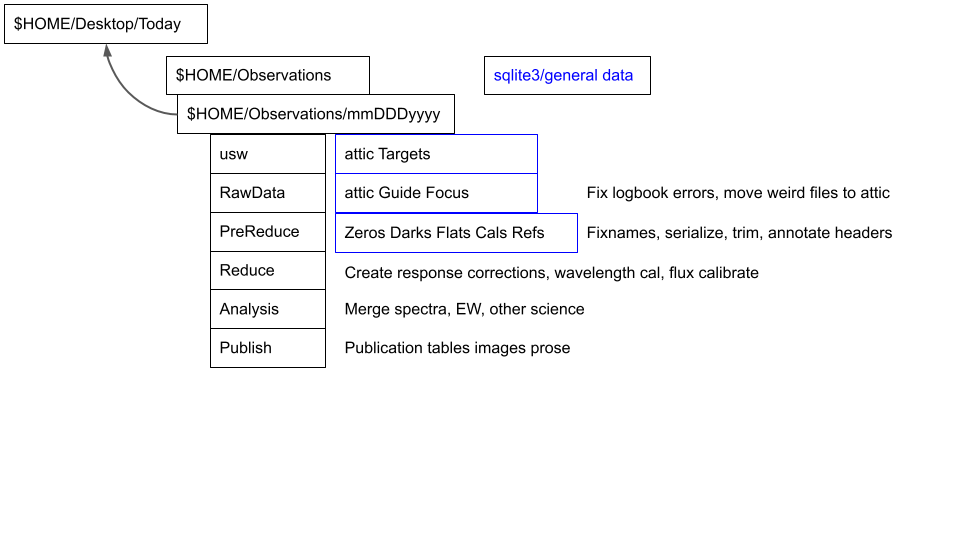
\includegraphics[width=.8\textwidth]{images/Overview1.png}
\caption{Basic Pipeline Steps} %% \caption{{\tiny{citation}}}
\label{figure:basicpipeline}
\end{figure}

\clearpage

\setcounter{section}{0}

\ifx\documentisdraft\drafttest
\linenumbers    %%%%%%%%%%%%% DRAFT
\fi

\clearpage
\pagenumbering{arabic}
%% \fancyfoot[ELF,OLF]{Go to: \hyperref[sec:contents]{Contents}}
%% \fancyfoot[ERF,ORF]{Go to: \hyperref[sec:index]{Index}}
%% \fancyfoot[ECF,OCF]{Page \thepage}

\fancyfoot[LF,OLF]{Go to: \hyperref[sec:contents]{Contents}}
\fancyfoot[RF,ORF]{Go to: \hyperref[sec:index]{Index}}
\fancyfoot[CF,OCF]{Page \thepage}


\section*{Overview}

This document refers to the new IRAF/Pyraf Noirlab 2.18 supported
Pyraf3 : \url{https://iraf.noirlab.edu/} and
\url{https://github.com/iraf-community/pyraf}.

The document covers details system setup for observing and reduction.
We are using a Raspberry Pi/libindi/Ekos for managing cameras and
other details. Once data is captured it is quickly copied to a more
stable platform for backup and reduction. We have IRAF/PyRAF installed
on the RPi to facilitate focus and quick tests of the images.

IRAF/PyRAF is considered a terminal based ``command line
environment'', a very flexible way to use small programs to achieve
large goals. GUI environments restrict users to 'canned' logic. Many
people are uncomfortable with command line work. It requires learning,
practice, and frequent use to maintain a fine edge needed for scientific
data reduction.

This \dhl{Bon Mots} document represents many tricks that one may use
to avoid editing temporary files by hand and to provide an audit trail
for projects.

Go to Section \ref{sec:complexexample} and briefly ponder the code with an
eye towards: ``What is this person thinking!''.

\section{Typography} \label{sec:Typography}

The typographic conventions used in these notes.

Here \llbox{k} means hit the ``k'' on the keyboard. 

\subsection*{Text}

The document uses \dhl{color} to make something \dhl{interesting},
stand out from the text.

\subsection*{Examples}

Examples, in general, state a \dhl{Goal}, the statement of the
\dhl{example}, and \dhl{Prose} to describe the 'thought model' or a
statement about takeaways from the example, and where needed some
exercises. These are presented in this format:

\begin{quote}
\goal Demonstrate a goal. Yes this example was a goal.\\ \example Give
an example of some syntax.\\ \prose Hey, put a linguistic pattern into
your ``thought process'' for that syntax.\\ \exercise[-a] Pick up your
pencil and start your notebook! \\ \exercise[-b] Time to stand for a
minute. \\ \takeaway Tie the thought process to a concrete goal and
example and begin documenting and checking your work.
\end{quote}

\subsection{Margin Annotations}

There are places in the notes where margin annotations are used
to draw attention to something important. In some cases this will
be a note to the author to add/clarify a section of text. Usually
more information may be found in the End Notes section of the document.
\ltodo{Example of Margin Note}{Added a note to demonstrate the note process.}

\subsection{Index}

This document is written in \LaTeX. The \LaTeX environment permits developing
and maintaining a set of bibliographic references, a great index and glossary. 

\section{The Unix and the Data ``Big Picture''}

This document is centered around the Ubuntu 22.04 LTS release using
the NOIRlab IRAF/PyRAF 2.18 pagkage. It offers a paradigm developed
over years of working with IRAF. This leverages Unix. The astronomy
community uses Apple Mac computers that still retain enough about Unix
to allow easy porting of IRAF and friends to that platform, even the
Apple Mx processors.

Win1X requires a VirtualBox (the Microsoft HyperV does not work well
enough).  The client operating system installed in the Virtual box may
be Fedora (the community version of Red Hat Enterprise Linux or RHEL).
This allows installing ESO packages that leverage the RHEL environment.
\textbf{Note}: Some AMD processors will not run hypervisors.
\index(RHEL!ESO) \index{RHEL!Win1X} \index(VirtualBox)

In Unix everything is a 'file'. Programs should be small, perform a
duty and do it well, permit some options. A program takes input from
``standard-in'' (\dhl{stdin}), does its work and puts its output to
``standard-out'' (\dhl{stdout}). Any errrors are reported via
``standard-err'' (\dhl{stderr}). Unix uses a device called a \dhl{pipe}
to send the output from one program into the stdin input of another.
Thus programs can be linked together on one line. 

OK, some programs are huge, and this paradigm does not necessarily
apply. But all the basic Unix utility programs like \dhl{ls}, \dhl{find},
\dhl{grep} etc work this way.

Changing from a GUI paradigm to a command line paradigm is one of the
hardest things for many reading these notes to do.

The Unix philosophy set forth by Ken Thompson, as documented by Doug
McIlroy \cite{McIlroy1978,McIlloryPhilosophy}:

\begin{quote}
Make each program do one thing well. To do a new job, build afresh
rather than complicate old programs by adding new "features". Expect
the output of every program to become the input to another, as yet
unknown, program. -- McIlroy
\end{quote}

GIUs are monolithic in design.\footnote{A GUI is a great way to encapsulate
a process where variation in the process is shuned and discouraged. Scientific
data is noisy and physics is opinionated -- this requires a careful attention
to detail not managable with GUI environments.}

One negotiates with Linux's root process to connect to the Linux
system, where the login process drops the user into a \dhl{shell}. There are
several shells to choose from -- here we will stick with \dhl{bash}
\index{bash}. \textbf{\emph{Note:}} \dhl{/usr/sh} defaults to an abbreviated shell
called \dhl{dash} on most Debian systems. \index{Unix Shell!intro}

\begin{quote}
``On a UNIX system, everything is a file; if something is not a file, it is a process.'' --
Machtelt Garrels, ``Introduction To Linux: A Hands On Guide''
\end{quote}

Peter Freeman \cite{freeman1975software} offered a model of a computer
(and a good operating system) as one of a \dhl{Processor},
\dhl{Memory} and \dhl{Transducer} (PMT) \index{computer!PMT}. The
processors today have less than one core to multiple cores, symmetric
arrays of cores and massively parallel cores.  Even the core of yore
is being supplanted by compute engines, the current popular one is the
GPU with $10^{\$}$ tiny cores.

Files are specialized and fall into classifications like: directories,
special files, links, sockets, named pipes.

There is only one file system and it starts at ``/'' or \dhl{root}.
We tend to think of files as residing on a disk drive. Multiple
drives, and their multiple partitions are simply ``mounted'' at
a location under the ``/''   root directory. Examples are
usually called something like /usr2. Disks on other machines
are usually found, conceptually as a sub-directory the /mnt directory.

\subsection*{The Shell ,``commands'', and Scripts}

The computer sees typed text as groups of characters separated by some
delimiter. Usually the delimiter is a combination of one or more
spaces and/or tab characters. These are called \dhl{whitespace}.

So all of programming takes a stream of complex symbols that, when
taken together, direct the computer to take some safe action. Linux
uses whitespace to set apart each symbol. 

Commands are designed to be typed at the keyboard and are usually
highly abbreviated. One of the handiest commands is \dhl{man}.

\example Use the ``\dhl{man}'' command \\
\prose Hey, what does the man (or ls or ln) command do?\\
\exercise Enter ``\dhl{man man}'' at the shell prompt.\\
\takeaway Read about how man works!\\
\exercise[-b] Enter ``\dhl{man ls}'' at the shell promot.\\
\takeaway Note: it says ``list directory contents'' so the abbreviation
of ``ls'' makes sense. It also offers up a myriad of options.\\
\exercise[-c] Try ``\dhl{ls -l}'' to see details of each file, one per line.\\
\takeaway A way to determine if files are normal files, directories or
links.

One of the oldest Unix commands is ``ls'' used to 'LiSt' directories and
their contents in interesting ways.

\section{Files and Directory Structure}

IRAF/PyRAF 2.18 is installed at a system level, and customized for each user.
The \dhl{mkiraf} command will create a {\textasciitilde}/.iraf directory.

IRAF uses two key files: \dhl{login.cl} and \dhl{loginuser.cl} to select from a myrid
of options and packages one will use for the tasks at hand. The \dhl{login.cl}
file now resides at \dhl{/etc/iraf/login.cl}. The loginuser.cl is located
at {\textasciitilde}/.iraf.loginuser.cl -- this is the file you change.
\textbf{\emph{Note}}: a single line with the word ``keep'' is required at the bottom
of this file.

The loginuser.cl file may be used to add your own special on-off commands,
and to leverage \dhl{foreign} tasks (usually other handy programs on the
path). \index{IRAF!foreign tasks}

Each IRAF task has a set of parameters, managed in the {\textasciitilde}/.iraf/uparam
directory. 

\textbf{BEWARE}: IRAF tasks are ``sticky''. When you change something it remembers the new
thing. The IRAF command \dhl{unlearn <task>} will cause the task to revert to
its defaults. \index{IRAF!sticky}

Other files:

\vspace{-.15cm}
\begin{enumerate}\addtolength{\itemsep}{-0.5\baselineskip}
%\setcounter{enumi}{N}
   \item  {\textasciitilde}/.bashrc, include your own {\textasciitilde}/.iraf-aliases
   \item  login.cl  - traditional configuration, don't edit this one.
   \item  loginuser.cl - configuration to users special taste.
   \item  pyraflogin.py - while not official has handy python functions
   \item  home\$/uparm - where the system keeps parameter files.
\end{enumerate}

\subsection{Directory Layout}

There are two quintessential things about data: 1) preserve the data
and 2) be able to audit processing of the data.

The most important thing is the preservation of the data. Backup,
Backup and Backup again. Then make a copy. It is best to save data on
multiple machines, or to the cloud. Google Drive (and other places)
offer 5TB of data storage for a quite reasonable fee.

All camera data consists of \dhl{16-bit unsigned ADU} values per pixel from
the camera. It is not necessary to change and/or archive raw data with
float values. The QHY600M images are 9600 x 6433 x 2 bytes of image,
roughly 13e6 bytes. Therefore 5TB of disk space will hold roughly
380,000 images. At 3 images per minute for an 8 hour night you get
2400 days of observations for 5TB of disk storage. That's 12 years in
practical terms. However, transferring these images over the net is a
problem.

% (iv (setq tmp (* 9600 6433 2)))    123513600  
% (iv (setq tmp (/ 5e12 13e6 )))    384615
% (iv (setq tmp (/ 384615 (/ 1440 3 3) 200 )))   12     2403

The \dhl{{\textasciitilde}/Desktop} directory allows software acquisiton software to be
configured once. Each night should be copied and archived. 

\begin{quote}
\begin{figure}[h!]
\dirtree{%
.1 {/home/user}.
.2 Observations.
.3 usw  - target lists, cl, notes, other generic things.
.3 ddMMMyyyy  - Date of sunset at Observatory.
.4 usw  - target lists, cl, notes, other generic things.
.4 RawData  - data: warts, blisters and all made read only.
.4 PreReduce  - copy RawData, and work here.
.4 PreAnalysis - pick up analysis for files.
.4 Reduce - Major IRAF/NonIraf reduction.
.4 Analysis - Major IRAF/NonIraf analysis.
.2 Desktop.
.3 Today - where all ``tonights'' observations go.
}
\label{figure:dirlayout}
\end{figure}
\end{quote}


The directory \dhl{usw} is used in lieu of etc. It is the German language
way of saying the samething - \dhl{und so wieder} ``and so again''.
In Unix \dhl{etc} contains loosely related information. For example
puruse \dhl{/etc}, where the system keeps configuration information
of a global level. It is so overloaded something unique is desired.

With this layout, the \dhl{{\textasciitilde}/Observations/usw}
directory contains side files of importance your overall personal
observing strategy. Files, like ds9 region files, special catalog
files general tools etc are stored here. Make subdirectories that
hold common information for different sites or instruments. Copy
those data into a nightly structure as needed.

Data is taken at night. Use dates that reflect the date of sunset
at the site where the data were obtained.

Using the KStars/Ekos/libindi, running on a Raspberry Pi for example,
or a local machine you may want a \dhl{{\textasciitilde}/Desktop/Today} directory
for each night's observing run. In this way the capture/observatory
software does not have to be configured each night. That export directory
remains the same. At the end of the night, simply rename the directory.

Date formats may be confusing, and subject to a computer's LOCALE
subsystem Nobody can make their minds up about date formats.

\centerline{{\huge{{\color{darkred}{SO! SPELL THE DATE OUT!}}}}}

The \dhl{ddMMMyyyy} directory uses the 1 or 2 digit day of month,
followed by the text abbreviation of the month, followed by a 4-digit
year (lets don't play Y2K again). 

This format makes the shell's text completion a quick way to move around.
Text completion involves typing a few starter characters of the file/directory
name then hit the tab. It will advance to the next non-unique thing.

Underneath \dhl{ddMMMyyyy} is the usw directory for tonight's work. The
target list, special catalog file of reference stars etc, the scheduler's
input. Here we store the \dhl{reduce.cl} or \dhl{reduce.py} script
template to be developed for these particular data.

The RawData/PreReduce/PreAnalysis/Reduce/Analysis directories are
cascading stages of data. You may use an \dhl{attic} directory where
to sideline unrelated or terrible images.

You can automate file reduction by using sub-scripts/tasks within the
melange of IRAF/PyRAF/bash/python/whatever language programs and then
leveraging Python and cl into making a
\dhl{OBSERVATION/usw/reduce.pyraf}\index{reduce.cl}
script\index{reduce.pyraf} script for the data. Save this as a template in
the general \dhl{usw} directory, and copy in to each observation's repository.
Detailed example is in Appendix \ref{sec:ReducePyrafControlFile}.

At this time PyRAF (a mix of ecl and Python) does not act well as a
``script'' due to the hack that adds ecl syntax to the GNU runline command
input. It uses the raw input directly and side-steps \dhl{stdin}. This
violates the Unix philosophy of each program should take its input from
stdin, process its results and put the results into stdout.  This
allows one to pipe programs together to achieve an ultimate goal.

Scripts may be written in the \dhl{.cl} language (really ecl or extended cl),
actual PyRAF (\dhl{.pyraf}), or hacked into PyRAF with the \llbox{!}
cl prefix as you go along.

\textbf{\emph{Note}}: The \dhl{.pyraf} scripts blend python and PyRAF together.
See the complicated example of how to deal with APO NICFPS camera
images.

\section{Critical First Steps}

It is critical you properly install the IRAF/PyRAF3 packages. This
release looks for a {\textasciitilde}/.iraf directory that may not be fully integrated
into the rest of IRAF.

You may make a soft link of \dhl{\home/iraf} to \dhl{\home/.iraf}:

\dhl{ln -s \home/iraf \home/.iraf}

The document will continue to refer to \dhl{\home/iraf} as the base
of the IRAF package. 

It is important to use a \dhl{~/iraf/loginuser.cl} file with task
aliases foreign and tasks.\index{tasks!aliases} \index{tasks!foreign
  tasks}

One way to make things simple is to create a bash alias for pyraf that:
\vspace{-.15cm}
\begin{enumerate}\addtolength{\itemsep}{-0.5\baselineskip}
%\setcounter{enumi}{N}
   \item   uses xdotool to change the color of the window's background
   \item   update the PATH and PYTHONPATH to access all the special files you use
   \item   run the system pyraf (note the /usr/bin path is prefix is necessary) 
 with the ``-s'' switch for ``silent'' start.
\end{enumerate}


\begingroup \fontsize{10pt}{10pt}
\selectfont
%%\begin{Verbatim} [commandchars=\\\{\}]
\begin{verbatim} 
alias pyraf="xdotool key shift+F10 r 1;\\
  export PATH="/usr/local/bin:$PATH"; export PATH="/usr/local/astrometry/bin:$PATH";\\
  export PYTHONPATH=$HOME/.iraf; export PATH="$HOME/.iraf/smtsci/bin:$PATH";\\
  /usr/bin/pyraf -s;"
\end{verbatim}
\endgroup
%% \end{Verbatim}

\subsection{IRAF/PyRAF Tasks and Packages}

IRAF, from ye-olden times, uses \dhl{packages} containing help text
and parameter files to hold values from run-to-run together with the tasks'
executable code.
\index{IRAF!tasks} Tasks are ``programs'', usually written in FORTRAN
or in cl proceedural code. Some are written in C/C++.

\dhl{BEWARE}: IRAF is \dhl{sticky}! It retains parameter values from
run-to-run that can perpetuate errors. Review all the parameters to be
sure your reductions are proper. These values are stored in the
\dhl{~/iraf/uparm} directory.

Tasks are built into IRAF/PyRAF but are only loaded once. Each time
they are used -- they are in memory and already part of the CPU thread
you are using. Thus they very fast. Using \llbox{!} shell-escape or a
\dhl{\$foreign} task causes Unix to create a new heavy-thread with
significant overhead (especially in a loop).

IRAF has a habit of loading images into memory and keeping them there.
Some tasks will modify the in-memory image but not write it back to
the disk. Work may be lost. See Section \ref{sec:FITSFiles} for quick
details.

IRAF has a neurotic habit of \dhl{sometimes} adding an extent to
certain FITS files! This is the case with master darks and flats
and a handful of other operations.

It is best to develop your \dhl{reduce.pyraf} script in an editor, one line
and step at a time, then cut/paste edited lines at the interactive
prompt. When you make a mistake -- and you will -- you can start over
with a fresh copy of data and stop short of the mistake. Pick up and
go again.

\subsection{Full On Python Hacks}

\example Python's \dhl{import iraf} statement allows for operations like: \\
\prose I want to use IRAF's imstat command to get a binary value, assign
the value to my python variable. \\
\exercise Enter: \\
{\color{verbcolor}{
\begingroup \fontsize{10pt}{10pt}
\selectfont
%%\begin{Verbatim} [commandchars=\\\{\}]
\begin{verbatim} 
mymean = float( iraf.imstat(images='*fits',fields='mean',format=iraf.no,Stdout=1)[0])
\end{verbatim}
\endgroup
%% \end{Verbatim}
}}

\takeaway The task has a pythonic wrapper, contained in the iraf.py
module's namespace.  It needs a list of files, we only want the one
field \dhl{mean}, we do not want the headers (format=iraf.no). The
phrase Stdout=1 (note capitalization) returns the text as a string
rather than printing on the terminal. But! The string is actually an
array, so we want the first bit. But! that bit is a string, and we
need to convert to binary with the \dhl{float} python function.

where \dhl{mymean} is now a proper python float. Yes, convoluted, but
its buried in a scrip and available for your use. \index{Stdout}

\subsection{Task Parameters}

Always be aware of the:
\vspace{-.15cm}
\begin{enumerate}\addtolength{\itemsep}{-0.5\baselineskip}
%\setcounter{enumi}{N}
   \item    ~/iraf/uparm directory
   \item    lparm <taskname> command to list parameters.
   \item    \dhl{unlearn <task>} command.
   \item   help <task> and look at the see also part at the bottom.
\end{enumerate}

\section{Goals}

The main goal of scripting is not the script, it is the result. Good
data results do not come from good scripting -- but come from good
planning, good execution of the plan and attention to configuring
your tools.


\subsection{Things to remember}

IRAF \dhl{cl} morphed into PyRAF \cite{2006hstc.conf..437G} to allow a more
powerful \dhl{cl} by hacking the Python \dhl{readline} subsystem. The
grammar of python was altered to allow for a ``direct entry'' of most older
\dhl{cl} commands. Direct access to the underlying tasks was
accomplished with a ``cythonic'' interface into underlying code. An ``iraf''
module was added to support programming calls to IRAF tasks and using 
a special Python \dhl{keyword} argument Stdout to return output as a string.
Parsing this string with python allows chaining \dhl{cl} commands together
for a goal.

A tremendous amount of power is available for you to mix and match to meet
your specific needs. 

\subsection{Observation Directory}

One can not expect proper structure by simply importing a night's
observations, warts blisters and all. Files will be scattered all
over, mis-named, bad headers, useless(!), and other oddities. But copy
the data into date/RawData. See directory layout table \ref{figure:dirlayout}

Open date/usw/reduce.cl in your favorite editor. Anything you want
to type into PyRAF -- type it into the reduce.cl file. Then cut/paste
the command to PyRAF. This means when you make the mistake -- you
can remove the last line, save the reduce.cl file, and rebuild
to that point. Yes, some interactive things will or may happen.
Try not to make too many mistakes.

\vspace{-.15cm}
\begin{enumerate}\addtolength{\itemsep}{-0.5\baselineskip}
   \item   cd ~/Observations
   \item   mkdir 22Feb2022 \# date of sunset at the observatory
   \item   cd 22Feb2022
   \item   mkdir -p Plan RawData PreAnalysis Analysis Publish usw
   \item   mkdir -p PreAnalysis/{Bias,Darks/{s300,s3},Flats,Comps} \# prior knowledge
   \item   cd RawData
   \item   cp -pr /mnt/NAS/22Feb2022/* .  \# copy the raw data
\end{enumerate}

Now the plan for observations and initial PreAnalysis results is in 
place. The \dhl{usw/reduce.cl} script is the key. 

Good observations are the result of good planning. Make the list of targets,
determine offsets and guide stars, create a ds9 region file in ICRF WCS
coordinates for the field of view and possible orientations of the instrument.
If possible download the preparation package from the observatory and take
time to prepare. \index{planning}

\begin{figure}[h!]
\centering
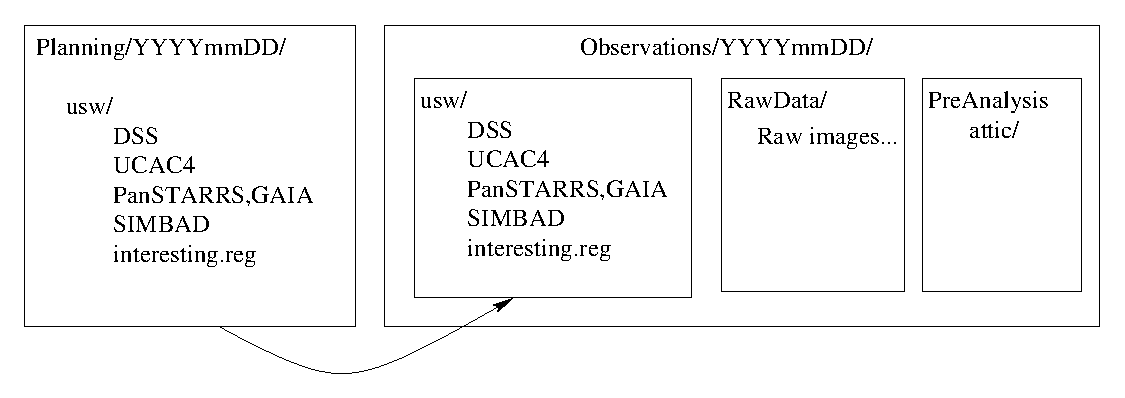
\includegraphics[width=.4\textwidth]{images/Overview.eps}
\caption{The observations directory was in place with the plan.
Load up the raw images. Then copy raw data to pre-analysis.} %% \caption{{\tiny{citation}}}
\label{figure:GoalsOverview}
\end{figure}

\clearpage
\subsection{The main tricks}

Note: Unix files do not rely on their extensions. A Unix extension is a social
convention. Many authors use two files, like \dhl{in.txt} and \dhl{out.txt}.
They will use an editor to change the bits of one to another. 

I recommend using goofy file names, like \dhl{xxx} and \dhl{l.l}, when seen
they may be removed. The filename \dhl{l.l} is real easy to type because
the \llbox{l} and \llbox{.} are right next to each other!

The \llbox{/}\llbox{/} sequence is the cl concatenation operator, used to
join two strings without intervening whitespace.

Instead of having the input files in in.txt, then editing to make unique
output names -- simply prepend a string, with some meaningful context
to the @file. 

The order of operations may be to
\vspace{-.15cm}
\begin{enumerate}\addtolength{\itemsep}{-0.5\baselineskip}
%\setcounter{enumi}{N}
   \item   t\_ trim a file.
   \item   c\_ cosmic ray removal
   \item   z\_ to zero correct
   \item   d\_ to dark correct
   \item   f\_ to flat a file
\end{enumerate}


etc. data.fits, after processing may be \dhl{f\_d\_z\_c\_t\_data.fits}.

So PyRAF has several tricks up its sleave:
\begin{itemize}
\addtolength{\itemsep}{-0.5\baselineskip}
   \item   It can act like a basic ``calculator'' just by typing standard python at the
PyRAF command prompt. Remember to ``import'' packages like math and numpy.
   \item It works with list of files. These are refered to as ``list''
     or ``at'' files. They are like {\color{verbcolor}{\verb#@l.l#}}
     where the file ``l.l'' has a list of filenames -- one per line.
   \item You can take the files in ``l.l'' and produce new files with
     the same name but prepend a clause to the
     filename!\\ \textbf{E.g.:}
     {\color{verbcolor}{\verb#imarith @l.l - zmaster.fits z_//@l.l#}}\\ will
     subtract the zero master from each file in ``l.l'' and make a
     corresponding {\color{verbcolor}{\verb#z_filename.fits#}}.
\item PyRAF is a a replacement for {\color{verbcolor}{\verb#cl#}} (actually
ecl). You can loop {\color{verbcolor}{\verb#.cl#}} commands together
with bash commands into the mix to do work using:\\
{\color{verbcolor}{\verb#cl < ~/iraf/fit2fits.cl#}} to bring a Vendor's
fit format to the PyRAF standards.
\end{itemize}

It has a few oddities, inherited from the ecl lashup of the Pythonic 'readline' hack,
ripped from a \dhl{reduce.cl} script:

\vspace{-.15cm}
\begin{enumerate}\addtolength{\itemsep}{-0.5\baselineskip}
   \item Oops! Its Python 2.7 so write helpers like \dhl{trim} and
     \dhl{fitsls} accordingly.
   \item   Most of the IRAF \dhl{cl} commands work
   \item   \dhl{set OBSROOT=/home/me/Observations/23Feb2022}
   \item   \dhl{set OBS=OBSROOT\$/PreAnalysis}
\end{enumerate}

The IRAF command \dhl{chdir} \index{cl!chdir} changes directory while respecting
the IRAF use of iraf-environment variables.

You can escape to bash by starting the line with a bang (!). This
allows developing handy bash scripts to store in iraf/bin.

\clearpage

\subsection{System Setup}

I presume the use of the Ubuntu 22.04 Linux distribution from Canonical\texttrademark.

%% Under Microsoft Windows\texttrademark Pro, there is a system called \dhl{Hyper-V}.
%% It is very ``light-weight'' virtualization layer for Windows that permits
%% the seamless of an essentially containerized Ubuntu 22.04 + anaconda and other
%% Linux based tools while maintaining contact with the Windows file system,
%% the network etc. \index{Windows!Hyper-V}.

%%Under Linux you are running Linux anyway.
MacOS is very Linux like, even on their M1 processor series.

Install the Anaconda package without the Navigator. This brings in
a massive amount of power, including Astropy \cite{astropy:2013} \cite{astropy:2018}
\cite{astropy:2022}.
\vspace{-.15cm}
\begin{enumerate}\addtolength{\itemsep}{-0.5\baselineskip}
   \item    Necessary:
\vspace{-.15cm}
\begin{enumerate}\addtolength{\itemsep}{-0.5\baselineskip}
   \item    Ubuntu 22.04/Mac OS + many apt-get packages
   \item    Anaconda (Python 3+)
   \item    Astroconda PyRAF recipe (a python2.7 env)
   \item    Ubuntu aptitude iraf/pyraf packages
   \item    Sextractor
   \item    Current SAOImage/ds9
   \item    Current Astrometry.net + 4200 and GIAI data
   \item    Fitsverify \cite{fitsverify-1}
   \item    GitHUB sasiraf package (currently private contact author.)
\end{enumerate}
   \item    Optional
\end{enumerate}

\subsection{Unix\texttrademark Aliases}
A few aliases need to be setup.

\ltodo{Add Aliases}{Update/add aliases for bashrc file.}

\begin{figure}
{\color{darkred}
\begingroup \fontsize{10pt}{10pt}
\selectfont
%%\begin{Verbatim} [commandchars=\\\{\}]
\begin{verbatim} 
function pyraf  { #export PYTHONPATH=$HOME/iraf;
                  export PATH="/home/wayne/anaconda3.8/envs/geminiconda \\
                     /bin:$HOME/iraf/smtsci/bin:$PATH"; (folded line)
                  source activate geminiconda;
                  xdotool key shift+F10 r 6;     # change terminal color
                  $HOME/anaconda3/envs/geminiconda/bin/pyraf -s $*;
                }
\end{verbatim}
\endgroup
%% \end{Verbatim}
}
\caption{An entry into the aliases file, using the Gemini pyraf installation.}
\label{fig:geminialias}
\end{figure}

This is a little-bit complicated:
\vspace{-.15cm}
\begin{enumerate}\addtolength{\itemsep}{-0.5\baselineskip}
   \item   The PYTHONPATH allows pyraflogin3 to be imported after start.
   \item   This assumes \dhl{~/iraf/pyraflogin.py} is present.
   \item   The function in figure \ref{fig:geminialias} tells Anaconda to activate
     the geminiconda environment
   \item   The xdotool allows the color of the terminal window to be changed.
   \item   PyRAF is then started, the \dhl{-s} switch is quiet about packages loaded.
   \item When pyraf starts, it loads \dhl{login.cl} which in turn
     loads my \dhl{loginuser.cl} scripts.
\end{enumerate}

\subsection{Initialization files}

PyRAF uses \dhl{~/.iraf/login.cl} to manage system level commands and should
not be edited -- except to ensure that \dhl{cl < "home\$/iraf/loginuser.cl"} is
enabled. Edit the \dhl{loginuser.cl} file and pile changes.
 \index{Initialization!login.cl}
\index{Initialization!loginuser.cl}

A special \dhl{~/iraf/pyraflogin.py} file can 'extend' the Python
environment.  A sample file is available with this package. It
requires the special alias to start PyRAF. It adds simple
\dhl{matplotlib} plotting and some handy fixer-upper functions. See
that package for documentation. \index{Initialization!pyraflogin.py}

\subsection{Initial Steps}

This process uses a user-defined  directory structure as shown in
figure \ref{figure:basicpipeline}. 

The main steps are:
\vspace{-.15cm}
\begin{enumerate}\addtolength{\itemsep}{-0.5\baselineskip}
   \item   Layout basic directory structure:


   \item  Add a few toplevel soft-links for non-sentient file browsers.
\dirtree{%
.1 \$HOME/.aaatoday linked to \$HOME/Desktop/Today.
.1 \$HOME/.aaareduce linked to current working reduction.
}

   \item   Planning - load up the \dhl{\$HOME/Desktop/Today/usw} directory with
FOV files, and anything related to observatory etc.

   \item   Observe
   \item   Move dhl{\$HOME/Desktop/Today} to dhl{\$HOME/Desktop/Observations/mmDDDyyy}
date of sunset at the observatory of the instrument.
   \item   Make a safe backup.
   \item   Start the process of reducing the data.
\end{enumerate}

The script provides the audit trail you used. Modify this for each
instrument setup, and for each filter type etc.  Essentially the same
for spectroscopy -- just watch the statistics sections.

You may not need darks, and the flats will be different.

When, not if, you mess up you can delete the PreAnalysis directory, fix
the above script, and start over. As you move deeper into the file
processing, the script becomes more valuable.


\clearpage
\subsection{PyRAF Calculator Mode}

\goal Demonstrate borrow Pyraf as a calculator within PyRAF. Determine
the mean plus 3 times the standard deviation for a limit.

\example 
{\color{verbcolor}{\verb#imstat zmaster.fits fields=mean,stddev#}} \\
you find the mean is 346 and the stddev is 47.

\exercise How many pixels in the zero master are 3 or 5 $\sigma$ above
the mean?

{\color{verbcolor}
\begingroup \fontsize{10pt}{10pt}
\selectfont
%%\begin{Verbatim} [commandchars=\\\{\}]
\begin{verbatim}
from astropy import fits  # DO THE IMPORTS ONCE
import numpy

f = fits.open('zmaster.fits')    # open the fits file as a cfitsio like
d = f[0].data   # get the data   # structure and just grab the data.
# using some python magic!
(mean,stddev) = map(float,
                   iraf.imstatistics(Stdout=1,fields='mean,stddev',
                      images='zmaster.fits',format=iraf.no)[0].split())
len(d[d> mean + 3.0*(stddev)]) # 25729 pixels matched this example
len(d[d> mean + 5.0*(stddev)]) #  1220 pixels matched this example
f.close()
\end{verbatim}
\endgroup
%% \end{Verbatim}
}


\prose Hey, we're PyRAF, a pythonic interpreter -- so lets really use
Python.  The imports are used to get the modules/functions we
need. The fits.open gets the FITS file open for business; we grab just
the image data as a numpy array of shape
{\color{verbcolor}{\verb#NAXIS2,NAXIS1#}} (switched(!), numbered from
zero now and the data will have overscans if present!) using
{\color{verbcolor}{\verb#d = f[0].data#}}. The
{\color{verbcolor}{\verb#iraf#}} is imported by virtue of we're PyRAF;
the {\color{verbcolor}{\verb#imstat#}} is run as a python function
using {\color{verbcolor}{\verb#iraf.statistics()#}}.  The
{\color{verbcolor}{\verb#Stdout=1#}} tells the task to return the
output not send it to the terminal. The
{\color{verbcolor}{\verb#format=no#}} tells the function to omit the
usual header text etc, and just return the two values requested with
the {\color{verbcolor}{\verb#fields="mean,stddev"#}}.  The output is
one string with two ASCII numbers. These are split into an array, then
the {\color{verbcolor}{\verb#float#}} function converts the strings
into actual numbers -- returned as the tuple
{\color{verbcolor}{\verb#(mean,stddev)#}}.

\subsection{Using Numpy Arrays}
%HEREHEREHERE

Numpy arrays follow the ``C'' indexing scheme, which is ``ordinal'' in nature
(starting with zero). For an (X,Y,Z) index -- the array is referenced \dhl{backwards}:
myarray[Z][Y][X]. This differs from the FORTRAN convention for arrays, ``cardinal''
in nature (counting from 1).

FITS images are stored in FORTRAN order, and in Big Endian format. This makes
difficult for Intel architectures.

This is critical. Data are written into FITS images in so-called \dhl{Big-Endian}
fashion. In Jonathan's ``Gulliver's Travels'', a fictional character encounters
a culture in heated conflict over weather or not one should crack open an
egg on the little end or the big end. Computer aritectures are conflicted on
how to store a larger value, say an integer that spans more than one byte
into a linear address space. Decisions (bad perhaps) were made to store
a 16-bit integer with the byte containing least significant digit first.
The word oxBO is stored with the 0 first then the 0x0B. This was to make
a very early machine fast at ++value operations! We're stuck with that decision
since.

The real issue boils down to the Bad Thing\texttrademark practice of
``type punning'' whereby a block of data in ``Endianess Be Damed''
format is read into memory, then attempts to access it as though it
had the right byte order results in catastropy when data is exchanged
between the types of architectures.

Intel processors are ``Little Endian'' where processors like the Motorla
68000 were ``Big Endian''. 

Data are stored as arrays, with astropy.fits.io open command setting the
data[0] extent as a pythonic numpy array. So the indices are a bit backwards
The fits header would read something like:

\begingroup \fontsize{10pt}{10pt}
\selectfont
%%\begin{Verbatim} [commandchars=\\\{\}]
\begin{verbatim} 
NAXIS  = 2
NAXIS1 = 2048
NAXIS2 = 512
\end{verbatim}
\endgroup
%% \end{Verbatim}

To store a 2D image array. This is ment to denote an image that is 2048 wide and 512
tall. 

\ltodo{numpy vs FORTRAN}{Get into index details.}


The next bits use numpy arrays. Here we use the conditonal indexing
mode common to numpy arrays to get all the pixels that match
expression of the value > the
{\color{verbcolor}{\verb#mean + n times stddev#}}.

Need a ``Quick Calculation'' to find the center of an image to
use as a ``statistics section'' for normalizing?:

{\color{verbcolor}
\begingroup \fontsize{10pt}{10pt}
\selectfont
%%\begin{Verbatim} [commandchars=\\\{\}]
\begin{verbatim}
imhead zmaster.fits   # result is 'zmaster.fits[1368,1364][real]:'
# half size? pick up the [NAXIS1,NAXIS2] from abbreviated imhead result...
(1368//2, 1364//2)   # returns tuple (684, 682)  the '//' is integer divide.
print "[%d:%d,%d:%d]" % (1368//2 - 50, 1368//2 + 50, 1364//2 - 50, 1364//2 + 50)
# [634:734,632:732]  Et Viola! A handy center stat section for normalizing!
\end{verbatim}
\endgroup
%% \end{Verbatim}
}

Make your own functions! Then imexamine -- the comp star and the target star.

{\color{verbcolor}
\begingroup \fontsize{10pt}{10pt}
\selectfont
%%\begin{Verbatim} [commandchars=\\\{\}]
\begin{verbatim}
import math    # DO THIS ONCE
def mag(compmag,compflux,observedflux):
   return -2.5(math.log10(observedflux / compflux) + compmag
\end{verbatim}
\endgroup
%% \end{Verbatim}
}

\exercise Correct for background.

\section{Getting Started}

Configure the system. Copy the login.cl to ~/.iraf. Copy loginuser.cl script
to ~/iraf. \textbf{\emph{Note}} One has a hidden-file dot.

Add the .iraf.aliases file to \dhl{\$HOME} directory and if you like, add it to
the \dhl{\$HOME/.bashrc} file.

Start PyRAF in one window and start Editor in another window. I
recommend emacs or Sublime Text as editors -- they are GUI
oriented. Remember all things have a learning curve.

Why we use the vi editor. Vi is the ``\dhl{Vi}sual Editor'' that sits
on top of a powerful albeit basic Unix editor ``\dhl{ed}. The \dhl{ed}
editor is the basis for the \dhl{sed} the Unix stream editor. Regular
expressions (think wildcards) are very sophisticated and turn up all
over the Linux/Unix system. They are worth the effort to learn. The
``re'' of the grep program (\dhl{g}lobal \dhl{re}gular expression
\dhl{p}rint) program obviously makes heavy use of regular expressions.

The very basic Linux commands are:

\begin{table}[h!]
\centering
\begin{tabular}{| l | l |}
\hline
Command  & Basic Action   \\
\hline
cd    & change directory    \\ 
ls    & list files     \\ 
pwd   & print the current working directory    \\ 
cat   & \dhl{concatenate} file(s)    \\ 
less  & view content of a file    \\ 
man   & the Manual -- print details of a command \\ 
which & show where on PATH an executable is \\ 
rm    & remove files and directories. \\
%% ones-based: \cline{a-b}
\hline
%%\DeleteShortVerb{|}
\end{tabular}
%%\end{minipage}    %% for footnotes  r@{.}l 
\caption{Very Basic Unix Commands}
\label{table:VeryBasicUnixCommands}
%%} % end small etc
\end{table}


\subsection{Very Basic PyRAF commands}

\begin{table}[h!]
\centering
\begin{tabular}{| l | l |}
\hline
Command  & Use   \\
\hline
cl            & run the cl editor                            \\
epar          & edit parameters/launch task                  \\
hedit         & fast/dirty header editor                     \\ 
imhead        & list the header values for a file            \\ 
hselect       & select values from headers                   \\ 
imexamine     & all manor of ways to view images             \\ 
apall         & reduce a spectrum image                      \\ 
identify      & identify spectral lines assign wavelenghts   \\
dispcor       & apply identify results to science spectrum   \\
splot         & view/analyze reduced spectrum                \\ 
imstat        & print mean,min,max,std etc for set of images \\ 
%% ones-based: \cline{a-b}
\hline
%%\DeleteShortVerb{|}
\end{tabular}
%%\end{minipage}    %% for footnotes  r@{.}l 
\caption{Very Basic IRAF/PyRAF commands}
\label{table:VeryBasicIRAF/PyRAFcommands}
%%} % end small etc
\end{table}


\section{Working on subsets of files.}

IRAF uses ``list files'' denoted \dhl{@list.txt}. The \llbox{@} key
as the first character of the filename tells IRAF to open that
file and take from it filenames -- one filename per line. This is
real handy.

Some documents have you make lists, then use an editor to change the
list as you go. They recommend filenames like mylist.txt. This is
cumbersome to type. Try using a simple name like \dhl{l.l}. Note the
\llbox{l} key is very near the \llbox{.} key! Handy to type.  If you
see the file \dhl{l.l} you know you can simply remove it.  The \llbox{!}
as the first character on a command line sends the rest of the line
to the local bash script. This escape mechanism allows you to use
all the power of Unix inside cl scripts.

The command \dhl{!ls -1 *Dar* > l.l} takes all filenames with Dar
in it and lists them out in lexicographical (sorted) order. Here
are some example of ways to build list-files.

{\color{verbcolor}
\begingroup \fontsize{10pt}{10pt}
\selectfont
%%\begin{Verbatim} [commandchars=\\\{\}]
\begin{verbatim}
!ls -1 *fits > l.l
cl < ~/iraf/crall.cl
# all the files are now c_<filename>

hselect c_*fits $I "IMAGETYP ?= 'Bias'"  > l.l
hedit @l.l IMAGETYP zero add+ show- ver- update+
!if test -e zmaster.fits; then rm zmaster.fits; fi  # bash to rm file if exists
imcombine @l.l zmaster.fits combine=median

hselect c_*fits $I IMAGETYP ?= 'Light'"  > l.l
hedit @l.l IMAGETYP object add+ show- ver- update+
imarith @l.l - zmaster.fits z_//@l.l
imarith z_//@l.l - dmaster.fits d_z_//@l.l
imarith d_z_//@l.l / flatmaster_SII.fits f_d_z_//@l.l

# files are now {\color{verbcolor}{\verb#f_d_z_c_filename.fits#}}
\end{verbatim}
\endgroup
%% \end{Verbatim}
}
This makes use of the fact that we can pile on prefixes to
processed files:

\begin{itemize}
\addtolength{\itemsep}{-0.5\baselineskip}
   \item   t - trimmed
   \item   c - cosmic ray reduced
   \item   z - zero subtracted
   \item   d - dark corrected
   \item   f - flat normalized
\end{itemize}

At the end, a flat-normalized file called {\color{verbcolor}{\verb#science.fits#}} will
have the name {\color{verbcolor}{\verb#f_d_z_c_t_science.fits#}}.

Lots of intermediate files lying around: Clean them up!

{\color{verbcolor}
\begingroup \fontsize{10pt}{10pt}
\selectfont
%%\begin{Verbatim} [commandchars=\\\{\}]
\begin{verbatim}
print "Remove residual files."
! (export LC_ALL=C; rm [a-z]_*fits 2> /dev/null;)
\end{verbatim}
\endgroup
%% \end{Verbatim}
}

\textbf{\emph{Prose:}} \textbf{\emph{Hey}} PyRAF send the line to bash; but! using a sub-shell
set {\color{verbcolor}{\verb#export#}} the {\color{verbcolor}{\verb#LC_ALL=C;#}}
shell variable to let bash actually use case sensitive wildcards. Then
{\color{verbcolor}{\verb#rm [a-z]_*fits 2> /dev/null;#}} remove the
file -- and in case there is some whining about the process, send the
whines to the bit-bucket ({\color{verbcolor}{\verb#/dev/null#}}).


\section{Observing}
PyRAF \index{PyRAF!Observing} is a useful tool for spectroscopy. Using
the imexamine command and the 'j' key: set the rplot to wider than a bright
line width. 

% HEREHEREHERE

\clearpage
\section{Overall Philosophical Approach}

This document covers a philosophy --- a set of general tools and
scripts to take and reduce data.

In this case some location like {\color{verbcolor}{\verb#/opt/myobs/iraf/#}}
or {\color{verbcolor}{\verb#~/iraf/#}} contains a number of small generic
{\color{verbcolor}{\verb#.cl#}} scripts to handle specific needs. These
are specific to certain conditions -- like a package that writes {\color{verbcolor}{\verb#.fts#}}
instead of {\color{verbcolor}{\verb#.fits#}} files. Routines to remove pesky
spaces that GUI users like to use; get rid of multiple ``dots''; plus signs
etc. 

\vspace{-.15cm}
\begin{enumerate}\addtolength{\itemsep}{-0.5\baselineskip}
   \item   Create a planning directory. Rename to Observations/directory
when the plan is executed.
   \item   Create a ``usw'' directory to hold the plan, collect pre-analysis information:
\vspace{-.15cm}
\begin{enumerate}\addtolength{\itemsep}{-0.5\baselineskip}
   \item   DSS image -- ds9 Analysis \menu Image Servers
   \item   Region files, catalog files for ds9 -- ds9 Region \menu Shape ...
   \item   Photometry reference stars --- ds9 Analysis \menu Catalogs \menu Database \menu UCAC4;
or with the Aladin application and TOPCAT make one the hard way. (PanSTARRS DR1).
   \item   Bibliographic information -- Browser and SIMBAD for the target(s).
   \item   Gather any existing bad pixel masks -- previous runs; observatory supplied files.
\end{enumerate}

   \item  Gather raw data --- stay up all night
   \item  Archive raw data as a RawData and make read only --- back to your {\color{verbcolor}{\verb#Observations#}} directory:\\
{\color{verbcolor}{\verb#(cd Observations/YYYYmmDD; mkdir -p RawData; cd RawData; rsync <from somewhere> .; chmod -w -R *#}}).
\end{enumerate}


\vspace{-.15cm}
\begin{enumerate}[resume]\addtolength{\itemsep}{-0.5\baselineskip}
   \item   Copy raw data to a PreAnalysis directory -- do not damage any
raw data whatsoever. Make the PreAnalysis files writable:\\
({\color{verbcolor}{\verb#cd Observations/YYYYmmDD; mkdir -p PreAnalysis; cd PreAnalysis; cp -pr ../RawData/* .; chmod +w -R .#}})\\
Clean data and make initial analysis files:
\vspace{-.15cm}
\begin{enumerate}\addtolength{\itemsep}{-0.5\baselineskip}
   \item   Fix the filenames --- {\color{verbcolor}{\verb#cl < ~sbo/iraf/fix_sbig.cl#}}
   \item   Fix the headers--- {\color{verbcolor}{\verb#cl < ~sbo/iraf/fix_headers.cl#}}
   \item   Trim (remember) overscan --- see above
   \item   Remove bad WCS especially from zero/dark/flats {\color{verbcolor}{\verb#cl < ~sbo/iraf/fix_sbig_wcs.cl#}}
   \item   Remove cosmic rays ---  {\color{verbcolor}{\verb#!ls -1 *fits > l.l#}}
followed by {\color{verbcolor}{\verb#cl < ~sbo/iraf/crall.cl#}}
\item Other basic reduction steps to be covered elsewhere:
\begin{enumerate}\addtolength{\itemsep}{-0.5\baselineskip}
   \item   Make any bad pixel masks 
   \item   Make master zeros and darks 
   \item   Make master flats 
   \item   apply zeros,darks,flats to science images
   \item   add new WCS or de-distort and add new WCS
   \item   extract photometry
   \item   combine images for deeper photometry
   \item   freeze this work
\end{enumerate}
\end{enumerate}


   \item  Copy the PreAnalysis data into an Analysis Directory.
(Any damage here is quickly recovered from PreAnalysis.)\\
{\color{verbcolor}{\verb#!(cd ..; mkdir -p Analysis; cd Analysis; cp -pr ../PreAnalysis/f_d_z_c_t* .)#}}
\end{enumerate}


A break down of the above steps reveals the need to make/use
certain scripts (some shown in red in context above):

\vspace{-.15cm}
\begin{enumerate}[resume]\addtolength{\itemsep}{-0.5\baselineskip}
   \item   Fix the filenames: remove dots, spaces, dashes other special characters.
   \item   Fix the headers: Observatory/Vendor non-IRAF keywords to IRAF
keywords; Very-Non-Standard keywords like PCOUNT and GCOUNT
   \item   Pinpoint is good enough for tracking (still takes a while to apply
and will fail) but is not accurate.
   \item   Single Pixel errors from cheap cameras, inevitable cosmic rays need
to be mitigated in raw zero, dark and flat frames.
   \item   Masks provide locations in pixel coordinates of defects that can ruin
the science.
   \item   Adding a new WCS will help to quickly align images. This may be enough
if there is no distortion, de-distort with flux conservation where possible.
\end{enumerate}


You can stop here and defer photometry to the analysis step. However,
you can extract photometry using sextractor and a few tricks.

Combining images is an art.


\textbf{\emph{Main goal:}} to develop a \textbf{\emph{compact}} set of
skills with Unix/Python/PyRAF/IRAF to create a
\textbf{\emph{collection}} of IRAF scripts to process images from two
cameras, three telescopes using vendor's software. In this sense,
``compact'' means: the basic IRAF commands; python, bash and Unix
tricks and commands; a basic use of SAOImage/ds9. A familiarity with
command line operations and vocabulary to support planning, executing,
reducing data and publishing photometic data. Summary: the course is
designed to introduce astrophysical hands-on research -- not the
tedious nature of the related software tools.

Examples, long and short, will provide an overview of all the weird/odd ways
Bash/IRAF/PyRAF and Python are used is in Appendix \ref{app:PutItTogether}.

\textbf{\emph{The Problem:}} PyRAF is a ``pythonic''
wrapper/controller of collection of IRAF tasks/commands that in turn
are based on the Unix operating system. The long path to getting a
handle on PyRAF is to build on knowledge gained over time: starting
with Python, then Unix in general and the bash shell in particular,
then IRAF commands and tasks. This is hard to do in two weeks.

\textbf{\emph{Exercise:}} we'll jump into the middle of the mess and
build as we go. To temper this exercise, examples are from a third
observatory and vendor's software -- this is to
\textbf{\emph{prevent}} a simple cut/paste without taking the time to
understand each fragment of the provided example code.


\section{PyRAF, IRAF and Unix (bash)}

IRAF was developed in a slow rather ad hoc fashion, its birthday
established by Donald Wells \cite{FITSBirthday} as 28 March 1979,
real development started in 1981 and was it put to use in 1984
\cite{1993ASPC...52..173T}.  At the time researchers at various
institutions using various computing platforms developed ``packages''
that were brought together at NOAO under IRAF (Image Reduction and
Analysis Facility). It was developed under Digital Equipment
Corporation's PDP and Vax computing environments as well as Unix. The
result today reflects coding and use patterns in vogue since that
time. \index{IRAF!history}

The original IRAF used code from a book that ran afoul of copyright
infringements. While still suited for academic work, the work
was dropped by AURA and taken up by a Github based community. There
were several issues with the older 2.14 code. FORTRAN's COMMON and
EQUIVALENCE blocks did not translate well from 32 bit architectures
to 64 bit architectures. The copyright and FORTRAN issues were resolved,
and released as version 2.17.

\clearpage
From \cite{NOIRLabReleaseNote} page:

\begin{quote}
The Image Reduction and Analysis Facility (IRAF) is a general-purpose
software system for the reduction and analysis of scientific data. Its
development started in 1984 at the National Optical Astronomy
Observatories (NOAO) in Tucson, Arizona. As of January 2024, the
Community Science and Data Center (CSDC) and the US National Gemini
Office (US NGO) at NSF NOIRLab launched the new NOIRLab IRAF v2.18.
\end{quote}

For many years we've been awaiting those new packages to be written.
The amount of legacy code, the need to audit results, should see
IRAF supported well into the future.

PyRAF is a ``pythonic'' wrapper for a vast array of IRAF commands and
``tasks''.  IRAF's early control program was ``cl'' melding ideas from
many system's various approaches.  \index{IRAF!cl!history} Users
wanted ``\emph{more}'' so the extended command language or ``ecl'' was
created. Users wanted more `\emph{`more}''.  So, around 1998, rather
than create an ``extended extended command language'', the
\index{PyRAF!history} IRAF developers adapted the then-current
interactive python base to create PyRAF (\cite{2006hstc.conf..437G}
and references therein). PyRAF is a decent replacement for IRAF/ecl
that is mostly backward compatible (to a very large degree -- and
there are differences) with ecl. In cl/ecl it was always possible to
send a string to the underlying operating system by starting the line
with an exclamation point ({\color{verbcolor}{\verb#!#}}).

UNIX\texttrademark\; (Unix) was licensed to outside parties in the 1970's.
\index{Unix!history}. The philosophy was founded on the premise that things
should be of a minimalist and modular set of clear and concise processing
steps. This is in stark contrast to the modern (haha) use of a Graphical
User Interface (GUI). The GUI places severe restrictions on one's ability
to combine steps in interesting ways to push the bounds of knowledge. It
also acts as a diaper to prevent people from messing up their business
environment. A good tool in one context (business) and very bad in science.

Under Unix, there are about 160 user commands. There is similar number
of terminal actions within a GUI so learning commands is not that daunting.

Summaries of basic Unix commands abound on the net. Here we will
ignore the basics (ls,cp,mv,rm,pwd,echo,head,tail,cat) and apply
some attention to a small subset of the {\color{verbcolor}{\verb#bash#}}
command shell's capabilities. 

We will manipulate file names using the bash shell's variable
substitution rules together with looping and conditional constructs.

We will introduce several ways to automatically edit files using:
{\color{verbcolor}{\verb#sed,awk and vi#}}. 

In short, we want to master a small subset of the powerful Unix environment
to make brief one-liners (Bon Mots!) to get the job done quickly.

\subsection{Unix and its One-Line Editors}

Unix commands expect its input from a special file known as STDIN
(the command line or a file that is piped or otherwise redirected
INTO a command). It does its work and sends its output to STDOUT
which may be the terminal's display or to a pipe or file. If there
are any errors they are sent to the special file known as STDERR.
STDIN,STDOUT and STDERR are three main default streams through which
data (information) flows. 

\clearpage
\subsubsection{Sed (the stream editor)}

The {\color{verbcolor}{\verb#sed#}} program accepts its
input from STDIN does work specified by one of a few command
line expressions and sends its output to STDOUT.

In tIRAF task {\color{verbcolor}{\verb#crmedian#}} is an odd-ball
in that it refuses to work on more than one file at a time.

\textbf{\emph{Strategy:}} To make crmedian work on all files, we will use Unix
to create a {\color{verbcolor}{\verb#cl#}} file on the fly, and
run that file. This violates so many principles! But it works.

{\color{verbcolor}
\begingroup \fontsize{10pt}{10pt}
\selectfont
%%\begin{Verbatim} [commandchars=\\\{\}]
\begin{verbatim} 
! ls -1 *fts *fits *fit > l.l
! echo "crmedian.unlearn" > crall.cl
! echo "crmedian.sigma    = ''" >>crall.cl
! echo "crmedian.residual = ''" >>crall.cl
! echo "crmedian.crmask   = ''" >>crall.cl
! echo "crmedian.median   = ''" >>crall.cl
! cat l.l | sed  -e 's/\(^.*$\)/crmedian \1 c_\1/' >>crall.cl
cl < crall.cl
\end{verbatim}
\endgroup
%% \end{Verbatim}
}

\textbf{\emph{Prose:}} \textbf{\emph{Hey}}, PyRAF, send a few lines to
bash. \textbf{\emph{Hey}}, bash, first make a list of all the fits
files. Then use {\color{verbcolor}{\verb#echo#}} to send some text (a
cl command to set an internal variable related to crmedian)
{\color{verbcolor}{\verb#echo "crmedian.unlearn"#}} via redirection
using a single greater-than-sign to start a new script file
{\color{verbcolor}{\verb#> crall.cl#}}. Then send a few similar lines,
using double greater-than-signs to append text to the emerging new
script file. (These lines tell iraf to ignore making mask files!.)
Then, bash, run the {\color{verbcolor}{\verb#cat#}} command to read
the list of filenames {\color{verbcolor}{\verb#l.l#}} and send (pipe)
{\color{verbcolor}{\verb#|#}} the filenames (one at a time) to the
stream editor {\color{verbcolor}{\verb#sed#}}.

\textbf{\emph{Hey}}, {\color{verbcolor}{\verb#sed#}}, use a single
command ({\color{verbcolor}{\verb#-e#}}) of
{\color{verbcolor}{\verb#'s/\(^.*$\)/crmedian \1 c_\1/'#}} that uses a
{\color{verbcolor}{\verb#g/re/p#}} like command. Globally
({\color{verbcolor}{\verb#g#}}) use a regular expression
({\color{verbcolor}{\verb#re#}}) {\color{verbcolor}{\verb#\(^.*$\)#}}
to do substitute the contents of the line with
{\color{verbcolor}{\verb#crmedian \1 c_\1#}} -- and followed by a
print ({\color{verbcolor}{\verb#p#}}).  The regular expression is of
the form {\color{verbcolor}{\verb#\(#}} start a group.  Into that
group accept all characters satisfying
{\color{verbcolor}{\verb#^.*$#}} (from the start of the line
{\color{verbcolor}{\verb#^#}} all characters
{\color{verbcolor}{\verb#.*#}} stopping at the end of the line
{\color{verbcolor}{\verb#$#}}. Then close the group
{\color{verbcolor}{\verb#\)#}}. Send the output to STDOUT using the
double greater-than-signs, of the form of the command
{\color{verbcolor}{\verb#crmedian#}} the original filename held in
group 1 {\color{verbcolor}{\verb#\1#}} and create the output filename
by prepending a {\color{verbcolor}{\verb#c_#}} to the original
filename held in group 1 {\color{verbcolor}{\verb#c_\1#}}.

Now, hehe --- \textbf{\emph{Hey}}, cl (yes you are cl script that is already running so
start a new one), and take that file that {\color{verbcolor}{\verb#sed#}}
just made as the commands to run!


\clearpage
\subsection{A bit about Unix output redirection}

\index{Unix!io redirection}
Bash redirection symbols:

{\color{verbcolor}
\begin{quote}
\begingroup \fontsize{10pt}{10pt}
\selectfont
%%\begin{Verbatim} [commandchars=\\\{\}]
\begin{verbatim}
command >  file              -- Create file, redirect STDOUT into that file.
command >> file              -- Append output to file.
command |  command  >file    -- Connect command1 output to command2 input.
command >  file              -- Regular output into file, errors to console.
command >2 file              -- Regular output to console, errors to file.
command >  file2>&1          -- Both output and errors to file.
\end{verbatim}
\endgroup
%% \end{Verbatim}
\end{quote}
}


Example of Unix using the ``plumbing'' paradigm to ``redirect'' data ``flows'' from
one command to another.

\begin{quote}
{\color{verbcolor}{\verb#!ls -1 F*lat*fits | tee in.txt | sed -e 's/^/out_/' > out.txt#}} \\
{\color{verbcolor}{\verb#cat in.txt#}} \\
{\color{verbcolor}{\verb#cat out.txt#}}
\end{quote}

Not a single interactive editor is used.

\textbf{\emph{Tasks:}} {\color{verbcolor}{\verb#ls, tee, sed#}} and
 {\color{verbcolor}{\verb#cat#}}. The bang ({\color{verbcolor}{\verb#!#}})
has PyRAF send the rest of the line (all the Unix part) to the bash
shell.

\textbf{\emph{Prose:}} {\color{verbcolor}{\verb#ls#}} ``lists'' files
according to the wild card supplied and the output stream ``flows''
via the Unix redirection operator the vertical bar
({\color{verbcolor}{\verb#|#}}). The flow ``ties'' (plumbs?) the
output from {\color{verbcolor}{\verb#ls#}} to the input of
{\color{verbcolor}{\verb#tee#}}; where tee makes a copy of the stream
as it flows along sending one copy into a file called in.txt (mirror
of the ls output) and then the other along the stream to another pipe
redirector that passes the stream into {\color{verbcolor}{\verb#sed#}}; where a ``regular
expression'' is applied to each line. The regular expression says for
the start of each line prepend a {\color{verbcolor}{\verb#out_#}}
sub-string with sed's output being redirected into a file called
{\color{verbcolor}{\verb#out.txt#}}. The {\color{verbcolor}{\verb#cat#}} command
provides a peek at the output for our approval, because, wait for it, I always
check my work.

\clearpage
\subsection{The ``vi'' visual editor in batch mode}

The Unix editor, {\color{verbcolor}{\verb#vi#}} can be run by
supplying a series of commands {\color{verbcolor}{\verb#-c#}} and
ending with commands to {\color{verbcolor}{\verb#write#}} and
{\color{verbcolor}{\verb#quit#}} the process.

E.g.: Same crmedian example:

{\color{verbcolor}
\begingroup \fontsize{10pt}{10pt}
\selectfont
%%\begin{Verbatim} [commandchars=\\\{\}]
\begin{verbatim} 
!ls -1 *fits > l.l
!vi -es -c "%s/\(^.*$\)/crmedian \1 c_\1/" -c "w" -c "q" l.l
# here l.l is the lines crmedian filename.fits c_filename.fits
#but the preamble is not there.
! echo "crmedian.unlearn" > crall.cl
! echo "crmedian.sigma    = ''" >>crall.cl
! echo "crmedian.residual = ''" >>crall.cl
! echo "crmedian.crmask   = ''" >>crall.cl
! echo "crmedian.median   = ''" >>crall.cl
! cat l.l >> crall.cl
cl < crall.cl
\end{verbatim}
\endgroup
%% \end{Verbatim}
}

\textbf{\emph{Prose:}} Hey, {\color{verbcolor}{\verb#ls#}}, make that list of
filenames.  Now, {\color{verbcolor}{\verb#vi#}} change the
{\color{verbcolor}{\verb#l.l#}} file -- no copies! So use the echo
sequence, as above, and start the {\color{verbcolor}{\verb#crall.cl#}}
file. Then copy the {\color{verbcolor}{\verb#ci#}} modified contents
to the {\color{verbcolor}{\verb#crall.cl#}} file. Then, cl -- do your
trick.
\clearpage
\subsection{AWK -- a very powerful editor/language}

AWK is a very powerful programming environment in-and-of itself.
Here is the crmedian problem

{\color{verbcolor}
\begingroup \fontsize{10pt}{10pt}
\selectfont
%%\begin{Verbatim} [commandchars=\\\{\}]
\begin{verbatim} 
!ls -1 *fits > l.l
# here l.l is the lines crmedian filename.fits c_filename.fits
#but the preamble is not there.
! echo "crmedian.unlearn" > crall.cl
! echo "crmedian.sigma    = ''" >>crall.cl
! echo "crmedian.residual = ''" >>crall.cl
! echo "crmedian.crmask   = ''" >>crall.cl
! echo "crmedian.median   = ''" >>crall.cl
! cat l.l | awk  '/./ {print "crmedian $0 c_$0";}' >> crall.cl
cl < crall.cl
\end{verbatim}
\endgroup
%% \end{Verbatim}
} 

\textbf{\emph{Prose:}} Hey PyRAF, do the usual
{\color{verbcolor}{\verb#ls -1 *fits > l.l#}} trick and then use a
one-liner with {\color{verbcolor}{\verb#awk#}} to write the commands
into place. So, {\color{verbcolor}{\verb#awk#}} take each line that
matches the pattern {\color{verbcolor}{\verb#/./#}} (at least
something on the line) and print the whole line
{\color{verbcolor}{\verb#$0#}} as the input filename and a
{\color{verbcolor}{\verb#c_$0#}} as the output filename.


The entire script generation could be managed differently
with an ``awk'' script:

{\color{verbcolor}
\begingroup \fontsize{10pt}{10pt}
\selectfont
%%\begin{Verbatim} [commandchars=\\\{\}]
\begin{verbatim} 
#!/bin/awk
# say this is awk_crmedian
BEGIN{
   print "crmedian.unlearn";
   print "crmedian.sigma    = ''";
   print "crmedian.residual = ''";
   print "crmedian.crmask   = ''";
   print "crmedian.median   = ''";
}
/./ {print "crmedian $0 c_$0";}
\end{verbatim}
\endgroup
%% \end{Verbatim}
}

\textbf{\emph{Prose:}} Hey, we wrote our own script {\color{verbcolor}{\verb#awk_crmedian#}}
and made it executable and put in into {\color{verbcolor}{\verb#~/iraf#}}.


Then...

{\color{verbcolor}
\begingroup \fontsize{10pt}{10pt}
\selectfont
%%\begin{Verbatim} [commandchars=\\\{\}]
\begin{verbatim} 
!ls -1 *fits | awk_crmedian > crall.cl
cl < crall.cl
\end{verbatim}
\endgroup
%% \end{Verbatim}
}

\textbf{\emph{Prose:}} Hey, PyRAF have bash do the usual
{\color{verbcolor}{\verb#ls -1 *fits#}} trick, and pipe the output
into our script called {\color{verbcolor}{\verb#awk_crmedian#}}; hey,
{\color{verbcolor}{\verb#awk_crmedian#}} dump the output to our hacked
script crall.cl; then PyRAF use the cl interpreter to run that script.

\clearpage
\section{Headers should be fixed}

NASA listing of popular keywords.
\url{https://fits.gsfc.nasa.gov/fits_dictionary.html}


The critical header to fix is IMAGETYP. IRAF wants the
values {\color{verbcolor}{\verb#zero,dark,flat,object#}} all
in \textbf{\emph{lower case}}!. Some observatories will
write a {\color{verbcolor}{\verb#NaN#}} (not a number) in
WCS values that cause some tasks to literally blow up. \index{IMAGETYP!values}

\textbf{\emph{Note:}} these files are usually in a {\color{verbcolor}{\verb#ccddb#}}
directory where the file types could be bent to the local usage.


Different observatory engineering teams and various camera vendor's
software packages (\cite{IRAFMotherLoad,SBFITSEXT}) add headers
that are not 'consistent' with what IRAF wants.

Other IRAF keywords are: DATE-OBS, EXPTIME, GAIN, RDNOISE and
IMAGETYP. \index{IRAF!very important keywords} The specification
really wants a {\color{verbcolor}{\verb#Z#}} at the end of the
DATE-OBS to be perfectly clear the string is a ``Zulu'' time
(UTC). UTC is the best to use as good records allow corrections.

WCS keywords may be inaccurate, and different observatories and
software packages write these headers. 



 

See Table \ref{table:MainKeywords} for the main keywords we're about to discuss.

We will \textbf{\emph{add}}, \textbf{\emph{translate}} and \textbf{\emph{remove}} keywords.

\vspace{-.15cm}
\begin{enumerate}[resume]\addtolength{\itemsep}{-0.5\baselineskip}
   \item   Header KEYWORDS can not be easily changed -- E-GAIN can not be directly changed to GAIN.
\begin{enumerate}\addtolength{\itemsep}{-0.5\baselineskip}
   \item   Add the right one
   \item   Delete the older bad one
\end{enumerate}
   \item   Value can be changed.
   \item   Missing keywords are simply added.
\end{enumerate}



\textbf{\emph{BTW:}} Add a filter of ``none'' to zeros and darks:

{\color{verbcolor}{\verb#hselect *fits %I "(IMAGETYP ?= 'dark' || IMAGETYP ?= 'zero')" > l.l#}} \\
{\color{verbcolor}{\verb#hedit @l.l FILTER none#}}

\textbf{\emph{And}}, strip WCS keywords from zeros and darks, or at
least guarantee no ``NaN'' or ``inf'' values are in WCS headers for
non-object files. This requires listing a few files representative of
the WCS imposed for the night's observations; and creating a series of
hedits to meet needs:

{\color{verbcolor}{\verb#hedit wildcard Comma-Keyword-List del+ ver- show- update+#}}

\begin{table}[h!]
%\phantomsection
%\addcontentsline{toc}{section}{ TOC CAPTION}
% \setlength{\belowcaptionskip}{6pt} % adjust space under caption abovecaptionskip
% \renewcommand{\arraystretch}{1.3} % adjust line spacing
%\small{
%\begin{minipage}{\textwidth}     % for footnotes in table.
%\caption[TOC]{Main Keywords}
\centering
\begin{tabular}{ l  l l}
%\MakeShortVerb{\|}
%\multicolumn{n}{fmt}{text for merged cols}
\hline
Right      & Wrong                                          & The Fix  \\
\hline
GAIN       & EGAIN                                          & remove the E \\
RDNOISE    & usually missing                                & use obsutil findgain task \\
IMAGETYP   & IMGTYPE  EXPTYPE                               & hedit   \\
DATE-OBS   & DATE and TIME                                  & merge, add 'Z' timezone part for UTC \\
OBJECT     & Mostly right                                   & remove spaces?   \\
FILTER     & ties to {\color{verbcolor}{\verb#ccdred$#}}... & to taste   \\
\hline
PIXSIZE1   & in degrees                                     & translate \\
PIXSIZE2   & in degrees                                     & translate  \\
CCDSUM     & <int> or ( x   y)  pixels                      & translate \\
\hline
OBSGEO-B   & LATITUDE SITE-LAT                              & add/translate \\
OBSGEO-L   & LONGITUD SITE-LONG                             & add/translate \\
OBSGEO-H   & ALTITUDE  (Greisen  +)                         & add/translate \\
LONGPOLE   & (usually missing)                              & add $\equiv$ 0 Earth \\
LATPOLE    & (usually missing)                              & add $\equiv$ 0 Earth\\
\hline
OBSERVER   & Main observer (team name)                      & add \\
OBSERV01   & names of the observers...                      & add \\
OBSERV02   & names of the observers...                      & add \\
\hline
OBJRA      & Sexagesimal                                    & add/translate \\
OBJDEC     & Sexagesimal                                    & add/translate \\
\hline
SATURATE   & float                                          & sextractor \\
\hline
%%\DeleteShortVerb{|}
\end{tabular}
%%\end{minipage}    %% for footnotes  r@{.}l
\caption{Main Keywords for IRAF}
\label{table:MainKeywords}
%%} % end small etc
\end{table}


IRAF wants \textbf{\emph{lower-case}} text as the IMAGETYP keyword's
value.\footnote{It matters. See files like
  \dhl{iraf/noao/imred/ccdred/ccddb/kpno/camera.dat}.}

\begin{table}[h!]
\centering
\begin{tabular}{ l  l  l }
\hline
IMAGETYP         & Flexberry Synonym   & Meaning            \\
\hline
\multicolumn{3}{c}{KPNO Vocabulary}                         \\
\hline
OBJECT (0)           & object          &                    \\
DARK (1)             & dark            &                    \\
PROJECTOR FLAT (2)   & flat            &                    \\
SKY FLAT (3)         & other           &                    \\
COMPARISON LAMP (4)  & other           &                    \\
BIAS (5)             & zero            &                    \\
DOME FLAT (6)        & flat            &                    \\
\hline
\multicolumn{3}{c}{Maxim/DL Vocabulary}                     \\
\hline
\multicolumn{3}{c}{Advanced FlexBerry Vocabulary}           \\
object               & object          & Target exposure    \\
light                & object          &                    \\
target               & object          &                    \\
sci                  & object          &                    \\
science              & object          &                    \\
light frame          & object          &                    \\
bias                 & zero            &                    \\
bias frame           & zero            &                    \\
zero                 & zero            & Zero/Bias          \\
dark                 & dark            & Dark               \\
dark frame           & dark            & Dark               \\
flat field           & flat            & Flat (Package dependent) \\
flat                 & flat            &                    \\
comp                 & comp            & Spectro Comparison 1D \\
comp2d               & comp2d          & Spectro Comparison Image 2D \\
1d                   & 1d              & 1D spectrum naxis=1 \\
(unknown)            & unknown         & unknown/missing keyword \\
%% ones-based: \cline{a-b}
\hline
\end{tabular}
\caption{Image Type Keywords}
\label{table:ImageTypeKeywords}
\end{table}
\clearpage
\subsection{Fix Things Up}

Introducing the IRAF commands:  

{\color{verbcolor}{\verb#imheader#}}    \\
{\color{verbcolor}{\verb#hselect#}} and \\
{\color{verbcolor}{\verb#hedit#}}

\subsubsection{imheader}
\index{commands!imheader}
Look at an ``image'' ``header'':

\begin{quote}
{\color{verbcolor}{\verb#imheader filelist#}} \\
{\color{verbcolor}{\verb#imheader filelist long+ user+ | less#}}
\end{quote}

{\color{verbcolor}{\verb#imheader filelist#}} reports a very basic
list. It blows up on MEF\footnote{FITS Multi-Extension-FITS.} files!
Easy way to see a combine operation made a MEF.

\begin{quote}
{\color{verbcolor}{\verb#imheader filelist long+ user+#}}
\end{quote}

will show all the user headers.

E.g.:

\begin{quote}
{\color{verbcolor}{\verb#imhead c_IC1396_WC_0010.fits#}}
\end{quote}

reports:

{\color{darkgreen}
\begin{quote}
\begingroup \fontsize{10pt}{10pt}
\selectfont
%%\begin{Verbatim} [commandchars=\\\{\}]
\begin{verbatim}
imhead c_IC1396_WC_0010.fits
c_IC1396_WC_0010.fits[1374,1099][ushort]: IC1396_WC
\end{verbatim}
\endgroup
%% \end{Verbatim}
\end{quote}
}
The template for the output:

\begin{quote}
{\color{darkgreen}{\verb#filename[NAXIS1,NAXIS2][16-bit integer]: OBJECT#}}
\end{quote}

E.g.:

\begin{quote}
{\color{verbcolor}{\verb#imhead c_IC1396_WC_0010.fits long+#}}
\end{quote}

reports:

{\color{darkgreen}
\begin{quote}
\begingroup \fontsize{8pt}{8pt}
\selectfont
%%\begin{Verbatim} [commandchars=\\\{\}]
\begin{verbatim}
c_IC1396_WC_0010.fits[1374,1099][ushort]: IC1396_WC
No bad pixels, min=0., max=0. (old)
Line storage mode, physdim [1374,1099], length of user area 2673 s.u.
Created Tue 16:28:49 02-Oct-2018, Last modified Tue 16:28:57 02-Oct-2018
Pixel file "c_IC1396_WC_0010.fits" [ok]
\end{verbatim}
\endgroup
%% \end{Verbatim}
\end{quote}
}
E.g.:

\begin{quote}
{\color{verbcolor}{\verb#imhead c_IC1396_WC_0010.fits long+ user+#}}
\end{quote}

reports:
{\color{darkgreen}
\begin{quote}
\begingroup \fontsize{8pt}{8pt}
\selectfont
%%\begin{Verbatim} [commandchars=\\\{\}]
\begin{verbatim}
imhead c_IC1396_WC_0010.fits long+ user+
c_IC1396_WC_0010.fits[1374,1099][ushort]: IC1396_WC
No bad pixels, min=0., max=0. (old)
Line storage mode, physdim [1374,1099], length of user area 2673 s.u.
Created Tue 16:28:49 02-Oct-2018, Last modified Tue 16:28:57 02-Oct-2018
Pixel file "c_IC1396_WC_0010.fits" [ok]
EXTEND  =                    F / File may contain extensions
BSCALE  =           1.000000E0 / REAL = TAPE*BSCALE + BZERO
BZERO   =           3.276800E4 /
ORIGIN  = 'NOAO-IRAF FITS Image Kernel July 2003' / FITS file originator
DATE    = '2018-10-02T21:07:29' / Date FITS file was generated
IRAF-TLM= '2018-10-02T22:28:57' / Time of last modification
OBJECT  = 'IC1396_WC'          / Name of the object observed
DATE-OBS= '2018-06-27T10:54:26' /YYYY-MM-DDThh:mm:ss observation start, UT
\end{verbatim}
\endgroup
%% \end{Verbatim}
\end{quote}
}
\clearpage
\subsubsection{IRAF COMMAND hselect}
\index{commands!hselect} 

The {\color{verbcolor}{\verb#hselect#}} command takes filenames from
a list of files, answers with a list of keyword values that satisfy a
boolean expression.

\begin{quote}
{\color{verbcolor}{\verb#hselect filelist Comma-Keyword-List boolean#}}
\end{quote}

The special keyword {\color{verbcolor}{\verb#$I#}} stands in for the
related image's filename. The other keywords as they appear in the header.

Its the boolean expression that is the main power. A simple
{\color{verbcolor}{\verb#yes#}} means to accept all files.

The boolean {\color{verbcolor}{\verb#"(IMAGETYP ?= 'Bias')"#}} looks
at all files, only acts on those where the {\color{verbcolor}{\verb#IMAGETYP#}}
keyword's value roughly matches or {\color{verbcolor}{\verb#looks like (?=)#}}
the string. \textbf{\emph{Note:}} The expressions starts with double-quotes to allow
use of single-quotes on the inside of the boolean test. Note: use {\color{verbcolor}{\verb#==#}}
to precisely match the entire quoted string, and {\color{verbcolor}{\verb#!=#}} to
``not'' ``match'' the entire quoted string. This follows the ``C'' bash string comparison
paradigm.

Other handy boolean tests:

\begin{quote}
\begingroup \fontsize{10pt}{10pt}
\selectfont
%%\begin{Verbatim} [commandchars=\\\{\}]
\begin{verbatim}
Line: Expression
1  hselect c_Flat_0011.fits $I,NAXIS1,NAXIS2 yes
2  hselect *fits   $I "(IMAGETYP ?= 'Bias')"   > l.l
3  hselect *fits   $I "(IMAGETYP ?= 'Dark')"   > l.l
4  hselect *fits   $I "(IMAGETYP ?= 'Flat')"   > l.l
5  hselect *fits   $I "(IMAGETYP ?= 'Light')"  > l.l
6  hselect *fits   $I,OBSGEO-B,OBSGEO-L,OBSGEO-H  yes
7  hselect *fits   $I,LONGPOLE,LATPOLE         yes
8  hselect *fits   $I,FILTER,EXPTIME,IMAGETYP "(IMAGETYP == 'object' || IMAGETYP == 'flat')"
9  hselect c_*fits $I,EXPTIME,FILTER "(IMAGETYP == 'flat')"
10 hselect c_*fits $I "(IMAGETYP == 'flat' && FILTER == 'HAlpha' && EXPTIME==25 )" > l.l
11 hselect c_*fits $I "(IMAGETYP == 'dark' && EXPTIME=1800 )" > l.l
\end{verbatim}
\endgroup
%% \end{Verbatim}
\end{quote}

In the above (prose):

\vspace{-.15cm}
\begin{enumerate}[resume]\addtolength{\itemsep}{-0.5\baselineskip}
   \item   For the file {\color{verbcolor}{\verb#c_Flat_0011.fits#}} show the name
and size (NAXIS1 and NAXIX2)
   \item   Find all files where IMAGETYPE ``looks like'' Bias, and list only the
filename {\color{verbcolor}{\verb#($I)#}} one-file-per-line into a
temp file called {\color{verbcolor}{\verb#l.l#}}.
(next step! {\color{verbcolor}{\verb#hedit @l.l IMAGETYP zero add+ ver- show- update+#}}
(next next step!) {\color{verbcolor}\\
{\verb#imcombine @l.l zmaster.fits combine=mode#}}
In other words, don't depend on the file's name to be right and while we're at it
change the header value to the IRAF default, then might as well cook up the
master zero file.
   \item   Make a list of all the dark files, next step? (hedit...)
   \item   Make a list of all the flat files
   \item   Make a list of  all the possible science objects
   \item   Look at the site location for all the files (more to very all were updated)
   \item   Look at the LONGPOLE and LATPOLE values, make sure they are right
   \item   OK, object and flat files need to me ``zero subtracted'', so get the list
the follow with a \\
{\color{verbcolor}{\verb#imarith @l.l - zmaster.fits z_//@l.l#}}
   \item   List all the names of all the flats.
   \item   Make a list: test for IMAGETYP of flat, FILTER of HAlpha, and an EXPTIME of 25s
and save to temp file l.l. This type of list can be used with a \\
{\color{verbcolor}{\verb#imcombine @l.l flatmaster.fits ...#}} .
   \item   For the SBO ABG cameras, where we have a lot of 1800s Darks, make a list of them
\end{enumerate}
\clearpage
\subsubsection{IRAF COMMAND hedit}
\index{commands!hedit}
\begin{quote}
{\color{verbcolor}{\verb#hedit listoffiles keyword newvalue switches#}}
\end{quote}

Examples of hedits, for all files with a wildcard {\color{verbcolor}{\verb#*fits#}}
or from a list we made with {\color{verbcolor}{\verb#files#}} or with
{\color{verbcolor}{\verb#hselect#}}:

\begin{quote}
\begingroup \fontsize{8pt}{8pt}
\selectfont
%%\begin{Verbatim} [commandchars=\\\{\}]
\begin{verbatim}
1  hedit *fits OBSERVER 'teamwoody'               add+ ver- show- update+
2  hedit @l.l IMAGETYP zero                       add+ ver- show- update+
3  hedit *fits PIXSIZE1 "(@'XPIXSZ')"             add+ ver- show- update+
4  hedit *fits PIXSIZE2 "(@'YPIXSZ')"             add+ ver- show- update+
5  hedit *fits RDNOISE 5.31                       add+ ver- show- update+
6  hedit *fits GAIN 0.26                          add+ ver- show- update+

# how to delete a lot of headers in one go (bad wcs for example)
7  hedit @l.l CTYPE1,CRVAL1,CRPIX1,CDELT1,CROTA1  del+ update+ show- ver-
\end{verbatim}
\endgroup
%% \end{Verbatim}
\end{quote}

\vspace{-.15cm}
\begin{enumerate}[resume]\addtolength{\itemsep}{-0.5\baselineskip}
   \item   Add/change the OBSERVER keyword to be our team name.
   \item   For the list of {\color{verbcolor}{\verb#IMAGETYP ?= 'Bias'#}} we
got from a {\color{verbcolor}{\verb#hselect#}}, change to the proper
{\color{verbcolor}{\verb#zero#}} string value.
   \item Change a keyword. Can't do that, but we can add a new keyword
     with the old one's value. The
     {\color{verbcolor}{\verb#"(@'XPIXSZ')"#}} picks up the value of
     an existing {\color{verbcolor}{\verb#XPIXSZ#}} keyword and uses
     it as the value for the new keyword. Hint:\\
     {\color{verbcolor}{\verb#hedit @l.l XPIXSIZ del+ update+ show- ver-#}}.
   \item   Same for the matching PIXSIZE2 \menu YPIXSZ
   \item Run findgain, or use a calculator, and determine the real
     GAIN and RDNOISE. Here add/update RDNOISE.
   \item   Add/update GAIN
   \item WCS solutions are often not good. There are several lines of
     the associated keywords. Here is one hedit of several to strip
     the WCS from the file using the
     {\color{verbcolor}{\verb#delete#}} switch.
\end{enumerate}


Example of using hselect and hedit together:

{\color{verbcolor}
\begin{quote}
\begingroup \fontsize{10pt}{10pt}
\selectfont
%%\begin{Verbatim} [commandchars=\\\{\}]
\begin{verbatim}
hselect *fits $I "(IMAGETYP ?= 'Bias')" > l.l
cat l.l
hedit @l.l IMAGETYP zero   add+ ver- show- update+
\end{verbatim}
\endgroup
%% \end{Verbatim}
\end{quote}
}
The line {\color{verbcolor}{\verb#cat l.l#}} shows us the list,
and lets us check it is what we thought we asked for with the
{\color{verbcolor}{\verb#hselect#}}.

\subsubsection{Binning}

Binning is all messed up with vendor software. The IRAF keywords
dictionary cites: {\color{verbcolor}{\verb#CCSSUM = 2#}} or
{\color{verbcolor}{\verb#CCDSUM = (3 1)#}} (no comma) for
spectroscopy.

\begin{quote}
{\color{verbcolor}{\verb#hedit *fits CCDSUM  "((@'XBINNINB)"#}}
\end{quote}

works for us with symmetric binning and standard imaging.

Handling \gls{noise} is important.

\section{IRAF ``at-files'' or ``@'' Tricks}

During the 1980 command lines were growing longer and longer. We simply
had more files to work with. So rather than having to type in a long
list of files the ``seldom-used'' at-cost symbol ``{\color{verbcolor}{\verb#@#}}''
was conscripted to mean a ``file'' that contained a ``list-of-files''
with  ``one-filename-per-line''. The command interpreters were hacked to pause, open
that file, and load up paremeter the developing list (argv for you C programmers) with the contents of that file. Hey,
it works, and we love it.
\ltodo{rework}{The load up paremeter the developing list parts needs rethinking}

IRAF users were tired of editing things every time they turned around,
and string operators were in IRAF's code, so the idea of using
a string concatenation operator {\color{verbcolor}{\verb#//#}} together
with the at-file was hatched. This is powerful.

We need to prepare raw images with sequence of steps:

\vspace{-.15cm}
\begin{enumerate}[resume]\addtolength{\itemsep}{-0.5\baselineskip}
   \item   header cleaning (no need to change file names),
   \item   overscan and other trimming the overscan regions twist up
the statistics badly! (And we really need a new filename because the image size changed!)
   \item   cosmic ray cleaning to improve statistics (need a new file name),
   \item   zero subtraction (another step),
   \item   dark subtraction (another step),
   \item   creating flat files,
   \item   applying (normalizing) science images
\end{enumerate}

So, why do you think we call it ``coding'', because we use codes! Here are
a few suggestions:

\begin{quote}
\begingroup \fontsize{10pt}{10pt}
\selectfont
%%\begin{Verbatim} [commandchars=\\\{\}]
\begin{verbatim}
t_  trimmed files
c_  crmedian (cosmic-ray) fixed files
z_  bias subtaracted
d_  bias/dark subtracted
f_  bias/dark/flat subtracted/divided
n_  bias/dark/flat/normalized (the science image usually)
\end{verbatim}
\endgroup
%% \end{Verbatim}
\end{quote}

The concatenation operation lets us ``prepend'', or add, characters to the \textbf{\emph{start}}
of the filenames in an at-file.

{\color{verbcolor}
\begin{quote}
\begingroup \fontsize{10pt}{10pt}
\selectfont
%%\begin{Verbatim} [commandchars=\\\{\}]
\begin{verbatim}
files *Bias*fits > l.l
imcombine @l.l zmaster.fits combine=mode
files *Sci*fits > l.l
imarith @l.l - zmaster.fits z_//#l.l
imarith z_//@l.l darkmaster.fits d_//@l.l
imarith d_//@l.l / flatmaster.fits f_//@l.l
\end{verbatim}
\endgroup
%% \end{Verbatim}
\end{quote}
}

The zero and dark subtraction, the normalization all on the same files,
all using the same initial list -- just prepending various ``code'' letters
as we go. The power of the concatenation {\color{verbcolor}{\verb#//#}}
operation.

\section{Chaining commands together, an @ and // example}

The filename {\color{verbcolor}{\verb#l.l#}} above is a very temporary
name. Its content will change rapidly during the script's execution. If
you see one in a directory listing, remove it -- it is only a residual file.
This saves on all the in.txt and out.txt and other blah.blah.blah.txt files.

IRAF uses a {\color{verbcolor}{\verb#@filename#}} by taking a
filename, one-per-line from a ``file of filenames''. It is usually
pronounced ``an at file''. The IRAF command {\color{verbcolor}{\verb#files -1 *Bias*fits > l.l#}}
or a Unix command sent to the system
{\color{verbcolor}{\verb#!ls -1 *Bias*fits > l.l#}} with ``file redirection''
can make a new temporary list.

Always a good idea to check the contents: IRAF's
{\color{verbcolor}{\verb#type l.l#}} or Unix's
{\color{verbcolor}{\verb#cat l.l#}} will display the contents to the
screen.

When using an at file (meaning {\color{verbcolor}{\verb#@l.l#}}),
IRAF will let you prepend a small string to the front of the filename
using the IRAF concatenation operator {\color{verbcolor}{\verb#//#}}.

I make a list of all my images.

files *fits > l.l

I then cosmic ray correct all those files and wind up with a fixed
file for each of the original raw files. Think:
{\color{verbcolor}{\verb#a.fits#}} \menu {\color{verbcolor}{\verb#c_a.fits#}}.


To make the master zero?

\begin{quote}
{\color{verbcolor}{\verb#hselect c_*fits $I "(IMAGETYP == 'zero')" > l.l#}} \\
{\color{verbcolor}{\verb#imcombine @l.l zmaster.fits combine=mode#}}
\end{quote}

Correct my science and flat files?

\begin{quote}
{\color{verbcolor}{\verb#hselect c_*fits $I "(IMAGETYP == 'OBJECT' || IMAGETYP == 'flat')" > l.l#}} \\
{\color{verbcolor}{\verb#imarith @l.l - zmaster.fits z_//@l.l#}}
\end{quote}

I now will find {\color{verbcolor}{\verb#z_cr_a.fits#}} as a ``zero'' corrected
science file.

I need to flat combine the best twilight exposures Ha filter files?

\begin{quote}
{\color{verbcolor}{\verb#hselect z_cr_*fits %I "(FILTER ?= 'Ha' && IMAGETYP == 'flat' && EXPTIME == 25)"#}}
\end{quote}

because the 25 second exposures worked well. The above statement gathers only
the Ha filter/25 second flat files together for me.

\begin{quote}
{\color{verbcolor}{\verb#cat l.l#}} to make sure!
\end{quote}

then

\begin{quote}
{\color{verbcolor}{\verb#imcombine @l.l flatHa.fits combine=median scale=mode weight=mode#}}
\end{quote}

Then normalize the file to make {\color{verbcolor}{\verb#norm_flatHa.fits#}}

then flat correct my science images:

\begin{quote}
{\color{verbcolor}{\verb#hselect z_c_*fits %I "(IMAGETYP == OBJECT && FILTER == 'Ha')" > l.l#}} \\
{\color{verbcolor}{\verb#imarith @l.l / norm_flatHa.fits > f_//@l.l#}}
\end{quote}

\subsection{OK One last mind bender}

I want to see a table of exposure times for my dark files, to see if I have
enough to make a decent master file.

\begin{quote}
{\color{verbcolor}{\verb#hselect c_*fits $I,EXPTIME,XBINNING,YBINNING "(IMAGETYP ?= 'dark')" > l.l#}}\\
{\color{verbcolor}{\verb#!sort -n -k 2 l.l ! uniq -c -f 1#}}
\end{quote}

\textbf{\emph{Prose:}} First use hselect to get get a representative filename, the
exposure time, and the binning. Next we want to use the Unix command
{\color{verbcolor}{\verb#uniq #}} to skip the image name
({\color{verbcolor}{\verb#-f 1#}})and report a count
({\color{verbcolor}{\verb#-c#}}) of files in the group and just report
the results to the screen.

I can then see I have quite a few of the right matching times to do the darks.

If I use {\color{verbcolor}{\verb#IMAGETYP ?= object#}} I can see the
dark masters that I might need to get from a few nights ago.

OK, I can pull the same trick to see what flats I can make, by

\begin{quote}
{\color{verbcolor}{\verb#hselect c_*fits $I,EXPTIME,XBINNING,YBINNING,FILTER "(IMAGETYP ?= 'dark')" > l.l#}}\\
{\color{verbcolor}{\verb#!sort -n -k 2 l.l ! uniq -c -f 1#}}
\end{quote}

to see the filters. The representative file name can be inspected
with the {\color{verbcolor}{\verb#stdas/histogram#}} command.

\begin{quote}
{\color{verbcolor}{\verb#histogram c_rep_flat_ha.fits filline+#}}
\end{quote}

Then choose the best times for the flat based on peeking at the
graph.

\clearpage
\section{SAOImage/ds9}

Unix hides files by preceeding them with a '.' character. This makes
them easy to forget. 

Initialization of ds9 shifts between releases. Currently, a file
\dhl{\$HOME/.ds9/} contains a few directories. The \dhl{ds9.8.0.prf}
file contains the preferences set when you Edit\menu Preferences
and Save. 

Initialize your preferences \index{ds9!preference}.

\vspace{-.15cm}
\begin{enumerate}\addtolength{\itemsep}{-0.5\baselineskip}
   \item   Under preferences (different paths to this on different operating
systems):
\vspace{-.15cm}
\begin{enumerate}\addtolength{\itemsep}{-0.5\baselineskip}
   \item   Menus and Buttons
\vspace{-.15cm}
\begin{enumerate}\addtolength{\itemsep}{-0.5\baselineskip}
   \item   General \menu GUI Font \menu Helvetica and again General \menu GUI Font \menu 14
(font size) 
   \item   Startup set Initialize XPA and Connect SAMP. (may turn this off in some cases)
   \item   Edit \menu Menu set to None
   \item   Hit the Region \menu Buttonbar and choose Shape \menu Projection; 
Shape \menu Circle; Shape \menu Box; (Adds projection to the menu bar)
   \item   Hit the Scale Menu \menu and choose log, 99.5 percent, use DATASEC
(three trips into the Menu pulldown)
   \item   WCS \menu ICRS -- the modern one.
\end{enumerate}

   \item   Zoom (click to center -- on Mac's the Option+click is middle-mouse event)
\end{enumerate}

   \item   Then the Save button. This writes a {\color{verbcolor}{\verb#~/.ds9/ds9.M.m.prf#}}
where {\color{verbcolor}{\verb#M.m#}} is the Major.minor version number.
\end{enumerate}

\subsection{Using tcl/tk in ds9}

There are two ways to do this. An important way is to enter wildcards
in certain fields (catalog tool in particular) filter fields. The
second is to compose/borrow procs (subroutines) from within the
main body and create your own procs and buttons. You can add those
features to ds9 via the menu/button system. Nice.

Example scenario: You have 5 dithered images. You want to load
all 5 into tiled frames. Then adjust one frame's colorbar. Now
you can write a command that will

\vspace{-.15cm}
\begin{enumerate}\addtolength{\itemsep}{-0.5\baselineskip}
   \item   Frame\menu Match \menu Frame \menu WCS
   \item   Frame\menu Lock \menu Frame \menu WCS
   \item   Frame\menu Match \menu colorbar
   \item   Frame\menu Lock \menu colorbar
\end{enumerate}


That takes some time. So download the source. Find some handy
text in the menu system.


The SAOImage/ds9 program is written primarily in TCL/Tk -- the
``Terminal Control Language with the Toolkit''. Certain filter/text
fields within ds9 -- especially the Catalog Tool can make use of
embedding TCL directly in the code. This is considered dangerous in
the software engineering world for two reasons: one is it allows an
attack for unfettered code and self-modifying code is considered a
nightmare to document. Don't worry, were astronomers and therefore
immune from any sanity remotely associated with coding.

In general, If you see an ``Edit'' capability -- it will provide
a little dialog to help with this.

Some quick tcl programming tricks.

\vspace{-.15cm}
\begin{enumerate}\addtolength{\itemsep}{-0.5\baselineskip}
\item   SAOImage/ds9 is mostly written in tcl!. A tonne of examples
  of coding in tcl in general and how to borrow the subroutines for
  your own purposes can be obtained by simply downloading the source
  code directly.

   \item   Tcl variables names are ``addresses'' NOT ``values'':
to get the value preceed the variable with dollar sign
{\color{verbcolor}{\verb#$#}} sign. For example raj2000 is called
{\color{verbcolor}{\verb#$raj2000#}}. If there is a space or offending
characters in a catalog's header you can surround that text with
curly-braces {\color{verbcolor}{\verb#{}#}} so ``ra j2000'' can become
{\color{verbcolor}{\verb#${ra j2000}#}}. Handy trick to know.
\end{enumerate}


\subsection{Command line quicksteps}

Tying a catalog to an image is one place where a one-liner is handy.

A very common scenario:

\vspace{-.15cm}
\begin{enumerate}\addtolength{\itemsep}{-0.5\baselineskip}
   \item   Analysis \menu Catalogs \menu Optical \menu UCAC4
\end{enumerate}


Expressions are a bit of an issue: for inline code,
use a ``form of'' {\color{verbcolor}{\verb#[eval .... ]#}}.

With a catalog and basic symbol file:

{\color{verbcolor}
\begingroup \fontsize{10pt}{10pt}
\selectfont
%%\begin{Verbatim} [commandchars=\\\{\}]
\begin{verbatim}
!ds9 field2.fits -catalog import tsv ../usw/GAIA.csv -catalog symbol load ../usw/GAIA.sym &
\end{verbatim}
\endgroup
%% \end{Verbatim}
}

\textbf{\emph{Scenario:}} You did some planning, and you went to the GAIA database
and grabbed some information (Aladin for your field from GAIA, export
to TOPCAT and produce the csv (which acts like as tsv as far as
ds9 in concerned). This is saved in your {\color{verbcolor}{\verb#~/Observatons/YYYYmmDD/usw#}}
planning directory.

\textbf{\emph{Prose:}} Hey PyRAF send the ds9 command to the system;
\textbf{\emph{hey}} ds9 open the file
       {\color{verbcolor}{\verb#field2.fits#}} and with that frame,
       import a {\color{verbcolor}{\verb#.tsv#}} catalog file called
       {\color{verbcolor}{\verb#/tmp/tess.csv#}} then load the
       previously saved {\color{verbcolor}{\verb#tess.sym#}} setup
file. 
\clearpage
\subsection{The ds9 Catalog Tool} \label{sec:ds9tcl}

There are a few areas within ds9 where you can filter, or prepare
text labels. This is in the form of relating data from columns of
a so-called ``tab-separated-variable'' or ``comma-separated-variable''
file.

\textbf{\emph{Exercise: -- Planning}} Observe the open cluster
NGC 7218. Create a planning directory in the ~/Planning directory called
NGC7218: {\color{verbcolor}{\verb#mkdir -p ~/Planning/NGC7218/usw#}}.
then {\color{verbcolor}{\verb#cd ~/Planning/NGC7218/usw#}}
or simply {\color{verbcolor}{\verb#cd !$#}}. Start ds9.

Analysis \menu Image Servers \menu DSS .... choose plates, fill in the
dialog using {\color{verbcolor}{\verb#ngc 7281#}} and let SIMBAD look
up the coordinates -- or enter the coordinates directly. Acquire (use
a 45-arcminute field). Once the image loads, you verify it is
what you asked for, then save the image:

File \menu Save ... and name it something like
{\color{verbcolor}{\verb#NGC7218_DSS_Red.fits#}}.

Now you have a refrence field for that target.

Ds9 can be used some basic magnitude data for that field:

Analysis \menu Catalogs \menu Optical \menu USNO UCAC4

for example -- will open a catalog tool centered on the image
in a frame, and draw little circles.

Save that: File \menu Export \menu Tab-Separated-Value...

and name it {\color{verbcolor}{\verb#NGC7218_DSS_Red.csv#}}.

(Use the csv).

\textbf{\emph{Note:}} Catalog tool file want RA in the first column, and Dec
in the second. After that, its you data. However, the catalogs
always seem to return a lot of tedious information first.
So if you open the ``.csv'' file in a spreadsheet -- move the
columns around and resave as a ``.csv'' you can use the
catalog file at the telescope and save a lot of time.

Lets add the VBand magnitude and the E(B-V) to the image.  First: on
the main page add a ``filter'' {\color{verbcolor}{\verb#$Vmag != 0#}}
to only use rows where Vmag data exists! Then
under Symbol \menu Advanced, enter

{\color{verbcolor}{\verb#$Vmag ([format "%5.3f" [expr $Bmag - $Vmag]])#}}
into the ``Text'' field, and hit the Apply Button. This will (should)
cause things like 13.452 (0.823) to appear on the screen over each of
the known stars. Handy huh!

Now, in the Symbol \menu Advanced dialiog, under File \menu Save
save the ``.sym'' file as {\color{verbcolor}{\verb#NGC7281_V_E_BmV.sym#}}

(\textbf{\emph{Note:}} the ``m'' in the name to stand in for the minus sign -- a good
IRAF habit to form).

\textbf{\emph{Summary:}} Create a 'Planning' directory, then a director for each intended
target. Into that basic directory's ``usw'' (etc) directory add the
DSS target field, the UCAC catalog tool -- modified with a spreadsheet
to have RA/Dec/Vmag/Bmag/Rmag in the first column for easy viewing;
the special filter.

\section{PostgreSQL}

The PostgreSQL language is taking over in the astronomy world.  It is
more powerful than MySQL -- and offers a lot of features not found in
MySQL. Sergey Koposov's Q3C \cite{2006ASPC..351..735K} package adds
fast indexing to tables. \footnote{\url{https://github.com/segasai}}


A scenario: You go to MAST and download a rather complete PanSTARRS
DR1 field, centered on a location etc. You then platesolve each
of your images to some degree of precision. Needless to say,
the two floating points will be exactly different -- close
but not exact. You need to match based on a radius -- and Q3C
allows you do do this. For several hundreds of your stars against
a catalog of several thousand stars becomes $\mathcal{O}(n!/2)$
problem -- where Q3C converts it to a $\mathcal{O}(log(n))$
order problem.

To create a database for opencluster data, with several different
openclusters say m29 and ngc7182:

{\color{verbcolor}
\begingroup \fontsize{10pt}{10pt}
\selectfont
%%\begin{Verbatim} [commandchars=\\\{\}]
\begin{verbatim}
CREATE DATABASE opencl;
CREATE SCHEMA m29;
CREATE SCHEMA ngc7182;
SET SEARCH_PATH to ngc7182; -- choose to work in this/that level
\end{verbatim}
\endgroup
%% \end{Verbatim}
}

Now you get data from PanSTARRS DR1 and GAIA DR2 for each cluster.
Rather than have tables with different names (this quickly gets
out of hand), the ``schema'' divides your database into parts:
one for each cluster.

Thus m29.panstarrs and ngc7182.panstarrs are tables with the
same ``name'' and you decided to make them identical in structure
with the same rows names. From the top level you refer to
a table with the {\color{verbcolor}{\verb#schema.table#}} name.
etc.

{\color{verbcolor}
\begingroup \fontsize{10pt}{10pt}
\selectfont
%%\begin{Verbatim} [commandchars=\\\{\}]
\begin{verbatim}
CREATE INDEX ON ngc7281.panstarrs   (q3c_ang2ipix(ora, odec));
CLUSTER panstarrs_q3c_ang2ipix_idx   ON ngc7281.panstarrs;
ANALYZE  ngc7281.panstarrs;
\end{verbatim}
\endgroup
%% \end{Verbatim}
}

Some general commands that are handy:

{\color{verbcolor}
\vspace{-.15cm}
\begin{enumerate}[resume]\addtolength{\itemsep}{-0.5\baselineskip}
   \item  Change a table's name
   \item  Add new column to a table
   \item  Update (change) a value for a column on a specific row
or set of rows
\end{enumerate}
}

Loading tess data, TOPCAT complains about a varchar that
has to be set (does not say what exactly). TOPCAT saved
the file as a .csv ok. Thus, a rawtess.psql file was created
by loading the .csv data into columns that were text files.
A small python script was used for the conversion -- there
are quite a few tedious details.

At this time, what should be null's were blank text files.
To change the double precision columns from text into sparse columns
(values and nulls) the fields to convert were noted and an emacs
snippit was used to create a series of alter commands:

{\color{verbcolor}
\begingroup \fontsize{10pt}{10pt}
\selectfont
%%\begin{Verbatim} [commandchars=\\\{\}]
\begin{verbatim}
(mapcar (lambda (a) (insert (format "ALTER TABLE tess
  ALTER COLUMN %s TYPE double precision
    USING (NULLIF(%s, '')::double precision);\n" a a)))
'(ora odec bmag e_bmag vmag e_vmag umag e_umag gmag e_gmag rmag e_rmag
     imag e_imag zmag e_zmag gaiamag e_gaiamag))

ALTER TABLE tess
  ALTER COLUMN ora TYPE double precision
    USING (NULLIF(ora, '')::double precision);
...
ALTER TABLE tess
  ALTER COLUMN e_gaiamag TYPE double precision
    USING (NULLIF(e_gaiamag, '')::double precision);
\end{verbatim}
\endgroup
%% \end{Verbatim}
}

A workable solution was obtained. This was followed by a query:

{\color{verbcolor}
\begingroup \fontsize{10pt}{10pt}
\selectfont
%%\begin{Verbatim} [commandchars=\\\{\}]
\begin{verbatim}
copy (select ora,odec,vmag,e_vmag from tess
where
   ora between  336.0 and 336.6 and
   odec between 57.4 and  57.99 and
   vmag is not null             and
   e_vmag is not null           and
   -- e_vmag < 0.010               and
   vmag < 15
) to '/tmp/tess.csv' CSV  header delimiter ','
;
\end{verbatim}
\endgroup
%% \end{Verbatim}
}

to make a ds9 tsv in the /tmp directory.



\subsection{Higher Level Stategies}

When you get a ``raw'' table, and you want to make
a smaller more qualified table -- start with creating
a rawxxx table. Then you can do a ``create select''
to make the qualified table.



{\color{verbcolor}
\begingroup \fontsize{10pt}{10pt}
\selectfont
%%\begin{Verbatim} [commandchars=\\\{\}]
\begin{verbatim}
ALTER panstarrs rename to rawpanstarrs; -- (further) refine this table
DROP SEQUENCE panstarrs_sequence CASCADE; -- make it a basic table

CREATE TABLE panstarrs AS (SELECT * FROM rawpanstarrs
WHERE gMeanPSFMagErr <= 0.005 AND
gMeanPSFmagNpt > 9 aND
gmeanpsfmag < 17);

CREATE INDEX ON ngc7281.panstarrs   (q3c_ang2ipix(ora, odec));
CLUSTER panstarrs_q3c_ang2ipix_idx   ON ngc7281.panstarrs;
ANALYZE  ngc7281.panstarrs;
COMMIT;

\end{verbatim}
\endgroup
%% \end{Verbatim}
}

For stars brighter than 17 in the sloan's g band, the mean error
was less than 5 milli-mags over at least 9 observations (good
guess it's not variable and was peeked at a few times).

This makes a smaller table. Then apply the Q3C indexing
to this qualified table.



\subsection{Formatting Output}

\subsection{Create a CSV file}

{\color{verbcolor}
\begingroup \fontsize{10pt}{10pt}
\selectfont
%%\begin{Verbatim} [commandchars=\\\{\}]
\begin{verbatim}
\! sudo rm /tmp/ds9catalog.csv
COPY (
   SELECT ora,odec,gmeanpsfmag,gmeanpsfmagnpt,gmeanpsfmagerr
   FROM panstarrs)
to '/tmp/ds9catalog.csv' with CSV delimiter ',';
\end{verbatim}
\endgroup
%% \end{Verbatim}
}

\section{PostgreSQL Installation} \label{sec:PostgreSQLInstallation}

A convention and some rules helps with creating and using databases.

There are a few field names in common databases that align
with sql keywords. PostgreSQL is case-insensitive (Idiots!)
so it may be necessary to filter some values using sed
or awk.

A good convention is to use:

\begin{table}[h!]
%\phantomsection
%\addcontentsline{toc}{section}{ TOC CAPTION}
% \setlength{\belowcaptionskip}{6pt} % adjust space under caption abovecaptionskip
% \renewcommand{\arraystretch}{1.3} % adjust line spacing
%\small{
%\begin{minipage}{\textwidth}     % for footnotes in table.
%\caption[TOC]{Field Name Convention}
\centering
\begin{tabular}{ l | l }
%\MakeShortVerb{\|}
%\multicolumn{n}{fmt}{text for merged cols}
\hline
Field  & Reason   \\
\hline
fname & filename's base (always add the extension, allows for .coo files.)    \\ 
fqpname & fully qualified path name    \\ 
oname & object name (OBJECT keyword)    \\ 
ora &  right ascension in degrees    \\ 
odec & DECREASING is sql declination in degrees    \\ 
%% ones-based: \cline{a-b}
\hline
%%\DeleteShortVerb{|}
\end{tabular}
%%\end{minipage}    %% for footnotes  r@{.}l 
\caption[Field Name Conventions]{Field Name Conventions}
\label{table:FieldNameConvention}
%%} % end small etc
\end{table}

ction{Python Scripting}

When you write a IRAF helper \index{IRAF!Python Helper} import the
print statement from ``future''. This allows 3x to run. Avoid those
real nice extensions like f-strings.  Remember you are accelerating
your work.

\ltodo{Python}{Expand on the things to make helpers run in a 3.x
environment.}

\section{Conclusion}

Using a combination of Unix, IRAF and Python it is possible to quickly
``reduce'' raw data into a form ready for scientific analysis. The
designers used ``cute'' notation and ``tricks'' that produces
scripts that are difficulte to understand at a later time (Like next
week!). Good comments {\color{verbcolor}{\verb=#=}} are your friend!

NEVER work on original data -- always make a copy.

And...

I always check my work.
\iffalse
(progn
   (insert-file "/home/wayne/iraf/zwofix.cl")
   (insert-file "/home/wayne/iraf/printtimes.cl")
   (insert-file "/home/wayne/iraf/fixwcs.cl")
   (insert-file "/home/wayne/iraf/fts2fits.cl")
   (insert-file "/home/wayne/iraf/fits2fits.cl")
   (insert-file "/home/wayne/iraf/fit2fits.cl")
   (insert-file "/home/wayne/iraf/clean_imagetyp.cl")
   (insert-file "/home/wayne/iraf/cosmic_ray_correction.cl")
   (insert-file "/home/wayne/iraf/artic_trim.cl"))
\fi

\section{Other Papers of Note}

W. Kahan \cite{Kahan-Needle-Angles} discusses the use of vectors in place of small angles to
avoid the inevitable floating point roundoff, especially with sine.

Tools like SIMBAD \cite{2000A&AS..143....9W}, TOPCAT
\cite{2005ASPC..347...29T}, the Aladin\footnote{It is pronounced Al -
  A - Din not like the Disney movie. I asked a french astronomer.}
\cite{1994ASPC...61..215B,2011ascl.soft12019C} App (not the online
applet), Glue \cite{2012AN....333..505G,robitaille_thomas_2017_1237692}.



%% APPENDIX
\appendix \renewcommand \thesection{\Alph{section}}

\section{Prepare for Observation}

Develop the directory structure:


\begingroup \fontsize{10pt}{10pt}
\selectfont
%%\begin{Verbatim} [commandchars=\\\{\}]
\begin{verbatim} 
mkdir -p $(HOME)/Observations/{PreAnalysis,PreReduce,usw,RawData/usw,Reduce/Analysis}
\end{verbatim}
\endgroup
%% \end{Verbatim}

\section{Handy CL scripts}

\subsection{Trim files, knowing section.}

{\color{verbcolor}
\begin{verbatim}
# trim the apo files in the file l.l
print "Trim overscan regions from all APO artic camera files.  [1:1368,1:1364]"
files *fits > l.l
imcopy @l.l//[1:1368,1:1364] t_//@l.l
\end{verbatim}
}

\subsection{Fake a script for crmedian}

{\color{verbcolor}
\begin{verbatim}
! ls -1 *fts *fits *fit > l.l
! echo "crmedian.unlearn" > crall.cl
! echo "crmedian.sigma    = ''" >>crall.cl
! echo "crmedian.residual = ''" >>crall.cl
! echo "crmedian.crmask   = ''" >>crall.cl
! echo "crmedian.median   = ''" >>crall.cl
! cat l.l | sed  -e 's/\(^.*$\)/crmedian \1 c_\1/' >>crall.cl
cl < crall.cl
# cleanheaders
\end{verbatim}
}

\subsection{Fix image types to KPNO vocabulary}

{\color{verbcolor}
\begin{verbatim}

# the IMAGETYP is case sensitive in IRAF
hselect *fits $I "(IMAGETYP ?= 'Bias')" > l.l
cat l.l
hedit @l.l IMAGETYP zero                                    add+ ver- show- update+

hselect *fits $I "(IMAGETYP ?= 'Dark')" > l.l
cat l.l
hedit @l.l IMAGETYP dark                                    add+ ver- show- update+

hselect *fits $I "(IMAGETYP ?= 'Flat')" > l.l
cat l.l
hedit @l.l IMAGETYP flat                                    add+ ver- show- update+

hselect *fits $I "(IMAGETYP ?= 'Light')" > l.l
cat l.l
hedit @l.l IMAGETYP object                                  add+ ver- show- update+

\end{verbatim}
}

\subsection{Change fit to fits, fix file names}

Note: the \dhl{shopt -s nullglob} phrase prevents an error if a 
basic bash wildcard fails to match something. For the \dhl{for}
loop a failed match is simply an empty list and nothing happens.
\index{bash!shopt}

{\color{verbcolor}
\begin{verbatim}
!for f in *.fit; do if [[ "$f" =~ " " ]] ; then mv "$f" ${f// /_} ; fi ; done
!(shopt -s nullglob; for f in *.*.*fit ; do mv  $f  ${f//./_}       ; done)
!(shopt -s nullglob; for f in *-*fit   ; do mv  $f  ${f//-/_}       ; done)
!(shopt -s nullglob; for f in *_fit    ; do mv  $f  ${f/%_fit/.fits}; done)
!(shopt -s nullglob; for f in *.fit    ; do mv  $f  ${f//.fit/.fits}; done)
\end{verbatim}
}
\subsection{Change fits to fits, fix file names}

{\color{verbcolor}
\begin{verbatim}
!for f in *.fits; do if [[ "$f" =~ " " ]] ; then mv "$f" ${f// /_} ; fi  ; done
!(shopt -s nullglob; for f in *.*.*fits ; do mv  $f  ${f//./_}        ; done)
!(shopt -s nullglob; for f in *-*fits   ; do mv  $f  ${f//-/_}        ; done)
!(shopt -s nullglob; for f in *_fits    ; do mv  $f  ${f/%_fits/.fits}; done)
\end{verbatim}
}

\subsection{Change fts to fits, fix file names}

{\color{verbcolor}
\begin{verbatim}
!for f in *.fts; do if [[ "$f" =~ " " ]] ; then mv "$f" ${f// /_} ; fi ; done
!(shopt -s nullglob; for f in *.*.*fts ; do mv  $f  ${f//./_}       ; done)
!(shopt -s nullglob; for f in *-*fts   ; do mv  $f  ${f//-/_}       ; done)
!(shopt -s nullglob; for f in *_fts    ; do mv  $f  ${f/%_fts/.fits}; done)
!(shopt -s nullglob; for f in *.fts    ; do mv  $f  ${f//.fts/.fits}; done)
\end{verbatim}
}
\clearpage
\subsection{Remove Pinpoint wcs, update the ra/dec and obsgeo fields}

{\color{verbcolor}
\begin{verbatim}
# remove Pinpoint WCS  
hedit CTYPE1,CRVAL1,CRPIX1,CDELT1,CROTA1,CTYPE2,CRVAL2,CRPIX2,CDELT2,CROTA2 del+ show- ver- update+ 
hedit CD1_1,CD1_2,CD2_1,CD2_2                                               del+ show- ver- update+ 
hedit TR1_0,TR1_1,TR1_2,TR1_3,TR1_4,TR1_5,TR1_6,TR1_7,TR1_8,TR1_9           del+ show- ver- update+ 
hedit TR1_10,TR1_11,TR1_12,TR1_13,TR1_14                                    del+ show- ver- update+ 
hedit TR2_0,TR2_1,TR2_2,TR2_3,TR2_4,TR2_5,TR2_6,TR2_7,TR2_8,TR2_9           del+ show- ver- update+ 
hedit TR2_10,TR2_11,TR2_12,TR2_13,TR2_14                                    del+ show- ver- update+ 

# Use a line like this grab one set of RA/DEC values (one per target)
# as the ra/decs are different.
# hselect f_z_c*fits RA,DEC "(IMAGETYP ?= 'Light')"  > l.l
# grab just the top filename (only need one)
!head -1 l.l > tmp
cat tmp

# cut and paste an inline bit of python into the PyRAF session
# to do the trick.
(rawra,rawdec) = map(str.strip,open('tmp').read().split('\n'))[0].replace('"','').split('\t')
ra    = map(float,rawra.split())
dec   = map(float,rawdec.split())
ra    = ra[0] + ra[1]/60.0 + ra[2]/3600.0
if(dec[0] < 0):
   dec = dec[0] - dec[1]/60.0 - dec[2]/3600.0
else:
   dec = dec[0] + dec[1]/60.0 + dec[2]/3600.0
#asolvehint="-3 %9.5f -4 %9.5f -5 0.5 --batch $(cat l.l)" % (ra,dec)
asolvehint="-3 %9.5f -4 %9.5f -5 0.5 )" % (ra,dec)

# fake up a command
with open('asolvecmd','w') as f:
   print >>f,"(export asolvehint='%s'; asolve)" % asolvehint

# now we can run ~/bin/asolve script with the hint in place
hselect f_z_c*fits $I yes > l.l
cat l.l
! bash < 'asolvecmd' 

# hard way, thanks vendors!
hselect *fits sitelat,sitelong,$I "(SITELAT != '')" 
lattuple = map(float,iraf.hselect(Stdout=1,images='a.fits',
     fields='sitelat',expr=iraf.yes)[0].replace('"','').split())
if(lattuple[0] < 0.0):
   newlat = lattuple[0] - lattuple[1]/60.0 - lattuple[2]/3600.0
else:
   newlat = lattuple[0] + lattuple[1]/60.0 + lattuple[2]/3600.0

iraf.hedit(images='@l.l',fields='OBSGEO-B',value=newlat,
    addonly=iraf.yes,
    verify=iraf.no,
    show=iraf.no,
    update=iraf.yes)

longtuple = map(float,iraf.hselect(Stdout=1,images='a.fits',
   fields='sitelong',expr=iraf.yes)[0].replace('"','').split())

if(longtuple[0] < 0.0):
   newlong = longtuple[0] - longtuple[1]/60.0 - longtuple[2]/3600.0
else:
   newlong = longtuple[0] + longtuple[1]/60.0 + longtuple[2]/3600.0

iraf.hedit(images='@l.l',fields='OBSGEO-L',value=newlong,
    addonly=iraf.yes,
    verify=iraf.no,
    show=iraf.no,
    update=iraf.yes)
# fix altitude
hedit   *fits OBSGEO-H 366                                  add+ ver- show- update+
hselect @l.l  OBSGEO-B,OBSGEO-L,OBSGEO-H,$I yes
\end{verbatim}
}

\section{Zwo camera data from FireCapture has bad headers}
{\color{verbcolor}
\begin{verbatim}
# zwofix.cl - given a file called l.l with all the filenames
# to modify, change the EXPTIME from a string to a float.

!cat l.l | awk -e '/./ {printf("hedit %s EXPTIME del+ ver- show- update+\nhedit %s EXPTIME %s add+ ver- show- update+\n", $1, $1, $2);}' > ./tmp.cl
cl < ./tmp.cl
!rm ./tmp.cl
\end{verbatim}
}

% /home/wayne/play/sasiraf/doc/BonMots/Commandline.tex

\section{IRAF/PyRAF Command Line Basics}

The login.py and loginuser.py file declares a lot of Unix functions
to be \dhl{foreign} \index{functions!foreign}, foreign as not residing
within the IRAF source code or affiliated packages. This includes any
programs you may want to write. 

Non-foreign commands are available by preceeding/escaping the
line with an exclaimation point, aka a ``bang'' (!). \index{functions!bang}.

Common commands that will be used within the CL/PyRAF environment.

\begin{table}[h!]
\centering
\begin{tabular}{| l | l | l |}
\hline
Command  & Description   & PyRAF Form   \\
\hline
pwd       & print wd            & !\$(pwd)    \\ 
ls        & list files          & !ls *pat > l.l    \\ 
cd        & change dir          & change     \\ 
cp        & copy                & ! cp -pr *pat dir    \\ 
mkdir     & mkdir               & !mkdir p     \\ 
!rm       &                     & remove (*)    \\ 
cat       & dump file           & pipes    \\ 
less/more & like page           & help task  | less    \\ 
awk       & strong inline edits & gawk    \\ 
sed       & script-ed           & pipe partner    \\ 
grep      & filters             & grep -v (not pattern)    \\ 
diff      & compare files       & compare source files    \\ 
sh        & use bash            & really, use bash    \\ 
%% ones-based: \cline{a-b}
\hline
%%\DeleteShortVerb{|}
\end{tabular}
%%\end{minipage}    %% for footnotes  r@{.}l 
\caption[Basic Linux Commands]{A handful of basic Linux commands.}
\label{table:BasicCommands}
%%} % end small etc
\end{table}


In loginuser.cl

iraf//noao/imred/ccdred/ccddb/
iraf/noao/lib/obsdb.dat

setinst.site='gao' -- defined in iraf/noao/lib/obsdb.dat

camera.dat - description tying loca; dialects to IRAF

\begingroup \fontsize{10pt}{10pt}
\selectfont
%%\begin{Verbatim} [commandchars=\\\{\}]
\begin{verbatim} 
exptime         otime
darktime        ttime
imagetyp        data-typ
subset          f1pos
biassec         biassec []
datasec         datasec []

fixpix          bp-flag 0
overscan        bt-flag 0
zerocor         bi-flag 0
darkcor         dk-flag 0
flatcor         ff-flag 0
fringcor        fr-flag 0

'OBJECT (0)'            object
'DARK (1)'              dark
'PROJECTOR FLAT (2)'    flat
'SKY FLAT (3)'          other
'COMPARISON LAMP (4)'   other
'BIAS (5)'              zero
'DOME FLAT (6)'         flat
\end{verbatim}
\endgroup
%% \end{Verbatim}

\subsection{Linux Commands}

Linux is an full modern multi-user peer-peer operating system that is very
similar in all regards to Unix.

Unix proper does not distinguish between binary or text files\footnote{mode
of 'r' has been replaced of late with the need to open 'rb', or read-binary.}.
File extensions are ``social conventions'' and should carry no meaning.
There may be multiple periods (dots) in a file name. However, while 
filenames may have spaces in Linux -- this places a burden on the
users to put silly-quote marks around the file names to make sure
all the space-separated parts stay together as one name.

All commands and command line arguments are case-sensitive. The filenames
Makefile and makefile are different -- indeed Makefiles usually control
making programs using sub-programs defined by their own makefile (note
case of the filename characters).


The paragigm of a Linux ``\dhl{program}'' or command is one of a
``\dhl{filter}''. A filter recognizes three files, that are 
open and available when the program stars : 

\vspace{-.15cm}
\begin{enumerate}\addtolength{\itemsep}{-0.5\baselineskip}
%\setcounter{enumi}{N}
   \item  standard in (stdin),
   \item  standard out (stdout) and 
   \item  standard error (stderr).
\end{enumerate}

A Filter takes its data-input from stdin, uses arguments to affect (or
not) the data-input read for that file and sends the results to stdout.
Errors are reported on a separate stream called stderr. This disambiguates
a few important messages from a possible torrent of output.

Techinally -- each program, when it wakes up, has an unsigned integer
count of the arguments and a pointer to an array of strings that are
the 'arguments'. The arguments may be used in any fashion by the program.
A technical description may be found in Section \ref{sec:technicaldescription}.

\subsection{Linux Command Technical Description}  \label{sec:technicaldescription}

This is a crude Bakus-Naur Format (BNF) parser template for a linux command
line processor, where:

\begin{quote}
   STRING is a set of [A-Za-z\_][A-Za-z\$\_0-9.-], essentially no spaces
   and being careful not to use characters that carry weight with more
   advanced features.

   DASH is the hyphen character (minus sign)

   DOUBLEDASH is two immediately adjacent hyphens.

   wildcard -- left to another discussion, but essentiall an asterisk or a 
   question mark

   special character [\$()\&|<>`'"] as \$ for environment variables, () to initiate
   a subshell, \&\& logical and || logical or >2\&1 to copy stderr into stdout,
   back-tick (`) as in `cmd` to take the results of cmd into the command line.

   The special characters like the arrows, page up/down etc are not considered
   and have been known to create filenames that are a Real Pain\texttrademark to remove!


\end{quote}

are some of the uses for characters w.r.t. command lines.

Here is the syntax: example follows...

\begingroup \fontsize{10pt}{10pt}
\selectfont
%%\begin{Verbatim} [commandchars=\\\{\}]
\begin{verbatim} 
Program      :: command arguments
             ;

command      :: STRING
             ;

arguments    :: argument
             | argument SPACE argument
             | wildcard
             ;

options      :: option
             | filename
             ;

option       :: shortoption
             | longoption
             ;

shortoption  :: DASH singlechar             # eg -H -i -n -s
             | shortoption | singlechar     # eg -Hins
             ;

longoption   :: concat(DOUBLEDASH,switchname)                  # eg --with-filename (-H)
             | concat(DASH,switchname)
             | longoption switchoption
             ;

switchname   :: STRING
             ;

switchoption :: STRING
             ;

switchoption :: 

filename     :: STRING
             |  QUOTEDSTRING
             ;

\end{verbatim}
\endgroup
%% \end{Verbatim}

\textbf{\emph{Goal:}} Find the filename and line numbers for procedure definitions in
all the tcl files at or under this directory; while we're at it
keep a copy of that list and then view the list.

\textbf{\emph{Example:}}
\verb=find $(PWD) -name "*.tcl" | xargs grep -Hins "^[ ]*proc" | tee results.txt | less=

\textbf{\emph{Prose:}}. Find all files (\verb=-iname "*.tcl"=) at or
below \verb=$(PWD)= sending the filenames one at a time into a
Linux program \verb=xargs= that will feed the files -- one at a time -- into
grep. Use \verb=grep= with witches that outputs the filename:lineno: text
to its output. But! Using plumbing terms, a \verb=tee= will send flow
in two directions: 1) on to the next task, and 2) into a file we
will call \verb=results.txt=. Then use \verb=less= to comfortably
view and search the results. 

Essentially, linux commands can be combined to leverage their varying
and various actions with parameters to quickly hash up a command sequence
that acts like a program. All right from the command line.

It can be made more difficult, but sufficent unto the day, etc.

Find a GUI that does that!


\subsection{IRAF/PyRAF Environment}  \label{sec:IRAFPyRAFEnvironment}

IRAF/PyRAF tasks refer to elements in the file system using a set of
cl specific environment variables. They are of the form of <text><dollarsign>.
They are set with the \dhl{set} command and may be examined with the \dhl{show}
command. They usually do not expand.

The command:

\dhl{x=iraf.show('iraf', Stdout=1)[0]}

will set a python variable with the text of the base directory for iraf.

In spectroscopy, the identify task wants to know the fully-qualified
path to the linelists file via the iraf.identify.coordlist variable or
the \dhl{coordlist} task parameter. This is a bit tedious to determine.
Using lpar identify, the coordlist = 'linelists\$fhydrogen.dat', so
having the proper value for linelists\$ is needed.

show linelist returns:  \dhl{noaolib\$linelists/}. Now the question of
what is the value of \dhl{noaolib\$}?. Using show noaolib returns
\dhl{noao\$lib/}, show noao returns \dhl{iraf\$noao} and show iraf
returns \dhl{/home/wayne/anaconda3/envs/geminiconda/iraf/}.

Putting it all together:

\dhl{/home/myhome/anaconda3/envs/geminiconda/iraf/noao/lib/linelists}

is the place to put your linelists, together with all the default IRAF
supplied linelists.


\textbf{\emph{Summary:}} Using \dhl{set} and \dhl{show} manages IRAF
environment variables. \index{IRAF!environment variables}.


\section{FITS Files} \label{sec:FITSFiles}

Consult the FITS standard (HaHa), as FITS stands for ``\dhl{F}lexible
\dhl{I}mage \dhl{T}ransport \dhl{S}ystem''.  OK, people, its
\dhl{FLEXIBLE}.

Use Fitsverify \cite{fitsverify-1} before publishing.

Files uses ASCII character. Sorry Fran\c{c}ios. No \dhl{UNICODE}!

Headers have ``n'' card blocks, each block has 36 cards. Blank cards
are filled with 0x20. The old FITS spec permitted NULL (0x00)
characters, \dhl{BUT THIS IS NOT PERMITTED NOW}.

The last card in the 'deck', is in a block, and starts with END and
has 80-3=77 0x20 characters.  The rest of the cards, to bring the
block count to 36 are 80 times 0x20 characters.

At the end of that is where data starts.

Data is stored Big Endian until the end of the extent. The count of byte
is determined by the product of NAXISn values times the BSIZE keyword.

Get used to it. It's the way it works.

There are no guard values, etc. Think magnetic tape for storage of card decks.
A 2000 card deck, one box of cards, is heavy. Sufferable but still heavy.

Header cards are 80 columns precisely -- think old computer punch card. \footnote{You have
not lived until you use a card punch for hours.}

The card consists of a KEYWORD of up to 8 characters. The keyword starts in column
1 and is padded with 0x20 (ASCII space) chacacters.



There are several types of FITS files.

\begin{table}[h!]
%\phantomsection
%\addcontentsline{toc}{section}{ TOC CAPTION}
% \setlength{\belowcaptionskip}{6pt} % adjust space under caption abovecaptionskip
% \renewcommand{\arraystretch}{1.3} % adjust line spacing
%\small{
%\begin{minipage}{.8\textwidth}     % for footnotes in table.
%\caption[TOC]{Very Basic Definition for FITS Files}
\centering
\begin{tabular}{| l | l |}
%\MakeShortVerb{\|}
%\multicolumn{n}{fmt}{text for merged cols}
\hline
Type  & Desciption   \\
\hline
IMAGE                     & 1D NAXIS = 1, and NAXIS1 has data    \\ 
                          & Image 2D NAXIS=2 and NAXIS1=rows, NAXIS2=columns    \\ 
                          & Cube 3D+ Image; NAXIS=3, NAXISn=rows,columns,time    \\ 
TABLE                     & Contains tabular data with a set of columns, and    \\ 
                          & specified number of rows.    \\ 
Multi-Extenson-Fits (MEF) & A case where extensions are concatenated together to    \\ 
                          & form one file. Special header keywords apply.    \\ 
%% ones-based: \cline{a-b}
\hline
%%\DeleteShortVerb{|}
\end{tabular}
%%\end{minipage}    %% for footnotes  r@{.}l 
\caption[FITS Types]{Very Basic Definition for FITS Files}
\label{table:VeryBasicDefinitionforFITSFiles}
%%} % end small etc
\end{table}

The files consists of extents. One extent for a basic image file.
The format is a header section followed by a data section.



\ltodo{Add BIB/WEB info}{Add the references for the files.}

Some things to keep in mind:

\vspace{-.15cm}
\begin{enumerate}\addtolength{\itemsep}{-0.5\baselineskip}
%\setcounter{enumi}{N}
   \item  Keep file names short, it really helps. 
   \item  Load up the header, not the filename.
   \item  Avoid non-ASCII characters, and things like minus signs, more than one period,
etc. 
\end{enumerate}


There are plenty of sources for detailed information about fits files.

In this context, the important thing to remember is FITS files can contain
``EXTENTS''. IRAF may create an EXTENT during certain operations.

The task \dhl{zerocombine} will add the recent effort to the end of the
zeromaster.fits file -- causing that file to create errors with non-obvious
error messages later on in the process. Here you see the file(s) are
removed before the operation.

\begingroup \fontsize{10pt}{10pt}
\selectfont
%%\begin{Verbatim} [commandchars=\\\{\}]
\begin{verbatim} 
!rm rawzeromaster.fits zeromaster.fits
zerocombine @l.l output=rawzeromaster.fits combine=average scale=none reject=minmax
\end{verbatim}
\endgroup
%% \end{Verbatim}

\subsection{Fitsverify}

The fitsverify task, available from HEASARC, can be made to be a \dhl{foreign task}
and test fits files for validity.



%\subsection
\section{Spectroscopy}

The installation of the spectrograph requires focusing the instrumend
and adjusting the grating to cause the desired spectral range to fall 
onto the sensor.

The critical step is to focus of the collimator to guarantee parallel
angle's of incidence. The next step is to assure the science camera
is focused at infinity, as each wavelength of the dispersion beam
is parallel is collimated in its own unique way. The dispersion is
a continuous function that is discretely sampled by each pixel. The
pixel is its own sensor, with a starting wavelength and a small delta
wavelength. 

Spectroscopic reduction builds on the standard reduction approach by
subtracting suitable zero and dark images. For CMOS, use a
surface-smoothed (imsurfit) \index{IRAF!imsufit} image. For newer
CCDs and CMOS cameras, dark frames add noise.

The file types are:

\begin{table}[h!]
%\phantomsection
%\addcontentsline{toc}{section}{ TOC CAPTION}
% \setlength{\belowcaptionskip}{6pt} % adjust space under caption abovecaptionskip
% \renewcommand{\arraystretch}{1.3} % adjust line spacing
%\small{
%\begin{minipage}{.8\textwidth}     % for footnotes in table.
%\caption[TOC]{Image Types}
\centering
\begin{tabular}{| l | l |}
%\MakeShortVerb{\|}
%\multicolumn{n}{fmt}{text for merged cols}
\hline
IMAGETYP  & Purpose   \\
\hline
focus             & setup    \\ 
zero              & remove image noise    \\ 
dark              & remove image noise    \\ 
calibration (cal) & provide wavelength calibration    \\ 
reference         & provide flux calibration    \\ 
flat              & instrument response, remove fringing, longslit work    \\ 
%% ones-based: \cline{a-b}
\hline
%%\DeleteShortVerb{|}
\end{tabular}
%%\end{minipage}    %% for footnotes  r@{.}l 
\caption[TOC]{Image Types}
\label{table:ImageTypes}
%%} % end small etc
\end{table}

\newpage
In general, a matched set of images is required for each science image
reduction

Basic Steps:

\begingroup \fontsize{10pt}{10pt}
\selectfont
%%\begin{Verbatim} [commandchars=\\\{\}]
\begin{verbatim} 
ll t_*Bias*fits > /dev.null
!rm -f zeromaster.fits s_zeromaster.fits  # remove or additional extension added (bad)
zerocombine @l.l output=zeromaster.fits combine=median scale=mode
imsurfit input=zeromaster.fits output=s_zeromaster.fits 
      xorder=1 yorder=3 border=10 cross_terms=yes
imean = float(iraf.imstat(images='@l.l',fields='mean',format=iraf.no,Stdout=1)[0])
\end{verbatim}
\endgroup
%% \end{Verbatim}

\subsection{Reducing the Spectra}

It is recommended that for each new target, a matched set of comparison
and flat images be taken. This keeps the distortions of temperature
expansion, flexure, and optical axis shifts in line -- all dependent
on the orentation of the telescope and the resulting gravity vector.
If a rotator is used, then the rotator will shift the impact of the
gravity vector.

The flat is added to the system using an internal flat. It does no
good to slew to the location of the dome flat screen as the telescope
orientation will differ from that of the target.

For simplicity the file names match their purpose.

The main ideas:
\vspace{-.15cm}
\begin{enumerate}\addtolength{\itemsep}{-0.5\baselineskip}
%\setcounter{enumi}{N}
   \item   flat.fits take the flat exposure
   \item   comp.fits take the comparison exposure
   \item   sci.fits  the science exposure
\end{enumerate}

The goal is to extract the trace and add its data to the database for
the file. (The file names do need to be different for more than one
spectra -- again the use of flat/comp/sci is to keep the discussion
clear). Then using the dispersion trace from the science, extract the
pixels corresponding to the science trace from the flat, and also from
the comp. We differ from most IRAF discussions here by extracting an
additional spectrum from a flat.

\begin{figure}
\begingroup \fontsize{10pt}{10pt}
\selectfont
%%\begin{Verbatim} [commandchars=\\\{\}]
{\color{darkred}
\begin{verbatim} 
    sys.path.append(os.getenv('HOME') + "/iraf") # our helper path
    import pyraflogin3                           # import our helpers
\end{verbatim}
}
\endgroup
%% \end{Verbatim}
\caption{Use our pyraflogin3 script -- stored alongside login.cl and
loginuser.cl.}
\label{fig:pyraflogin3}
\end{figure}


\begin{figure}
\begingroup \fontsize{10pt}{10pt}
\selectfont
%%\begin{Verbatim} [commandchars=\\\{\}]
{\color{darkred}
\begin{verbatim} 
    apall     sci.fits output = sci.0001.fits (sci.ms.fits) # get disp
    apall     comp.fits ref=sci interactive=no # comp.0001.fits
    apall     flat.fits ref=sci interactive=no # flat.0001.fits 
    identify  comp.0001.fits coordlist=...      # per usual
    hedit     sci.0001.fits REFSPEC1=comp.0001.fits add+ update+ ver- show-
    dispcor   sci.0001.fits cal_sci.0001.fits # add the WCS to the file.
\end{verbatim}
}
\endgroup
%% \end{Verbatim}
\caption{The basic extraction steps for a star's observation.}
\label{fig:SpecRedSteps}
\end{figure}


Next move to the reference star's set of files and reduce per the
sequence in figure \ref{fig:SpecRedSteps}. Here we presume the slit
position is different -- hence the need for the comp and flat files to
be taken at this new location with new circumstances of temperature
and flexure.

So now we have two flat values. We may now choose to iterate,
wavelength-bin by wavelenght-bin, and adjust the science target's
spectrum to the reference star's spectrum. This makes for a flux to
flux basis -- just like correcting for vignetting in photometry.

\begin{figure}
\begingroup \fontsize{10pt}{10pt}
\selectfont
%%\begin{Verbatim} [commandchars=\\\{\}]
{\color{darkred}
\begin{verbatim} 
with fits.open('refflat.0001.fits'), fits.open('sciflat.0001.fits') as sci,ref:
   refdata = ref[0].data
   scidata = sci[0].data
   corrsci = sci.data / (refdata/scidata)
   newfits('corrsci.0001.fits',corrsci, scidata[0],header)
\end{verbatim}
} % color
\endgroup
%% \end{Verbatim}
\caption{Use python to flat the science target to the reference target.}
\label{fig:FlatSciRef}
\end{figure}

There are some 'hidden' commands:

\begingroup \fontsize{10pt}{10pt}
\selectfont
%%\begin{Verbatim} [commandchars=\\\{\}]
\begin{verbatim} 
    :/title Object and dateobs
    :/subtitle Instrument
    :/comment Observer/etc
    :/sysid no
\end{verbatim}
\endgroup
%% \end{Verbatim}


General workflow:
\vspace{-.15cm}
\begin{enumerate}\addtolength{\itemsep}{-0.5\baselineskip}
   \item   Make directories
   \item   Move RawData into the workspace
   \item   Copy in any necessary files into usw/
\end{enumerate}


DISPAXIS

trim images


apall

- fitting:

\begingroup \fontsize{10pt}{10pt}
\selectfont
%%\begin{Verbatim} [commandchars=\\\{\}]
\begin{verbatim} 
#g <newline> one of H,J,K,L to redefine newline
#then choose two of these separated by a comma
    d  Ratio (y / f)
    f  Fitted values
    r  Residuals of fit (y - f)
    n  Nonlinear part of data (linear component of fit subtracted)
    x  Indepedent variable
    y  Dependent variable (data being fit)
\end{verbatim}
\endgroup
%% \end{Verbatim}


\subsection{Steps}

Fix the gain of the image, with ASI296 camera drop the padded
values, and use a gain of 66000. This brings the science back
by about 2\%.

Fix the headers:


\begingroup \fontsize{10pt}{10pt}
\selectfont
%%\begin{Verbatim} [commandchars=\\\{\}]
\begin{verbatim} 
    hedit *fits DISPAXIS 1 add+ update+ ver- show-
    hedit *fits GAIN <right value>  add+ update+ ver- show-
\end{verbatim}
\endgroup
%% \end{Verbatim}


Trim image of excess X low values where QE is way too low, using the
python script. This will write a logical/physical WCS into the header.

\subsection{Focus}

\begingroup \fontsize{10pt}{10pt}
\selectfont
%%\begin{Verbatim} [commandchars=\\\{\}]
\begin{verbatim} 
!ds9 -tile mode row a10001_AD_Leo_East_Calibration_300s_20220212_052528m1.fits       a10002_AD_Leo_East_Calibration_300s_20220212_080927m1.fits a10003_AD_Leo_West_Calibration_300s_20220212_090214m1.fits &


#start ds9 
imexamine  
# j on a comp line (graphics window up)
# :epar  # save and quit
## naverage 11
## center,bacground - yes
## width 10   wings of the fit.
## xorder 0  median fit the background
## rplot 31  (big pixels gets by with less)
## point mode: show each sample as point, or draw a curve (szmarker 1 for small pts)



Package: TV, task jimexam

autoscale   h           Adjust number of histogram bins to avoid aliasing
background  jkr.        Subtract background for radial plot and photometry?
center      jkr.        Find center for radial plot and photometry?
eparam      cehjklrsuv. Edit parameters
naverage    cjkluv      Number of columns, lines, vectors to average
radius      r.          Radius of object aperture for radial plot and photmetry
round       cehjklruv.  Round axes to nice values?
rplot       jkr.        Radius to plot in 1D and radial profile plots
sigma       jk          Initial sigma for 1D gaussian fits
width       jkr.        Width of background region
x [min max] chjklruv.   Range of x to be plotted (no values for autoscaling)
y [min max] chjklruv.   Range of y to be plotted (no values for autoscaling)

banner      cehjklrsuv. Include standard banner on plots?
box         cehjklruv.  Draw box around graph?


logx        chjklruv.   Plot x axis logrithmically?
logy        chjklruv.   Plot y axis logrithmically?
majrx       cehjklruv.  Number of major tick marks on x axis
majry       cehjklruv.  Number of major tick marks on y axis
marker      chjklruv.   Marker type for graph
minrx       cehjklruv.  Number of minor tick marks on x axis
minry       cehjklruv.  Number of minor tick marks on y axis
pointmode   chjkluv     Plot points instead of lines?
szmarker    chjklruv.   Size of marks for point mode
ticklabels  cehjklruv.  Label ticks?
title       cehjklrsuv. Optional title for graph
unlearn     cehjklrsuv. Unlearn parameters to default values
xlabel      cehjklrsuv. Optional label for x axis
xorder      jkr.        X order of surface for background subtraction
ylabel      cehjklrsuv. Optional label for y axis
\end{verbatim}
\endgroup
%% \end{Verbatim}



%%\subsection{Splot Help}

Handy tasks: 

\begin{table}[h!]
%\phantomsection
%\addcontentsline{toc}{section}{ TOC CAPTION}
% \setlength{\belowcaptionskip}{6pt} % adjust space under caption abovecaptionskip
% \renewcommand{\arraystretch}{1.3} % adjust line spacing
%\small{
%\begin{minipage}{\textwidth}     % for footnotes in table.
%\caption[TOC]{Splot Key Sequences}
\centering
\begin{tabular}{| l | l |l |}
%\MakeShortVerb{\|}
%\multicolumn{n}{fmt}{text for merged cols}
\hline
Action  & Key Sequence & Effect  \\
\hline
   fit continuum:  & \llbox{t-fq}                           & continuum fit        \\ 
   write NEW file  & \llbox{i} \dhl{cont\_<newfilename>}    & 'write' new contunuum file \\
\hline
   window:         & cursor at left edge\llbox{a} cursor at right edge \llbox{a} & zoom window  \\ 
\hline
   title:          & \dhl{:/sysid no} \crreturn             & ~ ~ remove existing  \\ 
                   & \dhl{:/title <txt>} \crreturn          & ~ ~ line 1 title     \\ 
                   & \dhl{:/subtitle <subtxt>} \crreturn    & ~ ~ line 2  subtitle \\ 
                   & \dhl{:/comment <commenttxt>} \crreturn & ~ ~ line 3 comment   \\ 
                   & \llbox{r}                              & SHOW NEW TITLE       \\ 
\hline
  see values:      & \dhl{spacebar} & show x,values... \\
%% ones-based: \cline{a-b}
\hline
%%\DeleteShortVerb{|}
\end{tabular}
%%\end{minipage}    %% for footnotes  r@{.}l 
\caption{Splot Key Sequences}
\label{table:SplotKeySequences}
%%} % end small etc
\end{table}

\begingroup \fontsize{10pt}{10pt}
\selectfont
%%\begin{Verbatim} [commandchars=\\\{\}]
\begin{verbatim} 
? - This display                          r - Redraw the current window
/ - Cycle thru short help on stat line    s - Smooth (boxcar)
a - Autoexpand between cursors            t - Fit continuum(*)
b - Toggle base plot level to 0.0         u - Adjust coordinate scale(*)
c - Clear and redraw full spectrum        v - Velocity scale (toggle)
d - Deblend lines using profile models    w - Window the graph
e - Equiv. width, integ flux, center      x - Connects 2 cursor positions
f - Arithmetic functions: log, sqrt...    y - Plot std star flux from calib file
g - Get new image and plot                z - Expand x range by factor of 2
h - Equivalent widths(*)                  ) - Go to next spectrum in image
i - Write current image as new image      ( - Go to previous spectrum in image
j - Fudge a point to Y-cursor value       # - Select new line/aperture
k - Profile fit to single line(*)         % - Select new band
l - Convert to F-lambda                   $ - Toggle wavelength/pixel scale
m - Mean, RMS, snr in marked region       - - Subtract deblended fit
n - Convert to F-nu                       , - Down slide spectrum
o - Toggle overplot of following plot     . - Up slide spectrum
p - Convert to wavelength scale           I - Interrupt task immediately
q - Quit and exit                   <space> - Cursor position and flux

(*) For 'h' key: Measure equivalent widths
    a - Left side for width at 1/2 flux   l - Left side for continuum = 1
    b - Right side for width at 1/2 flux  r - Right side for continuum = 1
    c - Both sides for width at 1/2 flux  k - Both sides for continuum = 1

(*) For 'k' key: Second key may be used to select profile type
    g - Gaussian, l - Lorentzian, v - Voigt, all others - Gaussiank

(*) For 't' key: Fit the continuum with ICFIT and apply to spectrum
    / = normalize by the continuum fit
    - = subtract the continuum fit (residuals)
    f = replace spectrum by the continuum fit
    c = clean spectrum of rejected points
    n = do the fitting but leave the spectrum unchanged
    q = quit without fitting or modifying spectrum

(*) For 'u' key: Adjust the coordinate scale by marking features
    d = apply doppler correction to bring marked feature to specified coord.
    l = set linear (in wavelength) coordinates based on two marked features
    z = apply zero point shift to bring marked feature to
	specified coordinate

The colon commands do not allow abbreviations.

:# <comment>      - Add comment to log file
:dispaxis <val>   - Change summing parameter for 2D images
:log	          - Enable logging to save_file
:nolog            - Disable logging to save_file 
:nsum <val>       - Change summing parameter for 2D images
:show	          - Show full output of deblending and equiv. width measurments
:units <value>	  - Change coordinate units (see below)

:label  <label> <format> - Add label at cursor position
:mabove <label> <format> - Add tick mark and label above spectrum
:mbelow <label> <format> - Add tick mark and label below spectrum
    The label must be quoted if it contains blanks.  A label beginning
    with % (i.e. %.2f) is treated as a format for the x cursor position.
    The optional format is a gtext string (see help on "cursors").
    The labels are not remembered between redraws.

:auto [yes|no]    - Enable/disable autodraw option
:zero [yes|no]    - Enable/disable zero baseline option
:xydraw [yes|no]  - Enable/disable xydraw option
:hist [yes|no]    - Enable/disable histogram line type option
:nosysid [yes|no] - Enable/disable system ID option
:wreset [yes|no]  - Enable/disable window reset for new spectra option
:flip [yes|no]    - Enable/disable dispersion coordinate flip
:overplot [yes|no]- Enable/disable permanent overplot mode

:/help  Get help on GTOOLS options
:.help	Get help on cursor mode options


				UNITS

The units are specified by strings having a unit type from the list below
along with the possible preceding modifiers, "inverse", to select the
inverse of the unit and "log" to select logarithmic units. For example "log
angstroms" to plot the logarithm of wavelength in Angstroms and "inv
microns" to plot inverse microns.  The various identifiers may be
abbreviated as words but the syntax is not sophisticated enough to
recognized standard scientific abbreviations except as noted below.

	   angstroms - Wavelength in Angstroms
	  nanometers - Wavelength in nanometers
	millimicrons - Wavelength in millimicrons
	     microns - Wavelength in microns
	 millimeters - Wavelength in millimeters
	  centimeter - Wavelength in centimeters
	      meters - Wavelength in meters
	       hertz - Frequency in hertz (cycles per second)
	   kilohertz - Frequency in kilohertz
	   megahertz - Frequency in megahertz
	    gigahertz - Frequency in gigahertz
	         m/s - Velocity in meters per second
	        km/s - Velocity in kilometers per second
	          ev - Energy in electron volts
	         kev - Energy in kilo electron volts
	         mev - Energy in mega electron volts
		   z - Redshift

	          nm - Wavelength in nanometers
	          mm - Wavelength in millimeters
	          cm - Wavelength in centimeters
	           m - Wavelength in meters
	          Hz - Frequency in hertz (cycles per second)
	         KHz - Frequency in kilohertz
	         MHz - Frequency in megahertz
	         GHz - Frequency in gigahertz
		  wn - Wave number (inverse centimeters)

The velocity and redshift units require a trailing value and unit defining the
velocity zero point.  For example to plot velocity relative to
a wavelength of 1 micron the unit string would be:

	km/s 1 micron
\end{verbatim}
\endgroup
%% \end{Verbatim}



%\input{SPLOTQuestions.tex}

\subsection{Apall lpars} \label{sec:Apalllpars}

\begin{figure}
\index{lpars!apall}
\begingroup \fontsize{10pt}{10pt}
\selectfont
%%\begin{Verbatim} [commandchars=\\\{\}]
{\color{green}
\begin{verbatim} 
lpar apall
        input = "t_xxx.fits"    List of input images
        nfind = 1               Number of apertures to be found automatically
      (output = "ap_sci.fits")  List of output spectra
   (apertures = "")             Apertures
      (format = "onedspec")     Extracted spectra format
  (references = "")             List of aperture reference images
    (profiles = "")             List of aperture profile images
                                
 (interactive = yes)            Run task interactively?
        (find = yes)            Find apertures?
    (recenter = yes)            Recenter apertures?
      (resize = yes)            Resize apertures?
        (edit = yes)            Edit apertures?
       (trace = yes)            Trace apertures?
    (fittrace = yes)            Fit the traced points interactively?
     (extract = yes)            Extract spectra?
      (extras = no)             Extract sky, sigma, etc.?
      (review = yes)            Review extractions?
                                
        (line = 1000)            Dispersion line
        (nsum = 20)             Number of dispersion lines to sum or median
                                
                                # DEFAULT APERTURE PARAMETERS
                                
       (lower = -7.0)           Lower aperture limit relative to center
       (upper = 7.0)            Upper aperture limit relative to center
   (apidtable = "")             Aperture ID table (optional)
                                
                                # DEFAULT BACKGROUND PARAMETERS
                                
  (b_function = "chebyshev")    Background function
     (b_order = 5)              Background function order
    (b_sample = "-20:-15,15,20") Background sample regions
  (b_naverage = -3)             Background average or median
  (b_niterate = 3)              Background rejection iterations
(b_low_reject = 3.0)            Background lower rejection sigma
(b_high_rejec = 3.0)            Background upper rejection sigma
      (b_grow = 0.0)            Background rejection growing radius
                                
                                # APERTURE CENTERING PARAMETERS
                                
       (width = 5.0)            Profile centering width
      (radius = 10.0)           Profile centering radius
   (threshold = 0.0)            Detection threshold for profile centering
                                
                                # AUTOMATIC FINDING AND ORDERING PARAMETERS
                                
      (minsep = 5.0)            Minimum separation between spectra
      (maxsep = 100000.0)       Maximum separation between spectra
       (order = "increasing")   Order of apertures
                                
                                # RECENTERING PARAMETERS
                                
  (aprecenter = "")             Apertures for recentering calculation
      (npeaks = INDEF)          Select brightest peaks
       (shift = yes)            Use average shift instead of recentering?
                                
                                # RESIZING PARAMETERS
                                
      (llimit = INDEF)          Lower aperture limit relative to center
      (ulimit = INDEF)          Upper aperture limit relative to center
      (ylevel = 0.1)            Fraction of peak or intensity for automatic width
        (peak = yes)            Is ylevel a fraction of the peak?
         (bkg = yes)            Subtract background in automatic width?
      (r_grow = 0.0)            Grow limits by this factor
   (avglimits = no)             Average limits over all apertures?
                                
                                # TRACING PARAMETERS
                                
      (t_nsum = 10)             Number of dispersion lines to sum
      (t_step = 10)             Tracing step
     (t_nlost = 3)              Number of consecutive times profile is lost before quitting
  (t_function = "chebyshev")    Trace fitting function
     (t_order = 5)              Trace fitting function order
    (t_sample = "*")            Trace sample regions
  (t_naverage = 1)              Trace average or median
  (t_niterate = 0)              Trace rejection iterations
(t_low_reject = 3.0)            Trace lower rejection sigma
(t_high_rejec = 3.0)            Trace upper rejection sigma
      (t_grow = 0.0)            Trace rejection growing radius
                                
                                # EXTRACTION PARAMETERS
                                
  (background = "average")      Background to subtract
      (skybox = 5)              Box car smoothing length for sky
     (weights = "variance")     Extraction weights (none|variance)
        (pfit = "fit1d")        Profile fitting type (fit1d|fit2d)
       (clean = no)             Detect and replace bad pixels?
  (saturation = INDEF)          Saturation level
   (readnoise = "0.")           Read out noise sigma (photons)
        (gain = ".3")           Photon gain (photons/data number)
      (lsigma = 4.0)            Lower rejection threshold
      (usigma = 4.0)            Upper rejection threshold
     (nsubaps = 1)              Number of subapertures per aperture
        (mode = "al")           
\end{verbatim}
}
\endgroup
%% \end{Verbatim}
\caption[Apall parameters]{Apall parameters, note changes with}
\label{fig:ApallParameters}
\end{figure}


\section{Identify}

Some import aspects for small telescope science relates
to the camera's pixel size. Measure and change here as needed.

\begingroup \fontsize{10pt}{10pt}
\selectfont
%%\begin{Verbatim} [commandchars=\\\{\}]
\begin{verbatim} 
        crval = ""              Approximate coordinate (at reference pixel)
        cdelt = ""              Approximate dispersion
        (nsum = "10")           Number of lines/columns/bands to sum in 2D images
       (match = 10.0)           Coordinate list matching limit
 (maxfeatures = 50)             Maximum number of features for automatic identification
      (zwidth = 100.0)          Zoom graph width in user units
       (ftype = "emission")     Feature type
      (fwidth = 9.0)            Feature width in pixels
     (cradius = 19.0)           Centering radius in pixels
   (threshold = 10.0)           Feature threshold for centering
      (minsep = 10.0)           Minimum pixel separation
\end{verbatim}
\endgroup
%% \end{Verbatim}

Usually a night will have the same approximage \dhl{crval} and
\dhl{crpix} values.  After the first solution, these may be entered
for second/subsequent solutions.



\begingroup \fontsize{10pt}{10pt}
\selectfont
%%\begin{Verbatim} [commandchars=\\\{\}]
\begin{verbatim} 
lpar identify
       images = "comp.0001.fits" Images containing features to be identified
        crval = ""              Approximate coordinate (at reference pixel)
        cdelt = ""              Approximate dispersion
     (section = "middle line")  Section to apply to two dimensional images
    (database = "database")     Database in which to record feature data
   (coordlist = "near.dat")     User coordinate list
       (units = "angstroms")    Coordinate units
        (nsum = "10")           Number of lines/columns/bands to sum in 2D images
       (match = 10.0)           Coordinate list matching limit
 (maxfeatures = 50)             Maximum number of features for automatic identification
      (zwidth = 100.0)          Zoom graph width in user units
       (ftype = "emission")     Feature type
      (fwidth = 9.0)            Feature width in pixels
     (cradius = 19.0)           Centering radius in pixels
   (threshold = 10.0)           Feature threshold for centering
      (minsep = 10.0)           Minimum pixel separation
    (function = "chebyshev")    Coordinate function
       (order = 5)              Order of coordinate function
      (sample = "*")            Coordinate sample regions
    (niterate = 1)              Rejection iterations
  (low_reject = 3.0)            Lower rejection sigma
 (high_reject = 3.0)            Upper rejection sigma
        (grow = 0.0)            Rejection growing radius
   (autowrite = no)             Automatically write to database
    (graphics = "stdgraph")     Graphics output device
      (cursor = "")             Graphics cursor input
     (aidpars = "")             Automatic identification algorithm parameters
        (mode = "al")           
\end{verbatim}
\endgroup
%% \end{Verbatim}


\section{Coordinates}

\subsection{Image}

Here an image is considered to be a raw or pre-reduced image from a sensor.
The senaor reports values (x,y) in terms of its chip readout direction. The
image may contain one of more of overscans of columns and/or rows and a
sub-area with the data. The image may be padded. \index{Coordinates!physical}
\index{Coordinates!logical}

The region of interest of the image, where the science data resides, may
span the entire image or may consist of a section. Common sections include
BIASSEC, TRIMSEC, DATASEC etc.  \index{Coordinates!BIASSEC} \index{Coordinates!TRIMSEC}
\index{Coordinates!DATASEC}.

\subsection{Sections}

A section consists of two ranges of values, one for X and one for Y. They
appear as ASCII text within the header. The section is enclosed by square
brackets (\dhl{[]}) with the X and Y range separated by a comma. The
start and end of the region are inclusive, are enumerated starting with
1 (FORTRAN Convention), and up to and including NAXISi. The range may include
a wildcard character (\dhl{*}) taken to mean all or at least the rest of
the value range. Given NAXIX1=1000 and NAXIS2=700, some examples of a
section are:

\begingroup \fontsize{10pt}{10pt}
\selectfont
%%\begin{Verbatim} [commandchars=\\\{\}]
\begin{verbatim} 
[1:800,300:500]  # say the trace area of a spectra.
[1:*,*]          # equilavent to [*,*]
\end{verbatim}
\endgroup
%% \end{Verbatim}



\section{Writing your own tasks}

Tasks live in a package, they have their own parameter file.


\subsection{Using Python}


\goal Sometimes it is convient to roll your own task. Here are the steps
to write the task in Python, and include it as a new cl task. When
developing an official task, it is handy to generate the initial
states for the task specific variables. To do this we will develop
a task that given the package name and the task name generate the
variable list in 'cl' format:

\example gencl twodspec apall
\vspace{-.15cm}
{\color{red}
\begingroup \fontsize{10pt}{10pt}
\selectfont
%%\begin{Verbatim} [commandchars=\\\{\}]
\begin{verbatim} 
output:
    twodspec.apall.input                     = 'NeonArgon_Light_001.fits'
    twodspec.apall.output                    = ''
    twodspec.apall.apertures                 = '1'
    twodspec.apall.format                    = 'multispec'
    twodspec.apall.references                = ''
\end{verbatim}
\endgroup
%% \end{Verbatim}
}
\prose Hey, auto-write the cl file contents to set the variables
for a package.task.

\exercise The code:
\vspace{-.25cm}
\begin{enumerate}\addtolength{\itemsep}{-0.5\baselineskip}
%\setcounter{enumi}{N}
   \item   create a .par file in the home\$uparm directory
   \item   create the python def for the code
   \item   tie the function into the readline command processor using iraf.IrafTaskFactory()
  method
   \item   test with \dhl{epar gencl}
\end{enumerate}

\takeaway Adding this code the pyraflogin.py script in ~/.iraf we now have a
new way to generate the cl code.


\begingroup \fontsize{10pt}{10pt}
\selectfont
%%\begin{Verbatim} [commandchars=\\\{\}]
\begin{verbatim} 

gencl_fname = iraf.osfn("uparm$gencl.par")  # the param file
# generate the gencl par file if not one alread. Viva Sticky!
# show home   /home/wayne/.iraf/
# show uparm  home$uparm/
if(not os.path.islink(gencl_fname)):        # force the parm file if first time
    with open(gencl_fname,'w') as f:
        print("""pkg,s,a,'imstat',,,'package name'
task,s,a,'',,,,'iraf task to generate'
mode,s,h,'al'
""",file=f)

##############################################################################
# gencl - For a package's task -- generate the cl to initialize that package.
# This should be done when the task has been fully explored in interactive
# mode to guarantee the values match the instrument and its data.
##############################################################################
def gencl(pkg,task):
    """Generate a sequence of cl assignments based on current lpars for the package's
    task.
    e.g.: gencl iraf.twodspec apall
    """
    prefix = pkg + '.' + task + '.'
    m     = globals()['iraf']
    ifunc = getattr(m,task)
    d     = {}
    for p in ifunc.getParList():
        n = p.name
        v = p.__dict__['value']
        if(type('str') is type(v)):
            v = f"'{v}'"
        if(type(v) is type(iraf.yes)):
            v = f'iraf.{v}'                     # yes or no
        print(f"{prefix+n:40s} = {v}")

# gencl
_=iraf.IrafTaskFactory(prefix='',taskname='gencl', suffix='', pkgbinary=None,
       value=gencl_fname, function=gencl)

\end{verbatim}
\endgroup
%% \end{Verbatim}


\section{ds9}

The SAOImage/ds9 package is a powerful and extensible tool for image
viewing.  It integrates well with a host of other programs via the
SAMP or XPA inter-process communications facilities. The programs
include PyRAF/IRAF, TOPCAT, Aladin, Glue and various levels of Python
programs.

The basic usage is covered elsewhere. Here we explore a suite of extension
examples offered via GitHUB\footnote{\url{https://github.com/dxwayne/sasiraf}}.
SAOImage makes one critical mistake on *inx systems -- it uses 'hidden'
files -- a trick best not used even by experts except when necessary.
The key files:

\begingroup \fontsize{10pt}{10pt}
\selectfont
%%\begin{Verbatim} [commandchars=\\\{\}]
\begin{verbatim} 
$HOME/.ds9         - special directory with ds9 related code
$HOME/.ds9.X.y.prf - file carrying Edit -> Preferences values.
$HOME/.ds9.ini     - the default file for initialization code.
./.ds9.ini         - a local directory ds9.ini file.
\end{verbatim}
\endgroup
%% \end{Verbatim}

\subsection{Extending ds9}

Tcl/TK is the ``Tool command language'' and the ``toolkit'' for gui and
other shared operations. The basic details are left to the Internet.
The trick here:

\begingroup \fontsize{10pt}{10pt}
\selectfont
%%\begin{Verbatim} [commandchars=\\\{\}]
\begin{verbatim} 
Download the source
grep -Hins 'something' *tcl - return filename:lineno, stuff case insensitive
See how ds9 does it
Make your own function or override one already in use.
\end{verbatim}
\endgroup
%% \end{Verbatim}

The main problem is the ds9 maintainers are using too many 'cute'
bits of the language -- namespaces, etc and adding too many knobs
to make hacking it easy.

\subsubsection{Basic Hacks}

\textbf{\emph{Prose:}} Hey, ds9, when you wakeup from a GUI
launch I want to get to my data fast -- and not wade through
the moras of hidden system files. I'm making my own fake
system file (BadThing\texttrademark) to get me there fast
with a 'soft' link. \index{ds9!link/shortcut for data}.

\begingroup \fontsize{10pt}{10pt}
\selectfont
%%\begin{Verbatim} [commandchars=\\\{\}]
\begin{verbatim} 
ln -s /Observations/4Jul2019/PreAnalysis .AAAAToday
\end{verbatim}
\endgroup
%% \end{Verbatim}


Don't add your hack code directly to \dhl{ds9.ini} add it to a
side file and then include that file in \dhl{ds9.ini} like
\index{ds9!tcl!ds9.ini hack} this:


\begingroup \fontsize{10pt}{10pt}
\selectfont
%%\begin{Verbatim} [commandchars=\\\{\}]
\begin{verbatim} 
set ::wgdebug 0
# user specific
#source "$::env(HOME)/wgds9/lco.ds9.ini"
#source "$::env(HOME)/wgds9/notes.ds9.ini"
source "$::env(HOME)/wgds9/titan.ds9.ini"
#source "$::env(HOME)/wgds9/ds9jfind.ini"
source "$::env(HOME)/wgds9/hh212.ds9.ini"
\end{verbatim}
\endgroup
%% \end{Verbatim}

\textbf{\emph{Prose:}} Hey, make a special global variable called
\dhl{wgdebug} to help me out later. The \dhl{\#} character is a
commment -- drop all characters to the end of current line. My main
machine is called \dhl{titan}. My special \dhl{location} for my hacks
is \dhl{~/wgds9} (non-hidden) directory. When, not if, something steps
on .ds9.ini then I don't lose my tricks. \textbf{\emph{Hint:}} create
a special github account for yourself and keep this important info in
the cloud.

\subsubsection{Example Hacks}

\vspace{-.15cm}
\begin{enumerate}\addtolength{\itemsep}{-0.5\baselineskip}
   \item   Extend Help. Complicated -- have to hack into menu system.

   \item   JFind -- a Tcl/TK gui program that makes finding files on Unix easier.
Architected so its main guts can be added to ds9 directly!

   \item   Dialogs

\vspace{-.15cm}
\begin{enumerate}\addtolength{\itemsep}{-0.5\baselineskip}
   \item   Simple: List the files in current frames
   \item   Hard: tie to database for quality descriptions
\end{enumerate}



   \item   Tie to a database
\vspace{-.15cm}
\begin{enumerate}\addtolength{\itemsep}{-0.5\baselineskip}
   \item   Easy way -- write SQL insert code!
   \item   Hard way -- start a connection to the engine.
\end{enumerate}

\end{enumerate}



\subsection{Database tie-in}

\dhl{sudo apt-get install libsqlite3-tcl}
\dhl{sudo apt-get install tcl tcl-dev }


MySQL is not a very good database. The better one is PostgreSQL.
However, Tcl does tie to the MySQL engine rather well.


See the path's for ds9:

\begingroup \fontsize{10pt}{10pt}
\selectfont
%%\begin{Verbatim} [commandchars=\\\{\}]
\begin{verbatim} 
join $::auto_path
\end{verbatim}
\endgroup
%% \end{Verbatim}

\begingroup \fontsize{10pt}{10pt}
\selectfont
%%\begin{Verbatim} [commandchars=\\\{\}]
\begin{verbatim} 
/zvfsmntpt/tcl8.6
./zvfsmntpt
/home/wayne/lib
/tmp/ubuntu18/SAOImageDS9/lib
./zvfsmntpt/tk8.6
./zvfsmntpt/tk8.6/ttk
\end{verbatim}
\endgroup
%% \end{Verbatim}

\begingroup \fontsize{10pt}{10pt}
\selectfont
%%\begin{Verbatim} [commandchars=\\\{\}]
\begin{verbatim} 
lappend ${::auto_path} {/usr/share/doc/libsqlite3-tcl}

# (iv (setq tmp (wg-sexa2dec "+40:05:26" )))   40.090437158469946

# (iv (setq tmp (wg-sexa2dec "105:12:15" )))   105.20409836065573

# use tcl associative array called hack: with (members):
set ::hack(FOCALLEN) 988 ; # Explore Scientific FOCAL LENGTH
set ::hack(OBSGEO-B) 105.20409
set ::hack(OBSGEO-L) 40.09044
set ::hack(OBSGEO-H) 1662.0
set ::hack()

proc wsplit {str sepStr} {
    if {![regexp $sepStr $str]} {
        return $str}
    set strList {}
    set pattern (.*?)$sepStr
    while {[regexp $pattern $str match left]} {
        if { "$left" != "" } {
          lappend strList $left
        }
        regsub $pattern $str {} str
    }
    if { "$str" != "" } {
      lappend strList $str
    }
    return $strList
}; # set foo [wsplit "+40:30   20.5" {[: ]+}]

proc d2s {arg} {
  set parts [wsplit $arg {[: hmsd]}]
  while {[string len $parts] < 3} {
    lappend parts {0}
  }
  set ans [expr {[lindex $parts 0] + ([lindex $parts 1] / 60.0) * ([lindex $parts 1] / 3600.0)}]
  return $ans
}; # d2s "+40:30:20.5"


proc r2s {arg} {
  set parts [wsplit $arg {[: hmsd]}]
  while {[string len $parts] < 3} {
    lappend parts {0}
  }
  set ans [expr { 15.0 * ([lindex $parts 0] + ([lindex $parts 1] / 60.0) * ([lindex $parts 1] / 3600.0))}]
  return $ans
}; # r2s "+17:30:20.5"


\end{verbatim}
\endgroup
%% \end{Verbatim}


%


\clearpage
\section{IRAF Statistics}
\index{statistics}

The basic approach to statistics with IRAF is a bit different from what you
will see in textbooks. Most textbooks in statistics refer to farm animals,
crops etc. Here we are dealing with a mix of photon arrival statistics
(Poisson) together with things that 


\subsection{Gaussian Distribution}

Also called the ``normal distribution''. \index{Gaussian distribution}


\begin{subequations}
\begin{align}
f(x) &= \frac{1}{\sqrt{2\pi\sigma^2} } e^{-\frac{(x-\mu)^2}{2\sigma^2}}
\end{align}
\end{subequations}

where:  $\mu$ is the mean, and $\sigma$ is the variance. The distribution is
``normalized'' by subtracting from each observation the true mean, or the expected
value.

\clearpage
In general the terms used are:

\begin{subequations}
\begin{align}
    \textrm{mean} &= \bar{x} \;=\; \frac{1}{N}\sum_{1}^{N} x_{i} \\
\textrm{with:~ ~ ~}  y = x - \bar{x} \notag \\
\textrm{variance} &= \frac{1}{(N-1)}\;\sum_{1}^{N} y_{i}^{2} \\
  \textrm{stddev} &= \sqrt{\textrm{variance}} \\
    \textrm{skew} &= \frac{1}{(N-1)}\;\sum_{1}^{N} \frac{y_{i}}{\sigma}^{3} \\
\textrm{kurtosis} &= \left(  \frac{1}{(N-1)}\;\sum_{1}^{N} \frac{y_{i}}{\sigma}^{4} \right) -3
\end{align}
\end{subequations}

The ``mode'' \cite{wiki-stetson} is the most frequent value in a
dataset. This is hard to determine when high-precision floating point
numbers are used. A little algebra on Pearson's use gives the form
promoted by Stetson and the one that appears in IRAF.

\begin{subequations}
\begin{align}
mode &= 3\times(median) - 2\times (mean),
\end{align}
\end{subequations}

In IRAF and as promoted by Peter Stetson the values are not 'precise'.
One gets  used to these things.

The "median" is the "middle value" of a sorted set. If the count of
items in the set are odd this results in a clear winner. If the count
is even, the dividing point falls between two value -- the
\dhl{WARNING} average is returned.


\index{statistics!mean}\index{statistics!skew}\index{statistics!stddev}
\index{statistics!variance}\index{statistics!kurtosis}

There are cases where the statistics are more important, and a task will
use a more customized approach.

\textbf{\emph{Help:}} imstatistics

\subsection{Mode}

Mode is the most frequent value. What does that mean with discrete
noisy floating point numbers? The common way, in counting statistics,
is to bin find the bin with the most counts. It is often the case with
sensors where the distribution is NOT
Unimodal\index{statistics!unimodal} but the superposition of two
distributions. This can be seen with basic histograms where the shape
is not symmetric.

Stetson, in some places, uses Pearson's trick to computes the mode.
For unimodal distributions, $(2\bar(x) - \rm{mode})/3$. 

When Iraf wants a better estimate, it fits a 2nd order polynomial to
the data, determines the peak and reports that value.


\subsection{SNR Statistics T.B.D.}

T.B.D.

\subsubsection{Photometry Statistics T.B.D.}
T.B.D.

\subsubsection{Spectroscopy Statistics T.B.D.}
T.B.D.





\section{Reduce.pyraf Control File} \label{sec:ReducePyrafControlFile}

\begingroup \fontsize{10pt}{10pt}
\selectfont
%%\begin{Verbatim} [commandchars=\\\{\}]
\begin{verbatim} 
#############################################################################
#  PyRAF/Unix reduction steps for 
# 
# Usual get the env in gear
# Copy the RawData files in, move superflous files to ../attic
# Fix the filenames
# Add serial numbers to the files
# Determine the trim section
# Make the zeromaster.fits
# Winnow out the low pixel values from zeromaster.fits
# Fix the headers:
#    hedit DISPAXIS 1
#    Make sure the OBJECT and DATE-OBS are in place.
#    OBJECT is critical
# Determine the targets.
#    Create target lists.
# Set the RA DEC coordinates where missing
# Reduce each target
# 
# 
# /home/wayne/Observations/Chile/20Mar2024/usw
# https://mthamilton.ucolick.org/techdocs/instruments/nickel_spect/arcSpectra/
#############################################################################
# get the env in gear. Install pyraflogin3 in ~/home/iraf.
import numpy as np

HOME=os.getenv('HOME')

if(os.path.exists(f"{HOME}/iraf")):
    print('loading pyraflogin3')
    sys.path.insert(0, f"{HOME}/iraf")                    # put at start of path
    from pyraflogin3 import *


# for the data collection /home/me/Observations/Chile/20Mar2024
#   The directory usw will hold this file
#   The rawdata is /home/me/Observations/Chile/20Mar2024/RawData
#   The working data will be /home/me/Observations/Chile/20Mar2024/PreAnalysis
#   We want to be in /home/me/Observations/Chile/20Mar2024/PreAnalysis
#      to run these commands.
!printf "set OBSROOT=$(pwd)/..\n" "`pwd`/"    > setum.cl  # BASH trick
!printf "set OBS=$(pwd)/../PreReduce\n"      >> setum.cl
cl < setum.cl

show OBSROOT                                              # check work
show OBS

# Use Python/PyRAF to set ENV variables for scripts etc.
# Rough equivalent of export.
os.environ['OBSROOT'] = iraf.osfn("OBSROOT$")             # share with external files
os.environ['OBS']     = iraf.osfn("OBS$")

OBSROOT               = os.getenv("OBSROOT")              # make some python variables
OBS                   = os.getenv("OBS")

trimsec = "[750:6318,1526:2626]"
os.environ['TRIMSEC'] = trimsec


#-----------------------------------------------------------------------------

chdir OBSROOT$                                           # Use IRAF lingo to change dirs
!shopt -s nullglob; cp $OBSROOT/RawData/*fit $OBSROOT/RawData/*fits   PreAnalysis  # reduce data
for f in *zip; do mv "$f"  RawData/attic; done           # move pesky files out of way.

chdir OBS$
pwd

!shopt -s nullglob; cp $OBSROOT/RawData/*fits $OBSROOT/RawData/*fit .  # reduce data

ll *fits *fit
!fixnames $(cat l.l)
hedit *fits DISPAXIS 1                                    # can't hurt non-spectral files.

############################### TRIM THE FILES ##############################
!if [ "$TRIMSEC" != ' ' ; then trim -s $(TRIMSEC) $(cat l.l) ; fi  # trim makes t_//@l.l output!

ll *fits
!fitserial *fits
!trim -s "$TRIMSEC" @l.l                                  # -s "[750:6318,1526:2626]"

########################## Make the zeromaster.fits #########################

ll t_*Bias*fits
!rm rawzeromaster.fits zeromaster.fits
zerocombine @l.l output=rawzeromaster.fits combine=average scale=none reject=minmax
imsurfit input=rawzeromaster.fits output=zeromaster.fits

####################### zero subtract all the other files ###################
imarith @l.l - zeromaster.fits z_//@l.l
!rm -f fixneg.cl n_*fits                                  # replace px < 0
ll z_t_*fits
!for ffile in $(cat l.l) ; do printf "imexpr 'a <= 0 ? 75.0 : a' n_%s  a=%s\n" "$ffile" "$ffile" >> fixneg.cl; done;
cl < fixneg.cl

# Guests for this reduction:
targets = [ "AlfCentauri",
            "HD104600",
            "HD122980",
            "HD127972",
            "HD158408",
            "Menkent",
            "PNVJ17261813m3809354",
            "Relco",
            "tetMus"
          ]

# can use astropy.astroquery to get all the data we want.
#    RA
#    DEC
#    MAG_V
#    sp_type
#    o_type
# 
####################### Collect the files into groups #######################

!!ls -1 n_z_t_*fits | awk --field-separator="_" -e '/.*\.fits/ {print $5;}' | sort | uniq
ls n_z_t*AlfCentauri*fits          >   AlfCentauri.l
ls n_z_t*HD104600*fits             >   HD104600.l
ls n_z_t*HD122980*fits             >   HD122980.l
ls n_z_t*HD127972*fits             >   HD127972.l
ls n_z_t*HD158408*fits             >   HD158408.l
ls n_z_t*Menkent*fits              >   Menkent.l
ls n_z_t*PNVJ17261813m3809354*fits >   PNVJ17261813m3809354.l
ls n_z_t*Relco*fits                >   Relco.l
ls n_z_t*tetMus*fits               >   tetMus.l

# Update the headers

hedit @AlfCentauri.l           OBJNAME AlfCentauri          add+ update+ show- ver- del-
hedit @AlfCentauri.l           RA 219.9183                  add+ update+ show- ver- del-
hedit @AlfCentauri.l           DEC -60.8389                 add+ update+ show- ver- del-
hedit @AlfCentauri.l           IMAGETYP light               add+ update+ show- ver- del-

hedit @HD104600.l              OBJNAME HD104600             add+ update+ show- ver- del-
hedit @HD104600.l              RA 180.6570524708000         add+ update+ show- ver- del-
hedit @HD104600.l              DEC -69.1922886170400        add+ update+ show- ver- del-
hedit @HD104600.l              IMAGETYP light               add+ update+ show- ver- del-

hedit @HD122980.l              OBJNAME HD122980             add+ update+ show- ver- del-
hedit @HD122980.l              RA 211.5115343525            add+ update+ show- ver- del-
hedit @HD122980.l              DEC -41.1796329944           add+ update+ show- ver- del-
hedit @HD122980.l              IMAGETYP light               add+ update+ show- ver- del-

hedit @HD127972.l              OBJNAME HD127972             add+ update+ show- ver- del-
hedit @HD127972.l              RA 218.8767673375            add+ update+ show- ver- del-
hedit @HD127972.l              DEC -42.1578252172           add+ update+ show- ver- del-
hedit @HD127972.l              IMAGETYP light               add+ update+ show- ver- del-

hedit @HD158408.l              OBJNAME HD158408             add+ update+ show- ver- del-
hedit @HD158408.l              RA 262.6909880117            add+ update+ show- ver- del-
hedit @HD158408.l              DEC -37.2958134753           add+ update+ show- ver- del-
hedit @HD158408.l              IMAGETYP light               add+ update+ show- ver- del-

hedit @Menkent.l               OBJNAME Menkent              add+ update+ show- ver- del- 
hedit @Menkent.l               RA 211.67061468              add+ update+ show- ver- del-
hedit @Menkent.l               DEC -36.36995474             add+ update+ show- ver- del-
hedit @Menkent.l               IMAGETYP light               add+ update+ show- ver- del-

hedit @PNVJ17261813m3809354.l  OBJNAME PNVJ17261813m3809354 add+ update+ show- ver- del- 
hedit @PNVJ17261813m3809354.l  RA "17 26 18.13"             add+ update+ show- ver- del-
hedit @PNVJ17261813m3809354.l  DEC "-38 09 35.4"            add+ update+ show- ver- del-
hedit @PNVJ17261813m3809354.l  IMAGETYP light               add+ update+ show- ver- del-

hedit @tetMus.l                OBJNAME tetMus               add+ update+ show- ver- del-
hedit @tetMus.l                RA 197.0298048772700         add+ update+ show- ver- del-
hedit @tetMus.l                DEC -65.3060220629300        add+ update+ show- ver- del-
hedit @tetMus.l                IMAGETYP light               add+ update+ show- ver- del-

hedit @Relco.l                 OBJNAME Relco                add+ update+ show- ver- del- 
hedit @Relco.l                 IMAGETYP cal               add+ update+ show- ver- del-

#############################################################################
# For each group:
#   apallinteractive nails in settings for an interactive fit, rewrites l.l
#   iraf.apall does that fit (use your common sense here)
#   apallauto nails in settings for using ref file, and non-interactive 
# 
# 
!cp AlfCentauri.l l.l
reffile=apallinteractive('l.l')
iraf.apall(input=reffile,background="median",Stdout=1)
cat l.l
apallauto(reffile,background="median")
apall input=@l.l

cp HD104600.l l.l
reffile=apallinteractive('l.l')
iraf.apall(input=reffile,background="median",Stdout=1)
cat l.l
apallauto(reffile,background="median")
apall input=@l.l

HD122980 l.l
reffile=apallinteractive('l.l')
iraf.apall(input=reffile,background="median",Stdout=1)
cat l.l
apallauto(reffile,background="median")
apall input=@l.l

HD127972 l.l
reffile=apallinteractive('l.l')
iraf.apall(input=reffile,background="median",Stdout=1)
cat l.l
apallauto(reffile,background="median")
apall input=@l.l

HD158408.l
ls n_z_t*Menkent*fits              >   Menkent.l
ls n_z_t*PNVJ17261813m3809354*fits >   PNVJ17261813m3809354.l
ls n_z_t*Relco*fits                >   Relco.l
ls n_z_t*tetMus*fits               >   tetMus.l                

hedit @AlfCentauri.l           OBJNAME AlfCentauri          add+ update+ show- ver- del-
hedit @AlfCentauri.l           RA 219.9183                  add+ update+ show- ver- del-
hedit @AlfCentauri.l           DEC -60.8389                 add+ update+ show- ver- del-

hedit @HD104600.l              OBJNAME HD104600             add+ update+ show- ver- del-
hedit @HD104600.l              RA 180.6570524708000         add+ update+ show- ver- del-
hedit @HD104600.l              DEC -69.1922886170400        add+ update+ show- ver- del-

hedit @HD122980.l              OBJNAME HD122980             add+ update+ show- ver- del-
hedit @HD122980.l              RA 211.5115343525            add+ update+ show- ver- del-
hedit @HD122980.l              DEC -41.1796329944           add+ update+ show- ver- del-

hedit @HD127972.l              OBJNAME HD127972             add+ update+ show- ver- del-
hedit @HD127972.l              RA 218.8767673375            add+ update+ show- ver- del-
hedit @HD127972.l              DEC -42.1578252172           add+ update+ show- ver- del-

hedit @HD158408.l              OBJNAME HD158408             add+ update+ show- ver- del-
hedit @HD158408.l              RA 262.6909880117            add+ update+ show- ver- del-
hedit @HD158408.l              DEC -37.2958134753           add+ update+ show- ver- del-

hedit @Menkent.l               OBJNAME Menkent              add+ update+ show- ver- del- 
hedit @Menkent.l               RA 211.67061468              add+ update+ show- ver- del-
hedit @Menkent.l               DEC -36.36995474             add+ update+ show- ver- del-

hedit @PNVJ17261813m3809354.l  OBJNAME PNVJ17261813m3809354 add+ update+ show- ver- del- 
hedit @PNVJ17261813m3809354.l  RA "17 26 18.13"             add+ update+ show- ver- del-
hedit @PNVJ17261813m3809354.l  DEC "-38 09 35.4"            add+ update+ show- ver- del-

hedit @tetMus.l                OBJNAME tetMus               add+ update+ show- ver- del-
hedit @tetMus.l                RA 197.0298048772700         add+ update+ show- ver- del-
hedit @tetMus.l                DEC -65.3060220629300        add+ update+ show- ver- del-

hedit @Relco.l                 OBJNAME Relco                add+ update+ show- ver- del- 

!cp AlfCentauri.l l.l
reffile=apallinteractive('l.l')
iraf.apall(input=reffile,background="median",Stdout=1)
cat l.l
apallauto(reffile,background="median")
apall input=@l.l

cp HD104600.l l.l
reffile=apallinteractive('l.l')
iraf.apall(input=reffile,background="median",Stdout=1)
cat l.l
apallauto(reffile,background="median")
apall input=@l.l

HD122980 l.l
reffile=apallinteractive('l.l')
iraf.apall(input=reffile,background="median",Stdout=1)
cat l.l
apallauto(reffile,background="median")
apall input=@l.l

HD127972 l.l
reffile=apallinteractive('l.l')
iraf.apall(input=reffile,background="median",Stdout=1)
cat l.l
apallauto(reffile,background="median")
apall input=@l.l

Menkent.l
ls n_z_t*PNVJ17261813m3809354*fits >   PNVJ17261813m3809354.l
ls n_z_t*Relco*fits                >   Relco.l
ls n_z_t*tetMus*fits               >   tetMus.l                

hedit @AlfCentauri.l           OBJNAME AlfCentauri          add+ update+ show- ver- del-
hedit @AlfCentauri.l           RA 219.9183                  add+ update+ show- ver- del-
hedit @AlfCentauri.l           DEC -60.8389                 add+ update+ show- ver- del-

hedit @HD104600.l              OBJNAME HD104600             add+ update+ show- ver- del-
hedit @HD104600.l              RA 180.6570524708000         add+ update+ show- ver- del-
hedit @HD104600.l              DEC -69.1922886170400        add+ update+ show- ver- del-

hedit @HD122980.l              OBJNAME HD122980             add+ update+ show- ver- del-
hedit @HD122980.l              RA 211.5115343525            add+ update+ show- ver- del-
hedit @HD122980.l              DEC -41.1796329944           add+ update+ show- ver- del-

hedit @HD127972.l              OBJNAME HD127972             add+ update+ show- ver- del-
hedit @HD127972.l              RA 218.8767673375            add+ update+ show- ver- del-
hedit @HD127972.l              DEC -42.1578252172           add+ update+ show- ver- del-

hedit @HD158408.l              OBJNAME HD158408             add+ update+ show- ver- del-
hedit @HD158408.l              RA 262.6909880117            add+ update+ show- ver- del-
hedit @HD158408.l              DEC -37.2958134753           add+ update+ show- ver- del-

hedit @Menkent.l               OBJNAME Menkent              add+ update+ show- ver- del- 
hedit @Menkent.l               RA 211.67061468              add+ update+ show- ver- del-
hedit @Menkent.l               DEC -36.36995474             add+ update+ show- ver- del-

hedit @PNVJ17261813m3809354.l  OBJNAME PNVJ17261813m3809354 add+ update+ show- ver- del- 
hedit @PNVJ17261813m3809354.l  RA "17 26 18.13"             add+ update+ show- ver- del-
hedit @PNVJ17261813m3809354.l  DEC "-38 09 35.4"            add+ update+ show- ver- del-

hedit @tetMus.l                OBJNAME tetMus               add+ update+ show- ver- del-
hedit @tetMus.l                RA 197.0298048772700         add+ update+ show- ver- del-
hedit @tetMus.l                DEC -65.3060220629300        add+ update+ show- ver- del-

hedit @Relco.l                 OBJNAME Relco                add+ update+ show- ver- del- 

!cp AlfCentauri.l l.l
reffile=apallinteractive('l.l')
iraf.apall(input=reffile,background="median",Stdout=1)
apall n_z_t_a11007_BL_Tel_180s_20240227_075038m10.fits
cat l.l
apallauto(reffile,background="median")
apall input=@l.l

cp HD104600.l l.l
reffile=apallinteractive('l.l')
iraf.apall(input=reffile,background="median",Stdout=1)
apall n_z_t_a11007_BL_Tel_180s_20240227_075038m10.fits
cat l.l
apallauto(reffile,background="median")
apall input=@l.l

HD122980 l.l
reffile=apallinteractive('l.l')
iraf.apall(input=reffile,background="median",Stdout=1)
apall n_z_t_a11007_BL_Tel_180s_20240227_075038m10.fits
cat l.l
apallauto(reffile,background="median")
apall input=@l.l

HD127972 l.l
reffile=apallinteractive('l.l')
iraf.apall(input=reffile,background="median",Stdout=1)
apall n_z_t_a11007_BL_Tel_180s_20240227_075038m10.fits
cat l.l
apallauto(reffile,background="median")
apall input=@l.l

HD158408.l
ls n_z_t*Menkent*fits              >   Menkent.l
ls n_z_t*PNVJ17261813m3809354*fits >   PNVJ17261813m3809354.l
ls n_z_t*Relco*fits                >   Relco.l
ls n_z_t*tetMus*fits               >   tetMus.l                

hedit @AlfCentauri.l           OBJNAME AlfCentauri          add+ update+ show- ver- del-
hedit @AlfCentauri.l           RA 219.9183                  add+ update+ show- ver- del-
hedit @AlfCentauri.l           DEC -60.8389                 add+ update+ show- ver- del-

hedit @HD104600.l              OBJNAME HD104600             add+ update+ show- ver- del-
hedit @HD104600.l              RA 180.6570524708000         add+ update+ show- ver- del-
hedit @HD104600.l              DEC -69.1922886170400        add+ update+ show- ver- del-

hedit @HD122980.l              OBJNAME HD122980             add+ update+ show- ver- del-
hedit @HD122980.l              RA 211.5115343525            add+ update+ show- ver- del-
hedit @HD122980.l              DEC -41.1796329944           add+ update+ show- ver- del-

hedit @HD127972.l              OBJNAME HD127972             add+ update+ show- ver- del-
hedit @HD127972.l              RA 218.8767673375            add+ update+ show- ver- del-
hedit @HD127972.l              DEC -42.1578252172           add+ update+ show- ver- del-

hedit @HD158408.l              OBJNAME HD158408             add+ update+ show- ver- del-
hedit @HD158408.l              RA 262.6909880117            add+ update+ show- ver- del-
hedit @HD158408.l              DEC -37.2958134753           add+ update+ show- ver- del-

hedit @Menkent.l               OBJNAME Menkent              add+ update+ show- ver- del- 
hedit @Menkent.l               RA 211.67061468              add+ update+ show- ver- del-
hedit @Menkent.l               DEC -36.36995474             add+ update+ show- ver- del-

hedit @PNVJ17261813m3809354.l  OBJNAME PNVJ17261813m3809354 add+ update+ show- ver- del- 
hedit @PNVJ17261813m3809354.l  RA "17 26 18.13"             add+ update+ show- ver- del-
hedit @PNVJ17261813m3809354.l  DEC "-38 09 35.4"            add+ update+ show- ver- del-

hedit @tetMus.l                OBJNAME tetMus               add+ update+ show- ver- del-
hedit @tetMus.l                RA 197.0298048772700         add+ update+ show- ver- del-
hedit @tetMus.l                DEC -65.3060220629300        add+ update+ show- ver- del-

hedit @Relco.l                 OBJNAME Relco                add+ update+ show- ver- del- 


#-----------------------------------------------------------------------------
!cp AlfCentauri.l l.l
reffile=apallinteractive('l.l')
iraf.apall(input=reffile,background="median",Stdout=1)
cat l.l
apallauto(reffile,background="median")
apall input=@l.l
scombineall('l.l',"AlfCentauri")
!cat l.l | sed -e 's/.fits/[*,*,1]/' >b1.l
scombine @b1.l AlfCentauri_band1.fits combine=median
!cat l.l | sed -e 's/.fits/[*,*,2]/' >b2.l
scombine @b2.l AlfCentauri_band2.fits combine=median
!cat l.l | sed -e 's/.fits/[*,*,3]/' >b3.l
scombine @b3.l AlfCentauri_band3.fits combine=median
!cat l.l | sed -e 's/.fits/[*,*,4]/' >b4.l
scombine @b4.l AlfCentauri_band4.fits combine=median
splot AlfCentauri_band1.fits,AlfCentauri_band2.fits,AlfCentauri_band3.fits,AlfCentauri_band4.fits


#2   * alf Cen A     33.55   SB*     14 39 36.49400  -60 50 02.3737  219.90205833    -60.83399269    0.96    0.72    0.01            G2V     1274    1
#3   * alf Cen B     39.31   PM*     14 39 35.06311  -60 50 15.0992  219.89609629    -60.83752757    2.89    2.21    1.33            K1V     1019    2
#
#
#alf Cen A          14 39 36.49400   -60 50 02.3737   0.01 
#alf Cen B          14 39 35.06311   -60 50 15.0992   1.33 
#
#14 39 36.49400  219.902058
#-60 50 02.3737  -60.833992
#
#14 39 35.06311  219.896096
#-60 50 15.0992  -60.837527
#
#% (iv (setq tmp (* 3600 (- -60.837527 -60.833992 ))))   -12.725999999997839  
#% (iv (setq tmp (* 3600 (- 219.902058 219.896096 ))))   21.46320000003925  
#

#-----------------------------------------------------------------------------
cp HD104600.l l.l
reffile=apallinteractive('l.l')
iraf.apall(input=reffile,background="median",Stdout=1)
cat l.l
apallauto(reffile,background="median")
apall input=@l.l
scombineall('l.l',"HD104600")
!cat l.l | sed -e 's/.fits/[*,*,1]/' >b1.l
scombine @b1.l HD104600_band1.fits combine=median
!cat l.l | sed -e 's/.fits/[*,*,2]/' >b2.l
scombine @b2.l HD104600_band2.fits combine=median
!cat l.l | sed -e 's/.fits/[*,*,3]/' >b3.l
scombine @b3.l HD104600_band3.fits combine=median
!cat l.l | sed -e 's/.fits/[*,*,4]/' >b4.l
scombine @b4.l HD104600_band4.fits combine=median
splot HD104600_band1.fits,HD104600_band2.fits,HD104600_band3.fits,HD104600_band4.fits


# MNRAS 515, 828–840 (2022) (Sharma Bedding + 2022)
# Name HD  HIP         V    Sp. type log(Teff/K) log (L/L_sun) vsin i    f1    f2      f3     f4
#                                                                       (km s-1 ) (d-1 ) (d-1 ) (d-1 ) (d-1 )
# HR 4597 104600 58720 5.88 B9 V     4.03        1.75 +/- 0.01 214.0       3.33 3.38 - -


#-----------------------------------------------------------------------------
cp HD122980.l l.l
reffile=apallinteractive('l.l')
iraf.apall(input=reffile,background="median",Stdout=1)
cat l.l
apallauto(reffile,background="median")
apall input=@l.l

cp HD122980.l l.l                          # get whole list ready for combine
scombineall('l.l','HD122980')


!cat l.l | sed -e 's/.fits/.ms[*,*,1]/' >b1.l
scombine @b1.l HD122980_band1.fits combine=median
!cat l.l | sed -e 's/.fits/.ms[*,*,2]/' >b2.l
scombine @b2.l HD122980_band2.fits combine=median
!cat l.l | sed -e 's/.fits/.ms[*,*,3]/' >b3.l
scombine @b3.l HD122980_band3.fits combine=median
!cat l.l | sed -e 's/.fits/.ms[*,*,4]/' >b4.l
scombine @b4.l HD122980_band4.fits combine=median

splot HD122980_band1.fits,HD122980_band2.fits,HD122980_band3.fits,HD122980_band4.fits

#-----------------------------------------------------------------------------
cp HD127972.l  l.l
reffile=apallinteractive('l.l')
iraf.apall(input=reffile,background="median",Stdout=1)
cat l.l
apallauto(reffile,background="median")
apall input=@l.l
scombineall('l.l','HD127972')
!cat l.l | sed -e 's/.fits/[*,*,1]/' >b1.l
scombine @b1.l HD127972_band1.fits combine=median
!cat l.l | sed -e 's/.fits/[*,*,2]/' >b2.l
scombine @b2.l HD127972_band2.fits combine=median
!cat l.l | sed -e 's/.fits/[*,*,3]/' >b3.l
scombine @b3.l HD127972_band3.fits combine=median
!cat l.l | sed -e 's/.fits/[*,*,4]/' >b4.l
scombine @b4.l HD127972_band4.fits combine=median

splot HD127972_band1.fits,HD127972_band2.fits,HD127972_band3.fits,HD127972_band4.fits

#-----------------------------------------------------------------------------
cp PNVJ17261813m3809354.l l.l
reffile=apallinteractive('l.l')
iraf.apall(input=reffile,background="median",Stdout=1)
cat l.l
apallauto(reffile,background="median")
apall input=@l.l
scombineall('l.l','PNVJ17261813m3809354')
!cat l.l | sed -e 's/.fits/[*,*,1]/' >b1.l
scombine @b1.l PNVJ17261813m3809354_band1.fits combine=median
!cat l.l | sed -e 's/.fits/[*,*,2]/' >b2.l
scombine @b2.l PNVJ17261813m3809354_band2.fits combine=median
!cat l.l | sed -e 's/.fits/[*,*,3]/' >b3.l
scombine @b3.l PNVJ17261813m3809354_band3.fits combine=median
!cat l.l | sed -e 's/.fits/[*,*,4]/' >b4.l
scombine @b4.l PNVJ17261813m3809354_band4.fits combine=median
splot PNVJ17261813m3809354_band1.fits,PNVJ17261813m3809354_band2.fits,PNVJ17261813m3809354_band3.fits,PNVJ17261813m3809354_band4.fits

#-----------------------------------------------------------------------------

cp tetMus.l l.l
reffile=apallinteractive('l.l')
iraf.apall(input=reffile,background="median",Stdout=1)
cat l.l
apallauto(reffile,background="median")
apall input=@l.l

# combine the 4 multispec bands! Have to use sections.
ll n_*tetMus*ms*fits > l.l
!cat l.l | sed -e 's/.fits/[*,*,1]/' >b1.l
scombine @b1.l tetMus_band1.fits combine=median
!cat l.l | sed -e 's/.fits/[*,*,2]/' >b2.l
scombine @b2.l tetMus_band2.fits combine=median
!cat l.l | sed -e 's/.fits/[*,*,3]/' >b3.l
scombine @b3.l tetMus_band3.fits combine=median
!cat l.l | sed -e 's/.fits/[*,*,4]/' >b4.l
scombine @b4.l tetMus_band4.fits combine=median

apall n_z_t_a11089_Relco_300s_20240320_095556m2.fits ref=apn_z_t_a11100_tetMus_120s_20240320_075421m7 recen- back- trace- intera-

imcopy n_z_t_a11089_Relco_300s_20240320_095556m2.ms[*,*,1] comp.fits
f = fits.open('comp.fits')
h = f[0].header                  # h['NAXIS'],h['NAXIS1']  (2, 5530)
d = f[0].data[0]                 # has NAXIS2  d.shape  d.min(),d.max() (33.641388, 382937.78)
w = np.where(d > 1500)           # small lines  [ [ xvalues x > 1500] ]
v = w[0]                         # notation handy
d1 = v[1:] - v[0:-1]             # first forward differences = start of lines.
m = np.where(v < 0)[0]

dd1 = d[1:] - d[:-1]

identify comp.fits
  ftype emission
  coordlist

splot tetMus_band1.fits,tetMus_band2.fits,tetMus_band3.fits,tetMus_band4.fits

#
\end{verbatim}
\endgroup
%% \end{Verbatim}



\section{Complex Example}  \label{sec:complexexample}

\ltodo{Bolt in example}{Add the complex example here.}

\subsection{Imexamine Details}

Imexamine can be used to test focus, smile, tilt and overall flatness.
\index{spectrum!imexam!focus} \index{spectrum!imexam!smile} \index{spectrum!imexam!tilt} 
The key lies is using the one-d fits (j and k keys). The parameters for these
fits are held in a series of sub-lpar files \dhl{jimexam} and \dhl{limexam}.
These control the number of pixels, width of things etc.

In general, once \dhl{imexamine} is started, you need to click inside the
\dhl{ds9} window and do one ``throw away'' j-click. Then inside the
\dhl{ds9} window use a \llbox{:} character AND then find the input
area within the IRAF graphics window. Then enter ``\dhl{epar jimexam} \crreturn'',
fill in the epar fields, and hit the save button. 


\begin{table}[h!]
\centering
\begin{tabular}{| l | l |l |}
\hline
Action  & Key Sequence & Effect  \\
\hline
focus  &  \llbox{j} <l-click new position> \llbox{o}\llbox{j} & same line, different frames \\
tilt   &  \llbox{j} move <l-click>  \llbox{o} \llbox{j}   & pick bright one first \\
smile  &  \llbox{j} move <l-click>  \llbox{o} \llbox{j} ... move <l-click>  \llbox{o} \llbox{j} & along the line \\
\hline
\end{tabular}
\caption{Imexam focus,tilt,smile tricks. The logfile records the x,y and fwhm.}
\label{table:Imexamfocustiltsmiletricks}
\end{table}


This is the output of the ``?'' command.

\begingroup \fontsize{10pt}{10pt}
\selectfont
%%\begin{Verbatim} [commandchars=\\\{\}]
\begin{verbatim} 
			    -- IMEXAMINE COMMANDS --

			   CURSOR KEY COMMAND SUMMARY

? Help              h Histogram         p Previous frame    x Coordinates
a Aperture Sum      i Image cursor      q Quit              y Set origin
b Box coords        j Line gauss fit    r Radial plot       z Print grid
c Column plot       k Col gauss fit     s Surface plot      , Quick phot
d Load display      l Line plot         t Output image      . Quick prof fit
e Contour plot      m Statistics        u Vector plot       
f Redraw            n Next frame        v Vector plot       
g Graphics cursor   o Overplot          w Toggle logfile    


			     COLON COMMAND SUMMARY

allframes    ceiling      iterations   naverage     pointmode    width
angh         center       label        nbins        radius       x
angv         constant     logfile      ncolumns     round        xformat
autoredraw   dashpat      logx         ncontours    rplot        xlabel
autoscale    defkey       logy         ncoutput     select       xorder
background   eparam       magzero      ncstat       szmarker     y
banner       fill         majrx        nhi          ticklabel    yformat
beta         fitplot      majry        nlines       title        ylabel
boundary     fittype      marker       nloutput     top_closed   yorder
box          floor        minrx        nlstat       unlearn      z1,z2
buffer       interval     minry        output       wcs          zero


                           OUTPUT OF 'a' AND 'r' KEYS

The 'a' key and logfile output has column labels and each object has one
line of measurements in the logfile and two lines on the terminal.  The 'r'
key shows only the second line on the status line and the information from
the first line is in the graph title.  The first line contains the x and y
center coordinates and optional world coordinates.  The second line
contains the aperture magnitude and flux, the estimated background sky, the
profile fit peak, the ellipticity and position angle from the moment
analysis, and four estimates of the profile width.  The four estimates are
from the moment analysis, the full-width enclosing half the flux, the
profile fit, and a direct estimate of the full width at half-maximum.


			      CURSOR KEY COMMANDS

?	Print help
a	Aperture radial photometry measurement (see above for output)
b	Box coordinates for two cursor positions - c1 c2 l1 l2
c	Column plot
d	Load the image display
e	Contour plot
f	Redraw the last graph
g	Graphics cursor
h	Histogram plot
i	Image cursor
j	Fit 1D gaussian to image lines
k	Fit 1D gaussian to image columns
l	Line plot
m	Statistics
	    image[section] npixels mean median stddev min max
n	Next frame or image
o	Overplot
p	Previous frame or image
q	Quit
r	Radial profile plot (see above for output)
s	Surface plot
t	Output image centered on cursor (parameters output, ncoutput, nloutput)
u	Centered vector plot from two cursor positions
v	Vector plot between two cursor positions
w	Toggle write to logfile
x	Print coordinates
	    col line pixval [xorign yorigin dx dy r theta]
y	Set origin for relative positions
z	Print grid of pixel values - 10 x 10 grid
,	Quick profile photometry measurement (Gaussian or Moffat)
.	Quick radial profile plot and fit (Gaussian or Moffat)

				COLON COMMANDS

Explicit image coordinates may be entered using the colon command syntax:

	:column line key

where column and line are the image coordinates and the key is one
of the cursor keys.  A special syntax for line or column plots is also
available as :c# or :l# where # is a column or line and no space is
allowed.

Other colon commands set or show parameters governing the plots and other
features of the task.  Each graph type has it's own set of parameters.
When a parameter applies to more than one graph the current graph is assumed.
If the current graph is not applicable then a warning is given.  The
"eparam" and "unlearn" commands may be used to change many parameters and
without an argument the current graph parameters are modified while with
the graph key as an argument the appropriate parameter set is modified.
In the list below the graph key(s) to which a parameter applies are shown.

allframes               Cycle through all display frames to display images
angh        s           Horizontal angle for surface plot
angv        s           Vertical angle for surface plot
autoredraw  cehlrsuv.   Automatically redraw graph after colon command?
autoscale   h           Adjust number of histogram bins to avoid aliasing
axes        s           Draw axes in surface plot?
background  jkr.        Subtract background for radial plot and photometry?
banner      cehjklrsuv. Include standard banner on plots?
beta        ar		Moffat beta parameter (INDEF to fit or value to fix)
boundary    uv          Boundary extension type for vector plots
box         cehjklruv.  Draw box around graph?
buffer      r.          Buffer distance for background subtraction
ceiling     es          Data ceiling for contour and surface plots
center      jkr.        Find center for radial plot and photometry?
constant    uv          Constant value for boundry extension in vector plots
dashpat     e           Dash pattern for contour plot
eparam      cehjklrsuv. Edit parameters
fill        e           Fill viewport vs enforce unity aspect ratio?
fitplot     r           Overplot profile fit on data?
fittype     ar          Profile fitting type (gaussian|moffat)
floor       es          Data floor for contour and surface plots
interval    e           Contour interval (0 for default)
iterations  ar          Iterations on fitting radius
label       e           Draw axis labels for contour plot?
logfile                 Log file name
logx        chjklruv.   Plot x axis logrithmically?
logy        chjklruv.   Plot y axis logrithmically?
magzero     r.          Magnitude zero for photometry
majrx       cehjklruv.  Number of major tick marks on x axis
majry       cehjklruv.  Number of major tick marks on y axis
marker      chjklruv.   Marker type for graph
minrx       cehjklruv.  Number of minor tick marks on x axis
minry       cehjklruv.  Number of minor tick marks on y axis
naverage    cjkluv      Number of columns, lines, vectors to average
nbins       h           Number of histogram bins
ncolumns    ehs         Number of columns in contour, histogram, or surface plot
ncontours   e           Number of contours (0 for default)
ncoutput                Number of columns in output image
ncstat                  Number of columns in statistics box
nhi         e           hi/low marking option for contours
nlines      ehs         Number of lines in contour, histogram, or surface plot
nloutput                Number of lines in output image
nlstat                  Number of lines in statistics box
output			Output image root name
pointmode   chjkluv     Plot points instead of lines?
radius      r.          Radius of object aperture for radial plot and photmetry
round       cehjklruv.  Round axes to nice values?
rplot       jkr.        Radius to plot in 1D and radial profile plots
select                  Select image or display frame
sigma       jk          Initial sigma for 1D gaussian fits
szmarker    chjklruv.   Size of marks for point mode
ticklabels  cehjklruv.  Label ticks?
title       cehjklrsuv. Optional title for graph
top_closed  h           Close last bin of histogram
unlearn     cehjklrsuv. Unlearn parameters to default values
wcs                     World coordinate system for axis labels and readback
width       jkr.        Width of background region
x [min max] chjklruv.   Range of x to be plotted (no values for autoscaling)
xformat			Coordinate format for column world coordinates
xlabel      cehjklrsuv. Optional label for x axis
xorder      jkr.        X order of surface for background subtraction
y [min max] chjklruv.   Range of y to be plotted (no values for autoscaling)
yformat			Coordinate format for line world coordinates
ylabel      cehjklrsuv. Optional label for y axis
yorder      r.          Y order of surface for background subtraction
z1          h           Lower intensity value limit of histogram
z2          h           Upper intensity value limit of histogram
zero        e           Zero level for contour plot
\end{verbatim}
\endgroup
%% \end{Verbatim}


\subsection{Example Output}

Here are some snapshots from runs....
\ltodo{imexam output}{expand the prose for these segments.}

\begingroup \fontsize{10pt}{10pt}
\selectfont
%%\begin{Verbatim} [commandchars=\\\{\}]
\begin{verbatim} 
#   COL    LINE    COORDINATES      R    MAG    FLUX     SKY    PEAK    E   PA BETA ENCLOSED   MOFFAT DIRECT
4214.77  474.98 4214.77 474.98  49.22  10.23 806432.   3712.   1283. 2.48   89 2.12    34.48    11.47   9.65

# [1] a10001_AD_Leo_East_Calibration_300s_20220212_052528m1.fits - 
Lines 460-470: center=4214.52 peak= 1133.6 sigma=5.285 fwhm=12.44 bkg=3629.09
# [2] a10002_AD_Leo_East_Calibration_300s_20220212_080927m1.fits - 
Lines 458-468: center=4209.73 peak=1199.61 sigma=4.951 fwhm=11.66 bkg=3645.09
# [3] a10003_AD_Leo_West_Calibration_300s_20220212_090214m1.fits - 
Lines 459-469: center=4205.55 peak=1064.48 sigma=5.219 fwhm=12.29 bkg=3613.09

%          lisp math                  shift wrt #2
% (iv (setq tmp (- 4209.73 4214.52)))    -4.790
% (iv (setq tmp (- 4209.73 4205.55)))     4.179

\end{verbatim}
\endgroup
%% \end{Verbatim}

\clearpage
\subsection{jimexam}
\begingroup \fontsize{10pt}{10pt}
\selectfont
%%\begin{Verbatim} [commandchars=\\\{\}]
\begin{verbatim} 
lpar jimexam
      (banner = yes)            Standard banner
       (title = "")             Title
      (xlabel = "wcslabel")     X-axis label
      (ylabel = "Pixel Value")  Y-axis label
    (naverage = 3)              Number of liness or columns to average
      (center = yes)            Solve for center?
  (background = yes)            Solve for background?
       (sigma = 1.0)            Initial sigma (pixels)
       (width = 9.0)            Background width (pixels)
      (xorder = 0)              Background terms to fit (0=median)
       (rplot = 21.0)           Plotting radius (pixels)
          (x1 = INDEF)          X-axis window limit
          (x2 = INDEF)          X-axis window limit
          (y1 = INDEF)          Y-axis window limit
          (y2 = INDEF)          Y-axis window limit
   (pointmode = yes)            plot points instead of lines?
      (marker = "plus")         point marker character?
    (szmarker = 1.0)            marker size
        (logx = no)             log scale x-axis
        (logy = no)             log scale y-axis
         (box = yes)            draw box around periphery of window
  (ticklabels = yes)            label tick marks
       (majrx = 5)              number of major divisions along x grid
       (minrx = 5)              number of minor divisions along x grid
       (majry = 5)              number of major divisions along y grid
       (minry = 5)              number of minor divisions along y grid
       (round = no)             round axes to nice values?
        (mode = "al")           
\end{verbatim}
\endgroup
%% \end{Verbatim}
\clearpage
\subsection{limexam}
\begingroup \fontsize{10pt}{10pt}
\selectfont
%%\begin{Verbatim} [commandchars=\\\{\}]
\begin{verbatim} 
lpar limexam
      (banner = yes)            Standard banner
       (title = "")             Title
      (xlabel = "wcslabel")     X-axis label
      (ylabel = "Pixel Value")  Y-axis label
    (naverage = 1)              Number of lines to average
          (x1 = INDEF)          X-axis window limit
          (x2 = INDEF)          X-axis window limit
          (y1 = INDEF)          Y-axis window limit
          (y2 = INDEF)          Y-axis window limit
   (pointmode = no)             plot points instead of lines?
      (marker = "plus")         point marker character?
    (szmarker = 1.0)            marker size
        (logx = no)             log scale x-axis
        (logy = no)             log scale y-axis
         (box = yes)            draw box around periphery of window
  (ticklabels = yes)            label tick marks
       (majrx = 5)              number of major divisions along x grid
       (minrx = 5)              number of minor divisions along x grid
       (majry = 5)              number of major divisions along y grid
       (minry = 5)              number of minor divisions along y grid
       (round = no)             round axes to nice values?
        (mode = "al")           
\end{verbatim}
\endgroup
%% \end{Verbatim}



\subsection{IRAF apall task}  \label{sec:apall}

\example For a \dhl{comparison}, \dhl{flat} and \dhl{science} image set you
want to develop the database using the trace(s) of stars/regions from
the science image. Then apply that trace to the comparison and flat
images.

The apall task requires a few things:
\vspace{-.15cm}
\begin{enumerate}\addtolength{\itemsep}{-0.5\baselineskip}
%\setcounter{enumi}{N}
   \item   hedit *fits DISPAXIS 1 add+ update+ ver- show-
   \item   trim the files to tight red/blue fits. 
   \item   given the pixel size:
\vspace{-.15cm}
\begin{enumerate}\addtolength{\itemsep}{-0.5\baselineskip}
%\setcounter{enumi}{N}
   \item   lower and upper to fit seeing size of the trace. This may be changed
   using interactive=yes.
   \item   line needs to be the physical (or image) location of a bright piece of
   the trace. This starts the process of finding the trace.
   \item   backgrouind b\_sample = "-20:-15,15,20" sets the little background
   ``segments'' \llbox{s}-\llbox{s} key sequence
\end{enumerate}
   \item   format = "onedspec"
   \item   extras = yes -- this provides 4 bands with quality information for
           extracted spectra.
   \item   function chebyshev (avoid Runge phenomena)
   \item   order 5 to, say, 15
   \item   background = "average"
   \item   weights = "variance"
\end{enumerate}


and perhaps a few special to your needs.

\subsection{Aperture Marking}

You can use \llbox{w}-\llbox{e}-\llbox{e} to set the extent of a ``window''.
The first \llbox{e} at the lower left and the second \llbox{e} at the upper right.

The \llbox{l} and \llbox{u} set the lower/upper (left/right) edges of
the area to sample.  Set this according to the wide part of the trace
near the bottom.

Then use \llbox{b} to enter background area definition. Use \llbox{z} \llbox{z}
to clear out the lower and upper regions. Then set the first area by putting
the cross-cursor at the bluest side and \llbox{s} move over a small distance
and \llbox{s} again -- this sets the first region. The region should be close
to the spectrum to avoid cross-contamination because of tilt and smile. Repeat
on the red side of the spectrum. Next use \llbox{f} to fit the results. A residuals
will be reported in the banner, and a curve is drawn. The flatter the curve the better.
Now \llbox{q} to quit background fitting.

\llbox{q} to end the aperture fitting.

\dhl{Trace apertures for Vega\_Light\_006?} is the next question. yes \\
\dhl{Fit traced positions for Vega\_Light\_006 interactively?} yes \\
\dhl{Fit curve to aperture 1 of Vega\_Light\_006 interactively} yes \\

\textbf{\emph{Trick}} Use the  \llbox{s}- \llbox{s} trick to set extents 
to where the trace is well represented (brighter and not noisy).

Use the \llbox{k} key to change the display. Then \llbox{w}-\llbox{e}-\llbox{e}
to zoom into the straight part; and \llbox{d} to delete errant points. (hot
pixels or cosmic rays). Then \llbox{f} to do another fit -- check the residuals
in the banner. Repeat until your are satisfied, then \llbox{q} to end the fit
curve portion.

\dhl{Write apertures for Vega\_Light\_006 to database}  yes\\
\dhl{Extract aperture spectra for Vega\_Light\_006?} yes\\
\dhl{Review extracted spectra from Vega\_Light\_006?} yes

The spectrum is plotted, but this is not the splot task. If it
looks decent, then jump into splot and really take a close look
to make sure the extractions is correct.


\section{IRAF identify task}

Identify, well described by its help file, has few tricks of use for spectroscopy.

The main trick is to trim all the spectra for a camera to tight blue and red extents.
This helps to avoid a sub-issue of polynomial fitting -- x values that carry no
information. 

\ltodo{identify}{Fill in more tricks.}

\begingroup \fontsize{10pt}{10pt}
\selectfont
%%\begin{Verbatim} [commandchars=\\\{\}]
\begin{verbatim} 
With Identify - use lables to denote the lines.
do a snap
screencapture the image
gimp make the bg transparent, and the colors agree with seeing the lines.
Then add this as launcher:


/usr/bin/pqiv -c  /home/wayne/Pictures/TonyCalsAlphaWhite.png
\end{verbatim}
\endgroup
%% \end{Verbatim}


%\input{dispcor.tex}

\section{Composit Flats}

Composit flats made by the Kzin ring, use multiple illumination
sources in combination to provide sufficient counts in the blue end --
where sensors are insensitive and the blackbody response of bulbs are
also low.  When working with a ``composite'' flats, the goal is to
bring the edges of the slit \dhl{at each wavelength} up to the level
of where the science trace will be.

Look at a calibration lamp image, or a sky image with strong skylines.
You will note that there is tilt, smile and a higher-order spacing
from the blue end to the red end caused by the changes in wavelength
convolved with the physics of the dispersing optic and optical
projection within the instrument. In other words, wavelength is
not constant along the trace, and this relationship is unique to
each column (row for DISPAXIS=2). Therefore generating a master
flat is a nightmare!

Flats require matching calibration lamp images. The OBJECT should
read "flatcal". The RA/DEC fields should agree between the flat
and cal images (indicator that the same flexure is in effect). Exposures
should be very close in time (indicator that temperature differentials
are not present). Each cal sequence should include a matching flat
exposure).


Here is a PyRAF snippet for the work:

\begingroup \fontsize{10pt}{10pt}
\selectfont
%%\begin{Verbatim} [commandchars=\\\{\}]
\begin{verbatim} 
chdir OBS$/Flats
ll a*fits
imarith  @l.l - OBSROOT$/usw/zmaster.fits z_//@l.l  # zero sub the darks
!rm -f flatmaster.fits fmaster.fits
flatcombine z_@l.l output=flatmaster.fits statsec="[*,404:422]" combine=average ...
   ... reject=crreject scale=mode
f = fits.open('flatmaster.fits')
d = f[0].data.T   # back into IRAF coordinates
h = f[0].header
tracemean =  d[:,404:422].mean(axis=1)
our_figure()                                      # clear the plot
our_plot(tracemean,np.arange(*tracemean.shape))   # reverse back to numpy coords
our_plot_show()                                   # finished overplotting(none), render.
fdata = d / tracemean[:,None]
if('OBJECT' in h):
   h['OBJECT'] = ('FMASTER')
newfits('fmaster.fits',fdata.T,h)
!cp fmaster.fits $OBSROOT/usw/fmaster.fits
\end{verbatim}
\endgroup
%% \end{Verbatim}

The functions \verb=our_figure(),our_plot(),our_plot_show(),= and \verb=newfits()=
are included in the Pyraflogin.pyraf confguration script.
\index{pyraflogin!our\_figure()} \index{pyraflogin!our\_plot()} \index{pyraflogin!our\_plot\_show()} \index{pyraflogin!newfits()}. The \verb=newfits()= function creates the \dhl{fmaster.fits} file.
plot functions are used for checking results only. The function \dhl{ll} is simply
a foreign function \verb=ls -1 > l.l && cat l.l=, usually added to \dhl{loginuser.cl}
initialization script.

The assumption is that smile and tilt are not that severe, and that the entire column
may be treated as the same wavelength.


% BonMots

\section{Install/Feather the Nest} \label{sec:InstallFeatherNest}

If you have previously installed IRAF, rename (mv) your directory to
the side \dhl{mv \$HOME/iraf \$HOME/mmDDyyyy-iraf }.

To install the IRAF 2.18 NOIRLab edition \index{Install IRAF} \index{IRAF!install}
you really must install the package off your home directory.

\begingroup \fontsize{10pt}{10pt}
\selectfont
%%\begin{Verbatim} [commandchars=\\\{\}]
\begin{verbatim} 
cd $HOME
git clone https://github.com/iraf-community/iraf.git
cd iraf
./install
\end{verbatim}
\endgroup
%% \end{Verbatim}

There are \dhl{TWO} directories to pay attention to:
\dhl{\$HOME/.iraf} and \dhl{\$HOME/iraf}.

Install the \dhl{pyraf3} package:

\begingroup \fontsize{10pt}{10pt}
\selectfont
%%\begin{Verbatim} [commandchars=\\\{\}]
\begin{verbatim} 
cd $HOME/.iraf
python3 -m venv ./venv; 
cd venv;
source bin/activate;
echo "made a new env at $(pwd) and activated it.";
pip3 install pyraf
\end{verbatim}
\endgroup
%% \end{Verbatim}


Then, \dhl{cd \$HOME/iraf} and use github to clone our helpers right into
the  \dhl{cd \$HOME/iraf} directory.

Install the provided login.cl into \dhl{\$HOME/.iraf} (note: it's ``dot''iraf).

ltodo{iraf login}{Brew up a flexmkiraf script to handle these chores.}

There are a number of helper files that need to be edited and copied
into various places within the filesystem. This is best done by hand
so you learn about the files and may maintain precise control over
their content.

Review and modify the \dhl{.cl} files as you copy them.

- The \dhl{bin} directory:

  -- \dhl{iraffind} - locate iraf files using the Unix find command the -iname
     switch and a full / partial part of the file's name. Pipe to \dhl{grep -v}
     as needed to winnow spuriuos results.

  -- \dhl{hlp2pdf} - convert help files into pdfs where possible. IRAF help pages
     use their own markup language. This script is a last-resort where one maynot
     find the one of about 1350 \dhl{.hlp} files.

\subsection{Site specific files}

A few site specific files should be changed, or modified. One is the
\dhl{obsdb.dat} file with details about the observatory satisfying the
\dhl{iraf.observarory} format and the \dhl{observat[ory] mysite} command.
Another is a file describing cameras and filters used by the site. These
are thorny.\index{key files!obsdb.dat}



\subsection{Files Summary}

/usr/lib/iraf/noao/imred/ccdred/ccddb/kpno/camera.dat - map internal IMAGETYPs
to iraf vocabulary. Surprising! \index{key files!camera.dat}

ccddb/kpno has exmample files for use with KPNO instruments. The
content and format is informative.




\section{IRAF GUI Notes} \label{sec:IRAFGUINotes}

IRAF, per se, uses epar. PyRAF implemented epar usin the TCL/Tk interface.
To this end, the Python package \dhl{tkinter} may be used for just about
anything with proper programming. \index{GUI!PyRAF} \index{GUI!tkinter}
\index{tkinter!epar GUI}.

\subsection{Anaconda} \label{sec:PythonAnaconda}

Anaconda is a fully integrated envrionment. When installed you get
all the Astropy modules needed and can add additional community
packages as needed. 

\subsection{Python with VSCode}  \label{sec:PythonWithVSCode}

Use the ``Qt for Python'', leverages the PySide6.x world.
This has the file completion lexicon for QT, works with Qt Designer
for PySide6 and a few other goodies like Qt CSS style sheets.

\begingroup \fontsize{10pt}{10pt}
\selectfont
%%\begin{Verbatim} [commandchars=\\\{\}]
\begin{verbatim} 
conda deactivate -- remove Conda from the path.
Head to python.org
download the tar.gz file, unpack into ~/Configuration/python
do a ./configure and fix the items

bz2
dbm
gdbm
lzma
tkinter
uuid

sudo apt-get install build-essential gdb lcov pkg-config \
  libbz2-dev libffi-dev libgdbm-dev libgdbm-compat-dev liblzma-dev \
  libncurses5-dev libreadline6-dev libsqlite3-dev libssl-dev \
  lzma lzma-dev tk-dev uuid-dev zlib1g-dev



make 
make test
\end{verbatim}
\endgroup
%% \end{Verbatim}


\subsection{PySide6}

The PySide license is more ammenable to general opensource programming.
To this end, conda does not support pyside6.

Python GUIs


% lengthy discission, in very beginning terms, leverages PyCharm
% https://www.youtube.com/watch?v=uzqDnB44qf4

% Geared to Windows/VSCode
% https://www.youtube.com/watch?v=E9U-EBG8jVk


\section{Login Scripts in Full} \label{sec:LoginScriptsInFull}

The three files: login.cl, loginuser.cl and pyraflogin3.py

\subsection{login.cl}

{\color{darkred}
\begingroup \fontsize{10pt}{10pt}
\selectfont
%%\begin{Verbatim} [commandchars=\\\{\}]
\begin{verbatim} 
# LOGIN.CL -- User login file for the IRAF command language.

# Identify login.cl version (checked in images.cl).
if (defpar ("logver"))
    logver = "IRAF V2.16 March 2012"

set	home		= "/home/wayne/iraf/"
set	imdir		= "/tmp/wayne/"
set	cache		= "U_CACHEDIR"
set	uparm		= "home$uparm/"
set	userid		= "wayne"

# Set the terminal type.  We assume the user has defined this correctly 
# when issuing the MKIRAF and no longer key off the unix TERM to set a
# default.
if (access (".hushiraf") == no)
    print "setting terminal type to xterm-256color..."
stty xgterm


# Uncomment and edit to change the defaults.
#set	editor		= vi
#set	printer		= lp
#set	pspage		= "letter"
#set	stdimage	= imt800
#set	stdimcur	= stdimage
#set	stdplot		= lw
#set	clobber		= no
#set	imclobber	= no
#set	filewait	= yes
#set	cmbuflen	= 512000
#set	min_lenuserarea	= 64000
#set	imtype		= "imh"
set	imextn		= "oif:imh fxf:fits,fit fxb:fxb plf:pl qpf:qp stf:hhh,??h"


# XIMTOOL/DISPLAY stuff.  Set node to the name of your workstation to
# enable remote image display.  The trailing "!" is required.
#set	node		= "my_workstation!"

# CL parameters you mighth want to change.
#ehinit   = "nostandout eol noverify"
#epinit   = "standout showall"
showtype = yes


# Default USER package; extend or modify as you wish.  Note that this can
# be used to call FORTRAN programs from IRAF.

package user

task	$adb $bc $cal $cat $comm $cp $csh $date $dbx $df $diff	= "$foreign"
task	$du $find $finger $ftp $grep $lpq $lprm $ls $mail $make	= "$foreign"
task	$man $mon $mv $nm $od $ps $rcp $rlogin $rsh $ruptime	= "$foreign"
task	$rwho $sh $spell $sps $strings $su $telnet $tip $top	= "$foreign"
task	$awk $vi $emacs $w $wc $less $rusers $sync $pwd $gdb	= "$foreign"

task	$xc $mkpkg $generic $rtar $wtar $buglog			= "$foreign"
#task	$fc = "$xc -h $* -limfort -lsys -lvops -los"
task	$fc = ("$" // envget("iraf") // "unix/hlib/fc.csh" //
	    " -h $* -limfort -lsys -lvops -los")
task	$nbugs = ("$(setenv EDITOR 'buglog -e';" //
	    "less -Cqm +G " // envget ("iraf") // "local/bugs.*)")
task	$cls = "$clear;ls"
task	$clw = "$clear;w"
task	$pg = ("$(less -Cqm $*)")

if (access ("home$loginuser.cl"))
    cl < "home$loginuser.cl"
;
keep

# Load the default CL package.  Doing so here allows us to override package
# paths and load personalized packages from our loginuser.cl. 
clpackage


# List any packages you want loaded at login time, ONE PER LINE.
images          # general image operators
plot            # graphics tasks
dataio          # data conversions, import export
lists           # list processing

# The if(deftask...) is needed for V2.9 compatibility.
if (deftask ("proto"))
    proto       # prototype or ad hoc tasks

tv              # image display
utilities       # miscellaneous utilities
noao            # optical astronomy packages
vo              # Virtual Observatory tools

prcache directory
cache   directory page type help

# Print the message of the day.
if (access (".hushiraf"))
    menus = no
else {
    type hlib$motd
}

# Uncomment to initialize the SAMP interface on startup.
if (deftask ("samp") == yes) {
  printf ("Initializing SAMP .... ")
  if (sampHubAccess() == yes) {
     # Enable SAMP messaaging.  Set default handlers that don't require 
     # VO capabilities.
     samp quiet
     samp ("on",                                                >& "dev$null")
#    samp ("handler", "table.load.votable", "tinfo $url",       >& "dev$null")
#    samp ("handler", "image.load.fits", "imstat $url",         >& "dev$null")
     samp noquiet
     print ("on")
  } else 
     print ("No Hub Available\n")
}


# Delete any old MTIO lock (magtape position) files.
if (deftask ("mtclean"))
    mtclean
else
    delete uparm$mt?.lok,uparm$*.wcs verify-

keep

\end{verbatim}
\endgroup
%% \end{Verbatim}
}

\newpage
\subsection{loginuser.cl}

{\color{darkred}
\begingroup \fontsize{10pt}{10pt}
\selectfont
%%\begin{Verbatim} [commandchars=\\\{\}]
\begin{verbatim} 
# customize IRAF login

# force the graphics buffer to be very large
# set cmbuflen=256000
gflush
# snap or = will drop off funky file name sgixxxx.eps in current dir.
#set stdplot = epsl

# Things to override from login.cl (wg 2018-11-21T08:42:18-0700)
set	imextn		      = "oif:imh fxf:fits,fit,fts fxb:fxb plf:pl qpf:qp stf:hhh,??h"

#############################################################################
# some useful routines outside of IRAF - declare a foreign task
# local to the sas project.
#############################################################################
task $ds9="$foreign"
task $iraffind="$foreign"
# Some handy bash scriptlets to have to hand.
task $r = ("$(ls -lt * | grep -v '[ ][.]' | head -10 ;)")  # show 10 recent changed files
task $ll = ("$(ls -1 $* | tee l.l | cat)")
task $makedirs = ("$(mkdir -p usw/Targets RawData PreAnalysis Reduce Analysis)")


#Internal task -- 

# deftask("clpackage.xxxx")   # where xxxx is the task name
task $atfiles = "home$atfiles.cl"


# run the Goddard fitsverify on files(s) in less for my review.
# this is similar to "imheader my.fits l+ u+" but does not mess with
# the first seven header keys.
task $fvl  = ("$(~/bin/fitsverify -l $* | less -i)")

# show me the up to 10 most recently changed files.
#task lacos_im = /home/wayne/iraf/lacos_spec.cl 


# define the script task mt2ex.cl
# task mt2ex.cl=/u2/jbarnes/iraf/util/mt2ex.cl

# define pixel directory
set imdir="home$images"

# set printer and plot device     # sgi2ueps.c 
# set printer=lw5
# set stdplot=lw5
# set stdplot=pgdump


# add other commands here but before keep
set imtype=fits
#!ds9 &
#!stty erase ?

# Some image sizes format to display at the image viewer (DS9):
#set stdimage=imt512
#set stdimage=imt800
#set stdimage=imt1024
#set stdimage=imt1600
#set stdimage=imt2048
#set stdimage=imt4096
set stdimage=imt8192


# load some packages at startup time for photometry
noao
imred
crutil
ccdred
obsutil

# load some basic packages for spectral analysis
twodspec
apextract
onedspec  

# set up to do intereactive images
images
tv     

# Some instrument parameters (Observatory and CCD camera).
setinst.site="sbo"
#setinst.site="subaru"

setinst.dir="ccddb$"

# Default observatory "myobservatory":
# ./noao/imred/ccdred/ccddb/gao : default.cl  instruments.men
# remember to update iraf/noao/lib/obsdb.dat
# observatory set gao

set imclobber=yes
set clobber=yes

keep
\end{verbatim}
\endgroup
%% \end{Verbatim}
}

\subsection{pyraflogin3.cl}

When PyRAF is started, enter the line

\verb=from pyraflogin3 inport *=

to bring all the hacky functions you may have written into the current namespace.
The PYRAFINCLUDE bash environment variable should be set to \dhl{{\textasciitilde}/.iraf}
directory.

There is code in this that leverages the IRAF cl way of adding tasks as tasks.

In general there are a few tricks embedded in this code. The code started with
the older PyRAF using Python 2.7x. Some routines are real quick and dirty --
developed while debugging images for things line \gls{noise}.

{\color{darkred}
\begingroup \fontsize{10pt}{10pt}
\selectfont
\begin{verbatim} 
############################################################################
# pyraflogin3.py - Include your own routines in pyraf.
# To use this with pyraf it is BEST BEST BEST BEST to make an alias:
# alias pyraf="(export PYTHONSTARTUP=$HOME/iraf/pyraflogin.py; $HOME/anaconda3/envs/iraf27/bin/pyraf)"
#
# (compile (format "python -m py_compile %s" (buffer-file-name)))
# (compile (format "pydoc3 %s" (buffer-file-name)))
#
# This is a demo (and learning exercise for author) of ways to influence PyRAF/IRAF.
#
# uparm list format reminders...:
#
#   name,type,mode,default,min,max,prompt
#
#   type of parameter. Allowable values:
#      b : means parameter of boolean
#      i : means parameter of integer
#      r : means parameter of real
#      s : means parameter of string
#
#      f : for parameter of filename type. f may be followed by any combination of:
#         r  read access
#         w  write acces
#         e  presence of file (exists)
#         n absence of file.
#         Thus fw means test whether file given as a value of
#
# mode (allowable combinatins: a/h/q/hl/ql)
#   a auto (use the 'mode' value given.
#   h hidden no questions asked,
#   l learn  remember this when the task finishes
#   q query  always ask
#
# the default mode for each 'a' parameter.uu
# (insert (buffer-file-name))
#
# (ediff-current-file)
# (wg-python-fix-pdbrc)
# (find-file-other-frame "./.pdbrc")
# (wg-python-fix-pdbrc)   # PDB DASH DEBUG end-comments
#
# (setq mypdbcmd (concat (buffer-file-name) "<args...>"))
# (progn (wg-python-fix-pdbrc) (pdb mypdbcmd))
#
# (wg-astroconda-pdb)       # IRAF27
# (wg-astroconda3-pdb)      # CONDA Python3
#
# (set-background-color "light blue")
# (wg-python-toc)
#
# __doc__ = """This module is a catchall for hacks to pyraf. It uses
# __init__ = [ "fitserialize",   # functions to export.
# def fitserialize(files, start=1):
#     @filelist works.
# def openfits(filename):
# def newfits(filename,data,header=None):
# def newcube(filename,filelist,header=None,makeall=False,snr=[]):
# def newmef(outname,filelist,modify=True):
# def shiftup(filename,count=1):
# def shiftside(filename,count=1):
# def our_figure():
# def our_surface(np2d,title="Surface Plot",xlabel="row",ylabel="column",zlabel="ADU",logflag=False):
# def our_histogram(mydata,title='Histogram',show=True,sigma=None):
# def our_simple_plot(aline,x=None,title='Linear Plot',degree=None):
# def our_plot(aline,x=None,degree=None,legend=None):
# def our_plot_show(title='Linear Plot',usegrid=True ,xlabel=None,ylabel=None):
# def our_scatter_plot(x,y,title=None,spkeywords={}):
# def our_plot3d(z):
# def pypar(task):                           #   irafIntrospect
# def pyparload(task,filename):              #   irafIntrospect
# def gencl(pkg,task):
# def pypath(task):
# def pyfixbinning(imagename, newx,newy,xkwbin,ykwbin):
# def r2s(pobjra):
# def d2s(pobjdec):
# def s2r(rastr):  # PDB -DEBUG
# def s2d(decstr):
# def our_makemask(fitsname,limit=None,nstd=5):
# def fixCCDSOFT(filename):
# def fakedispersion(filename,pos=466,width=10):
# def fakeidentify(filename,pos=466,width=10):
# def fakezero(filename,value=70):
# def pyhelp(func=None):
# def our_spectro_hint(sci,comp):
# def myhistory(filename):
# def bestcal(filename,cals,verbose=0): # filename,cals
# def apallinteractive(llfile):
# def apallauto(reffile):
# def scombineall(ll,target="object",bands=4):
# def make1dspectrum(filename):
# def splotcheck(ll : str):
# def multispecscale(filenamelist,upper=None,lower=None,output=None):
# def lowpix(ll,value=76):
# def airmass(fitsfile):
# def scalemultiset(ll,lower=None,upper=None):
#     def getupperlower(data):
#
# 2017-11-17T08:06:55-0700 wlg
# 2019-08-28T01:48:38-0600 wlg
# 2022-12-21T07:49:31-0700 wlg -- hacked in a new task! python3
# 2024-03-23T12:37:41-0600 wlg -- hacking for multispec reductions
#############################################################################
print("loading ~iraf/pyraflogin3.py...")
import os,sys
import math
try:
    import numpy as np
    import re
    from   pyraf      import iraf
    from   astropy.io import fits
    import pprint
except:
    print("Unable to find iraf. Are you running under proper environment?",file=sys.stderr)
    sys.exit(1)

print(dir(iraf))

# permit some quick plots
try:
    from   mpl_toolkits.mplot3d import Axes3D
    import matplotlib.pyplot as plt
    from   matplotlib import cm
except Exception as e:
    print("Could not find python matplotlib parts we wanted. Running under anaconda?")

sys.path.append("/home/wayne/iraf")

__doc__ = """This module is a catchall for hacks to pyraf. It uses
some of the original iraf/pyraf ways to make intrinsic functions,
but mostly came to relying on being in the PyRAF3 environment.

These are hack functions, embellish to your needs.

pyraflogin functions:
    fitserialize(files, start=1)
    newfits(filename,data,header=None)
    newcube(filename,filelist,header=None)
    newmef(outname,filelist,modify=True)
    shiftup(filename,count=1)
    shiftside(filename,count=1)
    our_figure()
    our_surface(np2d,title="Surface Plot",
       xlabel="row",ylabel="column",zlabel="ADU",logflag=False)
    our_histogram(mydata,title='Histogram',show=True,sigma=None)
    our_simple_plot(aline,x=None,title='Linear Plot',degree=None)
    our_plot(aline,x=None,degree=None,legend=None)
    our_plot_show(title='Linear Plot',usegrid=True)
    our_scatter_plot(x,y,title=None,spkeywords={})
    our_plot3d(z)
    pypar(task)
    pyparload(task,filename)
    pypath(task)
    pyfixbinning(imagename, newx,newy,xkwbin,ykwbin)
    r2s(pobjra)
    d2s(pobjdec)
    s2r(rastr)
    s2d(decstr)
    our_makemask(fitsname,limit=None,nstd=5)
    fixCCDSOFT(filename)
    fakedispersion(filename,pos=466,width=10)
    fakeidentify(filename,pos=466,width=10)
    pyhelp(func)
    our_spectro_hint(sci,comp)
    myhistory(filename)
    task: bestcal file callist [verbose-]
"""
__init__ = [ "fitserialize",   # functions to export.
             "newfits",
             "newcube",
             "newmef",
             "shiftup",
             "shiftside",
             "our_figure",
             "our_surface",
             "our_histogram",
             "our_simple_plot",
             "our_plot",
             "our_plot_show",
             "our_scatter_plot",
             "our_plot3d",
             "pypar",
             "pyparload",
             "pypath",
             "pyfixbinning",
             "r2s",
             "d2s",
             "s2r",
             "s2d",
             "our_makemask",
             "fixCCDSOFT",
             "fakedispersion",
             "fakeidentify",
             "pyhelp",
             "our_spectro_hint",
             "myhistory"
             "bestcal",
             "apallinteractive",
             "apallauto",
             "splotcheck",
             "make1dspectrum",
             "multispecscale",
             "scalemultiset",
             "lowpix",
             "airmass"
           ]

__contents = """fitserialize     our_plot_show    our_makemask      make1dspectrum
newfits          our_scatter_plot fixCCDSOFT        multispecscale
newcube          our_plot3d       fakedispersion    scalemultiset
newmef           pypar            fakeidentify      lowpix
shiftup          pyparload        pyhelp            airmass
shiftside        pypath           our_spectro_hint
our_figure       pyfixbinning     myhistory
our_surface      r2s              bestcal
our_histogram    d2s              apallinteractive
our_simple_plot  s2r              apallauto
our_plot         s2d              splotcheck
"""

#############################################################################
# make sure this is a pyraf script. Don't want to do this
# for ordinary python.
# executable = sys.argv[0]
# while os.path.islink(executable):
#    executable = os.readlink(executable)
# if( os.path.split(executable)[1] != "pyraf"):
#    ... take some kind of action?
#
# Add some tasks. Not easy to deduce.
#    pypar an lpar that prints a dictionary for use as a **kwds for function.
#
#############################################################################

##############################################################################
# fitserialize Prepend a SerialNo. to the files.
#
##############################################################################
def fitserialize(files, start=1):
    """Prepend a serial number to one or more file.
    @filelist works.
    """
    dates = {}
    msgs = []
    try:
       for filename in files:
           with fits.open(filename) as f:
               h = f[0].header
               if('DATE-OBS' in h):
                   dates.setdefault(filename,[]).append(h['DATE-OBS'])
    except Exception as e:
        print("File %s failed, aborting." % filename + e.__str__(),file=sys.stderr)
        sys.exit(1)
    keys = list(dates.keys())
    keys.sort()
    for fname in keys:
        with fits.open(fname):
            h = f[0].header
            number = "1"+("%d" % start).zfill(4)
            h['serno'] = number
            start += 1
            os.rename(fname,number+'_'+fname)

# fitserialize

##############################################################################
# openfits - grab the part(s) of a fits file you want.
#
##############################################################################
def openfits(filename):
    """Open a fits file and return the data and header.
    d,h = openfits('myfitsfile.fits')
    d,_ = openfits('myfitsfile.fits') # for the data
    _,h = openfits('myfitsfile.fits') # for the header
    """
    with fits.open(filename) as f:
        return(f[0].data,f[0].header)
# openfits

#############################################################################
# newfits - given a new "filename" and data with optional header
# make a new fits file. This handles hacking with numpy.arrays on the
# data of an existing file.
#############################################################################
def newfits(filename,data,header=None):
    """newfits(filename,data,header=None)
    Write a new fits file based on data. Will overwrite."""
    try:
        if(header is None):
            nf = fits.PrimaryHDU(data)
        else:
            nf = fits.PrimaryHDU(data,header)
        nf.writeto(filename,output_verify='fix',overwrite=True)
    except Exception as e:
        print("newfits: error with operation %s" % e,file=sys.stderr) # soft fail.
        return
    print("# %s written !ds9 %s & " % (filename,filename))
# newfits

#############################################################################
# newcube - for the files in an array or at-file. open each file, use
# the first header; combine the files into a MEF
#############################################################################
def newcube(filename,filelist,header=None,makeall=False,snr=[]):
    """newcube(filename,filelist,header=None,makeall=False)
    Into filenmame, combine the data extents for files in 'filelist'
    (array or '@filename' string) and if the shapes are the same;
    write, but do not clobber, the filename.  Raise exceptions for bad
    conditions.
    If makeall=True then write a mean and std file across axis=0 (Z) for the
    cube.
    If the 'snr' is set, then for each value: 10,20,25,50,100 print
    to STDOUT these values.
    """
    msg = ""
    if(type(filelist) == type('str') and filelist[0] == '@'):
        newlist = []
        with open(filelist[1:],'r') as flist:
            for fname in flist:
                if(not os.path.exists(fname)):
                    newlist.append(fname.strip())
                else:
                    msg += "Filelist %s -- filename %s not found.\n" % (filelist,fname)
        filelist = newlist
    elif (type(filelist) != type([])):
        msg += "Expecting array of file names or an @file."
    if(msg != ""):
        print(msg,"\nAborting",file=sys.stderr)
        raise Exception(msg)
    mefdata = []
    shapes  = {}
    for fname in filelist:
        with fits.open(fname) as f:
            if(header == None):
                header = f[0].header          # impose param or first header as 'the' header
            d = f[0].data
            mefdata.append(d)
            shapekey = d.shape.__str__()
            if( shapekey not in shapes):
                shapes[shapekey] = []
            shapes[shapekey].append([fname])  # accumulate the fnames per shape.
    if(len(shapes) != 1):
        emsg = ""
        for k,v in shapes.items():
            emsg += "%s %s" % (k, '\n   '.join(v))
        raise Exception("Shapes differ: %s" % emsg)
    mef = np.array(mefdata)
    nf  = fits.PrimaryHDU(mef)
    nf.header = header
    nf.writeto(filename,output_verify='fix',overwrite=True)
    print("# %s written. !ds9 %s &" % (filename,filename))
    if(makeall):
        std     = np.std(mefdata,axis=0)
        mean    = np.mean(mefdata,axis=0)
        delta   = np.max(mefdata,axis=0) - np.min(mefdata,axis=0)
        stdnf   = fits.PrimaryHDU(std)
        meannf  = fits.PrimaryHDU(mean)
        deltanf = fits.PrimaryHDU(delta)
        sfile   = 'std_'+filename+'.fits'
        stdnf .writeto(sfile,output_verify='fix',overwrite=True)
        mfile   = 'means_'+filename+'.fits'
        meannf.writeto(mfile,output_verify='fix',overwrite=True)
        dfile   = 'delta_'+filename+'.fits'
        deltanf .writeto(dfile,output_verify='fix',overwrite=True)
        print(f"# {sfile} written. !ds9 {sfile} &")
        print(f"# {mfile} written. !ds9 {mfile} &")
        print(f"# {dfile} written. !ds9 {dfile} &")
    if(len(snr) > 0 and False):  # needs more think,,
        maxes = np.max(mefdata,axis=0)
        area = maxes.shape[0] * maxes.shape[1]
        #       #    10    0.9985      7619
        #SNR Area   Count
               #   10    0.9985      7619
               #   20    0.9995      2273
               #   25    0.9997      1392
               #   50    0.9999       301
               #  100    1.0000        57
        print("# SNR     Area       Count")
        for s in snr:
            w = np.where(maxes > s**2)
            print(f"#{s:5d} {1.0 - (len(w[0])/area):9.4f} {len(w[0]):9d}")
    #return mef                             # return the actual np array!
# newcube newcube('d30cube.fits','@l.l')

#############################################################################
# newmef -- merge several image/table files into one MEF.
#
#############################################################################
def newmef(outname,filelist,modify=True):
    """newmef(filelist) given a list of existing filenames, open each and
add the data/header to a new mef file called outname.
newmef('testmef.fits',filelist)
ds9 -multiframe testmef.fits # open each HDU into its own frame
ds9 -mecube testmef.fits     # first HDU into one frame a cube slider for rest
ds9 testmef.fits             # open just first HDU in one frame
"""
    new_hdul = fits.HDUList()
    mainextname = None
    for i,fname in enumerate(filelist):
        with fits.open(fname) as f:
            for hdu in f:                        # e.g.: NICFPS files have 2 HDUs per file.
                if(modify):
                    if('EXTNAME' in hdu.header): # guarantee a unique identifier.
                        if(mainextname is None):
                             extname = mainextname = hdu.header['EXTNAME']
                    else:
                        if(hdu.header['EXTNAME'] == mainextname):
                            extname = mainextname + "%d" % i
                    hdu.header['EXTNAME'] = extname
                else:
                    extname = 'EXTENSION'+ "%d" % i
                    hdu.header['EXTNAME'] = extname
            new_hdul.append(fits.ImageHDU(hdu.data,hdu.header))
    new_hdul.writeto(outname, overwrite=True)
# newmef newmef('testmef.fits',filelist)

#############################################################################
# shiftup
#
#############################################################################
def shiftup(filename,count=1):
    """shiftup(filename,count=1)
   Shift an image up by some count, then fill in the bottom
   with zeros. Used to expore image shifts."""
    f       = fits.open(filename)
    d       = f[0].data
    h       = f[0].header
    newdata = d
    newdata[count:,:] = d[0:-count,:]   # x/y reversed in python -> numpy.array
    newdata[0:count,:] = 0
    newname = 'x_' + filename
    newfits(newname,d,h)
    f.close()
# shiftup

#############################################################################
# shiftside
#
#############################################################################
def shiftside(filename,count=1):
    """shiftside(filename,count=1)
   Shift an image over by some count, then fill in the bottom
   with zeros. Used to expore image shifts.
   """
    with fits.open(filename) as f:
        f                  = fits.open(filename)
        d                  = f[0].data
        h                  = f[0].header
        newdata            = d
        newdata[:,count:]  = d[:,0:-count]   # x/y reversed in python -> numpy.array
        newdata[:,0:count] = 0
        newname            = 'x_' + filename
        newfits(newname,d,h)
# shiftside

#############################################################################
# Hack plotting
# our_figure -- start a new figure
# Hack plotting starts with a call to our_figure() to re-initialize the
# plot functions. Then various calls to plotting calls, then finish with
# call to our_plot_show(). This is a consistent use of the plotting function.
# These hacks are for quick peeks. Use inline matplotlib calls for publication.
#
# our_surface
#############################################################################

_fig     = None  # manage an internal figure, reset with our_figure
_ax      = None
_legend  = []

#############################################################################
# our_figure
#############################################################################
def our_figure():
    """our_figure()
   Reset our global fig and ax instances. Skip to allow overplotting."""
    global _fig,_ax,_legend
    _fig     = plt.figure(1,clear=True)
    _ax      = plt.axes()
    _legend  = []
# our_figure

##############################################################################
# our_surface
#
##############################################################################
def our_surface(np2d,title="Surface Plot",xlabel="row",ylabel="column",zlabel="ADU",logflag=False):
    """our_surface(np_2d_data,title="Surface Plot",xlabel="pixels",ylabel="pixels",
         zlabel="ADU",logflag=False)
   Our surface plotter"""
    our_figure()
    _ax      = _fig.gca(projection='3d')
    _ax.set_xlabel(xlabel)
    _ax.set_ylabel(ylabel)
    if( isinstance(np2d,str)):
        with fits.open(np2d) as f:
            img = f[0].data
    else:
        img = np2d
    if(logflag):
        _ax.set_zlabel(zlabel + ' [log10]')
        img[img <= 0] = 1.0
        z               = np.log10(img)
    else:
        _ax.set_zlabel(zlabel)
        z  = img
    xx,yy              = np.meshgrid(np.arange(img.shape[1]), np.arange(img.shape[0]))
    surf               = _ax.plot_surface(xx, yy, z, cmap=cm.Reds,
                               linewidth=0, antialiased=False)
    plt.title(title)
    plt.show()
# our_surface

##############################################################################
# our_histogram
#
##############################################################################
def our_histogram(mydata,title='Histogram',show=True,sigma=None):
    """our_histogram(hist,title='Histogram',show=True,sigma=None)
   and hist = np.hist(mydata) # mydata.shape(x,)
   our_histogram(hist,title='Histogram',show=True) -- given a
   np.histogram(...) tuple and an optional title, and a boolean
   to go ahead andpop up a display. If sigma is offered, histogram
   is made for data > sigma of the mean.
   Uses our global _fig and _ax"""
    global _fig, _ax
    our_figure()
    pdata = mydata
    if(sigma is not None):
        sigma  = 7.0
        select = sigma*mydata.std()
        data   = mydata.flatten()
        pdata  = data[np.where(data > data.min() + sigma * data.std())]
        title  = "%s Selected > %6.2f $\sigma$ (ADU > %7.3f)" % (title,sigma,select)
    #bins  = range(int(dmin),int(dmax),int((dmax-dmin)// 10))
    #myhist = np.histogram()
    #bins   = len(myhist[0])
    #print(f"myhist {myhist} {bins}")
    plt.title(title)
    _ax.hist(pdata)
    if(show):
        plt.show()
# our_histogram

#############################################################################
# our_plot - simple plotter for data
#
#############################################################################
def our_simple_plot(aline,x=None,title='Linear Plot',degree=None):
    """our_simple_plot(aline,x=None,title='Linear Plot')
   Reset
   our_figure(), and then Given 'aline' of a np.array of shape(n,), plot
   it. Use x if aline.shape == x.shape and is not None; if x
   is not provided or x=None -- then create and use
   tmpx=np.arange(x=1,aline.shape[0]+1).
   """
    ret = None
    global _ax,_fig
    our_figure()
    if(x is None):
        x = np.arange(1,aline.shape[0]+1)
    ignore = _ax.plot(x,aline,linewidth=0.5)
    if(degree is not None):
        minx,maxx    = x.min(),x.max()
        coefficients = np.polyfit(x,aline, int(degree))
        polynomial   = np.poly1d(coefficients)
        xs           = np.arange(minx,maxx, 0.1)
        ys           = polynomial(xs)
        ignore       = _ax.plot(xs,ys)
        ret          = (ys[0],ys[-1])
    plt.title(title)
    plt.tight_layout()
    plt.show()
    return ret
# our_simple_plot

#############################################################################
# our_plot - simple plotter for data
#
#############################################################################
def our_plot(aline,x=None,degree=None,legend=None):
    """our_plot(aline,x=None,title='Linear Plot')
   Given 'aline' np.array of shape(n,), plot it. Use x if
   aline.shape == x.shape and is not None; if x=None then create arange
   x=1,aline.shape[0]+1. Use our _fig and _ax."""
    ret = None
    global _ax,_fig,_legend
    if(x is None):
        x = np.arange(1,aline.shape[0]+1)
    _legend.append(legend)
    ignore = _ax.plot(x,aline,linewidth=0.5,label=legend)
    if(degree is not None):
        minx,maxx    = x.min(),x.max()
        coefficients = np.polyfit(x,aline, int(degree))
        polynomial   = np.poly1d(coefficients)
        xs           = np.arange(minx,maxx, 0.1)
        ys           = polynomial(xs)
        ignore       = _ax.plot(xs,ys,label=legend)
        ret          = (ys[0],ys[-1])
    return ret
# our_plot

#############################################################################
# our_plot_show - Show the plot with a title
#############################################################################
def our_plot_show(title='Linear Plot',usegrid=True ,xlabel=None,ylabel=None):
    """our_plot_show(title='Linear Plot',usegrid=True
   After our_* show the plot."""
    global _fig,_ax,_legend
    leg = [ [l,""][l is None] for l in _legend]
    _ax.legend(leg)
    if(usegrid):
        _ax.grid()
    if(xlabel is not None):
        _ax.xlabel = xlabel
    if(ylabel is not None):
        _ax.ylabel = ylabel
    #print("# %s " % leg)
    plt.title(title)
    plt.tight_layout()
    plt.show()
# our_plot_show


#############################################################################
# our_scatter_plot
#############################################################################
def our_scatter_plot(x,y,title=None,spkeywords={}):
    """our_scatter_plot(x,y,title=none)"""
    global _ax,_fig
    ignore = _ax.scatter(x,y,**spkeywords)
    plt.title(title)
    plt.tight_layout()
# our_scatter_plot

#############################################################################
# our_polt3d
#############################################################################
def our_plot3d(z):
    """our_plot3d(z)
     Plot an image: our_plot3d(z) where z.shape (x,y) 2d array """
    fig   = plt.figure()
    ax    = fig.gca( projection='3d')
    X,Y   = np.mgrid[0:z.shape[0],0:z.shape[1]]
    ignore  = ax.plot_surface(X,Y, z, rstride=1, cstride=1,cmap=plt.cm.gray, linewidth=0)
# our_plot3d(d) our_plot3d(d[1:100,1:100])


### TODO #############################################################################
### TODO # Steps:
### TODO # 1) use iraf.osfn and makesure a param file is available
### TODO # 2) write the task
### TODO # 3) tie to iraf with iraf.IrafTaskFactory
### TODO
### TODO #############################################################################
### TODO # guarantee pypar.par on first use. Use single ticks for quotation.
### TODO # Force a default uparm file if not found.
### TODO #############################################################################
pyparfname = iraf.osfn("uparm$pypar.par")  # need the name later

if(not os.path.islink(pyparfname)):        # force the parm file if first time
    with open(pyparfname,'w') as f:
        print("""funcname,s,a,'imstat',,,'iraf function for introspection'
mode,s,h,'al'
""",file=f)

#############################################################################
# pypar - like lpar, but print the dictionary of the parameters.
# Insert 'pypar' into ecl's namespace to act as an actual command.
#############################################################################
def pypar(task):                           #   irafIntrospect
    """Print a python dictionary form of lpars
Insert 'pypar' into ecl's namespace to act as an actual command.
    """
    import pprint
    m     = globals()['iraf']
    ifunc = getattr(m,task)
    pp    = pprint.PrettyPrinter(indent=4)
    d     = {}
    for p in ifunc.getParList():
        v = p.__dict__['value']
        d[p.__dict__['name']] = v
    pp.pprint(d)  # print d
# pypar

# tie pypar into the mix as a "task"
_=iraf.IrafTaskFactory(prefix='',taskname='pypar', suffix='', pkgbinary=None,
       value=pyparfname, function=pypar)

#############################################################################
################################## pyparload ################################
#############################################################################

### TODO #############################################################################
### TODO # guarantee pyparload.par on first use. Use single ticks for quotation.
### TODO # Force a default uparm file if not found.
### TODO #############################################################################
pyparloadfname = iraf.osfn("uparm$pyparload.par")  # need the name later
### TODO
if(not os.path.islink(pyparloadfname)):        # force the parm file if first time
    with open(pyparloadfname,'w') as f:
        print("""funcname,s,a,'imstat',,,'iraf function for introspection'
mode,s,h,'al'
""",file=f)

#############################################################################
# pyparload - the actual text of the function into the namespace
#############################################################################
def pyparload(task,filename):                        #   irafIntrospect
    """From pyraf documentation. Print a dictionary form of lpars"""
    m     = globals()['iraf']
    try:                                             # get the task or die
        ifunc = getattr(m,task)
    except Exception as e:
        print("task %s" % task, " not found",file=sys.stderr)
        return                                       # fail  quietly
    try:
        with open(filename,'r') as f:                # get the potential pypar dict.
            txt = f.read()
    except Exception as e:
        print("Issue opening filename %s" % filename,file=sys.stderr)
        return
    try:
        newdict = eval(txt)                          # make new dict or die
    except Exception as e:
        print("pyparload: %s" % filename, " error %s" % e,file=sys.stderr)
        return                                       # fail  quietly
    msg   = ""                                       # initial error message
    comma = ""                                       # comma separated list
    for k,v in newdict.items():
        if(len(ifunc.getAllMatches(k)) == 0):
            msg += "%s%s" % (comma,k)                # oops a user's key not in
            comma = ", "                             # task's list add errors
    if( msg != ""):
        print("parameters %s not found" % msg,file=sys.stderr)
        return                                       # fail  quietly
    for p in ifunc.getParList():                     # now scan the tasks
        n = p.__dict__['name']                       # see if task name missing
        if(n not in newdict):
            msg += "%s%s" % (comma,n)                # add to errors
    if(msg != ""):                                   # if any msgs issue them
        print("Task %s does not have parameters: %s" % (task,msg),file=sys.stderr)
        return                                       # fail quietly
    for p in ifunc.getParList():                     # names supplied match names wanted
        n = p.__dict__['name']
        v = newdict[n]
        p.__dict__['value'] = v                      # duck-type add
# pyparload

##############################################################################
##############################################################################
# Add a 'gencl' task.
#
##############################################################################
# generate the gencl par file if not one alread. Viva Sticky!
# show home   /home/wayne/.iraf/
# show uparm  home$uparm/
gencl_fname = iraf.osfn("uparm$gencl.par")  # the param file
if(not os.path.islink(gencl_fname)):        # force the parm file if first time
    with open(gencl_fname,'w') as f:
        print("""pkg,s,a,'imstat',,,'package name'
task,s,a,'',,,,'iraf task to generate'
mode,s,h,'al'
""",file=f)                                 # print the initial par file.

##############################################################################
# gencl
#
##############################################################################
def gencl(pkg,task):
    """Generate a sequence of cl assignments based on current lpars for the package's
    task.
    e.g.: gencl iraf.twodspec apall
    """
    prefix = 'iraf.' + pkg + '.' + task + '.' # variables like iraf.twodspec.apall.clean...
    m      = globals()['iraf']
    ifunc  = getattr(m,task)
    for p in ifunc.getParList():
        n = p.name
        v = p.__dict__['value']
        if(type('str') is type(v)):          # re-add quote marks
            v = f"'{v}'"
        if(type(v) is type(iraf.yes)):
            v = f'iraf.{v}'                  # yes or no as iraf variables
        print(f"{prefix+n:40s} = {v}")       # guess at a pretty output.
# gencl

#############################################################################
# IrafTaskFactory
#############################################################################
_=iraf.IrafTaskFactory(prefix='',taskname='gencl', suffix='', pkgbinary=None,
       value=gencl_fname, function=gencl)    # a task with parameters

#############################################################################
# pypath - print the current sys.path
#############################################################################
def pypath(task):
   """Show the python sys.path"""
   for p in sys.path:
      print(p)
# pypath

# tie pyparload into the mix as a "task"
_ = iraf.IrafTaskFactory(prefix='',taskname='pyparload', suffix='', pkgbinary=None,
   value=pyparloadfname, function=pyparload) # a task with parameters

_ = iraf.IrafTaskFactory(prefix='',taskname='pypath', suffix='', pkgbinary=None,
   value="", function=pypath)                # a task with no parameters


#############################################################################
############################## DONE WITH PYPAR ##############################
#############################################################################

#############################################################################
# Guarantee parameter file for pyfixbinning task, force a default uparm file
# if not found.
#############################################################################
binname    = iraf.osfn("uparm$pyfixbinning.par")
if(not os.path.islink(binname)):
    with open(binname,'w') as f:
        print("""imagename,s,a,'default.fits',,,'image name to rebin'""",file=f)
        print("""newx,i,a,2,1,5,'New XBINNING factor'""",file=f)
        print("""newy,i,a,2,1,5,'New YBINNING factor'""",file=f)
        print("""xkwbin,s,a,'XBINNING',,,'Keyword for x binning'""",file=f)
        print("""ykwbin,s,a,'YBINNING',,,'Keyword for y binning'""",file=f)
        print("""mode,s,h,'ql'""",file=f)
# inline

#############################################################################
# This task is not quite fully formed. It only takes one file at a time
# and updates in place.
# TODO: Add the @innames and x_//@outname trick
#       Multiple comma separated names etc.
#############################################################################
def pyfixbinning(imagename, newx,newy,xkwbin,ykwbin):
    """pyfixbinning(imagename, newx,newy,xkwbin,ykwbin)
   The parameters in order by name in the uparm file.
   Only 2x2 and 3x3 are supported. The binning has to be symmetric.
   """
    try:
        msg      = "imagename"                         # breadcrumb for each thing that can blow up.
        filename = imagename
        msg      = "newx"
        pnewx    = int(newx)                           # make sure thisis an integer
        msg      = "newy"
        pnewy    = int(newy)                           # make sure thisis an integer
        msg      = "xkwbin"
        xkeyword = xkwbin
        msg      = "ykwbin"
        ykeyword = ykwbin
    except Exception as e:
        # Oops cant do our thing.
        print("pyfixbinning: Bad parameter(s) %s\n%s" % (msg,e),file=sys.stderr)
        raise
    if(pnewx != pnwey and pnewx not in [2,3]):
        raise Exception("X spanning for 2x2 or 3x3 supported, You asked for %dx%d" % (pnewx,pnewy))
    with fits.open(filename, mode='update') as f:
        d = f[0].data
        h = f[0].header
        if(type(xkwbin) != type("") or type(ykwbin) != type("")): # dont duck-type here.
           raise Exception("Binning keywords are not strings.")
        if(xkwbin not in h or ykwbin not in h):
           raise Exception("Binning keywords not found, you specified X=%s, Y=%s" % (xkwbin,ykwbin))
        # hack other elif's for 4,5, etc. if you need them.
        if(pnewx == 3):
           dd=d[0:-2:3, 0:-2:3]   + d[1:-1:3,1:-1:3]  + d[2::3,2::3]
        elif(pnewx == 2):
           dd=d[0:-2:2, 0:-2:2]     + d[2::2,2::2]
        f[0].data            = dd                         # put things back, ready for update
        n1,n2                = dd.shape                   # get the new shape
# pyfixbinning

#############################################################################
# tie pyfixbinning into the mix as a "task"
#############################################################################
iraf.IrafTaskFactory(prefix='',taskname='pyfixbinning', suffix='', pkgbinary=None,
    value=binname, function=pyfixbinning)

#############################################################################
########################## DONE WITH PYFIXBINNING ###########################
#############################################################################

##############################################################################
# r2s Convert RA in degrees to sexa in hours
#
##############################################################################
def r2s(pobjra):
    """r2s(pobjra)
   Convert RA in degrees (float or string) to sexigesimal in hours.
   Leading zero for pretty pringing. This is related to a custom
   postgresql function. Negative angles for hour angles can be supported
   by this code.
   Should test for -24 < pobjra < 24
   fmt:  '-HH:MM:SS.ss' ' HH:MM:SS.ss' ftmlen = %12s
   """
    pobjra = float(pobjra) / 15.0;         #  divide degrees into hours first
    idegs  = math.floor(pobjra);           #  get the degrees part
    isecs  = 60.0 * (pobjra - idegs);      #  get the
    imins  = math.floor(isecs);            #  Nail down minutes
    isecs  = 60.0 * (isecs - imins);       #  get the float seconds
    sign   = ""
    if(idegs < 0):
        pdegs = "%d" % (0.0 - idegs)
        sign  = "-"
    elif (idegs >= 0 and idegs < 10):
        pdegs = "0%d" % idegs
    else:
        pdegs = "%d" % idegs
    pdegs = sign + pdegs
    pmins = '%d' % imins
    if imins < 10:
        pmins = '0' + pmins
    psecs = "%.2f" % isecs
    if isecs < 10.0:
        psecs = '0' + psecs
    ret = "%s:%s:%s" % (pdegs, pmins, psecs)
    return ret;
# r2s

##############################################################################
# d2s - convert declination in degrees to sexadecimap
#
##############################################################################
def d2s(pobjdec):
    """d2s(pobjdec)
    Convert declinatin in degrees (float or string) to sexigecimal in
    degrees.  Leading zero for pretty pringing. This is related to a
    custom postgresql function.
    """
    psign = '+';
    pobjdec = float(pobjdec)
    if  pobjdec < 0.0:
        psign='-' ;
        pobjdec = 0.0 - pobjdec;
    idegs = math.floor(pobjdec);            #  get the degrees part
    isecs = 60.0 * (pobjdec - idegs);       #  borrow psec, to get the minutes
    imins = math.floor(isecs);              #  Nail down minutes
    isecs = 60.0 * (isecs - imins);         #  get the float seconds
    pdegs = "%d" % idegs
    if idegs < 10.0:
        pdegs = '0' + pdegs                 #  pad degrees with leading zero
    pmins = "%d" % imins
    if imins < 10:
        pmins = '0' + pmins;                #  pad minutes with leading zero
    psecs = "%.2f" % isecs
    if isecs < 10.0:
        psecs = '0' +  psecs                #  pad seconds with leading zero
    ret = "%s%s:%s:%s" % (psign, pdegs, pmins, psecs)
    return ret;
# d2s

##############################################################################
# s2r - convert a sexigesimal RA TO a floating point degrees.
#   input is string hh:mm[:ss.s] Will take ra.ddddd ra:mm.mmm as well.
#   The truncated forms appear in SIMBAD query output.
##############################################################################
coordre = re.compile(r'[dmsh: ]+')
def s2r(rastr):  # PDB -DEBUG
    """s2r(rastr)
    Convert a sexigesimal RA to a floating point degrees."""
    if(type(rastr) != type(1.0)):  # PDB -DEBUG
        ra = None
        try:
            parts = list(map(float, (coordre.split(rastr) + 3 * ['0']) [:3]))
            if(len(parts) == 1):
                ret = parts[0] * 15.0     # a straight hrs.xxxxxxx
            elif(len(parts) == 2):
                ret = (parts[0] + (parts[1] / 60.0)) * 15.0
            elif(len(parts) >= 3):
                parts = parts[:3]   # guarantee guarantee 3 parts.
                ret = (parts[0] + (parts[1] / 60.0) + parts[2]/3600.0) * 15.0
        except:
            raise ValueError("s2r: Unable to convert %s to degrees ra" % rastr)
    else:
        ret = rastr
    return ret
# def s2r  s2r('12.34567') s2r('12:13.4567') s2r('12:13:45.67') s2r('20 08 24')

##############################################################################
# s2d - convert a sexigesimal Dec TO a floating point degrees.
#   input is string hh:mm[:ss.s] Will take ra.ddddd ra:mm.mmm as well.
#   The truncated forms appear in SIMBAD query output.
##############################################################################
def s2d(decstr):
    """Convert a sexigesimal Dec to a floating point degrees. IRAF upon
    occasion will return a declination in degrees (float or string)"""
    if(type(decstr) != type(1.0)):
        sign = 1.0
        try:
            parts = list(map(float, coordre.split(decstr)))
            if(parts[0] < 0.0):
                sign = -1.0
                parts[0] = -1 * parts[0]
            if(len(parts) == 1):
                dec = parts[0]     # a straight d.xxxxxxx
            elif(len(parts) == 2): # d m.xxxxxx
                dec = (parts[0] + (parts[1] / 60.0))
            elif(len(parts) == 3): # d m s.xxxx
                dec = (parts[0] + (parts[1] / 60.0) + parts[2]/3600.0)
            ret = sign*dec
        except:
            raise ValueError("r2d: Unable to convert %s to degrees dec" % decstr)
    else:
        ret = decstr
    return ret
# s2d s2d('-12.34567') s2d('12:34:56.7') s2d('-12:34:56.7') s2d('-12 34 56.7')

#############################################################################
# make a bad pixel mask called mask.pl and a mask.fits file, where good
# pixels are zero and bad pixels their original value in fitsname image.
#############################################################################
def our_makemask(fitsname,limit=None,nstd=5):
    """Make a mask.pl file where px > val in FITS fitsname.
       Also create a mask.fits file where good pixels are zero and
       bad pixels are their original value in fitsname image.
       Optional:  limit is a base mean. If None, then
       limit is computed as the mean + (nstd * stddev) for the image.
    """
    with fits.open(fitsname) as f:
        d      = f[0].data
    if(limit is None):
        mean   = d.mean()              # 4.3325748
        stddev = d.std()               # 249.91281
        limit  = mean + (nstd * stddev)
    bads = np.where(d > limit)
    if(len(bads[0]) > 0):
        with open('mask.pl','w') as o:
            for c,l in zip(*bads):
                print(l+1,c+1,file=o)  # 1's based and in FORTRAN index order
        img       = np.zeros_like(d)
        img[bads] = d[bads]
        newfits('mask.fits',img)
        msg = "# Parameters: %d %7.4f %7.4f %7.4f " % (len(bads[0]),mean,stddev,limit)
    else:
        msg = "No bad pixels at limit %f found." % (limit)
    return bads,
# our_makemask

#############################################################################
# Fix CCDSoft keywords fubar, fake a dispersion along a cal image for tracing.
#############################################################################
def fixCCDSOFT(filename):
    """fixCCDSOFT(filename)
    Fix CCDSOFT bad FITS headers"""
    f    = fits.open(filename,mode='update')
    h    = f[0].header
    gain = h['E-GAIN']  # replace the E-GAIN with proper GAIN KW.
    del h['E-GAIN']
    h['GAIN'] = gain    # change the keyword.
    f.close(output_verify='silentfix') # blank pad, case for exponential.
# fixCCDSOFT

##############################################################################
# fakedispersion
#
##############################################################################
_fakedisparray = np.array([0.0, 0.0, 0.0, 0.0149098, 0.20077242, 0.61701065, 1.0,
                           0.61701065, 0.20077242, 0.0149098, 0.0, 0.0, 0.0])
def fakedispersion(filename,pos=466,width=10):
    """fakedispersion(filename,pos=466,width=13)
    Given <filename> put a fake Gaussian dispersion across column pos,
    with width and write sci_<filename> as output. Will overwrite filename"""
    try:
        if(width > 13):   # max set by _fakedisparray array of normalized gaussian vals.
            width = 13
        filename = filename.strip()
        msg             = "Open file"
        f               = fits.open(filename)
        msg             += '..get data'
        h               = f[0].header
        d               = f[0].data
        msg             += '..do work'
        __fakelen       = _fakedisparray.shape[0]
        __fakedisparray = _fakedisparray[__fakelen//2 - width//2: 1+__fakelen//2 + width//2]
        width           = __fakedisparray.shape[0]
        __fakedisparray = __fakedisparray.reshape(width,1)
        if(iraf.onedspec.dispaxis == 1):
            v = d[pos-width//2:1+pos+width//2,:]
            maxscale = v.max()//2
            d[pos-width//2:1+pos+width//2,:] = d[pos-width//2:1+pos+width//2,:] + (
                   d[pos-width//2:1+pos+width//2,:] + (__fakedisparray * maxscale))
        else:
            v = d[:,pos-width//2:1+pos+width//2]
            maxscale = v.max()//2
            d[:,pos-width//2:1+pos+width//2] = d[:,pos-width//2:1+pos+width//2] + (
                   d[:,pos-width//2:1+pos+width//2] ( __fakedisparray * maxscale))
        newname = 'sci_'+filename
        print("# Writing %s" % newname)
        nf = fits.PrimaryHDU(d)
        msg += '..set header'
        nf.header = h
        msg += '..writeto'
        nf.writeto(newname,output_verify='fix',overwrite=True)
    except Exception as e:
        print("fakedispersion('{:s}',{:d},{:d})".format(filename, pos, width),file=sys.stderr)
        print("fakedispersion error: file: '{:s}' msg: {:s}".format(filename, msg),file=sys.stderr)
        print("position {:d}, width {:d}, shape {}".format(pos,width,d.shape),file=sys.stderr)
        print("NAXIS1 = {:d}, NAXIS2 {:d}".format(h['NAXIS1'],h['NAXIS2']),file=sys.stderr)
        print(e.__str__(),file=sys.stderr)
# fakedispersion fakedispersion('190920_sun_1.fits',1075,7)

def fakeidentify(filename,pos=466,width=10):
    """fakeidentify(filename,pos=466,width=7)
    Given <filename> put a fake identify dispersion across column pos,
    with width and write sci_<filename> as output. Will overwrite filename"""
    try:
        if(width > 13):
            width = 13
        msg             = "Open file"
        f               = fits.open(filename)
        msg             += '..get data'
        h               = f[0].header
        d               = f[0].data
        msg             += '..do work'
        __fakelen       = _fakedisparray.shape[0]
        __fakedisparray = _fakedisparray[__fakelen//2 - width//2: 1+__fakelen//2 + width//2]
        width           = __fakedisparray.shape[0]
        __fakedisparray = __fakedisparray.reshape(width,1)
        if(iraf.onedspec.dispaxis == 1):
            v = d[pos-width//2:1+pos+width//2,:]
            d[pos-width//2:1+pos+width//2,:] = d[pos-width//2:1+pos+width//2,:] + (
                      d[pos-width//2:1+pos+width//2,:] * __fakedisparray )
        else:
            v = d[:,pos-width//2:1+pos+width//2]
            d[:,pos-width//2:1+pos+width//2] = d[:,pos-width//2:1+pos+width//2] + (
                      d[:,pos-width//2:1+pos+width//2] * __fakedisparray )
        newname         = 'sci_'+filename
        print("# Writing %s" % newname)
        nf              = fits.PrimaryHDU(d)
        msg             += '..set header'
        nf.header       = h
        msg             += '..writeto'
        nf.writeto(newname,output_verify='fix',overwrite=True)
    except Exception as e:
        print("fakeidentify error. {:s} {:s}".format(filename, msg),file=sys.stderr)
        print("position {:d}, width {:d}, shape {}".format(pos,width,d.shape),file=sys.stderr)
        print("NAXIS1 = {:d}, NAXIS2 {:d}".format(h['NAXIS1'],h['NAXIS2']),file=sys.stderr)
        print(e,file=sys.stderr)
# fakeidentify fakeidentify('190920_sun_1.fits',1075,7)

def fakezero(filename,value=70):
    """Return a fake_zeromaster.fits file, set to value"""
    with fits.open(filename) as f:
        z = np.zeros_like(f[0].data) + value
        h = f[0].header
        if('IMAGETYP' in h):
            h['IMAGETYP'] = 'zero'
        nf = fits.PrimaryHDU(z,h)
        nf.writeto('fake_zeromaster.fits',output_verify='fix',overwrite=True)
        return f"# 'fake_zeromaster.fits'"
# fakezero

def pyhelp(func=None):
    """Given a fundtion, if func.__doc__ exists, print it."""
    if(func is None):
        print(pyraflogin_doc)
    else:
        try:
           print(func.__doc__)
        except:
           print("No help available")
# fakedispersion

def our_spectro_hint(sci,comp):
    """Hash up hints for reduction"""
    sciname  = '.'.join(sci.split('.')[:-1])
    compname = '.'.join(comp.split('.')[:-1])
    s1       = """apall input=%s output=%s format="multispec" b_niterate = 7  b_sample = "-15:-7,7:15" t_function = "chebyshev" t_order = 7 t_niterate = 3 clean+""" % (sci, sci)
    print(s1)
# our_spectro_hint

def myhistory(filename):
    """Copy the history into provided filename"""
    import readline
    hist = [ readline.get_history_item(i)
             for i in range(1, readline.get_current_history_length() + 1)
           ]
    if(os.path.exists(filename)):
        with open(filename,'w') as f:
            f.write('\n'.join(hist))
        print("# Wrote history to {}".format(filename))
# myhistory

#############################################################################
# bestcal -- Example of making your own 'task' with python3 to find the
#   file, from an @list of filenames to match a given filename using
#   time of day.
# Asumption: The telescope is pointing at a target/comparison star when
# the callamp image is made.
#############################################################################
_paremeterFileNotes = """
    name,type,mode,default,min,max,prompt
    type : type of parameter. Allowable values:
        b : means parameter of boolean type
        i : means parameter of integer type
        r : means parameter of real type
        s : means parameter of string type
        f : for parameter of filename type. r/w/e/n

    mode : mode of parameter. Allowable value is any reasonable (it is: a/h/q/hl/ql) combination of :
        a/auto : equals value of parameter named mode in parameter file.
        h/hidden : No questions are asked,
        l/learn :
        q/query :
    default : default value for parameter
    min : minimum value
    max : maximum value
    prompt : short description of parameter
"""

# Find /create the parameter file.
bestcalparmfields="""\
filename,s,a,'',,,'Cal lamp image to match'
cals,s,a,'@l.l',,,'Cal file or list'
verbose,b,h,no,,,'be chatty about work'
mode,s,h,'ql',,,
"""

def bestcal(filename,cals,verbose=0): # filename,cals
    """Find the best cal file for filename."""
    rawlist     = iraf.hselect("@l.l", fields="DATE-OBS,$I", expr="""(IMAGETYP == 'callamp')""",Stdout=1)
    pairs       = [l.split('\t') for l in rawlist]
    caldict     = {}
    frac        = 0
    for d,filename in pairs:
        whole,frac = d.split('.')                 # datetime: split out the fraction of seconds as millisecs
        m             = _fracpatt.search(frac)    # Get just the digits, avoid Z if there
        if(m is None or len(frac) == 0):          # assume < 4 digits
            frac = '0'                            # if none, set to a zero value
        dt = datetime.strptime(whole+'UTC',__dateformat__) # make a datetime the old fashion way force to UT.
        _=dt.replace(microsecond=int(frac))       # jam the milli seconds back in...
        lkey = time.mktime(dt.timetuple())
        caldict.setdefault(lkey,[]).append(filename)
    test        = 1645943928.0
    k           = list(caldict.keys())
    k.sort() # No return value, just rearranges elements in place
    npk         = np.abs(np.array(k) - test)
    idx         = npk.argmin()
    nearestfile = caldict[k[idx]][0]
    if(verbose):
        print(f"index: {idx}")
        for v in k:
            print(f"{(v- test)} {caldict[v]}")
        print(f"nearest {nearestfile}")
    print(nearestfile)
### bestcal

bestcalparms = iraf.osfn("uparm$bestcal.par")  # need the name later

# if the parameter file does not exist; then
if(not os.path.islink(bestcalparms)):          # force the parm file if first time
   with open(bestcalparms,'w') as f:
      print(bestcalparmfields,file=f)

_=iraf.IrafTaskFactory(prefix='',taskname='bestcal', suffix='', pkgbinary=None,
       value=bestcalparms, function=bestcal)

#############################################################################
# Handy python routines for the full interactive setup for first
# of a sequence of nonvarying trace positions (apallinteractive)
# then for automatic treatment (non-interactive) for the other
# files in the sequence. These need to be added to pyraflogin.py
#############################################################################
def apallinteractive(llfile):
    """Set iraf.apall variables interactive mode.
       Determine the file in the middle of the llfile
       to set the trace. (This assumes a bit of drift on the
       slit overtime).
    """
    iraf.apall.interactive          =  iraf.yes
    iraf.apall.find                 =  iraf.yes
    iraf.apall.recenter             =  iraf.yes
    iraf.apall.resize               =  iraf.yes
    iraf.apall.edit                 =  iraf.yes
    iraf.apall.trace                =  iraf.yes
    iraf.apall.fittrace             =  iraf.yes
    iraf.apall.extract              =  iraf.yes
    iraf.apall.extras               =  iraf.yes
    iraf.apall.review               =  iraf.yes
    iraf.apall.references           =  ''
    with open(llfile) as f:              # Open the file, read file
        lines   = f.read().split()       # split into lines
        refno   = len(lines)//2          # determine the middle one (note //)
        reffile = lines[refno]           #choose a file in middle of sequence
    with open(llfile,'w') as o:          # Reopen the file,
        for f in lines:                  # write the lines sans the middle one
            if(f == reffile):            # skip the middle one
                continue
            print(f,file=o)              # write the rest
    print(f"# apall {reffile}")          # comment on this.
    print(f"# apallauto('{reffile}'")    # hint for auto mode rest of the files
    print(f"# apall @l.l")               # hint command line for the rest.
    return reffile
# apallinteractive

def apallauto(reffile):
    """Set iraf.apall variables for automatic (non-interactive) mode."""
    iraf.apall.interactive          =  iraf.no
    iraf.apall.find                 =  iraf.no
    iraf.apall.recenter             =  iraf.yes
    iraf.apall.resize               =  iraf.yes
    iraf.apall.edit                 =  iraf.no
    iraf.apall.trace                =  iraf.yes
    iraf.apall.fittrace             =  iraf.no
    iraf.apall.extract              =  iraf.yes
    iraf.apall.extras               =  iraf.yes
    iraf.apall.review               =  iraf.no
    iraf.apall.references           =  reffile    # the file chosen from middle of sequence
# apallauto

def scombineall(ll,target="object",bands=4):
    """Given a set of files, produce a command line that replaces
       each filename's ending '.fits' with '[*,*,band]' - where
       band is in the set {1,2,3} and possibly 4.
       The command sequence for the target tetMus looks like:
          ll n_*tetMus*ms*fits > l.l
          !cat l.l | sed -e 's/.fits/[*,*,1]/' >b1.l
          scombine @b1.l tetMus_band1.fits combine=median
       scombineall('l.l','tetMus')

       scombineall returns but takes no action:

          # !cat l.l | sed -e 's/.fits/[*,*,1]/' >b1.l
          # scombine @b1.l tetMus_band1.fits combine=median
          # !cat l.l | sed -e 's/.fits/[*,*,2]/' >b2.l
          # scombine @b2.l tetMus_band2.fits combine=median
          # !cat l.l | sed -e 's/.fits/[*,*,3]/' >b3.l
          # scombine @b3.l tetMus_band3.fits combine=median
          # !cat l.l | sed -e 's/.fits/[*,*,4]/' >b4.l
          # scombine @b4.l tetMus_band4.fits combine=median

    """
    for b in range(bands):
        print(f"# !cat {ll} | sed -e 's/.fits/[*,*,{b+1}]/' >b{b+1}.l")
        print(f"# scombine @b{b+1}.l {target}_band{b+1}.fits combine=median")
    for b in range(bands):
        print(f"# splot {target}_band{b+1}.fits")
# scombineall scombineall('l.l','tetMus')

def make1dspectrum(filename,band=0):
    """Given a multispec file, write a 1D spectrum, appending
    _1D to the root file name. You may choose band
    """
    try:
        f       = fits.open(filename)
        d       = f[0].data
        h       = f[0].header
        h.remove('NAXIS2', ignore_missing=False, remove_all=False)
        h.remove('NAXIS',  ignore_missing=False, remove_all=False)
        h.remove('NAXIS3', ignore_missing=False, remove_all=False)
        hdu     = fits.PrimaryHDU(data=d[band],header=h)
        oname   = filename.split('.fits')[0]+'_1d.fits'
        hdulist = fits.HDUList([hdu])
        hdulist.writeto(oname,output_verify='silentfix', clobber=True)
    except Exception as e:
        print(f"Error in make1dspectrum file {filename}, band {band}\n{e.__str__}")
    return f"splot {oname}"
# make1dspectrum

def splotcheck(ll : str):
    ''' Given a list file of .ms. or 1D spectra; generate a
    cl file that runs them all sequentially. Don't do to many
    as there is no real way to interupt until all are run.
    Just 'q' out of each until done.
    Creates the file c.cl
    '''
    with open(ll) as f, open('c.cl','w') as o:  # make list of files to splot test
       for l in f:
           print(f"splot {l.strip()}",file=o);
    print('cl < c.cl  # cut/paste this ')
# splotcheck

def multispecscale(filenamelist,upper=None,lower=None,output=None):
    '''Open the files, take f[0].data[0]; make a cube.
    between lower and upper, collect each max value and
    take the min of the maxes. Scale the list and write
    in order, these values -- one per line- to outlistname.
    '''
    rawcube = []
    if(None in [lower,upper]):
        print('Must specify upper=, lower= and output=; aborting')
        return
    if(output is None):
        output = filenamelist.split('.')[0]+'_scaled.l'
    with open(filenamelist) as f:
        for l in f:
            ff = fits.open(l.strip())
            data = ff[0].data[0]
            rawcube.append(data)          # accumulate spectra
    cube   = np.array(rawcube)            # Make the cube
    l      = min([lower,upper])           # make sure order is right.
    u      = max([lower,upper])
    maxes  = cube.max(axis=2)             # gather each files max over interval
    minv   = maxes.max()                  # get the min of the maxes
    scales = maxes/minv                   # bring brightest to dimmest (smaller noise)
    with open(output,'w') as o:           # write the results.
        for v in scales:
            print(f'{v[0]}',file=o)
    print(f'# scombine ... scale=@{output} ...')
# multispecscale

def lowpix(ll,value=76):
    """Count the number of pixels < value [76] for each file and report"""
    try:
        files  = open(ll,'r').read().split()  # get the list of files
        report = []
        vals   = []
        for fn in files:
            with fits.open(fn) as f:
                d = f[0].data
                w = np.where(d < value)
                vals.append(len(w[0]))
                report.append(f"{fn:40s}, {len(w[0])}")
        with open('lowpix.csv','w') as o:
            o.write('\n'.join(report))
    except Exception as e:
        print(f"Exception with {fn} {e.__str__()}")
    if(len(vals) != 0):
        vd = np.array(vals)
        print(f"# count: {len(vals)} mean={vd.mean()}, var = {vd.std()}")
        print("# less lowvals.csv")
    return vd
# lowpix

def airmass(fitsfile):
    '''Given a fitsfile with headers of RA, DEC, return the
    airmass for the observatory set by iraf. This one takes a while
    the first time, as astropy loads a lot of time related packages.
    '''
    from astropy.coordinates import EarthLocation,SkyCoord
    from astropy.time import Time
    from astropy import units as u
    from astropy.coordinates import AltAz
    ret = None
    try:
        f              = fits.open(fitsfile)
        h              = f[0].header
        ra             = h.get('RA',None)
        dec            = h.get('DEC',None)
        dateobs        = h.get('DATE-OBS',None)
        if(None in [ra,dec,dateobs]):
            print(f"missing one of ra {ra}, dec {dec}, date {dateobs}")
            return None
        if(':' in f'{ra}'):
            ra = s2d(ra)
        if(':' in f'{dec}'):
            dec = s2d(dec)
        ra             = float(ra)          # Make sure floats are being used.
        dec            = float(dec)
        dateobs        = h.get('DATE-OBS',None)
        observing_location = EarthLocation(lat    = -iraf.observatory.latitude,
                                           lon    = iraf.observatory.longitude,
                                           height = iraf.observatory.altitude)
        observing_time = Time(dateobs)
        aa             = AltAz(location           = observing_location,
                               obstime            = observing_time,
                               pressure           = 875*u.hPa,
                               temperature        = 20.0*u.Celsius,
                               obswl              = 0.5*u.micron,
                               relative_humidity  = 5.0)
        coord          = SkyCoord(ra,dec,unit     = u.degree)
        altaz          = coord.transform_to(aa)
        ret            = 1.0/np.cos(np.deg2rad(altaz.alt.value))
    except Exception as e:
        print(f"pyraflogin3.airmass error {e.__str__} for file {fitsfile}")
    return ret
# airmass

def scalemultiset(ll,lower=None,upper=None):
    """Given a set of .ms. (multi-band spectra) files,
    the lower and upper image X value; collect mean value
    of the f[0][b][lower:upper] data extent and record in
    an array. Then find the best of the array against which to
    scale the data. Scale to the lowest value -- as scaling
    noise by a factor > 1 just increases the noise.

    Stretch goal will be to make sure the least value of the
    range is acceptable (not a cloudy image).
    """
    def getupperlower(data):
        """Given the data: give a guess for upper lower.
           The data.shape should be (n,) ie 1D
           w is where the values are > std; but! could be
           several peaks. Have to seek out consecutive intervals
           and pick the best interval.
        """
        intervals = []
        mean      = data.mean()
        std       = data.std() * 5
        #hack np way to find the gaps, sans one pixel wide cr like events. maybe!
        #w         = np.where(data > std)    # where the data is big.
        #vals      = w[0]                    # get the first (only!) values
        #gaps      = vals[1:] - vals[:-1]
        #gw        = np.where(gaps != 1)
        #crs       = gw[0][1:] - gw[0][-1]   # 2nd derrivative
        #starts    = set(gw[0]) - set(crs)   # the set of starts
        start     = vals[0]
        upper     = vals[-1]                         # assume one peak for now.
        return (start,upper)
    # getupperlower()
    scale    = {}
    needtest = None in (lower,upper)
    for fn in open(ll,'r').read().split():
        with fits.open(fn) as f:
            d = f[0].data
            if(needtest):                            # quick test for complex test
                lower,upper = getupperlower(d)
                needtest    = False
            raw       = d[lower:upper]
            rawstd    = raw.std()
            meanraw   = np.mean(raw < 3.0 * rawstd)  # one level of sigma clip
            meanval   = np.mean(meanraw)
            scale[fn] = meanval
    # at this point we have the values.
    # fns     = scale.keys()
    vals    = np.array([v for v in scale.values()])  # iterator returns suck
    minidx  = vals.argmin()
    maxidx  = vals.argmax()
    # minname = keys[minidx]                           # should you be asking
    # maxname = keys[maxidx]
    factor  = vals[minidx]/vals[maxidx]
    return factor
# scalemultiset()

#############################################################################
#                      REPORT FILE HAS BEEN LOADED
#############################################################################
#lfn = iraf.osfn("home$/pyraflogin.py")
#print("\n%s loaded.\n " % lfn)

print("home/pyraflogin:")
print(f"{__contents}")
print("pyhelp(func) - safely print func.__doc__ if exists.")
print("pyraflogin loaded")


\end{verbatim}
\endgroup
%% \end{Verbatim}
}


\section{TOPCAT - Catalog Query Tool}

TOPCAT \cite{2005ASPC..347...29T}, University of Bristol, is a powerful
tool for querying the databases in Vizier and other select locations.
Output from a sophisticated ADQL \index{ADQL}\index{TOPCAT!ADQL} 
``Astronomical Data Query Language'' \cite{2004ASPC..314..293Y}
has special additions for searching by coordinates etc.

\subsection{TOPCAT Query Examples}  %\label{ref:TOPCATQueryExamples}

\index{TOPCAT!Refcat2!Cone Search}

\begingroup \fontsize{10pt}{10pt}
\selectfont
%%\begin{Verbatim} [commandchars=\\\{\}]
\begin{verbatim} 
SELECT TOP 9999 * FROM "J/ApJ/867/105/refcat2" 
WHERE (CONTAINS(
   POINT('ICRS', RA_ICRS, DE_ICRS), 
   CIRCLE('ICRS', 239.61843, 25.94192, 0.23333)) = 1 )
and "gmag" < 16
\end{verbatim}
\endgroup
%% \end{Verbatim}



\section{IRAF Overview} \label{sec:IRAFOverview}

\subsection*{Quick Notes for IRAF 2.18}

The program may be installed in various ways. For Ubuntu 22.04, the 
apt library version is the old 2.17 code. It is easy to download and
build the source code. See section{sec:InstallFeatherNest} for details.

IRAF now installs in a different way. There is a program called \dhl{mkiraf}
that will create a \$HOME/.iraf directory. 

There are principle files: \dhl{/etc/iraf/login.cl} and \dhl{\$HOME/.iraf/loginuser.cl}
that come into play. The first, login.cl, should never be edited. If the file
\$HOME/.iraf/loginuser.cl exists it will be loaded. It is \$HOME/.iraf/loginuser.cl
where a user configures the startup environment's packages and user specific
tasks etc to be used. It is not uncommon to have a few of these files, say
one for photometry and the other for spectroscopy. A few variations that
handle different observatory's data. 

Details of these files will be dealt with later in Section \ref{sec:LoginScriptsInFull}.

IRAF \dhl{(Image Reduction and Analysis Framework)} is a collection of
'packages', each with a handful of 'tasks'. Each task has its own
parameter lists (.par and param files). IRAF is from the age of the
command-line-interface, and uses the approach identical to an modern
bash shell. The initial 'command-language' (cl), was extended to ecl
based on experience and needs. The desire to add functionality
resulted in PyRAF -- the adoption of Python 2.x environment. The
Python readline function was changed; syntax that matched that of ecl
was adapted to more than 95 percent of needs. All of the features of
Python were then available in the same way as using Python
interactivly.  This makes PyRAF the environment to use. Knowledge and
use of 'cl' directly is still needed.

Python is NOT a programming language, it is an ``environment''. With key
specifications included in the moving parts, it is impossible to distribute
a ``Python'' program -- one has the build the Python project into or
alongside any other environments on their platform. \index{Python!not program.}

There are a great many variances between individual instruments. A GUI
can only encapsulate settings with little ability to make the
necessary changes required between datasets to meet changing
conditions during a night.\dhl{[ Managing these differences are covered in
Section \ref{sec:IRAFGUINotes}}.

IRAF/PyRAF is based on physics from the 1980's and
90's \cite{1973asqu.book.....A}. Use of the Analysis facilities require
careful attention or should be avoided in lieu of modern algorithms
such as those that are emerging with Astropy. The analysis facilities
are reasonable for small-telescope, low resolution spectroscopy.

The IRAF/PyRAF interface uses the dated XWindows X11/R6 system. Most
of the desired GUI like features are provided by the X11 interface.
\index{X11}

The SAOImage/DS9 (ds9) \cite{1990BAAS...22..935V}
\cite{2019zndo...2530958J} program replaces XImtool, providing the
external task for image viewing and task interaction management. Ds9
uses both the XPA and SAMP protocols to facilitate interprocess
communications between the IRAF tasks, PyRAF interfaces, and the
images. SAMP provides tie-ins to Aladin and TOPCAT. This suite of
tools greatly assists in areas of photometry.  Python supports XPA
directly.

Once an instrument's configuration is well in hand, many of the interactive
steps may be skipped, expediting data reduction. A ``cl'' or PyRAF script
may be used to perform these tasks.

IRAF's main scripting started with the ``command line'' or \dhl{cl} script
engine. This was replaced with ``extended command line'' or \dhl{ecl}.
The desire for more power with scripting lead to the development
of PyRAF \cite{2006hstc.conf..437G,PyrafProgrammersGuide}. 

Under CL it is possible to write packages and tasks. A project is underway
to write cmosproc -- a basic reduction step sequence for cmos camera's.
The amount of things to learn with menu systems. pulldowns, and text
entry boxes is about as complex as simply typing a number of commands
into a script.

IRAF works with several image formats, principally the Flexible Image
Transport System or ``FITS'' A concise history may be found in \cite{FITSBirthday}.


IRAF/PyRAF3 may be run naively under Microsoft Windows, using the
professional or better versions of Win10/Win11. The professional OS
versions are needed for Microsoft's Hyper-V environment. For example
installing Ubuntu 22.04 in the HyperV as a virtual machine and using XMing
to handle the rendering of X11 windows.

IRAF makes heavy use of X11 and Unix commands. It is not well suited
for use with Windows. Currently IRAF/PyRAF3 runs quite well on a
Raspberry Pi 4 B2. It runs well on Apple Mac/OS by installing XQuartz
on the Macbooks. Success may be achieved using XMing or other
X-Windows Server programs on Windows. It is possible to host the full
IRAF/PyRAF system on a Raspberry Pi or other remote Linux machine and
perform reductions and analysis on a Mac or Windows machine.

From another Linux system simply create a terminal using \dhl{ssh -X
  myuser@pi.local}.  Programs like \dhl{XQuartz} for Macs; or
\dhl{Xming} and \dhl{PuTTY} for Win10 allow one to use the power of
X11 via windows acting like an X-Terminal! IRAF/PyRAF3 has been ported
to Apple OS both Intel and the new Mx processors as well as most
robust mainstream Linux OSs.

\section{Configuration loginuser and pyraflogin}

There are some tasks and python scripts (2.7) that are used to make
scripting easy.
\begin{quote}
{\color{red}
\begingroup \fontsize{8pt}{8pt}
\selectfont
%%\begin{Verbatim} [commandchars=\\\{\}]
\begin{verbatim} 
task $ds9="$foreign"
task $iraffind="$foreign"
task $r = ("$(ls -lt * | grep -v '[ ][.]' | head -10 ;)")  # show 10 recent changed files
task $ll = ("$(ls -1 $* | tee l.l; cat l.l)")
task $fvl  = ("$(~/bin/fitsverify -l $* | less -i)")
\end{verbatim}
\endgroup
%% \end{Verbatim}
}
\end{quote}

These python functions are 'sourced' by importing the functions from
the \$HOME/iraf/pyraflogin3.py file. The bash alias for pyraf
sets the PYTHONPATH environment variable, or you can:

\dhl{sys.path.append(getenv('HOME')+'/iraf')}

Then simply:

\dhl{from pyraflogin3 import *}

and the functions are available.


the iraf/pythonlogin3.py script
by the alias for pyraf. Some are for writing a new file or cube;
plotting; doing some helper tasks.

\begin{quote}
{\color{red}
\begingroup \fontsize{10pt}{10pt}
\selectfont
%%\begin{Verbatim} [commandchars=\\\{\}]
\begin{verbatim} 
def newfits(filename,data,header=None)
def newcube(filename,filelist,header=None)
def shiftup(filename,count=1)
def shiftside(filename,count=1)

def our_figure()
def our_histogram(mydata,title='Histogram')
def our_simple_plot(aline,x=None,title='Linear Plot',degree=None)
def our_plot(aline,x=None,degree=None,legend=None)
def our_plot_show(title='Linear Plot',usegrid=True)
def our_scatter_plot(x,y,title=None,spkeywords={})
def our_plot3d(z)

def pypar(task)
def pyparload(task,filename)
def pyfixbinning(imagename, newx,newy,xkwbin,ykwbin
def r2s (pobjra)
def d2s (pobjdec)
def s2r(rastr)
def s2d(decstr)
def fixCCDSOFT(filename)
def fakedispersion(filename,ypos=466,width=10)
def pyhelp(func)
\end{verbatim}
\endgroup
%% \end{Verbatim}
}
\end{quote}


\subsection{pyraflogin} \label{sec:pyraflogin}

This version of IRAF comes by way of a \dhl{conda channel} and requires
a \dhl{source activate iraf27} command to adjust the launch-point's terminal's
environment. 

The snap command requires these two directories:

/home/wayne/anaconda3/bin \\
/home/wayne/anaconda3/envs/iraf27/bin: \\
/home/wayne/anaconda3/envs/iraf27/iraf/unix/bin.linux

\begingroup \fontsize{10pt}{10pt}
\selectfont
%%\begin{Verbatim} [commandchars=\\\{\}]
\begin{verbatim} 
os.environ["PATH"] = '/home/wayne/anaconda3/envs/iraf27/bin:/home/wayne/anaconda3/bin:\\
   /home/wayne/anaconda3/envs/iraf27/iraf/unix/bin.linux'+os.environ["PATH"]
\end{verbatim}
\endgroup
%% \end{Verbatim}

An alias is used to launch pyraf.

\begingroup \fontsize{10pt}{10pt}
\selectfont
%%\begin{Verbatim} [commandchars=\\\{\}]
\begin{verbatim} 
alias pyraf="(export PYTHONSTARTUP=$HOME/iraf/pyraflogin.py; export PATH=$PATH:$HOME/iraf/smtsci/bin:$PATH; $HOME/anaconda3/envs/astrocondairaf/bin/pyraf -s; )"
\end{verbatim}
\endgroup
%% \end{Verbatim}




\section*{TODO: Roundup these things}

Get the "?" commands into include files, wrap with prose.
\begingroup \fontsize{10pt}{10pt}
\selectfont
%%\begin{Verbatim} [commandchars=\\\{\}]
\begin{verbatim} 
  IRAF/PyRAF                     Generic Python
 ---------------     -------------------------------------
    ~/.iraf.aliases
    login.cl
    loginuser.cl
    pyraflogin.py

    hedit            findtrace      specobserve    imarith
    hselect          fixheader      fakedispersion hedit  
    imhead           fixgain                              
    imarith          fitserial                        
    imexamine        trim                                 
    imsurfit         airmass                              
    zerocombine      iraffind                             
    darkcombine      hlp2pdf                              
    flatcombine
    apall
    identify
    response
    sensfunc
    splot

\end{verbatim}
\endgroup
%% \end{Verbatim}

\subsection{Tricks}

\ltodo{bash tricks}{add the bash tricks}

An example of things to import into a fresh PyRAF section.

\begingroup \fontsize{10pt}{10pt}
\selectfont
%%\begin{Verbatim} [commandchars=\\\{\}]
\begin{verbatim} 
import sys
import os
import io
import datetime
import numpy as np
from astropy.io import fits
from pyraf      import iraf                 # make sure

home = iraf.envget('HOME')                  # demo using 
sys.path.append(home+'/iraf')               # mixed mode iraf/python

addpaths           = ':' + os.getenv('HOME')+'/anaconda3/envs/iraf27/bin/python' 
os.environ['PATH'] = os.environ['PATH'] + addpaths
sys.path           = [os.getenv('HOME')+'/anaconda3/envs/iraf27/bin/python']+sys.path

from pyraflogin3 import *                   # my hacked up functions etc.
from pyraf.gki import printPlot             # printPlot() 'print' bug.

print("$HOME/iraf/pyrafstartup.py complete.")

\end{verbatim}
\endgroup
%% \end{Verbatim}


\section{Perspective}

IRAF/PyRAF is a current snapshot of code that began in 1986
\cite{1986SPIE..627..733T}, development was halted sometime around
2013-2016 and resumed and extended by The IRAF Commuinity at the
present time. Popular with the professional astronomy community of the
tim, it continues the tradition of Unix based analysis tools. Unix
heavly influenced the structure of the IRAF CL/ECL commands, and did
an elegant re-factoring of Python 2.x for progress beyond ECL.  For
those comfortable in a Unix command-line environment and used to
writing their own scripts will feel at home. Interesting retrospective
may be found in \cite{FITSBirthday}.

It is important to remember GUI menu structures live in your
brain as a byzantine structure that is no more complex than
remembering how to knit together scripts within scripts to
perform specific tasks. The GUI environment offers little in
a way to fine tune processing to meet specific aspects of
astronomical images.

if you expect to pour data into the top of a black box and have
a published result drop out the bottom -- IRAF is not for you.

Once a script is developed for a particular instrument, it can be
easily copied slightly altered to meet the needs of a night's
observations and provides a complete audit trail of processing for the
dataset.

In short -- you are better off using an open process based on open
source code that you manipulate to meet a site's and night's needs
than using a black box.  It's your reputation that rides on the line.

This document presents many nominal albeit very twisted ways to use
IRAF/PyRAF/\dhl{.ecl}\footnote{Extended command language (ecl)
  superseded command language (cl); cl is often linked back to ecl
  anyway.} together with your own bash, cl, Astropy and
straight python code to meet your reduction and analysis needs.
Scripts here also make use of the \dhl{!bash excape},
and custom \dhl{.pyraf} files.

While Python scripts may be written to be consistent between 2.7.x and 3.x
with the introduction of Pyraf3, it is best to leave the old world
behind and convert your handful of Python2.7 scripts to Python 3.x.

There are times when we want to get something done with more power,
and that requires bouncing out to a separate shell.

This document utilizes the Anaconda release of Python. If you roll your own,
you are on your own. 

This project takes a ``tight view'' of the overall system layout. The
\dhl{!} character within PyRAF is an escape -- it presents the 
``rest of the line'' to the bash shell. 

PyRAF is based on the IRAF \dhl{ecl} command processor. PyRAF is a
hack of the GNU/Python readline that allows a rather suprising and
blended match to ecl's base command structure.

Here I use tricks to make a \dhl{.cl} file, say foo.cl, then use a line
like \dhl{cl < foo.cl} to do my bidding. This is a recursive use of cl!

For the machine used to take the data, we use the expedency of
creating a "Desktop" directory called \dhl{Today}. All the camera and
other software may be configured to use this location. At the end of
the night this is renamed to be the local date of sunset at the
observatory and stored.

Backup. Yup. Your best friend is storing your data to the cloud.

Simply move (\dhl{mv}) ``Today'' to the proper Observations repository
under a RawData directory and rename to the directory to be the
observatory site and date of sunset of the site. See \ref{figure:dirlayout}.

Now, backup that up somewhere else.

And Backup once again, preferably to someone else's machine.

Are you sick of backuping? You will be physically ill when you wished
had actually done it. I have a shot foot or two to prove it.



%% APPENDIXEND
%% use a bibitem approach to the references publications etc.
%% (wg-bibitem)

\section{Glossary}

\printglossaries

\clearpage
%%\addcontentsline{toc}{section}{References}
\renewcommand*{\refname}{Bibliography and References}
\bibliographystyle{aasjournal}	% bibliographystyle{apalike} and \usepackage{natbib}
\bibliography{BonMots}	% expects file "MasterBib.bib"


%%\clearpage

%%\begin{thebibliography}{80}
%%\usepackage{natbib}   %% bibitems
%%\end{thebibliography}


%% (wg-texdoc-endnotes)

%%%%%%%%%%%%%%%%%%%%%%%%%%%%%%%%%%%%%%%%%%%%%%%%%%%%%%%%%%%%%%%%%%%%%%%%%%%%%
% Support for endnotes
\begingroup
\renewcommand{\notesname}{\textcolor{red} {Action Items:}}
\parindent 0pt
\parskip 2ex
\phantomsection
\addcontentsline{toc}{section}{	extcolor{red} {Action Items:}}
\def\enotesize{\normalsize}
\theendnotes
\endgroup
\section*{~}  \label{sec:index}
\addcontentsline{toc}{section}{Index}
%\printindex
\documentclass[letter,11pt,oneside]{article}
% /usr3/titan18/home/sasiraf/doc/BonMots/BonMots.tex
%%% HEREHEREHERE
% Fancyhdr... http://tug.ctan.org/tex-archive/macros/latex/contrib/fancyhdr/fancyhdr.pdf
%% APPENDIXes



%% APPENDIXEND
% git/ASTR3510_2019/doc/BonMots.tex
%%% (occur "[ ]*\\(\\\\input\\|\\<include\\\\>\\)")
% dependencies
%%%\subsection
\section{Spectroscopy}

The installation of the spectrograph requires focusing the instrumend
and adjusting the grating to cause the desired spectral range to fall 
onto the sensor.

The critical step is to focus of the collimator to guarantee parallel
angle's of incidence. The next step is to assure the science camera
is focused at infinity, as each wavelength of the dispersion beam
is parallel is collimated in its own unique way. The dispersion is
a continuous function that is discretely sampled by each pixel. The
pixel is its own sensor, with a starting wavelength and a small delta
wavelength. 

Spectroscopic reduction builds on the standard reduction approach by
subtracting suitable zero and dark images. For CMOS, use a
surface-smoothed (imsurfit) \index{IRAF!imsufit} image. For newer
CCDs and CMOS cameras, dark frames add noise.

The file types are:

\begin{table}[h!]
%\phantomsection
%\addcontentsline{toc}{section}{ TOC CAPTION}
% \setlength{\belowcaptionskip}{6pt} % adjust space under caption abovecaptionskip
% \renewcommand{\arraystretch}{1.3} % adjust line spacing
%\small{
%\begin{minipage}{.8\textwidth}     % for footnotes in table.
%\caption[TOC]{Image Types}
\centering
\begin{tabular}{| l | l |}
%\MakeShortVerb{\|}
%\multicolumn{n}{fmt}{text for merged cols}
\hline
IMAGETYP  & Purpose   \\
\hline
focus             & setup    \\ 
zero              & remove image noise    \\ 
dark              & remove image noise    \\ 
calibration (cal) & provide wavelength calibration    \\ 
reference         & provide flux calibration    \\ 
flat              & instrument response, remove fringing, longslit work    \\ 
%% ones-based: \cline{a-b}
\hline
%%\DeleteShortVerb{|}
\end{tabular}
%%\end{minipage}    %% for footnotes  r@{.}l 
\caption[TOC]{Image Types}
\label{table:ImageTypes}
%%} % end small etc
\end{table}

\newpage
In general, a matched set of images is required for each science image
reduction

Basic Steps:

\begingroup \fontsize{10pt}{10pt}
\selectfont
%%\begin{Verbatim} [commandchars=\\\{\}]
\begin{verbatim} 
ll t_*Bias*fits > /dev.null
!rm -f zeromaster.fits s_zeromaster.fits  # remove or additional extension added (bad)
zerocombine @l.l output=zeromaster.fits combine=median scale=mode
imsurfit input=zeromaster.fits output=s_zeromaster.fits 
      xorder=1 yorder=3 border=10 cross_terms=yes
imean = float(iraf.imstat(images='@l.l',fields='mean',format=iraf.no,Stdout=1)[0])
\end{verbatim}
\endgroup
%% \end{Verbatim}

\subsection{Reducing the Spectra}

It is recommended that for each new target, a matched set of comparison
and flat images be taken. This keeps the distortions of temperature
expansion, flexure, and optical axis shifts in line -- all dependent
on the orentation of the telescope and the resulting gravity vector.
If a rotator is used, then the rotator will shift the impact of the
gravity vector.

The flat is added to the system using an internal flat. It does no
good to slew to the location of the dome flat screen as the telescope
orientation will differ from that of the target.

For simplicity the file names match their purpose.

The main ideas:
\vspace{-.15cm}
\begin{enumerate}\addtolength{\itemsep}{-0.5\baselineskip}
%\setcounter{enumi}{N}
   \item   flat.fits take the flat exposure
   \item   comp.fits take the comparison exposure
   \item   sci.fits  the science exposure
\end{enumerate}

The goal is to extract the trace and add its data to the database for
the file. (The file names do need to be different for more than one
spectra -- again the use of flat/comp/sci is to keep the discussion
clear). Then using the dispersion trace from the science, extract the
pixels corresponding to the science trace from the flat, and also from
the comp. We differ from most IRAF discussions here by extracting an
additional spectrum from a flat.

\begin{figure}
\begingroup \fontsize{10pt}{10pt}
\selectfont
%%\begin{Verbatim} [commandchars=\\\{\}]
{\color{darkred}
\begin{verbatim} 
    sys.path.append(os.getenv('HOME') + "/iraf") # our helper path
    import pyraflogin3                           # import our helpers
\end{verbatim}
}
\endgroup
%% \end{Verbatim}
\caption{Use our pyraflogin3 script -- stored alongside login.cl and
loginuser.cl.}
\label{fig:pyraflogin3}
\end{figure}


\begin{figure}
\begingroup \fontsize{10pt}{10pt}
\selectfont
%%\begin{Verbatim} [commandchars=\\\{\}]
{\color{darkred}
\begin{verbatim} 
    apall     sci.fits output = sci.0001.fits (sci.ms.fits) # get disp
    apall     comp.fits ref=sci interactive=no # comp.0001.fits
    apall     flat.fits ref=sci interactive=no # flat.0001.fits 
    identify  comp.0001.fits coordlist=...      # per usual
    hedit     sci.0001.fits REFSPEC1=comp.0001.fits add+ update+ ver- show-
    dispcor   sci.0001.fits cal_sci.0001.fits # add the WCS to the file.
\end{verbatim}
}
\endgroup
%% \end{Verbatim}
\caption{The basic extraction steps for a star's observation.}
\label{fig:SpecRedSteps}
\end{figure}


Next move to the reference star's set of files and reduce per the
sequence in figure \ref{fig:SpecRedSteps}. Here we presume the slit
position is different -- hence the need for the comp and flat files to
be taken at this new location with new circumstances of temperature
and flexure.

So now we have two flat values. We may now choose to iterate,
wavelength-bin by wavelenght-bin, and adjust the science target's
spectrum to the reference star's spectrum. This makes for a flux to
flux basis -- just like correcting for vignetting in photometry.

\begin{figure}
\begingroup \fontsize{10pt}{10pt}
\selectfont
%%\begin{Verbatim} [commandchars=\\\{\}]
{\color{darkred}
\begin{verbatim} 
with fits.open('refflat.0001.fits'), fits.open('sciflat.0001.fits') as sci,ref:
   refdata = ref[0].data
   scidata = sci[0].data
   corrsci = sci.data / (refdata/scidata)
   newfits('corrsci.0001.fits',corrsci, scidata[0],header)
\end{verbatim}
} % color
\endgroup
%% \end{Verbatim}
\caption{Use python to flat the science target to the reference target.}
\label{fig:FlatSciRef}
\end{figure}

There are some 'hidden' commands:

\begingroup \fontsize{10pt}{10pt}
\selectfont
%%\begin{Verbatim} [commandchars=\\\{\}]
\begin{verbatim} 
    :/title Object and dateobs
    :/subtitle Instrument
    :/comment Observer/etc
    :/sysid no
\end{verbatim}
\endgroup
%% \end{Verbatim}


General workflow:
\vspace{-.15cm}
\begin{enumerate}\addtolength{\itemsep}{-0.5\baselineskip}
   \item   Make directories
   \item   Move RawData into the workspace
   \item   Copy in any necessary files into usw/
\end{enumerate}


DISPAXIS

trim images


apall

- fitting:

\begingroup \fontsize{10pt}{10pt}
\selectfont
%%\begin{Verbatim} [commandchars=\\\{\}]
\begin{verbatim} 
#g <newline> one of H,J,K,L to redefine newline
#then choose two of these separated by a comma
    d  Ratio (y / f)
    f  Fitted values
    r  Residuals of fit (y - f)
    n  Nonlinear part of data (linear component of fit subtracted)
    x  Indepedent variable
    y  Dependent variable (data being fit)
\end{verbatim}
\endgroup
%% \end{Verbatim}


\subsection{Steps}

Fix the gain of the image, with ASI296 camera drop the padded
values, and use a gain of 66000. This brings the science back
by about 2\%.

Fix the headers:


\begingroup \fontsize{10pt}{10pt}
\selectfont
%%\begin{Verbatim} [commandchars=\\\{\}]
\begin{verbatim} 
    hedit *fits DISPAXIS 1 add+ update+ ver- show-
    hedit *fits GAIN <right value>  add+ update+ ver- show-
\end{verbatim}
\endgroup
%% \end{Verbatim}


Trim image of excess X low values where QE is way too low, using the
python script. This will write a logical/physical WCS into the header.

\subsection{Focus}

\begingroup \fontsize{10pt}{10pt}
\selectfont
%%\begin{Verbatim} [commandchars=\\\{\}]
\begin{verbatim} 
!ds9 -tile mode row a10001_AD_Leo_East_Calibration_300s_20220212_052528m1.fits       a10002_AD_Leo_East_Calibration_300s_20220212_080927m1.fits a10003_AD_Leo_West_Calibration_300s_20220212_090214m1.fits &


#start ds9 
imexamine  
# j on a comp line (graphics window up)
# :epar  # save and quit
## naverage 11
## center,bacground - yes
## width 10   wings of the fit.
## xorder 0  median fit the background
## rplot 31  (big pixels gets by with less)
## point mode: show each sample as point, or draw a curve (szmarker 1 for small pts)



Package: TV, task jimexam

autoscale   h           Adjust number of histogram bins to avoid aliasing
background  jkr.        Subtract background for radial plot and photometry?
center      jkr.        Find center for radial plot and photometry?
eparam      cehjklrsuv. Edit parameters
naverage    cjkluv      Number of columns, lines, vectors to average
radius      r.          Radius of object aperture for radial plot and photmetry
round       cehjklruv.  Round axes to nice values?
rplot       jkr.        Radius to plot in 1D and radial profile plots
sigma       jk          Initial sigma for 1D gaussian fits
width       jkr.        Width of background region
x [min max] chjklruv.   Range of x to be plotted (no values for autoscaling)
y [min max] chjklruv.   Range of y to be plotted (no values for autoscaling)

banner      cehjklrsuv. Include standard banner on plots?
box         cehjklruv.  Draw box around graph?


logx        chjklruv.   Plot x axis logrithmically?
logy        chjklruv.   Plot y axis logrithmically?
majrx       cehjklruv.  Number of major tick marks on x axis
majry       cehjklruv.  Number of major tick marks on y axis
marker      chjklruv.   Marker type for graph
minrx       cehjklruv.  Number of minor tick marks on x axis
minry       cehjklruv.  Number of minor tick marks on y axis
pointmode   chjkluv     Plot points instead of lines?
szmarker    chjklruv.   Size of marks for point mode
ticklabels  cehjklruv.  Label ticks?
title       cehjklrsuv. Optional title for graph
unlearn     cehjklrsuv. Unlearn parameters to default values
xlabel      cehjklrsuv. Optional label for x axis
xorder      jkr.        X order of surface for background subtraction
ylabel      cehjklrsuv. Optional label for y axis
\end{verbatim}
\endgroup
%% \end{Verbatim}



%%\subsection{Splot Help}

Handy tasks: 

\begin{table}[h!]
%\phantomsection
%\addcontentsline{toc}{section}{ TOC CAPTION}
% \setlength{\belowcaptionskip}{6pt} % adjust space under caption abovecaptionskip
% \renewcommand{\arraystretch}{1.3} % adjust line spacing
%\small{
%\begin{minipage}{\textwidth}     % for footnotes in table.
%\caption[TOC]{Splot Key Sequences}
\centering
\begin{tabular}{| l | l |l |}
%\MakeShortVerb{\|}
%\multicolumn{n}{fmt}{text for merged cols}
\hline
Action  & Key Sequence & Effect  \\
\hline
   fit continuum:  & \llbox{t-fq}                           & continuum fit        \\ 
   write NEW file  & \llbox{i} \dhl{cont\_<newfilename>}    & 'write' new contunuum file \\
\hline
   window:         & cursor at left edge\llbox{a} cursor at right edge \llbox{a} & zoom window  \\ 
\hline
   title:          & \dhl{:/sysid no} \crreturn             & ~ ~ remove existing  \\ 
                   & \dhl{:/title <txt>} \crreturn          & ~ ~ line 1 title     \\ 
                   & \dhl{:/subtitle <subtxt>} \crreturn    & ~ ~ line 2  subtitle \\ 
                   & \dhl{:/comment <commenttxt>} \crreturn & ~ ~ line 3 comment   \\ 
                   & \llbox{r}                              & SHOW NEW TITLE       \\ 
\hline
  see values:      & \dhl{spacebar} & show x,values... \\
%% ones-based: \cline{a-b}
\hline
%%\DeleteShortVerb{|}
\end{tabular}
%%\end{minipage}    %% for footnotes  r@{.}l 
\caption{Splot Key Sequences}
\label{table:SplotKeySequences}
%%} % end small etc
\end{table}

\begingroup \fontsize{10pt}{10pt}
\selectfont
%%\begin{Verbatim} [commandchars=\\\{\}]
\begin{verbatim} 
? - This display                          r - Redraw the current window
/ - Cycle thru short help on stat line    s - Smooth (boxcar)
a - Autoexpand between cursors            t - Fit continuum(*)
b - Toggle base plot level to 0.0         u - Adjust coordinate scale(*)
c - Clear and redraw full spectrum        v - Velocity scale (toggle)
d - Deblend lines using profile models    w - Window the graph
e - Equiv. width, integ flux, center      x - Connects 2 cursor positions
f - Arithmetic functions: log, sqrt...    y - Plot std star flux from calib file
g - Get new image and plot                z - Expand x range by factor of 2
h - Equivalent widths(*)                  ) - Go to next spectrum in image
i - Write current image as new image      ( - Go to previous spectrum in image
j - Fudge a point to Y-cursor value       # - Select new line/aperture
k - Profile fit to single line(*)         % - Select new band
l - Convert to F-lambda                   $ - Toggle wavelength/pixel scale
m - Mean, RMS, snr in marked region       - - Subtract deblended fit
n - Convert to F-nu                       , - Down slide spectrum
o - Toggle overplot of following plot     . - Up slide spectrum
p - Convert to wavelength scale           I - Interrupt task immediately
q - Quit and exit                   <space> - Cursor position and flux

(*) For 'h' key: Measure equivalent widths
    a - Left side for width at 1/2 flux   l - Left side for continuum = 1
    b - Right side for width at 1/2 flux  r - Right side for continuum = 1
    c - Both sides for width at 1/2 flux  k - Both sides for continuum = 1

(*) For 'k' key: Second key may be used to select profile type
    g - Gaussian, l - Lorentzian, v - Voigt, all others - Gaussiank

(*) For 't' key: Fit the continuum with ICFIT and apply to spectrum
    / = normalize by the continuum fit
    - = subtract the continuum fit (residuals)
    f = replace spectrum by the continuum fit
    c = clean spectrum of rejected points
    n = do the fitting but leave the spectrum unchanged
    q = quit without fitting or modifying spectrum

(*) For 'u' key: Adjust the coordinate scale by marking features
    d = apply doppler correction to bring marked feature to specified coord.
    l = set linear (in wavelength) coordinates based on two marked features
    z = apply zero point shift to bring marked feature to
	specified coordinate

The colon commands do not allow abbreviations.

:# <comment>      - Add comment to log file
:dispaxis <val>   - Change summing parameter for 2D images
:log	          - Enable logging to save_file
:nolog            - Disable logging to save_file 
:nsum <val>       - Change summing parameter for 2D images
:show	          - Show full output of deblending and equiv. width measurments
:units <value>	  - Change coordinate units (see below)

:label  <label> <format> - Add label at cursor position
:mabove <label> <format> - Add tick mark and label above spectrum
:mbelow <label> <format> - Add tick mark and label below spectrum
    The label must be quoted if it contains blanks.  A label beginning
    with % (i.e. %.2f) is treated as a format for the x cursor position.
    The optional format is a gtext string (see help on "cursors").
    The labels are not remembered between redraws.

:auto [yes|no]    - Enable/disable autodraw option
:zero [yes|no]    - Enable/disable zero baseline option
:xydraw [yes|no]  - Enable/disable xydraw option
:hist [yes|no]    - Enable/disable histogram line type option
:nosysid [yes|no] - Enable/disable system ID option
:wreset [yes|no]  - Enable/disable window reset for new spectra option
:flip [yes|no]    - Enable/disable dispersion coordinate flip
:overplot [yes|no]- Enable/disable permanent overplot mode

:/help  Get help on GTOOLS options
:.help	Get help on cursor mode options


				UNITS

The units are specified by strings having a unit type from the list below
along with the possible preceding modifiers, "inverse", to select the
inverse of the unit and "log" to select logarithmic units. For example "log
angstroms" to plot the logarithm of wavelength in Angstroms and "inv
microns" to plot inverse microns.  The various identifiers may be
abbreviated as words but the syntax is not sophisticated enough to
recognized standard scientific abbreviations except as noted below.

	   angstroms - Wavelength in Angstroms
	  nanometers - Wavelength in nanometers
	millimicrons - Wavelength in millimicrons
	     microns - Wavelength in microns
	 millimeters - Wavelength in millimeters
	  centimeter - Wavelength in centimeters
	      meters - Wavelength in meters
	       hertz - Frequency in hertz (cycles per second)
	   kilohertz - Frequency in kilohertz
	   megahertz - Frequency in megahertz
	    gigahertz - Frequency in gigahertz
	         m/s - Velocity in meters per second
	        km/s - Velocity in kilometers per second
	          ev - Energy in electron volts
	         kev - Energy in kilo electron volts
	         mev - Energy in mega electron volts
		   z - Redshift

	          nm - Wavelength in nanometers
	          mm - Wavelength in millimeters
	          cm - Wavelength in centimeters
	           m - Wavelength in meters
	          Hz - Frequency in hertz (cycles per second)
	         KHz - Frequency in kilohertz
	         MHz - Frequency in megahertz
	         GHz - Frequency in gigahertz
		  wn - Wave number (inverse centimeters)

The velocity and redshift units require a trailing value and unit defining the
velocity zero point.  For example to plot velocity relative to
a wavelength of 1 micron the unit string would be:

	km/s 1 micron
\end{verbatim}
\endgroup
%% \end{Verbatim}


%% %\input{SPLOTQuestions.tex}
%% \subsection{Apall lpars} \label{sec:Apalllpars}

\begin{figure}
\index{lpars!apall}
\begingroup \fontsize{10pt}{10pt}
\selectfont
%%\begin{Verbatim} [commandchars=\\\{\}]
{\color{green}
\begin{verbatim} 
lpar apall
        input = "t_xxx.fits"    List of input images
        nfind = 1               Number of apertures to be found automatically
      (output = "ap_sci.fits")  List of output spectra
   (apertures = "")             Apertures
      (format = "onedspec")     Extracted spectra format
  (references = "")             List of aperture reference images
    (profiles = "")             List of aperture profile images
                                
 (interactive = yes)            Run task interactively?
        (find = yes)            Find apertures?
    (recenter = yes)            Recenter apertures?
      (resize = yes)            Resize apertures?
        (edit = yes)            Edit apertures?
       (trace = yes)            Trace apertures?
    (fittrace = yes)            Fit the traced points interactively?
     (extract = yes)            Extract spectra?
      (extras = no)             Extract sky, sigma, etc.?
      (review = yes)            Review extractions?
                                
        (line = 1000)            Dispersion line
        (nsum = 20)             Number of dispersion lines to sum or median
                                
                                # DEFAULT APERTURE PARAMETERS
                                
       (lower = -7.0)           Lower aperture limit relative to center
       (upper = 7.0)            Upper aperture limit relative to center
   (apidtable = "")             Aperture ID table (optional)
                                
                                # DEFAULT BACKGROUND PARAMETERS
                                
  (b_function = "chebyshev")    Background function
     (b_order = 5)              Background function order
    (b_sample = "-20:-15,15,20") Background sample regions
  (b_naverage = -3)             Background average or median
  (b_niterate = 3)              Background rejection iterations
(b_low_reject = 3.0)            Background lower rejection sigma
(b_high_rejec = 3.0)            Background upper rejection sigma
      (b_grow = 0.0)            Background rejection growing radius
                                
                                # APERTURE CENTERING PARAMETERS
                                
       (width = 5.0)            Profile centering width
      (radius = 10.0)           Profile centering radius
   (threshold = 0.0)            Detection threshold for profile centering
                                
                                # AUTOMATIC FINDING AND ORDERING PARAMETERS
                                
      (minsep = 5.0)            Minimum separation between spectra
      (maxsep = 100000.0)       Maximum separation between spectra
       (order = "increasing")   Order of apertures
                                
                                # RECENTERING PARAMETERS
                                
  (aprecenter = "")             Apertures for recentering calculation
      (npeaks = INDEF)          Select brightest peaks
       (shift = yes)            Use average shift instead of recentering?
                                
                                # RESIZING PARAMETERS
                                
      (llimit = INDEF)          Lower aperture limit relative to center
      (ulimit = INDEF)          Upper aperture limit relative to center
      (ylevel = 0.1)            Fraction of peak or intensity for automatic width
        (peak = yes)            Is ylevel a fraction of the peak?
         (bkg = yes)            Subtract background in automatic width?
      (r_grow = 0.0)            Grow limits by this factor
   (avglimits = no)             Average limits over all apertures?
                                
                                # TRACING PARAMETERS
                                
      (t_nsum = 10)             Number of dispersion lines to sum
      (t_step = 10)             Tracing step
     (t_nlost = 3)              Number of consecutive times profile is lost before quitting
  (t_function = "chebyshev")    Trace fitting function
     (t_order = 5)              Trace fitting function order
    (t_sample = "*")            Trace sample regions
  (t_naverage = 1)              Trace average or median
  (t_niterate = 0)              Trace rejection iterations
(t_low_reject = 3.0)            Trace lower rejection sigma
(t_high_rejec = 3.0)            Trace upper rejection sigma
      (t_grow = 0.0)            Trace rejection growing radius
                                
                                # EXTRACTION PARAMETERS
                                
  (background = "average")      Background to subtract
      (skybox = 5)              Box car smoothing length for sky
     (weights = "variance")     Extraction weights (none|variance)
        (pfit = "fit1d")        Profile fitting type (fit1d|fit2d)
       (clean = no)             Detect and replace bad pixels?
  (saturation = INDEF)          Saturation level
   (readnoise = "0.")           Read out noise sigma (photons)
        (gain = ".3")           Photon gain (photons/data number)
      (lsigma = 4.0)            Lower rejection threshold
      (usigma = 4.0)            Upper rejection threshold
     (nsubaps = 1)              Number of subapertures per aperture
        (mode = "al")           
\end{verbatim}
}
\endgroup
%% \end{Verbatim}
\caption[Apall parameters]{Apall parameters, note changes with}
\label{fig:ApallParameters}
\end{figure}

%% \section{Identify}

Some import aspects for small telescope science relates
to the camera's pixel size. Measure and change here as needed.

\begingroup \fontsize{10pt}{10pt}
\selectfont
%%\begin{Verbatim} [commandchars=\\\{\}]
\begin{verbatim} 
        crval = ""              Approximate coordinate (at reference pixel)
        cdelt = ""              Approximate dispersion
        (nsum = "10")           Number of lines/columns/bands to sum in 2D images
       (match = 10.0)           Coordinate list matching limit
 (maxfeatures = 50)             Maximum number of features for automatic identification
      (zwidth = 100.0)          Zoom graph width in user units
       (ftype = "emission")     Feature type
      (fwidth = 9.0)            Feature width in pixels
     (cradius = 19.0)           Centering radius in pixels
   (threshold = 10.0)           Feature threshold for centering
      (minsep = 10.0)           Minimum pixel separation
\end{verbatim}
\endgroup
%% \end{Verbatim}

Usually a night will have the same approximage \dhl{crval} and
\dhl{crpix} values.  After the first solution, these may be entered
for second/subsequent solutions.



\begingroup \fontsize{10pt}{10pt}
\selectfont
%%\begin{Verbatim} [commandchars=\\\{\}]
\begin{verbatim} 
lpar identify
       images = "comp.0001.fits" Images containing features to be identified
        crval = ""              Approximate coordinate (at reference pixel)
        cdelt = ""              Approximate dispersion
     (section = "middle line")  Section to apply to two dimensional images
    (database = "database")     Database in which to record feature data
   (coordlist = "near.dat")     User coordinate list
       (units = "angstroms")    Coordinate units
        (nsum = "10")           Number of lines/columns/bands to sum in 2D images
       (match = 10.0)           Coordinate list matching limit
 (maxfeatures = 50)             Maximum number of features for automatic identification
      (zwidth = 100.0)          Zoom graph width in user units
       (ftype = "emission")     Feature type
      (fwidth = 9.0)            Feature width in pixels
     (cradius = 19.0)           Centering radius in pixels
   (threshold = 10.0)           Feature threshold for centering
      (minsep = 10.0)           Minimum pixel separation
    (function = "chebyshev")    Coordinate function
       (order = 5)              Order of coordinate function
      (sample = "*")            Coordinate sample regions
    (niterate = 1)              Rejection iterations
  (low_reject = 3.0)            Lower rejection sigma
 (high_reject = 3.0)            Upper rejection sigma
        (grow = 0.0)            Rejection growing radius
   (autowrite = no)             Automatically write to database
    (graphics = "stdgraph")     Graphics output device
      (cursor = "")             Graphics cursor input
     (aidpars = "")             Automatic identification algorithm parameters
        (mode = "al")           
\end{verbatim}
\endgroup
%% \end{Verbatim}

%% \section{ds9}

The SAOImage/ds9 package is a powerful and extensible tool for image
viewing.  It integrates well with a host of other programs via the
SAMP or XPA inter-process communications facilities. The programs
include PyRAF/IRAF, TOPCAT, Aladin, Glue and various levels of Python
programs.

The basic usage is covered elsewhere. Here we explore a suite of extension
examples offered via GitHUB\footnote{\url{https://github.com/dxwayne/sasiraf}}.
SAOImage makes one critical mistake on *inx systems -- it uses 'hidden'
files -- a trick best not used even by experts except when necessary.
The key files:

\begingroup \fontsize{10pt}{10pt}
\selectfont
%%\begin{Verbatim} [commandchars=\\\{\}]
\begin{verbatim} 
$HOME/.ds9         - special directory with ds9 related code
$HOME/.ds9.X.y.prf - file carrying Edit -> Preferences values.
$HOME/.ds9.ini     - the default file for initialization code.
./.ds9.ini         - a local directory ds9.ini file.
\end{verbatim}
\endgroup
%% \end{Verbatim}

\subsection{Extending ds9}

Tcl/TK is the ``Tool command language'' and the ``toolkit'' for gui and
other shared operations. The basic details are left to the Internet.
The trick here:

\begingroup \fontsize{10pt}{10pt}
\selectfont
%%\begin{Verbatim} [commandchars=\\\{\}]
\begin{verbatim} 
Download the source
grep -Hins 'something' *tcl - return filename:lineno, stuff case insensitive
See how ds9 does it
Make your own function or override one already in use.
\end{verbatim}
\endgroup
%% \end{Verbatim}

The main problem is the ds9 maintainers are using too many 'cute'
bits of the language -- namespaces, etc and adding too many knobs
to make hacking it easy.

\subsubsection{Basic Hacks}

\textbf{\emph{Prose:}} Hey, ds9, when you wakeup from a GUI
launch I want to get to my data fast -- and not wade through
the moras of hidden system files. I'm making my own fake
system file (BadThing\texttrademark) to get me there fast
with a 'soft' link. \index{ds9!link/shortcut for data}.

\begingroup \fontsize{10pt}{10pt}
\selectfont
%%\begin{Verbatim} [commandchars=\\\{\}]
\begin{verbatim} 
ln -s /Observations/4Jul2019/PreAnalysis .AAAAToday
\end{verbatim}
\endgroup
%% \end{Verbatim}


Don't add your hack code directly to \dhl{ds9.ini} add it to a
side file and then include that file in \dhl{ds9.ini} like
\index{ds9!tcl!ds9.ini hack} this:


\begingroup \fontsize{10pt}{10pt}
\selectfont
%%\begin{Verbatim} [commandchars=\\\{\}]
\begin{verbatim} 
set ::wgdebug 0
# user specific
#source "$::env(HOME)/wgds9/lco.ds9.ini"
#source "$::env(HOME)/wgds9/notes.ds9.ini"
source "$::env(HOME)/wgds9/titan.ds9.ini"
#source "$::env(HOME)/wgds9/ds9jfind.ini"
source "$::env(HOME)/wgds9/hh212.ds9.ini"
\end{verbatim}
\endgroup
%% \end{Verbatim}

\textbf{\emph{Prose:}} Hey, make a special global variable called
\dhl{wgdebug} to help me out later. The \dhl{\#} character is a
commment -- drop all characters to the end of current line. My main
machine is called \dhl{titan}. My special \dhl{location} for my hacks
is \dhl{~/wgds9} (non-hidden) directory. When, not if, something steps
on .ds9.ini then I don't lose my tricks. \textbf{\emph{Hint:}} create
a special github account for yourself and keep this important info in
the cloud.

\subsubsection{Example Hacks}

\vspace{-.15cm}
\begin{enumerate}\addtolength{\itemsep}{-0.5\baselineskip}
   \item   Extend Help. Complicated -- have to hack into menu system.

   \item   JFind -- a Tcl/TK gui program that makes finding files on Unix easier.
Architected so its main guts can be added to ds9 directly!

   \item   Dialogs

\vspace{-.15cm}
\begin{enumerate}\addtolength{\itemsep}{-0.5\baselineskip}
   \item   Simple: List the files in current frames
   \item   Hard: tie to database for quality descriptions
\end{enumerate}



   \item   Tie to a database
\vspace{-.15cm}
\begin{enumerate}\addtolength{\itemsep}{-0.5\baselineskip}
   \item   Easy way -- write SQL insert code!
   \item   Hard way -- start a connection to the engine.
\end{enumerate}

\end{enumerate}



\subsection{Database tie-in}

\dhl{sudo apt-get install libsqlite3-tcl}
\dhl{sudo apt-get install tcl tcl-dev }


MySQL is not a very good database. The better one is PostgreSQL.
However, Tcl does tie to the MySQL engine rather well.


See the path's for ds9:

\begingroup \fontsize{10pt}{10pt}
\selectfont
%%\begin{Verbatim} [commandchars=\\\{\}]
\begin{verbatim} 
join $::auto_path
\end{verbatim}
\endgroup
%% \end{Verbatim}

\begingroup \fontsize{10pt}{10pt}
\selectfont
%%\begin{Verbatim} [commandchars=\\\{\}]
\begin{verbatim} 
/zvfsmntpt/tcl8.6
./zvfsmntpt
/home/wayne/lib
/tmp/ubuntu18/SAOImageDS9/lib
./zvfsmntpt/tk8.6
./zvfsmntpt/tk8.6/ttk
\end{verbatim}
\endgroup
%% \end{Verbatim}

\begingroup \fontsize{10pt}{10pt}
\selectfont
%%\begin{Verbatim} [commandchars=\\\{\}]
\begin{verbatim} 
lappend ${::auto_path} {/usr/share/doc/libsqlite3-tcl}

# (iv (setq tmp (wg-sexa2dec "+40:05:26" )))   40.090437158469946

# (iv (setq tmp (wg-sexa2dec "105:12:15" )))   105.20409836065573

# use tcl associative array called hack: with (members):
set ::hack(FOCALLEN) 988 ; # Explore Scientific FOCAL LENGTH
set ::hack(OBSGEO-B) 105.20409
set ::hack(OBSGEO-L) 40.09044
set ::hack(OBSGEO-H) 1662.0
set ::hack()

proc wsplit {str sepStr} {
    if {![regexp $sepStr $str]} {
        return $str}
    set strList {}
    set pattern (.*?)$sepStr
    while {[regexp $pattern $str match left]} {
        if { "$left" != "" } {
          lappend strList $left
        }
        regsub $pattern $str {} str
    }
    if { "$str" != "" } {
      lappend strList $str
    }
    return $strList
}; # set foo [wsplit "+40:30   20.5" {[: ]+}]

proc d2s {arg} {
  set parts [wsplit $arg {[: hmsd]}]
  while {[string len $parts] < 3} {
    lappend parts {0}
  }
  set ans [expr {[lindex $parts 0] + ([lindex $parts 1] / 60.0) * ([lindex $parts 1] / 3600.0)}]
  return $ans
}; # d2s "+40:30:20.5"


proc r2s {arg} {
  set parts [wsplit $arg {[: hmsd]}]
  while {[string len $parts] < 3} {
    lappend parts {0}
  }
  set ans [expr { 15.0 * ([lindex $parts 0] + ([lindex $parts 1] / 60.0) * ([lindex $parts 1] / 3600.0))}]
  return $ans
}; # r2s "+17:30:20.5"


\end{verbatim}
\endgroup
%% \end{Verbatim}


%

%% \clearpage
\section{IRAF Statistics}
\index{statistics}

The basic approach to statistics with IRAF is a bit different from what you
will see in textbooks. Most textbooks in statistics refer to farm animals,
crops etc. Here we are dealing with a mix of photon arrival statistics
(Poisson) together with things that 


\subsection{Gaussian Distribution}

Also called the ``normal distribution''. \index{Gaussian distribution}


\begin{subequations}
\begin{align}
f(x) &= \frac{1}{\sqrt{2\pi\sigma^2} } e^{-\frac{(x-\mu)^2}{2\sigma^2}}
\end{align}
\end{subequations}

where:  $\mu$ is the mean, and $\sigma$ is the variance. The distribution is
``normalized'' by subtracting from each observation the true mean, or the expected
value.

\clearpage
In general the terms used are:

\begin{subequations}
\begin{align}
    \textrm{mean} &= \bar{x} \;=\; \frac{1}{N}\sum_{1}^{N} x_{i} \\
\textrm{with:~ ~ ~}  y = x - \bar{x} \notag \\
\textrm{variance} &= \frac{1}{(N-1)}\;\sum_{1}^{N} y_{i}^{2} \\
  \textrm{stddev} &= \sqrt{\textrm{variance}} \\
    \textrm{skew} &= \frac{1}{(N-1)}\;\sum_{1}^{N} \frac{y_{i}}{\sigma}^{3} \\
\textrm{kurtosis} &= \left(  \frac{1}{(N-1)}\;\sum_{1}^{N} \frac{y_{i}}{\sigma}^{4} \right) -3
\end{align}
\end{subequations}

The ``mode'' \cite{wiki-stetson} is the most frequent value in a
dataset. This is hard to determine when high-precision floating point
numbers are used. A little algebra on Pearson's use gives the form
promoted by Stetson and the one that appears in IRAF.

\begin{subequations}
\begin{align}
mode &= 3\times(median) - 2\times (mean),
\end{align}
\end{subequations}

In IRAF and as promoted by Peter Stetson the values are not 'precise'.
One gets  used to these things.

The "median" is the "middle value" of a sorted set. If the count of
items in the set are odd this results in a clear winner. If the count
is even, the dividing point falls between two value -- the
\dhl{WARNING} average is returned.


\index{statistics!mean}\index{statistics!skew}\index{statistics!stddev}
\index{statistics!variance}\index{statistics!kurtosis}

There are cases where the statistics are more important, and a task will
use a more customized approach.

\textbf{\emph{Help:}} imstatistics

\subsection{Mode}

Mode is the most frequent value. What does that mean with discrete
noisy floating point numbers? The common way, in counting statistics,
is to bin find the bin with the most counts. It is often the case with
sensors where the distribution is NOT
Unimodal\index{statistics!unimodal} but the superposition of two
distributions. This can be seen with basic histograms where the shape
is not symmetric.

Stetson, in some places, uses Pearson's trick to computes the mode.
For unimodal distributions, $(2\bar(x) - \rm{mode})/3$. 

When Iraf wants a better estimate, it fits a 2nd order polynomial to
the data, determines the peak and reports that value.


\subsection{SNR Statistics T.B.D.}

T.B.D.

\subsubsection{Photometry Statistics T.B.D.}
T.B.D.

\subsubsection{Spectroscopy Statistics T.B.D.}
T.B.D.




%% \subsection{Imexamine Details}

Imexamine can be used to test focus, smile, tilt and overall flatness.
\index{spectrum!imexam!focus} \index{spectrum!imexam!smile} \index{spectrum!imexam!tilt} 
The key lies is using the one-d fits (j and k keys). The parameters for these
fits are held in a series of sub-lpar files \dhl{jimexam} and \dhl{limexam}.
These control the number of pixels, width of things etc.

In general, once \dhl{imexamine} is started, you need to click inside the
\dhl{ds9} window and do one ``throw away'' j-click. Then inside the
\dhl{ds9} window use a \llbox{:} character AND then find the input
area within the IRAF graphics window. Then enter ``\dhl{epar jimexam} \crreturn'',
fill in the epar fields, and hit the save button. 


\begin{table}[h!]
\centering
\begin{tabular}{| l | l |l |}
\hline
Action  & Key Sequence & Effect  \\
\hline
focus  &  \llbox{j} <l-click new position> \llbox{o}\llbox{j} & same line, different frames \\
tilt   &  \llbox{j} move <l-click>  \llbox{o} \llbox{j}   & pick bright one first \\
smile  &  \llbox{j} move <l-click>  \llbox{o} \llbox{j} ... move <l-click>  \llbox{o} \llbox{j} & along the line \\
\hline
\end{tabular}
\caption{Imexam focus,tilt,smile tricks. The logfile records the x,y and fwhm.}
\label{table:Imexamfocustiltsmiletricks}
\end{table}


This is the output of the ``?'' command.

\begingroup \fontsize{10pt}{10pt}
\selectfont
%%\begin{Verbatim} [commandchars=\\\{\}]
\begin{verbatim} 
			    -- IMEXAMINE COMMANDS --

			   CURSOR KEY COMMAND SUMMARY

? Help              h Histogram         p Previous frame    x Coordinates
a Aperture Sum      i Image cursor      q Quit              y Set origin
b Box coords        j Line gauss fit    r Radial plot       z Print grid
c Column plot       k Col gauss fit     s Surface plot      , Quick phot
d Load display      l Line plot         t Output image      . Quick prof fit
e Contour plot      m Statistics        u Vector plot       
f Redraw            n Next frame        v Vector plot       
g Graphics cursor   o Overplot          w Toggle logfile    


			     COLON COMMAND SUMMARY

allframes    ceiling      iterations   naverage     pointmode    width
angh         center       label        nbins        radius       x
angv         constant     logfile      ncolumns     round        xformat
autoredraw   dashpat      logx         ncontours    rplot        xlabel
autoscale    defkey       logy         ncoutput     select       xorder
background   eparam       magzero      ncstat       szmarker     y
banner       fill         majrx        nhi          ticklabel    yformat
beta         fitplot      majry        nlines       title        ylabel
boundary     fittype      marker       nloutput     top_closed   yorder
box          floor        minrx        nlstat       unlearn      z1,z2
buffer       interval     minry        output       wcs          zero


                           OUTPUT OF 'a' AND 'r' KEYS

The 'a' key and logfile output has column labels and each object has one
line of measurements in the logfile and two lines on the terminal.  The 'r'
key shows only the second line on the status line and the information from
the first line is in the graph title.  The first line contains the x and y
center coordinates and optional world coordinates.  The second line
contains the aperture magnitude and flux, the estimated background sky, the
profile fit peak, the ellipticity and position angle from the moment
analysis, and four estimates of the profile width.  The four estimates are
from the moment analysis, the full-width enclosing half the flux, the
profile fit, and a direct estimate of the full width at half-maximum.


			      CURSOR KEY COMMANDS

?	Print help
a	Aperture radial photometry measurement (see above for output)
b	Box coordinates for two cursor positions - c1 c2 l1 l2
c	Column plot
d	Load the image display
e	Contour plot
f	Redraw the last graph
g	Graphics cursor
h	Histogram plot
i	Image cursor
j	Fit 1D gaussian to image lines
k	Fit 1D gaussian to image columns
l	Line plot
m	Statistics
	    image[section] npixels mean median stddev min max
n	Next frame or image
o	Overplot
p	Previous frame or image
q	Quit
r	Radial profile plot (see above for output)
s	Surface plot
t	Output image centered on cursor (parameters output, ncoutput, nloutput)
u	Centered vector plot from two cursor positions
v	Vector plot between two cursor positions
w	Toggle write to logfile
x	Print coordinates
	    col line pixval [xorign yorigin dx dy r theta]
y	Set origin for relative positions
z	Print grid of pixel values - 10 x 10 grid
,	Quick profile photometry measurement (Gaussian or Moffat)
.	Quick radial profile plot and fit (Gaussian or Moffat)

				COLON COMMANDS

Explicit image coordinates may be entered using the colon command syntax:

	:column line key

where column and line are the image coordinates and the key is one
of the cursor keys.  A special syntax for line or column plots is also
available as :c# or :l# where # is a column or line and no space is
allowed.

Other colon commands set or show parameters governing the plots and other
features of the task.  Each graph type has it's own set of parameters.
When a parameter applies to more than one graph the current graph is assumed.
If the current graph is not applicable then a warning is given.  The
"eparam" and "unlearn" commands may be used to change many parameters and
without an argument the current graph parameters are modified while with
the graph key as an argument the appropriate parameter set is modified.
In the list below the graph key(s) to which a parameter applies are shown.

allframes               Cycle through all display frames to display images
angh        s           Horizontal angle for surface plot
angv        s           Vertical angle for surface plot
autoredraw  cehlrsuv.   Automatically redraw graph after colon command?
autoscale   h           Adjust number of histogram bins to avoid aliasing
axes        s           Draw axes in surface plot?
background  jkr.        Subtract background for radial plot and photometry?
banner      cehjklrsuv. Include standard banner on plots?
beta        ar		Moffat beta parameter (INDEF to fit or value to fix)
boundary    uv          Boundary extension type for vector plots
box         cehjklruv.  Draw box around graph?
buffer      r.          Buffer distance for background subtraction
ceiling     es          Data ceiling for contour and surface plots
center      jkr.        Find center for radial plot and photometry?
constant    uv          Constant value for boundry extension in vector plots
dashpat     e           Dash pattern for contour plot
eparam      cehjklrsuv. Edit parameters
fill        e           Fill viewport vs enforce unity aspect ratio?
fitplot     r           Overplot profile fit on data?
fittype     ar          Profile fitting type (gaussian|moffat)
floor       es          Data floor for contour and surface plots
interval    e           Contour interval (0 for default)
iterations  ar          Iterations on fitting radius
label       e           Draw axis labels for contour plot?
logfile                 Log file name
logx        chjklruv.   Plot x axis logrithmically?
logy        chjklruv.   Plot y axis logrithmically?
magzero     r.          Magnitude zero for photometry
majrx       cehjklruv.  Number of major tick marks on x axis
majry       cehjklruv.  Number of major tick marks on y axis
marker      chjklruv.   Marker type for graph
minrx       cehjklruv.  Number of minor tick marks on x axis
minry       cehjklruv.  Number of minor tick marks on y axis
naverage    cjkluv      Number of columns, lines, vectors to average
nbins       h           Number of histogram bins
ncolumns    ehs         Number of columns in contour, histogram, or surface plot
ncontours   e           Number of contours (0 for default)
ncoutput                Number of columns in output image
ncstat                  Number of columns in statistics box
nhi         e           hi/low marking option for contours
nlines      ehs         Number of lines in contour, histogram, or surface plot
nloutput                Number of lines in output image
nlstat                  Number of lines in statistics box
output			Output image root name
pointmode   chjkluv     Plot points instead of lines?
radius      r.          Radius of object aperture for radial plot and photmetry
round       cehjklruv.  Round axes to nice values?
rplot       jkr.        Radius to plot in 1D and radial profile plots
select                  Select image or display frame
sigma       jk          Initial sigma for 1D gaussian fits
szmarker    chjklruv.   Size of marks for point mode
ticklabels  cehjklruv.  Label ticks?
title       cehjklrsuv. Optional title for graph
top_closed  h           Close last bin of histogram
unlearn     cehjklrsuv. Unlearn parameters to default values
wcs                     World coordinate system for axis labels and readback
width       jkr.        Width of background region
x [min max] chjklruv.   Range of x to be plotted (no values for autoscaling)
xformat			Coordinate format for column world coordinates
xlabel      cehjklrsuv. Optional label for x axis
xorder      jkr.        X order of surface for background subtraction
y [min max] chjklruv.   Range of y to be plotted (no values for autoscaling)
yformat			Coordinate format for line world coordinates
ylabel      cehjklrsuv. Optional label for y axis
yorder      r.          Y order of surface for background subtraction
z1          h           Lower intensity value limit of histogram
z2          h           Upper intensity value limit of histogram
zero        e           Zero level for contour plot
\end{verbatim}
\endgroup
%% \end{Verbatim}


\subsection{Example Output}

Here are some snapshots from runs....
\ltodo{imexam output}{expand the prose for these segments.}

\begingroup \fontsize{10pt}{10pt}
\selectfont
%%\begin{Verbatim} [commandchars=\\\{\}]
\begin{verbatim} 
#   COL    LINE    COORDINATES      R    MAG    FLUX     SKY    PEAK    E   PA BETA ENCLOSED   MOFFAT DIRECT
4214.77  474.98 4214.77 474.98  49.22  10.23 806432.   3712.   1283. 2.48   89 2.12    34.48    11.47   9.65

# [1] a10001_AD_Leo_East_Calibration_300s_20220212_052528m1.fits - 
Lines 460-470: center=4214.52 peak= 1133.6 sigma=5.285 fwhm=12.44 bkg=3629.09
# [2] a10002_AD_Leo_East_Calibration_300s_20220212_080927m1.fits - 
Lines 458-468: center=4209.73 peak=1199.61 sigma=4.951 fwhm=11.66 bkg=3645.09
# [3] a10003_AD_Leo_West_Calibration_300s_20220212_090214m1.fits - 
Lines 459-469: center=4205.55 peak=1064.48 sigma=5.219 fwhm=12.29 bkg=3613.09

%          lisp math                  shift wrt #2
% (iv (setq tmp (- 4209.73 4214.52)))    -4.790
% (iv (setq tmp (- 4209.73 4205.55)))     4.179

\end{verbatim}
\endgroup
%% \end{Verbatim}

\clearpage
\subsection{jimexam}
\begingroup \fontsize{10pt}{10pt}
\selectfont
%%\begin{Verbatim} [commandchars=\\\{\}]
\begin{verbatim} 
lpar jimexam
      (banner = yes)            Standard banner
       (title = "")             Title
      (xlabel = "wcslabel")     X-axis label
      (ylabel = "Pixel Value")  Y-axis label
    (naverage = 3)              Number of liness or columns to average
      (center = yes)            Solve for center?
  (background = yes)            Solve for background?
       (sigma = 1.0)            Initial sigma (pixels)
       (width = 9.0)            Background width (pixels)
      (xorder = 0)              Background terms to fit (0=median)
       (rplot = 21.0)           Plotting radius (pixels)
          (x1 = INDEF)          X-axis window limit
          (x2 = INDEF)          X-axis window limit
          (y1 = INDEF)          Y-axis window limit
          (y2 = INDEF)          Y-axis window limit
   (pointmode = yes)            plot points instead of lines?
      (marker = "plus")         point marker character?
    (szmarker = 1.0)            marker size
        (logx = no)             log scale x-axis
        (logy = no)             log scale y-axis
         (box = yes)            draw box around periphery of window
  (ticklabels = yes)            label tick marks
       (majrx = 5)              number of major divisions along x grid
       (minrx = 5)              number of minor divisions along x grid
       (majry = 5)              number of major divisions along y grid
       (minry = 5)              number of minor divisions along y grid
       (round = no)             round axes to nice values?
        (mode = "al")           
\end{verbatim}
\endgroup
%% \end{Verbatim}
\clearpage
\subsection{limexam}
\begingroup \fontsize{10pt}{10pt}
\selectfont
%%\begin{Verbatim} [commandchars=\\\{\}]
\begin{verbatim} 
lpar limexam
      (banner = yes)            Standard banner
       (title = "")             Title
      (xlabel = "wcslabel")     X-axis label
      (ylabel = "Pixel Value")  Y-axis label
    (naverage = 1)              Number of lines to average
          (x1 = INDEF)          X-axis window limit
          (x2 = INDEF)          X-axis window limit
          (y1 = INDEF)          Y-axis window limit
          (y2 = INDEF)          Y-axis window limit
   (pointmode = no)             plot points instead of lines?
      (marker = "plus")         point marker character?
    (szmarker = 1.0)            marker size
        (logx = no)             log scale x-axis
        (logy = no)             log scale y-axis
         (box = yes)            draw box around periphery of window
  (ticklabels = yes)            label tick marks
       (majrx = 5)              number of major divisions along x grid
       (minrx = 5)              number of minor divisions along x grid
       (majry = 5)              number of major divisions along y grid
       (minry = 5)              number of minor divisions along y grid
       (round = no)             round axes to nice values?
        (mode = "al")           
\end{verbatim}
\endgroup
%% \end{Verbatim}


%% \section{Composit Flats}

Composit flats made by the Kzin ring, use multiple illumination
sources in combination to provide sufficient counts in the blue end --
where sensors are insensitive and the blackbody response of bulbs are
also low.  When working with a ``composite'' flats, the goal is to
bring the edges of the slit \dhl{at each wavelength} up to the level
of where the science trace will be.

Look at a calibration lamp image, or a sky image with strong skylines.
You will note that there is tilt, smile and a higher-order spacing
from the blue end to the red end caused by the changes in wavelength
convolved with the physics of the dispersing optic and optical
projection within the instrument. In other words, wavelength is
not constant along the trace, and this relationship is unique to
each column (row for DISPAXIS=2). Therefore generating a master
flat is a nightmare!

Flats require matching calibration lamp images. The OBJECT should
read "flatcal". The RA/DEC fields should agree between the flat
and cal images (indicator that the same flexure is in effect). Exposures
should be very close in time (indicator that temperature differentials
are not present). Each cal sequence should include a matching flat
exposure).


Here is a PyRAF snippet for the work:

\begingroup \fontsize{10pt}{10pt}
\selectfont
%%\begin{Verbatim} [commandchars=\\\{\}]
\begin{verbatim} 
chdir OBS$/Flats
ll a*fits
imarith  @l.l - OBSROOT$/usw/zmaster.fits z_//@l.l  # zero sub the darks
!rm -f flatmaster.fits fmaster.fits
flatcombine z_@l.l output=flatmaster.fits statsec="[*,404:422]" combine=average ...
   ... reject=crreject scale=mode
f = fits.open('flatmaster.fits')
d = f[0].data.T   # back into IRAF coordinates
h = f[0].header
tracemean =  d[:,404:422].mean(axis=1)
our_figure()                                      # clear the plot
our_plot(tracemean,np.arange(*tracemean.shape))   # reverse back to numpy coords
our_plot_show()                                   # finished overplotting(none), render.
fdata = d / tracemean[:,None]
if('OBJECT' in h):
   h['OBJECT'] = ('FMASTER')
newfits('fmaster.fits',fdata.T,h)
!cp fmaster.fits $OBSROOT/usw/fmaster.fits
\end{verbatim}
\endgroup
%% \end{Verbatim}

The functions \verb=our_figure(),our_plot(),our_plot_show(),= and \verb=newfits()=
are included in the Pyraflogin.pyraf confguration script.
\index{pyraflogin!our\_figure()} \index{pyraflogin!our\_plot()} \index{pyraflogin!our\_plot\_show()} \index{pyraflogin!newfits()}. The \verb=newfits()= function creates the \dhl{fmaster.fits} file.
plot functions are used for checking results only. The function \dhl{ll} is simply
a foreign function \verb=ls -1 > l.l && cat l.l=, usually added to \dhl{loginuser.cl}
initialization script.

The assumption is that smile and tilt are not that severe, and that the entire column
may be treated as the same wavelength.

%% %%\section{Glossary}

\newglossaryentry{noise}{name={noise},description={From \dhl{scombine} help: ``Values that are mixed into the record of a signal that originates as part of the system. Various strategies, philosophies and techniques are used to extimate the value. The noise characteristics of the \\
spectra can be described by fixed gaussian noise, a poissonian noise\\
which scales with the square root of the intensity, and a sensitivity\\
noise which scales with the intensity.''\\
$\sigma = \sqrt{\left(\frac{<\tt{I}>}{\tt{GAIN}} \right ) + \left( \frac{\tt{RDNOISE}}{\tt{I}} \right )^{2}  + (\tt{SENNOISE}\; \times <\tt{I}>)^{2}}$\\
\\
using RDNOISE, GAIN, and ``sensitivity noise''. Note: RDNOISE and GAIN\\
and intensity (I) are in ADU (DN) and require scaling by GAIN.  The\\
``sensitivity noise'', taken from flats, is a ``fraction''.}}

\newglossaryentry{analysis}{name={analysis},description={Action performed on a fully reduced file.}}

\newglossaryentry{apall}{name={apall},description={A IRAF task used to define apertures, extract the trace, determine and subtract background information, and to describe the trace using various fitting math functions: spline, spline3, chebyshev, legendre.}}

\newglossaryentry{apertures}{name={apertures},description={Apertures are assigned to each individual star's trace or the order of an echelle spectrum.}}

\newglossaryentry{background}{name={background},description={Noise, light pollution, spectral lines from city lamp sources, etc. Subtracted from source information in an image and characterized by its own noise statistics.}}

\newglossaryentry{band}{name={band},description={In IRAF, a subsets of information related to the data. In multispec spectra, band 1) is the final signal; 2) the raw signal before corrections; 3) the sky area; and 4) the SNR for the data.}}

\newglossaryentry{beam}{name={beam},description={A record from a separate optical path/sensor combination that may appear in certain instrument's spectral images.}}

\newglossaryentry{calibration}{name={calibration},description={The act of assigning a \textbf{\emph{W}}orld \textbf{\emph{C}}oordinate \textbf{\emph{S}}ystem to data.}}

\newglossaryentry{combine}{name={combine},description={In IRAF the combination of data from two or more images.}}

\newglossaryentry{command}{name={command},description={Incomputing, an imperative subject to qualification by parameteres, to accept data from a source (stdin), and send results to an output (stdout). }}

\newglossaryentry{commands}{name={commands},description={One or more command imperatives. They may be collected together into a 'script' and replayed  to affect at a later time.}}

\newglossaryentry{database}{name={database},description={An organized collection of data and inter-relationships stored in a management framework. Popular databases include Maria DB, PostgreSQL, etc.}}

\newglossaryentry{default}{name={default},description={A value used for a parameter, when no overide is provided.}}

\newglossaryentry{FITS}{name={fits},description={\textbf{\emph{F}}lexible \textbf{\emph{I}}mage \textbf{\emph{T}}ransport \textbf{\emph{S}}ystem Several forms: SIMPLE, \textbf{\emph{M}}ultiple \textbf{\emph{E}}xtension \textbf{\emph{F}}ile (MEF), Cube.}}

\newglossaryentry{flat}{name={flat},description={A special image file used to capture the vignetting profile, dust, and other defects unrelated to a source as seen by a sensor.}}

\newglossaryentry{function}{name={function},description={A name for an algorithm and its encapsulating logic. Used together with general logic forms tasks and programs.}}

\newglossaryentry{GAIN}{name={gain},description={A FITS value used to correct a 16-bit image pixel's value to the electron-count (inferred photon count) from a source as recorded by the sensor.}}

\newglossaryentry{header}{name={header},description={One of two parts of a FITS image extent, carrying information in 80 character cards (extents. think computer punch card) grouped together into blocks of 36 cards. Each entry consists of a keyword, value, and comment. Special cards for HISTORY and COMMENT follow different rules. The HEADER stops with a card with the END as its keyword. Blank cards are filled with 0x20 characters (spaces) not 0x00 (NULL).}}

\newglossaryentry{hedit}{name={hedit},description={The IRAF used to modify, extend or delete cards from a FITS header.}}

\newglossaryentry{histogram}{name={histogram},description={A binning of data, where the ordinal value is a value and the abscissa (reversed sense from algebra). Used to denote frequency of occurance of a value in a dataset.}}

\newglossaryentry{IMAGETYP}{name={imagetyp},description={IRAF tasks use a set of definitions. These are BIAS, DARK, FLAT, DOMEFLAT, SKYFLAT, IMAGE, COMPARISON etc. There are built in meanings to some, and offered by sites to help direct action of their specific packages.}}

\newglossaryentry{IRAF}{name={iraf},description={The Image Reduction and Analysis Facility. A collection of packages, tasks and proceedures created to reduce data from a particular instrument. May be used in very specific or loose general ways.}}

\newglossaryentry{MEDIAN}{name={median},description={Used here mainly to describe the value value falling between the minimum and maximum value in a dataset as described by a statistical approach.}}

\newglossaryentry{MODE}{name={mode},description={Used here mainly to describe the most common value in a dataset as described by a statistical approach.}}

\newglossaryentry{NAXIS}{name={naxis},description={A FITS keyword, found in an image, that describes the dimensions of the data. Value: 1) like a spectrum; 2) like an image; and 3) a datacube.}}

\newglossaryentry{object}{name={object},description={The target of an observation.}}

\newglossaryentry{OBJNAME}{name={objname},description={FITS - a significant keyword denoting the catalog or list name for a target.}}

\newglossaryentry{observations}{name={observations},description={A set of data, usually taken during one section on one date, at one site, of one or multiple targets; together with calibration and other instrumentation data.}}

\newglossaryentry{package}{name={package},description={A collection of parameters, tasks, help files within IRAF.}}

\newglossaryentry{parameters}{name={parameters},description={The information in the form of switches on a command line, values in a parameter file, etc that inform and alter the way a task proceeds with its actions.}}

\newglossaryentry{pixels}{name={pixels},description={A single element of a sensor. }}

\newglossaryentry{profile}{name={profile},description={In IRAF, a list of aperture profile images, the shape of data like a Point Spread Function for a star, a gaussian fit 'profile' centered around a point of interest, the general shape of a descriptive curve. }}

\newglossaryentry{pyraf}{name={pyraf},description={The newest, latest and probably final version of cl -- the IRAF command language.}}

\newglossaryentry{pyraflogin}{name={pyraflogin},description={A user supplied file, containing data, functions and tasks for use with PyRAF.}}

\newglossaryentry{Python}{name={python},description={Python is not a programming language as it is more of a programming envionment. The environment is richly awarded functionality. Care should be exercised as 'programs' developed under one version may not easily port to another.}}

\newglossaryentry{regions}{name={regions},description={Subsections of a 1D or 2D images.}}

\newglossaryentry{rejection}{name={rejection},description={Pixels that are discarded (and should be noted/recorded) from reduction and analysis.}}

\newglossaryentry{science}{name={science},description={IRAF - a shorthand way to describe an image carrying the information about sources in the sky.}}

\newglossaryentry{scombine}{name={scombine},description={The IRAF task to combine spectra, in the same way 2d images are aligned by the combine task.}}

\newglossaryentry{sigma}{name={sigma},description={The square root of the variance, defined in different ways by different statistical approaches.}}

\newglossaryentry{spectrum}{name={spectrum},description={A reduced trace from a star, imaged by a spectrograph. May be instrumental (not corrected) or complete with wavelength and energy calibration.}}

\newglossaryentry{standard}{name={standard},description={A short-hand way to refer to a standard (pre measured and described) reference star.}}

\newglossaryentry{stdout}{name={stdout},description={Unix: the file stream where nominal messages are written, as to the terminal or redirected to a file.}}

\newglossaryentry{task}{name={task},description={A 'function' within a package within IRAF.}}

\newglossaryentry{target}{name={target},description={See OBJNAME.}}

\newglossaryentry{trace}{name={trace},description={The path of a star's image across a sensor.}}

\newglossaryentry{Unix}{name={Unix},description={The operation system, a play on words from the Multics operating system. The OS of IRAF.}}

\newglossaryentry{WCS}{name={WCS},description={\textbf{\emph{W}}orld \textbf{\emph{C}}oordinate \textbf{\emph{S}}ystem: a function that maps a sensor's x,y and sometimes z axis into RA/Dec or Angstroms etc. The Z axis may contain time data by wavelength for example.}}

%% 

\section{Wildcards}

There are command line file ``wildcards'' and regular expressions. For
command line wildcards:

\begin{quote}
{\color{verbcolor}{\verb#?#}}  -- the question mark matches exactly one character
{\color{verbcolor}{\verb#*#}}  -- the asterisk matches zero or more characters
\end{quote}

Character sets can be supplied but you have to use a bash sub-shell
with two statements: one to tell bash to allow case distinction
{\color{verbcolor}{\verb#LC_ALL=C#}} and then the command that wants
to use this feature.

\begin{quote}
{\color{verbcolor}{\verb#! (export LC_ALL=C; rm [a-z]_*fits 2> /dev/null;)#}}
\end{quote}

\subsection{Regular Expressions}

Searching for a pattern occurring in strings in a file requires a robust
way to state the matching search pattern. Mastering regular expressions
takes time. Simple ones are easy to use.

The Unix programs vi, grep and sed (there are more) -- use the basic
regular-expression engine found in the Unix editor
{\color{verbcolor}{\verb#ed#}}.

\textbf{\emph{BTW:}} grep gets its name from \textbf{\emph{g}}lobal/\textbf{\emph{r}}egular-\textbf{\emph{e}}xpressions/\textbf{\emph{p}}rint (g/re/p). Its the {\color{verbcolor}{\verb#re#}} part
we're interested in.


A few common regular expression
elements:

{\color{verbcolor}{\verb#^#}} match the first part of a line.
{\color{verbcolor}{\verb#$#}} match the end of a line.
{\color{verbcolor}{\verb#[A-Z]#}} match any one character that is upper case.
{\color{verbcolor}{\verb#[A-Za-z][A-Za-z0-9$]*#}} a set of characters starting with a upper/lower
case letter and may be followed by zero or more letters/numbers or a dollar
sign. (like paths in IRAF.)

It is possible to pick groups of characters from a string.

{\color{verbcolor}{\verb#!ls -1 c_*fits | tee in.list | sed -e 's/^/c_/' > out.list#}}

is a one-liner for PyRAF that finds all cosmic-ray files (by our convention),
uses {\color{verbcolor}{\verb#tee#}} to save a copy in a file called in.txt,
then uses sed to prepend the {\color{verbcolor}{\verb#c_#}} to each line
which saves the modified name into a file called {\color{verbcolor}{\verb#out.list#}}.
No interactive editing needed!

Regular expressions appear in the python module {\color{verbcolor}{\verb#re#}}.
They are quite powerful.

\subsection{AWK}

AWK is a programming language, similar to {\color{verbcolor}{\verb#lex#}},
that makes heavy use of regular expressions. For the serious script-writer
who requires fast and easily to develop parsing routines AWK is the tool.
I wrote a comprehensive source code management system using mostly AWK.

\section{Handy things to know}

The IRAF command {\color{verbcolor}{\verb#envget('param')#}} helps
with tracking down odd-ball paths:

\section{Making PyRAF Jump Through Hoops}

The python readline is superceded with PyRAF version (pycmdline.py) to allow
special commands etc to work the way they did in cl, while
retaining a flavor of python.

The exclaimation point is an escape to the shell.
!( blah ) runs a subshell where things can be strung togeter.

\begingroup \fontsize{10pt}{10pt}
\selectfont
%%\begin{Verbatim} [commandchars=\\\{\}]
\begin{verbatim} 

.logfile filename [overwrite] -- create a logfile
.logfile                      -- stop lgging
.logfile filename append      -- start up again
.logfile                      -- done.

.clemulate 0 -- turn off cl emulation! the rest is straight python
.clemulate 1 -- cl back on mixed mode.
\end{verbatim}
\endgroup
%% \end{Verbatim}

\textbf{\emph{Prose:}} Hey PyRAF, log this session. With the
\dhl{overwrite} feature, start a new logfile. With the \dhl{append}
feature, add on to where I left off. Use the \dhl{.logfile}
\index{logfile} \index{PyRAF!logfile} by itself to stop/pause and the
\dhl{append} feature to resume.

\textbf{\emph{Prose:}} Hey PyRAF, I need to stop pretending to be CL
(ecl), for a tad -- so I used \dhl{.clemulate 0} to turn off the
special readline feature. OK, now I'll say \dhl{.clemulate 1} to
return to using ecl like syntax

Example script using PyRAF, psql, ds9 loading a catalog.

\begingroup \fontsize{8pt}{8pt}
\selectfont
%%\begin{Verbatim} [commandchars=\\\{\}]
\begin{verbatim} 
!sexprep                   # drag in some default files.
!(for f in *fits; do sextractor $f; mv test.cat ${f/.fits/.cat}; done)
!sex2psql -q -D at2019abn -t apr23cats *cat > apr23cats.psql
!psql < apr23cats.psql
.clemulate 0 -- turn off cl emulation! the rest is straight python
query="""\\c at2019abn
copy (
select a.ora, a.odec, 
       b.x_image, y_image, 
   b.fluxerr_iso, b.fwhm_image, b.elongation, b.ellipticity, fname 
   from raw_at2019abn_ucac4 as a,
        apr23cats           as b
   where public.q3c_join(a.ora, a.odec, b.ora, b.odec, 0.0005)
   and fname = 't_AT2019abn_Hbeta'
   order by fname
) to '/tmp/photohb.tsv' with CSV HEADER DELIMITER ','
;
"""
with open('query.psql','w') as f:
   f.write(query)
.clemulate 1
!psql < query.psql
!cp /tmp/photohb.tsv .; sudo  rm /tmp/photohb.tsv ;
!ds9  t_AT2019abn_Hbeta.fits -catalog import tsv photohb.tsv
.ex

\end{verbatim}
\endgroup
%% \end{Verbatim}

\textbf{\emph{Prose:}} \index{PyRAF!scripts, heavy duty} Hey PyRAF, I
want to use a database \dhl{within} \textbf{\emph{within}} my
script. The program \dhl{sexprep} drags SExtractor's default scripts
into play.  Then run sextractor by excaping to bash -- rename the
default output file \dhl{test.cat} to the original file's basename
exchanging \dhl{.fits} for \dhl{.cat}. Then use the special script
\dhl{sex2psql} to translate the sextractor catalog output into
\PostgreSQL and rename a few fields along the way (Section
\ref{sec:PostgreSQLInstallation}).  Now we turn off
\index{PyRAF!clemulate} \dhl{cl emulation} \index{clemulate} (special
readline's help), and in raw python make a query as an extended
string. Open a file, write that query to the working directory. Before
I forget turn that \dhl{cl emulation} help back on. Then using regular
excapes to the shell -- run that query and make a
\dhl{/tmp/photohb.tsv} file. \PostgreSQL is safety conscience and
leaves the output file readable, but still owned by root. So I have to
use a little force to get rid of that file. Now might as well use a
few features of \dhl{ds9} and add the \dhl{-catalog import tsv
  photohb.tsv} phrase to go ahead and open the catalog file on a test
image.



 

\subsection{Mixed Mode Scripts}

A simple script like:

\begingroup \fontsize{10pt}{10pt}
\selectfont
%%\begin{Verbatim} [commandchars=\\\{\}]
\begin{verbatim} 
   print("Hello Script!")
   .ex
\end{verbatim}
\endgroup
%% \end{Verbatim}

run with the command \dhl{pyraf < myscript.pyraf} does a simple
script and quits.

\begingroup \fontsize{10pt}{10pt}
\selectfont
%%\begin{Verbatim} [commandchars=\\\{\}]
\begin{verbatim} 
   ones = np.ones((10,10))
   omean = ones.mean()
   twos = 2*ones
   threes = 3*ones
   cube = np.array([ones,twos,threes])
   newfits("cube.fits",cube)
\end{verbatim}
\endgroup
%% \end{Verbatim}

\index{PyRAF!Python makes FITS cubes}
\index{PyRAF!fancy Numpy analysis}

provided you are using the proper alias and have a pyraflogin.py
file with newfits() defined therein.

\section{Statistics}

Mode \index{statistics!mode} for a real-valued large population is
estimated within IRAF by Pearson's techinique:



\begin{align}
Mode &= 3 \times Median − 2 \times Mean & \rm{IRAF/Pearson}\\
Mode &= 2.5 \times Median − 1.5 \times  Mean & \rm{Sextractor}
\end{align}



\section{History}

IRAF was born as a cross between VAX VMS and Unix
(\cite{1984BAAS...16..497V}), at a time when structured procedural
programming reigned supreme. Its control language (cl, then ecl and
now PyRAF) can easily mix features from Unix, IRAF and Python.
The "cl" language (\cite{CLProgrammersGuide}) and PyRAF programming
(\cite{PyrafProgrammersGuide}) are covered in web-accessible manuals.

Herein are a few IRAF ``Bon Mots'', or ``good words'' (incantations
are more like it!). Here are a few lines taken from a reduction script
to learn and understand...

{\color{verbcolor}
\begin{quote}
\begingroup \fontsize{8pt}{8pt}
\selectfont
%%\begin{Verbatim} [commandchars=\\\{\}]
\begin{verbatim}
1  !for f in *.*fits ; do mv  $f  ${f//./_}        ; done  # change one or more dots to '_'
2  !for f in *-*fits ; do mv  $f  ${f/-/_}         ; done  # '-' to '_' ...
3  !for f in *fits   ; do mv  $f  ${f/%_fits/.fits} ; done  # _fts  renamed to .fits

4  !ls -1 F*lat*fits | tee in.txt | sed -e 's/^/out_/' > out.txt

5  files somewildcardexpression > in.l
6  !sed -e 's/^/out_/' < in.l >out.l
7  hselect c_*fits %I "(IMAGETYP ?= flat && FILTER ?= 'HA')" > l.l
8  imarith @l.l / norm_flatHa.fits f_//@l.l
9  !vi -es -c "%s/ /_/g" -c "%s/./_/g" -c "%s/_f\([a-z]\+\)/f\1"-c "w" -c "q" outfile

10 !ls -1 [a-z]*fits | sed -e 's/\(^.*$\)/crmedian \1 c_\1/' > crall.cl
11 type crall.cl | less
12 cl < crall.cl

   # 'flat's by exposure time, example image, how many files at what exposure time
13 hselect c_*fits $I,EXPTIME,IMAGETYP "(IMAGETYP == 'flat'  )" > l.l
14 !sort l.l -n -k 2 | uniq -c -f 1
15 histogram c_Flat_0034.fits fulline-
16 cat l.l   # I always check my work
\end{verbatim}
\endgroup
%% \end{Verbatim}
\end{quote}
}

... and are described in this matching enumerated list...

\vspace{-.15cm}
\begin{enumerate}[resume]\addtolength{\itemsep}{-0.5\baselineskip}
   \item   \textbf{\emph{Prose:}} Hey bash, for files I'll refer to as
{\color{verbcolor}{\verb#f#}}, which match the wildcard {\color{verbcolor}{\verb#*.*fits#}}
rename ({\color{verbcolor}{\verb#mv#}}) the file {\color{verbcolor}{\verb#$f#}}
using the bash variable replacement operator (\cite{BASHParameters1}) {\color{verbcolor}{\verb#//#}} to
replace one-or-more occurrences of a dot (period) with an underscore.
   \item   \textbf{\emph{Prose:}} Do the same but change ``minus'' signs (dashes).
   \item   \textbf{\emph{Prose:}} BTW \#1 changed the ending from {\color{verbcolor}{\verb#.fits#}} to {\color{verbcolor}{\verb#_fits#}}, so use the bash variable replacement operator of {\color{verbcolor}{\verb#%#}} to replace the last-most occurrence of {\color{verbcolor}{\verb#_fits#}} with
{\color{verbcolor}{\verb#.fits#}}.
   \item   \textbf{\emph{Prose:}} Wow, Hey PyRAF send the end of this line off to bash! Hey bash, take the
output of a list {\color{verbcolor}{\verb#(ls)#}} of all the files matching a wildcard of {\color{verbcolor}{\verb#F*lat*fits#}}
and ``pipe'' {\color{verbcolor}{\verb#|#}} the output into the Unix {\color{verbcolor}{\verb#tee#}}
program; hey {\color{verbcolor}{\verb#tee#}} while ``piping'' the flow of data
along, make a copy of the flow into a file called {\color{verbcolor}{\verb#in.list#}};
then send the flow via a pipe operator  {\color{verbcolor}{\verb#|#}} into the
unix stream-editor program {\color{verbcolor}{\verb#sed#}}; Hey sed, change the
beginning of a line using the regular-expression {\color{verbcolor}{\verb#^#}} to
{\color{verbcolor}{\verb#out_#}} thus changing all the input filenames to one
that has ``out\_'' prepended to it. -- And save all that into the temporary file
{\color{verbcolor}{\verb#l.l#}}.
   \item   \textbf{\emph{Prose:}} Hey PyRAF use the IRAF {\color{verbcolor}{\verb#files#}} command and a wildcard to
make me list of files, one-per-line, that I can supply as an ``at-file'' to a command.
   \item   \textbf{\emph{Prose:}} Hey PyRAF, my TA tells me I have to edit the ``at-file'' {\color{verbcolor}{\verb#@#}} to change the filenames to be used 1:1 as output filenames --
so send a line to {\color{verbcolor}{\verb#bash#}} to use {\color{verbcolor}{\verb#sed#}}
to perform those edits for me because I don't want to have to stop and edit a file every time.
   \item   \textbf{\emph{Prose:}} Hey PyRAF, use the
{\color{verbcolor}{\verb#hselect#}} command to choose filenames
{\color{verbcolor}{\verb#$I#}} using a wildcard for all the cosmic-ray
reduced files and a ``boolean'' expression that only chooses from all filenames those which
satisfy the test: IMAGETYP ``looks like'' ({\color{verbcolor}{\verb#?=#}})
a 'flat' file and where the FILTER looks like HAlpha (the {\color{verbcolor}{\verb#?=#}}
will be satisfied with just the HA letters).
   \item   \textbf{\emph{Prose:}} Hey PyRAF use the IRAF command
{\color{verbcolor}{\verb#imarith#}} (image arithmetic) to  divide those images by
a normalized Ha flat file, and use the IRAF concatenation operator
{\color{verbcolor}{\verb#||#}} to prepend a {\color{verbcolor}{\verb#f_#}}
to create output filenames from the input filenames and let me avoid thinking about
editing anything.
   \item   OK ..., John was complaining that he wanted to use {\color{verbcolor}{\verb#vi#}},
but didn't want to open the editor each time. No Problem Thank You Very Much Mr. Joy
\footnote{Bill Joy, while at Berkeley in 1976, made a ``visual'' interface to the
``ex'' editor written by Joy and Chuck Haley. A cult has grown around this editor.},
to let {\color{verbcolor}{\verb#vi#}} be able to run in batch mode! So, \textbf{\emph{Prose:}}
Hey PyRAF pass along a line to bash to use vi: the {\color{verbcolor}{\verb#-es#}} switch
tells vi to start in Ex mode ({\color{verbcolor}{\verb#-e#}}) and be quiet about it (-s); each of the -c switches supplies a command to be run in order over each line; the
{\color{verbcolor}{\verb#-c "w"#}} says to write the file and the
{\color{verbcolor}{\verb#-c "q"#}} says to quit. The other commands uses
{\color{verbcolor}{\verb#%s/ /_/g#}} to remove spaces and the next one to remove dots.
   \item   \textbf{\emph{Prose:}} Hey PyRAF! Hold onto your hat -- tell bash to list a
bunch of files, upon which we what to perform cosmic ray corrections, that start with
{\color{verbcolor}{\verb#upper/lower case letters*fits#}} as
a wildcard and pipe the list along to sed; Hey sed! do a substitution by picking
up the entire line and call it pattern one (1) -- and change it into an IRAF
command via the substitution clause {\color{verbcolor}{\verb#crmedian \1 c_\1#}} by replacing all the {\color{verbcolor}{\verb#\1#}} strings with the filename! This makes a long list of {\color{verbcolor}{\verb#crmedian file.fits c_file.fits#}} and save the output into a cl script file called {\color{verbcolor}{\verb#crall.cl#}}.
   \item  \textbf{\emph{Prose:}} Hey PyRAF show me the new script file's content because I always check my work.
   \item  \textbf{\emph{Prose:}} Hey PyRAF run the new script and scare me because crmedian takes a little while on each file!
   \item \textbf{\emph{Prose:}} Hey PyRAF, using the Unix command {\color{verbcolor}{\verb#cat#}},
declared as a ``foriegn task'' in {\color{verbcolor}{\verb#~/iraf/login.cl#}}, show me the
contents of that temporary file before I pass it along to the next step. Why?
\textbf{\emph{ I always check my work}}. Look before you leap!
\end{enumerate}

{\color{verbcolor}
\begin{quote}
\begingroup \fontsize{10pt}{10pt}
\selectfont
%%\begin{Verbatim} [commandchars=\\\{\}]
\begin{verbatim}
envget("ccddb")  # ccdred$ccddb/ the merry chase begins
envget("ccdred") # 'imred$ccdred/'
envget("imred")  # 'noao$imred/'
envget("noao")   # 'iraf$noao/'
envget("iraf")   # '/home/wayne/anaconda3/envs/iraf27/iraf/'

soooo! /home/wayne/anaconda3/envs/iraf27/iraf/noao/imred/ccdred/ccddb
is the terminus of ccddb$
\end{verbatim}
\endgroup
%% \end{Verbatim}
\end{quote}
}


%%\documentclass[11pt,twocolumn]{article}
%%\usepackage[inline]{asymptote}   %% Inline asymptote diagrams
%%\usepackage{wglatex}             %% Use this one and kill others.
\usepackage{color}                %% colored letters {\color{red}{{text}}
\usepackage[paperheight=7.31in,paperwidth=9.5in,
  footskip=.05in,margin=.75in,
  includehead,includefoot,heightrounded
]{geometry}

\usepackage{fancyhdr}              %% headers/footers
\usepackage{fancybox}              %% headers/footers
\usepackage{dirtree}
%%\usepackage{fancyvrb}            %% headers/footers
\usepackage{datetime}              %% pick up tex date time
\usepackage{lastpage}              %% support page of ...lastpage
\usepackage{times}                 %% native times roman fonts
\usepackage{textcomp}              %% trademark
\usepackage{amssymb,amsmath}       %% greek alphabet
\usepackage{parskip}               %% blank lines between paragraphs, no indent
\usepackage{shortvrb}              %% short verb use for tables
\usepackage{lscape}                %% landscape for tables.
\usepackage{longtable}             %% permit tables to span pages wg-longtable
\usepackage{url}                   %% Make URLs uniform and links in PDFs
%%\usepackage{enumerate}           %% Allow letters/decorations for enumerations
\usepackage{enumitem}              %% Allow letters/decorations for enumerations
\usepackage{endnotes}              %% Enhance footnotes/endnotes
\usepackage{listings}              %% Make URLs uniform and links in PDFs
\pdfadjustspacing=1                %% force LaTeX-like character spacing
%%\usepackage{geometry}            %% allow margins to be relaxed
%%\usepackage{wrapfig}             %% permit wrapping figures.
%%\usepackage{subfigure}           %% images side by side.
%%\geometry{margin=1in}            %% Allow narrower margins etc.
\usepackage[T1]{fontenc}           %% Better Verbatim Font.
\usepackage{makeidx}             %% Make an index uncomment following line
\makeindex                       %%.. yeah this one, too. index{key} in text

\usepackage{glossaries}            %% make a glossary
\makeglossaries
%%\section{Glossary}

\newglossaryentry{noise}{name={noise},description={From \dhl{scombine} help: ``Values that are mixed into the record of a signal that originates as part of the system. Various strategies, philosophies and techniques are used to extimate the value. The noise characteristics of the \\
spectra can be described by fixed gaussian noise, a poissonian noise\\
which scales with the square root of the intensity, and a sensitivity\\
noise which scales with the intensity.''\\
$\sigma = \sqrt{\left(\frac{<\tt{I}>}{\tt{GAIN}} \right ) + \left( \frac{\tt{RDNOISE}}{\tt{I}} \right )^{2}  + (\tt{SENNOISE}\; \times <\tt{I}>)^{2}}$\\
\\
using RDNOISE, GAIN, and ``sensitivity noise''. Note: RDNOISE and GAIN\\
and intensity (I) are in ADU (DN) and require scaling by GAIN.  The\\
``sensitivity noise'', taken from flats, is a ``fraction''.}}

\newglossaryentry{analysis}{name={analysis},description={Action performed on a fully reduced file.}}

\newglossaryentry{apall}{name={apall},description={A IRAF task used to define apertures, extract the trace, determine and subtract background information, and to describe the trace using various fitting math functions: spline, spline3, chebyshev, legendre.}}

\newglossaryentry{apertures}{name={apertures},description={Apertures are assigned to each individual star's trace or the order of an echelle spectrum.}}

\newglossaryentry{background}{name={background},description={Noise, light pollution, spectral lines from city lamp sources, etc. Subtracted from source information in an image and characterized by its own noise statistics.}}

\newglossaryentry{band}{name={band},description={In IRAF, a subsets of information related to the data. In multispec spectra, band 1) is the final signal; 2) the raw signal before corrections; 3) the sky area; and 4) the SNR for the data.}}

\newglossaryentry{beam}{name={beam},description={A record from a separate optical path/sensor combination that may appear in certain instrument's spectral images.}}

\newglossaryentry{calibration}{name={calibration},description={The act of assigning a \textbf{\emph{W}}orld \textbf{\emph{C}}oordinate \textbf{\emph{S}}ystem to data.}}

\newglossaryentry{combine}{name={combine},description={In IRAF the combination of data from two or more images.}}

\newglossaryentry{command}{name={command},description={Incomputing, an imperative subject to qualification by parameteres, to accept data from a source (stdin), and send results to an output (stdout). }}

\newglossaryentry{commands}{name={commands},description={One or more command imperatives. They may be collected together into a 'script' and replayed  to affect at a later time.}}

\newglossaryentry{database}{name={database},description={An organized collection of data and inter-relationships stored in a management framework. Popular databases include Maria DB, PostgreSQL, etc.}}

\newglossaryentry{default}{name={default},description={A value used for a parameter, when no overide is provided.}}

\newglossaryentry{FITS}{name={fits},description={\textbf{\emph{F}}lexible \textbf{\emph{I}}mage \textbf{\emph{T}}ransport \textbf{\emph{S}}ystem Several forms: SIMPLE, \textbf{\emph{M}}ultiple \textbf{\emph{E}}xtension \textbf{\emph{F}}ile (MEF), Cube.}}

\newglossaryentry{flat}{name={flat},description={A special image file used to capture the vignetting profile, dust, and other defects unrelated to a source as seen by a sensor.}}

\newglossaryentry{function}{name={function},description={A name for an algorithm and its encapsulating logic. Used together with general logic forms tasks and programs.}}

\newglossaryentry{GAIN}{name={gain},description={A FITS value used to correct a 16-bit image pixel's value to the electron-count (inferred photon count) from a source as recorded by the sensor.}}

\newglossaryentry{header}{name={header},description={One of two parts of a FITS image extent, carrying information in 80 character cards (extents. think computer punch card) grouped together into blocks of 36 cards. Each entry consists of a keyword, value, and comment. Special cards for HISTORY and COMMENT follow different rules. The HEADER stops with a card with the END as its keyword. Blank cards are filled with 0x20 characters (spaces) not 0x00 (NULL).}}

\newglossaryentry{hedit}{name={hedit},description={The IRAF used to modify, extend or delete cards from a FITS header.}}

\newglossaryentry{histogram}{name={histogram},description={A binning of data, where the ordinal value is a value and the abscissa (reversed sense from algebra). Used to denote frequency of occurance of a value in a dataset.}}

\newglossaryentry{IMAGETYP}{name={imagetyp},description={IRAF tasks use a set of definitions. These are BIAS, DARK, FLAT, DOMEFLAT, SKYFLAT, IMAGE, COMPARISON etc. There are built in meanings to some, and offered by sites to help direct action of their specific packages.}}

\newglossaryentry{IRAF}{name={iraf},description={The Image Reduction and Analysis Facility. A collection of packages, tasks and proceedures created to reduce data from a particular instrument. May be used in very specific or loose general ways.}}

\newglossaryentry{MEDIAN}{name={median},description={Used here mainly to describe the value value falling between the minimum and maximum value in a dataset as described by a statistical approach.}}

\newglossaryentry{MODE}{name={mode},description={Used here mainly to describe the most common value in a dataset as described by a statistical approach.}}

\newglossaryentry{NAXIS}{name={naxis},description={A FITS keyword, found in an image, that describes the dimensions of the data. Value: 1) like a spectrum; 2) like an image; and 3) a datacube.}}

\newglossaryentry{object}{name={object},description={The target of an observation.}}

\newglossaryentry{OBJNAME}{name={objname},description={FITS - a significant keyword denoting the catalog or list name for a target.}}

\newglossaryentry{observations}{name={observations},description={A set of data, usually taken during one section on one date, at one site, of one or multiple targets; together with calibration and other instrumentation data.}}

\newglossaryentry{package}{name={package},description={A collection of parameters, tasks, help files within IRAF.}}

\newglossaryentry{parameters}{name={parameters},description={The information in the form of switches on a command line, values in a parameter file, etc that inform and alter the way a task proceeds with its actions.}}

\newglossaryentry{pixels}{name={pixels},description={A single element of a sensor. }}

\newglossaryentry{profile}{name={profile},description={In IRAF, a list of aperture profile images, the shape of data like a Point Spread Function for a star, a gaussian fit 'profile' centered around a point of interest, the general shape of a descriptive curve. }}

\newglossaryentry{pyraf}{name={pyraf},description={The newest, latest and probably final version of cl -- the IRAF command language.}}

\newglossaryentry{pyraflogin}{name={pyraflogin},description={A user supplied file, containing data, functions and tasks for use with PyRAF.}}

\newglossaryentry{Python}{name={python},description={Python is not a programming language as it is more of a programming envionment. The environment is richly awarded functionality. Care should be exercised as 'programs' developed under one version may not easily port to another.}}

\newglossaryentry{regions}{name={regions},description={Subsections of a 1D or 2D images.}}

\newglossaryentry{rejection}{name={rejection},description={Pixels that are discarded (and should be noted/recorded) from reduction and analysis.}}

\newglossaryentry{science}{name={science},description={IRAF - a shorthand way to describe an image carrying the information about sources in the sky.}}

\newglossaryentry{scombine}{name={scombine},description={The IRAF task to combine spectra, in the same way 2d images are aligned by the combine task.}}

\newglossaryentry{sigma}{name={sigma},description={The square root of the variance, defined in different ways by different statistical approaches.}}

\newglossaryentry{spectrum}{name={spectrum},description={A reduced trace from a star, imaged by a spectrograph. May be instrumental (not corrected) or complete with wavelength and energy calibration.}}

\newglossaryentry{standard}{name={standard},description={A short-hand way to refer to a standard (pre measured and described) reference star.}}

\newglossaryentry{stdout}{name={stdout},description={Unix: the file stream where nominal messages are written, as to the terminal or redirected to a file.}}

\newglossaryentry{task}{name={task},description={A 'function' within a package within IRAF.}}

\newglossaryentry{target}{name={target},description={See OBJNAME.}}

\newglossaryentry{trace}{name={trace},description={The path of a star's image across a sensor.}}

\newglossaryentry{Unix}{name={Unix},description={The operation system, a play on words from the Multics operating system. The OS of IRAF.}}

\newglossaryentry{WCS}{name={WCS},description={\textbf{\emph{W}}orld \textbf{\emph{C}}oordinate \textbf{\emph{S}}ystem: a function that maps a sensor's x,y and sometimes z axis into RA/Dec or Angstroms etc. The Z axis may contain time data by wavelength for example.}}


\renewcommand*\ttdefault{txtt}     %%
%\usepackage{cite}
\usepackage{natbib}   %% bibitems

%% include background image (wg-document-page-background)

\usepackage{graphicx}            %% Include pictures into a document
%% (wg-texdoc-inserttikz)

%%%%%%%%%%%%%%%%%%%%%%%%%%%%%%%%% PAGE SIZE %%%%%%%%%%%%%%%%%%%%%%%%%%%%%%%%%%%%%%%%%%%%
\pagestyle{fancy}

\fancyhf{}
%\cfoot{{\tiny Page \thepage \hspace{1pt}}}


\def\documentisdraft{NOTDRAFT}

%% (wg-texdoc-isdraft)


\def\drafttest{DRAFT}
\def\wgdocdate{06 Oct, 2018}
\def\wgdocdatetime{\wgdocdate at \currenttime}
\ifx\documentisdraft\drafttest
\usepackage[left]{lineno}   %%%%%%%%%%%%% DRAFT
\usepackage{draftwatermark}
%%\SetWatermarkScale{5.0}
%%\SetWatermarkColor[gray]{0.3}
\fi

%% (wg-texdoc-insert-fancy-headers)

\usepackage[bookmarks]{hyperref} %% Make huperlinks within a PDF

%%


\newcommand{\crreturn}{\raisebox{1.2pt}{\setlength{\fboxsep}{2pt}\ensuremath{\hookleftarrow}}}
%\newcommand{\llbox}[1]{\color{verbcolor}{\Ovalbox{#1}}}

\newcommand{\home}{\raisebox{.5pt}{\char`~}}


\makeatletter
\newcommand\llbox[1]{%
  \@tfor\@ii:=#1\do{%
    {\color{verbcolor}\Ovalbox{\strut\@ii}}%
  }%
}
\makeatother

\definecolor{verbcolor}{rgb}{0.6,0,0}
\definecolor{darkred}{rgb}{0.6,0,0}
\definecolor{darkgreen}{rgb}{0,0.4,0}
\newcommand\debate[1]{\textcolor{darkgreen}{DEBATE: #1} \marginpar{\textcolor{red}{DEBATE} }}
\newcommand{\dhl}[1]{{\color{verbcolor}{\texttt#1}}}
\newcommand{\ltodo}[2]{\marginpar{\textcolor{red}{ACTION: #1}\endnote{#2}}}
\renewcommand{\thefigure}{\thesection-\arabic{figure}}
\newcommand{\menu}{\ensuremath{\;\rightarrow\;}}

%https://tex.stackexchange.com/questions/472/how-can-i-have-two-or-more-distinct-indexes
% make index for examples, etc.
\newcounter{teachcounter}
\newcommand{\goal}{%
  \stepcounter{teachcounter}%
  \textbf{\emph{Goal \theteachcounter:}~}}

\newcommand{\exercise}[1][] {\textbf{\emph{\color{verbcolor}{Exercise} \theteachcounter #1:}~ }}
\newcommand{\example}  {\textbf{\emph{\color{verbcolor}{Example} \theteachcounter :}~ }}
\newcommand{\prose}    {\textbf{\emph{\color{verbcolor}{Prose} \theteachcounter :}~ }}
\newcommand{\takeaway} {\textbf{\emph{\color{verbcolor}{Take Away} \theteachcounter :}~ }}

%%(wg-add-inline-images)  %% add inline images to the mix



%%Begin User Definitions: Hint: \~{}/.latex.defs and  latex.defs
%%End User Definitions:
%%(wg-texdoc-adjust-paper-width)
%% (wg-texdoc-insert-hypersetup)

%%% PDF Fields uncomment \usepackage[bookmarks]{hyperref} above.

\hypersetup{
colorlinks=true,
linkcolor=blue,
citecolor=red,
urlcolor=blue,
pdfauthor = {Copyright(c) 2018-22. All rights reserved. Wayne Green},
pdftitle = {PyRAF/IRAF/Unix 2.18 Now with Official Support and PyRAF 3 “Bon Mots”},
pdfsubject = {Collection of Notes for IRAF},
pdfkeywords = {Phoptometry, Spectrography,IRAF},
pdfcreator = {LaTeX with hyperref package},
pdfproducer = {dvips + ps2pdf}}

%%%%%%%%%%%%%%%%%%%%%%%%%%%%%%%%%%%%%%%%%%%%%%%%%%%%%%%%%%%%%%%%%%%%%%%%%%%%%


\begin{document}
\setlength{\footskip}{13.59999pt}

%% (wg-latex-pretty-title-page)
%% (wg-texdoc-titleblock)
\pagenumbering{gobble}   %ignore page numbers for a while

\pagecolor{yellow}
\vspace{-2.5cm}
\title{\vspace{2.0cm}
{\huge DRAFT} \\
PyRAF/IRAF/Unix \emph{``Bon Mots''}\\
{\color{darkred}{Now! With Official 2.18 and PyRAF 3}}}
\author{\vspace{-0.5cm} Wayne Green}
\date{\vspace{-0.5cm} \today}
\maketitle

\begin{abstract}
{\color{darkgreen}
\begin{quote}
~\\
``I am not young enough to know everything.'' {\small \emph{Oscar
    Wilde}\footnote{The ``bon mot'' or good word was a wicked weapon
of words weilded by Oscar Wilde -- to whom the turn of phrase ``bon
mot'' is often attributed.}}
\\
``Pay very close attention to the noise, the signal will take care if itself''
{\small \emph{Wayne Green}}
\\
``When it comes to backups there are two types of people: those that do
and those that will.'' {\small \emph{unknown}}
\\
``Never work on raw data -- only copies.'' {\small \emph{me}}
\\
``I always check my work.'' {\small \emph{Pinocchio}}
\end{quote}
}
\end{abstract}
\clearpage
\pagecolor{white}


%%%%%%%%%%%%%%%%%%%%%%%%%%%%%%%%%%%%%%%%%%%%%%%%%%%%%%%%%%%%%%%%%%%%%%%%%%%%%
%% table of contents
%%%%%%%%%%%%%%%%%%%%%%%%%%%%%%%%%%%%%%%%%%%%%%%%%%%%%%%%%%%%%%%%%%%%%%%%%%%%%

\pagenumbering{roman}   % i,ii,etc
\pagenumbering{gobble}   %ignore page numbers for a while
\pdfbookmark[0]{Table of Contents}{MyTOC} % if usepackage{hyperref} in use.

\section*{~} \label{sec:contents}
\tableofcontents
%\listoffigures
\listoftables

\clearpage

Quick Overview of the file system we recommend. This example is used throughout.

\vskip 2cm
\begin{figure}[h!]
\centering
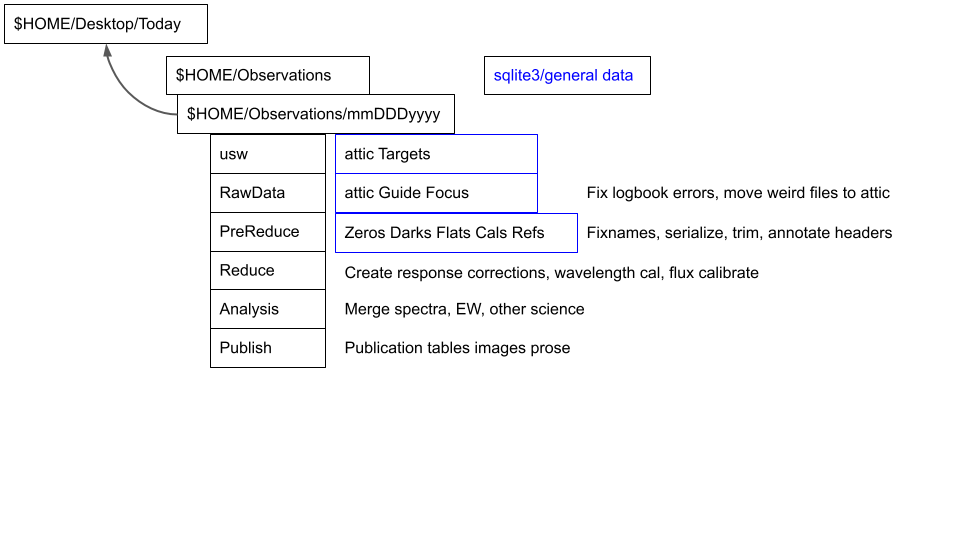
\includegraphics[width=.8\textwidth]{images/Overview1.png}
\caption{Basic Pipeline Steps} %% \caption{{\tiny{citation}}}
\label{figure:basicpipeline}
\end{figure}

\clearpage

\setcounter{section}{0}

\ifx\documentisdraft\drafttest
\linenumbers    %%%%%%%%%%%%% DRAFT
\fi

\clearpage
\pagenumbering{arabic}
%% \fancyfoot[ELF,OLF]{Go to: \hyperref[sec:contents]{Contents}}
%% \fancyfoot[ERF,ORF]{Go to: \hyperref[sec:index]{Index}}
%% \fancyfoot[ECF,OCF]{Page \thepage}

\fancyfoot[LF,OLF]{Go to: \hyperref[sec:contents]{Contents}}
\fancyfoot[RF,ORF]{Go to: \hyperref[sec:index]{Index}}
\fancyfoot[CF,OCF]{Page \thepage}


\section*{Overview}

This document refers to the new IRAF/Pyraf Noirlab 2.18 supported
Pyraf3 : \url{https://iraf.noirlab.edu/} and
\url{https://github.com/iraf-community/pyraf}.

The document covers details system setup for observing and reduction.
We are using a Raspberry Pi/libindi/Ekos for managing cameras and
other details. Once data is captured it is quickly copied to a more
stable platform for backup and reduction. We have IRAF/PyRAF installed
on the RPi to facilitate focus and quick tests of the images.

IRAF/PyRAF is considered a terminal based ``command line
environment'', a very flexible way to use small programs to achieve
large goals. GUI environments restrict users to 'canned' logic. Many
people are uncomfortable with command line work. It requires learning,
practice, and frequent use to maintain a fine edge needed for scientific
data reduction.

This \dhl{Bon Mots} document represents many tricks that one may use
to avoid editing temporary files by hand and to provide an audit trail
for projects.

Go to Section \ref{sec:complexexample} and briefly ponder the code with an
eye towards: ``What is this person thinking!''.

\section{Typography} \label{sec:Typography}

The typographic conventions used in these notes.

Here \llbox{k} means hit the ``k'' on the keyboard. 

\subsection*{Text}

The document uses \dhl{color} to make something \dhl{interesting},
stand out from the text.

\subsection*{Examples}

Examples, in general, state a \dhl{Goal}, the statement of the
\dhl{example}, and \dhl{Prose} to describe the 'thought model' or a
statement about takeaways from the example, and where needed some
exercises. These are presented in this format:

\begin{quote}
\goal Demonstrate a goal. Yes this example was a goal.\\ \example Give
an example of some syntax.\\ \prose Hey, put a linguistic pattern into
your ``thought process'' for that syntax.\\ \exercise[-a] Pick up your
pencil and start your notebook! \\ \exercise[-b] Time to stand for a
minute. \\ \takeaway Tie the thought process to a concrete goal and
example and begin documenting and checking your work.
\end{quote}

\subsection{Margin Annotations}

There are places in the notes where margin annotations are used
to draw attention to something important. In some cases this will
be a note to the author to add/clarify a section of text. Usually
more information may be found in the End Notes section of the document.
\ltodo{Example of Margin Note}{Added a note to demonstrate the note process.}

\subsection{Index}

This document is written in \LaTeX. The \LaTeX environment permits developing
and maintaining a set of bibliographic references, a great index and glossary. 

\section{The Unix and the Data ``Big Picture''}

This document is centered around the Ubuntu 22.04 LTS release using
the NOIRlab IRAF/PyRAF 2.18 pagkage. It offers a paradigm developed
over years of working with IRAF. This leverages Unix. The astronomy
community uses Apple Mac computers that still retain enough about Unix
to allow easy porting of IRAF and friends to that platform, even the
Apple Mx processors.

Win1X requires a VirtualBox (the Microsoft HyperV does not work well
enough).  The client operating system installed in the Virtual box may
be Fedora (the community version of Red Hat Enterprise Linux or RHEL).
This allows installing ESO packages that leverage the RHEL environment.
\textbf{Note}: Some AMD processors will not run hypervisors.
\index(RHEL!ESO) \index{RHEL!Win1X} \index(VirtualBox)

In Unix everything is a 'file'. Programs should be small, perform a
duty and do it well, permit some options. A program takes input from
``standard-in'' (\dhl{stdin}), does its work and puts its output to
``standard-out'' (\dhl{stdout}). Any errrors are reported via
``standard-err'' (\dhl{stderr}). Unix uses a device called a \dhl{pipe}
to send the output from one program into the stdin input of another.
Thus programs can be linked together on one line. 

OK, some programs are huge, and this paradigm does not necessarily
apply. But all the basic Unix utility programs like \dhl{ls}, \dhl{find},
\dhl{grep} etc work this way.

Changing from a GUI paradigm to a command line paradigm is one of the
hardest things for many reading these notes to do.

The Unix philosophy set forth by Ken Thompson, as documented by Doug
McIlroy \cite{McIlroy1978,McIlloryPhilosophy}:

\begin{quote}
Make each program do one thing well. To do a new job, build afresh
rather than complicate old programs by adding new "features". Expect
the output of every program to become the input to another, as yet
unknown, program. -- McIlroy
\end{quote}

GIUs are monolithic in design.\footnote{A GUI is a great way to encapsulate
a process where variation in the process is shuned and discouraged. Scientific
data is noisy and physics is opinionated -- this requires a careful attention
to detail not managable with GUI environments.}

One negotiates with Linux's root process to connect to the Linux
system, where the login process drops the user into a \dhl{shell}. There are
several shells to choose from -- here we will stick with \dhl{bash}
\index{bash}. \textbf{\emph{Note:}} \dhl{/usr/sh} defaults to an abbreviated shell
called \dhl{dash} on most Debian systems. \index{Unix Shell!intro}

\begin{quote}
``On a UNIX system, everything is a file; if something is not a file, it is a process.'' --
Machtelt Garrels, ``Introduction To Linux: A Hands On Guide''
\end{quote}

Peter Freeman \cite{freeman1975software} offered a model of a computer
(and a good operating system) as one of a \dhl{Processor},
\dhl{Memory} and \dhl{Transducer} (PMT) \index{computer!PMT}. The
processors today have less than one core to multiple cores, symmetric
arrays of cores and massively parallel cores.  Even the core of yore
is being supplanted by compute engines, the current popular one is the
GPU with $10^{\$}$ tiny cores.

Files are specialized and fall into classifications like: directories,
special files, links, sockets, named pipes.

There is only one file system and it starts at ``/'' or \dhl{root}.
We tend to think of files as residing on a disk drive. Multiple
drives, and their multiple partitions are simply ``mounted'' at
a location under the ``/''   root directory. Examples are
usually called something like /usr2. Disks on other machines
are usually found, conceptually as a sub-directory the /mnt directory.

\subsection*{The Shell ,``commands'', and Scripts}

The computer sees typed text as groups of characters separated by some
delimiter. Usually the delimiter is a combination of one or more
spaces and/or tab characters. These are called \dhl{whitespace}.

So all of programming takes a stream of complex symbols that, when
taken together, direct the computer to take some safe action. Linux
uses whitespace to set apart each symbol. 

Commands are designed to be typed at the keyboard and are usually
highly abbreviated. One of the handiest commands is \dhl{man}.

\example Use the ``\dhl{man}'' command \\
\prose Hey, what does the man (or ls or ln) command do?\\
\exercise Enter ``\dhl{man man}'' at the shell prompt.\\
\takeaway Read about how man works!\\
\exercise[-b] Enter ``\dhl{man ls}'' at the shell promot.\\
\takeaway Note: it says ``list directory contents'' so the abbreviation
of ``ls'' makes sense. It also offers up a myriad of options.\\
\exercise[-c] Try ``\dhl{ls -l}'' to see details of each file, one per line.\\
\takeaway A way to determine if files are normal files, directories or
links.

One of the oldest Unix commands is ``ls'' used to 'LiSt' directories and
their contents in interesting ways.

\section{Files and Directory Structure}

IRAF/PyRAF 2.18 is installed at a system level, and customized for each user.
The \dhl{mkiraf} command will create a {\textasciitilde}/.iraf directory.

IRAF uses two key files: \dhl{login.cl} and \dhl{loginuser.cl} to select from a myrid
of options and packages one will use for the tasks at hand. The \dhl{login.cl}
file now resides at \dhl{/etc/iraf/login.cl}. The loginuser.cl is located
at {\textasciitilde}/.iraf.loginuser.cl -- this is the file you change.
\textbf{\emph{Note}}: a single line with the word ``keep'' is required at the bottom
of this file.

The loginuser.cl file may be used to add your own special on-off commands,
and to leverage \dhl{foreign} tasks (usually other handy programs on the
path). \index{IRAF!foreign tasks}

Each IRAF task has a set of parameters, managed in the {\textasciitilde}/.iraf/uparam
directory. 

\textbf{BEWARE}: IRAF tasks are ``sticky''. When you change something it remembers the new
thing. The IRAF command \dhl{unlearn <task>} will cause the task to revert to
its defaults. \index{IRAF!sticky}

Other files:

\vspace{-.15cm}
\begin{enumerate}\addtolength{\itemsep}{-0.5\baselineskip}
%\setcounter{enumi}{N}
   \item  {\textasciitilde}/.bashrc, include your own {\textasciitilde}/.iraf-aliases
   \item  login.cl  - traditional configuration, don't edit this one.
   \item  loginuser.cl - configuration to users special taste.
   \item  pyraflogin.py - while not official has handy python functions
   \item  home\$/uparm - where the system keeps parameter files.
\end{enumerate}

\subsection{Directory Layout}

There are two quintessential things about data: 1) preserve the data
and 2) be able to audit processing of the data.

The most important thing is the preservation of the data. Backup,
Backup and Backup again. Then make a copy. It is best to save data on
multiple machines, or to the cloud. Google Drive (and other places)
offer 5TB of data storage for a quite reasonable fee.

All camera data consists of \dhl{16-bit unsigned ADU} values per pixel from
the camera. It is not necessary to change and/or archive raw data with
float values. The QHY600M images are 9600 x 6433 x 2 bytes of image,
roughly 13e6 bytes. Therefore 5TB of disk space will hold roughly
380,000 images. At 3 images per minute for an 8 hour night you get
2400 days of observations for 5TB of disk storage. That's 12 years in
practical terms. However, transferring these images over the net is a
problem.

% (iv (setq tmp (* 9600 6433 2)))    123513600  
% (iv (setq tmp (/ 5e12 13e6 )))    384615
% (iv (setq tmp (/ 384615 (/ 1440 3 3) 200 )))   12     2403

The \dhl{{\textasciitilde}/Desktop} directory allows software acquisiton software to be
configured once. Each night should be copied and archived. 

\begin{quote}
\begin{figure}[h!]
\dirtree{%
.1 {/home/user}.
.2 Observations.
.3 usw  - target lists, cl, notes, other generic things.
.3 ddMMMyyyy  - Date of sunset at Observatory.
.4 usw  - target lists, cl, notes, other generic things.
.4 RawData  - data: warts, blisters and all made read only.
.4 PreReduce  - copy RawData, and work here.
.4 PreAnalysis - pick up analysis for files.
.4 Reduce - Major IRAF/NonIraf reduction.
.4 Analysis - Major IRAF/NonIraf analysis.
.2 Desktop.
.3 Today - where all ``tonights'' observations go.
}
\label{figure:dirlayout}
\end{figure}
\end{quote}


The directory \dhl{usw} is used in lieu of etc. It is the German language
way of saying the samething - \dhl{und so wieder} ``and so again''.
In Unix \dhl{etc} contains loosely related information. For example
puruse \dhl{/etc}, where the system keeps configuration information
of a global level. It is so overloaded something unique is desired.

With this layout, the \dhl{{\textasciitilde}/Observations/usw}
directory contains side files of importance your overall personal
observing strategy. Files, like ds9 region files, special catalog
files general tools etc are stored here. Make subdirectories that
hold common information for different sites or instruments. Copy
those data into a nightly structure as needed.

Data is taken at night. Use dates that reflect the date of sunset
at the site where the data were obtained.

Using the KStars/Ekos/libindi, running on a Raspberry Pi for example,
or a local machine you may want a \dhl{{\textasciitilde}/Desktop/Today} directory
for each night's observing run. In this way the capture/observatory
software does not have to be configured each night. That export directory
remains the same. At the end of the night, simply rename the directory.

Date formats may be confusing, and subject to a computer's LOCALE
subsystem Nobody can make their minds up about date formats.

\centerline{{\huge{{\color{darkred}{SO! SPELL THE DATE OUT!}}}}}

The \dhl{ddMMMyyyy} directory uses the 1 or 2 digit day of month,
followed by the text abbreviation of the month, followed by a 4-digit
year (lets don't play Y2K again). 

This format makes the shell's text completion a quick way to move around.
Text completion involves typing a few starter characters of the file/directory
name then hit the tab. It will advance to the next non-unique thing.

Underneath \dhl{ddMMMyyyy} is the usw directory for tonight's work. The
target list, special catalog file of reference stars etc, the scheduler's
input. Here we store the \dhl{reduce.cl} or \dhl{reduce.py} script
template to be developed for these particular data.

The RawData/PreReduce/PreAnalysis/Reduce/Analysis directories are
cascading stages of data. You may use an \dhl{attic} directory where
to sideline unrelated or terrible images.

You can automate file reduction by using sub-scripts/tasks within the
melange of IRAF/PyRAF/bash/python/whatever language programs and then
leveraging Python and cl into making a
\dhl{OBSERVATION/usw/reduce.pyraf}\index{reduce.cl}
script\index{reduce.pyraf} script for the data. Save this as a template in
the general \dhl{usw} directory, and copy in to each observation's repository.
Detailed example is in Appendix \ref{sec:ReducePyrafControlFile}.

At this time PyRAF (a mix of ecl and Python) does not act well as a
``script'' due to the hack that adds ecl syntax to the GNU runline command
input. It uses the raw input directly and side-steps \dhl{stdin}. This
violates the Unix philosophy of each program should take its input from
stdin, process its results and put the results into stdout.  This
allows one to pipe programs together to achieve an ultimate goal.

Scripts may be written in the \dhl{.cl} language (really ecl or extended cl),
actual PyRAF (\dhl{.pyraf}), or hacked into PyRAF with the \llbox{!}
cl prefix as you go along.

\textbf{\emph{Note}}: The \dhl{.pyraf} scripts blend python and PyRAF together.
See the complicated example of how to deal with APO NICFPS camera
images.

\section{Critical First Steps}

It is critical you properly install the IRAF/PyRAF3 packages. This
release looks for a {\textasciitilde}/.iraf directory that may not be fully integrated
into the rest of IRAF.

You may make a soft link of \dhl{\home/iraf} to \dhl{\home/.iraf}:

\dhl{ln -s \home/iraf \home/.iraf}

The document will continue to refer to \dhl{\home/iraf} as the base
of the IRAF package. 

It is important to use a \dhl{~/iraf/loginuser.cl} file with task
aliases foreign and tasks.\index{tasks!aliases} \index{tasks!foreign
  tasks}

One way to make things simple is to create a bash alias for pyraf that:
\vspace{-.15cm}
\begin{enumerate}\addtolength{\itemsep}{-0.5\baselineskip}
%\setcounter{enumi}{N}
   \item   uses xdotool to change the color of the window's background
   \item   update the PATH and PYTHONPATH to access all the special files you use
   \item   run the system pyraf (note the /usr/bin path is prefix is necessary) 
 with the ``-s'' switch for ``silent'' start.
\end{enumerate}


\begingroup \fontsize{10pt}{10pt}
\selectfont
%%\begin{Verbatim} [commandchars=\\\{\}]
\begin{verbatim} 
alias pyraf="xdotool key shift+F10 r 1;\\
  export PATH="/usr/local/bin:$PATH"; export PATH="/usr/local/astrometry/bin:$PATH";\\
  export PYTHONPATH=$HOME/.iraf; export PATH="$HOME/.iraf/smtsci/bin:$PATH";\\
  /usr/bin/pyraf -s;"
\end{verbatim}
\endgroup
%% \end{Verbatim}

\subsection{IRAF/PyRAF Tasks and Packages}

IRAF, from ye-olden times, uses \dhl{packages} containing help text
and parameter files to hold values from run-to-run together with the tasks'
executable code.
\index{IRAF!tasks} Tasks are ``programs'', usually written in FORTRAN
or in cl proceedural code. Some are written in C/C++.

\dhl{BEWARE}: IRAF is \dhl{sticky}! It retains parameter values from
run-to-run that can perpetuate errors. Review all the parameters to be
sure your reductions are proper. These values are stored in the
\dhl{~/iraf/uparm} directory.

Tasks are built into IRAF/PyRAF but are only loaded once. Each time
they are used -- they are in memory and already part of the CPU thread
you are using. Thus they very fast. Using \llbox{!} shell-escape or a
\dhl{\$foreign} task causes Unix to create a new heavy-thread with
significant overhead (especially in a loop).

IRAF has a habit of loading images into memory and keeping them there.
Some tasks will modify the in-memory image but not write it back to
the disk. Work may be lost. See Section \ref{sec:FITSFiles} for quick
details.

IRAF has a neurotic habit of \dhl{sometimes} adding an extent to
certain FITS files! This is the case with master darks and flats
and a handful of other operations.

It is best to develop your \dhl{reduce.pyraf} script in an editor, one line
and step at a time, then cut/paste edited lines at the interactive
prompt. When you make a mistake -- and you will -- you can start over
with a fresh copy of data and stop short of the mistake. Pick up and
go again.

\subsection{Full On Python Hacks}

\example Python's \dhl{import iraf} statement allows for operations like: \\
\prose I want to use IRAF's imstat command to get a binary value, assign
the value to my python variable. \\
\exercise Enter: \\
{\color{verbcolor}{
\begingroup \fontsize{10pt}{10pt}
\selectfont
%%\begin{Verbatim} [commandchars=\\\{\}]
\begin{verbatim} 
mymean = float( iraf.imstat(images='*fits',fields='mean',format=iraf.no,Stdout=1)[0])
\end{verbatim}
\endgroup
%% \end{Verbatim}
}}

\takeaway The task has a pythonic wrapper, contained in the iraf.py
module's namespace.  It needs a list of files, we only want the one
field \dhl{mean}, we do not want the headers (format=iraf.no). The
phrase Stdout=1 (note capitalization) returns the text as a string
rather than printing on the terminal. But! The string is actually an
array, so we want the first bit. But! that bit is a string, and we
need to convert to binary with the \dhl{float} python function.

where \dhl{mymean} is now a proper python float. Yes, convoluted, but
its buried in a scrip and available for your use. \index{Stdout}

\subsection{Task Parameters}

Always be aware of the:
\vspace{-.15cm}
\begin{enumerate}\addtolength{\itemsep}{-0.5\baselineskip}
%\setcounter{enumi}{N}
   \item    ~/iraf/uparm directory
   \item    lparm <taskname> command to list parameters.
   \item    \dhl{unlearn <task>} command.
   \item   help <task> and look at the see also part at the bottom.
\end{enumerate}

\section{Goals}

The main goal of scripting is not the script, it is the result. Good
data results do not come from good scripting -- but come from good
planning, good execution of the plan and attention to configuring
your tools.


\subsection{Things to remember}

IRAF \dhl{cl} morphed into PyRAF \cite{2006hstc.conf..437G} to allow a more
powerful \dhl{cl} by hacking the Python \dhl{readline} subsystem. The
grammar of python was altered to allow for a ``direct entry'' of most older
\dhl{cl} commands. Direct access to the underlying tasks was
accomplished with a ``cythonic'' interface into underlying code. An ``iraf''
module was added to support programming calls to IRAF tasks and using 
a special Python \dhl{keyword} argument Stdout to return output as a string.
Parsing this string with python allows chaining \dhl{cl} commands together
for a goal.

A tremendous amount of power is available for you to mix and match to meet
your specific needs. 

\subsection{Observation Directory}

One can not expect proper structure by simply importing a night's
observations, warts blisters and all. Files will be scattered all
over, mis-named, bad headers, useless(!), and other oddities. But copy
the data into date/RawData. See directory layout table \ref{figure:dirlayout}

Open date/usw/reduce.cl in your favorite editor. Anything you want
to type into PyRAF -- type it into the reduce.cl file. Then cut/paste
the command to PyRAF. This means when you make the mistake -- you
can remove the last line, save the reduce.cl file, and rebuild
to that point. Yes, some interactive things will or may happen.
Try not to make too many mistakes.

\vspace{-.15cm}
\begin{enumerate}\addtolength{\itemsep}{-0.5\baselineskip}
   \item   cd ~/Observations
   \item   mkdir 22Feb2022 \# date of sunset at the observatory
   \item   cd 22Feb2022
   \item   mkdir -p Plan RawData PreAnalysis Analysis Publish usw
   \item   mkdir -p PreAnalysis/{Bias,Darks/{s300,s3},Flats,Comps} \# prior knowledge
   \item   cd RawData
   \item   cp -pr /mnt/NAS/22Feb2022/* .  \# copy the raw data
\end{enumerate}

Now the plan for observations and initial PreAnalysis results is in 
place. The \dhl{usw/reduce.cl} script is the key. 

Good observations are the result of good planning. Make the list of targets,
determine offsets and guide stars, create a ds9 region file in ICRF WCS
coordinates for the field of view and possible orientations of the instrument.
If possible download the preparation package from the observatory and take
time to prepare. \index{planning}

\begin{figure}[h!]
\centering
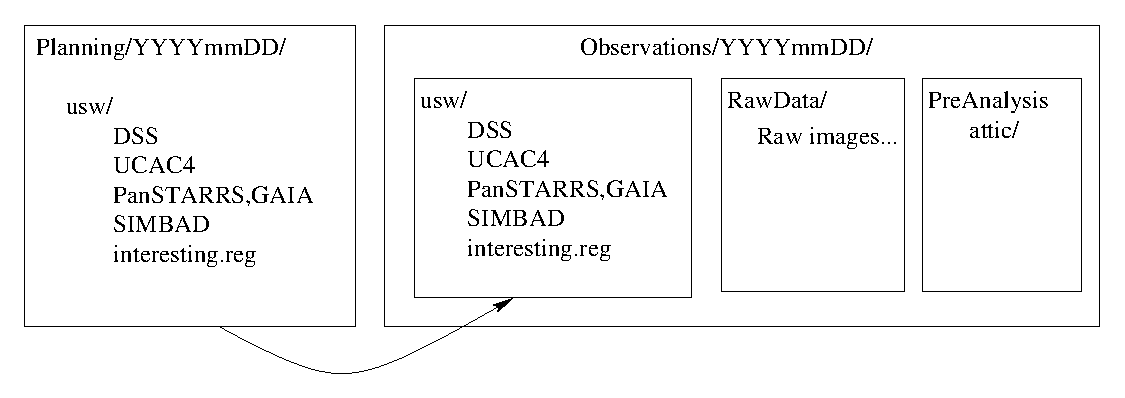
\includegraphics[width=.4\textwidth]{images/Overview.eps}
\caption{The observations directory was in place with the plan.
Load up the raw images. Then copy raw data to pre-analysis.} %% \caption{{\tiny{citation}}}
\label{figure:GoalsOverview}
\end{figure}

\clearpage
\subsection{The main tricks}

Note: Unix files do not rely on their extensions. A Unix extension is a social
convention. Many authors use two files, like \dhl{in.txt} and \dhl{out.txt}.
They will use an editor to change the bits of one to another. 

I recommend using goofy file names, like \dhl{xxx} and \dhl{l.l}, when seen
they may be removed. The filename \dhl{l.l} is real easy to type because
the \llbox{l} and \llbox{.} are right next to each other!

The \llbox{/}\llbox{/} sequence is the cl concatenation operator, used to
join two strings without intervening whitespace.

Instead of having the input files in in.txt, then editing to make unique
output names -- simply prepend a string, with some meaningful context
to the @file. 

The order of operations may be to
\vspace{-.15cm}
\begin{enumerate}\addtolength{\itemsep}{-0.5\baselineskip}
%\setcounter{enumi}{N}
   \item   t\_ trim a file.
   \item   c\_ cosmic ray removal
   \item   z\_ to zero correct
   \item   d\_ to dark correct
   \item   f\_ to flat a file
\end{enumerate}


etc. data.fits, after processing may be \dhl{f\_d\_z\_c\_t\_data.fits}.

So PyRAF has several tricks up its sleave:
\begin{itemize}
\addtolength{\itemsep}{-0.5\baselineskip}
   \item   It can act like a basic ``calculator'' just by typing standard python at the
PyRAF command prompt. Remember to ``import'' packages like math and numpy.
   \item It works with list of files. These are refered to as ``list''
     or ``at'' files. They are like {\color{verbcolor}{\verb#@l.l#}}
     where the file ``l.l'' has a list of filenames -- one per line.
   \item You can take the files in ``l.l'' and produce new files with
     the same name but prepend a clause to the
     filename!\\ \textbf{E.g.:}
     {\color{verbcolor}{\verb#imarith @l.l - zmaster.fits z_//@l.l#}}\\ will
     subtract the zero master from each file in ``l.l'' and make a
     corresponding {\color{verbcolor}{\verb#z_filename.fits#}}.
\item PyRAF is a a replacement for {\color{verbcolor}{\verb#cl#}} (actually
ecl). You can loop {\color{verbcolor}{\verb#.cl#}} commands together
with bash commands into the mix to do work using:\\
{\color{verbcolor}{\verb#cl < ~/iraf/fit2fits.cl#}} to bring a Vendor's
fit format to the PyRAF standards.
\end{itemize}

It has a few oddities, inherited from the ecl lashup of the Pythonic 'readline' hack,
ripped from a \dhl{reduce.cl} script:

\vspace{-.15cm}
\begin{enumerate}\addtolength{\itemsep}{-0.5\baselineskip}
   \item Oops! Its Python 2.7 so write helpers like \dhl{trim} and
     \dhl{fitsls} accordingly.
   \item   Most of the IRAF \dhl{cl} commands work
   \item   \dhl{set OBSROOT=/home/me/Observations/23Feb2022}
   \item   \dhl{set OBS=OBSROOT\$/PreAnalysis}
\end{enumerate}

The IRAF command \dhl{chdir} \index{cl!chdir} changes directory while respecting
the IRAF use of iraf-environment variables.

You can escape to bash by starting the line with a bang (!). This
allows developing handy bash scripts to store in iraf/bin.

\clearpage

\subsection{System Setup}

I presume the use of the Ubuntu 22.04 Linux distribution from Canonical\texttrademark.

%% Under Microsoft Windows\texttrademark Pro, there is a system called \dhl{Hyper-V}.
%% It is very ``light-weight'' virtualization layer for Windows that permits
%% the seamless of an essentially containerized Ubuntu 22.04 + anaconda and other
%% Linux based tools while maintaining contact with the Windows file system,
%% the network etc. \index{Windows!Hyper-V}.

%%Under Linux you are running Linux anyway.
MacOS is very Linux like, even on their M1 processor series.

Install the Anaconda package without the Navigator. This brings in
a massive amount of power, including Astropy \cite{astropy:2013} \cite{astropy:2018}
\cite{astropy:2022}.
\vspace{-.15cm}
\begin{enumerate}\addtolength{\itemsep}{-0.5\baselineskip}
   \item    Necessary:
\vspace{-.15cm}
\begin{enumerate}\addtolength{\itemsep}{-0.5\baselineskip}
   \item    Ubuntu 22.04/Mac OS + many apt-get packages
   \item    Anaconda (Python 3+)
   \item    Astroconda PyRAF recipe (a python2.7 env)
   \item    Ubuntu aptitude iraf/pyraf packages
   \item    Sextractor
   \item    Current SAOImage/ds9
   \item    Current Astrometry.net + 4200 and GIAI data
   \item    Fitsverify \cite{fitsverify-1}
   \item    GitHUB sasiraf package (currently private contact author.)
\end{enumerate}
   \item    Optional
\end{enumerate}

\subsection{Unix\texttrademark Aliases}
A few aliases need to be setup.

\ltodo{Add Aliases}{Update/add aliases for bashrc file.}

\begin{figure}
{\color{darkred}
\begingroup \fontsize{10pt}{10pt}
\selectfont
%%\begin{Verbatim} [commandchars=\\\{\}]
\begin{verbatim} 
function pyraf  { #export PYTHONPATH=$HOME/iraf;
                  export PATH="/home/wayne/anaconda3.8/envs/geminiconda \\
                     /bin:$HOME/iraf/smtsci/bin:$PATH"; (folded line)
                  source activate geminiconda;
                  xdotool key shift+F10 r 6;     # change terminal color
                  $HOME/anaconda3/envs/geminiconda/bin/pyraf -s $*;
                }
\end{verbatim}
\endgroup
%% \end{Verbatim}
}
\caption{An entry into the aliases file, using the Gemini pyraf installation.}
\label{fig:geminialias}
\end{figure}

This is a little-bit complicated:
\vspace{-.15cm}
\begin{enumerate}\addtolength{\itemsep}{-0.5\baselineskip}
   \item   The PYTHONPATH allows pyraflogin3 to be imported after start.
   \item   This assumes \dhl{~/iraf/pyraflogin.py} is present.
   \item   The function in figure \ref{fig:geminialias} tells Anaconda to activate
     the geminiconda environment
   \item   The xdotool allows the color of the terminal window to be changed.
   \item   PyRAF is then started, the \dhl{-s} switch is quiet about packages loaded.
   \item When pyraf starts, it loads \dhl{login.cl} which in turn
     loads my \dhl{loginuser.cl} scripts.
\end{enumerate}

\subsection{Initialization files}

PyRAF uses \dhl{~/.iraf/login.cl} to manage system level commands and should
not be edited -- except to ensure that \dhl{cl < "home\$/iraf/loginuser.cl"} is
enabled. Edit the \dhl{loginuser.cl} file and pile changes.
 \index{Initialization!login.cl}
\index{Initialization!loginuser.cl}

A special \dhl{~/iraf/pyraflogin.py} file can 'extend' the Python
environment.  A sample file is available with this package. It
requires the special alias to start PyRAF. It adds simple
\dhl{matplotlib} plotting and some handy fixer-upper functions. See
that package for documentation. \index{Initialization!pyraflogin.py}

\subsection{Initial Steps}

This process uses a user-defined  directory structure as shown in
figure \ref{figure:basicpipeline}. 

The main steps are:
\vspace{-.15cm}
\begin{enumerate}\addtolength{\itemsep}{-0.5\baselineskip}
   \item   Layout basic directory structure:


   \item  Add a few toplevel soft-links for non-sentient file browsers.
\dirtree{%
.1 \$HOME/.aaatoday linked to \$HOME/Desktop/Today.
.1 \$HOME/.aaareduce linked to current working reduction.
}

   \item   Planning - load up the \dhl{\$HOME/Desktop/Today/usw} directory with
FOV files, and anything related to observatory etc.

   \item   Observe
   \item   Move dhl{\$HOME/Desktop/Today} to dhl{\$HOME/Desktop/Observations/mmDDDyyy}
date of sunset at the observatory of the instrument.
   \item   Make a safe backup.
   \item   Start the process of reducing the data.
\end{enumerate}

The script provides the audit trail you used. Modify this for each
instrument setup, and for each filter type etc.  Essentially the same
for spectroscopy -- just watch the statistics sections.

You may not need darks, and the flats will be different.

When, not if, you mess up you can delete the PreAnalysis directory, fix
the above script, and start over. As you move deeper into the file
processing, the script becomes more valuable.


\clearpage
\subsection{PyRAF Calculator Mode}

\goal Demonstrate borrow Pyraf as a calculator within PyRAF. Determine
the mean plus 3 times the standard deviation for a limit.

\example 
{\color{verbcolor}{\verb#imstat zmaster.fits fields=mean,stddev#}} \\
you find the mean is 346 and the stddev is 47.

\exercise How many pixels in the zero master are 3 or 5 $\sigma$ above
the mean?

{\color{verbcolor}
\begingroup \fontsize{10pt}{10pt}
\selectfont
%%\begin{Verbatim} [commandchars=\\\{\}]
\begin{verbatim}
from astropy import fits  # DO THE IMPORTS ONCE
import numpy

f = fits.open('zmaster.fits')    # open the fits file as a cfitsio like
d = f[0].data   # get the data   # structure and just grab the data.
# using some python magic!
(mean,stddev) = map(float,
                   iraf.imstatistics(Stdout=1,fields='mean,stddev',
                      images='zmaster.fits',format=iraf.no)[0].split())
len(d[d> mean + 3.0*(stddev)]) # 25729 pixels matched this example
len(d[d> mean + 5.0*(stddev)]) #  1220 pixels matched this example
f.close()
\end{verbatim}
\endgroup
%% \end{Verbatim}
}


\prose Hey, we're PyRAF, a pythonic interpreter -- so lets really use
Python.  The imports are used to get the modules/functions we
need. The fits.open gets the FITS file open for business; we grab just
the image data as a numpy array of shape
{\color{verbcolor}{\verb#NAXIS2,NAXIS1#}} (switched(!), numbered from
zero now and the data will have overscans if present!) using
{\color{verbcolor}{\verb#d = f[0].data#}}. The
{\color{verbcolor}{\verb#iraf#}} is imported by virtue of we're PyRAF;
the {\color{verbcolor}{\verb#imstat#}} is run as a python function
using {\color{verbcolor}{\verb#iraf.statistics()#}}.  The
{\color{verbcolor}{\verb#Stdout=1#}} tells the task to return the
output not send it to the terminal. The
{\color{verbcolor}{\verb#format=no#}} tells the function to omit the
usual header text etc, and just return the two values requested with
the {\color{verbcolor}{\verb#fields="mean,stddev"#}}.  The output is
one string with two ASCII numbers. These are split into an array, then
the {\color{verbcolor}{\verb#float#}} function converts the strings
into actual numbers -- returned as the tuple
{\color{verbcolor}{\verb#(mean,stddev)#}}.

\subsection{Using Numpy Arrays}
%HEREHEREHERE

Numpy arrays follow the ``C'' indexing scheme, which is ``ordinal'' in nature
(starting with zero). For an (X,Y,Z) index -- the array is referenced \dhl{backwards}:
myarray[Z][Y][X]. This differs from the FORTRAN convention for arrays, ``cardinal''
in nature (counting from 1).

FITS images are stored in FORTRAN order, and in Big Endian format. This makes
difficult for Intel architectures.

This is critical. Data are written into FITS images in so-called \dhl{Big-Endian}
fashion. In Jonathan's ``Gulliver's Travels'', a fictional character encounters
a culture in heated conflict over weather or not one should crack open an
egg on the little end or the big end. Computer aritectures are conflicted on
how to store a larger value, say an integer that spans more than one byte
into a linear address space. Decisions (bad perhaps) were made to store
a 16-bit integer with the byte containing least significant digit first.
The word oxBO is stored with the 0 first then the 0x0B. This was to make
a very early machine fast at ++value operations! We're stuck with that decision
since.

The real issue boils down to the Bad Thing\texttrademark practice of
``type punning'' whereby a block of data in ``Endianess Be Damed''
format is read into memory, then attempts to access it as though it
had the right byte order results in catastropy when data is exchanged
between the types of architectures.

Intel processors are ``Little Endian'' where processors like the Motorla
68000 were ``Big Endian''. 

Data are stored as arrays, with astropy.fits.io open command setting the
data[0] extent as a pythonic numpy array. So the indices are a bit backwards
The fits header would read something like:

\begingroup \fontsize{10pt}{10pt}
\selectfont
%%\begin{Verbatim} [commandchars=\\\{\}]
\begin{verbatim} 
NAXIS  = 2
NAXIS1 = 2048
NAXIS2 = 512
\end{verbatim}
\endgroup
%% \end{Verbatim}

To store a 2D image array. This is ment to denote an image that is 2048 wide and 512
tall. 

\ltodo{numpy vs FORTRAN}{Get into index details.}


The next bits use numpy arrays. Here we use the conditonal indexing
mode common to numpy arrays to get all the pixels that match
expression of the value > the
{\color{verbcolor}{\verb#mean + n times stddev#}}.

Need a ``Quick Calculation'' to find the center of an image to
use as a ``statistics section'' for normalizing?:

{\color{verbcolor}
\begingroup \fontsize{10pt}{10pt}
\selectfont
%%\begin{Verbatim} [commandchars=\\\{\}]
\begin{verbatim}
imhead zmaster.fits   # result is 'zmaster.fits[1368,1364][real]:'
# half size? pick up the [NAXIS1,NAXIS2] from abbreviated imhead result...
(1368//2, 1364//2)   # returns tuple (684, 682)  the '//' is integer divide.
print "[%d:%d,%d:%d]" % (1368//2 - 50, 1368//2 + 50, 1364//2 - 50, 1364//2 + 50)
# [634:734,632:732]  Et Viola! A handy center stat section for normalizing!
\end{verbatim}
\endgroup
%% \end{Verbatim}
}

Make your own functions! Then imexamine -- the comp star and the target star.

{\color{verbcolor}
\begingroup \fontsize{10pt}{10pt}
\selectfont
%%\begin{Verbatim} [commandchars=\\\{\}]
\begin{verbatim}
import math    # DO THIS ONCE
def mag(compmag,compflux,observedflux):
   return -2.5(math.log10(observedflux / compflux) + compmag
\end{verbatim}
\endgroup
%% \end{Verbatim}
}

\exercise Correct for background.

\section{Getting Started}

Configure the system. Copy the login.cl to ~/.iraf. Copy loginuser.cl script
to ~/iraf. \textbf{\emph{Note}} One has a hidden-file dot.

Add the .iraf.aliases file to \dhl{\$HOME} directory and if you like, add it to
the \dhl{\$HOME/.bashrc} file.

Start PyRAF in one window and start Editor in another window. I
recommend emacs or Sublime Text as editors -- they are GUI
oriented. Remember all things have a learning curve.

Why we use the vi editor. Vi is the ``\dhl{Vi}sual Editor'' that sits
on top of a powerful albeit basic Unix editor ``\dhl{ed}. The \dhl{ed}
editor is the basis for the \dhl{sed} the Unix stream editor. Regular
expressions (think wildcards) are very sophisticated and turn up all
over the Linux/Unix system. They are worth the effort to learn. The
``re'' of the grep program (\dhl{g}lobal \dhl{re}gular expression
\dhl{p}rint) program obviously makes heavy use of regular expressions.

The very basic Linux commands are:

\begin{table}[h!]
\centering
\begin{tabular}{| l | l |}
\hline
Command  & Basic Action   \\
\hline
cd    & change directory    \\ 
ls    & list files     \\ 
pwd   & print the current working directory    \\ 
cat   & \dhl{concatenate} file(s)    \\ 
less  & view content of a file    \\ 
man   & the Manual -- print details of a command \\ 
which & show where on PATH an executable is \\ 
rm    & remove files and directories. \\
%% ones-based: \cline{a-b}
\hline
%%\DeleteShortVerb{|}
\end{tabular}
%%\end{minipage}    %% for footnotes  r@{.}l 
\caption{Very Basic Unix Commands}
\label{table:VeryBasicUnixCommands}
%%} % end small etc
\end{table}


\subsection{Very Basic PyRAF commands}

\begin{table}[h!]
\centering
\begin{tabular}{| l | l |}
\hline
Command  & Use   \\
\hline
cl            & run the cl editor                            \\
epar          & edit parameters/launch task                  \\
hedit         & fast/dirty header editor                     \\ 
imhead        & list the header values for a file            \\ 
hselect       & select values from headers                   \\ 
imexamine     & all manor of ways to view images             \\ 
apall         & reduce a spectrum image                      \\ 
identify      & identify spectral lines assign wavelenghts   \\
dispcor       & apply identify results to science spectrum   \\
splot         & view/analyze reduced spectrum                \\ 
imstat        & print mean,min,max,std etc for set of images \\ 
%% ones-based: \cline{a-b}
\hline
%%\DeleteShortVerb{|}
\end{tabular}
%%\end{minipage}    %% for footnotes  r@{.}l 
\caption{Very Basic IRAF/PyRAF commands}
\label{table:VeryBasicIRAF/PyRAFcommands}
%%} % end small etc
\end{table}


\section{Working on subsets of files.}

IRAF uses ``list files'' denoted \dhl{@list.txt}. The \llbox{@} key
as the first character of the filename tells IRAF to open that
file and take from it filenames -- one filename per line. This is
real handy.

Some documents have you make lists, then use an editor to change the
list as you go. They recommend filenames like mylist.txt. This is
cumbersome to type. Try using a simple name like \dhl{l.l}. Note the
\llbox{l} key is very near the \llbox{.} key! Handy to type.  If you
see the file \dhl{l.l} you know you can simply remove it.  The \llbox{!}
as the first character on a command line sends the rest of the line
to the local bash script. This escape mechanism allows you to use
all the power of Unix inside cl scripts.

The command \dhl{!ls -1 *Dar* > l.l} takes all filenames with Dar
in it and lists them out in lexicographical (sorted) order. Here
are some example of ways to build list-files.

{\color{verbcolor}
\begingroup \fontsize{10pt}{10pt}
\selectfont
%%\begin{Verbatim} [commandchars=\\\{\}]
\begin{verbatim}
!ls -1 *fits > l.l
cl < ~/iraf/crall.cl
# all the files are now c_<filename>

hselect c_*fits $I "IMAGETYP ?= 'Bias'"  > l.l
hedit @l.l IMAGETYP zero add+ show- ver- update+
!if test -e zmaster.fits; then rm zmaster.fits; fi  # bash to rm file if exists
imcombine @l.l zmaster.fits combine=median

hselect c_*fits $I IMAGETYP ?= 'Light'"  > l.l
hedit @l.l IMAGETYP object add+ show- ver- update+
imarith @l.l - zmaster.fits z_//@l.l
imarith z_//@l.l - dmaster.fits d_z_//@l.l
imarith d_z_//@l.l / flatmaster_SII.fits f_d_z_//@l.l

# files are now {\color{verbcolor}{\verb#f_d_z_c_filename.fits#}}
\end{verbatim}
\endgroup
%% \end{Verbatim}
}
This makes use of the fact that we can pile on prefixes to
processed files:

\begin{itemize}
\addtolength{\itemsep}{-0.5\baselineskip}
   \item   t - trimmed
   \item   c - cosmic ray reduced
   \item   z - zero subtracted
   \item   d - dark corrected
   \item   f - flat normalized
\end{itemize}

At the end, a flat-normalized file called {\color{verbcolor}{\verb#science.fits#}} will
have the name {\color{verbcolor}{\verb#f_d_z_c_t_science.fits#}}.

Lots of intermediate files lying around: Clean them up!

{\color{verbcolor}
\begingroup \fontsize{10pt}{10pt}
\selectfont
%%\begin{Verbatim} [commandchars=\\\{\}]
\begin{verbatim}
print "Remove residual files."
! (export LC_ALL=C; rm [a-z]_*fits 2> /dev/null;)
\end{verbatim}
\endgroup
%% \end{Verbatim}
}

\textbf{\emph{Prose:}} \textbf{\emph{Hey}} PyRAF send the line to bash; but! using a sub-shell
set {\color{verbcolor}{\verb#export#}} the {\color{verbcolor}{\verb#LC_ALL=C;#}}
shell variable to let bash actually use case sensitive wildcards. Then
{\color{verbcolor}{\verb#rm [a-z]_*fits 2> /dev/null;#}} remove the
file -- and in case there is some whining about the process, send the
whines to the bit-bucket ({\color{verbcolor}{\verb#/dev/null#}}).


\section{Observing}
PyRAF \index{PyRAF!Observing} is a useful tool for spectroscopy. Using
the imexamine command and the 'j' key: set the rplot to wider than a bright
line width. 

% HEREHEREHERE

\clearpage
\section{Overall Philosophical Approach}

This document covers a philosophy --- a set of general tools and
scripts to take and reduce data.

In this case some location like {\color{verbcolor}{\verb#/opt/myobs/iraf/#}}
or {\color{verbcolor}{\verb#~/iraf/#}} contains a number of small generic
{\color{verbcolor}{\verb#.cl#}} scripts to handle specific needs. These
are specific to certain conditions -- like a package that writes {\color{verbcolor}{\verb#.fts#}}
instead of {\color{verbcolor}{\verb#.fits#}} files. Routines to remove pesky
spaces that GUI users like to use; get rid of multiple ``dots''; plus signs
etc. 

\vspace{-.15cm}
\begin{enumerate}\addtolength{\itemsep}{-0.5\baselineskip}
   \item   Create a planning directory. Rename to Observations/directory
when the plan is executed.
   \item   Create a ``usw'' directory to hold the plan, collect pre-analysis information:
\vspace{-.15cm}
\begin{enumerate}\addtolength{\itemsep}{-0.5\baselineskip}
   \item   DSS image -- ds9 Analysis \menu Image Servers
   \item   Region files, catalog files for ds9 -- ds9 Region \menu Shape ...
   \item   Photometry reference stars --- ds9 Analysis \menu Catalogs \menu Database \menu UCAC4;
or with the Aladin application and TOPCAT make one the hard way. (PanSTARRS DR1).
   \item   Bibliographic information -- Browser and SIMBAD for the target(s).
   \item   Gather any existing bad pixel masks -- previous runs; observatory supplied files.
\end{enumerate}

   \item  Gather raw data --- stay up all night
   \item  Archive raw data as a RawData and make read only --- back to your {\color{verbcolor}{\verb#Observations#}} directory:\\
{\color{verbcolor}{\verb#(cd Observations/YYYYmmDD; mkdir -p RawData; cd RawData; rsync <from somewhere> .; chmod -w -R *#}}).
\end{enumerate}


\vspace{-.15cm}
\begin{enumerate}[resume]\addtolength{\itemsep}{-0.5\baselineskip}
   \item   Copy raw data to a PreAnalysis directory -- do not damage any
raw data whatsoever. Make the PreAnalysis files writable:\\
({\color{verbcolor}{\verb#cd Observations/YYYYmmDD; mkdir -p PreAnalysis; cd PreAnalysis; cp -pr ../RawData/* .; chmod +w -R .#}})\\
Clean data and make initial analysis files:
\vspace{-.15cm}
\begin{enumerate}\addtolength{\itemsep}{-0.5\baselineskip}
   \item   Fix the filenames --- {\color{verbcolor}{\verb#cl < ~sbo/iraf/fix_sbig.cl#}}
   \item   Fix the headers--- {\color{verbcolor}{\verb#cl < ~sbo/iraf/fix_headers.cl#}}
   \item   Trim (remember) overscan --- see above
   \item   Remove bad WCS especially from zero/dark/flats {\color{verbcolor}{\verb#cl < ~sbo/iraf/fix_sbig_wcs.cl#}}
   \item   Remove cosmic rays ---  {\color{verbcolor}{\verb#!ls -1 *fits > l.l#}}
followed by {\color{verbcolor}{\verb#cl < ~sbo/iraf/crall.cl#}}
\item Other basic reduction steps to be covered elsewhere:
\begin{enumerate}\addtolength{\itemsep}{-0.5\baselineskip}
   \item   Make any bad pixel masks 
   \item   Make master zeros and darks 
   \item   Make master flats 
   \item   apply zeros,darks,flats to science images
   \item   add new WCS or de-distort and add new WCS
   \item   extract photometry
   \item   combine images for deeper photometry
   \item   freeze this work
\end{enumerate}
\end{enumerate}


   \item  Copy the PreAnalysis data into an Analysis Directory.
(Any damage here is quickly recovered from PreAnalysis.)\\
{\color{verbcolor}{\verb#!(cd ..; mkdir -p Analysis; cd Analysis; cp -pr ../PreAnalysis/f_d_z_c_t* .)#}}
\end{enumerate}


A break down of the above steps reveals the need to make/use
certain scripts (some shown in red in context above):

\vspace{-.15cm}
\begin{enumerate}[resume]\addtolength{\itemsep}{-0.5\baselineskip}
   \item   Fix the filenames: remove dots, spaces, dashes other special characters.
   \item   Fix the headers: Observatory/Vendor non-IRAF keywords to IRAF
keywords; Very-Non-Standard keywords like PCOUNT and GCOUNT
   \item   Pinpoint is good enough for tracking (still takes a while to apply
and will fail) but is not accurate.
   \item   Single Pixel errors from cheap cameras, inevitable cosmic rays need
to be mitigated in raw zero, dark and flat frames.
   \item   Masks provide locations in pixel coordinates of defects that can ruin
the science.
   \item   Adding a new WCS will help to quickly align images. This may be enough
if there is no distortion, de-distort with flux conservation where possible.
\end{enumerate}


You can stop here and defer photometry to the analysis step. However,
you can extract photometry using sextractor and a few tricks.

Combining images is an art.


\textbf{\emph{Main goal:}} to develop a \textbf{\emph{compact}} set of
skills with Unix/Python/PyRAF/IRAF to create a
\textbf{\emph{collection}} of IRAF scripts to process images from two
cameras, three telescopes using vendor's software. In this sense,
``compact'' means: the basic IRAF commands; python, bash and Unix
tricks and commands; a basic use of SAOImage/ds9. A familiarity with
command line operations and vocabulary to support planning, executing,
reducing data and publishing photometic data. Summary: the course is
designed to introduce astrophysical hands-on research -- not the
tedious nature of the related software tools.

Examples, long and short, will provide an overview of all the weird/odd ways
Bash/IRAF/PyRAF and Python are used is in Appendix \ref{app:PutItTogether}.

\textbf{\emph{The Problem:}} PyRAF is a ``pythonic''
wrapper/controller of collection of IRAF tasks/commands that in turn
are based on the Unix operating system. The long path to getting a
handle on PyRAF is to build on knowledge gained over time: starting
with Python, then Unix in general and the bash shell in particular,
then IRAF commands and tasks. This is hard to do in two weeks.

\textbf{\emph{Exercise:}} we'll jump into the middle of the mess and
build as we go. To temper this exercise, examples are from a third
observatory and vendor's software -- this is to
\textbf{\emph{prevent}} a simple cut/paste without taking the time to
understand each fragment of the provided example code.


\section{PyRAF, IRAF and Unix (bash)}

IRAF was developed in a slow rather ad hoc fashion, its birthday
established by Donald Wells \cite{FITSBirthday} as 28 March 1979,
real development started in 1981 and was it put to use in 1984
\cite{1993ASPC...52..173T}.  At the time researchers at various
institutions using various computing platforms developed ``packages''
that were brought together at NOAO under IRAF (Image Reduction and
Analysis Facility). It was developed under Digital Equipment
Corporation's PDP and Vax computing environments as well as Unix. The
result today reflects coding and use patterns in vogue since that
time. \index{IRAF!history}

The original IRAF used code from a book that ran afoul of copyright
infringements. While still suited for academic work, the work
was dropped by AURA and taken up by a Github based community. There
were several issues with the older 2.14 code. FORTRAN's COMMON and
EQUIVALENCE blocks did not translate well from 32 bit architectures
to 64 bit architectures. The copyright and FORTRAN issues were resolved,
and released as version 2.17.

\clearpage
From \cite{NOIRLabReleaseNote} page:

\begin{quote}
The Image Reduction and Analysis Facility (IRAF) is a general-purpose
software system for the reduction and analysis of scientific data. Its
development started in 1984 at the National Optical Astronomy
Observatories (NOAO) in Tucson, Arizona. As of January 2024, the
Community Science and Data Center (CSDC) and the US National Gemini
Office (US NGO) at NSF NOIRLab launched the new NOIRLab IRAF v2.18.
\end{quote}

For many years we've been awaiting those new packages to be written.
The amount of legacy code, the need to audit results, should see
IRAF supported well into the future.

PyRAF is a ``pythonic'' wrapper for a vast array of IRAF commands and
``tasks''.  IRAF's early control program was ``cl'' melding ideas from
many system's various approaches.  \index{IRAF!cl!history} Users
wanted ``\emph{more}'' so the extended command language or ``ecl'' was
created. Users wanted more `\emph{`more}''.  So, around 1998, rather
than create an ``extended extended command language'', the
\index{PyRAF!history} IRAF developers adapted the then-current
interactive python base to create PyRAF (\cite{2006hstc.conf..437G}
and references therein). PyRAF is a decent replacement for IRAF/ecl
that is mostly backward compatible (to a very large degree -- and
there are differences) with ecl. In cl/ecl it was always possible to
send a string to the underlying operating system by starting the line
with an exclamation point ({\color{verbcolor}{\verb#!#}}).

UNIX\texttrademark\; (Unix) was licensed to outside parties in the 1970's.
\index{Unix!history}. The philosophy was founded on the premise that things
should be of a minimalist and modular set of clear and concise processing
steps. This is in stark contrast to the modern (haha) use of a Graphical
User Interface (GUI). The GUI places severe restrictions on one's ability
to combine steps in interesting ways to push the bounds of knowledge. It
also acts as a diaper to prevent people from messing up their business
environment. A good tool in one context (business) and very bad in science.

Under Unix, there are about 160 user commands. There is similar number
of terminal actions within a GUI so learning commands is not that daunting.

Summaries of basic Unix commands abound on the net. Here we will
ignore the basics (ls,cp,mv,rm,pwd,echo,head,tail,cat) and apply
some attention to a small subset of the {\color{verbcolor}{\verb#bash#}}
command shell's capabilities. 

We will manipulate file names using the bash shell's variable
substitution rules together with looping and conditional constructs.

We will introduce several ways to automatically edit files using:
{\color{verbcolor}{\verb#sed,awk and vi#}}. 

In short, we want to master a small subset of the powerful Unix environment
to make brief one-liners (Bon Mots!) to get the job done quickly.

\subsection{Unix and its One-Line Editors}

Unix commands expect its input from a special file known as STDIN
(the command line or a file that is piped or otherwise redirected
INTO a command). It does its work and sends its output to STDOUT
which may be the terminal's display or to a pipe or file. If there
are any errors they are sent to the special file known as STDERR.
STDIN,STDOUT and STDERR are three main default streams through which
data (information) flows. 

\clearpage
\subsubsection{Sed (the stream editor)}

The {\color{verbcolor}{\verb#sed#}} program accepts its
input from STDIN does work specified by one of a few command
line expressions and sends its output to STDOUT.

In tIRAF task {\color{verbcolor}{\verb#crmedian#}} is an odd-ball
in that it refuses to work on more than one file at a time.

\textbf{\emph{Strategy:}} To make crmedian work on all files, we will use Unix
to create a {\color{verbcolor}{\verb#cl#}} file on the fly, and
run that file. This violates so many principles! But it works.

{\color{verbcolor}
\begingroup \fontsize{10pt}{10pt}
\selectfont
%%\begin{Verbatim} [commandchars=\\\{\}]
\begin{verbatim} 
! ls -1 *fts *fits *fit > l.l
! echo "crmedian.unlearn" > crall.cl
! echo "crmedian.sigma    = ''" >>crall.cl
! echo "crmedian.residual = ''" >>crall.cl
! echo "crmedian.crmask   = ''" >>crall.cl
! echo "crmedian.median   = ''" >>crall.cl
! cat l.l | sed  -e 's/\(^.*$\)/crmedian \1 c_\1/' >>crall.cl
cl < crall.cl
\end{verbatim}
\endgroup
%% \end{Verbatim}
}

\textbf{\emph{Prose:}} \textbf{\emph{Hey}}, PyRAF, send a few lines to
bash. \textbf{\emph{Hey}}, bash, first make a list of all the fits
files. Then use {\color{verbcolor}{\verb#echo#}} to send some text (a
cl command to set an internal variable related to crmedian)
{\color{verbcolor}{\verb#echo "crmedian.unlearn"#}} via redirection
using a single greater-than-sign to start a new script file
{\color{verbcolor}{\verb#> crall.cl#}}. Then send a few similar lines,
using double greater-than-signs to append text to the emerging new
script file. (These lines tell iraf to ignore making mask files!.)
Then, bash, run the {\color{verbcolor}{\verb#cat#}} command to read
the list of filenames {\color{verbcolor}{\verb#l.l#}} and send (pipe)
{\color{verbcolor}{\verb#|#}} the filenames (one at a time) to the
stream editor {\color{verbcolor}{\verb#sed#}}.

\textbf{\emph{Hey}}, {\color{verbcolor}{\verb#sed#}}, use a single
command ({\color{verbcolor}{\verb#-e#}}) of
{\color{verbcolor}{\verb#'s/\(^.*$\)/crmedian \1 c_\1/'#}} that uses a
{\color{verbcolor}{\verb#g/re/p#}} like command. Globally
({\color{verbcolor}{\verb#g#}}) use a regular expression
({\color{verbcolor}{\verb#re#}}) {\color{verbcolor}{\verb#\(^.*$\)#}}
to do substitute the contents of the line with
{\color{verbcolor}{\verb#crmedian \1 c_\1#}} -- and followed by a
print ({\color{verbcolor}{\verb#p#}}).  The regular expression is of
the form {\color{verbcolor}{\verb#\(#}} start a group.  Into that
group accept all characters satisfying
{\color{verbcolor}{\verb#^.*$#}} (from the start of the line
{\color{verbcolor}{\verb#^#}} all characters
{\color{verbcolor}{\verb#.*#}} stopping at the end of the line
{\color{verbcolor}{\verb#$#}}. Then close the group
{\color{verbcolor}{\verb#\)#}}. Send the output to STDOUT using the
double greater-than-signs, of the form of the command
{\color{verbcolor}{\verb#crmedian#}} the original filename held in
group 1 {\color{verbcolor}{\verb#\1#}} and create the output filename
by prepending a {\color{verbcolor}{\verb#c_#}} to the original
filename held in group 1 {\color{verbcolor}{\verb#c_\1#}}.

Now, hehe --- \textbf{\emph{Hey}}, cl (yes you are cl script that is already running so
start a new one), and take that file that {\color{verbcolor}{\verb#sed#}}
just made as the commands to run!


\clearpage
\subsection{A bit about Unix output redirection}

\index{Unix!io redirection}
Bash redirection symbols:

{\color{verbcolor}
\begin{quote}
\begingroup \fontsize{10pt}{10pt}
\selectfont
%%\begin{Verbatim} [commandchars=\\\{\}]
\begin{verbatim}
command >  file              -- Create file, redirect STDOUT into that file.
command >> file              -- Append output to file.
command |  command  >file    -- Connect command1 output to command2 input.
command >  file              -- Regular output into file, errors to console.
command >2 file              -- Regular output to console, errors to file.
command >  file2>&1          -- Both output and errors to file.
\end{verbatim}
\endgroup
%% \end{Verbatim}
\end{quote}
}


Example of Unix using the ``plumbing'' paradigm to ``redirect'' data ``flows'' from
one command to another.

\begin{quote}
{\color{verbcolor}{\verb#!ls -1 F*lat*fits | tee in.txt | sed -e 's/^/out_/' > out.txt#}} \\
{\color{verbcolor}{\verb#cat in.txt#}} \\
{\color{verbcolor}{\verb#cat out.txt#}}
\end{quote}

Not a single interactive editor is used.

\textbf{\emph{Tasks:}} {\color{verbcolor}{\verb#ls, tee, sed#}} and
 {\color{verbcolor}{\verb#cat#}}. The bang ({\color{verbcolor}{\verb#!#}})
has PyRAF send the rest of the line (all the Unix part) to the bash
shell.

\textbf{\emph{Prose:}} {\color{verbcolor}{\verb#ls#}} ``lists'' files
according to the wild card supplied and the output stream ``flows''
via the Unix redirection operator the vertical bar
({\color{verbcolor}{\verb#|#}}). The flow ``ties'' (plumbs?) the
output from {\color{verbcolor}{\verb#ls#}} to the input of
{\color{verbcolor}{\verb#tee#}}; where tee makes a copy of the stream
as it flows along sending one copy into a file called in.txt (mirror
of the ls output) and then the other along the stream to another pipe
redirector that passes the stream into {\color{verbcolor}{\verb#sed#}}; where a ``regular
expression'' is applied to each line. The regular expression says for
the start of each line prepend a {\color{verbcolor}{\verb#out_#}}
sub-string with sed's output being redirected into a file called
{\color{verbcolor}{\verb#out.txt#}}. The {\color{verbcolor}{\verb#cat#}} command
provides a peek at the output for our approval, because, wait for it, I always
check my work.

\clearpage
\subsection{The ``vi'' visual editor in batch mode}

The Unix editor, {\color{verbcolor}{\verb#vi#}} can be run by
supplying a series of commands {\color{verbcolor}{\verb#-c#}} and
ending with commands to {\color{verbcolor}{\verb#write#}} and
{\color{verbcolor}{\verb#quit#}} the process.

E.g.: Same crmedian example:

{\color{verbcolor}
\begingroup \fontsize{10pt}{10pt}
\selectfont
%%\begin{Verbatim} [commandchars=\\\{\}]
\begin{verbatim} 
!ls -1 *fits > l.l
!vi -es -c "%s/\(^.*$\)/crmedian \1 c_\1/" -c "w" -c "q" l.l
# here l.l is the lines crmedian filename.fits c_filename.fits
#but the preamble is not there.
! echo "crmedian.unlearn" > crall.cl
! echo "crmedian.sigma    = ''" >>crall.cl
! echo "crmedian.residual = ''" >>crall.cl
! echo "crmedian.crmask   = ''" >>crall.cl
! echo "crmedian.median   = ''" >>crall.cl
! cat l.l >> crall.cl
cl < crall.cl
\end{verbatim}
\endgroup
%% \end{Verbatim}
}

\textbf{\emph{Prose:}} Hey, {\color{verbcolor}{\verb#ls#}}, make that list of
filenames.  Now, {\color{verbcolor}{\verb#vi#}} change the
{\color{verbcolor}{\verb#l.l#}} file -- no copies! So use the echo
sequence, as above, and start the {\color{verbcolor}{\verb#crall.cl#}}
file. Then copy the {\color{verbcolor}{\verb#ci#}} modified contents
to the {\color{verbcolor}{\verb#crall.cl#}} file. Then, cl -- do your
trick.
\clearpage
\subsection{AWK -- a very powerful editor/language}

AWK is a very powerful programming environment in-and-of itself.
Here is the crmedian problem

{\color{verbcolor}
\begingroup \fontsize{10pt}{10pt}
\selectfont
%%\begin{Verbatim} [commandchars=\\\{\}]
\begin{verbatim} 
!ls -1 *fits > l.l
# here l.l is the lines crmedian filename.fits c_filename.fits
#but the preamble is not there.
! echo "crmedian.unlearn" > crall.cl
! echo "crmedian.sigma    = ''" >>crall.cl
! echo "crmedian.residual = ''" >>crall.cl
! echo "crmedian.crmask   = ''" >>crall.cl
! echo "crmedian.median   = ''" >>crall.cl
! cat l.l | awk  '/./ {print "crmedian $0 c_$0";}' >> crall.cl
cl < crall.cl
\end{verbatim}
\endgroup
%% \end{Verbatim}
} 

\textbf{\emph{Prose:}} Hey PyRAF, do the usual
{\color{verbcolor}{\verb#ls -1 *fits > l.l#}} trick and then use a
one-liner with {\color{verbcolor}{\verb#awk#}} to write the commands
into place. So, {\color{verbcolor}{\verb#awk#}} take each line that
matches the pattern {\color{verbcolor}{\verb#/./#}} (at least
something on the line) and print the whole line
{\color{verbcolor}{\verb#$0#}} as the input filename and a
{\color{verbcolor}{\verb#c_$0#}} as the output filename.


The entire script generation could be managed differently
with an ``awk'' script:

{\color{verbcolor}
\begingroup \fontsize{10pt}{10pt}
\selectfont
%%\begin{Verbatim} [commandchars=\\\{\}]
\begin{verbatim} 
#!/bin/awk
# say this is awk_crmedian
BEGIN{
   print "crmedian.unlearn";
   print "crmedian.sigma    = ''";
   print "crmedian.residual = ''";
   print "crmedian.crmask   = ''";
   print "crmedian.median   = ''";
}
/./ {print "crmedian $0 c_$0";}
\end{verbatim}
\endgroup
%% \end{Verbatim}
}

\textbf{\emph{Prose:}} Hey, we wrote our own script {\color{verbcolor}{\verb#awk_crmedian#}}
and made it executable and put in into {\color{verbcolor}{\verb#~/iraf#}}.


Then...

{\color{verbcolor}
\begingroup \fontsize{10pt}{10pt}
\selectfont
%%\begin{Verbatim} [commandchars=\\\{\}]
\begin{verbatim} 
!ls -1 *fits | awk_crmedian > crall.cl
cl < crall.cl
\end{verbatim}
\endgroup
%% \end{Verbatim}
}

\textbf{\emph{Prose:}} Hey, PyRAF have bash do the usual
{\color{verbcolor}{\verb#ls -1 *fits#}} trick, and pipe the output
into our script called {\color{verbcolor}{\verb#awk_crmedian#}}; hey,
{\color{verbcolor}{\verb#awk_crmedian#}} dump the output to our hacked
script crall.cl; then PyRAF use the cl interpreter to run that script.

\clearpage
\section{Headers should be fixed}

NASA listing of popular keywords.
\url{https://fits.gsfc.nasa.gov/fits_dictionary.html}


The critical header to fix is IMAGETYP. IRAF wants the
values {\color{verbcolor}{\verb#zero,dark,flat,object#}} all
in \textbf{\emph{lower case}}!. Some observatories will
write a {\color{verbcolor}{\verb#NaN#}} (not a number) in
WCS values that cause some tasks to literally blow up. \index{IMAGETYP!values}

\textbf{\emph{Note:}} these files are usually in a {\color{verbcolor}{\verb#ccddb#}}
directory where the file types could be bent to the local usage.


Different observatory engineering teams and various camera vendor's
software packages (\cite{IRAFMotherLoad,SBFITSEXT}) add headers
that are not 'consistent' with what IRAF wants.

Other IRAF keywords are: DATE-OBS, EXPTIME, GAIN, RDNOISE and
IMAGETYP. \index{IRAF!very important keywords} The specification
really wants a {\color{verbcolor}{\verb#Z#}} at the end of the
DATE-OBS to be perfectly clear the string is a ``Zulu'' time
(UTC). UTC is the best to use as good records allow corrections.

WCS keywords may be inaccurate, and different observatories and
software packages write these headers. 



 

See Table \ref{table:MainKeywords} for the main keywords we're about to discuss.

We will \textbf{\emph{add}}, \textbf{\emph{translate}} and \textbf{\emph{remove}} keywords.

\vspace{-.15cm}
\begin{enumerate}[resume]\addtolength{\itemsep}{-0.5\baselineskip}
   \item   Header KEYWORDS can not be easily changed -- E-GAIN can not be directly changed to GAIN.
\begin{enumerate}\addtolength{\itemsep}{-0.5\baselineskip}
   \item   Add the right one
   \item   Delete the older bad one
\end{enumerate}
   \item   Value can be changed.
   \item   Missing keywords are simply added.
\end{enumerate}



\textbf{\emph{BTW:}} Add a filter of ``none'' to zeros and darks:

{\color{verbcolor}{\verb#hselect *fits %I "(IMAGETYP ?= 'dark' || IMAGETYP ?= 'zero')" > l.l#}} \\
{\color{verbcolor}{\verb#hedit @l.l FILTER none#}}

\textbf{\emph{And}}, strip WCS keywords from zeros and darks, or at
least guarantee no ``NaN'' or ``inf'' values are in WCS headers for
non-object files. This requires listing a few files representative of
the WCS imposed for the night's observations; and creating a series of
hedits to meet needs:

{\color{verbcolor}{\verb#hedit wildcard Comma-Keyword-List del+ ver- show- update+#}}

\begin{table}[h!]
%\phantomsection
%\addcontentsline{toc}{section}{ TOC CAPTION}
% \setlength{\belowcaptionskip}{6pt} % adjust space under caption abovecaptionskip
% \renewcommand{\arraystretch}{1.3} % adjust line spacing
%\small{
%\begin{minipage}{\textwidth}     % for footnotes in table.
%\caption[TOC]{Main Keywords}
\centering
\begin{tabular}{ l  l l}
%\MakeShortVerb{\|}
%\multicolumn{n}{fmt}{text for merged cols}
\hline
Right      & Wrong                                          & The Fix  \\
\hline
GAIN       & EGAIN                                          & remove the E \\
RDNOISE    & usually missing                                & use obsutil findgain task \\
IMAGETYP   & IMGTYPE  EXPTYPE                               & hedit   \\
DATE-OBS   & DATE and TIME                                  & merge, add 'Z' timezone part for UTC \\
OBJECT     & Mostly right                                   & remove spaces?   \\
FILTER     & ties to {\color{verbcolor}{\verb#ccdred$#}}... & to taste   \\
\hline
PIXSIZE1   & in degrees                                     & translate \\
PIXSIZE2   & in degrees                                     & translate  \\
CCDSUM     & <int> or ( x   y)  pixels                      & translate \\
\hline
OBSGEO-B   & LATITUDE SITE-LAT                              & add/translate \\
OBSGEO-L   & LONGITUD SITE-LONG                             & add/translate \\
OBSGEO-H   & ALTITUDE  (Greisen  +)                         & add/translate \\
LONGPOLE   & (usually missing)                              & add $\equiv$ 0 Earth \\
LATPOLE    & (usually missing)                              & add $\equiv$ 0 Earth\\
\hline
OBSERVER   & Main observer (team name)                      & add \\
OBSERV01   & names of the observers...                      & add \\
OBSERV02   & names of the observers...                      & add \\
\hline
OBJRA      & Sexagesimal                                    & add/translate \\
OBJDEC     & Sexagesimal                                    & add/translate \\
\hline
SATURATE   & float                                          & sextractor \\
\hline
%%\DeleteShortVerb{|}
\end{tabular}
%%\end{minipage}    %% for footnotes  r@{.}l
\caption{Main Keywords for IRAF}
\label{table:MainKeywords}
%%} % end small etc
\end{table}


IRAF wants \textbf{\emph{lower-case}} text as the IMAGETYP keyword's
value.\footnote{It matters. See files like
  \dhl{iraf/noao/imred/ccdred/ccddb/kpno/camera.dat}.}

\begin{table}[h!]
\centering
\begin{tabular}{ l  l  l }
\hline
IMAGETYP         & Flexberry Synonym   & Meaning            \\
\hline
\multicolumn{3}{c}{KPNO Vocabulary}                         \\
\hline
OBJECT (0)           & object          &                    \\
DARK (1)             & dark            &                    \\
PROJECTOR FLAT (2)   & flat            &                    \\
SKY FLAT (3)         & other           &                    \\
COMPARISON LAMP (4)  & other           &                    \\
BIAS (5)             & zero            &                    \\
DOME FLAT (6)        & flat            &                    \\
\hline
\multicolumn{3}{c}{Maxim/DL Vocabulary}                     \\
\hline
\multicolumn{3}{c}{Advanced FlexBerry Vocabulary}           \\
object               & object          & Target exposure    \\
light                & object          &                    \\
target               & object          &                    \\
sci                  & object          &                    \\
science              & object          &                    \\
light frame          & object          &                    \\
bias                 & zero            &                    \\
bias frame           & zero            &                    \\
zero                 & zero            & Zero/Bias          \\
dark                 & dark            & Dark               \\
dark frame           & dark            & Dark               \\
flat field           & flat            & Flat (Package dependent) \\
flat                 & flat            &                    \\
comp                 & comp            & Spectro Comparison 1D \\
comp2d               & comp2d          & Spectro Comparison Image 2D \\
1d                   & 1d              & 1D spectrum naxis=1 \\
(unknown)            & unknown         & unknown/missing keyword \\
%% ones-based: \cline{a-b}
\hline
\end{tabular}
\caption{Image Type Keywords}
\label{table:ImageTypeKeywords}
\end{table}
\clearpage
\subsection{Fix Things Up}

Introducing the IRAF commands:  

{\color{verbcolor}{\verb#imheader#}}    \\
{\color{verbcolor}{\verb#hselect#}} and \\
{\color{verbcolor}{\verb#hedit#}}

\subsubsection{imheader}
\index{commands!imheader}
Look at an ``image'' ``header'':

\begin{quote}
{\color{verbcolor}{\verb#imheader filelist#}} \\
{\color{verbcolor}{\verb#imheader filelist long+ user+ | less#}}
\end{quote}

{\color{verbcolor}{\verb#imheader filelist#}} reports a very basic
list. It blows up on MEF\footnote{FITS Multi-Extension-FITS.} files!
Easy way to see a combine operation made a MEF.

\begin{quote}
{\color{verbcolor}{\verb#imheader filelist long+ user+#}}
\end{quote}

will show all the user headers.

E.g.:

\begin{quote}
{\color{verbcolor}{\verb#imhead c_IC1396_WC_0010.fits#}}
\end{quote}

reports:

{\color{darkgreen}
\begin{quote}
\begingroup \fontsize{10pt}{10pt}
\selectfont
%%\begin{Verbatim} [commandchars=\\\{\}]
\begin{verbatim}
imhead c_IC1396_WC_0010.fits
c_IC1396_WC_0010.fits[1374,1099][ushort]: IC1396_WC
\end{verbatim}
\endgroup
%% \end{Verbatim}
\end{quote}
}
The template for the output:

\begin{quote}
{\color{darkgreen}{\verb#filename[NAXIS1,NAXIS2][16-bit integer]: OBJECT#}}
\end{quote}

E.g.:

\begin{quote}
{\color{verbcolor}{\verb#imhead c_IC1396_WC_0010.fits long+#}}
\end{quote}

reports:

{\color{darkgreen}
\begin{quote}
\begingroup \fontsize{8pt}{8pt}
\selectfont
%%\begin{Verbatim} [commandchars=\\\{\}]
\begin{verbatim}
c_IC1396_WC_0010.fits[1374,1099][ushort]: IC1396_WC
No bad pixels, min=0., max=0. (old)
Line storage mode, physdim [1374,1099], length of user area 2673 s.u.
Created Tue 16:28:49 02-Oct-2018, Last modified Tue 16:28:57 02-Oct-2018
Pixel file "c_IC1396_WC_0010.fits" [ok]
\end{verbatim}
\endgroup
%% \end{Verbatim}
\end{quote}
}
E.g.:

\begin{quote}
{\color{verbcolor}{\verb#imhead c_IC1396_WC_0010.fits long+ user+#}}
\end{quote}

reports:
{\color{darkgreen}
\begin{quote}
\begingroup \fontsize{8pt}{8pt}
\selectfont
%%\begin{Verbatim} [commandchars=\\\{\}]
\begin{verbatim}
imhead c_IC1396_WC_0010.fits long+ user+
c_IC1396_WC_0010.fits[1374,1099][ushort]: IC1396_WC
No bad pixels, min=0., max=0. (old)
Line storage mode, physdim [1374,1099], length of user area 2673 s.u.
Created Tue 16:28:49 02-Oct-2018, Last modified Tue 16:28:57 02-Oct-2018
Pixel file "c_IC1396_WC_0010.fits" [ok]
EXTEND  =                    F / File may contain extensions
BSCALE  =           1.000000E0 / REAL = TAPE*BSCALE + BZERO
BZERO   =           3.276800E4 /
ORIGIN  = 'NOAO-IRAF FITS Image Kernel July 2003' / FITS file originator
DATE    = '2018-10-02T21:07:29' / Date FITS file was generated
IRAF-TLM= '2018-10-02T22:28:57' / Time of last modification
OBJECT  = 'IC1396_WC'          / Name of the object observed
DATE-OBS= '2018-06-27T10:54:26' /YYYY-MM-DDThh:mm:ss observation start, UT
\end{verbatim}
\endgroup
%% \end{Verbatim}
\end{quote}
}
\clearpage
\subsubsection{IRAF COMMAND hselect}
\index{commands!hselect} 

The {\color{verbcolor}{\verb#hselect#}} command takes filenames from
a list of files, answers with a list of keyword values that satisfy a
boolean expression.

\begin{quote}
{\color{verbcolor}{\verb#hselect filelist Comma-Keyword-List boolean#}}
\end{quote}

The special keyword {\color{verbcolor}{\verb#$I#}} stands in for the
related image's filename. The other keywords as they appear in the header.

Its the boolean expression that is the main power. A simple
{\color{verbcolor}{\verb#yes#}} means to accept all files.

The boolean {\color{verbcolor}{\verb#"(IMAGETYP ?= 'Bias')"#}} looks
at all files, only acts on those where the {\color{verbcolor}{\verb#IMAGETYP#}}
keyword's value roughly matches or {\color{verbcolor}{\verb#looks like (?=)#}}
the string. \textbf{\emph{Note:}} The expressions starts with double-quotes to allow
use of single-quotes on the inside of the boolean test. Note: use {\color{verbcolor}{\verb#==#}}
to precisely match the entire quoted string, and {\color{verbcolor}{\verb#!=#}} to
``not'' ``match'' the entire quoted string. This follows the ``C'' bash string comparison
paradigm.

Other handy boolean tests:

\begin{quote}
\begingroup \fontsize{10pt}{10pt}
\selectfont
%%\begin{Verbatim} [commandchars=\\\{\}]
\begin{verbatim}
Line: Expression
1  hselect c_Flat_0011.fits $I,NAXIS1,NAXIS2 yes
2  hselect *fits   $I "(IMAGETYP ?= 'Bias')"   > l.l
3  hselect *fits   $I "(IMAGETYP ?= 'Dark')"   > l.l
4  hselect *fits   $I "(IMAGETYP ?= 'Flat')"   > l.l
5  hselect *fits   $I "(IMAGETYP ?= 'Light')"  > l.l
6  hselect *fits   $I,OBSGEO-B,OBSGEO-L,OBSGEO-H  yes
7  hselect *fits   $I,LONGPOLE,LATPOLE         yes
8  hselect *fits   $I,FILTER,EXPTIME,IMAGETYP "(IMAGETYP == 'object' || IMAGETYP == 'flat')"
9  hselect c_*fits $I,EXPTIME,FILTER "(IMAGETYP == 'flat')"
10 hselect c_*fits $I "(IMAGETYP == 'flat' && FILTER == 'HAlpha' && EXPTIME==25 )" > l.l
11 hselect c_*fits $I "(IMAGETYP == 'dark' && EXPTIME=1800 )" > l.l
\end{verbatim}
\endgroup
%% \end{Verbatim}
\end{quote}

In the above (prose):

\vspace{-.15cm}
\begin{enumerate}[resume]\addtolength{\itemsep}{-0.5\baselineskip}
   \item   For the file {\color{verbcolor}{\verb#c_Flat_0011.fits#}} show the name
and size (NAXIS1 and NAXIX2)
   \item   Find all files where IMAGETYPE ``looks like'' Bias, and list only the
filename {\color{verbcolor}{\verb#($I)#}} one-file-per-line into a
temp file called {\color{verbcolor}{\verb#l.l#}}.
(next step! {\color{verbcolor}{\verb#hedit @l.l IMAGETYP zero add+ ver- show- update+#}}
(next next step!) {\color{verbcolor}\\
{\verb#imcombine @l.l zmaster.fits combine=mode#}}
In other words, don't depend on the file's name to be right and while we're at it
change the header value to the IRAF default, then might as well cook up the
master zero file.
   \item   Make a list of all the dark files, next step? (hedit...)
   \item   Make a list of all the flat files
   \item   Make a list of  all the possible science objects
   \item   Look at the site location for all the files (more to very all were updated)
   \item   Look at the LONGPOLE and LATPOLE values, make sure they are right
   \item   OK, object and flat files need to me ``zero subtracted'', so get the list
the follow with a \\
{\color{verbcolor}{\verb#imarith @l.l - zmaster.fits z_//@l.l#}}
   \item   List all the names of all the flats.
   \item   Make a list: test for IMAGETYP of flat, FILTER of HAlpha, and an EXPTIME of 25s
and save to temp file l.l. This type of list can be used with a \\
{\color{verbcolor}{\verb#imcombine @l.l flatmaster.fits ...#}} .
   \item   For the SBO ABG cameras, where we have a lot of 1800s Darks, make a list of them
\end{enumerate}
\clearpage
\subsubsection{IRAF COMMAND hedit}
\index{commands!hedit}
\begin{quote}
{\color{verbcolor}{\verb#hedit listoffiles keyword newvalue switches#}}
\end{quote}

Examples of hedits, for all files with a wildcard {\color{verbcolor}{\verb#*fits#}}
or from a list we made with {\color{verbcolor}{\verb#files#}} or with
{\color{verbcolor}{\verb#hselect#}}:

\begin{quote}
\begingroup \fontsize{8pt}{8pt}
\selectfont
%%\begin{Verbatim} [commandchars=\\\{\}]
\begin{verbatim}
1  hedit *fits OBSERVER 'teamwoody'               add+ ver- show- update+
2  hedit @l.l IMAGETYP zero                       add+ ver- show- update+
3  hedit *fits PIXSIZE1 "(@'XPIXSZ')"             add+ ver- show- update+
4  hedit *fits PIXSIZE2 "(@'YPIXSZ')"             add+ ver- show- update+
5  hedit *fits RDNOISE 5.31                       add+ ver- show- update+
6  hedit *fits GAIN 0.26                          add+ ver- show- update+

# how to delete a lot of headers in one go (bad wcs for example)
7  hedit @l.l CTYPE1,CRVAL1,CRPIX1,CDELT1,CROTA1  del+ update+ show- ver-
\end{verbatim}
\endgroup
%% \end{Verbatim}
\end{quote}

\vspace{-.15cm}
\begin{enumerate}[resume]\addtolength{\itemsep}{-0.5\baselineskip}
   \item   Add/change the OBSERVER keyword to be our team name.
   \item   For the list of {\color{verbcolor}{\verb#IMAGETYP ?= 'Bias'#}} we
got from a {\color{verbcolor}{\verb#hselect#}}, change to the proper
{\color{verbcolor}{\verb#zero#}} string value.
   \item Change a keyword. Can't do that, but we can add a new keyword
     with the old one's value. The
     {\color{verbcolor}{\verb#"(@'XPIXSZ')"#}} picks up the value of
     an existing {\color{verbcolor}{\verb#XPIXSZ#}} keyword and uses
     it as the value for the new keyword. Hint:\\
     {\color{verbcolor}{\verb#hedit @l.l XPIXSIZ del+ update+ show- ver-#}}.
   \item   Same for the matching PIXSIZE2 \menu YPIXSZ
   \item Run findgain, or use a calculator, and determine the real
     GAIN and RDNOISE. Here add/update RDNOISE.
   \item   Add/update GAIN
   \item WCS solutions are often not good. There are several lines of
     the associated keywords. Here is one hedit of several to strip
     the WCS from the file using the
     {\color{verbcolor}{\verb#delete#}} switch.
\end{enumerate}


Example of using hselect and hedit together:

{\color{verbcolor}
\begin{quote}
\begingroup \fontsize{10pt}{10pt}
\selectfont
%%\begin{Verbatim} [commandchars=\\\{\}]
\begin{verbatim}
hselect *fits $I "(IMAGETYP ?= 'Bias')" > l.l
cat l.l
hedit @l.l IMAGETYP zero   add+ ver- show- update+
\end{verbatim}
\endgroup
%% \end{Verbatim}
\end{quote}
}
The line {\color{verbcolor}{\verb#cat l.l#}} shows us the list,
and lets us check it is what we thought we asked for with the
{\color{verbcolor}{\verb#hselect#}}.

\subsubsection{Binning}

Binning is all messed up with vendor software. The IRAF keywords
dictionary cites: {\color{verbcolor}{\verb#CCSSUM = 2#}} or
{\color{verbcolor}{\verb#CCDSUM = (3 1)#}} (no comma) for
spectroscopy.

\begin{quote}
{\color{verbcolor}{\verb#hedit *fits CCDSUM  "((@'XBINNINB)"#}}
\end{quote}

works for us with symmetric binning and standard imaging.

Handling \gls{noise} is important.

\section{IRAF ``at-files'' or ``@'' Tricks}

During the 1980 command lines were growing longer and longer. We simply
had more files to work with. So rather than having to type in a long
list of files the ``seldom-used'' at-cost symbol ``{\color{verbcolor}{\verb#@#}}''
was conscripted to mean a ``file'' that contained a ``list-of-files''
with  ``one-filename-per-line''. The command interpreters were hacked to pause, open
that file, and load up paremeter the developing list (argv for you C programmers) with the contents of that file. Hey,
it works, and we love it.
\ltodo{rework}{The load up paremeter the developing list parts needs rethinking}

IRAF users were tired of editing things every time they turned around,
and string operators were in IRAF's code, so the idea of using
a string concatenation operator {\color{verbcolor}{\verb#//#}} together
with the at-file was hatched. This is powerful.

We need to prepare raw images with sequence of steps:

\vspace{-.15cm}
\begin{enumerate}[resume]\addtolength{\itemsep}{-0.5\baselineskip}
   \item   header cleaning (no need to change file names),
   \item   overscan and other trimming the overscan regions twist up
the statistics badly! (And we really need a new filename because the image size changed!)
   \item   cosmic ray cleaning to improve statistics (need a new file name),
   \item   zero subtraction (another step),
   \item   dark subtraction (another step),
   \item   creating flat files,
   \item   applying (normalizing) science images
\end{enumerate}

So, why do you think we call it ``coding'', because we use codes! Here are
a few suggestions:

\begin{quote}
\begingroup \fontsize{10pt}{10pt}
\selectfont
%%\begin{Verbatim} [commandchars=\\\{\}]
\begin{verbatim}
t_  trimmed files
c_  crmedian (cosmic-ray) fixed files
z_  bias subtaracted
d_  bias/dark subtracted
f_  bias/dark/flat subtracted/divided
n_  bias/dark/flat/normalized (the science image usually)
\end{verbatim}
\endgroup
%% \end{Verbatim}
\end{quote}

The concatenation operation lets us ``prepend'', or add, characters to the \textbf{\emph{start}}
of the filenames in an at-file.

{\color{verbcolor}
\begin{quote}
\begingroup \fontsize{10pt}{10pt}
\selectfont
%%\begin{Verbatim} [commandchars=\\\{\}]
\begin{verbatim}
files *Bias*fits > l.l
imcombine @l.l zmaster.fits combine=mode
files *Sci*fits > l.l
imarith @l.l - zmaster.fits z_//#l.l
imarith z_//@l.l darkmaster.fits d_//@l.l
imarith d_//@l.l / flatmaster.fits f_//@l.l
\end{verbatim}
\endgroup
%% \end{Verbatim}
\end{quote}
}

The zero and dark subtraction, the normalization all on the same files,
all using the same initial list -- just prepending various ``code'' letters
as we go. The power of the concatenation {\color{verbcolor}{\verb#//#}}
operation.

\section{Chaining commands together, an @ and // example}

The filename {\color{verbcolor}{\verb#l.l#}} above is a very temporary
name. Its content will change rapidly during the script's execution. If
you see one in a directory listing, remove it -- it is only a residual file.
This saves on all the in.txt and out.txt and other blah.blah.blah.txt files.

IRAF uses a {\color{verbcolor}{\verb#@filename#}} by taking a
filename, one-per-line from a ``file of filenames''. It is usually
pronounced ``an at file''. The IRAF command {\color{verbcolor}{\verb#files -1 *Bias*fits > l.l#}}
or a Unix command sent to the system
{\color{verbcolor}{\verb#!ls -1 *Bias*fits > l.l#}} with ``file redirection''
can make a new temporary list.

Always a good idea to check the contents: IRAF's
{\color{verbcolor}{\verb#type l.l#}} or Unix's
{\color{verbcolor}{\verb#cat l.l#}} will display the contents to the
screen.

When using an at file (meaning {\color{verbcolor}{\verb#@l.l#}}),
IRAF will let you prepend a small string to the front of the filename
using the IRAF concatenation operator {\color{verbcolor}{\verb#//#}}.

I make a list of all my images.

files *fits > l.l

I then cosmic ray correct all those files and wind up with a fixed
file for each of the original raw files. Think:
{\color{verbcolor}{\verb#a.fits#}} \menu {\color{verbcolor}{\verb#c_a.fits#}}.


To make the master zero?

\begin{quote}
{\color{verbcolor}{\verb#hselect c_*fits $I "(IMAGETYP == 'zero')" > l.l#}} \\
{\color{verbcolor}{\verb#imcombine @l.l zmaster.fits combine=mode#}}
\end{quote}

Correct my science and flat files?

\begin{quote}
{\color{verbcolor}{\verb#hselect c_*fits $I "(IMAGETYP == 'OBJECT' || IMAGETYP == 'flat')" > l.l#}} \\
{\color{verbcolor}{\verb#imarith @l.l - zmaster.fits z_//@l.l#}}
\end{quote}

I now will find {\color{verbcolor}{\verb#z_cr_a.fits#}} as a ``zero'' corrected
science file.

I need to flat combine the best twilight exposures Ha filter files?

\begin{quote}
{\color{verbcolor}{\verb#hselect z_cr_*fits %I "(FILTER ?= 'Ha' && IMAGETYP == 'flat' && EXPTIME == 25)"#}}
\end{quote}

because the 25 second exposures worked well. The above statement gathers only
the Ha filter/25 second flat files together for me.

\begin{quote}
{\color{verbcolor}{\verb#cat l.l#}} to make sure!
\end{quote}

then

\begin{quote}
{\color{verbcolor}{\verb#imcombine @l.l flatHa.fits combine=median scale=mode weight=mode#}}
\end{quote}

Then normalize the file to make {\color{verbcolor}{\verb#norm_flatHa.fits#}}

then flat correct my science images:

\begin{quote}
{\color{verbcolor}{\verb#hselect z_c_*fits %I "(IMAGETYP == OBJECT && FILTER == 'Ha')" > l.l#}} \\
{\color{verbcolor}{\verb#imarith @l.l / norm_flatHa.fits > f_//@l.l#}}
\end{quote}

\subsection{OK One last mind bender}

I want to see a table of exposure times for my dark files, to see if I have
enough to make a decent master file.

\begin{quote}
{\color{verbcolor}{\verb#hselect c_*fits $I,EXPTIME,XBINNING,YBINNING "(IMAGETYP ?= 'dark')" > l.l#}}\\
{\color{verbcolor}{\verb#!sort -n -k 2 l.l ! uniq -c -f 1#}}
\end{quote}

\textbf{\emph{Prose:}} First use hselect to get get a representative filename, the
exposure time, and the binning. Next we want to use the Unix command
{\color{verbcolor}{\verb#uniq #}} to skip the image name
({\color{verbcolor}{\verb#-f 1#}})and report a count
({\color{verbcolor}{\verb#-c#}}) of files in the group and just report
the results to the screen.

I can then see I have quite a few of the right matching times to do the darks.

If I use {\color{verbcolor}{\verb#IMAGETYP ?= object#}} I can see the
dark masters that I might need to get from a few nights ago.

OK, I can pull the same trick to see what flats I can make, by

\begin{quote}
{\color{verbcolor}{\verb#hselect c_*fits $I,EXPTIME,XBINNING,YBINNING,FILTER "(IMAGETYP ?= 'dark')" > l.l#}}\\
{\color{verbcolor}{\verb#!sort -n -k 2 l.l ! uniq -c -f 1#}}
\end{quote}

to see the filters. The representative file name can be inspected
with the {\color{verbcolor}{\verb#stdas/histogram#}} command.

\begin{quote}
{\color{verbcolor}{\verb#histogram c_rep_flat_ha.fits filline+#}}
\end{quote}

Then choose the best times for the flat based on peeking at the
graph.

\clearpage
\section{SAOImage/ds9}

Unix hides files by preceeding them with a '.' character. This makes
them easy to forget. 

Initialization of ds9 shifts between releases. Currently, a file
\dhl{\$HOME/.ds9/} contains a few directories. The \dhl{ds9.8.0.prf}
file contains the preferences set when you Edit\menu Preferences
and Save. 

Initialize your preferences \index{ds9!preference}.

\vspace{-.15cm}
\begin{enumerate}\addtolength{\itemsep}{-0.5\baselineskip}
   \item   Under preferences (different paths to this on different operating
systems):
\vspace{-.15cm}
\begin{enumerate}\addtolength{\itemsep}{-0.5\baselineskip}
   \item   Menus and Buttons
\vspace{-.15cm}
\begin{enumerate}\addtolength{\itemsep}{-0.5\baselineskip}
   \item   General \menu GUI Font \menu Helvetica and again General \menu GUI Font \menu 14
(font size) 
   \item   Startup set Initialize XPA and Connect SAMP. (may turn this off in some cases)
   \item   Edit \menu Menu set to None
   \item   Hit the Region \menu Buttonbar and choose Shape \menu Projection; 
Shape \menu Circle; Shape \menu Box; (Adds projection to the menu bar)
   \item   Hit the Scale Menu \menu and choose log, 99.5 percent, use DATASEC
(three trips into the Menu pulldown)
   \item   WCS \menu ICRS -- the modern one.
\end{enumerate}

   \item   Zoom (click to center -- on Mac's the Option+click is middle-mouse event)
\end{enumerate}

   \item   Then the Save button. This writes a {\color{verbcolor}{\verb#~/.ds9/ds9.M.m.prf#}}
where {\color{verbcolor}{\verb#M.m#}} is the Major.minor version number.
\end{enumerate}

\subsection{Using tcl/tk in ds9}

There are two ways to do this. An important way is to enter wildcards
in certain fields (catalog tool in particular) filter fields. The
second is to compose/borrow procs (subroutines) from within the
main body and create your own procs and buttons. You can add those
features to ds9 via the menu/button system. Nice.

Example scenario: You have 5 dithered images. You want to load
all 5 into tiled frames. Then adjust one frame's colorbar. Now
you can write a command that will

\vspace{-.15cm}
\begin{enumerate}\addtolength{\itemsep}{-0.5\baselineskip}
   \item   Frame\menu Match \menu Frame \menu WCS
   \item   Frame\menu Lock \menu Frame \menu WCS
   \item   Frame\menu Match \menu colorbar
   \item   Frame\menu Lock \menu colorbar
\end{enumerate}


That takes some time. So download the source. Find some handy
text in the menu system.


The SAOImage/ds9 program is written primarily in TCL/Tk -- the
``Terminal Control Language with the Toolkit''. Certain filter/text
fields within ds9 -- especially the Catalog Tool can make use of
embedding TCL directly in the code. This is considered dangerous in
the software engineering world for two reasons: one is it allows an
attack for unfettered code and self-modifying code is considered a
nightmare to document. Don't worry, were astronomers and therefore
immune from any sanity remotely associated with coding.

In general, If you see an ``Edit'' capability -- it will provide
a little dialog to help with this.

Some quick tcl programming tricks.

\vspace{-.15cm}
\begin{enumerate}\addtolength{\itemsep}{-0.5\baselineskip}
\item   SAOImage/ds9 is mostly written in tcl!. A tonne of examples
  of coding in tcl in general and how to borrow the subroutines for
  your own purposes can be obtained by simply downloading the source
  code directly.

   \item   Tcl variables names are ``addresses'' NOT ``values'':
to get the value preceed the variable with dollar sign
{\color{verbcolor}{\verb#$#}} sign. For example raj2000 is called
{\color{verbcolor}{\verb#$raj2000#}}. If there is a space or offending
characters in a catalog's header you can surround that text with
curly-braces {\color{verbcolor}{\verb#{}#}} so ``ra j2000'' can become
{\color{verbcolor}{\verb#${ra j2000}#}}. Handy trick to know.
\end{enumerate}


\subsection{Command line quicksteps}

Tying a catalog to an image is one place where a one-liner is handy.

A very common scenario:

\vspace{-.15cm}
\begin{enumerate}\addtolength{\itemsep}{-0.5\baselineskip}
   \item   Analysis \menu Catalogs \menu Optical \menu UCAC4
\end{enumerate}


Expressions are a bit of an issue: for inline code,
use a ``form of'' {\color{verbcolor}{\verb#[eval .... ]#}}.

With a catalog and basic symbol file:

{\color{verbcolor}
\begingroup \fontsize{10pt}{10pt}
\selectfont
%%\begin{Verbatim} [commandchars=\\\{\}]
\begin{verbatim}
!ds9 field2.fits -catalog import tsv ../usw/GAIA.csv -catalog symbol load ../usw/GAIA.sym &
\end{verbatim}
\endgroup
%% \end{Verbatim}
}

\textbf{\emph{Scenario:}} You did some planning, and you went to the GAIA database
and grabbed some information (Aladin for your field from GAIA, export
to TOPCAT and produce the csv (which acts like as tsv as far as
ds9 in concerned). This is saved in your {\color{verbcolor}{\verb#~/Observatons/YYYYmmDD/usw#}}
planning directory.

\textbf{\emph{Prose:}} Hey PyRAF send the ds9 command to the system;
\textbf{\emph{hey}} ds9 open the file
       {\color{verbcolor}{\verb#field2.fits#}} and with that frame,
       import a {\color{verbcolor}{\verb#.tsv#}} catalog file called
       {\color{verbcolor}{\verb#/tmp/tess.csv#}} then load the
       previously saved {\color{verbcolor}{\verb#tess.sym#}} setup
file. 
\clearpage
\subsection{The ds9 Catalog Tool} \label{sec:ds9tcl}

There are a few areas within ds9 where you can filter, or prepare
text labels. This is in the form of relating data from columns of
a so-called ``tab-separated-variable'' or ``comma-separated-variable''
file.

\textbf{\emph{Exercise: -- Planning}} Observe the open cluster
NGC 7218. Create a planning directory in the ~/Planning directory called
NGC7218: {\color{verbcolor}{\verb#mkdir -p ~/Planning/NGC7218/usw#}}.
then {\color{verbcolor}{\verb#cd ~/Planning/NGC7218/usw#}}
or simply {\color{verbcolor}{\verb#cd !$#}}. Start ds9.

Analysis \menu Image Servers \menu DSS .... choose plates, fill in the
dialog using {\color{verbcolor}{\verb#ngc 7281#}} and let SIMBAD look
up the coordinates -- or enter the coordinates directly. Acquire (use
a 45-arcminute field). Once the image loads, you verify it is
what you asked for, then save the image:

File \menu Save ... and name it something like
{\color{verbcolor}{\verb#NGC7218_DSS_Red.fits#}}.

Now you have a refrence field for that target.

Ds9 can be used some basic magnitude data for that field:

Analysis \menu Catalogs \menu Optical \menu USNO UCAC4

for example -- will open a catalog tool centered on the image
in a frame, and draw little circles.

Save that: File \menu Export \menu Tab-Separated-Value...

and name it {\color{verbcolor}{\verb#NGC7218_DSS_Red.csv#}}.

(Use the csv).

\textbf{\emph{Note:}} Catalog tool file want RA in the first column, and Dec
in the second. After that, its you data. However, the catalogs
always seem to return a lot of tedious information first.
So if you open the ``.csv'' file in a spreadsheet -- move the
columns around and resave as a ``.csv'' you can use the
catalog file at the telescope and save a lot of time.

Lets add the VBand magnitude and the E(B-V) to the image.  First: on
the main page add a ``filter'' {\color{verbcolor}{\verb#$Vmag != 0#}}
to only use rows where Vmag data exists! Then
under Symbol \menu Advanced, enter

{\color{verbcolor}{\verb#$Vmag ([format "%5.3f" [expr $Bmag - $Vmag]])#}}
into the ``Text'' field, and hit the Apply Button. This will (should)
cause things like 13.452 (0.823) to appear on the screen over each of
the known stars. Handy huh!

Now, in the Symbol \menu Advanced dialiog, under File \menu Save
save the ``.sym'' file as {\color{verbcolor}{\verb#NGC7281_V_E_BmV.sym#}}

(\textbf{\emph{Note:}} the ``m'' in the name to stand in for the minus sign -- a good
IRAF habit to form).

\textbf{\emph{Summary:}} Create a 'Planning' directory, then a director for each intended
target. Into that basic directory's ``usw'' (etc) directory add the
DSS target field, the UCAC catalog tool -- modified with a spreadsheet
to have RA/Dec/Vmag/Bmag/Rmag in the first column for easy viewing;
the special filter.

\section{PostgreSQL}

The PostgreSQL language is taking over in the astronomy world.  It is
more powerful than MySQL -- and offers a lot of features not found in
MySQL. Sergey Koposov's Q3C \cite{2006ASPC..351..735K} package adds
fast indexing to tables. \footnote{\url{https://github.com/segasai}}


A scenario: You go to MAST and download a rather complete PanSTARRS
DR1 field, centered on a location etc. You then platesolve each
of your images to some degree of precision. Needless to say,
the two floating points will be exactly different -- close
but not exact. You need to match based on a radius -- and Q3C
allows you do do this. For several hundreds of your stars against
a catalog of several thousand stars becomes $\mathcal{O}(n!/2)$
problem -- where Q3C converts it to a $\mathcal{O}(log(n))$
order problem.

To create a database for opencluster data, with several different
openclusters say m29 and ngc7182:

{\color{verbcolor}
\begingroup \fontsize{10pt}{10pt}
\selectfont
%%\begin{Verbatim} [commandchars=\\\{\}]
\begin{verbatim}
CREATE DATABASE opencl;
CREATE SCHEMA m29;
CREATE SCHEMA ngc7182;
SET SEARCH_PATH to ngc7182; -- choose to work in this/that level
\end{verbatim}
\endgroup
%% \end{Verbatim}
}

Now you get data from PanSTARRS DR1 and GAIA DR2 for each cluster.
Rather than have tables with different names (this quickly gets
out of hand), the ``schema'' divides your database into parts:
one for each cluster.

Thus m29.panstarrs and ngc7182.panstarrs are tables with the
same ``name'' and you decided to make them identical in structure
with the same rows names. From the top level you refer to
a table with the {\color{verbcolor}{\verb#schema.table#}} name.
etc.

{\color{verbcolor}
\begingroup \fontsize{10pt}{10pt}
\selectfont
%%\begin{Verbatim} [commandchars=\\\{\}]
\begin{verbatim}
CREATE INDEX ON ngc7281.panstarrs   (q3c_ang2ipix(ora, odec));
CLUSTER panstarrs_q3c_ang2ipix_idx   ON ngc7281.panstarrs;
ANALYZE  ngc7281.panstarrs;
\end{verbatim}
\endgroup
%% \end{Verbatim}
}

Some general commands that are handy:

{\color{verbcolor}
\vspace{-.15cm}
\begin{enumerate}[resume]\addtolength{\itemsep}{-0.5\baselineskip}
   \item  Change a table's name
   \item  Add new column to a table
   \item  Update (change) a value for a column on a specific row
or set of rows
\end{enumerate}
}

Loading tess data, TOPCAT complains about a varchar that
has to be set (does not say what exactly). TOPCAT saved
the file as a .csv ok. Thus, a rawtess.psql file was created
by loading the .csv data into columns that were text files.
A small python script was used for the conversion -- there
are quite a few tedious details.

At this time, what should be null's were blank text files.
To change the double precision columns from text into sparse columns
(values and nulls) the fields to convert were noted and an emacs
snippit was used to create a series of alter commands:

{\color{verbcolor}
\begingroup \fontsize{10pt}{10pt}
\selectfont
%%\begin{Verbatim} [commandchars=\\\{\}]
\begin{verbatim}
(mapcar (lambda (a) (insert (format "ALTER TABLE tess
  ALTER COLUMN %s TYPE double precision
    USING (NULLIF(%s, '')::double precision);\n" a a)))
'(ora odec bmag e_bmag vmag e_vmag umag e_umag gmag e_gmag rmag e_rmag
     imag e_imag zmag e_zmag gaiamag e_gaiamag))

ALTER TABLE tess
  ALTER COLUMN ora TYPE double precision
    USING (NULLIF(ora, '')::double precision);
...
ALTER TABLE tess
  ALTER COLUMN e_gaiamag TYPE double precision
    USING (NULLIF(e_gaiamag, '')::double precision);
\end{verbatim}
\endgroup
%% \end{Verbatim}
}

A workable solution was obtained. This was followed by a query:

{\color{verbcolor}
\begingroup \fontsize{10pt}{10pt}
\selectfont
%%\begin{Verbatim} [commandchars=\\\{\}]
\begin{verbatim}
copy (select ora,odec,vmag,e_vmag from tess
where
   ora between  336.0 and 336.6 and
   odec between 57.4 and  57.99 and
   vmag is not null             and
   e_vmag is not null           and
   -- e_vmag < 0.010               and
   vmag < 15
) to '/tmp/tess.csv' CSV  header delimiter ','
;
\end{verbatim}
\endgroup
%% \end{Verbatim}
}

to make a ds9 tsv in the /tmp directory.



\subsection{Higher Level Stategies}

When you get a ``raw'' table, and you want to make
a smaller more qualified table -- start with creating
a rawxxx table. Then you can do a ``create select''
to make the qualified table.



{\color{verbcolor}
\begingroup \fontsize{10pt}{10pt}
\selectfont
%%\begin{Verbatim} [commandchars=\\\{\}]
\begin{verbatim}
ALTER panstarrs rename to rawpanstarrs; -- (further) refine this table
DROP SEQUENCE panstarrs_sequence CASCADE; -- make it a basic table

CREATE TABLE panstarrs AS (SELECT * FROM rawpanstarrs
WHERE gMeanPSFMagErr <= 0.005 AND
gMeanPSFmagNpt > 9 aND
gmeanpsfmag < 17);

CREATE INDEX ON ngc7281.panstarrs   (q3c_ang2ipix(ora, odec));
CLUSTER panstarrs_q3c_ang2ipix_idx   ON ngc7281.panstarrs;
ANALYZE  ngc7281.panstarrs;
COMMIT;

\end{verbatim}
\endgroup
%% \end{Verbatim}
}

For stars brighter than 17 in the sloan's g band, the mean error
was less than 5 milli-mags over at least 9 observations (good
guess it's not variable and was peeked at a few times).

This makes a smaller table. Then apply the Q3C indexing
to this qualified table.



\subsection{Formatting Output}

\subsection{Create a CSV file}

{\color{verbcolor}
\begingroup \fontsize{10pt}{10pt}
\selectfont
%%\begin{Verbatim} [commandchars=\\\{\}]
\begin{verbatim}
\! sudo rm /tmp/ds9catalog.csv
COPY (
   SELECT ora,odec,gmeanpsfmag,gmeanpsfmagnpt,gmeanpsfmagerr
   FROM panstarrs)
to '/tmp/ds9catalog.csv' with CSV delimiter ',';
\end{verbatim}
\endgroup
%% \end{Verbatim}
}

\section{PostgreSQL Installation} \label{sec:PostgreSQLInstallation}

A convention and some rules helps with creating and using databases.

There are a few field names in common databases that align
with sql keywords. PostgreSQL is case-insensitive (Idiots!)
so it may be necessary to filter some values using sed
or awk.

A good convention is to use:

\begin{table}[h!]
%\phantomsection
%\addcontentsline{toc}{section}{ TOC CAPTION}
% \setlength{\belowcaptionskip}{6pt} % adjust space under caption abovecaptionskip
% \renewcommand{\arraystretch}{1.3} % adjust line spacing
%\small{
%\begin{minipage}{\textwidth}     % for footnotes in table.
%\caption[TOC]{Field Name Convention}
\centering
\begin{tabular}{ l | l }
%\MakeShortVerb{\|}
%\multicolumn{n}{fmt}{text for merged cols}
\hline
Field  & Reason   \\
\hline
fname & filename's base (always add the extension, allows for .coo files.)    \\ 
fqpname & fully qualified path name    \\ 
oname & object name (OBJECT keyword)    \\ 
ora &  right ascension in degrees    \\ 
odec & DECREASING is sql declination in degrees    \\ 
%% ones-based: \cline{a-b}
\hline
%%\DeleteShortVerb{|}
\end{tabular}
%%\end{minipage}    %% for footnotes  r@{.}l 
\caption[Field Name Conventions]{Field Name Conventions}
\label{table:FieldNameConvention}
%%} % end small etc
\end{table}

ction{Python Scripting}

When you write a IRAF helper \index{IRAF!Python Helper} import the
print statement from ``future''. This allows 3x to run. Avoid those
real nice extensions like f-strings.  Remember you are accelerating
your work.

\ltodo{Python}{Expand on the things to make helpers run in a 3.x
environment.}

\section{Conclusion}

Using a combination of Unix, IRAF and Python it is possible to quickly
``reduce'' raw data into a form ready for scientific analysis. The
designers used ``cute'' notation and ``tricks'' that produces
scripts that are difficulte to understand at a later time (Like next
week!). Good comments {\color{verbcolor}{\verb=#=}} are your friend!

NEVER work on original data -- always make a copy.

And...

I always check my work.
\iffalse
(progn
   (insert-file "/home/wayne/iraf/zwofix.cl")
   (insert-file "/home/wayne/iraf/printtimes.cl")
   (insert-file "/home/wayne/iraf/fixwcs.cl")
   (insert-file "/home/wayne/iraf/fts2fits.cl")
   (insert-file "/home/wayne/iraf/fits2fits.cl")
   (insert-file "/home/wayne/iraf/fit2fits.cl")
   (insert-file "/home/wayne/iraf/clean_imagetyp.cl")
   (insert-file "/home/wayne/iraf/cosmic_ray_correction.cl")
   (insert-file "/home/wayne/iraf/artic_trim.cl"))
\fi

\section{Other Papers of Note}

W. Kahan \cite{Kahan-Needle-Angles} discusses the use of vectors in place of small angles to
avoid the inevitable floating point roundoff, especially with sine.

Tools like SIMBAD \cite{2000A&AS..143....9W}, TOPCAT
\cite{2005ASPC..347...29T}, the Aladin\footnote{It is pronounced Al -
  A - Din not like the Disney movie. I asked a french astronomer.}
\cite{1994ASPC...61..215B,2011ascl.soft12019C} App (not the online
applet), Glue \cite{2012AN....333..505G,robitaille_thomas_2017_1237692}.



%% APPENDIX
\appendix \renewcommand \thesection{\Alph{section}}

\section{Prepare for Observation}

Develop the directory structure:


\begingroup \fontsize{10pt}{10pt}
\selectfont
%%\begin{Verbatim} [commandchars=\\\{\}]
\begin{verbatim} 
mkdir -p $(HOME)/Observations/{PreAnalysis,PreReduce,usw,RawData/usw,Reduce/Analysis}
\end{verbatim}
\endgroup
%% \end{Verbatim}

\section{Handy CL scripts}

\subsection{Trim files, knowing section.}

{\color{verbcolor}
\begin{verbatim}
# trim the apo files in the file l.l
print "Trim overscan regions from all APO artic camera files.  [1:1368,1:1364]"
files *fits > l.l
imcopy @l.l//[1:1368,1:1364] t_//@l.l
\end{verbatim}
}

\subsection{Fake a script for crmedian}

{\color{verbcolor}
\begin{verbatim}
! ls -1 *fts *fits *fit > l.l
! echo "crmedian.unlearn" > crall.cl
! echo "crmedian.sigma    = ''" >>crall.cl
! echo "crmedian.residual = ''" >>crall.cl
! echo "crmedian.crmask   = ''" >>crall.cl
! echo "crmedian.median   = ''" >>crall.cl
! cat l.l | sed  -e 's/\(^.*$\)/crmedian \1 c_\1/' >>crall.cl
cl < crall.cl
# cleanheaders
\end{verbatim}
}

\subsection{Fix image types to KPNO vocabulary}

{\color{verbcolor}
\begin{verbatim}

# the IMAGETYP is case sensitive in IRAF
hselect *fits $I "(IMAGETYP ?= 'Bias')" > l.l
cat l.l
hedit @l.l IMAGETYP zero                                    add+ ver- show- update+

hselect *fits $I "(IMAGETYP ?= 'Dark')" > l.l
cat l.l
hedit @l.l IMAGETYP dark                                    add+ ver- show- update+

hselect *fits $I "(IMAGETYP ?= 'Flat')" > l.l
cat l.l
hedit @l.l IMAGETYP flat                                    add+ ver- show- update+

hselect *fits $I "(IMAGETYP ?= 'Light')" > l.l
cat l.l
hedit @l.l IMAGETYP object                                  add+ ver- show- update+

\end{verbatim}
}

\subsection{Change fit to fits, fix file names}

Note: the \dhl{shopt -s nullglob} phrase prevents an error if a 
basic bash wildcard fails to match something. For the \dhl{for}
loop a failed match is simply an empty list and nothing happens.
\index{bash!shopt}

{\color{verbcolor}
\begin{verbatim}
!for f in *.fit; do if [[ "$f" =~ " " ]] ; then mv "$f" ${f// /_} ; fi ; done
!(shopt -s nullglob; for f in *.*.*fit ; do mv  $f  ${f//./_}       ; done)
!(shopt -s nullglob; for f in *-*fit   ; do mv  $f  ${f//-/_}       ; done)
!(shopt -s nullglob; for f in *_fit    ; do mv  $f  ${f/%_fit/.fits}; done)
!(shopt -s nullglob; for f in *.fit    ; do mv  $f  ${f//.fit/.fits}; done)
\end{verbatim}
}
\subsection{Change fits to fits, fix file names}

{\color{verbcolor}
\begin{verbatim}
!for f in *.fits; do if [[ "$f" =~ " " ]] ; then mv "$f" ${f// /_} ; fi  ; done
!(shopt -s nullglob; for f in *.*.*fits ; do mv  $f  ${f//./_}        ; done)
!(shopt -s nullglob; for f in *-*fits   ; do mv  $f  ${f//-/_}        ; done)
!(shopt -s nullglob; for f in *_fits    ; do mv  $f  ${f/%_fits/.fits}; done)
\end{verbatim}
}

\subsection{Change fts to fits, fix file names}

{\color{verbcolor}
\begin{verbatim}
!for f in *.fts; do if [[ "$f" =~ " " ]] ; then mv "$f" ${f// /_} ; fi ; done
!(shopt -s nullglob; for f in *.*.*fts ; do mv  $f  ${f//./_}       ; done)
!(shopt -s nullglob; for f in *-*fts   ; do mv  $f  ${f//-/_}       ; done)
!(shopt -s nullglob; for f in *_fts    ; do mv  $f  ${f/%_fts/.fits}; done)
!(shopt -s nullglob; for f in *.fts    ; do mv  $f  ${f//.fts/.fits}; done)
\end{verbatim}
}
\clearpage
\subsection{Remove Pinpoint wcs, update the ra/dec and obsgeo fields}

{\color{verbcolor}
\begin{verbatim}
# remove Pinpoint WCS  
hedit CTYPE1,CRVAL1,CRPIX1,CDELT1,CROTA1,CTYPE2,CRVAL2,CRPIX2,CDELT2,CROTA2 del+ show- ver- update+ 
hedit CD1_1,CD1_2,CD2_1,CD2_2                                               del+ show- ver- update+ 
hedit TR1_0,TR1_1,TR1_2,TR1_3,TR1_4,TR1_5,TR1_6,TR1_7,TR1_8,TR1_9           del+ show- ver- update+ 
hedit TR1_10,TR1_11,TR1_12,TR1_13,TR1_14                                    del+ show- ver- update+ 
hedit TR2_0,TR2_1,TR2_2,TR2_3,TR2_4,TR2_5,TR2_6,TR2_7,TR2_8,TR2_9           del+ show- ver- update+ 
hedit TR2_10,TR2_11,TR2_12,TR2_13,TR2_14                                    del+ show- ver- update+ 

# Use a line like this grab one set of RA/DEC values (one per target)
# as the ra/decs are different.
# hselect f_z_c*fits RA,DEC "(IMAGETYP ?= 'Light')"  > l.l
# grab just the top filename (only need one)
!head -1 l.l > tmp
cat tmp

# cut and paste an inline bit of python into the PyRAF session
# to do the trick.
(rawra,rawdec) = map(str.strip,open('tmp').read().split('\n'))[0].replace('"','').split('\t')
ra    = map(float,rawra.split())
dec   = map(float,rawdec.split())
ra    = ra[0] + ra[1]/60.0 + ra[2]/3600.0
if(dec[0] < 0):
   dec = dec[0] - dec[1]/60.0 - dec[2]/3600.0
else:
   dec = dec[0] + dec[1]/60.0 + dec[2]/3600.0
#asolvehint="-3 %9.5f -4 %9.5f -5 0.5 --batch $(cat l.l)" % (ra,dec)
asolvehint="-3 %9.5f -4 %9.5f -5 0.5 )" % (ra,dec)

# fake up a command
with open('asolvecmd','w') as f:
   print >>f,"(export asolvehint='%s'; asolve)" % asolvehint

# now we can run ~/bin/asolve script with the hint in place
hselect f_z_c*fits $I yes > l.l
cat l.l
! bash < 'asolvecmd' 

# hard way, thanks vendors!
hselect *fits sitelat,sitelong,$I "(SITELAT != '')" 
lattuple = map(float,iraf.hselect(Stdout=1,images='a.fits',
     fields='sitelat',expr=iraf.yes)[0].replace('"','').split())
if(lattuple[0] < 0.0):
   newlat = lattuple[0] - lattuple[1]/60.0 - lattuple[2]/3600.0
else:
   newlat = lattuple[0] + lattuple[1]/60.0 + lattuple[2]/3600.0

iraf.hedit(images='@l.l',fields='OBSGEO-B',value=newlat,
    addonly=iraf.yes,
    verify=iraf.no,
    show=iraf.no,
    update=iraf.yes)

longtuple = map(float,iraf.hselect(Stdout=1,images='a.fits',
   fields='sitelong',expr=iraf.yes)[0].replace('"','').split())

if(longtuple[0] < 0.0):
   newlong = longtuple[0] - longtuple[1]/60.0 - longtuple[2]/3600.0
else:
   newlong = longtuple[0] + longtuple[1]/60.0 + longtuple[2]/3600.0

iraf.hedit(images='@l.l',fields='OBSGEO-L',value=newlong,
    addonly=iraf.yes,
    verify=iraf.no,
    show=iraf.no,
    update=iraf.yes)
# fix altitude
hedit   *fits OBSGEO-H 366                                  add+ ver- show- update+
hselect @l.l  OBSGEO-B,OBSGEO-L,OBSGEO-H,$I yes
\end{verbatim}
}

\section{Zwo camera data from FireCapture has bad headers}
{\color{verbcolor}
\begin{verbatim}
# zwofix.cl - given a file called l.l with all the filenames
# to modify, change the EXPTIME from a string to a float.

!cat l.l | awk -e '/./ {printf("hedit %s EXPTIME del+ ver- show- update+\nhedit %s EXPTIME %s add+ ver- show- update+\n", $1, $1, $2);}' > ./tmp.cl
cl < ./tmp.cl
!rm ./tmp.cl
\end{verbatim}
}

% /home/wayne/play/sasiraf/doc/BonMots/Commandline.tex

\section{IRAF/PyRAF Command Line Basics}

The login.py and loginuser.py file declares a lot of Unix functions
to be \dhl{foreign} \index{functions!foreign}, foreign as not residing
within the IRAF source code or affiliated packages. This includes any
programs you may want to write. 

Non-foreign commands are available by preceeding/escaping the
line with an exclaimation point, aka a ``bang'' (!). \index{functions!bang}.

Common commands that will be used within the CL/PyRAF environment.

\begin{table}[h!]
\centering
\begin{tabular}{| l | l | l |}
\hline
Command  & Description   & PyRAF Form   \\
\hline
pwd       & print wd            & !\$(pwd)    \\ 
ls        & list files          & !ls *pat > l.l    \\ 
cd        & change dir          & change     \\ 
cp        & copy                & ! cp -pr *pat dir    \\ 
mkdir     & mkdir               & !mkdir p     \\ 
!rm       &                     & remove (*)    \\ 
cat       & dump file           & pipes    \\ 
less/more & like page           & help task  | less    \\ 
awk       & strong inline edits & gawk    \\ 
sed       & script-ed           & pipe partner    \\ 
grep      & filters             & grep -v (not pattern)    \\ 
diff      & compare files       & compare source files    \\ 
sh        & use bash            & really, use bash    \\ 
%% ones-based: \cline{a-b}
\hline
%%\DeleteShortVerb{|}
\end{tabular}
%%\end{minipage}    %% for footnotes  r@{.}l 
\caption[Basic Linux Commands]{A handful of basic Linux commands.}
\label{table:BasicCommands}
%%} % end small etc
\end{table}


In loginuser.cl

iraf//noao/imred/ccdred/ccddb/
iraf/noao/lib/obsdb.dat

setinst.site='gao' -- defined in iraf/noao/lib/obsdb.dat

camera.dat - description tying loca; dialects to IRAF

\begingroup \fontsize{10pt}{10pt}
\selectfont
%%\begin{Verbatim} [commandchars=\\\{\}]
\begin{verbatim} 
exptime         otime
darktime        ttime
imagetyp        data-typ
subset          f1pos
biassec         biassec []
datasec         datasec []

fixpix          bp-flag 0
overscan        bt-flag 0
zerocor         bi-flag 0
darkcor         dk-flag 0
flatcor         ff-flag 0
fringcor        fr-flag 0

'OBJECT (0)'            object
'DARK (1)'              dark
'PROJECTOR FLAT (2)'    flat
'SKY FLAT (3)'          other
'COMPARISON LAMP (4)'   other
'BIAS (5)'              zero
'DOME FLAT (6)'         flat
\end{verbatim}
\endgroup
%% \end{Verbatim}

\subsection{Linux Commands}

Linux is an full modern multi-user peer-peer operating system that is very
similar in all regards to Unix.

Unix proper does not distinguish between binary or text files\footnote{mode
of 'r' has been replaced of late with the need to open 'rb', or read-binary.}.
File extensions are ``social conventions'' and should carry no meaning.
There may be multiple periods (dots) in a file name. However, while 
filenames may have spaces in Linux -- this places a burden on the
users to put silly-quote marks around the file names to make sure
all the space-separated parts stay together as one name.

All commands and command line arguments are case-sensitive. The filenames
Makefile and makefile are different -- indeed Makefiles usually control
making programs using sub-programs defined by their own makefile (note
case of the filename characters).


The paragigm of a Linux ``\dhl{program}'' or command is one of a
``\dhl{filter}''. A filter recognizes three files, that are 
open and available when the program stars : 

\vspace{-.15cm}
\begin{enumerate}\addtolength{\itemsep}{-0.5\baselineskip}
%\setcounter{enumi}{N}
   \item  standard in (stdin),
   \item  standard out (stdout) and 
   \item  standard error (stderr).
\end{enumerate}

A Filter takes its data-input from stdin, uses arguments to affect (or
not) the data-input read for that file and sends the results to stdout.
Errors are reported on a separate stream called stderr. This disambiguates
a few important messages from a possible torrent of output.

Techinally -- each program, when it wakes up, has an unsigned integer
count of the arguments and a pointer to an array of strings that are
the 'arguments'. The arguments may be used in any fashion by the program.
A technical description may be found in Section \ref{sec:technicaldescription}.

\subsection{Linux Command Technical Description}  \label{sec:technicaldescription}

This is a crude Bakus-Naur Format (BNF) parser template for a linux command
line processor, where:

\begin{quote}
   STRING is a set of [A-Za-z\_][A-Za-z\$\_0-9.-], essentially no spaces
   and being careful not to use characters that carry weight with more
   advanced features.

   DASH is the hyphen character (minus sign)

   DOUBLEDASH is two immediately adjacent hyphens.

   wildcard -- left to another discussion, but essentiall an asterisk or a 
   question mark

   special character [\$()\&|<>`'"] as \$ for environment variables, () to initiate
   a subshell, \&\& logical and || logical or >2\&1 to copy stderr into stdout,
   back-tick (`) as in `cmd` to take the results of cmd into the command line.

   The special characters like the arrows, page up/down etc are not considered
   and have been known to create filenames that are a Real Pain\texttrademark to remove!


\end{quote}

are some of the uses for characters w.r.t. command lines.

Here is the syntax: example follows...

\begingroup \fontsize{10pt}{10pt}
\selectfont
%%\begin{Verbatim} [commandchars=\\\{\}]
\begin{verbatim} 
Program      :: command arguments
             ;

command      :: STRING
             ;

arguments    :: argument
             | argument SPACE argument
             | wildcard
             ;

options      :: option
             | filename
             ;

option       :: shortoption
             | longoption
             ;

shortoption  :: DASH singlechar             # eg -H -i -n -s
             | shortoption | singlechar     # eg -Hins
             ;

longoption   :: concat(DOUBLEDASH,switchname)                  # eg --with-filename (-H)
             | concat(DASH,switchname)
             | longoption switchoption
             ;

switchname   :: STRING
             ;

switchoption :: STRING
             ;

switchoption :: 

filename     :: STRING
             |  QUOTEDSTRING
             ;

\end{verbatim}
\endgroup
%% \end{Verbatim}

\textbf{\emph{Goal:}} Find the filename and line numbers for procedure definitions in
all the tcl files at or under this directory; while we're at it
keep a copy of that list and then view the list.

\textbf{\emph{Example:}}
\verb=find $(PWD) -name "*.tcl" | xargs grep -Hins "^[ ]*proc" | tee results.txt | less=

\textbf{\emph{Prose:}}. Find all files (\verb=-iname "*.tcl"=) at or
below \verb=$(PWD)= sending the filenames one at a time into a
Linux program \verb=xargs= that will feed the files -- one at a time -- into
grep. Use \verb=grep= with witches that outputs the filename:lineno: text
to its output. But! Using plumbing terms, a \verb=tee= will send flow
in two directions: 1) on to the next task, and 2) into a file we
will call \verb=results.txt=. Then use \verb=less= to comfortably
view and search the results. 

Essentially, linux commands can be combined to leverage their varying
and various actions with parameters to quickly hash up a command sequence
that acts like a program. All right from the command line.

It can be made more difficult, but sufficent unto the day, etc.

Find a GUI that does that!


\subsection{IRAF/PyRAF Environment}  \label{sec:IRAFPyRAFEnvironment}

IRAF/PyRAF tasks refer to elements in the file system using a set of
cl specific environment variables. They are of the form of <text><dollarsign>.
They are set with the \dhl{set} command and may be examined with the \dhl{show}
command. They usually do not expand.

The command:

\dhl{x=iraf.show('iraf', Stdout=1)[0]}

will set a python variable with the text of the base directory for iraf.

In spectroscopy, the identify task wants to know the fully-qualified
path to the linelists file via the iraf.identify.coordlist variable or
the \dhl{coordlist} task parameter. This is a bit tedious to determine.
Using lpar identify, the coordlist = 'linelists\$fhydrogen.dat', so
having the proper value for linelists\$ is needed.

show linelist returns:  \dhl{noaolib\$linelists/}. Now the question of
what is the value of \dhl{noaolib\$}?. Using show noaolib returns
\dhl{noao\$lib/}, show noao returns \dhl{iraf\$noao} and show iraf
returns \dhl{/home/wayne/anaconda3/envs/geminiconda/iraf/}.

Putting it all together:

\dhl{/home/myhome/anaconda3/envs/geminiconda/iraf/noao/lib/linelists}

is the place to put your linelists, together with all the default IRAF
supplied linelists.


\textbf{\emph{Summary:}} Using \dhl{set} and \dhl{show} manages IRAF
environment variables. \index{IRAF!environment variables}.


\section{FITS Files} \label{sec:FITSFiles}

Consult the FITS standard (HaHa), as FITS stands for ``\dhl{F}lexible
\dhl{I}mage \dhl{T}ransport \dhl{S}ystem''.  OK, people, its
\dhl{FLEXIBLE}.

Use Fitsverify \cite{fitsverify-1} before publishing.

Files uses ASCII character. Sorry Fran\c{c}ios. No \dhl{UNICODE}!

Headers have ``n'' card blocks, each block has 36 cards. Blank cards
are filled with 0x20. The old FITS spec permitted NULL (0x00)
characters, \dhl{BUT THIS IS NOT PERMITTED NOW}.

The last card in the 'deck', is in a block, and starts with END and
has 80-3=77 0x20 characters.  The rest of the cards, to bring the
block count to 36 are 80 times 0x20 characters.

At the end of that is where data starts.

Data is stored Big Endian until the end of the extent. The count of byte
is determined by the product of NAXISn values times the BSIZE keyword.

Get used to it. It's the way it works.

There are no guard values, etc. Think magnetic tape for storage of card decks.
A 2000 card deck, one box of cards, is heavy. Sufferable but still heavy.

Header cards are 80 columns precisely -- think old computer punch card. \footnote{You have
not lived until you use a card punch for hours.}

The card consists of a KEYWORD of up to 8 characters. The keyword starts in column
1 and is padded with 0x20 (ASCII space) chacacters.



There are several types of FITS files.

\begin{table}[h!]
%\phantomsection
%\addcontentsline{toc}{section}{ TOC CAPTION}
% \setlength{\belowcaptionskip}{6pt} % adjust space under caption abovecaptionskip
% \renewcommand{\arraystretch}{1.3} % adjust line spacing
%\small{
%\begin{minipage}{.8\textwidth}     % for footnotes in table.
%\caption[TOC]{Very Basic Definition for FITS Files}
\centering
\begin{tabular}{| l | l |}
%\MakeShortVerb{\|}
%\multicolumn{n}{fmt}{text for merged cols}
\hline
Type  & Desciption   \\
\hline
IMAGE                     & 1D NAXIS = 1, and NAXIS1 has data    \\ 
                          & Image 2D NAXIS=2 and NAXIS1=rows, NAXIS2=columns    \\ 
                          & Cube 3D+ Image; NAXIS=3, NAXISn=rows,columns,time    \\ 
TABLE                     & Contains tabular data with a set of columns, and    \\ 
                          & specified number of rows.    \\ 
Multi-Extenson-Fits (MEF) & A case where extensions are concatenated together to    \\ 
                          & form one file. Special header keywords apply.    \\ 
%% ones-based: \cline{a-b}
\hline
%%\DeleteShortVerb{|}
\end{tabular}
%%\end{minipage}    %% for footnotes  r@{.}l 
\caption[FITS Types]{Very Basic Definition for FITS Files}
\label{table:VeryBasicDefinitionforFITSFiles}
%%} % end small etc
\end{table}

The files consists of extents. One extent for a basic image file.
The format is a header section followed by a data section.



\ltodo{Add BIB/WEB info}{Add the references for the files.}

Some things to keep in mind:

\vspace{-.15cm}
\begin{enumerate}\addtolength{\itemsep}{-0.5\baselineskip}
%\setcounter{enumi}{N}
   \item  Keep file names short, it really helps. 
   \item  Load up the header, not the filename.
   \item  Avoid non-ASCII characters, and things like minus signs, more than one period,
etc. 
\end{enumerate}


There are plenty of sources for detailed information about fits files.

In this context, the important thing to remember is FITS files can contain
``EXTENTS''. IRAF may create an EXTENT during certain operations.

The task \dhl{zerocombine} will add the recent effort to the end of the
zeromaster.fits file -- causing that file to create errors with non-obvious
error messages later on in the process. Here you see the file(s) are
removed before the operation.

\begingroup \fontsize{10pt}{10pt}
\selectfont
%%\begin{Verbatim} [commandchars=\\\{\}]
\begin{verbatim} 
!rm rawzeromaster.fits zeromaster.fits
zerocombine @l.l output=rawzeromaster.fits combine=average scale=none reject=minmax
\end{verbatim}
\endgroup
%% \end{Verbatim}

\subsection{Fitsverify}

The fitsverify task, available from HEASARC, can be made to be a \dhl{foreign task}
and test fits files for validity.



%\subsection
\section{Spectroscopy}

The installation of the spectrograph requires focusing the instrumend
and adjusting the grating to cause the desired spectral range to fall 
onto the sensor.

The critical step is to focus of the collimator to guarantee parallel
angle's of incidence. The next step is to assure the science camera
is focused at infinity, as each wavelength of the dispersion beam
is parallel is collimated in its own unique way. The dispersion is
a continuous function that is discretely sampled by each pixel. The
pixel is its own sensor, with a starting wavelength and a small delta
wavelength. 

Spectroscopic reduction builds on the standard reduction approach by
subtracting suitable zero and dark images. For CMOS, use a
surface-smoothed (imsurfit) \index{IRAF!imsufit} image. For newer
CCDs and CMOS cameras, dark frames add noise.

The file types are:

\begin{table}[h!]
%\phantomsection
%\addcontentsline{toc}{section}{ TOC CAPTION}
% \setlength{\belowcaptionskip}{6pt} % adjust space under caption abovecaptionskip
% \renewcommand{\arraystretch}{1.3} % adjust line spacing
%\small{
%\begin{minipage}{.8\textwidth}     % for footnotes in table.
%\caption[TOC]{Image Types}
\centering
\begin{tabular}{| l | l |}
%\MakeShortVerb{\|}
%\multicolumn{n}{fmt}{text for merged cols}
\hline
IMAGETYP  & Purpose   \\
\hline
focus             & setup    \\ 
zero              & remove image noise    \\ 
dark              & remove image noise    \\ 
calibration (cal) & provide wavelength calibration    \\ 
reference         & provide flux calibration    \\ 
flat              & instrument response, remove fringing, longslit work    \\ 
%% ones-based: \cline{a-b}
\hline
%%\DeleteShortVerb{|}
\end{tabular}
%%\end{minipage}    %% for footnotes  r@{.}l 
\caption[TOC]{Image Types}
\label{table:ImageTypes}
%%} % end small etc
\end{table}

\newpage
In general, a matched set of images is required for each science image
reduction

Basic Steps:

\begingroup \fontsize{10pt}{10pt}
\selectfont
%%\begin{Verbatim} [commandchars=\\\{\}]
\begin{verbatim} 
ll t_*Bias*fits > /dev.null
!rm -f zeromaster.fits s_zeromaster.fits  # remove or additional extension added (bad)
zerocombine @l.l output=zeromaster.fits combine=median scale=mode
imsurfit input=zeromaster.fits output=s_zeromaster.fits 
      xorder=1 yorder=3 border=10 cross_terms=yes
imean = float(iraf.imstat(images='@l.l',fields='mean',format=iraf.no,Stdout=1)[0])
\end{verbatim}
\endgroup
%% \end{Verbatim}

\subsection{Reducing the Spectra}

It is recommended that for each new target, a matched set of comparison
and flat images be taken. This keeps the distortions of temperature
expansion, flexure, and optical axis shifts in line -- all dependent
on the orentation of the telescope and the resulting gravity vector.
If a rotator is used, then the rotator will shift the impact of the
gravity vector.

The flat is added to the system using an internal flat. It does no
good to slew to the location of the dome flat screen as the telescope
orientation will differ from that of the target.

For simplicity the file names match their purpose.

The main ideas:
\vspace{-.15cm}
\begin{enumerate}\addtolength{\itemsep}{-0.5\baselineskip}
%\setcounter{enumi}{N}
   \item   flat.fits take the flat exposure
   \item   comp.fits take the comparison exposure
   \item   sci.fits  the science exposure
\end{enumerate}

The goal is to extract the trace and add its data to the database for
the file. (The file names do need to be different for more than one
spectra -- again the use of flat/comp/sci is to keep the discussion
clear). Then using the dispersion trace from the science, extract the
pixels corresponding to the science trace from the flat, and also from
the comp. We differ from most IRAF discussions here by extracting an
additional spectrum from a flat.

\begin{figure}
\begingroup \fontsize{10pt}{10pt}
\selectfont
%%\begin{Verbatim} [commandchars=\\\{\}]
{\color{darkred}
\begin{verbatim} 
    sys.path.append(os.getenv('HOME') + "/iraf") # our helper path
    import pyraflogin3                           # import our helpers
\end{verbatim}
}
\endgroup
%% \end{Verbatim}
\caption{Use our pyraflogin3 script -- stored alongside login.cl and
loginuser.cl.}
\label{fig:pyraflogin3}
\end{figure}


\begin{figure}
\begingroup \fontsize{10pt}{10pt}
\selectfont
%%\begin{Verbatim} [commandchars=\\\{\}]
{\color{darkred}
\begin{verbatim} 
    apall     sci.fits output = sci.0001.fits (sci.ms.fits) # get disp
    apall     comp.fits ref=sci interactive=no # comp.0001.fits
    apall     flat.fits ref=sci interactive=no # flat.0001.fits 
    identify  comp.0001.fits coordlist=...      # per usual
    hedit     sci.0001.fits REFSPEC1=comp.0001.fits add+ update+ ver- show-
    dispcor   sci.0001.fits cal_sci.0001.fits # add the WCS to the file.
\end{verbatim}
}
\endgroup
%% \end{Verbatim}
\caption{The basic extraction steps for a star's observation.}
\label{fig:SpecRedSteps}
\end{figure}


Next move to the reference star's set of files and reduce per the
sequence in figure \ref{fig:SpecRedSteps}. Here we presume the slit
position is different -- hence the need for the comp and flat files to
be taken at this new location with new circumstances of temperature
and flexure.

So now we have two flat values. We may now choose to iterate,
wavelength-bin by wavelenght-bin, and adjust the science target's
spectrum to the reference star's spectrum. This makes for a flux to
flux basis -- just like correcting for vignetting in photometry.

\begin{figure}
\begingroup \fontsize{10pt}{10pt}
\selectfont
%%\begin{Verbatim} [commandchars=\\\{\}]
{\color{darkred}
\begin{verbatim} 
with fits.open('refflat.0001.fits'), fits.open('sciflat.0001.fits') as sci,ref:
   refdata = ref[0].data
   scidata = sci[0].data
   corrsci = sci.data / (refdata/scidata)
   newfits('corrsci.0001.fits',corrsci, scidata[0],header)
\end{verbatim}
} % color
\endgroup
%% \end{Verbatim}
\caption{Use python to flat the science target to the reference target.}
\label{fig:FlatSciRef}
\end{figure}

There are some 'hidden' commands:

\begingroup \fontsize{10pt}{10pt}
\selectfont
%%\begin{Verbatim} [commandchars=\\\{\}]
\begin{verbatim} 
    :/title Object and dateobs
    :/subtitle Instrument
    :/comment Observer/etc
    :/sysid no
\end{verbatim}
\endgroup
%% \end{Verbatim}


General workflow:
\vspace{-.15cm}
\begin{enumerate}\addtolength{\itemsep}{-0.5\baselineskip}
   \item   Make directories
   \item   Move RawData into the workspace
   \item   Copy in any necessary files into usw/
\end{enumerate}


DISPAXIS

trim images


apall

- fitting:

\begingroup \fontsize{10pt}{10pt}
\selectfont
%%\begin{Verbatim} [commandchars=\\\{\}]
\begin{verbatim} 
#g <newline> one of H,J,K,L to redefine newline
#then choose two of these separated by a comma
    d  Ratio (y / f)
    f  Fitted values
    r  Residuals of fit (y - f)
    n  Nonlinear part of data (linear component of fit subtracted)
    x  Indepedent variable
    y  Dependent variable (data being fit)
\end{verbatim}
\endgroup
%% \end{Verbatim}


\subsection{Steps}

Fix the gain of the image, with ASI296 camera drop the padded
values, and use a gain of 66000. This brings the science back
by about 2\%.

Fix the headers:


\begingroup \fontsize{10pt}{10pt}
\selectfont
%%\begin{Verbatim} [commandchars=\\\{\}]
\begin{verbatim} 
    hedit *fits DISPAXIS 1 add+ update+ ver- show-
    hedit *fits GAIN <right value>  add+ update+ ver- show-
\end{verbatim}
\endgroup
%% \end{Verbatim}


Trim image of excess X low values where QE is way too low, using the
python script. This will write a logical/physical WCS into the header.

\subsection{Focus}

\begingroup \fontsize{10pt}{10pt}
\selectfont
%%\begin{Verbatim} [commandchars=\\\{\}]
\begin{verbatim} 
!ds9 -tile mode row a10001_AD_Leo_East_Calibration_300s_20220212_052528m1.fits       a10002_AD_Leo_East_Calibration_300s_20220212_080927m1.fits a10003_AD_Leo_West_Calibration_300s_20220212_090214m1.fits &


#start ds9 
imexamine  
# j on a comp line (graphics window up)
# :epar  # save and quit
## naverage 11
## center,bacground - yes
## width 10   wings of the fit.
## xorder 0  median fit the background
## rplot 31  (big pixels gets by with less)
## point mode: show each sample as point, or draw a curve (szmarker 1 for small pts)



Package: TV, task jimexam

autoscale   h           Adjust number of histogram bins to avoid aliasing
background  jkr.        Subtract background for radial plot and photometry?
center      jkr.        Find center for radial plot and photometry?
eparam      cehjklrsuv. Edit parameters
naverage    cjkluv      Number of columns, lines, vectors to average
radius      r.          Radius of object aperture for radial plot and photmetry
round       cehjklruv.  Round axes to nice values?
rplot       jkr.        Radius to plot in 1D and radial profile plots
sigma       jk          Initial sigma for 1D gaussian fits
width       jkr.        Width of background region
x [min max] chjklruv.   Range of x to be plotted (no values for autoscaling)
y [min max] chjklruv.   Range of y to be plotted (no values for autoscaling)

banner      cehjklrsuv. Include standard banner on plots?
box         cehjklruv.  Draw box around graph?


logx        chjklruv.   Plot x axis logrithmically?
logy        chjklruv.   Plot y axis logrithmically?
majrx       cehjklruv.  Number of major tick marks on x axis
majry       cehjklruv.  Number of major tick marks on y axis
marker      chjklruv.   Marker type for graph
minrx       cehjklruv.  Number of minor tick marks on x axis
minry       cehjklruv.  Number of minor tick marks on y axis
pointmode   chjkluv     Plot points instead of lines?
szmarker    chjklruv.   Size of marks for point mode
ticklabels  cehjklruv.  Label ticks?
title       cehjklrsuv. Optional title for graph
unlearn     cehjklrsuv. Unlearn parameters to default values
xlabel      cehjklrsuv. Optional label for x axis
xorder      jkr.        X order of surface for background subtraction
ylabel      cehjklrsuv. Optional label for y axis
\end{verbatim}
\endgroup
%% \end{Verbatim}



%%\subsection{Splot Help}

Handy tasks: 

\begin{table}[h!]
%\phantomsection
%\addcontentsline{toc}{section}{ TOC CAPTION}
% \setlength{\belowcaptionskip}{6pt} % adjust space under caption abovecaptionskip
% \renewcommand{\arraystretch}{1.3} % adjust line spacing
%\small{
%\begin{minipage}{\textwidth}     % for footnotes in table.
%\caption[TOC]{Splot Key Sequences}
\centering
\begin{tabular}{| l | l |l |}
%\MakeShortVerb{\|}
%\multicolumn{n}{fmt}{text for merged cols}
\hline
Action  & Key Sequence & Effect  \\
\hline
   fit continuum:  & \llbox{t-fq}                           & continuum fit        \\ 
   write NEW file  & \llbox{i} \dhl{cont\_<newfilename>}    & 'write' new contunuum file \\
\hline
   window:         & cursor at left edge\llbox{a} cursor at right edge \llbox{a} & zoom window  \\ 
\hline
   title:          & \dhl{:/sysid no} \crreturn             & ~ ~ remove existing  \\ 
                   & \dhl{:/title <txt>} \crreturn          & ~ ~ line 1 title     \\ 
                   & \dhl{:/subtitle <subtxt>} \crreturn    & ~ ~ line 2  subtitle \\ 
                   & \dhl{:/comment <commenttxt>} \crreturn & ~ ~ line 3 comment   \\ 
                   & \llbox{r}                              & SHOW NEW TITLE       \\ 
\hline
  see values:      & \dhl{spacebar} & show x,values... \\
%% ones-based: \cline{a-b}
\hline
%%\DeleteShortVerb{|}
\end{tabular}
%%\end{minipage}    %% for footnotes  r@{.}l 
\caption{Splot Key Sequences}
\label{table:SplotKeySequences}
%%} % end small etc
\end{table}

\begingroup \fontsize{10pt}{10pt}
\selectfont
%%\begin{Verbatim} [commandchars=\\\{\}]
\begin{verbatim} 
? - This display                          r - Redraw the current window
/ - Cycle thru short help on stat line    s - Smooth (boxcar)
a - Autoexpand between cursors            t - Fit continuum(*)
b - Toggle base plot level to 0.0         u - Adjust coordinate scale(*)
c - Clear and redraw full spectrum        v - Velocity scale (toggle)
d - Deblend lines using profile models    w - Window the graph
e - Equiv. width, integ flux, center      x - Connects 2 cursor positions
f - Arithmetic functions: log, sqrt...    y - Plot std star flux from calib file
g - Get new image and plot                z - Expand x range by factor of 2
h - Equivalent widths(*)                  ) - Go to next spectrum in image
i - Write current image as new image      ( - Go to previous spectrum in image
j - Fudge a point to Y-cursor value       # - Select new line/aperture
k - Profile fit to single line(*)         % - Select new band
l - Convert to F-lambda                   $ - Toggle wavelength/pixel scale
m - Mean, RMS, snr in marked region       - - Subtract deblended fit
n - Convert to F-nu                       , - Down slide spectrum
o - Toggle overplot of following plot     . - Up slide spectrum
p - Convert to wavelength scale           I - Interrupt task immediately
q - Quit and exit                   <space> - Cursor position and flux

(*) For 'h' key: Measure equivalent widths
    a - Left side for width at 1/2 flux   l - Left side for continuum = 1
    b - Right side for width at 1/2 flux  r - Right side for continuum = 1
    c - Both sides for width at 1/2 flux  k - Both sides for continuum = 1

(*) For 'k' key: Second key may be used to select profile type
    g - Gaussian, l - Lorentzian, v - Voigt, all others - Gaussiank

(*) For 't' key: Fit the continuum with ICFIT and apply to spectrum
    / = normalize by the continuum fit
    - = subtract the continuum fit (residuals)
    f = replace spectrum by the continuum fit
    c = clean spectrum of rejected points
    n = do the fitting but leave the spectrum unchanged
    q = quit without fitting or modifying spectrum

(*) For 'u' key: Adjust the coordinate scale by marking features
    d = apply doppler correction to bring marked feature to specified coord.
    l = set linear (in wavelength) coordinates based on two marked features
    z = apply zero point shift to bring marked feature to
	specified coordinate

The colon commands do not allow abbreviations.

:# <comment>      - Add comment to log file
:dispaxis <val>   - Change summing parameter for 2D images
:log	          - Enable logging to save_file
:nolog            - Disable logging to save_file 
:nsum <val>       - Change summing parameter for 2D images
:show	          - Show full output of deblending and equiv. width measurments
:units <value>	  - Change coordinate units (see below)

:label  <label> <format> - Add label at cursor position
:mabove <label> <format> - Add tick mark and label above spectrum
:mbelow <label> <format> - Add tick mark and label below spectrum
    The label must be quoted if it contains blanks.  A label beginning
    with % (i.e. %.2f) is treated as a format for the x cursor position.
    The optional format is a gtext string (see help on "cursors").
    The labels are not remembered between redraws.

:auto [yes|no]    - Enable/disable autodraw option
:zero [yes|no]    - Enable/disable zero baseline option
:xydraw [yes|no]  - Enable/disable xydraw option
:hist [yes|no]    - Enable/disable histogram line type option
:nosysid [yes|no] - Enable/disable system ID option
:wreset [yes|no]  - Enable/disable window reset for new spectra option
:flip [yes|no]    - Enable/disable dispersion coordinate flip
:overplot [yes|no]- Enable/disable permanent overplot mode

:/help  Get help on GTOOLS options
:.help	Get help on cursor mode options


				UNITS

The units are specified by strings having a unit type from the list below
along with the possible preceding modifiers, "inverse", to select the
inverse of the unit and "log" to select logarithmic units. For example "log
angstroms" to plot the logarithm of wavelength in Angstroms and "inv
microns" to plot inverse microns.  The various identifiers may be
abbreviated as words but the syntax is not sophisticated enough to
recognized standard scientific abbreviations except as noted below.

	   angstroms - Wavelength in Angstroms
	  nanometers - Wavelength in nanometers
	millimicrons - Wavelength in millimicrons
	     microns - Wavelength in microns
	 millimeters - Wavelength in millimeters
	  centimeter - Wavelength in centimeters
	      meters - Wavelength in meters
	       hertz - Frequency in hertz (cycles per second)
	   kilohertz - Frequency in kilohertz
	   megahertz - Frequency in megahertz
	    gigahertz - Frequency in gigahertz
	         m/s - Velocity in meters per second
	        km/s - Velocity in kilometers per second
	          ev - Energy in electron volts
	         kev - Energy in kilo electron volts
	         mev - Energy in mega electron volts
		   z - Redshift

	          nm - Wavelength in nanometers
	          mm - Wavelength in millimeters
	          cm - Wavelength in centimeters
	           m - Wavelength in meters
	          Hz - Frequency in hertz (cycles per second)
	         KHz - Frequency in kilohertz
	         MHz - Frequency in megahertz
	         GHz - Frequency in gigahertz
		  wn - Wave number (inverse centimeters)

The velocity and redshift units require a trailing value and unit defining the
velocity zero point.  For example to plot velocity relative to
a wavelength of 1 micron the unit string would be:

	km/s 1 micron
\end{verbatim}
\endgroup
%% \end{Verbatim}



%\input{SPLOTQuestions.tex}

\subsection{Apall lpars} \label{sec:Apalllpars}

\begin{figure}
\index{lpars!apall}
\begingroup \fontsize{10pt}{10pt}
\selectfont
%%\begin{Verbatim} [commandchars=\\\{\}]
{\color{green}
\begin{verbatim} 
lpar apall
        input = "t_xxx.fits"    List of input images
        nfind = 1               Number of apertures to be found automatically
      (output = "ap_sci.fits")  List of output spectra
   (apertures = "")             Apertures
      (format = "onedspec")     Extracted spectra format
  (references = "")             List of aperture reference images
    (profiles = "")             List of aperture profile images
                                
 (interactive = yes)            Run task interactively?
        (find = yes)            Find apertures?
    (recenter = yes)            Recenter apertures?
      (resize = yes)            Resize apertures?
        (edit = yes)            Edit apertures?
       (trace = yes)            Trace apertures?
    (fittrace = yes)            Fit the traced points interactively?
     (extract = yes)            Extract spectra?
      (extras = no)             Extract sky, sigma, etc.?
      (review = yes)            Review extractions?
                                
        (line = 1000)            Dispersion line
        (nsum = 20)             Number of dispersion lines to sum or median
                                
                                # DEFAULT APERTURE PARAMETERS
                                
       (lower = -7.0)           Lower aperture limit relative to center
       (upper = 7.0)            Upper aperture limit relative to center
   (apidtable = "")             Aperture ID table (optional)
                                
                                # DEFAULT BACKGROUND PARAMETERS
                                
  (b_function = "chebyshev")    Background function
     (b_order = 5)              Background function order
    (b_sample = "-20:-15,15,20") Background sample regions
  (b_naverage = -3)             Background average or median
  (b_niterate = 3)              Background rejection iterations
(b_low_reject = 3.0)            Background lower rejection sigma
(b_high_rejec = 3.0)            Background upper rejection sigma
      (b_grow = 0.0)            Background rejection growing radius
                                
                                # APERTURE CENTERING PARAMETERS
                                
       (width = 5.0)            Profile centering width
      (radius = 10.0)           Profile centering radius
   (threshold = 0.0)            Detection threshold for profile centering
                                
                                # AUTOMATIC FINDING AND ORDERING PARAMETERS
                                
      (minsep = 5.0)            Minimum separation between spectra
      (maxsep = 100000.0)       Maximum separation between spectra
       (order = "increasing")   Order of apertures
                                
                                # RECENTERING PARAMETERS
                                
  (aprecenter = "")             Apertures for recentering calculation
      (npeaks = INDEF)          Select brightest peaks
       (shift = yes)            Use average shift instead of recentering?
                                
                                # RESIZING PARAMETERS
                                
      (llimit = INDEF)          Lower aperture limit relative to center
      (ulimit = INDEF)          Upper aperture limit relative to center
      (ylevel = 0.1)            Fraction of peak or intensity for automatic width
        (peak = yes)            Is ylevel a fraction of the peak?
         (bkg = yes)            Subtract background in automatic width?
      (r_grow = 0.0)            Grow limits by this factor
   (avglimits = no)             Average limits over all apertures?
                                
                                # TRACING PARAMETERS
                                
      (t_nsum = 10)             Number of dispersion lines to sum
      (t_step = 10)             Tracing step
     (t_nlost = 3)              Number of consecutive times profile is lost before quitting
  (t_function = "chebyshev")    Trace fitting function
     (t_order = 5)              Trace fitting function order
    (t_sample = "*")            Trace sample regions
  (t_naverage = 1)              Trace average or median
  (t_niterate = 0)              Trace rejection iterations
(t_low_reject = 3.0)            Trace lower rejection sigma
(t_high_rejec = 3.0)            Trace upper rejection sigma
      (t_grow = 0.0)            Trace rejection growing radius
                                
                                # EXTRACTION PARAMETERS
                                
  (background = "average")      Background to subtract
      (skybox = 5)              Box car smoothing length for sky
     (weights = "variance")     Extraction weights (none|variance)
        (pfit = "fit1d")        Profile fitting type (fit1d|fit2d)
       (clean = no)             Detect and replace bad pixels?
  (saturation = INDEF)          Saturation level
   (readnoise = "0.")           Read out noise sigma (photons)
        (gain = ".3")           Photon gain (photons/data number)
      (lsigma = 4.0)            Lower rejection threshold
      (usigma = 4.0)            Upper rejection threshold
     (nsubaps = 1)              Number of subapertures per aperture
        (mode = "al")           
\end{verbatim}
}
\endgroup
%% \end{Verbatim}
\caption[Apall parameters]{Apall parameters, note changes with}
\label{fig:ApallParameters}
\end{figure}


\section{Identify}

Some import aspects for small telescope science relates
to the camera's pixel size. Measure and change here as needed.

\begingroup \fontsize{10pt}{10pt}
\selectfont
%%\begin{Verbatim} [commandchars=\\\{\}]
\begin{verbatim} 
        crval = ""              Approximate coordinate (at reference pixel)
        cdelt = ""              Approximate dispersion
        (nsum = "10")           Number of lines/columns/bands to sum in 2D images
       (match = 10.0)           Coordinate list matching limit
 (maxfeatures = 50)             Maximum number of features for automatic identification
      (zwidth = 100.0)          Zoom graph width in user units
       (ftype = "emission")     Feature type
      (fwidth = 9.0)            Feature width in pixels
     (cradius = 19.0)           Centering radius in pixels
   (threshold = 10.0)           Feature threshold for centering
      (minsep = 10.0)           Minimum pixel separation
\end{verbatim}
\endgroup
%% \end{Verbatim}

Usually a night will have the same approximage \dhl{crval} and
\dhl{crpix} values.  After the first solution, these may be entered
for second/subsequent solutions.



\begingroup \fontsize{10pt}{10pt}
\selectfont
%%\begin{Verbatim} [commandchars=\\\{\}]
\begin{verbatim} 
lpar identify
       images = "comp.0001.fits" Images containing features to be identified
        crval = ""              Approximate coordinate (at reference pixel)
        cdelt = ""              Approximate dispersion
     (section = "middle line")  Section to apply to two dimensional images
    (database = "database")     Database in which to record feature data
   (coordlist = "near.dat")     User coordinate list
       (units = "angstroms")    Coordinate units
        (nsum = "10")           Number of lines/columns/bands to sum in 2D images
       (match = 10.0)           Coordinate list matching limit
 (maxfeatures = 50)             Maximum number of features for automatic identification
      (zwidth = 100.0)          Zoom graph width in user units
       (ftype = "emission")     Feature type
      (fwidth = 9.0)            Feature width in pixels
     (cradius = 19.0)           Centering radius in pixels
   (threshold = 10.0)           Feature threshold for centering
      (minsep = 10.0)           Minimum pixel separation
    (function = "chebyshev")    Coordinate function
       (order = 5)              Order of coordinate function
      (sample = "*")            Coordinate sample regions
    (niterate = 1)              Rejection iterations
  (low_reject = 3.0)            Lower rejection sigma
 (high_reject = 3.0)            Upper rejection sigma
        (grow = 0.0)            Rejection growing radius
   (autowrite = no)             Automatically write to database
    (graphics = "stdgraph")     Graphics output device
      (cursor = "")             Graphics cursor input
     (aidpars = "")             Automatic identification algorithm parameters
        (mode = "al")           
\end{verbatim}
\endgroup
%% \end{Verbatim}


\section{Coordinates}

\subsection{Image}

Here an image is considered to be a raw or pre-reduced image from a sensor.
The senaor reports values (x,y) in terms of its chip readout direction. The
image may contain one of more of overscans of columns and/or rows and a
sub-area with the data. The image may be padded. \index{Coordinates!physical}
\index{Coordinates!logical}

The region of interest of the image, where the science data resides, may
span the entire image or may consist of a section. Common sections include
BIASSEC, TRIMSEC, DATASEC etc.  \index{Coordinates!BIASSEC} \index{Coordinates!TRIMSEC}
\index{Coordinates!DATASEC}.

\subsection{Sections}

A section consists of two ranges of values, one for X and one for Y. They
appear as ASCII text within the header. The section is enclosed by square
brackets (\dhl{[]}) with the X and Y range separated by a comma. The
start and end of the region are inclusive, are enumerated starting with
1 (FORTRAN Convention), and up to and including NAXISi. The range may include
a wildcard character (\dhl{*}) taken to mean all or at least the rest of
the value range. Given NAXIX1=1000 and NAXIS2=700, some examples of a
section are:

\begingroup \fontsize{10pt}{10pt}
\selectfont
%%\begin{Verbatim} [commandchars=\\\{\}]
\begin{verbatim} 
[1:800,300:500]  # say the trace area of a spectra.
[1:*,*]          # equilavent to [*,*]
\end{verbatim}
\endgroup
%% \end{Verbatim}



\section{Writing your own tasks}

Tasks live in a package, they have their own parameter file.


\subsection{Using Python}


\goal Sometimes it is convient to roll your own task. Here are the steps
to write the task in Python, and include it as a new cl task. When
developing an official task, it is handy to generate the initial
states for the task specific variables. To do this we will develop
a task that given the package name and the task name generate the
variable list in 'cl' format:

\example gencl twodspec apall
\vspace{-.15cm}
{\color{red}
\begingroup \fontsize{10pt}{10pt}
\selectfont
%%\begin{Verbatim} [commandchars=\\\{\}]
\begin{verbatim} 
output:
    twodspec.apall.input                     = 'NeonArgon_Light_001.fits'
    twodspec.apall.output                    = ''
    twodspec.apall.apertures                 = '1'
    twodspec.apall.format                    = 'multispec'
    twodspec.apall.references                = ''
\end{verbatim}
\endgroup
%% \end{Verbatim}
}
\prose Hey, auto-write the cl file contents to set the variables
for a package.task.

\exercise The code:
\vspace{-.25cm}
\begin{enumerate}\addtolength{\itemsep}{-0.5\baselineskip}
%\setcounter{enumi}{N}
   \item   create a .par file in the home\$uparm directory
   \item   create the python def for the code
   \item   tie the function into the readline command processor using iraf.IrafTaskFactory()
  method
   \item   test with \dhl{epar gencl}
\end{enumerate}

\takeaway Adding this code the pyraflogin.py script in ~/.iraf we now have a
new way to generate the cl code.


\begingroup \fontsize{10pt}{10pt}
\selectfont
%%\begin{Verbatim} [commandchars=\\\{\}]
\begin{verbatim} 

gencl_fname = iraf.osfn("uparm$gencl.par")  # the param file
# generate the gencl par file if not one alread. Viva Sticky!
# show home   /home/wayne/.iraf/
# show uparm  home$uparm/
if(not os.path.islink(gencl_fname)):        # force the parm file if first time
    with open(gencl_fname,'w') as f:
        print("""pkg,s,a,'imstat',,,'package name'
task,s,a,'',,,,'iraf task to generate'
mode,s,h,'al'
""",file=f)

##############################################################################
# gencl - For a package's task -- generate the cl to initialize that package.
# This should be done when the task has been fully explored in interactive
# mode to guarantee the values match the instrument and its data.
##############################################################################
def gencl(pkg,task):
    """Generate a sequence of cl assignments based on current lpars for the package's
    task.
    e.g.: gencl iraf.twodspec apall
    """
    prefix = pkg + '.' + task + '.'
    m     = globals()['iraf']
    ifunc = getattr(m,task)
    d     = {}
    for p in ifunc.getParList():
        n = p.name
        v = p.__dict__['value']
        if(type('str') is type(v)):
            v = f"'{v}'"
        if(type(v) is type(iraf.yes)):
            v = f'iraf.{v}'                     # yes or no
        print(f"{prefix+n:40s} = {v}")

# gencl
_=iraf.IrafTaskFactory(prefix='',taskname='gencl', suffix='', pkgbinary=None,
       value=gencl_fname, function=gencl)

\end{verbatim}
\endgroup
%% \end{Verbatim}


\section{ds9}

The SAOImage/ds9 package is a powerful and extensible tool for image
viewing.  It integrates well with a host of other programs via the
SAMP or XPA inter-process communications facilities. The programs
include PyRAF/IRAF, TOPCAT, Aladin, Glue and various levels of Python
programs.

The basic usage is covered elsewhere. Here we explore a suite of extension
examples offered via GitHUB\footnote{\url{https://github.com/dxwayne/sasiraf}}.
SAOImage makes one critical mistake on *inx systems -- it uses 'hidden'
files -- a trick best not used even by experts except when necessary.
The key files:

\begingroup \fontsize{10pt}{10pt}
\selectfont
%%\begin{Verbatim} [commandchars=\\\{\}]
\begin{verbatim} 
$HOME/.ds9         - special directory with ds9 related code
$HOME/.ds9.X.y.prf - file carrying Edit -> Preferences values.
$HOME/.ds9.ini     - the default file for initialization code.
./.ds9.ini         - a local directory ds9.ini file.
\end{verbatim}
\endgroup
%% \end{Verbatim}

\subsection{Extending ds9}

Tcl/TK is the ``Tool command language'' and the ``toolkit'' for gui and
other shared operations. The basic details are left to the Internet.
The trick here:

\begingroup \fontsize{10pt}{10pt}
\selectfont
%%\begin{Verbatim} [commandchars=\\\{\}]
\begin{verbatim} 
Download the source
grep -Hins 'something' *tcl - return filename:lineno, stuff case insensitive
See how ds9 does it
Make your own function or override one already in use.
\end{verbatim}
\endgroup
%% \end{Verbatim}

The main problem is the ds9 maintainers are using too many 'cute'
bits of the language -- namespaces, etc and adding too many knobs
to make hacking it easy.

\subsubsection{Basic Hacks}

\textbf{\emph{Prose:}} Hey, ds9, when you wakeup from a GUI
launch I want to get to my data fast -- and not wade through
the moras of hidden system files. I'm making my own fake
system file (BadThing\texttrademark) to get me there fast
with a 'soft' link. \index{ds9!link/shortcut for data}.

\begingroup \fontsize{10pt}{10pt}
\selectfont
%%\begin{Verbatim} [commandchars=\\\{\}]
\begin{verbatim} 
ln -s /Observations/4Jul2019/PreAnalysis .AAAAToday
\end{verbatim}
\endgroup
%% \end{Verbatim}


Don't add your hack code directly to \dhl{ds9.ini} add it to a
side file and then include that file in \dhl{ds9.ini} like
\index{ds9!tcl!ds9.ini hack} this:


\begingroup \fontsize{10pt}{10pt}
\selectfont
%%\begin{Verbatim} [commandchars=\\\{\}]
\begin{verbatim} 
set ::wgdebug 0
# user specific
#source "$::env(HOME)/wgds9/lco.ds9.ini"
#source "$::env(HOME)/wgds9/notes.ds9.ini"
source "$::env(HOME)/wgds9/titan.ds9.ini"
#source "$::env(HOME)/wgds9/ds9jfind.ini"
source "$::env(HOME)/wgds9/hh212.ds9.ini"
\end{verbatim}
\endgroup
%% \end{Verbatim}

\textbf{\emph{Prose:}} Hey, make a special global variable called
\dhl{wgdebug} to help me out later. The \dhl{\#} character is a
commment -- drop all characters to the end of current line. My main
machine is called \dhl{titan}. My special \dhl{location} for my hacks
is \dhl{~/wgds9} (non-hidden) directory. When, not if, something steps
on .ds9.ini then I don't lose my tricks. \textbf{\emph{Hint:}} create
a special github account for yourself and keep this important info in
the cloud.

\subsubsection{Example Hacks}

\vspace{-.15cm}
\begin{enumerate}\addtolength{\itemsep}{-0.5\baselineskip}
   \item   Extend Help. Complicated -- have to hack into menu system.

   \item   JFind -- a Tcl/TK gui program that makes finding files on Unix easier.
Architected so its main guts can be added to ds9 directly!

   \item   Dialogs

\vspace{-.15cm}
\begin{enumerate}\addtolength{\itemsep}{-0.5\baselineskip}
   \item   Simple: List the files in current frames
   \item   Hard: tie to database for quality descriptions
\end{enumerate}



   \item   Tie to a database
\vspace{-.15cm}
\begin{enumerate}\addtolength{\itemsep}{-0.5\baselineskip}
   \item   Easy way -- write SQL insert code!
   \item   Hard way -- start a connection to the engine.
\end{enumerate}

\end{enumerate}



\subsection{Database tie-in}

\dhl{sudo apt-get install libsqlite3-tcl}
\dhl{sudo apt-get install tcl tcl-dev }


MySQL is not a very good database. The better one is PostgreSQL.
However, Tcl does tie to the MySQL engine rather well.


See the path's for ds9:

\begingroup \fontsize{10pt}{10pt}
\selectfont
%%\begin{Verbatim} [commandchars=\\\{\}]
\begin{verbatim} 
join $::auto_path
\end{verbatim}
\endgroup
%% \end{Verbatim}

\begingroup \fontsize{10pt}{10pt}
\selectfont
%%\begin{Verbatim} [commandchars=\\\{\}]
\begin{verbatim} 
/zvfsmntpt/tcl8.6
./zvfsmntpt
/home/wayne/lib
/tmp/ubuntu18/SAOImageDS9/lib
./zvfsmntpt/tk8.6
./zvfsmntpt/tk8.6/ttk
\end{verbatim}
\endgroup
%% \end{Verbatim}

\begingroup \fontsize{10pt}{10pt}
\selectfont
%%\begin{Verbatim} [commandchars=\\\{\}]
\begin{verbatim} 
lappend ${::auto_path} {/usr/share/doc/libsqlite3-tcl}

# (iv (setq tmp (wg-sexa2dec "+40:05:26" )))   40.090437158469946

# (iv (setq tmp (wg-sexa2dec "105:12:15" )))   105.20409836065573

# use tcl associative array called hack: with (members):
set ::hack(FOCALLEN) 988 ; # Explore Scientific FOCAL LENGTH
set ::hack(OBSGEO-B) 105.20409
set ::hack(OBSGEO-L) 40.09044
set ::hack(OBSGEO-H) 1662.0
set ::hack()

proc wsplit {str sepStr} {
    if {![regexp $sepStr $str]} {
        return $str}
    set strList {}
    set pattern (.*?)$sepStr
    while {[regexp $pattern $str match left]} {
        if { "$left" != "" } {
          lappend strList $left
        }
        regsub $pattern $str {} str
    }
    if { "$str" != "" } {
      lappend strList $str
    }
    return $strList
}; # set foo [wsplit "+40:30   20.5" {[: ]+}]

proc d2s {arg} {
  set parts [wsplit $arg {[: hmsd]}]
  while {[string len $parts] < 3} {
    lappend parts {0}
  }
  set ans [expr {[lindex $parts 0] + ([lindex $parts 1] / 60.0) * ([lindex $parts 1] / 3600.0)}]
  return $ans
}; # d2s "+40:30:20.5"


proc r2s {arg} {
  set parts [wsplit $arg {[: hmsd]}]
  while {[string len $parts] < 3} {
    lappend parts {0}
  }
  set ans [expr { 15.0 * ([lindex $parts 0] + ([lindex $parts 1] / 60.0) * ([lindex $parts 1] / 3600.0))}]
  return $ans
}; # r2s "+17:30:20.5"


\end{verbatim}
\endgroup
%% \end{Verbatim}


%


\clearpage
\section{IRAF Statistics}
\index{statistics}

The basic approach to statistics with IRAF is a bit different from what you
will see in textbooks. Most textbooks in statistics refer to farm animals,
crops etc. Here we are dealing with a mix of photon arrival statistics
(Poisson) together with things that 


\subsection{Gaussian Distribution}

Also called the ``normal distribution''. \index{Gaussian distribution}


\begin{subequations}
\begin{align}
f(x) &= \frac{1}{\sqrt{2\pi\sigma^2} } e^{-\frac{(x-\mu)^2}{2\sigma^2}}
\end{align}
\end{subequations}

where:  $\mu$ is the mean, and $\sigma$ is the variance. The distribution is
``normalized'' by subtracting from each observation the true mean, or the expected
value.

\clearpage
In general the terms used are:

\begin{subequations}
\begin{align}
    \textrm{mean} &= \bar{x} \;=\; \frac{1}{N}\sum_{1}^{N} x_{i} \\
\textrm{with:~ ~ ~}  y = x - \bar{x} \notag \\
\textrm{variance} &= \frac{1}{(N-1)}\;\sum_{1}^{N} y_{i}^{2} \\
  \textrm{stddev} &= \sqrt{\textrm{variance}} \\
    \textrm{skew} &= \frac{1}{(N-1)}\;\sum_{1}^{N} \frac{y_{i}}{\sigma}^{3} \\
\textrm{kurtosis} &= \left(  \frac{1}{(N-1)}\;\sum_{1}^{N} \frac{y_{i}}{\sigma}^{4} \right) -3
\end{align}
\end{subequations}

The ``mode'' \cite{wiki-stetson} is the most frequent value in a
dataset. This is hard to determine when high-precision floating point
numbers are used. A little algebra on Pearson's use gives the form
promoted by Stetson and the one that appears in IRAF.

\begin{subequations}
\begin{align}
mode &= 3\times(median) - 2\times (mean),
\end{align}
\end{subequations}

In IRAF and as promoted by Peter Stetson the values are not 'precise'.
One gets  used to these things.

The "median" is the "middle value" of a sorted set. If the count of
items in the set are odd this results in a clear winner. If the count
is even, the dividing point falls between two value -- the
\dhl{WARNING} average is returned.


\index{statistics!mean}\index{statistics!skew}\index{statistics!stddev}
\index{statistics!variance}\index{statistics!kurtosis}

There are cases where the statistics are more important, and a task will
use a more customized approach.

\textbf{\emph{Help:}} imstatistics

\subsection{Mode}

Mode is the most frequent value. What does that mean with discrete
noisy floating point numbers? The common way, in counting statistics,
is to bin find the bin with the most counts. It is often the case with
sensors where the distribution is NOT
Unimodal\index{statistics!unimodal} but the superposition of two
distributions. This can be seen with basic histograms where the shape
is not symmetric.

Stetson, in some places, uses Pearson's trick to computes the mode.
For unimodal distributions, $(2\bar(x) - \rm{mode})/3$. 

When Iraf wants a better estimate, it fits a 2nd order polynomial to
the data, determines the peak and reports that value.


\subsection{SNR Statistics T.B.D.}

T.B.D.

\subsubsection{Photometry Statistics T.B.D.}
T.B.D.

\subsubsection{Spectroscopy Statistics T.B.D.}
T.B.D.





\section{Reduce.pyraf Control File} \label{sec:ReducePyrafControlFile}

\begingroup \fontsize{10pt}{10pt}
\selectfont
%%\begin{Verbatim} [commandchars=\\\{\}]
\begin{verbatim} 
#############################################################################
#  PyRAF/Unix reduction steps for 
# 
# Usual get the env in gear
# Copy the RawData files in, move superflous files to ../attic
# Fix the filenames
# Add serial numbers to the files
# Determine the trim section
# Make the zeromaster.fits
# Winnow out the low pixel values from zeromaster.fits
# Fix the headers:
#    hedit DISPAXIS 1
#    Make sure the OBJECT and DATE-OBS are in place.
#    OBJECT is critical
# Determine the targets.
#    Create target lists.
# Set the RA DEC coordinates where missing
# Reduce each target
# 
# 
# /home/wayne/Observations/Chile/20Mar2024/usw
# https://mthamilton.ucolick.org/techdocs/instruments/nickel_spect/arcSpectra/
#############################################################################
# get the env in gear. Install pyraflogin3 in ~/home/iraf.
import numpy as np

HOME=os.getenv('HOME')

if(os.path.exists(f"{HOME}/iraf")):
    print('loading pyraflogin3')
    sys.path.insert(0, f"{HOME}/iraf")                    # put at start of path
    from pyraflogin3 import *


# for the data collection /home/me/Observations/Chile/20Mar2024
#   The directory usw will hold this file
#   The rawdata is /home/me/Observations/Chile/20Mar2024/RawData
#   The working data will be /home/me/Observations/Chile/20Mar2024/PreAnalysis
#   We want to be in /home/me/Observations/Chile/20Mar2024/PreAnalysis
#      to run these commands.
!printf "set OBSROOT=$(pwd)/..\n" "`pwd`/"    > setum.cl  # BASH trick
!printf "set OBS=$(pwd)/../PreReduce\n"      >> setum.cl
cl < setum.cl

show OBSROOT                                              # check work
show OBS

# Use Python/PyRAF to set ENV variables for scripts etc.
# Rough equivalent of export.
os.environ['OBSROOT'] = iraf.osfn("OBSROOT$")             # share with external files
os.environ['OBS']     = iraf.osfn("OBS$")

OBSROOT               = os.getenv("OBSROOT")              # make some python variables
OBS                   = os.getenv("OBS")

trimsec = "[750:6318,1526:2626]"
os.environ['TRIMSEC'] = trimsec


#-----------------------------------------------------------------------------

chdir OBSROOT$                                           # Use IRAF lingo to change dirs
!shopt -s nullglob; cp $OBSROOT/RawData/*fit $OBSROOT/RawData/*fits   PreAnalysis  # reduce data
for f in *zip; do mv "$f"  RawData/attic; done           # move pesky files out of way.

chdir OBS$
pwd

!shopt -s nullglob; cp $OBSROOT/RawData/*fits $OBSROOT/RawData/*fit .  # reduce data

ll *fits *fit
!fixnames $(cat l.l)
hedit *fits DISPAXIS 1                                    # can't hurt non-spectral files.

############################### TRIM THE FILES ##############################
!if [ "$TRIMSEC" != ' ' ; then trim -s $(TRIMSEC) $(cat l.l) ; fi  # trim makes t_//@l.l output!

ll *fits
!fitserial *fits
!trim -s "$TRIMSEC" @l.l                                  # -s "[750:6318,1526:2626]"

########################## Make the zeromaster.fits #########################

ll t_*Bias*fits
!rm rawzeromaster.fits zeromaster.fits
zerocombine @l.l output=rawzeromaster.fits combine=average scale=none reject=minmax
imsurfit input=rawzeromaster.fits output=zeromaster.fits

####################### zero subtract all the other files ###################
imarith @l.l - zeromaster.fits z_//@l.l
!rm -f fixneg.cl n_*fits                                  # replace px < 0
ll z_t_*fits
!for ffile in $(cat l.l) ; do printf "imexpr 'a <= 0 ? 75.0 : a' n_%s  a=%s\n" "$ffile" "$ffile" >> fixneg.cl; done;
cl < fixneg.cl

# Guests for this reduction:
targets = [ "AlfCentauri",
            "HD104600",
            "HD122980",
            "HD127972",
            "HD158408",
            "Menkent",
            "PNVJ17261813m3809354",
            "Relco",
            "tetMus"
          ]

# can use astropy.astroquery to get all the data we want.
#    RA
#    DEC
#    MAG_V
#    sp_type
#    o_type
# 
####################### Collect the files into groups #######################

!!ls -1 n_z_t_*fits | awk --field-separator="_" -e '/.*\.fits/ {print $5;}' | sort | uniq
ls n_z_t*AlfCentauri*fits          >   AlfCentauri.l
ls n_z_t*HD104600*fits             >   HD104600.l
ls n_z_t*HD122980*fits             >   HD122980.l
ls n_z_t*HD127972*fits             >   HD127972.l
ls n_z_t*HD158408*fits             >   HD158408.l
ls n_z_t*Menkent*fits              >   Menkent.l
ls n_z_t*PNVJ17261813m3809354*fits >   PNVJ17261813m3809354.l
ls n_z_t*Relco*fits                >   Relco.l
ls n_z_t*tetMus*fits               >   tetMus.l

# Update the headers

hedit @AlfCentauri.l           OBJNAME AlfCentauri          add+ update+ show- ver- del-
hedit @AlfCentauri.l           RA 219.9183                  add+ update+ show- ver- del-
hedit @AlfCentauri.l           DEC -60.8389                 add+ update+ show- ver- del-
hedit @AlfCentauri.l           IMAGETYP light               add+ update+ show- ver- del-

hedit @HD104600.l              OBJNAME HD104600             add+ update+ show- ver- del-
hedit @HD104600.l              RA 180.6570524708000         add+ update+ show- ver- del-
hedit @HD104600.l              DEC -69.1922886170400        add+ update+ show- ver- del-
hedit @HD104600.l              IMAGETYP light               add+ update+ show- ver- del-

hedit @HD122980.l              OBJNAME HD122980             add+ update+ show- ver- del-
hedit @HD122980.l              RA 211.5115343525            add+ update+ show- ver- del-
hedit @HD122980.l              DEC -41.1796329944           add+ update+ show- ver- del-
hedit @HD122980.l              IMAGETYP light               add+ update+ show- ver- del-

hedit @HD127972.l              OBJNAME HD127972             add+ update+ show- ver- del-
hedit @HD127972.l              RA 218.8767673375            add+ update+ show- ver- del-
hedit @HD127972.l              DEC -42.1578252172           add+ update+ show- ver- del-
hedit @HD127972.l              IMAGETYP light               add+ update+ show- ver- del-

hedit @HD158408.l              OBJNAME HD158408             add+ update+ show- ver- del-
hedit @HD158408.l              RA 262.6909880117            add+ update+ show- ver- del-
hedit @HD158408.l              DEC -37.2958134753           add+ update+ show- ver- del-
hedit @HD158408.l              IMAGETYP light               add+ update+ show- ver- del-

hedit @Menkent.l               OBJNAME Menkent              add+ update+ show- ver- del- 
hedit @Menkent.l               RA 211.67061468              add+ update+ show- ver- del-
hedit @Menkent.l               DEC -36.36995474             add+ update+ show- ver- del-
hedit @Menkent.l               IMAGETYP light               add+ update+ show- ver- del-

hedit @PNVJ17261813m3809354.l  OBJNAME PNVJ17261813m3809354 add+ update+ show- ver- del- 
hedit @PNVJ17261813m3809354.l  RA "17 26 18.13"             add+ update+ show- ver- del-
hedit @PNVJ17261813m3809354.l  DEC "-38 09 35.4"            add+ update+ show- ver- del-
hedit @PNVJ17261813m3809354.l  IMAGETYP light               add+ update+ show- ver- del-

hedit @tetMus.l                OBJNAME tetMus               add+ update+ show- ver- del-
hedit @tetMus.l                RA 197.0298048772700         add+ update+ show- ver- del-
hedit @tetMus.l                DEC -65.3060220629300        add+ update+ show- ver- del-
hedit @tetMus.l                IMAGETYP light               add+ update+ show- ver- del-

hedit @Relco.l                 OBJNAME Relco                add+ update+ show- ver- del- 
hedit @Relco.l                 IMAGETYP cal               add+ update+ show- ver- del-

#############################################################################
# For each group:
#   apallinteractive nails in settings for an interactive fit, rewrites l.l
#   iraf.apall does that fit (use your common sense here)
#   apallauto nails in settings for using ref file, and non-interactive 
# 
# 
!cp AlfCentauri.l l.l
reffile=apallinteractive('l.l')
iraf.apall(input=reffile,background="median",Stdout=1)
cat l.l
apallauto(reffile,background="median")
apall input=@l.l

cp HD104600.l l.l
reffile=apallinteractive('l.l')
iraf.apall(input=reffile,background="median",Stdout=1)
cat l.l
apallauto(reffile,background="median")
apall input=@l.l

HD122980 l.l
reffile=apallinteractive('l.l')
iraf.apall(input=reffile,background="median",Stdout=1)
cat l.l
apallauto(reffile,background="median")
apall input=@l.l

HD127972 l.l
reffile=apallinteractive('l.l')
iraf.apall(input=reffile,background="median",Stdout=1)
cat l.l
apallauto(reffile,background="median")
apall input=@l.l

HD158408.l
ls n_z_t*Menkent*fits              >   Menkent.l
ls n_z_t*PNVJ17261813m3809354*fits >   PNVJ17261813m3809354.l
ls n_z_t*Relco*fits                >   Relco.l
ls n_z_t*tetMus*fits               >   tetMus.l                

hedit @AlfCentauri.l           OBJNAME AlfCentauri          add+ update+ show- ver- del-
hedit @AlfCentauri.l           RA 219.9183                  add+ update+ show- ver- del-
hedit @AlfCentauri.l           DEC -60.8389                 add+ update+ show- ver- del-

hedit @HD104600.l              OBJNAME HD104600             add+ update+ show- ver- del-
hedit @HD104600.l              RA 180.6570524708000         add+ update+ show- ver- del-
hedit @HD104600.l              DEC -69.1922886170400        add+ update+ show- ver- del-

hedit @HD122980.l              OBJNAME HD122980             add+ update+ show- ver- del-
hedit @HD122980.l              RA 211.5115343525            add+ update+ show- ver- del-
hedit @HD122980.l              DEC -41.1796329944           add+ update+ show- ver- del-

hedit @HD127972.l              OBJNAME HD127972             add+ update+ show- ver- del-
hedit @HD127972.l              RA 218.8767673375            add+ update+ show- ver- del-
hedit @HD127972.l              DEC -42.1578252172           add+ update+ show- ver- del-

hedit @HD158408.l              OBJNAME HD158408             add+ update+ show- ver- del-
hedit @HD158408.l              RA 262.6909880117            add+ update+ show- ver- del-
hedit @HD158408.l              DEC -37.2958134753           add+ update+ show- ver- del-

hedit @Menkent.l               OBJNAME Menkent              add+ update+ show- ver- del- 
hedit @Menkent.l               RA 211.67061468              add+ update+ show- ver- del-
hedit @Menkent.l               DEC -36.36995474             add+ update+ show- ver- del-

hedit @PNVJ17261813m3809354.l  OBJNAME PNVJ17261813m3809354 add+ update+ show- ver- del- 
hedit @PNVJ17261813m3809354.l  RA "17 26 18.13"             add+ update+ show- ver- del-
hedit @PNVJ17261813m3809354.l  DEC "-38 09 35.4"            add+ update+ show- ver- del-

hedit @tetMus.l                OBJNAME tetMus               add+ update+ show- ver- del-
hedit @tetMus.l                RA 197.0298048772700         add+ update+ show- ver- del-
hedit @tetMus.l                DEC -65.3060220629300        add+ update+ show- ver- del-

hedit @Relco.l                 OBJNAME Relco                add+ update+ show- ver- del- 

!cp AlfCentauri.l l.l
reffile=apallinteractive('l.l')
iraf.apall(input=reffile,background="median",Stdout=1)
cat l.l
apallauto(reffile,background="median")
apall input=@l.l

cp HD104600.l l.l
reffile=apallinteractive('l.l')
iraf.apall(input=reffile,background="median",Stdout=1)
cat l.l
apallauto(reffile,background="median")
apall input=@l.l

HD122980 l.l
reffile=apallinteractive('l.l')
iraf.apall(input=reffile,background="median",Stdout=1)
cat l.l
apallauto(reffile,background="median")
apall input=@l.l

HD127972 l.l
reffile=apallinteractive('l.l')
iraf.apall(input=reffile,background="median",Stdout=1)
cat l.l
apallauto(reffile,background="median")
apall input=@l.l

Menkent.l
ls n_z_t*PNVJ17261813m3809354*fits >   PNVJ17261813m3809354.l
ls n_z_t*Relco*fits                >   Relco.l
ls n_z_t*tetMus*fits               >   tetMus.l                

hedit @AlfCentauri.l           OBJNAME AlfCentauri          add+ update+ show- ver- del-
hedit @AlfCentauri.l           RA 219.9183                  add+ update+ show- ver- del-
hedit @AlfCentauri.l           DEC -60.8389                 add+ update+ show- ver- del-

hedit @HD104600.l              OBJNAME HD104600             add+ update+ show- ver- del-
hedit @HD104600.l              RA 180.6570524708000         add+ update+ show- ver- del-
hedit @HD104600.l              DEC -69.1922886170400        add+ update+ show- ver- del-

hedit @HD122980.l              OBJNAME HD122980             add+ update+ show- ver- del-
hedit @HD122980.l              RA 211.5115343525            add+ update+ show- ver- del-
hedit @HD122980.l              DEC -41.1796329944           add+ update+ show- ver- del-

hedit @HD127972.l              OBJNAME HD127972             add+ update+ show- ver- del-
hedit @HD127972.l              RA 218.8767673375            add+ update+ show- ver- del-
hedit @HD127972.l              DEC -42.1578252172           add+ update+ show- ver- del-

hedit @HD158408.l              OBJNAME HD158408             add+ update+ show- ver- del-
hedit @HD158408.l              RA 262.6909880117            add+ update+ show- ver- del-
hedit @HD158408.l              DEC -37.2958134753           add+ update+ show- ver- del-

hedit @Menkent.l               OBJNAME Menkent              add+ update+ show- ver- del- 
hedit @Menkent.l               RA 211.67061468              add+ update+ show- ver- del-
hedit @Menkent.l               DEC -36.36995474             add+ update+ show- ver- del-

hedit @PNVJ17261813m3809354.l  OBJNAME PNVJ17261813m3809354 add+ update+ show- ver- del- 
hedit @PNVJ17261813m3809354.l  RA "17 26 18.13"             add+ update+ show- ver- del-
hedit @PNVJ17261813m3809354.l  DEC "-38 09 35.4"            add+ update+ show- ver- del-

hedit @tetMus.l                OBJNAME tetMus               add+ update+ show- ver- del-
hedit @tetMus.l                RA 197.0298048772700         add+ update+ show- ver- del-
hedit @tetMus.l                DEC -65.3060220629300        add+ update+ show- ver- del-

hedit @Relco.l                 OBJNAME Relco                add+ update+ show- ver- del- 

!cp AlfCentauri.l l.l
reffile=apallinteractive('l.l')
iraf.apall(input=reffile,background="median",Stdout=1)
apall n_z_t_a11007_BL_Tel_180s_20240227_075038m10.fits
cat l.l
apallauto(reffile,background="median")
apall input=@l.l

cp HD104600.l l.l
reffile=apallinteractive('l.l')
iraf.apall(input=reffile,background="median",Stdout=1)
apall n_z_t_a11007_BL_Tel_180s_20240227_075038m10.fits
cat l.l
apallauto(reffile,background="median")
apall input=@l.l

HD122980 l.l
reffile=apallinteractive('l.l')
iraf.apall(input=reffile,background="median",Stdout=1)
apall n_z_t_a11007_BL_Tel_180s_20240227_075038m10.fits
cat l.l
apallauto(reffile,background="median")
apall input=@l.l

HD127972 l.l
reffile=apallinteractive('l.l')
iraf.apall(input=reffile,background="median",Stdout=1)
apall n_z_t_a11007_BL_Tel_180s_20240227_075038m10.fits
cat l.l
apallauto(reffile,background="median")
apall input=@l.l

HD158408.l
ls n_z_t*Menkent*fits              >   Menkent.l
ls n_z_t*PNVJ17261813m3809354*fits >   PNVJ17261813m3809354.l
ls n_z_t*Relco*fits                >   Relco.l
ls n_z_t*tetMus*fits               >   tetMus.l                

hedit @AlfCentauri.l           OBJNAME AlfCentauri          add+ update+ show- ver- del-
hedit @AlfCentauri.l           RA 219.9183                  add+ update+ show- ver- del-
hedit @AlfCentauri.l           DEC -60.8389                 add+ update+ show- ver- del-

hedit @HD104600.l              OBJNAME HD104600             add+ update+ show- ver- del-
hedit @HD104600.l              RA 180.6570524708000         add+ update+ show- ver- del-
hedit @HD104600.l              DEC -69.1922886170400        add+ update+ show- ver- del-

hedit @HD122980.l              OBJNAME HD122980             add+ update+ show- ver- del-
hedit @HD122980.l              RA 211.5115343525            add+ update+ show- ver- del-
hedit @HD122980.l              DEC -41.1796329944           add+ update+ show- ver- del-

hedit @HD127972.l              OBJNAME HD127972             add+ update+ show- ver- del-
hedit @HD127972.l              RA 218.8767673375            add+ update+ show- ver- del-
hedit @HD127972.l              DEC -42.1578252172           add+ update+ show- ver- del-

hedit @HD158408.l              OBJNAME HD158408             add+ update+ show- ver- del-
hedit @HD158408.l              RA 262.6909880117            add+ update+ show- ver- del-
hedit @HD158408.l              DEC -37.2958134753           add+ update+ show- ver- del-

hedit @Menkent.l               OBJNAME Menkent              add+ update+ show- ver- del- 
hedit @Menkent.l               RA 211.67061468              add+ update+ show- ver- del-
hedit @Menkent.l               DEC -36.36995474             add+ update+ show- ver- del-

hedit @PNVJ17261813m3809354.l  OBJNAME PNVJ17261813m3809354 add+ update+ show- ver- del- 
hedit @PNVJ17261813m3809354.l  RA "17 26 18.13"             add+ update+ show- ver- del-
hedit @PNVJ17261813m3809354.l  DEC "-38 09 35.4"            add+ update+ show- ver- del-

hedit @tetMus.l                OBJNAME tetMus               add+ update+ show- ver- del-
hedit @tetMus.l                RA 197.0298048772700         add+ update+ show- ver- del-
hedit @tetMus.l                DEC -65.3060220629300        add+ update+ show- ver- del-

hedit @Relco.l                 OBJNAME Relco                add+ update+ show- ver- del- 


#-----------------------------------------------------------------------------
!cp AlfCentauri.l l.l
reffile=apallinteractive('l.l')
iraf.apall(input=reffile,background="median",Stdout=1)
cat l.l
apallauto(reffile,background="median")
apall input=@l.l
scombineall('l.l',"AlfCentauri")
!cat l.l | sed -e 's/.fits/[*,*,1]/' >b1.l
scombine @b1.l AlfCentauri_band1.fits combine=median
!cat l.l | sed -e 's/.fits/[*,*,2]/' >b2.l
scombine @b2.l AlfCentauri_band2.fits combine=median
!cat l.l | sed -e 's/.fits/[*,*,3]/' >b3.l
scombine @b3.l AlfCentauri_band3.fits combine=median
!cat l.l | sed -e 's/.fits/[*,*,4]/' >b4.l
scombine @b4.l AlfCentauri_band4.fits combine=median
splot AlfCentauri_band1.fits,AlfCentauri_band2.fits,AlfCentauri_band3.fits,AlfCentauri_band4.fits


#2   * alf Cen A     33.55   SB*     14 39 36.49400  -60 50 02.3737  219.90205833    -60.83399269    0.96    0.72    0.01            G2V     1274    1
#3   * alf Cen B     39.31   PM*     14 39 35.06311  -60 50 15.0992  219.89609629    -60.83752757    2.89    2.21    1.33            K1V     1019    2
#
#
#alf Cen A          14 39 36.49400   -60 50 02.3737   0.01 
#alf Cen B          14 39 35.06311   -60 50 15.0992   1.33 
#
#14 39 36.49400  219.902058
#-60 50 02.3737  -60.833992
#
#14 39 35.06311  219.896096
#-60 50 15.0992  -60.837527
#
#% (iv (setq tmp (* 3600 (- -60.837527 -60.833992 ))))   -12.725999999997839  
#% (iv (setq tmp (* 3600 (- 219.902058 219.896096 ))))   21.46320000003925  
#

#-----------------------------------------------------------------------------
cp HD104600.l l.l
reffile=apallinteractive('l.l')
iraf.apall(input=reffile,background="median",Stdout=1)
cat l.l
apallauto(reffile,background="median")
apall input=@l.l
scombineall('l.l',"HD104600")
!cat l.l | sed -e 's/.fits/[*,*,1]/' >b1.l
scombine @b1.l HD104600_band1.fits combine=median
!cat l.l | sed -e 's/.fits/[*,*,2]/' >b2.l
scombine @b2.l HD104600_band2.fits combine=median
!cat l.l | sed -e 's/.fits/[*,*,3]/' >b3.l
scombine @b3.l HD104600_band3.fits combine=median
!cat l.l | sed -e 's/.fits/[*,*,4]/' >b4.l
scombine @b4.l HD104600_band4.fits combine=median
splot HD104600_band1.fits,HD104600_band2.fits,HD104600_band3.fits,HD104600_band4.fits


# MNRAS 515, 828–840 (2022) (Sharma Bedding + 2022)
# Name HD  HIP         V    Sp. type log(Teff/K) log (L/L_sun) vsin i    f1    f2      f3     f4
#                                                                       (km s-1 ) (d-1 ) (d-1 ) (d-1 ) (d-1 )
# HR 4597 104600 58720 5.88 B9 V     4.03        1.75 +/- 0.01 214.0       3.33 3.38 - -


#-----------------------------------------------------------------------------
cp HD122980.l l.l
reffile=apallinteractive('l.l')
iraf.apall(input=reffile,background="median",Stdout=1)
cat l.l
apallauto(reffile,background="median")
apall input=@l.l

cp HD122980.l l.l                          # get whole list ready for combine
scombineall('l.l','HD122980')


!cat l.l | sed -e 's/.fits/.ms[*,*,1]/' >b1.l
scombine @b1.l HD122980_band1.fits combine=median
!cat l.l | sed -e 's/.fits/.ms[*,*,2]/' >b2.l
scombine @b2.l HD122980_band2.fits combine=median
!cat l.l | sed -e 's/.fits/.ms[*,*,3]/' >b3.l
scombine @b3.l HD122980_band3.fits combine=median
!cat l.l | sed -e 's/.fits/.ms[*,*,4]/' >b4.l
scombine @b4.l HD122980_band4.fits combine=median

splot HD122980_band1.fits,HD122980_band2.fits,HD122980_band3.fits,HD122980_band4.fits

#-----------------------------------------------------------------------------
cp HD127972.l  l.l
reffile=apallinteractive('l.l')
iraf.apall(input=reffile,background="median",Stdout=1)
cat l.l
apallauto(reffile,background="median")
apall input=@l.l
scombineall('l.l','HD127972')
!cat l.l | sed -e 's/.fits/[*,*,1]/' >b1.l
scombine @b1.l HD127972_band1.fits combine=median
!cat l.l | sed -e 's/.fits/[*,*,2]/' >b2.l
scombine @b2.l HD127972_band2.fits combine=median
!cat l.l | sed -e 's/.fits/[*,*,3]/' >b3.l
scombine @b3.l HD127972_band3.fits combine=median
!cat l.l | sed -e 's/.fits/[*,*,4]/' >b4.l
scombine @b4.l HD127972_band4.fits combine=median

splot HD127972_band1.fits,HD127972_band2.fits,HD127972_band3.fits,HD127972_band4.fits

#-----------------------------------------------------------------------------
cp PNVJ17261813m3809354.l l.l
reffile=apallinteractive('l.l')
iraf.apall(input=reffile,background="median",Stdout=1)
cat l.l
apallauto(reffile,background="median")
apall input=@l.l
scombineall('l.l','PNVJ17261813m3809354')
!cat l.l | sed -e 's/.fits/[*,*,1]/' >b1.l
scombine @b1.l PNVJ17261813m3809354_band1.fits combine=median
!cat l.l | sed -e 's/.fits/[*,*,2]/' >b2.l
scombine @b2.l PNVJ17261813m3809354_band2.fits combine=median
!cat l.l | sed -e 's/.fits/[*,*,3]/' >b3.l
scombine @b3.l PNVJ17261813m3809354_band3.fits combine=median
!cat l.l | sed -e 's/.fits/[*,*,4]/' >b4.l
scombine @b4.l PNVJ17261813m3809354_band4.fits combine=median
splot PNVJ17261813m3809354_band1.fits,PNVJ17261813m3809354_band2.fits,PNVJ17261813m3809354_band3.fits,PNVJ17261813m3809354_band4.fits

#-----------------------------------------------------------------------------

cp tetMus.l l.l
reffile=apallinteractive('l.l')
iraf.apall(input=reffile,background="median",Stdout=1)
cat l.l
apallauto(reffile,background="median")
apall input=@l.l

# combine the 4 multispec bands! Have to use sections.
ll n_*tetMus*ms*fits > l.l
!cat l.l | sed -e 's/.fits/[*,*,1]/' >b1.l
scombine @b1.l tetMus_band1.fits combine=median
!cat l.l | sed -e 's/.fits/[*,*,2]/' >b2.l
scombine @b2.l tetMus_band2.fits combine=median
!cat l.l | sed -e 's/.fits/[*,*,3]/' >b3.l
scombine @b3.l tetMus_band3.fits combine=median
!cat l.l | sed -e 's/.fits/[*,*,4]/' >b4.l
scombine @b4.l tetMus_band4.fits combine=median

apall n_z_t_a11089_Relco_300s_20240320_095556m2.fits ref=apn_z_t_a11100_tetMus_120s_20240320_075421m7 recen- back- trace- intera-

imcopy n_z_t_a11089_Relco_300s_20240320_095556m2.ms[*,*,1] comp.fits
f = fits.open('comp.fits')
h = f[0].header                  # h['NAXIS'],h['NAXIS1']  (2, 5530)
d = f[0].data[0]                 # has NAXIS2  d.shape  d.min(),d.max() (33.641388, 382937.78)
w = np.where(d > 1500)           # small lines  [ [ xvalues x > 1500] ]
v = w[0]                         # notation handy
d1 = v[1:] - v[0:-1]             # first forward differences = start of lines.
m = np.where(v < 0)[0]

dd1 = d[1:] - d[:-1]

identify comp.fits
  ftype emission
  coordlist

splot tetMus_band1.fits,tetMus_band2.fits,tetMus_band3.fits,tetMus_band4.fits

#
\end{verbatim}
\endgroup
%% \end{Verbatim}



\section{Complex Example}  \label{sec:complexexample}

\ltodo{Bolt in example}{Add the complex example here.}

\subsection{Imexamine Details}

Imexamine can be used to test focus, smile, tilt and overall flatness.
\index{spectrum!imexam!focus} \index{spectrum!imexam!smile} \index{spectrum!imexam!tilt} 
The key lies is using the one-d fits (j and k keys). The parameters for these
fits are held in a series of sub-lpar files \dhl{jimexam} and \dhl{limexam}.
These control the number of pixels, width of things etc.

In general, once \dhl{imexamine} is started, you need to click inside the
\dhl{ds9} window and do one ``throw away'' j-click. Then inside the
\dhl{ds9} window use a \llbox{:} character AND then find the input
area within the IRAF graphics window. Then enter ``\dhl{epar jimexam} \crreturn'',
fill in the epar fields, and hit the save button. 


\begin{table}[h!]
\centering
\begin{tabular}{| l | l |l |}
\hline
Action  & Key Sequence & Effect  \\
\hline
focus  &  \llbox{j} <l-click new position> \llbox{o}\llbox{j} & same line, different frames \\
tilt   &  \llbox{j} move <l-click>  \llbox{o} \llbox{j}   & pick bright one first \\
smile  &  \llbox{j} move <l-click>  \llbox{o} \llbox{j} ... move <l-click>  \llbox{o} \llbox{j} & along the line \\
\hline
\end{tabular}
\caption{Imexam focus,tilt,smile tricks. The logfile records the x,y and fwhm.}
\label{table:Imexamfocustiltsmiletricks}
\end{table}


This is the output of the ``?'' command.

\begingroup \fontsize{10pt}{10pt}
\selectfont
%%\begin{Verbatim} [commandchars=\\\{\}]
\begin{verbatim} 
			    -- IMEXAMINE COMMANDS --

			   CURSOR KEY COMMAND SUMMARY

? Help              h Histogram         p Previous frame    x Coordinates
a Aperture Sum      i Image cursor      q Quit              y Set origin
b Box coords        j Line gauss fit    r Radial plot       z Print grid
c Column plot       k Col gauss fit     s Surface plot      , Quick phot
d Load display      l Line plot         t Output image      . Quick prof fit
e Contour plot      m Statistics        u Vector plot       
f Redraw            n Next frame        v Vector plot       
g Graphics cursor   o Overplot          w Toggle logfile    


			     COLON COMMAND SUMMARY

allframes    ceiling      iterations   naverage     pointmode    width
angh         center       label        nbins        radius       x
angv         constant     logfile      ncolumns     round        xformat
autoredraw   dashpat      logx         ncontours    rplot        xlabel
autoscale    defkey       logy         ncoutput     select       xorder
background   eparam       magzero      ncstat       szmarker     y
banner       fill         majrx        nhi          ticklabel    yformat
beta         fitplot      majry        nlines       title        ylabel
boundary     fittype      marker       nloutput     top_closed   yorder
box          floor        minrx        nlstat       unlearn      z1,z2
buffer       interval     minry        output       wcs          zero


                           OUTPUT OF 'a' AND 'r' KEYS

The 'a' key and logfile output has column labels and each object has one
line of measurements in the logfile and two lines on the terminal.  The 'r'
key shows only the second line on the status line and the information from
the first line is in the graph title.  The first line contains the x and y
center coordinates and optional world coordinates.  The second line
contains the aperture magnitude and flux, the estimated background sky, the
profile fit peak, the ellipticity and position angle from the moment
analysis, and four estimates of the profile width.  The four estimates are
from the moment analysis, the full-width enclosing half the flux, the
profile fit, and a direct estimate of the full width at half-maximum.


			      CURSOR KEY COMMANDS

?	Print help
a	Aperture radial photometry measurement (see above for output)
b	Box coordinates for two cursor positions - c1 c2 l1 l2
c	Column plot
d	Load the image display
e	Contour plot
f	Redraw the last graph
g	Graphics cursor
h	Histogram plot
i	Image cursor
j	Fit 1D gaussian to image lines
k	Fit 1D gaussian to image columns
l	Line plot
m	Statistics
	    image[section] npixels mean median stddev min max
n	Next frame or image
o	Overplot
p	Previous frame or image
q	Quit
r	Radial profile plot (see above for output)
s	Surface plot
t	Output image centered on cursor (parameters output, ncoutput, nloutput)
u	Centered vector plot from two cursor positions
v	Vector plot between two cursor positions
w	Toggle write to logfile
x	Print coordinates
	    col line pixval [xorign yorigin dx dy r theta]
y	Set origin for relative positions
z	Print grid of pixel values - 10 x 10 grid
,	Quick profile photometry measurement (Gaussian or Moffat)
.	Quick radial profile plot and fit (Gaussian or Moffat)

				COLON COMMANDS

Explicit image coordinates may be entered using the colon command syntax:

	:column line key

where column and line are the image coordinates and the key is one
of the cursor keys.  A special syntax for line or column plots is also
available as :c# or :l# where # is a column or line and no space is
allowed.

Other colon commands set or show parameters governing the plots and other
features of the task.  Each graph type has it's own set of parameters.
When a parameter applies to more than one graph the current graph is assumed.
If the current graph is not applicable then a warning is given.  The
"eparam" and "unlearn" commands may be used to change many parameters and
without an argument the current graph parameters are modified while with
the graph key as an argument the appropriate parameter set is modified.
In the list below the graph key(s) to which a parameter applies are shown.

allframes               Cycle through all display frames to display images
angh        s           Horizontal angle for surface plot
angv        s           Vertical angle for surface plot
autoredraw  cehlrsuv.   Automatically redraw graph after colon command?
autoscale   h           Adjust number of histogram bins to avoid aliasing
axes        s           Draw axes in surface plot?
background  jkr.        Subtract background for radial plot and photometry?
banner      cehjklrsuv. Include standard banner on plots?
beta        ar		Moffat beta parameter (INDEF to fit or value to fix)
boundary    uv          Boundary extension type for vector plots
box         cehjklruv.  Draw box around graph?
buffer      r.          Buffer distance for background subtraction
ceiling     es          Data ceiling for contour and surface plots
center      jkr.        Find center for radial plot and photometry?
constant    uv          Constant value for boundry extension in vector plots
dashpat     e           Dash pattern for contour plot
eparam      cehjklrsuv. Edit parameters
fill        e           Fill viewport vs enforce unity aspect ratio?
fitplot     r           Overplot profile fit on data?
fittype     ar          Profile fitting type (gaussian|moffat)
floor       es          Data floor for contour and surface plots
interval    e           Contour interval (0 for default)
iterations  ar          Iterations on fitting radius
label       e           Draw axis labels for contour plot?
logfile                 Log file name
logx        chjklruv.   Plot x axis logrithmically?
logy        chjklruv.   Plot y axis logrithmically?
magzero     r.          Magnitude zero for photometry
majrx       cehjklruv.  Number of major tick marks on x axis
majry       cehjklruv.  Number of major tick marks on y axis
marker      chjklruv.   Marker type for graph
minrx       cehjklruv.  Number of minor tick marks on x axis
minry       cehjklruv.  Number of minor tick marks on y axis
naverage    cjkluv      Number of columns, lines, vectors to average
nbins       h           Number of histogram bins
ncolumns    ehs         Number of columns in contour, histogram, or surface plot
ncontours   e           Number of contours (0 for default)
ncoutput                Number of columns in output image
ncstat                  Number of columns in statistics box
nhi         e           hi/low marking option for contours
nlines      ehs         Number of lines in contour, histogram, or surface plot
nloutput                Number of lines in output image
nlstat                  Number of lines in statistics box
output			Output image root name
pointmode   chjkluv     Plot points instead of lines?
radius      r.          Radius of object aperture for radial plot and photmetry
round       cehjklruv.  Round axes to nice values?
rplot       jkr.        Radius to plot in 1D and radial profile plots
select                  Select image or display frame
sigma       jk          Initial sigma for 1D gaussian fits
szmarker    chjklruv.   Size of marks for point mode
ticklabels  cehjklruv.  Label ticks?
title       cehjklrsuv. Optional title for graph
top_closed  h           Close last bin of histogram
unlearn     cehjklrsuv. Unlearn parameters to default values
wcs                     World coordinate system for axis labels and readback
width       jkr.        Width of background region
x [min max] chjklruv.   Range of x to be plotted (no values for autoscaling)
xformat			Coordinate format for column world coordinates
xlabel      cehjklrsuv. Optional label for x axis
xorder      jkr.        X order of surface for background subtraction
y [min max] chjklruv.   Range of y to be plotted (no values for autoscaling)
yformat			Coordinate format for line world coordinates
ylabel      cehjklrsuv. Optional label for y axis
yorder      r.          Y order of surface for background subtraction
z1          h           Lower intensity value limit of histogram
z2          h           Upper intensity value limit of histogram
zero        e           Zero level for contour plot
\end{verbatim}
\endgroup
%% \end{Verbatim}


\subsection{Example Output}

Here are some snapshots from runs....
\ltodo{imexam output}{expand the prose for these segments.}

\begingroup \fontsize{10pt}{10pt}
\selectfont
%%\begin{Verbatim} [commandchars=\\\{\}]
\begin{verbatim} 
#   COL    LINE    COORDINATES      R    MAG    FLUX     SKY    PEAK    E   PA BETA ENCLOSED   MOFFAT DIRECT
4214.77  474.98 4214.77 474.98  49.22  10.23 806432.   3712.   1283. 2.48   89 2.12    34.48    11.47   9.65

# [1] a10001_AD_Leo_East_Calibration_300s_20220212_052528m1.fits - 
Lines 460-470: center=4214.52 peak= 1133.6 sigma=5.285 fwhm=12.44 bkg=3629.09
# [2] a10002_AD_Leo_East_Calibration_300s_20220212_080927m1.fits - 
Lines 458-468: center=4209.73 peak=1199.61 sigma=4.951 fwhm=11.66 bkg=3645.09
# [3] a10003_AD_Leo_West_Calibration_300s_20220212_090214m1.fits - 
Lines 459-469: center=4205.55 peak=1064.48 sigma=5.219 fwhm=12.29 bkg=3613.09

%          lisp math                  shift wrt #2
% (iv (setq tmp (- 4209.73 4214.52)))    -4.790
% (iv (setq tmp (- 4209.73 4205.55)))     4.179

\end{verbatim}
\endgroup
%% \end{Verbatim}

\clearpage
\subsection{jimexam}
\begingroup \fontsize{10pt}{10pt}
\selectfont
%%\begin{Verbatim} [commandchars=\\\{\}]
\begin{verbatim} 
lpar jimexam
      (banner = yes)            Standard banner
       (title = "")             Title
      (xlabel = "wcslabel")     X-axis label
      (ylabel = "Pixel Value")  Y-axis label
    (naverage = 3)              Number of liness or columns to average
      (center = yes)            Solve for center?
  (background = yes)            Solve for background?
       (sigma = 1.0)            Initial sigma (pixels)
       (width = 9.0)            Background width (pixels)
      (xorder = 0)              Background terms to fit (0=median)
       (rplot = 21.0)           Plotting radius (pixels)
          (x1 = INDEF)          X-axis window limit
          (x2 = INDEF)          X-axis window limit
          (y1 = INDEF)          Y-axis window limit
          (y2 = INDEF)          Y-axis window limit
   (pointmode = yes)            plot points instead of lines?
      (marker = "plus")         point marker character?
    (szmarker = 1.0)            marker size
        (logx = no)             log scale x-axis
        (logy = no)             log scale y-axis
         (box = yes)            draw box around periphery of window
  (ticklabels = yes)            label tick marks
       (majrx = 5)              number of major divisions along x grid
       (minrx = 5)              number of minor divisions along x grid
       (majry = 5)              number of major divisions along y grid
       (minry = 5)              number of minor divisions along y grid
       (round = no)             round axes to nice values?
        (mode = "al")           
\end{verbatim}
\endgroup
%% \end{Verbatim}
\clearpage
\subsection{limexam}
\begingroup \fontsize{10pt}{10pt}
\selectfont
%%\begin{Verbatim} [commandchars=\\\{\}]
\begin{verbatim} 
lpar limexam
      (banner = yes)            Standard banner
       (title = "")             Title
      (xlabel = "wcslabel")     X-axis label
      (ylabel = "Pixel Value")  Y-axis label
    (naverage = 1)              Number of lines to average
          (x1 = INDEF)          X-axis window limit
          (x2 = INDEF)          X-axis window limit
          (y1 = INDEF)          Y-axis window limit
          (y2 = INDEF)          Y-axis window limit
   (pointmode = no)             plot points instead of lines?
      (marker = "plus")         point marker character?
    (szmarker = 1.0)            marker size
        (logx = no)             log scale x-axis
        (logy = no)             log scale y-axis
         (box = yes)            draw box around periphery of window
  (ticklabels = yes)            label tick marks
       (majrx = 5)              number of major divisions along x grid
       (minrx = 5)              number of minor divisions along x grid
       (majry = 5)              number of major divisions along y grid
       (minry = 5)              number of minor divisions along y grid
       (round = no)             round axes to nice values?
        (mode = "al")           
\end{verbatim}
\endgroup
%% \end{Verbatim}



\subsection{IRAF apall task}  \label{sec:apall}

\example For a \dhl{comparison}, \dhl{flat} and \dhl{science} image set you
want to develop the database using the trace(s) of stars/regions from
the science image. Then apply that trace to the comparison and flat
images.

The apall task requires a few things:
\vspace{-.15cm}
\begin{enumerate}\addtolength{\itemsep}{-0.5\baselineskip}
%\setcounter{enumi}{N}
   \item   hedit *fits DISPAXIS 1 add+ update+ ver- show-
   \item   trim the files to tight red/blue fits. 
   \item   given the pixel size:
\vspace{-.15cm}
\begin{enumerate}\addtolength{\itemsep}{-0.5\baselineskip}
%\setcounter{enumi}{N}
   \item   lower and upper to fit seeing size of the trace. This may be changed
   using interactive=yes.
   \item   line needs to be the physical (or image) location of a bright piece of
   the trace. This starts the process of finding the trace.
   \item   backgrouind b\_sample = "-20:-15,15,20" sets the little background
   ``segments'' \llbox{s}-\llbox{s} key sequence
\end{enumerate}
   \item   format = "onedspec"
   \item   extras = yes -- this provides 4 bands with quality information for
           extracted spectra.
   \item   function chebyshev (avoid Runge phenomena)
   \item   order 5 to, say, 15
   \item   background = "average"
   \item   weights = "variance"
\end{enumerate}


and perhaps a few special to your needs.

\subsection{Aperture Marking}

You can use \llbox{w}-\llbox{e}-\llbox{e} to set the extent of a ``window''.
The first \llbox{e} at the lower left and the second \llbox{e} at the upper right.

The \llbox{l} and \llbox{u} set the lower/upper (left/right) edges of
the area to sample.  Set this according to the wide part of the trace
near the bottom.

Then use \llbox{b} to enter background area definition. Use \llbox{z} \llbox{z}
to clear out the lower and upper regions. Then set the first area by putting
the cross-cursor at the bluest side and \llbox{s} move over a small distance
and \llbox{s} again -- this sets the first region. The region should be close
to the spectrum to avoid cross-contamination because of tilt and smile. Repeat
on the red side of the spectrum. Next use \llbox{f} to fit the results. A residuals
will be reported in the banner, and a curve is drawn. The flatter the curve the better.
Now \llbox{q} to quit background fitting.

\llbox{q} to end the aperture fitting.

\dhl{Trace apertures for Vega\_Light\_006?} is the next question. yes \\
\dhl{Fit traced positions for Vega\_Light\_006 interactively?} yes \\
\dhl{Fit curve to aperture 1 of Vega\_Light\_006 interactively} yes \\

\textbf{\emph{Trick}} Use the  \llbox{s}- \llbox{s} trick to set extents 
to where the trace is well represented (brighter and not noisy).

Use the \llbox{k} key to change the display. Then \llbox{w}-\llbox{e}-\llbox{e}
to zoom into the straight part; and \llbox{d} to delete errant points. (hot
pixels or cosmic rays). Then \llbox{f} to do another fit -- check the residuals
in the banner. Repeat until your are satisfied, then \llbox{q} to end the fit
curve portion.

\dhl{Write apertures for Vega\_Light\_006 to database}  yes\\
\dhl{Extract aperture spectra for Vega\_Light\_006?} yes\\
\dhl{Review extracted spectra from Vega\_Light\_006?} yes

The spectrum is plotted, but this is not the splot task. If it
looks decent, then jump into splot and really take a close look
to make sure the extractions is correct.


\section{IRAF identify task}

Identify, well described by its help file, has few tricks of use for spectroscopy.

The main trick is to trim all the spectra for a camera to tight blue and red extents.
This helps to avoid a sub-issue of polynomial fitting -- x values that carry no
information. 

\ltodo{identify}{Fill in more tricks.}

\begingroup \fontsize{10pt}{10pt}
\selectfont
%%\begin{Verbatim} [commandchars=\\\{\}]
\begin{verbatim} 
With Identify - use lables to denote the lines.
do a snap
screencapture the image
gimp make the bg transparent, and the colors agree with seeing the lines.
Then add this as launcher:


/usr/bin/pqiv -c  /home/wayne/Pictures/TonyCalsAlphaWhite.png
\end{verbatim}
\endgroup
%% \end{Verbatim}


%\input{dispcor.tex}

\section{Composit Flats}

Composit flats made by the Kzin ring, use multiple illumination
sources in combination to provide sufficient counts in the blue end --
where sensors are insensitive and the blackbody response of bulbs are
also low.  When working with a ``composite'' flats, the goal is to
bring the edges of the slit \dhl{at each wavelength} up to the level
of where the science trace will be.

Look at a calibration lamp image, or a sky image with strong skylines.
You will note that there is tilt, smile and a higher-order spacing
from the blue end to the red end caused by the changes in wavelength
convolved with the physics of the dispersing optic and optical
projection within the instrument. In other words, wavelength is
not constant along the trace, and this relationship is unique to
each column (row for DISPAXIS=2). Therefore generating a master
flat is a nightmare!

Flats require matching calibration lamp images. The OBJECT should
read "flatcal". The RA/DEC fields should agree between the flat
and cal images (indicator that the same flexure is in effect). Exposures
should be very close in time (indicator that temperature differentials
are not present). Each cal sequence should include a matching flat
exposure).


Here is a PyRAF snippet for the work:

\begingroup \fontsize{10pt}{10pt}
\selectfont
%%\begin{Verbatim} [commandchars=\\\{\}]
\begin{verbatim} 
chdir OBS$/Flats
ll a*fits
imarith  @l.l - OBSROOT$/usw/zmaster.fits z_//@l.l  # zero sub the darks
!rm -f flatmaster.fits fmaster.fits
flatcombine z_@l.l output=flatmaster.fits statsec="[*,404:422]" combine=average ...
   ... reject=crreject scale=mode
f = fits.open('flatmaster.fits')
d = f[0].data.T   # back into IRAF coordinates
h = f[0].header
tracemean =  d[:,404:422].mean(axis=1)
our_figure()                                      # clear the plot
our_plot(tracemean,np.arange(*tracemean.shape))   # reverse back to numpy coords
our_plot_show()                                   # finished overplotting(none), render.
fdata = d / tracemean[:,None]
if('OBJECT' in h):
   h['OBJECT'] = ('FMASTER')
newfits('fmaster.fits',fdata.T,h)
!cp fmaster.fits $OBSROOT/usw/fmaster.fits
\end{verbatim}
\endgroup
%% \end{Verbatim}

The functions \verb=our_figure(),our_plot(),our_plot_show(),= and \verb=newfits()=
are included in the Pyraflogin.pyraf confguration script.
\index{pyraflogin!our\_figure()} \index{pyraflogin!our\_plot()} \index{pyraflogin!our\_plot\_show()} \index{pyraflogin!newfits()}. The \verb=newfits()= function creates the \dhl{fmaster.fits} file.
plot functions are used for checking results only. The function \dhl{ll} is simply
a foreign function \verb=ls -1 > l.l && cat l.l=, usually added to \dhl{loginuser.cl}
initialization script.

The assumption is that smile and tilt are not that severe, and that the entire column
may be treated as the same wavelength.


% BonMots

\section{Install/Feather the Nest} \label{sec:InstallFeatherNest}

If you have previously installed IRAF, rename (mv) your directory to
the side \dhl{mv \$HOME/iraf \$HOME/mmDDyyyy-iraf }.

To install the IRAF 2.18 NOIRLab edition \index{Install IRAF} \index{IRAF!install}
you really must install the package off your home directory.

\begingroup \fontsize{10pt}{10pt}
\selectfont
%%\begin{Verbatim} [commandchars=\\\{\}]
\begin{verbatim} 
cd $HOME
git clone https://github.com/iraf-community/iraf.git
cd iraf
./install
\end{verbatim}
\endgroup
%% \end{Verbatim}

There are \dhl{TWO} directories to pay attention to:
\dhl{\$HOME/.iraf} and \dhl{\$HOME/iraf}.

Install the \dhl{pyraf3} package:

\begingroup \fontsize{10pt}{10pt}
\selectfont
%%\begin{Verbatim} [commandchars=\\\{\}]
\begin{verbatim} 
cd $HOME/.iraf
python3 -m venv ./venv; 
cd venv;
source bin/activate;
echo "made a new env at $(pwd) and activated it.";
pip3 install pyraf
\end{verbatim}
\endgroup
%% \end{Verbatim}


Then, \dhl{cd \$HOME/iraf} and use github to clone our helpers right into
the  \dhl{cd \$HOME/iraf} directory.

Install the provided login.cl into \dhl{\$HOME/.iraf} (note: it's ``dot''iraf).

ltodo{iraf login}{Brew up a flexmkiraf script to handle these chores.}

There are a number of helper files that need to be edited and copied
into various places within the filesystem. This is best done by hand
so you learn about the files and may maintain precise control over
their content.

Review and modify the \dhl{.cl} files as you copy them.

- The \dhl{bin} directory:

  -- \dhl{iraffind} - locate iraf files using the Unix find command the -iname
     switch and a full / partial part of the file's name. Pipe to \dhl{grep -v}
     as needed to winnow spuriuos results.

  -- \dhl{hlp2pdf} - convert help files into pdfs where possible. IRAF help pages
     use their own markup language. This script is a last-resort where one maynot
     find the one of about 1350 \dhl{.hlp} files.

\subsection{Site specific files}

A few site specific files should be changed, or modified. One is the
\dhl{obsdb.dat} file with details about the observatory satisfying the
\dhl{iraf.observarory} format and the \dhl{observat[ory] mysite} command.
Another is a file describing cameras and filters used by the site. These
are thorny.\index{key files!obsdb.dat}



\subsection{Files Summary}

/usr/lib/iraf/noao/imred/ccdred/ccddb/kpno/camera.dat - map internal IMAGETYPs
to iraf vocabulary. Surprising! \index{key files!camera.dat}

ccddb/kpno has exmample files for use with KPNO instruments. The
content and format is informative.




\section{IRAF GUI Notes} \label{sec:IRAFGUINotes}

IRAF, per se, uses epar. PyRAF implemented epar usin the TCL/Tk interface.
To this end, the Python package \dhl{tkinter} may be used for just about
anything with proper programming. \index{GUI!PyRAF} \index{GUI!tkinter}
\index{tkinter!epar GUI}.

\subsection{Anaconda} \label{sec:PythonAnaconda}

Anaconda is a fully integrated envrionment. When installed you get
all the Astropy modules needed and can add additional community
packages as needed. 

\subsection{Python with VSCode}  \label{sec:PythonWithVSCode}

Use the ``Qt for Python'', leverages the PySide6.x world.
This has the file completion lexicon for QT, works with Qt Designer
for PySide6 and a few other goodies like Qt CSS style sheets.

\begingroup \fontsize{10pt}{10pt}
\selectfont
%%\begin{Verbatim} [commandchars=\\\{\}]
\begin{verbatim} 
conda deactivate -- remove Conda from the path.
Head to python.org
download the tar.gz file, unpack into ~/Configuration/python
do a ./configure and fix the items

bz2
dbm
gdbm
lzma
tkinter
uuid

sudo apt-get install build-essential gdb lcov pkg-config \
  libbz2-dev libffi-dev libgdbm-dev libgdbm-compat-dev liblzma-dev \
  libncurses5-dev libreadline6-dev libsqlite3-dev libssl-dev \
  lzma lzma-dev tk-dev uuid-dev zlib1g-dev



make 
make test
\end{verbatim}
\endgroup
%% \end{Verbatim}


\subsection{PySide6}

The PySide license is more ammenable to general opensource programming.
To this end, conda does not support pyside6.

Python GUIs


% lengthy discission, in very beginning terms, leverages PyCharm
% https://www.youtube.com/watch?v=uzqDnB44qf4

% Geared to Windows/VSCode
% https://www.youtube.com/watch?v=E9U-EBG8jVk


\section{Login Scripts in Full} \label{sec:LoginScriptsInFull}

The three files: login.cl, loginuser.cl and pyraflogin3.py

\subsection{login.cl}

{\color{darkred}
\begingroup \fontsize{10pt}{10pt}
\selectfont
%%\begin{Verbatim} [commandchars=\\\{\}]
\begin{verbatim} 
# LOGIN.CL -- User login file for the IRAF command language.

# Identify login.cl version (checked in images.cl).
if (defpar ("logver"))
    logver = "IRAF V2.16 March 2012"

set	home		= "/home/wayne/iraf/"
set	imdir		= "/tmp/wayne/"
set	cache		= "U_CACHEDIR"
set	uparm		= "home$uparm/"
set	userid		= "wayne"

# Set the terminal type.  We assume the user has defined this correctly 
# when issuing the MKIRAF and no longer key off the unix TERM to set a
# default.
if (access (".hushiraf") == no)
    print "setting terminal type to xterm-256color..."
stty xgterm


# Uncomment and edit to change the defaults.
#set	editor		= vi
#set	printer		= lp
#set	pspage		= "letter"
#set	stdimage	= imt800
#set	stdimcur	= stdimage
#set	stdplot		= lw
#set	clobber		= no
#set	imclobber	= no
#set	filewait	= yes
#set	cmbuflen	= 512000
#set	min_lenuserarea	= 64000
#set	imtype		= "imh"
set	imextn		= "oif:imh fxf:fits,fit fxb:fxb plf:pl qpf:qp stf:hhh,??h"


# XIMTOOL/DISPLAY stuff.  Set node to the name of your workstation to
# enable remote image display.  The trailing "!" is required.
#set	node		= "my_workstation!"

# CL parameters you mighth want to change.
#ehinit   = "nostandout eol noverify"
#epinit   = "standout showall"
showtype = yes


# Default USER package; extend or modify as you wish.  Note that this can
# be used to call FORTRAN programs from IRAF.

package user

task	$adb $bc $cal $cat $comm $cp $csh $date $dbx $df $diff	= "$foreign"
task	$du $find $finger $ftp $grep $lpq $lprm $ls $mail $make	= "$foreign"
task	$man $mon $mv $nm $od $ps $rcp $rlogin $rsh $ruptime	= "$foreign"
task	$rwho $sh $spell $sps $strings $su $telnet $tip $top	= "$foreign"
task	$awk $vi $emacs $w $wc $less $rusers $sync $pwd $gdb	= "$foreign"

task	$xc $mkpkg $generic $rtar $wtar $buglog			= "$foreign"
#task	$fc = "$xc -h $* -limfort -lsys -lvops -los"
task	$fc = ("$" // envget("iraf") // "unix/hlib/fc.csh" //
	    " -h $* -limfort -lsys -lvops -los")
task	$nbugs = ("$(setenv EDITOR 'buglog -e';" //
	    "less -Cqm +G " // envget ("iraf") // "local/bugs.*)")
task	$cls = "$clear;ls"
task	$clw = "$clear;w"
task	$pg = ("$(less -Cqm $*)")

if (access ("home$loginuser.cl"))
    cl < "home$loginuser.cl"
;
keep

# Load the default CL package.  Doing so here allows us to override package
# paths and load personalized packages from our loginuser.cl. 
clpackage


# List any packages you want loaded at login time, ONE PER LINE.
images          # general image operators
plot            # graphics tasks
dataio          # data conversions, import export
lists           # list processing

# The if(deftask...) is needed for V2.9 compatibility.
if (deftask ("proto"))
    proto       # prototype or ad hoc tasks

tv              # image display
utilities       # miscellaneous utilities
noao            # optical astronomy packages
vo              # Virtual Observatory tools

prcache directory
cache   directory page type help

# Print the message of the day.
if (access (".hushiraf"))
    menus = no
else {
    type hlib$motd
}

# Uncomment to initialize the SAMP interface on startup.
if (deftask ("samp") == yes) {
  printf ("Initializing SAMP .... ")
  if (sampHubAccess() == yes) {
     # Enable SAMP messaaging.  Set default handlers that don't require 
     # VO capabilities.
     samp quiet
     samp ("on",                                                >& "dev$null")
#    samp ("handler", "table.load.votable", "tinfo $url",       >& "dev$null")
#    samp ("handler", "image.load.fits", "imstat $url",         >& "dev$null")
     samp noquiet
     print ("on")
  } else 
     print ("No Hub Available\n")
}


# Delete any old MTIO lock (magtape position) files.
if (deftask ("mtclean"))
    mtclean
else
    delete uparm$mt?.lok,uparm$*.wcs verify-

keep

\end{verbatim}
\endgroup
%% \end{Verbatim}
}

\newpage
\subsection{loginuser.cl}

{\color{darkred}
\begingroup \fontsize{10pt}{10pt}
\selectfont
%%\begin{Verbatim} [commandchars=\\\{\}]
\begin{verbatim} 
# customize IRAF login

# force the graphics buffer to be very large
# set cmbuflen=256000
gflush
# snap or = will drop off funky file name sgixxxx.eps in current dir.
#set stdplot = epsl

# Things to override from login.cl (wg 2018-11-21T08:42:18-0700)
set	imextn		      = "oif:imh fxf:fits,fit,fts fxb:fxb plf:pl qpf:qp stf:hhh,??h"

#############################################################################
# some useful routines outside of IRAF - declare a foreign task
# local to the sas project.
#############################################################################
task $ds9="$foreign"
task $iraffind="$foreign"
# Some handy bash scriptlets to have to hand.
task $r = ("$(ls -lt * | grep -v '[ ][.]' | head -10 ;)")  # show 10 recent changed files
task $ll = ("$(ls -1 $* | tee l.l | cat)")
task $makedirs = ("$(mkdir -p usw/Targets RawData PreAnalysis Reduce Analysis)")


#Internal task -- 

# deftask("clpackage.xxxx")   # where xxxx is the task name
task $atfiles = "home$atfiles.cl"


# run the Goddard fitsverify on files(s) in less for my review.
# this is similar to "imheader my.fits l+ u+" but does not mess with
# the first seven header keys.
task $fvl  = ("$(~/bin/fitsverify -l $* | less -i)")

# show me the up to 10 most recently changed files.
#task lacos_im = /home/wayne/iraf/lacos_spec.cl 


# define the script task mt2ex.cl
# task mt2ex.cl=/u2/jbarnes/iraf/util/mt2ex.cl

# define pixel directory
set imdir="home$images"

# set printer and plot device     # sgi2ueps.c 
# set printer=lw5
# set stdplot=lw5
# set stdplot=pgdump


# add other commands here but before keep
set imtype=fits
#!ds9 &
#!stty erase ?

# Some image sizes format to display at the image viewer (DS9):
#set stdimage=imt512
#set stdimage=imt800
#set stdimage=imt1024
#set stdimage=imt1600
#set stdimage=imt2048
#set stdimage=imt4096
set stdimage=imt8192


# load some packages at startup time for photometry
noao
imred
crutil
ccdred
obsutil

# load some basic packages for spectral analysis
twodspec
apextract
onedspec  

# set up to do intereactive images
images
tv     

# Some instrument parameters (Observatory and CCD camera).
setinst.site="sbo"
#setinst.site="subaru"

setinst.dir="ccddb$"

# Default observatory "myobservatory":
# ./noao/imred/ccdred/ccddb/gao : default.cl  instruments.men
# remember to update iraf/noao/lib/obsdb.dat
# observatory set gao

set imclobber=yes
set clobber=yes

keep
\end{verbatim}
\endgroup
%% \end{Verbatim}
}

\subsection{pyraflogin3.cl}

When PyRAF is started, enter the line

\verb=from pyraflogin3 inport *=

to bring all the hacky functions you may have written into the current namespace.
The PYRAFINCLUDE bash environment variable should be set to \dhl{{\textasciitilde}/.iraf}
directory.

There is code in this that leverages the IRAF cl way of adding tasks as tasks.

In general there are a few tricks embedded in this code. The code started with
the older PyRAF using Python 2.7x. Some routines are real quick and dirty --
developed while debugging images for things line \gls{noise}.

{\color{darkred}
\begingroup \fontsize{10pt}{10pt}
\selectfont
\begin{verbatim} 
############################################################################
# pyraflogin3.py - Include your own routines in pyraf.
# To use this with pyraf it is BEST BEST BEST BEST to make an alias:
# alias pyraf="(export PYTHONSTARTUP=$HOME/iraf/pyraflogin.py; $HOME/anaconda3/envs/iraf27/bin/pyraf)"
#
# (compile (format "python -m py_compile %s" (buffer-file-name)))
# (compile (format "pydoc3 %s" (buffer-file-name)))
#
# This is a demo (and learning exercise for author) of ways to influence PyRAF/IRAF.
#
# uparm list format reminders...:
#
#   name,type,mode,default,min,max,prompt
#
#   type of parameter. Allowable values:
#      b : means parameter of boolean
#      i : means parameter of integer
#      r : means parameter of real
#      s : means parameter of string
#
#      f : for parameter of filename type. f may be followed by any combination of:
#         r  read access
#         w  write acces
#         e  presence of file (exists)
#         n absence of file.
#         Thus fw means test whether file given as a value of
#
# mode (allowable combinatins: a/h/q/hl/ql)
#   a auto (use the 'mode' value given.
#   h hidden no questions asked,
#   l learn  remember this when the task finishes
#   q query  always ask
#
# the default mode for each 'a' parameter.uu
# (insert (buffer-file-name))
#
# (ediff-current-file)
# (wg-python-fix-pdbrc)
# (find-file-other-frame "./.pdbrc")
# (wg-python-fix-pdbrc)   # PDB DASH DEBUG end-comments
#
# (setq mypdbcmd (concat (buffer-file-name) "<args...>"))
# (progn (wg-python-fix-pdbrc) (pdb mypdbcmd))
#
# (wg-astroconda-pdb)       # IRAF27
# (wg-astroconda3-pdb)      # CONDA Python3
#
# (set-background-color "light blue")
# (wg-python-toc)
#
# __doc__ = """This module is a catchall for hacks to pyraf. It uses
# __init__ = [ "fitserialize",   # functions to export.
# def fitserialize(files, start=1):
#     @filelist works.
# def openfits(filename):
# def newfits(filename,data,header=None):
# def newcube(filename,filelist,header=None,makeall=False,snr=[]):
# def newmef(outname,filelist,modify=True):
# def shiftup(filename,count=1):
# def shiftside(filename,count=1):
# def our_figure():
# def our_surface(np2d,title="Surface Plot",xlabel="row",ylabel="column",zlabel="ADU",logflag=False):
# def our_histogram(mydata,title='Histogram',show=True,sigma=None):
# def our_simple_plot(aline,x=None,title='Linear Plot',degree=None):
# def our_plot(aline,x=None,degree=None,legend=None):
# def our_plot_show(title='Linear Plot',usegrid=True ,xlabel=None,ylabel=None):
# def our_scatter_plot(x,y,title=None,spkeywords={}):
# def our_plot3d(z):
# def pypar(task):                           #   irafIntrospect
# def pyparload(task,filename):              #   irafIntrospect
# def gencl(pkg,task):
# def pypath(task):
# def pyfixbinning(imagename, newx,newy,xkwbin,ykwbin):
# def r2s(pobjra):
# def d2s(pobjdec):
# def s2r(rastr):  # PDB -DEBUG
# def s2d(decstr):
# def our_makemask(fitsname,limit=None,nstd=5):
# def fixCCDSOFT(filename):
# def fakedispersion(filename,pos=466,width=10):
# def fakeidentify(filename,pos=466,width=10):
# def fakezero(filename,value=70):
# def pyhelp(func=None):
# def our_spectro_hint(sci,comp):
# def myhistory(filename):
# def bestcal(filename,cals,verbose=0): # filename,cals
# def apallinteractive(llfile):
# def apallauto(reffile):
# def scombineall(ll,target="object",bands=4):
# def make1dspectrum(filename):
# def splotcheck(ll : str):
# def multispecscale(filenamelist,upper=None,lower=None,output=None):
# def lowpix(ll,value=76):
# def airmass(fitsfile):
# def scalemultiset(ll,lower=None,upper=None):
#     def getupperlower(data):
#
# 2017-11-17T08:06:55-0700 wlg
# 2019-08-28T01:48:38-0600 wlg
# 2022-12-21T07:49:31-0700 wlg -- hacked in a new task! python3
# 2024-03-23T12:37:41-0600 wlg -- hacking for multispec reductions
#############################################################################
print("loading ~iraf/pyraflogin3.py...")
import os,sys
import math
try:
    import numpy as np
    import re
    from   pyraf      import iraf
    from   astropy.io import fits
    import pprint
except:
    print("Unable to find iraf. Are you running under proper environment?",file=sys.stderr)
    sys.exit(1)

print(dir(iraf))

# permit some quick plots
try:
    from   mpl_toolkits.mplot3d import Axes3D
    import matplotlib.pyplot as plt
    from   matplotlib import cm
except Exception as e:
    print("Could not find python matplotlib parts we wanted. Running under anaconda?")

sys.path.append("/home/wayne/iraf")

__doc__ = """This module is a catchall for hacks to pyraf. It uses
some of the original iraf/pyraf ways to make intrinsic functions,
but mostly came to relying on being in the PyRAF3 environment.

These are hack functions, embellish to your needs.

pyraflogin functions:
    fitserialize(files, start=1)
    newfits(filename,data,header=None)
    newcube(filename,filelist,header=None)
    newmef(outname,filelist,modify=True)
    shiftup(filename,count=1)
    shiftside(filename,count=1)
    our_figure()
    our_surface(np2d,title="Surface Plot",
       xlabel="row",ylabel="column",zlabel="ADU",logflag=False)
    our_histogram(mydata,title='Histogram',show=True,sigma=None)
    our_simple_plot(aline,x=None,title='Linear Plot',degree=None)
    our_plot(aline,x=None,degree=None,legend=None)
    our_plot_show(title='Linear Plot',usegrid=True)
    our_scatter_plot(x,y,title=None,spkeywords={})
    our_plot3d(z)
    pypar(task)
    pyparload(task,filename)
    pypath(task)
    pyfixbinning(imagename, newx,newy,xkwbin,ykwbin)
    r2s(pobjra)
    d2s(pobjdec)
    s2r(rastr)
    s2d(decstr)
    our_makemask(fitsname,limit=None,nstd=5)
    fixCCDSOFT(filename)
    fakedispersion(filename,pos=466,width=10)
    fakeidentify(filename,pos=466,width=10)
    pyhelp(func)
    our_spectro_hint(sci,comp)
    myhistory(filename)
    task: bestcal file callist [verbose-]
"""
__init__ = [ "fitserialize",   # functions to export.
             "newfits",
             "newcube",
             "newmef",
             "shiftup",
             "shiftside",
             "our_figure",
             "our_surface",
             "our_histogram",
             "our_simple_plot",
             "our_plot",
             "our_plot_show",
             "our_scatter_plot",
             "our_plot3d",
             "pypar",
             "pyparload",
             "pypath",
             "pyfixbinning",
             "r2s",
             "d2s",
             "s2r",
             "s2d",
             "our_makemask",
             "fixCCDSOFT",
             "fakedispersion",
             "fakeidentify",
             "pyhelp",
             "our_spectro_hint",
             "myhistory"
             "bestcal",
             "apallinteractive",
             "apallauto",
             "splotcheck",
             "make1dspectrum",
             "multispecscale",
             "scalemultiset",
             "lowpix",
             "airmass"
           ]

__contents = """fitserialize     our_plot_show    our_makemask      make1dspectrum
newfits          our_scatter_plot fixCCDSOFT        multispecscale
newcube          our_plot3d       fakedispersion    scalemultiset
newmef           pypar            fakeidentify      lowpix
shiftup          pyparload        pyhelp            airmass
shiftside        pypath           our_spectro_hint
our_figure       pyfixbinning     myhistory
our_surface      r2s              bestcal
our_histogram    d2s              apallinteractive
our_simple_plot  s2r              apallauto
our_plot         s2d              splotcheck
"""

#############################################################################
# make sure this is a pyraf script. Don't want to do this
# for ordinary python.
# executable = sys.argv[0]
# while os.path.islink(executable):
#    executable = os.readlink(executable)
# if( os.path.split(executable)[1] != "pyraf"):
#    ... take some kind of action?
#
# Add some tasks. Not easy to deduce.
#    pypar an lpar that prints a dictionary for use as a **kwds for function.
#
#############################################################################

##############################################################################
# fitserialize Prepend a SerialNo. to the files.
#
##############################################################################
def fitserialize(files, start=1):
    """Prepend a serial number to one or more file.
    @filelist works.
    """
    dates = {}
    msgs = []
    try:
       for filename in files:
           with fits.open(filename) as f:
               h = f[0].header
               if('DATE-OBS' in h):
                   dates.setdefault(filename,[]).append(h['DATE-OBS'])
    except Exception as e:
        print("File %s failed, aborting." % filename + e.__str__(),file=sys.stderr)
        sys.exit(1)
    keys = list(dates.keys())
    keys.sort()
    for fname in keys:
        with fits.open(fname):
            h = f[0].header
            number = "1"+("%d" % start).zfill(4)
            h['serno'] = number
            start += 1
            os.rename(fname,number+'_'+fname)

# fitserialize

##############################################################################
# openfits - grab the part(s) of a fits file you want.
#
##############################################################################
def openfits(filename):
    """Open a fits file and return the data and header.
    d,h = openfits('myfitsfile.fits')
    d,_ = openfits('myfitsfile.fits') # for the data
    _,h = openfits('myfitsfile.fits') # for the header
    """
    with fits.open(filename) as f:
        return(f[0].data,f[0].header)
# openfits

#############################################################################
# newfits - given a new "filename" and data with optional header
# make a new fits file. This handles hacking with numpy.arrays on the
# data of an existing file.
#############################################################################
def newfits(filename,data,header=None):
    """newfits(filename,data,header=None)
    Write a new fits file based on data. Will overwrite."""
    try:
        if(header is None):
            nf = fits.PrimaryHDU(data)
        else:
            nf = fits.PrimaryHDU(data,header)
        nf.writeto(filename,output_verify='fix',overwrite=True)
    except Exception as e:
        print("newfits: error with operation %s" % e,file=sys.stderr) # soft fail.
        return
    print("# %s written !ds9 %s & " % (filename,filename))
# newfits

#############################################################################
# newcube - for the files in an array or at-file. open each file, use
# the first header; combine the files into a MEF
#############################################################################
def newcube(filename,filelist,header=None,makeall=False,snr=[]):
    """newcube(filename,filelist,header=None,makeall=False)
    Into filenmame, combine the data extents for files in 'filelist'
    (array or '@filename' string) and if the shapes are the same;
    write, but do not clobber, the filename.  Raise exceptions for bad
    conditions.
    If makeall=True then write a mean and std file across axis=0 (Z) for the
    cube.
    If the 'snr' is set, then for each value: 10,20,25,50,100 print
    to STDOUT these values.
    """
    msg = ""
    if(type(filelist) == type('str') and filelist[0] == '@'):
        newlist = []
        with open(filelist[1:],'r') as flist:
            for fname in flist:
                if(not os.path.exists(fname)):
                    newlist.append(fname.strip())
                else:
                    msg += "Filelist %s -- filename %s not found.\n" % (filelist,fname)
        filelist = newlist
    elif (type(filelist) != type([])):
        msg += "Expecting array of file names or an @file."
    if(msg != ""):
        print(msg,"\nAborting",file=sys.stderr)
        raise Exception(msg)
    mefdata = []
    shapes  = {}
    for fname in filelist:
        with fits.open(fname) as f:
            if(header == None):
                header = f[0].header          # impose param or first header as 'the' header
            d = f[0].data
            mefdata.append(d)
            shapekey = d.shape.__str__()
            if( shapekey not in shapes):
                shapes[shapekey] = []
            shapes[shapekey].append([fname])  # accumulate the fnames per shape.
    if(len(shapes) != 1):
        emsg = ""
        for k,v in shapes.items():
            emsg += "%s %s" % (k, '\n   '.join(v))
        raise Exception("Shapes differ: %s" % emsg)
    mef = np.array(mefdata)
    nf  = fits.PrimaryHDU(mef)
    nf.header = header
    nf.writeto(filename,output_verify='fix',overwrite=True)
    print("# %s written. !ds9 %s &" % (filename,filename))
    if(makeall):
        std     = np.std(mefdata,axis=0)
        mean    = np.mean(mefdata,axis=0)
        delta   = np.max(mefdata,axis=0) - np.min(mefdata,axis=0)
        stdnf   = fits.PrimaryHDU(std)
        meannf  = fits.PrimaryHDU(mean)
        deltanf = fits.PrimaryHDU(delta)
        sfile   = 'std_'+filename+'.fits'
        stdnf .writeto(sfile,output_verify='fix',overwrite=True)
        mfile   = 'means_'+filename+'.fits'
        meannf.writeto(mfile,output_verify='fix',overwrite=True)
        dfile   = 'delta_'+filename+'.fits'
        deltanf .writeto(dfile,output_verify='fix',overwrite=True)
        print(f"# {sfile} written. !ds9 {sfile} &")
        print(f"# {mfile} written. !ds9 {mfile} &")
        print(f"# {dfile} written. !ds9 {dfile} &")
    if(len(snr) > 0 and False):  # needs more think,,
        maxes = np.max(mefdata,axis=0)
        area = maxes.shape[0] * maxes.shape[1]
        #       #    10    0.9985      7619
        #SNR Area   Count
               #   10    0.9985      7619
               #   20    0.9995      2273
               #   25    0.9997      1392
               #   50    0.9999       301
               #  100    1.0000        57
        print("# SNR     Area       Count")
        for s in snr:
            w = np.where(maxes > s**2)
            print(f"#{s:5d} {1.0 - (len(w[0])/area):9.4f} {len(w[0]):9d}")
    #return mef                             # return the actual np array!
# newcube newcube('d30cube.fits','@l.l')

#############################################################################
# newmef -- merge several image/table files into one MEF.
#
#############################################################################
def newmef(outname,filelist,modify=True):
    """newmef(filelist) given a list of existing filenames, open each and
add the data/header to a new mef file called outname.
newmef('testmef.fits',filelist)
ds9 -multiframe testmef.fits # open each HDU into its own frame
ds9 -mecube testmef.fits     # first HDU into one frame a cube slider for rest
ds9 testmef.fits             # open just first HDU in one frame
"""
    new_hdul = fits.HDUList()
    mainextname = None
    for i,fname in enumerate(filelist):
        with fits.open(fname) as f:
            for hdu in f:                        # e.g.: NICFPS files have 2 HDUs per file.
                if(modify):
                    if('EXTNAME' in hdu.header): # guarantee a unique identifier.
                        if(mainextname is None):
                             extname = mainextname = hdu.header['EXTNAME']
                    else:
                        if(hdu.header['EXTNAME'] == mainextname):
                            extname = mainextname + "%d" % i
                    hdu.header['EXTNAME'] = extname
                else:
                    extname = 'EXTENSION'+ "%d" % i
                    hdu.header['EXTNAME'] = extname
            new_hdul.append(fits.ImageHDU(hdu.data,hdu.header))
    new_hdul.writeto(outname, overwrite=True)
# newmef newmef('testmef.fits',filelist)

#############################################################################
# shiftup
#
#############################################################################
def shiftup(filename,count=1):
    """shiftup(filename,count=1)
   Shift an image up by some count, then fill in the bottom
   with zeros. Used to expore image shifts."""
    f       = fits.open(filename)
    d       = f[0].data
    h       = f[0].header
    newdata = d
    newdata[count:,:] = d[0:-count,:]   # x/y reversed in python -> numpy.array
    newdata[0:count,:] = 0
    newname = 'x_' + filename
    newfits(newname,d,h)
    f.close()
# shiftup

#############################################################################
# shiftside
#
#############################################################################
def shiftside(filename,count=1):
    """shiftside(filename,count=1)
   Shift an image over by some count, then fill in the bottom
   with zeros. Used to expore image shifts.
   """
    with fits.open(filename) as f:
        f                  = fits.open(filename)
        d                  = f[0].data
        h                  = f[0].header
        newdata            = d
        newdata[:,count:]  = d[:,0:-count]   # x/y reversed in python -> numpy.array
        newdata[:,0:count] = 0
        newname            = 'x_' + filename
        newfits(newname,d,h)
# shiftside

#############################################################################
# Hack plotting
# our_figure -- start a new figure
# Hack plotting starts with a call to our_figure() to re-initialize the
# plot functions. Then various calls to plotting calls, then finish with
# call to our_plot_show(). This is a consistent use of the plotting function.
# These hacks are for quick peeks. Use inline matplotlib calls for publication.
#
# our_surface
#############################################################################

_fig     = None  # manage an internal figure, reset with our_figure
_ax      = None
_legend  = []

#############################################################################
# our_figure
#############################################################################
def our_figure():
    """our_figure()
   Reset our global fig and ax instances. Skip to allow overplotting."""
    global _fig,_ax,_legend
    _fig     = plt.figure(1,clear=True)
    _ax      = plt.axes()
    _legend  = []
# our_figure

##############################################################################
# our_surface
#
##############################################################################
def our_surface(np2d,title="Surface Plot",xlabel="row",ylabel="column",zlabel="ADU",logflag=False):
    """our_surface(np_2d_data,title="Surface Plot",xlabel="pixels",ylabel="pixels",
         zlabel="ADU",logflag=False)
   Our surface plotter"""
    our_figure()
    _ax      = _fig.gca(projection='3d')
    _ax.set_xlabel(xlabel)
    _ax.set_ylabel(ylabel)
    if( isinstance(np2d,str)):
        with fits.open(np2d) as f:
            img = f[0].data
    else:
        img = np2d
    if(logflag):
        _ax.set_zlabel(zlabel + ' [log10]')
        img[img <= 0] = 1.0
        z               = np.log10(img)
    else:
        _ax.set_zlabel(zlabel)
        z  = img
    xx,yy              = np.meshgrid(np.arange(img.shape[1]), np.arange(img.shape[0]))
    surf               = _ax.plot_surface(xx, yy, z, cmap=cm.Reds,
                               linewidth=0, antialiased=False)
    plt.title(title)
    plt.show()
# our_surface

##############################################################################
# our_histogram
#
##############################################################################
def our_histogram(mydata,title='Histogram',show=True,sigma=None):
    """our_histogram(hist,title='Histogram',show=True,sigma=None)
   and hist = np.hist(mydata) # mydata.shape(x,)
   our_histogram(hist,title='Histogram',show=True) -- given a
   np.histogram(...) tuple and an optional title, and a boolean
   to go ahead andpop up a display. If sigma is offered, histogram
   is made for data > sigma of the mean.
   Uses our global _fig and _ax"""
    global _fig, _ax
    our_figure()
    pdata = mydata
    if(sigma is not None):
        sigma  = 7.0
        select = sigma*mydata.std()
        data   = mydata.flatten()
        pdata  = data[np.where(data > data.min() + sigma * data.std())]
        title  = "%s Selected > %6.2f $\sigma$ (ADU > %7.3f)" % (title,sigma,select)
    #bins  = range(int(dmin),int(dmax),int((dmax-dmin)// 10))
    #myhist = np.histogram()
    #bins   = len(myhist[0])
    #print(f"myhist {myhist} {bins}")
    plt.title(title)
    _ax.hist(pdata)
    if(show):
        plt.show()
# our_histogram

#############################################################################
# our_plot - simple plotter for data
#
#############################################################################
def our_simple_plot(aline,x=None,title='Linear Plot',degree=None):
    """our_simple_plot(aline,x=None,title='Linear Plot')
   Reset
   our_figure(), and then Given 'aline' of a np.array of shape(n,), plot
   it. Use x if aline.shape == x.shape and is not None; if x
   is not provided or x=None -- then create and use
   tmpx=np.arange(x=1,aline.shape[0]+1).
   """
    ret = None
    global _ax,_fig
    our_figure()
    if(x is None):
        x = np.arange(1,aline.shape[0]+1)
    ignore = _ax.plot(x,aline,linewidth=0.5)
    if(degree is not None):
        minx,maxx    = x.min(),x.max()
        coefficients = np.polyfit(x,aline, int(degree))
        polynomial   = np.poly1d(coefficients)
        xs           = np.arange(minx,maxx, 0.1)
        ys           = polynomial(xs)
        ignore       = _ax.plot(xs,ys)
        ret          = (ys[0],ys[-1])
    plt.title(title)
    plt.tight_layout()
    plt.show()
    return ret
# our_simple_plot

#############################################################################
# our_plot - simple plotter for data
#
#############################################################################
def our_plot(aline,x=None,degree=None,legend=None):
    """our_plot(aline,x=None,title='Linear Plot')
   Given 'aline' np.array of shape(n,), plot it. Use x if
   aline.shape == x.shape and is not None; if x=None then create arange
   x=1,aline.shape[0]+1. Use our _fig and _ax."""
    ret = None
    global _ax,_fig,_legend
    if(x is None):
        x = np.arange(1,aline.shape[0]+1)
    _legend.append(legend)
    ignore = _ax.plot(x,aline,linewidth=0.5,label=legend)
    if(degree is not None):
        minx,maxx    = x.min(),x.max()
        coefficients = np.polyfit(x,aline, int(degree))
        polynomial   = np.poly1d(coefficients)
        xs           = np.arange(minx,maxx, 0.1)
        ys           = polynomial(xs)
        ignore       = _ax.plot(xs,ys,label=legend)
        ret          = (ys[0],ys[-1])
    return ret
# our_plot

#############################################################################
# our_plot_show - Show the plot with a title
#############################################################################
def our_plot_show(title='Linear Plot',usegrid=True ,xlabel=None,ylabel=None):
    """our_plot_show(title='Linear Plot',usegrid=True
   After our_* show the plot."""
    global _fig,_ax,_legend
    leg = [ [l,""][l is None] for l in _legend]
    _ax.legend(leg)
    if(usegrid):
        _ax.grid()
    if(xlabel is not None):
        _ax.xlabel = xlabel
    if(ylabel is not None):
        _ax.ylabel = ylabel
    #print("# %s " % leg)
    plt.title(title)
    plt.tight_layout()
    plt.show()
# our_plot_show


#############################################################################
# our_scatter_plot
#############################################################################
def our_scatter_plot(x,y,title=None,spkeywords={}):
    """our_scatter_plot(x,y,title=none)"""
    global _ax,_fig
    ignore = _ax.scatter(x,y,**spkeywords)
    plt.title(title)
    plt.tight_layout()
# our_scatter_plot

#############################################################################
# our_polt3d
#############################################################################
def our_plot3d(z):
    """our_plot3d(z)
     Plot an image: our_plot3d(z) where z.shape (x,y) 2d array """
    fig   = plt.figure()
    ax    = fig.gca( projection='3d')
    X,Y   = np.mgrid[0:z.shape[0],0:z.shape[1]]
    ignore  = ax.plot_surface(X,Y, z, rstride=1, cstride=1,cmap=plt.cm.gray, linewidth=0)
# our_plot3d(d) our_plot3d(d[1:100,1:100])


### TODO #############################################################################
### TODO # Steps:
### TODO # 1) use iraf.osfn and makesure a param file is available
### TODO # 2) write the task
### TODO # 3) tie to iraf with iraf.IrafTaskFactory
### TODO
### TODO #############################################################################
### TODO # guarantee pypar.par on first use. Use single ticks for quotation.
### TODO # Force a default uparm file if not found.
### TODO #############################################################################
pyparfname = iraf.osfn("uparm$pypar.par")  # need the name later

if(not os.path.islink(pyparfname)):        # force the parm file if first time
    with open(pyparfname,'w') as f:
        print("""funcname,s,a,'imstat',,,'iraf function for introspection'
mode,s,h,'al'
""",file=f)

#############################################################################
# pypar - like lpar, but print the dictionary of the parameters.
# Insert 'pypar' into ecl's namespace to act as an actual command.
#############################################################################
def pypar(task):                           #   irafIntrospect
    """Print a python dictionary form of lpars
Insert 'pypar' into ecl's namespace to act as an actual command.
    """
    import pprint
    m     = globals()['iraf']
    ifunc = getattr(m,task)
    pp    = pprint.PrettyPrinter(indent=4)
    d     = {}
    for p in ifunc.getParList():
        v = p.__dict__['value']
        d[p.__dict__['name']] = v
    pp.pprint(d)  # print d
# pypar

# tie pypar into the mix as a "task"
_=iraf.IrafTaskFactory(prefix='',taskname='pypar', suffix='', pkgbinary=None,
       value=pyparfname, function=pypar)

#############################################################################
################################## pyparload ################################
#############################################################################

### TODO #############################################################################
### TODO # guarantee pyparload.par on first use. Use single ticks for quotation.
### TODO # Force a default uparm file if not found.
### TODO #############################################################################
pyparloadfname = iraf.osfn("uparm$pyparload.par")  # need the name later
### TODO
if(not os.path.islink(pyparloadfname)):        # force the parm file if first time
    with open(pyparloadfname,'w') as f:
        print("""funcname,s,a,'imstat',,,'iraf function for introspection'
mode,s,h,'al'
""",file=f)

#############################################################################
# pyparload - the actual text of the function into the namespace
#############################################################################
def pyparload(task,filename):                        #   irafIntrospect
    """From pyraf documentation. Print a dictionary form of lpars"""
    m     = globals()['iraf']
    try:                                             # get the task or die
        ifunc = getattr(m,task)
    except Exception as e:
        print("task %s" % task, " not found",file=sys.stderr)
        return                                       # fail  quietly
    try:
        with open(filename,'r') as f:                # get the potential pypar dict.
            txt = f.read()
    except Exception as e:
        print("Issue opening filename %s" % filename,file=sys.stderr)
        return
    try:
        newdict = eval(txt)                          # make new dict or die
    except Exception as e:
        print("pyparload: %s" % filename, " error %s" % e,file=sys.stderr)
        return                                       # fail  quietly
    msg   = ""                                       # initial error message
    comma = ""                                       # comma separated list
    for k,v in newdict.items():
        if(len(ifunc.getAllMatches(k)) == 0):
            msg += "%s%s" % (comma,k)                # oops a user's key not in
            comma = ", "                             # task's list add errors
    if( msg != ""):
        print("parameters %s not found" % msg,file=sys.stderr)
        return                                       # fail  quietly
    for p in ifunc.getParList():                     # now scan the tasks
        n = p.__dict__['name']                       # see if task name missing
        if(n not in newdict):
            msg += "%s%s" % (comma,n)                # add to errors
    if(msg != ""):                                   # if any msgs issue them
        print("Task %s does not have parameters: %s" % (task,msg),file=sys.stderr)
        return                                       # fail quietly
    for p in ifunc.getParList():                     # names supplied match names wanted
        n = p.__dict__['name']
        v = newdict[n]
        p.__dict__['value'] = v                      # duck-type add
# pyparload

##############################################################################
##############################################################################
# Add a 'gencl' task.
#
##############################################################################
# generate the gencl par file if not one alread. Viva Sticky!
# show home   /home/wayne/.iraf/
# show uparm  home$uparm/
gencl_fname = iraf.osfn("uparm$gencl.par")  # the param file
if(not os.path.islink(gencl_fname)):        # force the parm file if first time
    with open(gencl_fname,'w') as f:
        print("""pkg,s,a,'imstat',,,'package name'
task,s,a,'',,,,'iraf task to generate'
mode,s,h,'al'
""",file=f)                                 # print the initial par file.

##############################################################################
# gencl
#
##############################################################################
def gencl(pkg,task):
    """Generate a sequence of cl assignments based on current lpars for the package's
    task.
    e.g.: gencl iraf.twodspec apall
    """
    prefix = 'iraf.' + pkg + '.' + task + '.' # variables like iraf.twodspec.apall.clean...
    m      = globals()['iraf']
    ifunc  = getattr(m,task)
    for p in ifunc.getParList():
        n = p.name
        v = p.__dict__['value']
        if(type('str') is type(v)):          # re-add quote marks
            v = f"'{v}'"
        if(type(v) is type(iraf.yes)):
            v = f'iraf.{v}'                  # yes or no as iraf variables
        print(f"{prefix+n:40s} = {v}")       # guess at a pretty output.
# gencl

#############################################################################
# IrafTaskFactory
#############################################################################
_=iraf.IrafTaskFactory(prefix='',taskname='gencl', suffix='', pkgbinary=None,
       value=gencl_fname, function=gencl)    # a task with parameters

#############################################################################
# pypath - print the current sys.path
#############################################################################
def pypath(task):
   """Show the python sys.path"""
   for p in sys.path:
      print(p)
# pypath

# tie pyparload into the mix as a "task"
_ = iraf.IrafTaskFactory(prefix='',taskname='pyparload', suffix='', pkgbinary=None,
   value=pyparloadfname, function=pyparload) # a task with parameters

_ = iraf.IrafTaskFactory(prefix='',taskname='pypath', suffix='', pkgbinary=None,
   value="", function=pypath)                # a task with no parameters


#############################################################################
############################## DONE WITH PYPAR ##############################
#############################################################################

#############################################################################
# Guarantee parameter file for pyfixbinning task, force a default uparm file
# if not found.
#############################################################################
binname    = iraf.osfn("uparm$pyfixbinning.par")
if(not os.path.islink(binname)):
    with open(binname,'w') as f:
        print("""imagename,s,a,'default.fits',,,'image name to rebin'""",file=f)
        print("""newx,i,a,2,1,5,'New XBINNING factor'""",file=f)
        print("""newy,i,a,2,1,5,'New YBINNING factor'""",file=f)
        print("""xkwbin,s,a,'XBINNING',,,'Keyword for x binning'""",file=f)
        print("""ykwbin,s,a,'YBINNING',,,'Keyword for y binning'""",file=f)
        print("""mode,s,h,'ql'""",file=f)
# inline

#############################################################################
# This task is not quite fully formed. It only takes one file at a time
# and updates in place.
# TODO: Add the @innames and x_//@outname trick
#       Multiple comma separated names etc.
#############################################################################
def pyfixbinning(imagename, newx,newy,xkwbin,ykwbin):
    """pyfixbinning(imagename, newx,newy,xkwbin,ykwbin)
   The parameters in order by name in the uparm file.
   Only 2x2 and 3x3 are supported. The binning has to be symmetric.
   """
    try:
        msg      = "imagename"                         # breadcrumb for each thing that can blow up.
        filename = imagename
        msg      = "newx"
        pnewx    = int(newx)                           # make sure thisis an integer
        msg      = "newy"
        pnewy    = int(newy)                           # make sure thisis an integer
        msg      = "xkwbin"
        xkeyword = xkwbin
        msg      = "ykwbin"
        ykeyword = ykwbin
    except Exception as e:
        # Oops cant do our thing.
        print("pyfixbinning: Bad parameter(s) %s\n%s" % (msg,e),file=sys.stderr)
        raise
    if(pnewx != pnwey and pnewx not in [2,3]):
        raise Exception("X spanning for 2x2 or 3x3 supported, You asked for %dx%d" % (pnewx,pnewy))
    with fits.open(filename, mode='update') as f:
        d = f[0].data
        h = f[0].header
        if(type(xkwbin) != type("") or type(ykwbin) != type("")): # dont duck-type here.
           raise Exception("Binning keywords are not strings.")
        if(xkwbin not in h or ykwbin not in h):
           raise Exception("Binning keywords not found, you specified X=%s, Y=%s" % (xkwbin,ykwbin))
        # hack other elif's for 4,5, etc. if you need them.
        if(pnewx == 3):
           dd=d[0:-2:3, 0:-2:3]   + d[1:-1:3,1:-1:3]  + d[2::3,2::3]
        elif(pnewx == 2):
           dd=d[0:-2:2, 0:-2:2]     + d[2::2,2::2]
        f[0].data            = dd                         # put things back, ready for update
        n1,n2                = dd.shape                   # get the new shape
# pyfixbinning

#############################################################################
# tie pyfixbinning into the mix as a "task"
#############################################################################
iraf.IrafTaskFactory(prefix='',taskname='pyfixbinning', suffix='', pkgbinary=None,
    value=binname, function=pyfixbinning)

#############################################################################
########################## DONE WITH PYFIXBINNING ###########################
#############################################################################

##############################################################################
# r2s Convert RA in degrees to sexa in hours
#
##############################################################################
def r2s(pobjra):
    """r2s(pobjra)
   Convert RA in degrees (float or string) to sexigesimal in hours.
   Leading zero for pretty pringing. This is related to a custom
   postgresql function. Negative angles for hour angles can be supported
   by this code.
   Should test for -24 < pobjra < 24
   fmt:  '-HH:MM:SS.ss' ' HH:MM:SS.ss' ftmlen = %12s
   """
    pobjra = float(pobjra) / 15.0;         #  divide degrees into hours first
    idegs  = math.floor(pobjra);           #  get the degrees part
    isecs  = 60.0 * (pobjra - idegs);      #  get the
    imins  = math.floor(isecs);            #  Nail down minutes
    isecs  = 60.0 * (isecs - imins);       #  get the float seconds
    sign   = ""
    if(idegs < 0):
        pdegs = "%d" % (0.0 - idegs)
        sign  = "-"
    elif (idegs >= 0 and idegs < 10):
        pdegs = "0%d" % idegs
    else:
        pdegs = "%d" % idegs
    pdegs = sign + pdegs
    pmins = '%d' % imins
    if imins < 10:
        pmins = '0' + pmins
    psecs = "%.2f" % isecs
    if isecs < 10.0:
        psecs = '0' + psecs
    ret = "%s:%s:%s" % (pdegs, pmins, psecs)
    return ret;
# r2s

##############################################################################
# d2s - convert declination in degrees to sexadecimap
#
##############################################################################
def d2s(pobjdec):
    """d2s(pobjdec)
    Convert declinatin in degrees (float or string) to sexigecimal in
    degrees.  Leading zero for pretty pringing. This is related to a
    custom postgresql function.
    """
    psign = '+';
    pobjdec = float(pobjdec)
    if  pobjdec < 0.0:
        psign='-' ;
        pobjdec = 0.0 - pobjdec;
    idegs = math.floor(pobjdec);            #  get the degrees part
    isecs = 60.0 * (pobjdec - idegs);       #  borrow psec, to get the minutes
    imins = math.floor(isecs);              #  Nail down minutes
    isecs = 60.0 * (isecs - imins);         #  get the float seconds
    pdegs = "%d" % idegs
    if idegs < 10.0:
        pdegs = '0' + pdegs                 #  pad degrees with leading zero
    pmins = "%d" % imins
    if imins < 10:
        pmins = '0' + pmins;                #  pad minutes with leading zero
    psecs = "%.2f" % isecs
    if isecs < 10.0:
        psecs = '0' +  psecs                #  pad seconds with leading zero
    ret = "%s%s:%s:%s" % (psign, pdegs, pmins, psecs)
    return ret;
# d2s

##############################################################################
# s2r - convert a sexigesimal RA TO a floating point degrees.
#   input is string hh:mm[:ss.s] Will take ra.ddddd ra:mm.mmm as well.
#   The truncated forms appear in SIMBAD query output.
##############################################################################
coordre = re.compile(r'[dmsh: ]+')
def s2r(rastr):  # PDB -DEBUG
    """s2r(rastr)
    Convert a sexigesimal RA to a floating point degrees."""
    if(type(rastr) != type(1.0)):  # PDB -DEBUG
        ra = None
        try:
            parts = list(map(float, (coordre.split(rastr) + 3 * ['0']) [:3]))
            if(len(parts) == 1):
                ret = parts[0] * 15.0     # a straight hrs.xxxxxxx
            elif(len(parts) == 2):
                ret = (parts[0] + (parts[1] / 60.0)) * 15.0
            elif(len(parts) >= 3):
                parts = parts[:3]   # guarantee guarantee 3 parts.
                ret = (parts[0] + (parts[1] / 60.0) + parts[2]/3600.0) * 15.0
        except:
            raise ValueError("s2r: Unable to convert %s to degrees ra" % rastr)
    else:
        ret = rastr
    return ret
# def s2r  s2r('12.34567') s2r('12:13.4567') s2r('12:13:45.67') s2r('20 08 24')

##############################################################################
# s2d - convert a sexigesimal Dec TO a floating point degrees.
#   input is string hh:mm[:ss.s] Will take ra.ddddd ra:mm.mmm as well.
#   The truncated forms appear in SIMBAD query output.
##############################################################################
def s2d(decstr):
    """Convert a sexigesimal Dec to a floating point degrees. IRAF upon
    occasion will return a declination in degrees (float or string)"""
    if(type(decstr) != type(1.0)):
        sign = 1.0
        try:
            parts = list(map(float, coordre.split(decstr)))
            if(parts[0] < 0.0):
                sign = -1.0
                parts[0] = -1 * parts[0]
            if(len(parts) == 1):
                dec = parts[0]     # a straight d.xxxxxxx
            elif(len(parts) == 2): # d m.xxxxxx
                dec = (parts[0] + (parts[1] / 60.0))
            elif(len(parts) == 3): # d m s.xxxx
                dec = (parts[0] + (parts[1] / 60.0) + parts[2]/3600.0)
            ret = sign*dec
        except:
            raise ValueError("r2d: Unable to convert %s to degrees dec" % decstr)
    else:
        ret = decstr
    return ret
# s2d s2d('-12.34567') s2d('12:34:56.7') s2d('-12:34:56.7') s2d('-12 34 56.7')

#############################################################################
# make a bad pixel mask called mask.pl and a mask.fits file, where good
# pixels are zero and bad pixels their original value in fitsname image.
#############################################################################
def our_makemask(fitsname,limit=None,nstd=5):
    """Make a mask.pl file where px > val in FITS fitsname.
       Also create a mask.fits file where good pixels are zero and
       bad pixels are their original value in fitsname image.
       Optional:  limit is a base mean. If None, then
       limit is computed as the mean + (nstd * stddev) for the image.
    """
    with fits.open(fitsname) as f:
        d      = f[0].data
    if(limit is None):
        mean   = d.mean()              # 4.3325748
        stddev = d.std()               # 249.91281
        limit  = mean + (nstd * stddev)
    bads = np.where(d > limit)
    if(len(bads[0]) > 0):
        with open('mask.pl','w') as o:
            for c,l in zip(*bads):
                print(l+1,c+1,file=o)  # 1's based and in FORTRAN index order
        img       = np.zeros_like(d)
        img[bads] = d[bads]
        newfits('mask.fits',img)
        msg = "# Parameters: %d %7.4f %7.4f %7.4f " % (len(bads[0]),mean,stddev,limit)
    else:
        msg = "No bad pixels at limit %f found." % (limit)
    return bads,
# our_makemask

#############################################################################
# Fix CCDSoft keywords fubar, fake a dispersion along a cal image for tracing.
#############################################################################
def fixCCDSOFT(filename):
    """fixCCDSOFT(filename)
    Fix CCDSOFT bad FITS headers"""
    f    = fits.open(filename,mode='update')
    h    = f[0].header
    gain = h['E-GAIN']  # replace the E-GAIN with proper GAIN KW.
    del h['E-GAIN']
    h['GAIN'] = gain    # change the keyword.
    f.close(output_verify='silentfix') # blank pad, case for exponential.
# fixCCDSOFT

##############################################################################
# fakedispersion
#
##############################################################################
_fakedisparray = np.array([0.0, 0.0, 0.0, 0.0149098, 0.20077242, 0.61701065, 1.0,
                           0.61701065, 0.20077242, 0.0149098, 0.0, 0.0, 0.0])
def fakedispersion(filename,pos=466,width=10):
    """fakedispersion(filename,pos=466,width=13)
    Given <filename> put a fake Gaussian dispersion across column pos,
    with width and write sci_<filename> as output. Will overwrite filename"""
    try:
        if(width > 13):   # max set by _fakedisparray array of normalized gaussian vals.
            width = 13
        filename = filename.strip()
        msg             = "Open file"
        f               = fits.open(filename)
        msg             += '..get data'
        h               = f[0].header
        d               = f[0].data
        msg             += '..do work'
        __fakelen       = _fakedisparray.shape[0]
        __fakedisparray = _fakedisparray[__fakelen//2 - width//2: 1+__fakelen//2 + width//2]
        width           = __fakedisparray.shape[0]
        __fakedisparray = __fakedisparray.reshape(width,1)
        if(iraf.onedspec.dispaxis == 1):
            v = d[pos-width//2:1+pos+width//2,:]
            maxscale = v.max()//2
            d[pos-width//2:1+pos+width//2,:] = d[pos-width//2:1+pos+width//2,:] + (
                   d[pos-width//2:1+pos+width//2,:] + (__fakedisparray * maxscale))
        else:
            v = d[:,pos-width//2:1+pos+width//2]
            maxscale = v.max()//2
            d[:,pos-width//2:1+pos+width//2] = d[:,pos-width//2:1+pos+width//2] + (
                   d[:,pos-width//2:1+pos+width//2] ( __fakedisparray * maxscale))
        newname = 'sci_'+filename
        print("# Writing %s" % newname)
        nf = fits.PrimaryHDU(d)
        msg += '..set header'
        nf.header = h
        msg += '..writeto'
        nf.writeto(newname,output_verify='fix',overwrite=True)
    except Exception as e:
        print("fakedispersion('{:s}',{:d},{:d})".format(filename, pos, width),file=sys.stderr)
        print("fakedispersion error: file: '{:s}' msg: {:s}".format(filename, msg),file=sys.stderr)
        print("position {:d}, width {:d}, shape {}".format(pos,width,d.shape),file=sys.stderr)
        print("NAXIS1 = {:d}, NAXIS2 {:d}".format(h['NAXIS1'],h['NAXIS2']),file=sys.stderr)
        print(e.__str__(),file=sys.stderr)
# fakedispersion fakedispersion('190920_sun_1.fits',1075,7)

def fakeidentify(filename,pos=466,width=10):
    """fakeidentify(filename,pos=466,width=7)
    Given <filename> put a fake identify dispersion across column pos,
    with width and write sci_<filename> as output. Will overwrite filename"""
    try:
        if(width > 13):
            width = 13
        msg             = "Open file"
        f               = fits.open(filename)
        msg             += '..get data'
        h               = f[0].header
        d               = f[0].data
        msg             += '..do work'
        __fakelen       = _fakedisparray.shape[0]
        __fakedisparray = _fakedisparray[__fakelen//2 - width//2: 1+__fakelen//2 + width//2]
        width           = __fakedisparray.shape[0]
        __fakedisparray = __fakedisparray.reshape(width,1)
        if(iraf.onedspec.dispaxis == 1):
            v = d[pos-width//2:1+pos+width//2,:]
            d[pos-width//2:1+pos+width//2,:] = d[pos-width//2:1+pos+width//2,:] + (
                      d[pos-width//2:1+pos+width//2,:] * __fakedisparray )
        else:
            v = d[:,pos-width//2:1+pos+width//2]
            d[:,pos-width//2:1+pos+width//2] = d[:,pos-width//2:1+pos+width//2] + (
                      d[:,pos-width//2:1+pos+width//2] * __fakedisparray )
        newname         = 'sci_'+filename
        print("# Writing %s" % newname)
        nf              = fits.PrimaryHDU(d)
        msg             += '..set header'
        nf.header       = h
        msg             += '..writeto'
        nf.writeto(newname,output_verify='fix',overwrite=True)
    except Exception as e:
        print("fakeidentify error. {:s} {:s}".format(filename, msg),file=sys.stderr)
        print("position {:d}, width {:d}, shape {}".format(pos,width,d.shape),file=sys.stderr)
        print("NAXIS1 = {:d}, NAXIS2 {:d}".format(h['NAXIS1'],h['NAXIS2']),file=sys.stderr)
        print(e,file=sys.stderr)
# fakeidentify fakeidentify('190920_sun_1.fits',1075,7)

def fakezero(filename,value=70):
    """Return a fake_zeromaster.fits file, set to value"""
    with fits.open(filename) as f:
        z = np.zeros_like(f[0].data) + value
        h = f[0].header
        if('IMAGETYP' in h):
            h['IMAGETYP'] = 'zero'
        nf = fits.PrimaryHDU(z,h)
        nf.writeto('fake_zeromaster.fits',output_verify='fix',overwrite=True)
        return f"# 'fake_zeromaster.fits'"
# fakezero

def pyhelp(func=None):
    """Given a fundtion, if func.__doc__ exists, print it."""
    if(func is None):
        print(pyraflogin_doc)
    else:
        try:
           print(func.__doc__)
        except:
           print("No help available")
# fakedispersion

def our_spectro_hint(sci,comp):
    """Hash up hints for reduction"""
    sciname  = '.'.join(sci.split('.')[:-1])
    compname = '.'.join(comp.split('.')[:-1])
    s1       = """apall input=%s output=%s format="multispec" b_niterate = 7  b_sample = "-15:-7,7:15" t_function = "chebyshev" t_order = 7 t_niterate = 3 clean+""" % (sci, sci)
    print(s1)
# our_spectro_hint

def myhistory(filename):
    """Copy the history into provided filename"""
    import readline
    hist = [ readline.get_history_item(i)
             for i in range(1, readline.get_current_history_length() + 1)
           ]
    if(os.path.exists(filename)):
        with open(filename,'w') as f:
            f.write('\n'.join(hist))
        print("# Wrote history to {}".format(filename))
# myhistory

#############################################################################
# bestcal -- Example of making your own 'task' with python3 to find the
#   file, from an @list of filenames to match a given filename using
#   time of day.
# Asumption: The telescope is pointing at a target/comparison star when
# the callamp image is made.
#############################################################################
_paremeterFileNotes = """
    name,type,mode,default,min,max,prompt
    type : type of parameter. Allowable values:
        b : means parameter of boolean type
        i : means parameter of integer type
        r : means parameter of real type
        s : means parameter of string type
        f : for parameter of filename type. r/w/e/n

    mode : mode of parameter. Allowable value is any reasonable (it is: a/h/q/hl/ql) combination of :
        a/auto : equals value of parameter named mode in parameter file.
        h/hidden : No questions are asked,
        l/learn :
        q/query :
    default : default value for parameter
    min : minimum value
    max : maximum value
    prompt : short description of parameter
"""

# Find /create the parameter file.
bestcalparmfields="""\
filename,s,a,'',,,'Cal lamp image to match'
cals,s,a,'@l.l',,,'Cal file or list'
verbose,b,h,no,,,'be chatty about work'
mode,s,h,'ql',,,
"""

def bestcal(filename,cals,verbose=0): # filename,cals
    """Find the best cal file for filename."""
    rawlist     = iraf.hselect("@l.l", fields="DATE-OBS,$I", expr="""(IMAGETYP == 'callamp')""",Stdout=1)
    pairs       = [l.split('\t') for l in rawlist]
    caldict     = {}
    frac        = 0
    for d,filename in pairs:
        whole,frac = d.split('.')                 # datetime: split out the fraction of seconds as millisecs
        m             = _fracpatt.search(frac)    # Get just the digits, avoid Z if there
        if(m is None or len(frac) == 0):          # assume < 4 digits
            frac = '0'                            # if none, set to a zero value
        dt = datetime.strptime(whole+'UTC',__dateformat__) # make a datetime the old fashion way force to UT.
        _=dt.replace(microsecond=int(frac))       # jam the milli seconds back in...
        lkey = time.mktime(dt.timetuple())
        caldict.setdefault(lkey,[]).append(filename)
    test        = 1645943928.0
    k           = list(caldict.keys())
    k.sort() # No return value, just rearranges elements in place
    npk         = np.abs(np.array(k) - test)
    idx         = npk.argmin()
    nearestfile = caldict[k[idx]][0]
    if(verbose):
        print(f"index: {idx}")
        for v in k:
            print(f"{(v- test)} {caldict[v]}")
        print(f"nearest {nearestfile}")
    print(nearestfile)
### bestcal

bestcalparms = iraf.osfn("uparm$bestcal.par")  # need the name later

# if the parameter file does not exist; then
if(not os.path.islink(bestcalparms)):          # force the parm file if first time
   with open(bestcalparms,'w') as f:
      print(bestcalparmfields,file=f)

_=iraf.IrafTaskFactory(prefix='',taskname='bestcal', suffix='', pkgbinary=None,
       value=bestcalparms, function=bestcal)

#############################################################################
# Handy python routines for the full interactive setup for first
# of a sequence of nonvarying trace positions (apallinteractive)
# then for automatic treatment (non-interactive) for the other
# files in the sequence. These need to be added to pyraflogin.py
#############################################################################
def apallinteractive(llfile):
    """Set iraf.apall variables interactive mode.
       Determine the file in the middle of the llfile
       to set the trace. (This assumes a bit of drift on the
       slit overtime).
    """
    iraf.apall.interactive          =  iraf.yes
    iraf.apall.find                 =  iraf.yes
    iraf.apall.recenter             =  iraf.yes
    iraf.apall.resize               =  iraf.yes
    iraf.apall.edit                 =  iraf.yes
    iraf.apall.trace                =  iraf.yes
    iraf.apall.fittrace             =  iraf.yes
    iraf.apall.extract              =  iraf.yes
    iraf.apall.extras               =  iraf.yes
    iraf.apall.review               =  iraf.yes
    iraf.apall.references           =  ''
    with open(llfile) as f:              # Open the file, read file
        lines   = f.read().split()       # split into lines
        refno   = len(lines)//2          # determine the middle one (note //)
        reffile = lines[refno]           #choose a file in middle of sequence
    with open(llfile,'w') as o:          # Reopen the file,
        for f in lines:                  # write the lines sans the middle one
            if(f == reffile):            # skip the middle one
                continue
            print(f,file=o)              # write the rest
    print(f"# apall {reffile}")          # comment on this.
    print(f"# apallauto('{reffile}'")    # hint for auto mode rest of the files
    print(f"# apall @l.l")               # hint command line for the rest.
    return reffile
# apallinteractive

def apallauto(reffile):
    """Set iraf.apall variables for automatic (non-interactive) mode."""
    iraf.apall.interactive          =  iraf.no
    iraf.apall.find                 =  iraf.no
    iraf.apall.recenter             =  iraf.yes
    iraf.apall.resize               =  iraf.yes
    iraf.apall.edit                 =  iraf.no
    iraf.apall.trace                =  iraf.yes
    iraf.apall.fittrace             =  iraf.no
    iraf.apall.extract              =  iraf.yes
    iraf.apall.extras               =  iraf.yes
    iraf.apall.review               =  iraf.no
    iraf.apall.references           =  reffile    # the file chosen from middle of sequence
# apallauto

def scombineall(ll,target="object",bands=4):
    """Given a set of files, produce a command line that replaces
       each filename's ending '.fits' with '[*,*,band]' - where
       band is in the set {1,2,3} and possibly 4.
       The command sequence for the target tetMus looks like:
          ll n_*tetMus*ms*fits > l.l
          !cat l.l | sed -e 's/.fits/[*,*,1]/' >b1.l
          scombine @b1.l tetMus_band1.fits combine=median
       scombineall('l.l','tetMus')

       scombineall returns but takes no action:

          # !cat l.l | sed -e 's/.fits/[*,*,1]/' >b1.l
          # scombine @b1.l tetMus_band1.fits combine=median
          # !cat l.l | sed -e 's/.fits/[*,*,2]/' >b2.l
          # scombine @b2.l tetMus_band2.fits combine=median
          # !cat l.l | sed -e 's/.fits/[*,*,3]/' >b3.l
          # scombine @b3.l tetMus_band3.fits combine=median
          # !cat l.l | sed -e 's/.fits/[*,*,4]/' >b4.l
          # scombine @b4.l tetMus_band4.fits combine=median

    """
    for b in range(bands):
        print(f"# !cat {ll} | sed -e 's/.fits/[*,*,{b+1}]/' >b{b+1}.l")
        print(f"# scombine @b{b+1}.l {target}_band{b+1}.fits combine=median")
    for b in range(bands):
        print(f"# splot {target}_band{b+1}.fits")
# scombineall scombineall('l.l','tetMus')

def make1dspectrum(filename,band=0):
    """Given a multispec file, write a 1D spectrum, appending
    _1D to the root file name. You may choose band
    """
    try:
        f       = fits.open(filename)
        d       = f[0].data
        h       = f[0].header
        h.remove('NAXIS2', ignore_missing=False, remove_all=False)
        h.remove('NAXIS',  ignore_missing=False, remove_all=False)
        h.remove('NAXIS3', ignore_missing=False, remove_all=False)
        hdu     = fits.PrimaryHDU(data=d[band],header=h)
        oname   = filename.split('.fits')[0]+'_1d.fits'
        hdulist = fits.HDUList([hdu])
        hdulist.writeto(oname,output_verify='silentfix', clobber=True)
    except Exception as e:
        print(f"Error in make1dspectrum file {filename}, band {band}\n{e.__str__}")
    return f"splot {oname}"
# make1dspectrum

def splotcheck(ll : str):
    ''' Given a list file of .ms. or 1D spectra; generate a
    cl file that runs them all sequentially. Don't do to many
    as there is no real way to interupt until all are run.
    Just 'q' out of each until done.
    Creates the file c.cl
    '''
    with open(ll) as f, open('c.cl','w') as o:  # make list of files to splot test
       for l in f:
           print(f"splot {l.strip()}",file=o);
    print('cl < c.cl  # cut/paste this ')
# splotcheck

def multispecscale(filenamelist,upper=None,lower=None,output=None):
    '''Open the files, take f[0].data[0]; make a cube.
    between lower and upper, collect each max value and
    take the min of the maxes. Scale the list and write
    in order, these values -- one per line- to outlistname.
    '''
    rawcube = []
    if(None in [lower,upper]):
        print('Must specify upper=, lower= and output=; aborting')
        return
    if(output is None):
        output = filenamelist.split('.')[0]+'_scaled.l'
    with open(filenamelist) as f:
        for l in f:
            ff = fits.open(l.strip())
            data = ff[0].data[0]
            rawcube.append(data)          # accumulate spectra
    cube   = np.array(rawcube)            # Make the cube
    l      = min([lower,upper])           # make sure order is right.
    u      = max([lower,upper])
    maxes  = cube.max(axis=2)             # gather each files max over interval
    minv   = maxes.max()                  # get the min of the maxes
    scales = maxes/minv                   # bring brightest to dimmest (smaller noise)
    with open(output,'w') as o:           # write the results.
        for v in scales:
            print(f'{v[0]}',file=o)
    print(f'# scombine ... scale=@{output} ...')
# multispecscale

def lowpix(ll,value=76):
    """Count the number of pixels < value [76] for each file and report"""
    try:
        files  = open(ll,'r').read().split()  # get the list of files
        report = []
        vals   = []
        for fn in files:
            with fits.open(fn) as f:
                d = f[0].data
                w = np.where(d < value)
                vals.append(len(w[0]))
                report.append(f"{fn:40s}, {len(w[0])}")
        with open('lowpix.csv','w') as o:
            o.write('\n'.join(report))
    except Exception as e:
        print(f"Exception with {fn} {e.__str__()}")
    if(len(vals) != 0):
        vd = np.array(vals)
        print(f"# count: {len(vals)} mean={vd.mean()}, var = {vd.std()}")
        print("# less lowvals.csv")
    return vd
# lowpix

def airmass(fitsfile):
    '''Given a fitsfile with headers of RA, DEC, return the
    airmass for the observatory set by iraf. This one takes a while
    the first time, as astropy loads a lot of time related packages.
    '''
    from astropy.coordinates import EarthLocation,SkyCoord
    from astropy.time import Time
    from astropy import units as u
    from astropy.coordinates import AltAz
    ret = None
    try:
        f              = fits.open(fitsfile)
        h              = f[0].header
        ra             = h.get('RA',None)
        dec            = h.get('DEC',None)
        dateobs        = h.get('DATE-OBS',None)
        if(None in [ra,dec,dateobs]):
            print(f"missing one of ra {ra}, dec {dec}, date {dateobs}")
            return None
        if(':' in f'{ra}'):
            ra = s2d(ra)
        if(':' in f'{dec}'):
            dec = s2d(dec)
        ra             = float(ra)          # Make sure floats are being used.
        dec            = float(dec)
        dateobs        = h.get('DATE-OBS',None)
        observing_location = EarthLocation(lat    = -iraf.observatory.latitude,
                                           lon    = iraf.observatory.longitude,
                                           height = iraf.observatory.altitude)
        observing_time = Time(dateobs)
        aa             = AltAz(location           = observing_location,
                               obstime            = observing_time,
                               pressure           = 875*u.hPa,
                               temperature        = 20.0*u.Celsius,
                               obswl              = 0.5*u.micron,
                               relative_humidity  = 5.0)
        coord          = SkyCoord(ra,dec,unit     = u.degree)
        altaz          = coord.transform_to(aa)
        ret            = 1.0/np.cos(np.deg2rad(altaz.alt.value))
    except Exception as e:
        print(f"pyraflogin3.airmass error {e.__str__} for file {fitsfile}")
    return ret
# airmass

def scalemultiset(ll,lower=None,upper=None):
    """Given a set of .ms. (multi-band spectra) files,
    the lower and upper image X value; collect mean value
    of the f[0][b][lower:upper] data extent and record in
    an array. Then find the best of the array against which to
    scale the data. Scale to the lowest value -- as scaling
    noise by a factor > 1 just increases the noise.

    Stretch goal will be to make sure the least value of the
    range is acceptable (not a cloudy image).
    """
    def getupperlower(data):
        """Given the data: give a guess for upper lower.
           The data.shape should be (n,) ie 1D
           w is where the values are > std; but! could be
           several peaks. Have to seek out consecutive intervals
           and pick the best interval.
        """
        intervals = []
        mean      = data.mean()
        std       = data.std() * 5
        #hack np way to find the gaps, sans one pixel wide cr like events. maybe!
        #w         = np.where(data > std)    # where the data is big.
        #vals      = w[0]                    # get the first (only!) values
        #gaps      = vals[1:] - vals[:-1]
        #gw        = np.where(gaps != 1)
        #crs       = gw[0][1:] - gw[0][-1]   # 2nd derrivative
        #starts    = set(gw[0]) - set(crs)   # the set of starts
        start     = vals[0]
        upper     = vals[-1]                         # assume one peak for now.
        return (start,upper)
    # getupperlower()
    scale    = {}
    needtest = None in (lower,upper)
    for fn in open(ll,'r').read().split():
        with fits.open(fn) as f:
            d = f[0].data
            if(needtest):                            # quick test for complex test
                lower,upper = getupperlower(d)
                needtest    = False
            raw       = d[lower:upper]
            rawstd    = raw.std()
            meanraw   = np.mean(raw < 3.0 * rawstd)  # one level of sigma clip
            meanval   = np.mean(meanraw)
            scale[fn] = meanval
    # at this point we have the values.
    # fns     = scale.keys()
    vals    = np.array([v for v in scale.values()])  # iterator returns suck
    minidx  = vals.argmin()
    maxidx  = vals.argmax()
    # minname = keys[minidx]                           # should you be asking
    # maxname = keys[maxidx]
    factor  = vals[minidx]/vals[maxidx]
    return factor
# scalemultiset()

#############################################################################
#                      REPORT FILE HAS BEEN LOADED
#############################################################################
#lfn = iraf.osfn("home$/pyraflogin.py")
#print("\n%s loaded.\n " % lfn)

print("home/pyraflogin:")
print(f"{__contents}")
print("pyhelp(func) - safely print func.__doc__ if exists.")
print("pyraflogin loaded")


\end{verbatim}
\endgroup
%% \end{Verbatim}
}


\section{TOPCAT - Catalog Query Tool}

TOPCAT \cite{2005ASPC..347...29T}, University of Bristol, is a powerful
tool for querying the databases in Vizier and other select locations.
Output from a sophisticated ADQL \index{ADQL}\index{TOPCAT!ADQL} 
``Astronomical Data Query Language'' \cite{2004ASPC..314..293Y}
has special additions for searching by coordinates etc.

\subsection{TOPCAT Query Examples}  %\label{ref:TOPCATQueryExamples}

\index{TOPCAT!Refcat2!Cone Search}

\begingroup \fontsize{10pt}{10pt}
\selectfont
%%\begin{Verbatim} [commandchars=\\\{\}]
\begin{verbatim} 
SELECT TOP 9999 * FROM "J/ApJ/867/105/refcat2" 
WHERE (CONTAINS(
   POINT('ICRS', RA_ICRS, DE_ICRS), 
   CIRCLE('ICRS', 239.61843, 25.94192, 0.23333)) = 1 )
and "gmag" < 16
\end{verbatim}
\endgroup
%% \end{Verbatim}



\section{IRAF Overview} \label{sec:IRAFOverview}

\subsection*{Quick Notes for IRAF 2.18}

The program may be installed in various ways. For Ubuntu 22.04, the 
apt library version is the old 2.17 code. It is easy to download and
build the source code. See section{sec:InstallFeatherNest} for details.

IRAF now installs in a different way. There is a program called \dhl{mkiraf}
that will create a \$HOME/.iraf directory. 

There are principle files: \dhl{/etc/iraf/login.cl} and \dhl{\$HOME/.iraf/loginuser.cl}
that come into play. The first, login.cl, should never be edited. If the file
\$HOME/.iraf/loginuser.cl exists it will be loaded. It is \$HOME/.iraf/loginuser.cl
where a user configures the startup environment's packages and user specific
tasks etc to be used. It is not uncommon to have a few of these files, say
one for photometry and the other for spectroscopy. A few variations that
handle different observatory's data. 

Details of these files will be dealt with later in Section \ref{sec:LoginScriptsInFull}.

IRAF \dhl{(Image Reduction and Analysis Framework)} is a collection of
'packages', each with a handful of 'tasks'. Each task has its own
parameter lists (.par and param files). IRAF is from the age of the
command-line-interface, and uses the approach identical to an modern
bash shell. The initial 'command-language' (cl), was extended to ecl
based on experience and needs. The desire to add functionality
resulted in PyRAF -- the adoption of Python 2.x environment. The
Python readline function was changed; syntax that matched that of ecl
was adapted to more than 95 percent of needs. All of the features of
Python were then available in the same way as using Python
interactivly.  This makes PyRAF the environment to use. Knowledge and
use of 'cl' directly is still needed.

Python is NOT a programming language, it is an ``environment''. With key
specifications included in the moving parts, it is impossible to distribute
a ``Python'' program -- one has the build the Python project into or
alongside any other environments on their platform. \index{Python!not program.}

There are a great many variances between individual instruments. A GUI
can only encapsulate settings with little ability to make the
necessary changes required between datasets to meet changing
conditions during a night.\dhl{[ Managing these differences are covered in
Section \ref{sec:IRAFGUINotes}}.

IRAF/PyRAF is based on physics from the 1980's and
90's \cite{1973asqu.book.....A}. Use of the Analysis facilities require
careful attention or should be avoided in lieu of modern algorithms
such as those that are emerging with Astropy. The analysis facilities
are reasonable for small-telescope, low resolution spectroscopy.

The IRAF/PyRAF interface uses the dated XWindows X11/R6 system. Most
of the desired GUI like features are provided by the X11 interface.
\index{X11}

The SAOImage/DS9 (ds9) \cite{1990BAAS...22..935V}
\cite{2019zndo...2530958J} program replaces XImtool, providing the
external task for image viewing and task interaction management. Ds9
uses both the XPA and SAMP protocols to facilitate interprocess
communications between the IRAF tasks, PyRAF interfaces, and the
images. SAMP provides tie-ins to Aladin and TOPCAT. This suite of
tools greatly assists in areas of photometry.  Python supports XPA
directly.

Once an instrument's configuration is well in hand, many of the interactive
steps may be skipped, expediting data reduction. A ``cl'' or PyRAF script
may be used to perform these tasks.

IRAF's main scripting started with the ``command line'' or \dhl{cl} script
engine. This was replaced with ``extended command line'' or \dhl{ecl}.
The desire for more power with scripting lead to the development
of PyRAF \cite{2006hstc.conf..437G,PyrafProgrammersGuide}. 

Under CL it is possible to write packages and tasks. A project is underway
to write cmosproc -- a basic reduction step sequence for cmos camera's.
The amount of things to learn with menu systems. pulldowns, and text
entry boxes is about as complex as simply typing a number of commands
into a script.

IRAF works with several image formats, principally the Flexible Image
Transport System or ``FITS'' A concise history may be found in \cite{FITSBirthday}.


IRAF/PyRAF3 may be run naively under Microsoft Windows, using the
professional or better versions of Win10/Win11. The professional OS
versions are needed for Microsoft's Hyper-V environment. For example
installing Ubuntu 22.04 in the HyperV as a virtual machine and using XMing
to handle the rendering of X11 windows.

IRAF makes heavy use of X11 and Unix commands. It is not well suited
for use with Windows. Currently IRAF/PyRAF3 runs quite well on a
Raspberry Pi 4 B2. It runs well on Apple Mac/OS by installing XQuartz
on the Macbooks. Success may be achieved using XMing or other
X-Windows Server programs on Windows. It is possible to host the full
IRAF/PyRAF system on a Raspberry Pi or other remote Linux machine and
perform reductions and analysis on a Mac or Windows machine.

From another Linux system simply create a terminal using \dhl{ssh -X
  myuser@pi.local}.  Programs like \dhl{XQuartz} for Macs; or
\dhl{Xming} and \dhl{PuTTY} for Win10 allow one to use the power of
X11 via windows acting like an X-Terminal! IRAF/PyRAF3 has been ported
to Apple OS both Intel and the new Mx processors as well as most
robust mainstream Linux OSs.

\section{Configuration loginuser and pyraflogin}

There are some tasks and python scripts (2.7) that are used to make
scripting easy.
\begin{quote}
{\color{red}
\begingroup \fontsize{8pt}{8pt}
\selectfont
%%\begin{Verbatim} [commandchars=\\\{\}]
\begin{verbatim} 
task $ds9="$foreign"
task $iraffind="$foreign"
task $r = ("$(ls -lt * | grep -v '[ ][.]' | head -10 ;)")  # show 10 recent changed files
task $ll = ("$(ls -1 $* | tee l.l; cat l.l)")
task $fvl  = ("$(~/bin/fitsverify -l $* | less -i)")
\end{verbatim}
\endgroup
%% \end{Verbatim}
}
\end{quote}

These python functions are 'sourced' by importing the functions from
the \$HOME/iraf/pyraflogin3.py file. The bash alias for pyraf
sets the PYTHONPATH environment variable, or you can:

\dhl{sys.path.append(getenv('HOME')+'/iraf')}

Then simply:

\dhl{from pyraflogin3 import *}

and the functions are available.


the iraf/pythonlogin3.py script
by the alias for pyraf. Some are for writing a new file or cube;
plotting; doing some helper tasks.

\begin{quote}
{\color{red}
\begingroup \fontsize{10pt}{10pt}
\selectfont
%%\begin{Verbatim} [commandchars=\\\{\}]
\begin{verbatim} 
def newfits(filename,data,header=None)
def newcube(filename,filelist,header=None)
def shiftup(filename,count=1)
def shiftside(filename,count=1)

def our_figure()
def our_histogram(mydata,title='Histogram')
def our_simple_plot(aline,x=None,title='Linear Plot',degree=None)
def our_plot(aline,x=None,degree=None,legend=None)
def our_plot_show(title='Linear Plot',usegrid=True)
def our_scatter_plot(x,y,title=None,spkeywords={})
def our_plot3d(z)

def pypar(task)
def pyparload(task,filename)
def pyfixbinning(imagename, newx,newy,xkwbin,ykwbin
def r2s (pobjra)
def d2s (pobjdec)
def s2r(rastr)
def s2d(decstr)
def fixCCDSOFT(filename)
def fakedispersion(filename,ypos=466,width=10)
def pyhelp(func)
\end{verbatim}
\endgroup
%% \end{Verbatim}
}
\end{quote}


\subsection{pyraflogin} \label{sec:pyraflogin}

This version of IRAF comes by way of a \dhl{conda channel} and requires
a \dhl{source activate iraf27} command to adjust the launch-point's terminal's
environment. 

The snap command requires these two directories:

/home/wayne/anaconda3/bin \\
/home/wayne/anaconda3/envs/iraf27/bin: \\
/home/wayne/anaconda3/envs/iraf27/iraf/unix/bin.linux

\begingroup \fontsize{10pt}{10pt}
\selectfont
%%\begin{Verbatim} [commandchars=\\\{\}]
\begin{verbatim} 
os.environ["PATH"] = '/home/wayne/anaconda3/envs/iraf27/bin:/home/wayne/anaconda3/bin:\\
   /home/wayne/anaconda3/envs/iraf27/iraf/unix/bin.linux'+os.environ["PATH"]
\end{verbatim}
\endgroup
%% \end{Verbatim}

An alias is used to launch pyraf.

\begingroup \fontsize{10pt}{10pt}
\selectfont
%%\begin{Verbatim} [commandchars=\\\{\}]
\begin{verbatim} 
alias pyraf="(export PYTHONSTARTUP=$HOME/iraf/pyraflogin.py; export PATH=$PATH:$HOME/iraf/smtsci/bin:$PATH; $HOME/anaconda3/envs/astrocondairaf/bin/pyraf -s; )"
\end{verbatim}
\endgroup
%% \end{Verbatim}




\section*{TODO: Roundup these things}

Get the "?" commands into include files, wrap with prose.
\begingroup \fontsize{10pt}{10pt}
\selectfont
%%\begin{Verbatim} [commandchars=\\\{\}]
\begin{verbatim} 
  IRAF/PyRAF                     Generic Python
 ---------------     -------------------------------------
    ~/.iraf.aliases
    login.cl
    loginuser.cl
    pyraflogin.py

    hedit            findtrace      specobserve    imarith
    hselect          fixheader      fakedispersion hedit  
    imhead           fixgain                              
    imarith          fitserial                        
    imexamine        trim                                 
    imsurfit         airmass                              
    zerocombine      iraffind                             
    darkcombine      hlp2pdf                              
    flatcombine
    apall
    identify
    response
    sensfunc
    splot

\end{verbatim}
\endgroup
%% \end{Verbatim}

\subsection{Tricks}

\ltodo{bash tricks}{add the bash tricks}

An example of things to import into a fresh PyRAF section.

\begingroup \fontsize{10pt}{10pt}
\selectfont
%%\begin{Verbatim} [commandchars=\\\{\}]
\begin{verbatim} 
import sys
import os
import io
import datetime
import numpy as np
from astropy.io import fits
from pyraf      import iraf                 # make sure

home = iraf.envget('HOME')                  # demo using 
sys.path.append(home+'/iraf')               # mixed mode iraf/python

addpaths           = ':' + os.getenv('HOME')+'/anaconda3/envs/iraf27/bin/python' 
os.environ['PATH'] = os.environ['PATH'] + addpaths
sys.path           = [os.getenv('HOME')+'/anaconda3/envs/iraf27/bin/python']+sys.path

from pyraflogin3 import *                   # my hacked up functions etc.
from pyraf.gki import printPlot             # printPlot() 'print' bug.

print("$HOME/iraf/pyrafstartup.py complete.")

\end{verbatim}
\endgroup
%% \end{Verbatim}


\section{Perspective}

IRAF/PyRAF is a current snapshot of code that began in 1986
\cite{1986SPIE..627..733T}, development was halted sometime around
2013-2016 and resumed and extended by The IRAF Commuinity at the
present time. Popular with the professional astronomy community of the
tim, it continues the tradition of Unix based analysis tools. Unix
heavly influenced the structure of the IRAF CL/ECL commands, and did
an elegant re-factoring of Python 2.x for progress beyond ECL.  For
those comfortable in a Unix command-line environment and used to
writing their own scripts will feel at home. Interesting retrospective
may be found in \cite{FITSBirthday}.

It is important to remember GUI menu structures live in your
brain as a byzantine structure that is no more complex than
remembering how to knit together scripts within scripts to
perform specific tasks. The GUI environment offers little in
a way to fine tune processing to meet specific aspects of
astronomical images.

if you expect to pour data into the top of a black box and have
a published result drop out the bottom -- IRAF is not for you.

Once a script is developed for a particular instrument, it can be
easily copied slightly altered to meet the needs of a night's
observations and provides a complete audit trail of processing for the
dataset.

In short -- you are better off using an open process based on open
source code that you manipulate to meet a site's and night's needs
than using a black box.  It's your reputation that rides on the line.

This document presents many nominal albeit very twisted ways to use
IRAF/PyRAF/\dhl{.ecl}\footnote{Extended command language (ecl)
  superseded command language (cl); cl is often linked back to ecl
  anyway.} together with your own bash, cl, Astropy and
straight python code to meet your reduction and analysis needs.
Scripts here also make use of the \dhl{!bash excape},
and custom \dhl{.pyraf} files.

While Python scripts may be written to be consistent between 2.7.x and 3.x
with the introduction of Pyraf3, it is best to leave the old world
behind and convert your handful of Python2.7 scripts to Python 3.x.

There are times when we want to get something done with more power,
and that requires bouncing out to a separate shell.

This document utilizes the Anaconda release of Python. If you roll your own,
you are on your own. 

This project takes a ``tight view'' of the overall system layout. The
\dhl{!} character within PyRAF is an escape -- it presents the 
``rest of the line'' to the bash shell. 

PyRAF is based on the IRAF \dhl{ecl} command processor. PyRAF is a
hack of the GNU/Python readline that allows a rather suprising and
blended match to ecl's base command structure.

Here I use tricks to make a \dhl{.cl} file, say foo.cl, then use a line
like \dhl{cl < foo.cl} to do my bidding. This is a recursive use of cl!

For the machine used to take the data, we use the expedency of
creating a "Desktop" directory called \dhl{Today}. All the camera and
other software may be configured to use this location. At the end of
the night this is renamed to be the local date of sunset at the
observatory and stored.

Backup. Yup. Your best friend is storing your data to the cloud.

Simply move (\dhl{mv}) ``Today'' to the proper Observations repository
under a RawData directory and rename to the directory to be the
observatory site and date of sunset of the site. See \ref{figure:dirlayout}.

Now, backup that up somewhere else.

And Backup once again, preferably to someone else's machine.

Are you sick of backuping? You will be physically ill when you wished
had actually done it. I have a shot foot or two to prove it.



%% APPENDIXEND
%% use a bibitem approach to the references publications etc.
%% (wg-bibitem)

\section{Glossary}

\printglossaries

\clearpage
%%\addcontentsline{toc}{section}{References}
\renewcommand*{\refname}{Bibliography and References}
\bibliographystyle{aasjournal}	% bibliographystyle{apalike} and \usepackage{natbib}
\bibliography{BonMots}	% expects file "MasterBib.bib"


%%\clearpage

%%\begin{thebibliography}{80}
%%\usepackage{natbib}   %% bibitems
%%\end{thebibliography}


%% (wg-texdoc-endnotes)

%%%%%%%%%%%%%%%%%%%%%%%%%%%%%%%%%%%%%%%%%%%%%%%%%%%%%%%%%%%%%%%%%%%%%%%%%%%%%
% Support for endnotes
\begingroup
\renewcommand{\notesname}{\textcolor{red} {Action Items:}}
\parindent 0pt
\parskip 2ex
\phantomsection
\addcontentsline{toc}{section}{	extcolor{red} {Action Items:}}
\def\enotesize{\normalsize}
\theendnotes
\endgroup
\section*{~}  \label{sec:index}
\addcontentsline{toc}{section}{Index}
%\printindex
\documentclass[letter,11pt,oneside]{article}
% /usr3/titan18/home/sasiraf/doc/BonMots/BonMots.tex
%%% HEREHEREHERE
% Fancyhdr... http://tug.ctan.org/tex-archive/macros/latex/contrib/fancyhdr/fancyhdr.pdf
%% APPENDIXes



%% APPENDIXEND
% git/ASTR3510_2019/doc/BonMots.tex
%%% (occur "[ ]*\\(\\\\input\\|\\<include\\\\>\\)")
% dependencies
%%%\subsection
\section{Spectroscopy}

The installation of the spectrograph requires focusing the instrumend
and adjusting the grating to cause the desired spectral range to fall 
onto the sensor.

The critical step is to focus of the collimator to guarantee parallel
angle's of incidence. The next step is to assure the science camera
is focused at infinity, as each wavelength of the dispersion beam
is parallel is collimated in its own unique way. The dispersion is
a continuous function that is discretely sampled by each pixel. The
pixel is its own sensor, with a starting wavelength and a small delta
wavelength. 

Spectroscopic reduction builds on the standard reduction approach by
subtracting suitable zero and dark images. For CMOS, use a
surface-smoothed (imsurfit) \index{IRAF!imsufit} image. For newer
CCDs and CMOS cameras, dark frames add noise.

The file types are:

\begin{table}[h!]
%\phantomsection
%\addcontentsline{toc}{section}{ TOC CAPTION}
% \setlength{\belowcaptionskip}{6pt} % adjust space under caption abovecaptionskip
% \renewcommand{\arraystretch}{1.3} % adjust line spacing
%\small{
%\begin{minipage}{.8\textwidth}     % for footnotes in table.
%\caption[TOC]{Image Types}
\centering
\begin{tabular}{| l | l |}
%\MakeShortVerb{\|}
%\multicolumn{n}{fmt}{text for merged cols}
\hline
IMAGETYP  & Purpose   \\
\hline
focus             & setup    \\ 
zero              & remove image noise    \\ 
dark              & remove image noise    \\ 
calibration (cal) & provide wavelength calibration    \\ 
reference         & provide flux calibration    \\ 
flat              & instrument response, remove fringing, longslit work    \\ 
%% ones-based: \cline{a-b}
\hline
%%\DeleteShortVerb{|}
\end{tabular}
%%\end{minipage}    %% for footnotes  r@{.}l 
\caption[TOC]{Image Types}
\label{table:ImageTypes}
%%} % end small etc
\end{table}

\newpage
In general, a matched set of images is required for each science image
reduction

Basic Steps:

\begingroup \fontsize{10pt}{10pt}
\selectfont
%%\begin{Verbatim} [commandchars=\\\{\}]
\begin{verbatim} 
ll t_*Bias*fits > /dev.null
!rm -f zeromaster.fits s_zeromaster.fits  # remove or additional extension added (bad)
zerocombine @l.l output=zeromaster.fits combine=median scale=mode
imsurfit input=zeromaster.fits output=s_zeromaster.fits 
      xorder=1 yorder=3 border=10 cross_terms=yes
imean = float(iraf.imstat(images='@l.l',fields='mean',format=iraf.no,Stdout=1)[0])
\end{verbatim}
\endgroup
%% \end{Verbatim}

\subsection{Reducing the Spectra}

It is recommended that for each new target, a matched set of comparison
and flat images be taken. This keeps the distortions of temperature
expansion, flexure, and optical axis shifts in line -- all dependent
on the orentation of the telescope and the resulting gravity vector.
If a rotator is used, then the rotator will shift the impact of the
gravity vector.

The flat is added to the system using an internal flat. It does no
good to slew to the location of the dome flat screen as the telescope
orientation will differ from that of the target.

For simplicity the file names match their purpose.

The main ideas:
\vspace{-.15cm}
\begin{enumerate}\addtolength{\itemsep}{-0.5\baselineskip}
%\setcounter{enumi}{N}
   \item   flat.fits take the flat exposure
   \item   comp.fits take the comparison exposure
   \item   sci.fits  the science exposure
\end{enumerate}

The goal is to extract the trace and add its data to the database for
the file. (The file names do need to be different for more than one
spectra -- again the use of flat/comp/sci is to keep the discussion
clear). Then using the dispersion trace from the science, extract the
pixels corresponding to the science trace from the flat, and also from
the comp. We differ from most IRAF discussions here by extracting an
additional spectrum from a flat.

\begin{figure}
\begingroup \fontsize{10pt}{10pt}
\selectfont
%%\begin{Verbatim} [commandchars=\\\{\}]
{\color{darkred}
\begin{verbatim} 
    sys.path.append(os.getenv('HOME') + "/iraf") # our helper path
    import pyraflogin3                           # import our helpers
\end{verbatim}
}
\endgroup
%% \end{Verbatim}
\caption{Use our pyraflogin3 script -- stored alongside login.cl and
loginuser.cl.}
\label{fig:pyraflogin3}
\end{figure}


\begin{figure}
\begingroup \fontsize{10pt}{10pt}
\selectfont
%%\begin{Verbatim} [commandchars=\\\{\}]
{\color{darkred}
\begin{verbatim} 
    apall     sci.fits output = sci.0001.fits (sci.ms.fits) # get disp
    apall     comp.fits ref=sci interactive=no # comp.0001.fits
    apall     flat.fits ref=sci interactive=no # flat.0001.fits 
    identify  comp.0001.fits coordlist=...      # per usual
    hedit     sci.0001.fits REFSPEC1=comp.0001.fits add+ update+ ver- show-
    dispcor   sci.0001.fits cal_sci.0001.fits # add the WCS to the file.
\end{verbatim}
}
\endgroup
%% \end{Verbatim}
\caption{The basic extraction steps for a star's observation.}
\label{fig:SpecRedSteps}
\end{figure}


Next move to the reference star's set of files and reduce per the
sequence in figure \ref{fig:SpecRedSteps}. Here we presume the slit
position is different -- hence the need for the comp and flat files to
be taken at this new location with new circumstances of temperature
and flexure.

So now we have two flat values. We may now choose to iterate,
wavelength-bin by wavelenght-bin, and adjust the science target's
spectrum to the reference star's spectrum. This makes for a flux to
flux basis -- just like correcting for vignetting in photometry.

\begin{figure}
\begingroup \fontsize{10pt}{10pt}
\selectfont
%%\begin{Verbatim} [commandchars=\\\{\}]
{\color{darkred}
\begin{verbatim} 
with fits.open('refflat.0001.fits'), fits.open('sciflat.0001.fits') as sci,ref:
   refdata = ref[0].data
   scidata = sci[0].data
   corrsci = sci.data / (refdata/scidata)
   newfits('corrsci.0001.fits',corrsci, scidata[0],header)
\end{verbatim}
} % color
\endgroup
%% \end{Verbatim}
\caption{Use python to flat the science target to the reference target.}
\label{fig:FlatSciRef}
\end{figure}

There are some 'hidden' commands:

\begingroup \fontsize{10pt}{10pt}
\selectfont
%%\begin{Verbatim} [commandchars=\\\{\}]
\begin{verbatim} 
    :/title Object and dateobs
    :/subtitle Instrument
    :/comment Observer/etc
    :/sysid no
\end{verbatim}
\endgroup
%% \end{Verbatim}


General workflow:
\vspace{-.15cm}
\begin{enumerate}\addtolength{\itemsep}{-0.5\baselineskip}
   \item   Make directories
   \item   Move RawData into the workspace
   \item   Copy in any necessary files into usw/
\end{enumerate}


DISPAXIS

trim images


apall

- fitting:

\begingroup \fontsize{10pt}{10pt}
\selectfont
%%\begin{Verbatim} [commandchars=\\\{\}]
\begin{verbatim} 
#g <newline> one of H,J,K,L to redefine newline
#then choose two of these separated by a comma
    d  Ratio (y / f)
    f  Fitted values
    r  Residuals of fit (y - f)
    n  Nonlinear part of data (linear component of fit subtracted)
    x  Indepedent variable
    y  Dependent variable (data being fit)
\end{verbatim}
\endgroup
%% \end{Verbatim}


\subsection{Steps}

Fix the gain of the image, with ASI296 camera drop the padded
values, and use a gain of 66000. This brings the science back
by about 2\%.

Fix the headers:


\begingroup \fontsize{10pt}{10pt}
\selectfont
%%\begin{Verbatim} [commandchars=\\\{\}]
\begin{verbatim} 
    hedit *fits DISPAXIS 1 add+ update+ ver- show-
    hedit *fits GAIN <right value>  add+ update+ ver- show-
\end{verbatim}
\endgroup
%% \end{Verbatim}


Trim image of excess X low values where QE is way too low, using the
python script. This will write a logical/physical WCS into the header.

\subsection{Focus}

\begingroup \fontsize{10pt}{10pt}
\selectfont
%%\begin{Verbatim} [commandchars=\\\{\}]
\begin{verbatim} 
!ds9 -tile mode row a10001_AD_Leo_East_Calibration_300s_20220212_052528m1.fits       a10002_AD_Leo_East_Calibration_300s_20220212_080927m1.fits a10003_AD_Leo_West_Calibration_300s_20220212_090214m1.fits &


#start ds9 
imexamine  
# j on a comp line (graphics window up)
# :epar  # save and quit
## naverage 11
## center,bacground - yes
## width 10   wings of the fit.
## xorder 0  median fit the background
## rplot 31  (big pixels gets by with less)
## point mode: show each sample as point, or draw a curve (szmarker 1 for small pts)



Package: TV, task jimexam

autoscale   h           Adjust number of histogram bins to avoid aliasing
background  jkr.        Subtract background for radial plot and photometry?
center      jkr.        Find center for radial plot and photometry?
eparam      cehjklrsuv. Edit parameters
naverage    cjkluv      Number of columns, lines, vectors to average
radius      r.          Radius of object aperture for radial plot and photmetry
round       cehjklruv.  Round axes to nice values?
rplot       jkr.        Radius to plot in 1D and radial profile plots
sigma       jk          Initial sigma for 1D gaussian fits
width       jkr.        Width of background region
x [min max] chjklruv.   Range of x to be plotted (no values for autoscaling)
y [min max] chjklruv.   Range of y to be plotted (no values for autoscaling)

banner      cehjklrsuv. Include standard banner on plots?
box         cehjklruv.  Draw box around graph?


logx        chjklruv.   Plot x axis logrithmically?
logy        chjklruv.   Plot y axis logrithmically?
majrx       cehjklruv.  Number of major tick marks on x axis
majry       cehjklruv.  Number of major tick marks on y axis
marker      chjklruv.   Marker type for graph
minrx       cehjklruv.  Number of minor tick marks on x axis
minry       cehjklruv.  Number of minor tick marks on y axis
pointmode   chjkluv     Plot points instead of lines?
szmarker    chjklruv.   Size of marks for point mode
ticklabels  cehjklruv.  Label ticks?
title       cehjklrsuv. Optional title for graph
unlearn     cehjklrsuv. Unlearn parameters to default values
xlabel      cehjklrsuv. Optional label for x axis
xorder      jkr.        X order of surface for background subtraction
ylabel      cehjklrsuv. Optional label for y axis
\end{verbatim}
\endgroup
%% \end{Verbatim}



%%\input{includes/splot.tex}

%% %\input{SPLOTQuestions.tex}
%% \subsection{Apall lpars} \label{sec:Apalllpars}

\begin{figure}
\index{lpars!apall}
\begingroup \fontsize{10pt}{10pt}
\selectfont
%%\begin{Verbatim} [commandchars=\\\{\}]
{\color{green}
\begin{verbatim} 
lpar apall
        input = "t_xxx.fits"    List of input images
        nfind = 1               Number of apertures to be found automatically
      (output = "ap_sci.fits")  List of output spectra
   (apertures = "")             Apertures
      (format = "onedspec")     Extracted spectra format
  (references = "")             List of aperture reference images
    (profiles = "")             List of aperture profile images
                                
 (interactive = yes)            Run task interactively?
        (find = yes)            Find apertures?
    (recenter = yes)            Recenter apertures?
      (resize = yes)            Resize apertures?
        (edit = yes)            Edit apertures?
       (trace = yes)            Trace apertures?
    (fittrace = yes)            Fit the traced points interactively?
     (extract = yes)            Extract spectra?
      (extras = no)             Extract sky, sigma, etc.?
      (review = yes)            Review extractions?
                                
        (line = 1000)            Dispersion line
        (nsum = 20)             Number of dispersion lines to sum or median
                                
                                # DEFAULT APERTURE PARAMETERS
                                
       (lower = -7.0)           Lower aperture limit relative to center
       (upper = 7.0)            Upper aperture limit relative to center
   (apidtable = "")             Aperture ID table (optional)
                                
                                # DEFAULT BACKGROUND PARAMETERS
                                
  (b_function = "chebyshev")    Background function
     (b_order = 5)              Background function order
    (b_sample = "-20:-15,15,20") Background sample regions
  (b_naverage = -3)             Background average or median
  (b_niterate = 3)              Background rejection iterations
(b_low_reject = 3.0)            Background lower rejection sigma
(b_high_rejec = 3.0)            Background upper rejection sigma
      (b_grow = 0.0)            Background rejection growing radius
                                
                                # APERTURE CENTERING PARAMETERS
                                
       (width = 5.0)            Profile centering width
      (radius = 10.0)           Profile centering radius
   (threshold = 0.0)            Detection threshold for profile centering
                                
                                # AUTOMATIC FINDING AND ORDERING PARAMETERS
                                
      (minsep = 5.0)            Minimum separation between spectra
      (maxsep = 100000.0)       Maximum separation between spectra
       (order = "increasing")   Order of apertures
                                
                                # RECENTERING PARAMETERS
                                
  (aprecenter = "")             Apertures for recentering calculation
      (npeaks = INDEF)          Select brightest peaks
       (shift = yes)            Use average shift instead of recentering?
                                
                                # RESIZING PARAMETERS
                                
      (llimit = INDEF)          Lower aperture limit relative to center
      (ulimit = INDEF)          Upper aperture limit relative to center
      (ylevel = 0.1)            Fraction of peak or intensity for automatic width
        (peak = yes)            Is ylevel a fraction of the peak?
         (bkg = yes)            Subtract background in automatic width?
      (r_grow = 0.0)            Grow limits by this factor
   (avglimits = no)             Average limits over all apertures?
                                
                                # TRACING PARAMETERS
                                
      (t_nsum = 10)             Number of dispersion lines to sum
      (t_step = 10)             Tracing step
     (t_nlost = 3)              Number of consecutive times profile is lost before quitting
  (t_function = "chebyshev")    Trace fitting function
     (t_order = 5)              Trace fitting function order
    (t_sample = "*")            Trace sample regions
  (t_naverage = 1)              Trace average or median
  (t_niterate = 0)              Trace rejection iterations
(t_low_reject = 3.0)            Trace lower rejection sigma
(t_high_rejec = 3.0)            Trace upper rejection sigma
      (t_grow = 0.0)            Trace rejection growing radius
                                
                                # EXTRACTION PARAMETERS
                                
  (background = "average")      Background to subtract
      (skybox = 5)              Box car smoothing length for sky
     (weights = "variance")     Extraction weights (none|variance)
        (pfit = "fit1d")        Profile fitting type (fit1d|fit2d)
       (clean = no)             Detect and replace bad pixels?
  (saturation = INDEF)          Saturation level
   (readnoise = "0.")           Read out noise sigma (photons)
        (gain = ".3")           Photon gain (photons/data number)
      (lsigma = 4.0)            Lower rejection threshold
      (usigma = 4.0)            Upper rejection threshold
     (nsubaps = 1)              Number of subapertures per aperture
        (mode = "al")           
\end{verbatim}
}
\endgroup
%% \end{Verbatim}
\caption[Apall parameters]{Apall parameters, note changes with}
\label{fig:ApallParameters}
\end{figure}

%% \section{Identify}

Some import aspects for small telescope science relates
to the camera's pixel size. Measure and change here as needed.

\begingroup \fontsize{10pt}{10pt}
\selectfont
%%\begin{Verbatim} [commandchars=\\\{\}]
\begin{verbatim} 
        crval = ""              Approximate coordinate (at reference pixel)
        cdelt = ""              Approximate dispersion
        (nsum = "10")           Number of lines/columns/bands to sum in 2D images
       (match = 10.0)           Coordinate list matching limit
 (maxfeatures = 50)             Maximum number of features for automatic identification
      (zwidth = 100.0)          Zoom graph width in user units
       (ftype = "emission")     Feature type
      (fwidth = 9.0)            Feature width in pixels
     (cradius = 19.0)           Centering radius in pixels
   (threshold = 10.0)           Feature threshold for centering
      (minsep = 10.0)           Minimum pixel separation
\end{verbatim}
\endgroup
%% \end{Verbatim}

Usually a night will have the same approximage \dhl{crval} and
\dhl{crpix} values.  After the first solution, these may be entered
for second/subsequent solutions.



\begingroup \fontsize{10pt}{10pt}
\selectfont
%%\begin{Verbatim} [commandchars=\\\{\}]
\begin{verbatim} 
lpar identify
       images = "comp.0001.fits" Images containing features to be identified
        crval = ""              Approximate coordinate (at reference pixel)
        cdelt = ""              Approximate dispersion
     (section = "middle line")  Section to apply to two dimensional images
    (database = "database")     Database in which to record feature data
   (coordlist = "near.dat")     User coordinate list
       (units = "angstroms")    Coordinate units
        (nsum = "10")           Number of lines/columns/bands to sum in 2D images
       (match = 10.0)           Coordinate list matching limit
 (maxfeatures = 50)             Maximum number of features for automatic identification
      (zwidth = 100.0)          Zoom graph width in user units
       (ftype = "emission")     Feature type
      (fwidth = 9.0)            Feature width in pixels
     (cradius = 19.0)           Centering radius in pixels
   (threshold = 10.0)           Feature threshold for centering
      (minsep = 10.0)           Minimum pixel separation
    (function = "chebyshev")    Coordinate function
       (order = 5)              Order of coordinate function
      (sample = "*")            Coordinate sample regions
    (niterate = 1)              Rejection iterations
  (low_reject = 3.0)            Lower rejection sigma
 (high_reject = 3.0)            Upper rejection sigma
        (grow = 0.0)            Rejection growing radius
   (autowrite = no)             Automatically write to database
    (graphics = "stdgraph")     Graphics output device
      (cursor = "")             Graphics cursor input
     (aidpars = "")             Automatic identification algorithm parameters
        (mode = "al")           
\end{verbatim}
\endgroup
%% \end{Verbatim}

%% \section{ds9}

The SAOImage/ds9 package is a powerful and extensible tool for image
viewing.  It integrates well with a host of other programs via the
SAMP or XPA inter-process communications facilities. The programs
include PyRAF/IRAF, TOPCAT, Aladin, Glue and various levels of Python
programs.

The basic usage is covered elsewhere. Here we explore a suite of extension
examples offered via GitHUB\footnote{\url{https://github.com/dxwayne/sasiraf}}.
SAOImage makes one critical mistake on *inx systems -- it uses 'hidden'
files -- a trick best not used even by experts except when necessary.
The key files:

\begingroup \fontsize{10pt}{10pt}
\selectfont
%%\begin{Verbatim} [commandchars=\\\{\}]
\begin{verbatim} 
$HOME/.ds9         - special directory with ds9 related code
$HOME/.ds9.X.y.prf - file carrying Edit -> Preferences values.
$HOME/.ds9.ini     - the default file for initialization code.
./.ds9.ini         - a local directory ds9.ini file.
\end{verbatim}
\endgroup
%% \end{Verbatim}

\subsection{Extending ds9}

Tcl/TK is the ``Tool command language'' and the ``toolkit'' for gui and
other shared operations. The basic details are left to the Internet.
The trick here:

\begingroup \fontsize{10pt}{10pt}
\selectfont
%%\begin{Verbatim} [commandchars=\\\{\}]
\begin{verbatim} 
Download the source
grep -Hins 'something' *tcl - return filename:lineno, stuff case insensitive
See how ds9 does it
Make your own function or override one already in use.
\end{verbatim}
\endgroup
%% \end{Verbatim}

The main problem is the ds9 maintainers are using too many 'cute'
bits of the language -- namespaces, etc and adding too many knobs
to make hacking it easy.

\subsubsection{Basic Hacks}

\textbf{\emph{Prose:}} Hey, ds9, when you wakeup from a GUI
launch I want to get to my data fast -- and not wade through
the moras of hidden system files. I'm making my own fake
system file (BadThing\texttrademark) to get me there fast
with a 'soft' link. \index{ds9!link/shortcut for data}.

\begingroup \fontsize{10pt}{10pt}
\selectfont
%%\begin{Verbatim} [commandchars=\\\{\}]
\begin{verbatim} 
ln -s /Observations/4Jul2019/PreAnalysis .AAAAToday
\end{verbatim}
\endgroup
%% \end{Verbatim}


Don't add your hack code directly to \dhl{ds9.ini} add it to a
side file and then include that file in \dhl{ds9.ini} like
\index{ds9!tcl!ds9.ini hack} this:


\begingroup \fontsize{10pt}{10pt}
\selectfont
%%\begin{Verbatim} [commandchars=\\\{\}]
\begin{verbatim} 
set ::wgdebug 0
# user specific
#source "$::env(HOME)/wgds9/lco.ds9.ini"
#source "$::env(HOME)/wgds9/notes.ds9.ini"
source "$::env(HOME)/wgds9/titan.ds9.ini"
#source "$::env(HOME)/wgds9/ds9jfind.ini"
source "$::env(HOME)/wgds9/hh212.ds9.ini"
\end{verbatim}
\endgroup
%% \end{Verbatim}

\textbf{\emph{Prose:}} Hey, make a special global variable called
\dhl{wgdebug} to help me out later. The \dhl{\#} character is a
commment -- drop all characters to the end of current line. My main
machine is called \dhl{titan}. My special \dhl{location} for my hacks
is \dhl{~/wgds9} (non-hidden) directory. When, not if, something steps
on .ds9.ini then I don't lose my tricks. \textbf{\emph{Hint:}} create
a special github account for yourself and keep this important info in
the cloud.

\subsubsection{Example Hacks}

\vspace{-.15cm}
\begin{enumerate}\addtolength{\itemsep}{-0.5\baselineskip}
   \item   Extend Help. Complicated -- have to hack into menu system.

   \item   JFind -- a Tcl/TK gui program that makes finding files on Unix easier.
Architected so its main guts can be added to ds9 directly!

   \item   Dialogs

\vspace{-.15cm}
\begin{enumerate}\addtolength{\itemsep}{-0.5\baselineskip}
   \item   Simple: List the files in current frames
   \item   Hard: tie to database for quality descriptions
\end{enumerate}



   \item   Tie to a database
\vspace{-.15cm}
\begin{enumerate}\addtolength{\itemsep}{-0.5\baselineskip}
   \item   Easy way -- write SQL insert code!
   \item   Hard way -- start a connection to the engine.
\end{enumerate}

\end{enumerate}



\subsection{Database tie-in}

\dhl{sudo apt-get install libsqlite3-tcl}
\dhl{sudo apt-get install tcl tcl-dev }


MySQL is not a very good database. The better one is PostgreSQL.
However, Tcl does tie to the MySQL engine rather well.


See the path's for ds9:

\begingroup \fontsize{10pt}{10pt}
\selectfont
%%\begin{Verbatim} [commandchars=\\\{\}]
\begin{verbatim} 
join $::auto_path
\end{verbatim}
\endgroup
%% \end{Verbatim}

\begingroup \fontsize{10pt}{10pt}
\selectfont
%%\begin{Verbatim} [commandchars=\\\{\}]
\begin{verbatim} 
/zvfsmntpt/tcl8.6
./zvfsmntpt
/home/wayne/lib
/tmp/ubuntu18/SAOImageDS9/lib
./zvfsmntpt/tk8.6
./zvfsmntpt/tk8.6/ttk
\end{verbatim}
\endgroup
%% \end{Verbatim}

\begingroup \fontsize{10pt}{10pt}
\selectfont
%%\begin{Verbatim} [commandchars=\\\{\}]
\begin{verbatim} 
lappend ${::auto_path} {/usr/share/doc/libsqlite3-tcl}

# (iv (setq tmp (wg-sexa2dec "+40:05:26" )))   40.090437158469946

# (iv (setq tmp (wg-sexa2dec "105:12:15" )))   105.20409836065573

# use tcl associative array called hack: with (members):
set ::hack(FOCALLEN) 988 ; # Explore Scientific FOCAL LENGTH
set ::hack(OBSGEO-B) 105.20409
set ::hack(OBSGEO-L) 40.09044
set ::hack(OBSGEO-H) 1662.0
set ::hack()

proc wsplit {str sepStr} {
    if {![regexp $sepStr $str]} {
        return $str}
    set strList {}
    set pattern (.*?)$sepStr
    while {[regexp $pattern $str match left]} {
        if { "$left" != "" } {
          lappend strList $left
        }
        regsub $pattern $str {} str
    }
    if { "$str" != "" } {
      lappend strList $str
    }
    return $strList
}; # set foo [wsplit "+40:30   20.5" {[: ]+}]

proc d2s {arg} {
  set parts [wsplit $arg {[: hmsd]}]
  while {[string len $parts] < 3} {
    lappend parts {0}
  }
  set ans [expr {[lindex $parts 0] + ([lindex $parts 1] / 60.0) * ([lindex $parts 1] / 3600.0)}]
  return $ans
}; # d2s "+40:30:20.5"


proc r2s {arg} {
  set parts [wsplit $arg {[: hmsd]}]
  while {[string len $parts] < 3} {
    lappend parts {0}
  }
  set ans [expr { 15.0 * ([lindex $parts 0] + ([lindex $parts 1] / 60.0) * ([lindex $parts 1] / 3600.0))}]
  return $ans
}; # r2s "+17:30:20.5"


\end{verbatim}
\endgroup
%% \end{Verbatim}


%

%% \clearpage
\section{IRAF Statistics}
\index{statistics}

The basic approach to statistics with IRAF is a bit different from what you
will see in textbooks. Most textbooks in statistics refer to farm animals,
crops etc. Here we are dealing with a mix of photon arrival statistics
(Poisson) together with things that 


\subsection{Gaussian Distribution}

Also called the ``normal distribution''. \index{Gaussian distribution}


\begin{subequations}
\begin{align}
f(x) &= \frac{1}{\sqrt{2\pi\sigma^2} } e^{-\frac{(x-\mu)^2}{2\sigma^2}}
\end{align}
\end{subequations}

where:  $\mu$ is the mean, and $\sigma$ is the variance. The distribution is
``normalized'' by subtracting from each observation the true mean, or the expected
value.

\clearpage
In general the terms used are:

\begin{subequations}
\begin{align}
    \textrm{mean} &= \bar{x} \;=\; \frac{1}{N}\sum_{1}^{N} x_{i} \\
\textrm{with:~ ~ ~}  y = x - \bar{x} \notag \\
\textrm{variance} &= \frac{1}{(N-1)}\;\sum_{1}^{N} y_{i}^{2} \\
  \textrm{stddev} &= \sqrt{\textrm{variance}} \\
    \textrm{skew} &= \frac{1}{(N-1)}\;\sum_{1}^{N} \frac{y_{i}}{\sigma}^{3} \\
\textrm{kurtosis} &= \left(  \frac{1}{(N-1)}\;\sum_{1}^{N} \frac{y_{i}}{\sigma}^{4} \right) -3
\end{align}
\end{subequations}

The ``mode'' \cite{wiki-stetson} is the most frequent value in a
dataset. This is hard to determine when high-precision floating point
numbers are used. A little algebra on Pearson's use gives the form
promoted by Stetson and the one that appears in IRAF.

\begin{subequations}
\begin{align}
mode &= 3\times(median) - 2\times (mean),
\end{align}
\end{subequations}

In IRAF and as promoted by Peter Stetson the values are not 'precise'.
One gets  used to these things.

The "median" is the "middle value" of a sorted set. If the count of
items in the set are odd this results in a clear winner. If the count
is even, the dividing point falls between two value -- the
\dhl{WARNING} average is returned.


\index{statistics!mean}\index{statistics!skew}\index{statistics!stddev}
\index{statistics!variance}\index{statistics!kurtosis}

There are cases where the statistics are more important, and a task will
use a more customized approach.

\textbf{\emph{Help:}} imstatistics

\subsection{Mode}

Mode is the most frequent value. What does that mean with discrete
noisy floating point numbers? The common way, in counting statistics,
is to bin find the bin with the most counts. It is often the case with
sensors where the distribution is NOT
Unimodal\index{statistics!unimodal} but the superposition of two
distributions. This can be seen with basic histograms where the shape
is not symmetric.

Stetson, in some places, uses Pearson's trick to computes the mode.
For unimodal distributions, $(2\bar(x) - \rm{mode})/3$. 

When Iraf wants a better estimate, it fits a 2nd order polynomial to
the data, determines the peak and reports that value.


\subsection{SNR Statistics T.B.D.}

T.B.D.

\subsubsection{Photometry Statistics T.B.D.}
T.B.D.

\subsubsection{Spectroscopy Statistics T.B.D.}
T.B.D.




%% \subsection{Imexamine Details}

Imexamine can be used to test focus, smile, tilt and overall flatness.
\index{spectrum!imexam!focus} \index{spectrum!imexam!smile} \index{spectrum!imexam!tilt} 
The key lies is using the one-d fits (j and k keys). The parameters for these
fits are held in a series of sub-lpar files \dhl{jimexam} and \dhl{limexam}.
These control the number of pixels, width of things etc.

In general, once \dhl{imexamine} is started, you need to click inside the
\dhl{ds9} window and do one ``throw away'' j-click. Then inside the
\dhl{ds9} window use a \llbox{:} character AND then find the input
area within the IRAF graphics window. Then enter ``\dhl{epar jimexam} \crreturn'',
fill in the epar fields, and hit the save button. 


\begin{table}[h!]
\centering
\begin{tabular}{| l | l |l |}
\hline
Action  & Key Sequence & Effect  \\
\hline
focus  &  \llbox{j} <l-click new position> \llbox{o}\llbox{j} & same line, different frames \\
tilt   &  \llbox{j} move <l-click>  \llbox{o} \llbox{j}   & pick bright one first \\
smile  &  \llbox{j} move <l-click>  \llbox{o} \llbox{j} ... move <l-click>  \llbox{o} \llbox{j} & along the line \\
\hline
\end{tabular}
\caption{Imexam focus,tilt,smile tricks. The logfile records the x,y and fwhm.}
\label{table:Imexamfocustiltsmiletricks}
\end{table}


This is the output of the ``?'' command.

\begingroup \fontsize{10pt}{10pt}
\selectfont
%%\begin{Verbatim} [commandchars=\\\{\}]
\begin{verbatim} 
			    -- IMEXAMINE COMMANDS --

			   CURSOR KEY COMMAND SUMMARY

? Help              h Histogram         p Previous frame    x Coordinates
a Aperture Sum      i Image cursor      q Quit              y Set origin
b Box coords        j Line gauss fit    r Radial plot       z Print grid
c Column plot       k Col gauss fit     s Surface plot      , Quick phot
d Load display      l Line plot         t Output image      . Quick prof fit
e Contour plot      m Statistics        u Vector plot       
f Redraw            n Next frame        v Vector plot       
g Graphics cursor   o Overplot          w Toggle logfile    


			     COLON COMMAND SUMMARY

allframes    ceiling      iterations   naverage     pointmode    width
angh         center       label        nbins        radius       x
angv         constant     logfile      ncolumns     round        xformat
autoredraw   dashpat      logx         ncontours    rplot        xlabel
autoscale    defkey       logy         ncoutput     select       xorder
background   eparam       magzero      ncstat       szmarker     y
banner       fill         majrx        nhi          ticklabel    yformat
beta         fitplot      majry        nlines       title        ylabel
boundary     fittype      marker       nloutput     top_closed   yorder
box          floor        minrx        nlstat       unlearn      z1,z2
buffer       interval     minry        output       wcs          zero


                           OUTPUT OF 'a' AND 'r' KEYS

The 'a' key and logfile output has column labels and each object has one
line of measurements in the logfile and two lines on the terminal.  The 'r'
key shows only the second line on the status line and the information from
the first line is in the graph title.  The first line contains the x and y
center coordinates and optional world coordinates.  The second line
contains the aperture magnitude and flux, the estimated background sky, the
profile fit peak, the ellipticity and position angle from the moment
analysis, and four estimates of the profile width.  The four estimates are
from the moment analysis, the full-width enclosing half the flux, the
profile fit, and a direct estimate of the full width at half-maximum.


			      CURSOR KEY COMMANDS

?	Print help
a	Aperture radial photometry measurement (see above for output)
b	Box coordinates for two cursor positions - c1 c2 l1 l2
c	Column plot
d	Load the image display
e	Contour plot
f	Redraw the last graph
g	Graphics cursor
h	Histogram plot
i	Image cursor
j	Fit 1D gaussian to image lines
k	Fit 1D gaussian to image columns
l	Line plot
m	Statistics
	    image[section] npixels mean median stddev min max
n	Next frame or image
o	Overplot
p	Previous frame or image
q	Quit
r	Radial profile plot (see above for output)
s	Surface plot
t	Output image centered on cursor (parameters output, ncoutput, nloutput)
u	Centered vector plot from two cursor positions
v	Vector plot between two cursor positions
w	Toggle write to logfile
x	Print coordinates
	    col line pixval [xorign yorigin dx dy r theta]
y	Set origin for relative positions
z	Print grid of pixel values - 10 x 10 grid
,	Quick profile photometry measurement (Gaussian or Moffat)
.	Quick radial profile plot and fit (Gaussian or Moffat)

				COLON COMMANDS

Explicit image coordinates may be entered using the colon command syntax:

	:column line key

where column and line are the image coordinates and the key is one
of the cursor keys.  A special syntax for line or column plots is also
available as :c# or :l# where # is a column or line and no space is
allowed.

Other colon commands set or show parameters governing the plots and other
features of the task.  Each graph type has it's own set of parameters.
When a parameter applies to more than one graph the current graph is assumed.
If the current graph is not applicable then a warning is given.  The
"eparam" and "unlearn" commands may be used to change many parameters and
without an argument the current graph parameters are modified while with
the graph key as an argument the appropriate parameter set is modified.
In the list below the graph key(s) to which a parameter applies are shown.

allframes               Cycle through all display frames to display images
angh        s           Horizontal angle for surface plot
angv        s           Vertical angle for surface plot
autoredraw  cehlrsuv.   Automatically redraw graph after colon command?
autoscale   h           Adjust number of histogram bins to avoid aliasing
axes        s           Draw axes in surface plot?
background  jkr.        Subtract background for radial plot and photometry?
banner      cehjklrsuv. Include standard banner on plots?
beta        ar		Moffat beta parameter (INDEF to fit or value to fix)
boundary    uv          Boundary extension type for vector plots
box         cehjklruv.  Draw box around graph?
buffer      r.          Buffer distance for background subtraction
ceiling     es          Data ceiling for contour and surface plots
center      jkr.        Find center for radial plot and photometry?
constant    uv          Constant value for boundry extension in vector plots
dashpat     e           Dash pattern for contour plot
eparam      cehjklrsuv. Edit parameters
fill        e           Fill viewport vs enforce unity aspect ratio?
fitplot     r           Overplot profile fit on data?
fittype     ar          Profile fitting type (gaussian|moffat)
floor       es          Data floor for contour and surface plots
interval    e           Contour interval (0 for default)
iterations  ar          Iterations on fitting radius
label       e           Draw axis labels for contour plot?
logfile                 Log file name
logx        chjklruv.   Plot x axis logrithmically?
logy        chjklruv.   Plot y axis logrithmically?
magzero     r.          Magnitude zero for photometry
majrx       cehjklruv.  Number of major tick marks on x axis
majry       cehjklruv.  Number of major tick marks on y axis
marker      chjklruv.   Marker type for graph
minrx       cehjklruv.  Number of minor tick marks on x axis
minry       cehjklruv.  Number of minor tick marks on y axis
naverage    cjkluv      Number of columns, lines, vectors to average
nbins       h           Number of histogram bins
ncolumns    ehs         Number of columns in contour, histogram, or surface plot
ncontours   e           Number of contours (0 for default)
ncoutput                Number of columns in output image
ncstat                  Number of columns in statistics box
nhi         e           hi/low marking option for contours
nlines      ehs         Number of lines in contour, histogram, or surface plot
nloutput                Number of lines in output image
nlstat                  Number of lines in statistics box
output			Output image root name
pointmode   chjkluv     Plot points instead of lines?
radius      r.          Radius of object aperture for radial plot and photmetry
round       cehjklruv.  Round axes to nice values?
rplot       jkr.        Radius to plot in 1D and radial profile plots
select                  Select image or display frame
sigma       jk          Initial sigma for 1D gaussian fits
szmarker    chjklruv.   Size of marks for point mode
ticklabels  cehjklruv.  Label ticks?
title       cehjklrsuv. Optional title for graph
top_closed  h           Close last bin of histogram
unlearn     cehjklrsuv. Unlearn parameters to default values
wcs                     World coordinate system for axis labels and readback
width       jkr.        Width of background region
x [min max] chjklruv.   Range of x to be plotted (no values for autoscaling)
xformat			Coordinate format for column world coordinates
xlabel      cehjklrsuv. Optional label for x axis
xorder      jkr.        X order of surface for background subtraction
y [min max] chjklruv.   Range of y to be plotted (no values for autoscaling)
yformat			Coordinate format for line world coordinates
ylabel      cehjklrsuv. Optional label for y axis
yorder      r.          Y order of surface for background subtraction
z1          h           Lower intensity value limit of histogram
z2          h           Upper intensity value limit of histogram
zero        e           Zero level for contour plot
\end{verbatim}
\endgroup
%% \end{Verbatim}


\subsection{Example Output}

Here are some snapshots from runs....
\ltodo{imexam output}{expand the prose for these segments.}

\begingroup \fontsize{10pt}{10pt}
\selectfont
%%\begin{Verbatim} [commandchars=\\\{\}]
\begin{verbatim} 
#   COL    LINE    COORDINATES      R    MAG    FLUX     SKY    PEAK    E   PA BETA ENCLOSED   MOFFAT DIRECT
4214.77  474.98 4214.77 474.98  49.22  10.23 806432.   3712.   1283. 2.48   89 2.12    34.48    11.47   9.65

# [1] a10001_AD_Leo_East_Calibration_300s_20220212_052528m1.fits - 
Lines 460-470: center=4214.52 peak= 1133.6 sigma=5.285 fwhm=12.44 bkg=3629.09
# [2] a10002_AD_Leo_East_Calibration_300s_20220212_080927m1.fits - 
Lines 458-468: center=4209.73 peak=1199.61 sigma=4.951 fwhm=11.66 bkg=3645.09
# [3] a10003_AD_Leo_West_Calibration_300s_20220212_090214m1.fits - 
Lines 459-469: center=4205.55 peak=1064.48 sigma=5.219 fwhm=12.29 bkg=3613.09

%          lisp math                  shift wrt #2
% (iv (setq tmp (- 4209.73 4214.52)))    -4.790
% (iv (setq tmp (- 4209.73 4205.55)))     4.179

\end{verbatim}
\endgroup
%% \end{Verbatim}

\clearpage
\subsection{jimexam}
\begingroup \fontsize{10pt}{10pt}
\selectfont
%%\begin{Verbatim} [commandchars=\\\{\}]
\begin{verbatim} 
lpar jimexam
      (banner = yes)            Standard banner
       (title = "")             Title
      (xlabel = "wcslabel")     X-axis label
      (ylabel = "Pixel Value")  Y-axis label
    (naverage = 3)              Number of liness or columns to average
      (center = yes)            Solve for center?
  (background = yes)            Solve for background?
       (sigma = 1.0)            Initial sigma (pixels)
       (width = 9.0)            Background width (pixels)
      (xorder = 0)              Background terms to fit (0=median)
       (rplot = 21.0)           Plotting radius (pixels)
          (x1 = INDEF)          X-axis window limit
          (x2 = INDEF)          X-axis window limit
          (y1 = INDEF)          Y-axis window limit
          (y2 = INDEF)          Y-axis window limit
   (pointmode = yes)            plot points instead of lines?
      (marker = "plus")         point marker character?
    (szmarker = 1.0)            marker size
        (logx = no)             log scale x-axis
        (logy = no)             log scale y-axis
         (box = yes)            draw box around periphery of window
  (ticklabels = yes)            label tick marks
       (majrx = 5)              number of major divisions along x grid
       (minrx = 5)              number of minor divisions along x grid
       (majry = 5)              number of major divisions along y grid
       (minry = 5)              number of minor divisions along y grid
       (round = no)             round axes to nice values?
        (mode = "al")           
\end{verbatim}
\endgroup
%% \end{Verbatim}
\clearpage
\subsection{limexam}
\begingroup \fontsize{10pt}{10pt}
\selectfont
%%\begin{Verbatim} [commandchars=\\\{\}]
\begin{verbatim} 
lpar limexam
      (banner = yes)            Standard banner
       (title = "")             Title
      (xlabel = "wcslabel")     X-axis label
      (ylabel = "Pixel Value")  Y-axis label
    (naverage = 1)              Number of lines to average
          (x1 = INDEF)          X-axis window limit
          (x2 = INDEF)          X-axis window limit
          (y1 = INDEF)          Y-axis window limit
          (y2 = INDEF)          Y-axis window limit
   (pointmode = no)             plot points instead of lines?
      (marker = "plus")         point marker character?
    (szmarker = 1.0)            marker size
        (logx = no)             log scale x-axis
        (logy = no)             log scale y-axis
         (box = yes)            draw box around periphery of window
  (ticklabels = yes)            label tick marks
       (majrx = 5)              number of major divisions along x grid
       (minrx = 5)              number of minor divisions along x grid
       (majry = 5)              number of major divisions along y grid
       (minry = 5)              number of minor divisions along y grid
       (round = no)             round axes to nice values?
        (mode = "al")           
\end{verbatim}
\endgroup
%% \end{Verbatim}


%% \section{Composit Flats}

Composit flats made by the Kzin ring, use multiple illumination
sources in combination to provide sufficient counts in the blue end --
where sensors are insensitive and the blackbody response of bulbs are
also low.  When working with a ``composite'' flats, the goal is to
bring the edges of the slit \dhl{at each wavelength} up to the level
of where the science trace will be.

Look at a calibration lamp image, or a sky image with strong skylines.
You will note that there is tilt, smile and a higher-order spacing
from the blue end to the red end caused by the changes in wavelength
convolved with the physics of the dispersing optic and optical
projection within the instrument. In other words, wavelength is
not constant along the trace, and this relationship is unique to
each column (row for DISPAXIS=2). Therefore generating a master
flat is a nightmare!

Flats require matching calibration lamp images. The OBJECT should
read "flatcal". The RA/DEC fields should agree between the flat
and cal images (indicator that the same flexure is in effect). Exposures
should be very close in time (indicator that temperature differentials
are not present). Each cal sequence should include a matching flat
exposure).


Here is a PyRAF snippet for the work:

\begingroup \fontsize{10pt}{10pt}
\selectfont
%%\begin{Verbatim} [commandchars=\\\{\}]
\begin{verbatim} 
chdir OBS$/Flats
ll a*fits
imarith  @l.l - OBSROOT$/usw/zmaster.fits z_//@l.l  # zero sub the darks
!rm -f flatmaster.fits fmaster.fits
flatcombine z_@l.l output=flatmaster.fits statsec="[*,404:422]" combine=average ...
   ... reject=crreject scale=mode
f = fits.open('flatmaster.fits')
d = f[0].data.T   # back into IRAF coordinates
h = f[0].header
tracemean =  d[:,404:422].mean(axis=1)
our_figure()                                      # clear the plot
our_plot(tracemean,np.arange(*tracemean.shape))   # reverse back to numpy coords
our_plot_show()                                   # finished overplotting(none), render.
fdata = d / tracemean[:,None]
if('OBJECT' in h):
   h['OBJECT'] = ('FMASTER')
newfits('fmaster.fits',fdata.T,h)
!cp fmaster.fits $OBSROOT/usw/fmaster.fits
\end{verbatim}
\endgroup
%% \end{Verbatim}

The functions \verb=our_figure(),our_plot(),our_plot_show(),= and \verb=newfits()=
are included in the Pyraflogin.pyraf confguration script.
\index{pyraflogin!our\_figure()} \index{pyraflogin!our\_plot()} \index{pyraflogin!our\_plot\_show()} \index{pyraflogin!newfits()}. The \verb=newfits()= function creates the \dhl{fmaster.fits} file.
plot functions are used for checking results only. The function \dhl{ll} is simply
a foreign function \verb=ls -1 > l.l && cat l.l=, usually added to \dhl{loginuser.cl}
initialization script.

The assumption is that smile and tilt are not that severe, and that the entire column
may be treated as the same wavelength.

%% %%\section{Glossary}

\newglossaryentry{noise}{name={noise},description={From \dhl{scombine} help: ``Values that are mixed into the record of a signal that originates as part of the system. Various strategies, philosophies and techniques are used to extimate the value. The noise characteristics of the \\
spectra can be described by fixed gaussian noise, a poissonian noise\\
which scales with the square root of the intensity, and a sensitivity\\
noise which scales with the intensity.''\\
$\sigma = \sqrt{\left(\frac{<\tt{I}>}{\tt{GAIN}} \right ) + \left( \frac{\tt{RDNOISE}}{\tt{I}} \right )^{2}  + (\tt{SENNOISE}\; \times <\tt{I}>)^{2}}$\\
\\
using RDNOISE, GAIN, and ``sensitivity noise''. Note: RDNOISE and GAIN\\
and intensity (I) are in ADU (DN) and require scaling by GAIN.  The\\
``sensitivity noise'', taken from flats, is a ``fraction''.}}

\newglossaryentry{analysis}{name={analysis},description={Action performed on a fully reduced file.}}

\newglossaryentry{apall}{name={apall},description={A IRAF task used to define apertures, extract the trace, determine and subtract background information, and to describe the trace using various fitting math functions: spline, spline3, chebyshev, legendre.}}

\newglossaryentry{apertures}{name={apertures},description={Apertures are assigned to each individual star's trace or the order of an echelle spectrum.}}

\newglossaryentry{background}{name={background},description={Noise, light pollution, spectral lines from city lamp sources, etc. Subtracted from source information in an image and characterized by its own noise statistics.}}

\newglossaryentry{band}{name={band},description={In IRAF, a subsets of information related to the data. In multispec spectra, band 1) is the final signal; 2) the raw signal before corrections; 3) the sky area; and 4) the SNR for the data.}}

\newglossaryentry{beam}{name={beam},description={A record from a separate optical path/sensor combination that may appear in certain instrument's spectral images.}}

\newglossaryentry{calibration}{name={calibration},description={The act of assigning a \textbf{\emph{W}}orld \textbf{\emph{C}}oordinate \textbf{\emph{S}}ystem to data.}}

\newglossaryentry{combine}{name={combine},description={In IRAF the combination of data from two or more images.}}

\newglossaryentry{command}{name={command},description={Incomputing, an imperative subject to qualification by parameteres, to accept data from a source (stdin), and send results to an output (stdout). }}

\newglossaryentry{commands}{name={commands},description={One or more command imperatives. They may be collected together into a 'script' and replayed  to affect at a later time.}}

\newglossaryentry{database}{name={database},description={An organized collection of data and inter-relationships stored in a management framework. Popular databases include Maria DB, PostgreSQL, etc.}}

\newglossaryentry{default}{name={default},description={A value used for a parameter, when no overide is provided.}}

\newglossaryentry{FITS}{name={fits},description={\textbf{\emph{F}}lexible \textbf{\emph{I}}mage \textbf{\emph{T}}ransport \textbf{\emph{S}}ystem Several forms: SIMPLE, \textbf{\emph{M}}ultiple \textbf{\emph{E}}xtension \textbf{\emph{F}}ile (MEF), Cube.}}

\newglossaryentry{flat}{name={flat},description={A special image file used to capture the vignetting profile, dust, and other defects unrelated to a source as seen by a sensor.}}

\newglossaryentry{function}{name={function},description={A name for an algorithm and its encapsulating logic. Used together with general logic forms tasks and programs.}}

\newglossaryentry{GAIN}{name={gain},description={A FITS value used to correct a 16-bit image pixel's value to the electron-count (inferred photon count) from a source as recorded by the sensor.}}

\newglossaryentry{header}{name={header},description={One of two parts of a FITS image extent, carrying information in 80 character cards (extents. think computer punch card) grouped together into blocks of 36 cards. Each entry consists of a keyword, value, and comment. Special cards for HISTORY and COMMENT follow different rules. The HEADER stops with a card with the END as its keyword. Blank cards are filled with 0x20 characters (spaces) not 0x00 (NULL).}}

\newglossaryentry{hedit}{name={hedit},description={The IRAF used to modify, extend or delete cards from a FITS header.}}

\newglossaryentry{histogram}{name={histogram},description={A binning of data, where the ordinal value is a value and the abscissa (reversed sense from algebra). Used to denote frequency of occurance of a value in a dataset.}}

\newglossaryentry{IMAGETYP}{name={imagetyp},description={IRAF tasks use a set of definitions. These are BIAS, DARK, FLAT, DOMEFLAT, SKYFLAT, IMAGE, COMPARISON etc. There are built in meanings to some, and offered by sites to help direct action of their specific packages.}}

\newglossaryentry{IRAF}{name={iraf},description={The Image Reduction and Analysis Facility. A collection of packages, tasks and proceedures created to reduce data from a particular instrument. May be used in very specific or loose general ways.}}

\newglossaryentry{MEDIAN}{name={median},description={Used here mainly to describe the value value falling between the minimum and maximum value in a dataset as described by a statistical approach.}}

\newglossaryentry{MODE}{name={mode},description={Used here mainly to describe the most common value in a dataset as described by a statistical approach.}}

\newglossaryentry{NAXIS}{name={naxis},description={A FITS keyword, found in an image, that describes the dimensions of the data. Value: 1) like a spectrum; 2) like an image; and 3) a datacube.}}

\newglossaryentry{object}{name={object},description={The target of an observation.}}

\newglossaryentry{OBJNAME}{name={objname},description={FITS - a significant keyword denoting the catalog or list name for a target.}}

\newglossaryentry{observations}{name={observations},description={A set of data, usually taken during one section on one date, at one site, of one or multiple targets; together with calibration and other instrumentation data.}}

\newglossaryentry{package}{name={package},description={A collection of parameters, tasks, help files within IRAF.}}

\newglossaryentry{parameters}{name={parameters},description={The information in the form of switches on a command line, values in a parameter file, etc that inform and alter the way a task proceeds with its actions.}}

\newglossaryentry{pixels}{name={pixels},description={A single element of a sensor. }}

\newglossaryentry{profile}{name={profile},description={In IRAF, a list of aperture profile images, the shape of data like a Point Spread Function for a star, a gaussian fit 'profile' centered around a point of interest, the general shape of a descriptive curve. }}

\newglossaryentry{pyraf}{name={pyraf},description={The newest, latest and probably final version of cl -- the IRAF command language.}}

\newglossaryentry{pyraflogin}{name={pyraflogin},description={A user supplied file, containing data, functions and tasks for use with PyRAF.}}

\newglossaryentry{Python}{name={python},description={Python is not a programming language as it is more of a programming envionment. The environment is richly awarded functionality. Care should be exercised as 'programs' developed under one version may not easily port to another.}}

\newglossaryentry{regions}{name={regions},description={Subsections of a 1D or 2D images.}}

\newglossaryentry{rejection}{name={rejection},description={Pixels that are discarded (and should be noted/recorded) from reduction and analysis.}}

\newglossaryentry{science}{name={science},description={IRAF - a shorthand way to describe an image carrying the information about sources in the sky.}}

\newglossaryentry{scombine}{name={scombine},description={The IRAF task to combine spectra, in the same way 2d images are aligned by the combine task.}}

\newglossaryentry{sigma}{name={sigma},description={The square root of the variance, defined in different ways by different statistical approaches.}}

\newglossaryentry{spectrum}{name={spectrum},description={A reduced trace from a star, imaged by a spectrograph. May be instrumental (not corrected) or complete with wavelength and energy calibration.}}

\newglossaryentry{standard}{name={standard},description={A short-hand way to refer to a standard (pre measured and described) reference star.}}

\newglossaryentry{stdout}{name={stdout},description={Unix: the file stream where nominal messages are written, as to the terminal or redirected to a file.}}

\newglossaryentry{task}{name={task},description={A 'function' within a package within IRAF.}}

\newglossaryentry{target}{name={target},description={See OBJNAME.}}

\newglossaryentry{trace}{name={trace},description={The path of a star's image across a sensor.}}

\newglossaryentry{Unix}{name={Unix},description={The operation system, a play on words from the Multics operating system. The OS of IRAF.}}

\newglossaryentry{WCS}{name={WCS},description={\textbf{\emph{W}}orld \textbf{\emph{C}}oordinate \textbf{\emph{S}}ystem: a function that maps a sensor's x,y and sometimes z axis into RA/Dec or Angstroms etc. The Z axis may contain time data by wavelength for example.}}

%% 

\section{Wildcards}

There are command line file ``wildcards'' and regular expressions. For
command line wildcards:

\begin{quote}
{\color{verbcolor}{\verb#?#}}  -- the question mark matches exactly one character
{\color{verbcolor}{\verb#*#}}  -- the asterisk matches zero or more characters
\end{quote}

Character sets can be supplied but you have to use a bash sub-shell
with two statements: one to tell bash to allow case distinction
{\color{verbcolor}{\verb#LC_ALL=C#}} and then the command that wants
to use this feature.

\begin{quote}
{\color{verbcolor}{\verb#! (export LC_ALL=C; rm [a-z]_*fits 2> /dev/null;)#}}
\end{quote}

\subsection{Regular Expressions}

Searching for a pattern occurring in strings in a file requires a robust
way to state the matching search pattern. Mastering regular expressions
takes time. Simple ones are easy to use.

The Unix programs vi, grep and sed (there are more) -- use the basic
regular-expression engine found in the Unix editor
{\color{verbcolor}{\verb#ed#}}.

\textbf{\emph{BTW:}} grep gets its name from \textbf{\emph{g}}lobal/\textbf{\emph{r}}egular-\textbf{\emph{e}}xpressions/\textbf{\emph{p}}rint (g/re/p). Its the {\color{verbcolor}{\verb#re#}} part
we're interested in.


A few common regular expression
elements:

{\color{verbcolor}{\verb#^#}} match the first part of a line.
{\color{verbcolor}{\verb#$#}} match the end of a line.
{\color{verbcolor}{\verb#[A-Z]#}} match any one character that is upper case.
{\color{verbcolor}{\verb#[A-Za-z][A-Za-z0-9$]*#}} a set of characters starting with a upper/lower
case letter and may be followed by zero or more letters/numbers or a dollar
sign. (like paths in IRAF.)

It is possible to pick groups of characters from a string.

{\color{verbcolor}{\verb#!ls -1 c_*fits | tee in.list | sed -e 's/^/c_/' > out.list#}}

is a one-liner for PyRAF that finds all cosmic-ray files (by our convention),
uses {\color{verbcolor}{\verb#tee#}} to save a copy in a file called in.txt,
then uses sed to prepend the {\color{verbcolor}{\verb#c_#}} to each line
which saves the modified name into a file called {\color{verbcolor}{\verb#out.list#}}.
No interactive editing needed!

Regular expressions appear in the python module {\color{verbcolor}{\verb#re#}}.
They are quite powerful.

\subsection{AWK}

AWK is a programming language, similar to {\color{verbcolor}{\verb#lex#}},
that makes heavy use of regular expressions. For the serious script-writer
who requires fast and easily to develop parsing routines AWK is the tool.
I wrote a comprehensive source code management system using mostly AWK.

\section{Handy things to know}

The IRAF command {\color{verbcolor}{\verb#envget('param')#}} helps
with tracking down odd-ball paths:

\section{Making PyRAF Jump Through Hoops}

The python readline is superceded with PyRAF version (pycmdline.py) to allow
special commands etc to work the way they did in cl, while
retaining a flavor of python.

The exclaimation point is an escape to the shell.
!( blah ) runs a subshell where things can be strung togeter.

\begingroup \fontsize{10pt}{10pt}
\selectfont
%%\begin{Verbatim} [commandchars=\\\{\}]
\begin{verbatim} 

.logfile filename [overwrite] -- create a logfile
.logfile                      -- stop lgging
.logfile filename append      -- start up again
.logfile                      -- done.

.clemulate 0 -- turn off cl emulation! the rest is straight python
.clemulate 1 -- cl back on mixed mode.
\end{verbatim}
\endgroup
%% \end{Verbatim}

\textbf{\emph{Prose:}} Hey PyRAF, log this session. With the
\dhl{overwrite} feature, start a new logfile. With the \dhl{append}
feature, add on to where I left off. Use the \dhl{.logfile}
\index{logfile} \index{PyRAF!logfile} by itself to stop/pause and the
\dhl{append} feature to resume.

\textbf{\emph{Prose:}} Hey PyRAF, I need to stop pretending to be CL
(ecl), for a tad -- so I used \dhl{.clemulate 0} to turn off the
special readline feature. OK, now I'll say \dhl{.clemulate 1} to
return to using ecl like syntax

Example script using PyRAF, psql, ds9 loading a catalog.

\begingroup \fontsize{8pt}{8pt}
\selectfont
%%\begin{Verbatim} [commandchars=\\\{\}]
\begin{verbatim} 
!sexprep                   # drag in some default files.
!(for f in *fits; do sextractor $f; mv test.cat ${f/.fits/.cat}; done)
!sex2psql -q -D at2019abn -t apr23cats *cat > apr23cats.psql
!psql < apr23cats.psql
.clemulate 0 -- turn off cl emulation! the rest is straight python
query="""\\c at2019abn
copy (
select a.ora, a.odec, 
       b.x_image, y_image, 
   b.fluxerr_iso, b.fwhm_image, b.elongation, b.ellipticity, fname 
   from raw_at2019abn_ucac4 as a,
        apr23cats           as b
   where public.q3c_join(a.ora, a.odec, b.ora, b.odec, 0.0005)
   and fname = 't_AT2019abn_Hbeta'
   order by fname
) to '/tmp/photohb.tsv' with CSV HEADER DELIMITER ','
;
"""
with open('query.psql','w') as f:
   f.write(query)
.clemulate 1
!psql < query.psql
!cp /tmp/photohb.tsv .; sudo  rm /tmp/photohb.tsv ;
!ds9  t_AT2019abn_Hbeta.fits -catalog import tsv photohb.tsv
.ex

\end{verbatim}
\endgroup
%% \end{Verbatim}

\textbf{\emph{Prose:}} \index{PyRAF!scripts, heavy duty} Hey PyRAF, I
want to use a database \dhl{within} \textbf{\emph{within}} my
script. The program \dhl{sexprep} drags SExtractor's default scripts
into play.  Then run sextractor by excaping to bash -- rename the
default output file \dhl{test.cat} to the original file's basename
exchanging \dhl{.fits} for \dhl{.cat}. Then use the special script
\dhl{sex2psql} to translate the sextractor catalog output into
\PostgreSQL and rename a few fields along the way (Section
\ref{sec:PostgreSQLInstallation}).  Now we turn off
\index{PyRAF!clemulate} \dhl{cl emulation} \index{clemulate} (special
readline's help), and in raw python make a query as an extended
string. Open a file, write that query to the working directory. Before
I forget turn that \dhl{cl emulation} help back on. Then using regular
excapes to the shell -- run that query and make a
\dhl{/tmp/photohb.tsv} file. \PostgreSQL is safety conscience and
leaves the output file readable, but still owned by root. So I have to
use a little force to get rid of that file. Now might as well use a
few features of \dhl{ds9} and add the \dhl{-catalog import tsv
  photohb.tsv} phrase to go ahead and open the catalog file on a test
image.



 

\subsection{Mixed Mode Scripts}

A simple script like:

\begingroup \fontsize{10pt}{10pt}
\selectfont
%%\begin{Verbatim} [commandchars=\\\{\}]
\begin{verbatim} 
   print("Hello Script!")
   .ex
\end{verbatim}
\endgroup
%% \end{Verbatim}

run with the command \dhl{pyraf < myscript.pyraf} does a simple
script and quits.

\begingroup \fontsize{10pt}{10pt}
\selectfont
%%\begin{Verbatim} [commandchars=\\\{\}]
\begin{verbatim} 
   ones = np.ones((10,10))
   omean = ones.mean()
   twos = 2*ones
   threes = 3*ones
   cube = np.array([ones,twos,threes])
   newfits("cube.fits",cube)
\end{verbatim}
\endgroup
%% \end{Verbatim}

\index{PyRAF!Python makes FITS cubes}
\index{PyRAF!fancy Numpy analysis}

provided you are using the proper alias and have a pyraflogin.py
file with newfits() defined therein.

\section{Statistics}

Mode \index{statistics!mode} for a real-valued large population is
estimated within IRAF by Pearson's techinique:



\begin{align}
Mode &= 3 \times Median − 2 \times Mean & \rm{IRAF/Pearson}\\
Mode &= 2.5 \times Median − 1.5 \times  Mean & \rm{Sextractor}
\end{align}



\section{History}

IRAF was born as a cross between VAX VMS and Unix
(\cite{1984BAAS...16..497V}), at a time when structured procedural
programming reigned supreme. Its control language (cl, then ecl and
now PyRAF) can easily mix features from Unix, IRAF and Python.
The "cl" language (\cite{CLProgrammersGuide}) and PyRAF programming
(\cite{PyrafProgrammersGuide}) are covered in web-accessible manuals.

Herein are a few IRAF ``Bon Mots'', or ``good words'' (incantations
are more like it!). Here are a few lines taken from a reduction script
to learn and understand...

{\color{verbcolor}
\begin{quote}
\begingroup \fontsize{8pt}{8pt}
\selectfont
%%\begin{Verbatim} [commandchars=\\\{\}]
\begin{verbatim}
1  !for f in *.*fits ; do mv  $f  ${f//./_}        ; done  # change one or more dots to '_'
2  !for f in *-*fits ; do mv  $f  ${f/-/_}         ; done  # '-' to '_' ...
3  !for f in *fits   ; do mv  $f  ${f/%_fits/.fits} ; done  # _fts  renamed to .fits

4  !ls -1 F*lat*fits | tee in.txt | sed -e 's/^/out_/' > out.txt

5  files somewildcardexpression > in.l
6  !sed -e 's/^/out_/' < in.l >out.l
7  hselect c_*fits %I "(IMAGETYP ?= flat && FILTER ?= 'HA')" > l.l
8  imarith @l.l / norm_flatHa.fits f_//@l.l
9  !vi -es -c "%s/ /_/g" -c "%s/./_/g" -c "%s/_f\([a-z]\+\)/f\1"-c "w" -c "q" outfile

10 !ls -1 [a-z]*fits | sed -e 's/\(^.*$\)/crmedian \1 c_\1/' > crall.cl
11 type crall.cl | less
12 cl < crall.cl

   # 'flat's by exposure time, example image, how many files at what exposure time
13 hselect c_*fits $I,EXPTIME,IMAGETYP "(IMAGETYP == 'flat'  )" > l.l
14 !sort l.l -n -k 2 | uniq -c -f 1
15 histogram c_Flat_0034.fits fulline-
16 cat l.l   # I always check my work
\end{verbatim}
\endgroup
%% \end{Verbatim}
\end{quote}
}

... and are described in this matching enumerated list...

\vspace{-.15cm}
\begin{enumerate}[resume]\addtolength{\itemsep}{-0.5\baselineskip}
   \item   \textbf{\emph{Prose:}} Hey bash, for files I'll refer to as
{\color{verbcolor}{\verb#f#}}, which match the wildcard {\color{verbcolor}{\verb#*.*fits#}}
rename ({\color{verbcolor}{\verb#mv#}}) the file {\color{verbcolor}{\verb#$f#}}
using the bash variable replacement operator (\cite{BASHParameters1}) {\color{verbcolor}{\verb#//#}} to
replace one-or-more occurrences of a dot (period) with an underscore.
   \item   \textbf{\emph{Prose:}} Do the same but change ``minus'' signs (dashes).
   \item   \textbf{\emph{Prose:}} BTW \#1 changed the ending from {\color{verbcolor}{\verb#.fits#}} to {\color{verbcolor}{\verb#_fits#}}, so use the bash variable replacement operator of {\color{verbcolor}{\verb#%#}} to replace the last-most occurrence of {\color{verbcolor}{\verb#_fits#}} with
{\color{verbcolor}{\verb#.fits#}}.
   \item   \textbf{\emph{Prose:}} Wow, Hey PyRAF send the end of this line off to bash! Hey bash, take the
output of a list {\color{verbcolor}{\verb#(ls)#}} of all the files matching a wildcard of {\color{verbcolor}{\verb#F*lat*fits#}}
and ``pipe'' {\color{verbcolor}{\verb#|#}} the output into the Unix {\color{verbcolor}{\verb#tee#}}
program; hey {\color{verbcolor}{\verb#tee#}} while ``piping'' the flow of data
along, make a copy of the flow into a file called {\color{verbcolor}{\verb#in.list#}};
then send the flow via a pipe operator  {\color{verbcolor}{\verb#|#}} into the
unix stream-editor program {\color{verbcolor}{\verb#sed#}}; Hey sed, change the
beginning of a line using the regular-expression {\color{verbcolor}{\verb#^#}} to
{\color{verbcolor}{\verb#out_#}} thus changing all the input filenames to one
that has ``out\_'' prepended to it. -- And save all that into the temporary file
{\color{verbcolor}{\verb#l.l#}}.
   \item   \textbf{\emph{Prose:}} Hey PyRAF use the IRAF {\color{verbcolor}{\verb#files#}} command and a wildcard to
make me list of files, one-per-line, that I can supply as an ``at-file'' to a command.
   \item   \textbf{\emph{Prose:}} Hey PyRAF, my TA tells me I have to edit the ``at-file'' {\color{verbcolor}{\verb#@#}} to change the filenames to be used 1:1 as output filenames --
so send a line to {\color{verbcolor}{\verb#bash#}} to use {\color{verbcolor}{\verb#sed#}}
to perform those edits for me because I don't want to have to stop and edit a file every time.
   \item   \textbf{\emph{Prose:}} Hey PyRAF, use the
{\color{verbcolor}{\verb#hselect#}} command to choose filenames
{\color{verbcolor}{\verb#$I#}} using a wildcard for all the cosmic-ray
reduced files and a ``boolean'' expression that only chooses from all filenames those which
satisfy the test: IMAGETYP ``looks like'' ({\color{verbcolor}{\verb#?=#}})
a 'flat' file and where the FILTER looks like HAlpha (the {\color{verbcolor}{\verb#?=#}}
will be satisfied with just the HA letters).
   \item   \textbf{\emph{Prose:}} Hey PyRAF use the IRAF command
{\color{verbcolor}{\verb#imarith#}} (image arithmetic) to  divide those images by
a normalized Ha flat file, and use the IRAF concatenation operator
{\color{verbcolor}{\verb#||#}} to prepend a {\color{verbcolor}{\verb#f_#}}
to create output filenames from the input filenames and let me avoid thinking about
editing anything.
   \item   OK ..., John was complaining that he wanted to use {\color{verbcolor}{\verb#vi#}},
but didn't want to open the editor each time. No Problem Thank You Very Much Mr. Joy
\footnote{Bill Joy, while at Berkeley in 1976, made a ``visual'' interface to the
``ex'' editor written by Joy and Chuck Haley. A cult has grown around this editor.},
to let {\color{verbcolor}{\verb#vi#}} be able to run in batch mode! So, \textbf{\emph{Prose:}}
Hey PyRAF pass along a line to bash to use vi: the {\color{verbcolor}{\verb#-es#}} switch
tells vi to start in Ex mode ({\color{verbcolor}{\verb#-e#}}) and be quiet about it (-s); each of the -c switches supplies a command to be run in order over each line; the
{\color{verbcolor}{\verb#-c "w"#}} says to write the file and the
{\color{verbcolor}{\verb#-c "q"#}} says to quit. The other commands uses
{\color{verbcolor}{\verb#%s/ /_/g#}} to remove spaces and the next one to remove dots.
   \item   \textbf{\emph{Prose:}} Hey PyRAF! Hold onto your hat -- tell bash to list a
bunch of files, upon which we what to perform cosmic ray corrections, that start with
{\color{verbcolor}{\verb#upper/lower case letters*fits#}} as
a wildcard and pipe the list along to sed; Hey sed! do a substitution by picking
up the entire line and call it pattern one (1) -- and change it into an IRAF
command via the substitution clause {\color{verbcolor}{\verb#crmedian \1 c_\1#}} by replacing all the {\color{verbcolor}{\verb#\1#}} strings with the filename! This makes a long list of {\color{verbcolor}{\verb#crmedian file.fits c_file.fits#}} and save the output into a cl script file called {\color{verbcolor}{\verb#crall.cl#}}.
   \item  \textbf{\emph{Prose:}} Hey PyRAF show me the new script file's content because I always check my work.
   \item  \textbf{\emph{Prose:}} Hey PyRAF run the new script and scare me because crmedian takes a little while on each file!
   \item \textbf{\emph{Prose:}} Hey PyRAF, using the Unix command {\color{verbcolor}{\verb#cat#}},
declared as a ``foriegn task'' in {\color{verbcolor}{\verb#~/iraf/login.cl#}}, show me the
contents of that temporary file before I pass it along to the next step. Why?
\textbf{\emph{ I always check my work}}. Look before you leap!
\end{enumerate}

{\color{verbcolor}
\begin{quote}
\begingroup \fontsize{10pt}{10pt}
\selectfont
%%\begin{Verbatim} [commandchars=\\\{\}]
\begin{verbatim}
envget("ccddb")  # ccdred$ccddb/ the merry chase begins
envget("ccdred") # 'imred$ccdred/'
envget("imred")  # 'noao$imred/'
envget("noao")   # 'iraf$noao/'
envget("iraf")   # '/home/wayne/anaconda3/envs/iraf27/iraf/'

soooo! /home/wayne/anaconda3/envs/iraf27/iraf/noao/imred/ccdred/ccddb
is the terminus of ccddb$
\end{verbatim}
\endgroup
%% \end{Verbatim}
\end{quote}
}


%%\documentclass[11pt,twocolumn]{article}
%%\usepackage[inline]{asymptote}   %% Inline asymptote diagrams
%%\usepackage{wglatex}             %% Use this one and kill others.
\usepackage{color}                %% colored letters {\color{red}{{text}}
\usepackage[paperheight=7.31in,paperwidth=9.5in,
  footskip=.05in,margin=.75in,
  includehead,includefoot,heightrounded
]{geometry}

\usepackage{fancyhdr}              %% headers/footers
\usepackage{fancybox}              %% headers/footers
\usepackage{dirtree}
%%\usepackage{fancyvrb}            %% headers/footers
\usepackage{datetime}              %% pick up tex date time
\usepackage{lastpage}              %% support page of ...lastpage
\usepackage{times}                 %% native times roman fonts
\usepackage{textcomp}              %% trademark
\usepackage{amssymb,amsmath}       %% greek alphabet
\usepackage{parskip}               %% blank lines between paragraphs, no indent
\usepackage{shortvrb}              %% short verb use for tables
\usepackage{lscape}                %% landscape for tables.
\usepackage{longtable}             %% permit tables to span pages wg-longtable
\usepackage{url}                   %% Make URLs uniform and links in PDFs
%%\usepackage{enumerate}           %% Allow letters/decorations for enumerations
\usepackage{enumitem}              %% Allow letters/decorations for enumerations
\usepackage{endnotes}              %% Enhance footnotes/endnotes
\usepackage{listings}              %% Make URLs uniform and links in PDFs
\pdfadjustspacing=1                %% force LaTeX-like character spacing
%%\usepackage{geometry}            %% allow margins to be relaxed
%%\usepackage{wrapfig}             %% permit wrapping figures.
%%\usepackage{subfigure}           %% images side by side.
%%\geometry{margin=1in}            %% Allow narrower margins etc.
\usepackage[T1]{fontenc}           %% Better Verbatim Font.
\usepackage{makeidx}             %% Make an index uncomment following line
\makeindex                       %%.. yeah this one, too. index{key} in text

\usepackage{glossaries}            %% make a glossary
\makeglossaries
%%\section{Glossary}

\newglossaryentry{noise}{name={noise},description={From \dhl{scombine} help: ``Values that are mixed into the record of a signal that originates as part of the system. Various strategies, philosophies and techniques are used to extimate the value. The noise characteristics of the \\
spectra can be described by fixed gaussian noise, a poissonian noise\\
which scales with the square root of the intensity, and a sensitivity\\
noise which scales with the intensity.''\\
$\sigma = \sqrt{\left(\frac{<\tt{I}>}{\tt{GAIN}} \right ) + \left( \frac{\tt{RDNOISE}}{\tt{I}} \right )^{2}  + (\tt{SENNOISE}\; \times <\tt{I}>)^{2}}$\\
\\
using RDNOISE, GAIN, and ``sensitivity noise''. Note: RDNOISE and GAIN\\
and intensity (I) are in ADU (DN) and require scaling by GAIN.  The\\
``sensitivity noise'', taken from flats, is a ``fraction''.}}

\newglossaryentry{analysis}{name={analysis},description={Action performed on a fully reduced file.}}

\newglossaryentry{apall}{name={apall},description={A IRAF task used to define apertures, extract the trace, determine and subtract background information, and to describe the trace using various fitting math functions: spline, spline3, chebyshev, legendre.}}

\newglossaryentry{apertures}{name={apertures},description={Apertures are assigned to each individual star's trace or the order of an echelle spectrum.}}

\newglossaryentry{background}{name={background},description={Noise, light pollution, spectral lines from city lamp sources, etc. Subtracted from source information in an image and characterized by its own noise statistics.}}

\newglossaryentry{band}{name={band},description={In IRAF, a subsets of information related to the data. In multispec spectra, band 1) is the final signal; 2) the raw signal before corrections; 3) the sky area; and 4) the SNR for the data.}}

\newglossaryentry{beam}{name={beam},description={A record from a separate optical path/sensor combination that may appear in certain instrument's spectral images.}}

\newglossaryentry{calibration}{name={calibration},description={The act of assigning a \textbf{\emph{W}}orld \textbf{\emph{C}}oordinate \textbf{\emph{S}}ystem to data.}}

\newglossaryentry{combine}{name={combine},description={In IRAF the combination of data from two or more images.}}

\newglossaryentry{command}{name={command},description={Incomputing, an imperative subject to qualification by parameteres, to accept data from a source (stdin), and send results to an output (stdout). }}

\newglossaryentry{commands}{name={commands},description={One or more command imperatives. They may be collected together into a 'script' and replayed  to affect at a later time.}}

\newglossaryentry{database}{name={database},description={An organized collection of data and inter-relationships stored in a management framework. Popular databases include Maria DB, PostgreSQL, etc.}}

\newglossaryentry{default}{name={default},description={A value used for a parameter, when no overide is provided.}}

\newglossaryentry{FITS}{name={fits},description={\textbf{\emph{F}}lexible \textbf{\emph{I}}mage \textbf{\emph{T}}ransport \textbf{\emph{S}}ystem Several forms: SIMPLE, \textbf{\emph{M}}ultiple \textbf{\emph{E}}xtension \textbf{\emph{F}}ile (MEF), Cube.}}

\newglossaryentry{flat}{name={flat},description={A special image file used to capture the vignetting profile, dust, and other defects unrelated to a source as seen by a sensor.}}

\newglossaryentry{function}{name={function},description={A name for an algorithm and its encapsulating logic. Used together with general logic forms tasks and programs.}}

\newglossaryentry{GAIN}{name={gain},description={A FITS value used to correct a 16-bit image pixel's value to the electron-count (inferred photon count) from a source as recorded by the sensor.}}

\newglossaryentry{header}{name={header},description={One of two parts of a FITS image extent, carrying information in 80 character cards (extents. think computer punch card) grouped together into blocks of 36 cards. Each entry consists of a keyword, value, and comment. Special cards for HISTORY and COMMENT follow different rules. The HEADER stops with a card with the END as its keyword. Blank cards are filled with 0x20 characters (spaces) not 0x00 (NULL).}}

\newglossaryentry{hedit}{name={hedit},description={The IRAF used to modify, extend or delete cards from a FITS header.}}

\newglossaryentry{histogram}{name={histogram},description={A binning of data, where the ordinal value is a value and the abscissa (reversed sense from algebra). Used to denote frequency of occurance of a value in a dataset.}}

\newglossaryentry{IMAGETYP}{name={imagetyp},description={IRAF tasks use a set of definitions. These are BIAS, DARK, FLAT, DOMEFLAT, SKYFLAT, IMAGE, COMPARISON etc. There are built in meanings to some, and offered by sites to help direct action of their specific packages.}}

\newglossaryentry{IRAF}{name={iraf},description={The Image Reduction and Analysis Facility. A collection of packages, tasks and proceedures created to reduce data from a particular instrument. May be used in very specific or loose general ways.}}

\newglossaryentry{MEDIAN}{name={median},description={Used here mainly to describe the value value falling between the minimum and maximum value in a dataset as described by a statistical approach.}}

\newglossaryentry{MODE}{name={mode},description={Used here mainly to describe the most common value in a dataset as described by a statistical approach.}}

\newglossaryentry{NAXIS}{name={naxis},description={A FITS keyword, found in an image, that describes the dimensions of the data. Value: 1) like a spectrum; 2) like an image; and 3) a datacube.}}

\newglossaryentry{object}{name={object},description={The target of an observation.}}

\newglossaryentry{OBJNAME}{name={objname},description={FITS - a significant keyword denoting the catalog or list name for a target.}}

\newglossaryentry{observations}{name={observations},description={A set of data, usually taken during one section on one date, at one site, of one or multiple targets; together with calibration and other instrumentation data.}}

\newglossaryentry{package}{name={package},description={A collection of parameters, tasks, help files within IRAF.}}

\newglossaryentry{parameters}{name={parameters},description={The information in the form of switches on a command line, values in a parameter file, etc that inform and alter the way a task proceeds with its actions.}}

\newglossaryentry{pixels}{name={pixels},description={A single element of a sensor. }}

\newglossaryentry{profile}{name={profile},description={In IRAF, a list of aperture profile images, the shape of data like a Point Spread Function for a star, a gaussian fit 'profile' centered around a point of interest, the general shape of a descriptive curve. }}

\newglossaryentry{pyraf}{name={pyraf},description={The newest, latest and probably final version of cl -- the IRAF command language.}}

\newglossaryentry{pyraflogin}{name={pyraflogin},description={A user supplied file, containing data, functions and tasks for use with PyRAF.}}

\newglossaryentry{Python}{name={python},description={Python is not a programming language as it is more of a programming envionment. The environment is richly awarded functionality. Care should be exercised as 'programs' developed under one version may not easily port to another.}}

\newglossaryentry{regions}{name={regions},description={Subsections of a 1D or 2D images.}}

\newglossaryentry{rejection}{name={rejection},description={Pixels that are discarded (and should be noted/recorded) from reduction and analysis.}}

\newglossaryentry{science}{name={science},description={IRAF - a shorthand way to describe an image carrying the information about sources in the sky.}}

\newglossaryentry{scombine}{name={scombine},description={The IRAF task to combine spectra, in the same way 2d images are aligned by the combine task.}}

\newglossaryentry{sigma}{name={sigma},description={The square root of the variance, defined in different ways by different statistical approaches.}}

\newglossaryentry{spectrum}{name={spectrum},description={A reduced trace from a star, imaged by a spectrograph. May be instrumental (not corrected) or complete with wavelength and energy calibration.}}

\newglossaryentry{standard}{name={standard},description={A short-hand way to refer to a standard (pre measured and described) reference star.}}

\newglossaryentry{stdout}{name={stdout},description={Unix: the file stream where nominal messages are written, as to the terminal or redirected to a file.}}

\newglossaryentry{task}{name={task},description={A 'function' within a package within IRAF.}}

\newglossaryentry{target}{name={target},description={See OBJNAME.}}

\newglossaryentry{trace}{name={trace},description={The path of a star's image across a sensor.}}

\newglossaryentry{Unix}{name={Unix},description={The operation system, a play on words from the Multics operating system. The OS of IRAF.}}

\newglossaryentry{WCS}{name={WCS},description={\textbf{\emph{W}}orld \textbf{\emph{C}}oordinate \textbf{\emph{S}}ystem: a function that maps a sensor's x,y and sometimes z axis into RA/Dec or Angstroms etc. The Z axis may contain time data by wavelength for example.}}


\renewcommand*\ttdefault{txtt}     %%
%\usepackage{cite}
\usepackage{natbib}   %% bibitems

%% include background image (wg-document-page-background)

\usepackage{graphicx}            %% Include pictures into a document
%% (wg-texdoc-inserttikz)

%%%%%%%%%%%%%%%%%%%%%%%%%%%%%%%%% PAGE SIZE %%%%%%%%%%%%%%%%%%%%%%%%%%%%%%%%%%%%%%%%%%%%
\pagestyle{fancy}

\fancyhf{}
%\cfoot{{\tiny Page \thepage \hspace{1pt}}}


\def\documentisdraft{NOTDRAFT}

%% (wg-texdoc-isdraft)


\def\drafttest{DRAFT}
\def\wgdocdate{06 Oct, 2018}
\def\wgdocdatetime{\wgdocdate at \currenttime}
\ifx\documentisdraft\drafttest
\usepackage[left]{lineno}   %%%%%%%%%%%%% DRAFT
\usepackage{draftwatermark}
%%\SetWatermarkScale{5.0}
%%\SetWatermarkColor[gray]{0.3}
\fi

%% (wg-texdoc-insert-fancy-headers)

\usepackage[bookmarks]{hyperref} %% Make huperlinks within a PDF

%%


\newcommand{\crreturn}{\raisebox{1.2pt}{\setlength{\fboxsep}{2pt}\ensuremath{\hookleftarrow}}}
%\newcommand{\llbox}[1]{\color{verbcolor}{\Ovalbox{#1}}}

\newcommand{\home}{\raisebox{.5pt}{\char`~}}


\makeatletter
\newcommand\llbox[1]{%
  \@tfor\@ii:=#1\do{%
    {\color{verbcolor}\Ovalbox{\strut\@ii}}%
  }%
}
\makeatother

\definecolor{verbcolor}{rgb}{0.6,0,0}
\definecolor{darkred}{rgb}{0.6,0,0}
\definecolor{darkgreen}{rgb}{0,0.4,0}
\newcommand\debate[1]{\textcolor{darkgreen}{DEBATE: #1} \marginpar{\textcolor{red}{DEBATE} }}
\newcommand{\dhl}[1]{{\color{verbcolor}{\texttt#1}}}
\newcommand{\ltodo}[2]{\marginpar{\textcolor{red}{ACTION: #1}\endnote{#2}}}
\renewcommand{\thefigure}{\thesection-\arabic{figure}}
\newcommand{\menu}{\ensuremath{\;\rightarrow\;}}

%https://tex.stackexchange.com/questions/472/how-can-i-have-two-or-more-distinct-indexes
% make index for examples, etc.
\newcounter{teachcounter}
\newcommand{\goal}{%
  \stepcounter{teachcounter}%
  \textbf{\emph{Goal \theteachcounter:}~}}

\newcommand{\exercise}[1][] {\textbf{\emph{\color{verbcolor}{Exercise} \theteachcounter #1:}~ }}
\newcommand{\example}  {\textbf{\emph{\color{verbcolor}{Example} \theteachcounter :}~ }}
\newcommand{\prose}    {\textbf{\emph{\color{verbcolor}{Prose} \theteachcounter :}~ }}
\newcommand{\takeaway} {\textbf{\emph{\color{verbcolor}{Take Away} \theteachcounter :}~ }}

%%(wg-add-inline-images)  %% add inline images to the mix



%%Begin User Definitions: Hint: \~{}/.latex.defs and  latex.defs
%%End User Definitions:
%%(wg-texdoc-adjust-paper-width)
%% (wg-texdoc-insert-hypersetup)

%%% PDF Fields uncomment \usepackage[bookmarks]{hyperref} above.

\hypersetup{
colorlinks=true,
linkcolor=blue,
citecolor=red,
urlcolor=blue,
pdfauthor = {Copyright(c) 2018-22. All rights reserved. Wayne Green},
pdftitle = {PyRAF/IRAF/Unix 2.18 Now with Official Support and PyRAF 3 “Bon Mots”},
pdfsubject = {Collection of Notes for IRAF},
pdfkeywords = {Phoptometry, Spectrography,IRAF},
pdfcreator = {LaTeX with hyperref package},
pdfproducer = {dvips + ps2pdf}}

%%%%%%%%%%%%%%%%%%%%%%%%%%%%%%%%%%%%%%%%%%%%%%%%%%%%%%%%%%%%%%%%%%%%%%%%%%%%%


\begin{document}
\setlength{\footskip}{13.59999pt}

%% (wg-latex-pretty-title-page)
%% (wg-texdoc-titleblock)
\pagenumbering{gobble}   %ignore page numbers for a while

\pagecolor{yellow}
\vspace{-2.5cm}
\title{\vspace{2.0cm}
{\huge DRAFT} \\
PyRAF/IRAF/Unix \emph{``Bon Mots''}\\
{\color{darkred}{Now! With Official 2.18 and PyRAF 3}}}
\author{\vspace{-0.5cm} Wayne Green}
\date{\vspace{-0.5cm} \today}
\maketitle

\begin{abstract}
{\color{darkgreen}
\begin{quote}
~\\
``I am not young enough to know everything.'' {\small \emph{Oscar
    Wilde}\footnote{The ``bon mot'' or good word was a wicked weapon
of words weilded by Oscar Wilde -- to whom the turn of phrase ``bon
mot'' is often attributed.}}
\\
``Pay very close attention to the noise, the signal will take care if itself''
{\small \emph{Wayne Green}}
\\
``When it comes to backups there are two types of people: those that do
and those that will.'' {\small \emph{unknown}}
\\
``Never work on raw data -- only copies.'' {\small \emph{me}}
\\
``I always check my work.'' {\small \emph{Pinocchio}}
\end{quote}
}
\end{abstract}
\clearpage
\pagecolor{white}


%%%%%%%%%%%%%%%%%%%%%%%%%%%%%%%%%%%%%%%%%%%%%%%%%%%%%%%%%%%%%%%%%%%%%%%%%%%%%
%% table of contents
%%%%%%%%%%%%%%%%%%%%%%%%%%%%%%%%%%%%%%%%%%%%%%%%%%%%%%%%%%%%%%%%%%%%%%%%%%%%%

\pagenumbering{roman}   % i,ii,etc
\pagenumbering{gobble}   %ignore page numbers for a while
\pdfbookmark[0]{Table of Contents}{MyTOC} % if usepackage{hyperref} in use.

\section*{~} \label{sec:contents}
\tableofcontents
%\listoffigures
\listoftables

\clearpage

Quick Overview of the file system we recommend. This example is used throughout.

\vskip 2cm
\begin{figure}[h!]
\centering
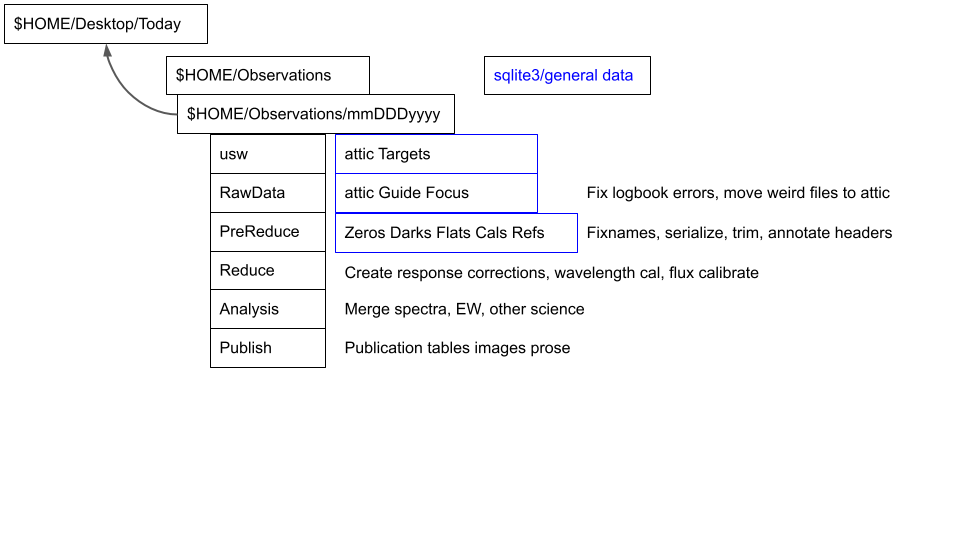
\includegraphics[width=.8\textwidth]{images/Overview1.png}
\caption{Basic Pipeline Steps} %% \caption{{\tiny{citation}}}
\label{figure:basicpipeline}
\end{figure}

\clearpage

\setcounter{section}{0}

\ifx\documentisdraft\drafttest
\linenumbers    %%%%%%%%%%%%% DRAFT
\fi

\clearpage
\pagenumbering{arabic}
%% \fancyfoot[ELF,OLF]{Go to: \hyperref[sec:contents]{Contents}}
%% \fancyfoot[ERF,ORF]{Go to: \hyperref[sec:index]{Index}}
%% \fancyfoot[ECF,OCF]{Page \thepage}

\fancyfoot[LF,OLF]{Go to: \hyperref[sec:contents]{Contents}}
\fancyfoot[RF,ORF]{Go to: \hyperref[sec:index]{Index}}
\fancyfoot[CF,OCF]{Page \thepage}


\section*{Overview}

This document refers to the new IRAF/Pyraf Noirlab 2.18 supported
Pyraf3 : \url{https://iraf.noirlab.edu/} and
\url{https://github.com/iraf-community/pyraf}.

The document covers details system setup for observing and reduction.
We are using a Raspberry Pi/libindi/Ekos for managing cameras and
other details. Once data is captured it is quickly copied to a more
stable platform for backup and reduction. We have IRAF/PyRAF installed
on the RPi to facilitate focus and quick tests of the images.

IRAF/PyRAF is considered a terminal based ``command line
environment'', a very flexible way to use small programs to achieve
large goals. GUI environments restrict users to 'canned' logic. Many
people are uncomfortable with command line work. It requires learning,
practice, and frequent use to maintain a fine edge needed for scientific
data reduction.

This \dhl{Bon Mots} document represents many tricks that one may use
to avoid editing temporary files by hand and to provide an audit trail
for projects.

Go to Section \ref{sec:complexexample} and briefly ponder the code with an
eye towards: ``What is this person thinking!''.

\section{Typography} \label{sec:Typography}

The typographic conventions used in these notes.

Here \llbox{k} means hit the ``k'' on the keyboard. 

\subsection*{Text}

The document uses \dhl{color} to make something \dhl{interesting},
stand out from the text.

\subsection*{Examples}

Examples, in general, state a \dhl{Goal}, the statement of the
\dhl{example}, and \dhl{Prose} to describe the 'thought model' or a
statement about takeaways from the example, and where needed some
exercises. These are presented in this format:

\begin{quote}
\goal Demonstrate a goal. Yes this example was a goal.\\ \example Give
an example of some syntax.\\ \prose Hey, put a linguistic pattern into
your ``thought process'' for that syntax.\\ \exercise[-a] Pick up your
pencil and start your notebook! \\ \exercise[-b] Time to stand for a
minute. \\ \takeaway Tie the thought process to a concrete goal and
example and begin documenting and checking your work.
\end{quote}

\subsection{Margin Annotations}

There are places in the notes where margin annotations are used
to draw attention to something important. In some cases this will
be a note to the author to add/clarify a section of text. Usually
more information may be found in the End Notes section of the document.
\ltodo{Example of Margin Note}{Added a note to demonstrate the note process.}

\subsection{Index}

This document is written in \LaTeX. The \LaTeX environment permits developing
and maintaining a set of bibliographic references, a great index and glossary. 

\section{The Unix and the Data ``Big Picture''}

This document is centered around the Ubuntu 22.04 LTS release using
the NOIRlab IRAF/PyRAF 2.18 pagkage. It offers a paradigm developed
over years of working with IRAF. This leverages Unix. The astronomy
community uses Apple Mac computers that still retain enough about Unix
to allow easy porting of IRAF and friends to that platform, even the
Apple Mx processors.

Win1X requires a VirtualBox (the Microsoft HyperV does not work well
enough).  The client operating system installed in the Virtual box may
be Fedora (the community version of Red Hat Enterprise Linux or RHEL).
This allows installing ESO packages that leverage the RHEL environment.
\textbf{Note}: Some AMD processors will not run hypervisors.
\index(RHEL!ESO) \index{RHEL!Win1X} \index(VirtualBox)

In Unix everything is a 'file'. Programs should be small, perform a
duty and do it well, permit some options. A program takes input from
``standard-in'' (\dhl{stdin}), does its work and puts its output to
``standard-out'' (\dhl{stdout}). Any errrors are reported via
``standard-err'' (\dhl{stderr}). Unix uses a device called a \dhl{pipe}
to send the output from one program into the stdin input of another.
Thus programs can be linked together on one line. 

OK, some programs are huge, and this paradigm does not necessarily
apply. But all the basic Unix utility programs like \dhl{ls}, \dhl{find},
\dhl{grep} etc work this way.

Changing from a GUI paradigm to a command line paradigm is one of the
hardest things for many reading these notes to do.

The Unix philosophy set forth by Ken Thompson, as documented by Doug
McIlroy \cite{McIlroy1978,McIlloryPhilosophy}:

\begin{quote}
Make each program do one thing well. To do a new job, build afresh
rather than complicate old programs by adding new "features". Expect
the output of every program to become the input to another, as yet
unknown, program. -- McIlroy
\end{quote}

GIUs are monolithic in design.\footnote{A GUI is a great way to encapsulate
a process where variation in the process is shuned and discouraged. Scientific
data is noisy and physics is opinionated -- this requires a careful attention
to detail not managable with GUI environments.}

One negotiates with Linux's root process to connect to the Linux
system, where the login process drops the user into a \dhl{shell}. There are
several shells to choose from -- here we will stick with \dhl{bash}
\index{bash}. \textbf{\emph{Note:}} \dhl{/usr/sh} defaults to an abbreviated shell
called \dhl{dash} on most Debian systems. \index{Unix Shell!intro}

\begin{quote}
``On a UNIX system, everything is a file; if something is not a file, it is a process.'' --
Machtelt Garrels, ``Introduction To Linux: A Hands On Guide''
\end{quote}

Peter Freeman \cite{freeman1975software} offered a model of a computer
(and a good operating system) as one of a \dhl{Processor},
\dhl{Memory} and \dhl{Transducer} (PMT) \index{computer!PMT}. The
processors today have less than one core to multiple cores, symmetric
arrays of cores and massively parallel cores.  Even the core of yore
is being supplanted by compute engines, the current popular one is the
GPU with $10^{\$}$ tiny cores.

Files are specialized and fall into classifications like: directories,
special files, links, sockets, named pipes.

There is only one file system and it starts at ``/'' or \dhl{root}.
We tend to think of files as residing on a disk drive. Multiple
drives, and their multiple partitions are simply ``mounted'' at
a location under the ``/''   root directory. Examples are
usually called something like /usr2. Disks on other machines
are usually found, conceptually as a sub-directory the /mnt directory.

\subsection*{The Shell ,``commands'', and Scripts}

The computer sees typed text as groups of characters separated by some
delimiter. Usually the delimiter is a combination of one or more
spaces and/or tab characters. These are called \dhl{whitespace}.

So all of programming takes a stream of complex symbols that, when
taken together, direct the computer to take some safe action. Linux
uses whitespace to set apart each symbol. 

Commands are designed to be typed at the keyboard and are usually
highly abbreviated. One of the handiest commands is \dhl{man}.

\example Use the ``\dhl{man}'' command \\
\prose Hey, what does the man (or ls or ln) command do?\\
\exercise Enter ``\dhl{man man}'' at the shell prompt.\\
\takeaway Read about how man works!\\
\exercise[-b] Enter ``\dhl{man ls}'' at the shell promot.\\
\takeaway Note: it says ``list directory contents'' so the abbreviation
of ``ls'' makes sense. It also offers up a myriad of options.\\
\exercise[-c] Try ``\dhl{ls -l}'' to see details of each file, one per line.\\
\takeaway A way to determine if files are normal files, directories or
links.

One of the oldest Unix commands is ``ls'' used to 'LiSt' directories and
their contents in interesting ways.

\section{Files and Directory Structure}

IRAF/PyRAF 2.18 is installed at a system level, and customized for each user.
The \dhl{mkiraf} command will create a {\textasciitilde}/.iraf directory.

IRAF uses two key files: \dhl{login.cl} and \dhl{loginuser.cl} to select from a myrid
of options and packages one will use for the tasks at hand. The \dhl{login.cl}
file now resides at \dhl{/etc/iraf/login.cl}. The loginuser.cl is located
at {\textasciitilde}/.iraf.loginuser.cl -- this is the file you change.
\textbf{\emph{Note}}: a single line with the word ``keep'' is required at the bottom
of this file.

The loginuser.cl file may be used to add your own special on-off commands,
and to leverage \dhl{foreign} tasks (usually other handy programs on the
path). \index{IRAF!foreign tasks}

Each IRAF task has a set of parameters, managed in the {\textasciitilde}/.iraf/uparam
directory. 

\textbf{BEWARE}: IRAF tasks are ``sticky''. When you change something it remembers the new
thing. The IRAF command \dhl{unlearn <task>} will cause the task to revert to
its defaults. \index{IRAF!sticky}

Other files:

\vspace{-.15cm}
\begin{enumerate}\addtolength{\itemsep}{-0.5\baselineskip}
%\setcounter{enumi}{N}
   \item  {\textasciitilde}/.bashrc, include your own {\textasciitilde}/.iraf-aliases
   \item  login.cl  - traditional configuration, don't edit this one.
   \item  loginuser.cl - configuration to users special taste.
   \item  pyraflogin.py - while not official has handy python functions
   \item  home\$/uparm - where the system keeps parameter files.
\end{enumerate}

\subsection{Directory Layout}

There are two quintessential things about data: 1) preserve the data
and 2) be able to audit processing of the data.

The most important thing is the preservation of the data. Backup,
Backup and Backup again. Then make a copy. It is best to save data on
multiple machines, or to the cloud. Google Drive (and other places)
offer 5TB of data storage for a quite reasonable fee.

All camera data consists of \dhl{16-bit unsigned ADU} values per pixel from
the camera. It is not necessary to change and/or archive raw data with
float values. The QHY600M images are 9600 x 6433 x 2 bytes of image,
roughly 13e6 bytes. Therefore 5TB of disk space will hold roughly
380,000 images. At 3 images per minute for an 8 hour night you get
2400 days of observations for 5TB of disk storage. That's 12 years in
practical terms. However, transferring these images over the net is a
problem.

% (iv (setq tmp (* 9600 6433 2)))    123513600  
% (iv (setq tmp (/ 5e12 13e6 )))    384615
% (iv (setq tmp (/ 384615 (/ 1440 3 3) 200 )))   12     2403

The \dhl{{\textasciitilde}/Desktop} directory allows software acquisiton software to be
configured once. Each night should be copied and archived. 

\begin{quote}
\begin{figure}[h!]
\dirtree{%
.1 {/home/user}.
.2 Observations.
.3 usw  - target lists, cl, notes, other generic things.
.3 ddMMMyyyy  - Date of sunset at Observatory.
.4 usw  - target lists, cl, notes, other generic things.
.4 RawData  - data: warts, blisters and all made read only.
.4 PreReduce  - copy RawData, and work here.
.4 PreAnalysis - pick up analysis for files.
.4 Reduce - Major IRAF/NonIraf reduction.
.4 Analysis - Major IRAF/NonIraf analysis.
.2 Desktop.
.3 Today - where all ``tonights'' observations go.
}
\label{figure:dirlayout}
\end{figure}
\end{quote}


The directory \dhl{usw} is used in lieu of etc. It is the German language
way of saying the samething - \dhl{und so wieder} ``and so again''.
In Unix \dhl{etc} contains loosely related information. For example
puruse \dhl{/etc}, where the system keeps configuration information
of a global level. It is so overloaded something unique is desired.

With this layout, the \dhl{{\textasciitilde}/Observations/usw}
directory contains side files of importance your overall personal
observing strategy. Files, like ds9 region files, special catalog
files general tools etc are stored here. Make subdirectories that
hold common information for different sites or instruments. Copy
those data into a nightly structure as needed.

Data is taken at night. Use dates that reflect the date of sunset
at the site where the data were obtained.

Using the KStars/Ekos/libindi, running on a Raspberry Pi for example,
or a local machine you may want a \dhl{{\textasciitilde}/Desktop/Today} directory
for each night's observing run. In this way the capture/observatory
software does not have to be configured each night. That export directory
remains the same. At the end of the night, simply rename the directory.

Date formats may be confusing, and subject to a computer's LOCALE
subsystem Nobody can make their minds up about date formats.

\centerline{{\huge{{\color{darkred}{SO! SPELL THE DATE OUT!}}}}}

The \dhl{ddMMMyyyy} directory uses the 1 or 2 digit day of month,
followed by the text abbreviation of the month, followed by a 4-digit
year (lets don't play Y2K again). 

This format makes the shell's text completion a quick way to move around.
Text completion involves typing a few starter characters of the file/directory
name then hit the tab. It will advance to the next non-unique thing.

Underneath \dhl{ddMMMyyyy} is the usw directory for tonight's work. The
target list, special catalog file of reference stars etc, the scheduler's
input. Here we store the \dhl{reduce.cl} or \dhl{reduce.py} script
template to be developed for these particular data.

The RawData/PreReduce/PreAnalysis/Reduce/Analysis directories are
cascading stages of data. You may use an \dhl{attic} directory where
to sideline unrelated or terrible images.

You can automate file reduction by using sub-scripts/tasks within the
melange of IRAF/PyRAF/bash/python/whatever language programs and then
leveraging Python and cl into making a
\dhl{OBSERVATION/usw/reduce.pyraf}\index{reduce.cl}
script\index{reduce.pyraf} script for the data. Save this as a template in
the general \dhl{usw} directory, and copy in to each observation's repository.
Detailed example is in Appendix \ref{sec:ReducePyrafControlFile}.

At this time PyRAF (a mix of ecl and Python) does not act well as a
``script'' due to the hack that adds ecl syntax to the GNU runline command
input. It uses the raw input directly and side-steps \dhl{stdin}. This
violates the Unix philosophy of each program should take its input from
stdin, process its results and put the results into stdout.  This
allows one to pipe programs together to achieve an ultimate goal.

Scripts may be written in the \dhl{.cl} language (really ecl or extended cl),
actual PyRAF (\dhl{.pyraf}), or hacked into PyRAF with the \llbox{!}
cl prefix as you go along.

\textbf{\emph{Note}}: The \dhl{.pyraf} scripts blend python and PyRAF together.
See the complicated example of how to deal with APO NICFPS camera
images.

\section{Critical First Steps}

It is critical you properly install the IRAF/PyRAF3 packages. This
release looks for a {\textasciitilde}/.iraf directory that may not be fully integrated
into the rest of IRAF.

You may make a soft link of \dhl{\home/iraf} to \dhl{\home/.iraf}:

\dhl{ln -s \home/iraf \home/.iraf}

The document will continue to refer to \dhl{\home/iraf} as the base
of the IRAF package. 

It is important to use a \dhl{~/iraf/loginuser.cl} file with task
aliases foreign and tasks.\index{tasks!aliases} \index{tasks!foreign
  tasks}

One way to make things simple is to create a bash alias for pyraf that:
\vspace{-.15cm}
\begin{enumerate}\addtolength{\itemsep}{-0.5\baselineskip}
%\setcounter{enumi}{N}
   \item   uses xdotool to change the color of the window's background
   \item   update the PATH and PYTHONPATH to access all the special files you use
   \item   run the system pyraf (note the /usr/bin path is prefix is necessary) 
 with the ``-s'' switch for ``silent'' start.
\end{enumerate}


\begingroup \fontsize{10pt}{10pt}
\selectfont
%%\begin{Verbatim} [commandchars=\\\{\}]
\begin{verbatim} 
alias pyraf="xdotool key shift+F10 r 1;\\
  export PATH="/usr/local/bin:$PATH"; export PATH="/usr/local/astrometry/bin:$PATH";\\
  export PYTHONPATH=$HOME/.iraf; export PATH="$HOME/.iraf/smtsci/bin:$PATH";\\
  /usr/bin/pyraf -s;"
\end{verbatim}
\endgroup
%% \end{Verbatim}

\subsection{IRAF/PyRAF Tasks and Packages}

IRAF, from ye-olden times, uses \dhl{packages} containing help text
and parameter files to hold values from run-to-run together with the tasks'
executable code.
\index{IRAF!tasks} Tasks are ``programs'', usually written in FORTRAN
or in cl proceedural code. Some are written in C/C++.

\dhl{BEWARE}: IRAF is \dhl{sticky}! It retains parameter values from
run-to-run that can perpetuate errors. Review all the parameters to be
sure your reductions are proper. These values are stored in the
\dhl{~/iraf/uparm} directory.

Tasks are built into IRAF/PyRAF but are only loaded once. Each time
they are used -- they are in memory and already part of the CPU thread
you are using. Thus they very fast. Using \llbox{!} shell-escape or a
\dhl{\$foreign} task causes Unix to create a new heavy-thread with
significant overhead (especially in a loop).

IRAF has a habit of loading images into memory and keeping them there.
Some tasks will modify the in-memory image but not write it back to
the disk. Work may be lost. See Section \ref{sec:FITSFiles} for quick
details.

IRAF has a neurotic habit of \dhl{sometimes} adding an extent to
certain FITS files! This is the case with master darks and flats
and a handful of other operations.

It is best to develop your \dhl{reduce.pyraf} script in an editor, one line
and step at a time, then cut/paste edited lines at the interactive
prompt. When you make a mistake -- and you will -- you can start over
with a fresh copy of data and stop short of the mistake. Pick up and
go again.

\subsection{Full On Python Hacks}

\example Python's \dhl{import iraf} statement allows for operations like: \\
\prose I want to use IRAF's imstat command to get a binary value, assign
the value to my python variable. \\
\exercise Enter: \\
{\color{verbcolor}{
\begingroup \fontsize{10pt}{10pt}
\selectfont
%%\begin{Verbatim} [commandchars=\\\{\}]
\begin{verbatim} 
mymean = float( iraf.imstat(images='*fits',fields='mean',format=iraf.no,Stdout=1)[0])
\end{verbatim}
\endgroup
%% \end{Verbatim}
}}

\takeaway The task has a pythonic wrapper, contained in the iraf.py
module's namespace.  It needs a list of files, we only want the one
field \dhl{mean}, we do not want the headers (format=iraf.no). The
phrase Stdout=1 (note capitalization) returns the text as a string
rather than printing on the terminal. But! The string is actually an
array, so we want the first bit. But! that bit is a string, and we
need to convert to binary with the \dhl{float} python function.

where \dhl{mymean} is now a proper python float. Yes, convoluted, but
its buried in a scrip and available for your use. \index{Stdout}

\subsection{Task Parameters}

Always be aware of the:
\vspace{-.15cm}
\begin{enumerate}\addtolength{\itemsep}{-0.5\baselineskip}
%\setcounter{enumi}{N}
   \item    ~/iraf/uparm directory
   \item    lparm <taskname> command to list parameters.
   \item    \dhl{unlearn <task>} command.
   \item   help <task> and look at the see also part at the bottom.
\end{enumerate}

\section{Goals}

The main goal of scripting is not the script, it is the result. Good
data results do not come from good scripting -- but come from good
planning, good execution of the plan and attention to configuring
your tools.


\subsection{Things to remember}

IRAF \dhl{cl} morphed into PyRAF \cite{2006hstc.conf..437G} to allow a more
powerful \dhl{cl} by hacking the Python \dhl{readline} subsystem. The
grammar of python was altered to allow for a ``direct entry'' of most older
\dhl{cl} commands. Direct access to the underlying tasks was
accomplished with a ``cythonic'' interface into underlying code. An ``iraf''
module was added to support programming calls to IRAF tasks and using 
a special Python \dhl{keyword} argument Stdout to return output as a string.
Parsing this string with python allows chaining \dhl{cl} commands together
for a goal.

A tremendous amount of power is available for you to mix and match to meet
your specific needs. 

\subsection{Observation Directory}

One can not expect proper structure by simply importing a night's
observations, warts blisters and all. Files will be scattered all
over, mis-named, bad headers, useless(!), and other oddities. But copy
the data into date/RawData. See directory layout table \ref{figure:dirlayout}

Open date/usw/reduce.cl in your favorite editor. Anything you want
to type into PyRAF -- type it into the reduce.cl file. Then cut/paste
the command to PyRAF. This means when you make the mistake -- you
can remove the last line, save the reduce.cl file, and rebuild
to that point. Yes, some interactive things will or may happen.
Try not to make too many mistakes.

\vspace{-.15cm}
\begin{enumerate}\addtolength{\itemsep}{-0.5\baselineskip}
   \item   cd ~/Observations
   \item   mkdir 22Feb2022 \# date of sunset at the observatory
   \item   cd 22Feb2022
   \item   mkdir -p Plan RawData PreAnalysis Analysis Publish usw
   \item   mkdir -p PreAnalysis/{Bias,Darks/{s300,s3},Flats,Comps} \# prior knowledge
   \item   cd RawData
   \item   cp -pr /mnt/NAS/22Feb2022/* .  \# copy the raw data
\end{enumerate}

Now the plan for observations and initial PreAnalysis results is in 
place. The \dhl{usw/reduce.cl} script is the key. 

Good observations are the result of good planning. Make the list of targets,
determine offsets and guide stars, create a ds9 region file in ICRF WCS
coordinates for the field of view and possible orientations of the instrument.
If possible download the preparation package from the observatory and take
time to prepare. \index{planning}

\begin{figure}[h!]
\centering
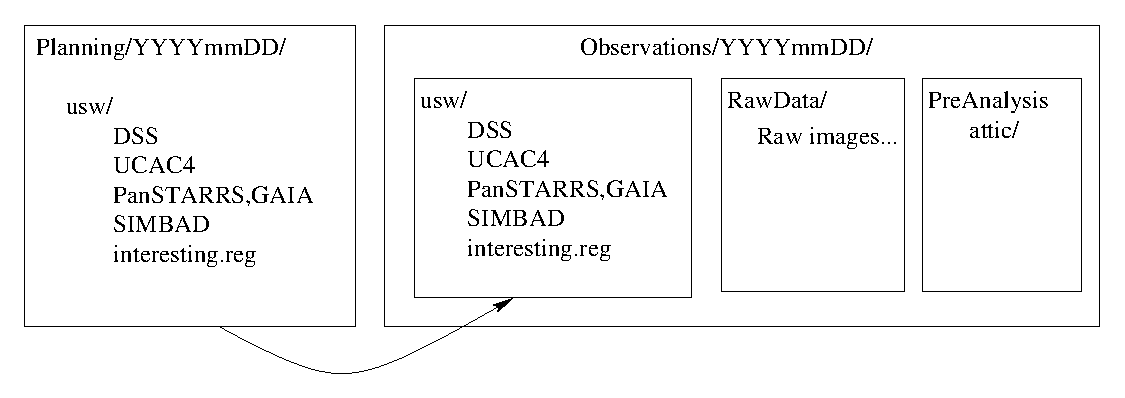
\includegraphics[width=.4\textwidth]{images/Overview.eps}
\caption{The observations directory was in place with the plan.
Load up the raw images. Then copy raw data to pre-analysis.} %% \caption{{\tiny{citation}}}
\label{figure:GoalsOverview}
\end{figure}

\clearpage
\subsection{The main tricks}

Note: Unix files do not rely on their extensions. A Unix extension is a social
convention. Many authors use two files, like \dhl{in.txt} and \dhl{out.txt}.
They will use an editor to change the bits of one to another. 

I recommend using goofy file names, like \dhl{xxx} and \dhl{l.l}, when seen
they may be removed. The filename \dhl{l.l} is real easy to type because
the \llbox{l} and \llbox{.} are right next to each other!

The \llbox{/}\llbox{/} sequence is the cl concatenation operator, used to
join two strings without intervening whitespace.

Instead of having the input files in in.txt, then editing to make unique
output names -- simply prepend a string, with some meaningful context
to the @file. 

The order of operations may be to
\vspace{-.15cm}
\begin{enumerate}\addtolength{\itemsep}{-0.5\baselineskip}
%\setcounter{enumi}{N}
   \item   t\_ trim a file.
   \item   c\_ cosmic ray removal
   \item   z\_ to zero correct
   \item   d\_ to dark correct
   \item   f\_ to flat a file
\end{enumerate}


etc. data.fits, after processing may be \dhl{f\_d\_z\_c\_t\_data.fits}.

So PyRAF has several tricks up its sleave:
\begin{itemize}
\addtolength{\itemsep}{-0.5\baselineskip}
   \item   It can act like a basic ``calculator'' just by typing standard python at the
PyRAF command prompt. Remember to ``import'' packages like math and numpy.
   \item It works with list of files. These are refered to as ``list''
     or ``at'' files. They are like {\color{verbcolor}{\verb#@l.l#}}
     where the file ``l.l'' has a list of filenames -- one per line.
   \item You can take the files in ``l.l'' and produce new files with
     the same name but prepend a clause to the
     filename!\\ \textbf{E.g.:}
     {\color{verbcolor}{\verb#imarith @l.l - zmaster.fits z_//@l.l#}}\\ will
     subtract the zero master from each file in ``l.l'' and make a
     corresponding {\color{verbcolor}{\verb#z_filename.fits#}}.
\item PyRAF is a a replacement for {\color{verbcolor}{\verb#cl#}} (actually
ecl). You can loop {\color{verbcolor}{\verb#.cl#}} commands together
with bash commands into the mix to do work using:\\
{\color{verbcolor}{\verb#cl < ~/iraf/fit2fits.cl#}} to bring a Vendor's
fit format to the PyRAF standards.
\end{itemize}

It has a few oddities, inherited from the ecl lashup of the Pythonic 'readline' hack,
ripped from a \dhl{reduce.cl} script:

\vspace{-.15cm}
\begin{enumerate}\addtolength{\itemsep}{-0.5\baselineskip}
   \item Oops! Its Python 2.7 so write helpers like \dhl{trim} and
     \dhl{fitsls} accordingly.
   \item   Most of the IRAF \dhl{cl} commands work
   \item   \dhl{set OBSROOT=/home/me/Observations/23Feb2022}
   \item   \dhl{set OBS=OBSROOT\$/PreAnalysis}
\end{enumerate}

The IRAF command \dhl{chdir} \index{cl!chdir} changes directory while respecting
the IRAF use of iraf-environment variables.

You can escape to bash by starting the line with a bang (!). This
allows developing handy bash scripts to store in iraf/bin.

\clearpage

\subsection{System Setup}

I presume the use of the Ubuntu 22.04 Linux distribution from Canonical\texttrademark.

%% Under Microsoft Windows\texttrademark Pro, there is a system called \dhl{Hyper-V}.
%% It is very ``light-weight'' virtualization layer for Windows that permits
%% the seamless of an essentially containerized Ubuntu 22.04 + anaconda and other
%% Linux based tools while maintaining contact with the Windows file system,
%% the network etc. \index{Windows!Hyper-V}.

%%Under Linux you are running Linux anyway.
MacOS is very Linux like, even on their M1 processor series.

Install the Anaconda package without the Navigator. This brings in
a massive amount of power, including Astropy \cite{astropy:2013} \cite{astropy:2018}
\cite{astropy:2022}.
\vspace{-.15cm}
\begin{enumerate}\addtolength{\itemsep}{-0.5\baselineskip}
   \item    Necessary:
\vspace{-.15cm}
\begin{enumerate}\addtolength{\itemsep}{-0.5\baselineskip}
   \item    Ubuntu 22.04/Mac OS + many apt-get packages
   \item    Anaconda (Python 3+)
   \item    Astroconda PyRAF recipe (a python2.7 env)
   \item    Ubuntu aptitude iraf/pyraf packages
   \item    Sextractor
   \item    Current SAOImage/ds9
   \item    Current Astrometry.net + 4200 and GIAI data
   \item    Fitsverify \cite{fitsverify-1}
   \item    GitHUB sasiraf package (currently private contact author.)
\end{enumerate}
   \item    Optional
\end{enumerate}

\subsection{Unix\texttrademark Aliases}
A few aliases need to be setup.

\ltodo{Add Aliases}{Update/add aliases for bashrc file.}

\begin{figure}
{\color{darkred}
\begingroup \fontsize{10pt}{10pt}
\selectfont
%%\begin{Verbatim} [commandchars=\\\{\}]
\begin{verbatim} 
function pyraf  { #export PYTHONPATH=$HOME/iraf;
                  export PATH="/home/wayne/anaconda3.8/envs/geminiconda \\
                     /bin:$HOME/iraf/smtsci/bin:$PATH"; (folded line)
                  source activate geminiconda;
                  xdotool key shift+F10 r 6;     # change terminal color
                  $HOME/anaconda3/envs/geminiconda/bin/pyraf -s $*;
                }
\end{verbatim}
\endgroup
%% \end{Verbatim}
}
\caption{An entry into the aliases file, using the Gemini pyraf installation.}
\label{fig:geminialias}
\end{figure}

This is a little-bit complicated:
\vspace{-.15cm}
\begin{enumerate}\addtolength{\itemsep}{-0.5\baselineskip}
   \item   The PYTHONPATH allows pyraflogin3 to be imported after start.
   \item   This assumes \dhl{~/iraf/pyraflogin.py} is present.
   \item   The function in figure \ref{fig:geminialias} tells Anaconda to activate
     the geminiconda environment
   \item   The xdotool allows the color of the terminal window to be changed.
   \item   PyRAF is then started, the \dhl{-s} switch is quiet about packages loaded.
   \item When pyraf starts, it loads \dhl{login.cl} which in turn
     loads my \dhl{loginuser.cl} scripts.
\end{enumerate}

\subsection{Initialization files}

PyRAF uses \dhl{~/.iraf/login.cl} to manage system level commands and should
not be edited -- except to ensure that \dhl{cl < "home\$/iraf/loginuser.cl"} is
enabled. Edit the \dhl{loginuser.cl} file and pile changes.
 \index{Initialization!login.cl}
\index{Initialization!loginuser.cl}

A special \dhl{~/iraf/pyraflogin.py} file can 'extend' the Python
environment.  A sample file is available with this package. It
requires the special alias to start PyRAF. It adds simple
\dhl{matplotlib} plotting and some handy fixer-upper functions. See
that package for documentation. \index{Initialization!pyraflogin.py}

\subsection{Initial Steps}

This process uses a user-defined  directory structure as shown in
figure \ref{figure:basicpipeline}. 

The main steps are:
\vspace{-.15cm}
\begin{enumerate}\addtolength{\itemsep}{-0.5\baselineskip}
   \item   Layout basic directory structure:


   \item  Add a few toplevel soft-links for non-sentient file browsers.
\dirtree{%
.1 \$HOME/.aaatoday linked to \$HOME/Desktop/Today.
.1 \$HOME/.aaareduce linked to current working reduction.
}

   \item   Planning - load up the \dhl{\$HOME/Desktop/Today/usw} directory with
FOV files, and anything related to observatory etc.

   \item   Observe
   \item   Move dhl{\$HOME/Desktop/Today} to dhl{\$HOME/Desktop/Observations/mmDDDyyy}
date of sunset at the observatory of the instrument.
   \item   Make a safe backup.
   \item   Start the process of reducing the data.
\end{enumerate}

The script provides the audit trail you used. Modify this for each
instrument setup, and for each filter type etc.  Essentially the same
for spectroscopy -- just watch the statistics sections.

You may not need darks, and the flats will be different.

When, not if, you mess up you can delete the PreAnalysis directory, fix
the above script, and start over. As you move deeper into the file
processing, the script becomes more valuable.


\clearpage
\subsection{PyRAF Calculator Mode}

\goal Demonstrate borrow Pyraf as a calculator within PyRAF. Determine
the mean plus 3 times the standard deviation for a limit.

\example 
{\color{verbcolor}{\verb#imstat zmaster.fits fields=mean,stddev#}} \\
you find the mean is 346 and the stddev is 47.

\exercise How many pixels in the zero master are 3 or 5 $\sigma$ above
the mean?

{\color{verbcolor}
\begingroup \fontsize{10pt}{10pt}
\selectfont
%%\begin{Verbatim} [commandchars=\\\{\}]
\begin{verbatim}
from astropy import fits  # DO THE IMPORTS ONCE
import numpy

f = fits.open('zmaster.fits')    # open the fits file as a cfitsio like
d = f[0].data   # get the data   # structure and just grab the data.
# using some python magic!
(mean,stddev) = map(float,
                   iraf.imstatistics(Stdout=1,fields='mean,stddev',
                      images='zmaster.fits',format=iraf.no)[0].split())
len(d[d> mean + 3.0*(stddev)]) # 25729 pixels matched this example
len(d[d> mean + 5.0*(stddev)]) #  1220 pixels matched this example
f.close()
\end{verbatim}
\endgroup
%% \end{Verbatim}
}


\prose Hey, we're PyRAF, a pythonic interpreter -- so lets really use
Python.  The imports are used to get the modules/functions we
need. The fits.open gets the FITS file open for business; we grab just
the image data as a numpy array of shape
{\color{verbcolor}{\verb#NAXIS2,NAXIS1#}} (switched(!), numbered from
zero now and the data will have overscans if present!) using
{\color{verbcolor}{\verb#d = f[0].data#}}. The
{\color{verbcolor}{\verb#iraf#}} is imported by virtue of we're PyRAF;
the {\color{verbcolor}{\verb#imstat#}} is run as a python function
using {\color{verbcolor}{\verb#iraf.statistics()#}}.  The
{\color{verbcolor}{\verb#Stdout=1#}} tells the task to return the
output not send it to the terminal. The
{\color{verbcolor}{\verb#format=no#}} tells the function to omit the
usual header text etc, and just return the two values requested with
the {\color{verbcolor}{\verb#fields="mean,stddev"#}}.  The output is
one string with two ASCII numbers. These are split into an array, then
the {\color{verbcolor}{\verb#float#}} function converts the strings
into actual numbers -- returned as the tuple
{\color{verbcolor}{\verb#(mean,stddev)#}}.

\subsection{Using Numpy Arrays}
%HEREHEREHERE

Numpy arrays follow the ``C'' indexing scheme, which is ``ordinal'' in nature
(starting with zero). For an (X,Y,Z) index -- the array is referenced \dhl{backwards}:
myarray[Z][Y][X]. This differs from the FORTRAN convention for arrays, ``cardinal''
in nature (counting from 1).

FITS images are stored in FORTRAN order, and in Big Endian format. This makes
difficult for Intel architectures.

This is critical. Data are written into FITS images in so-called \dhl{Big-Endian}
fashion. In Jonathan's ``Gulliver's Travels'', a fictional character encounters
a culture in heated conflict over weather or not one should crack open an
egg on the little end or the big end. Computer aritectures are conflicted on
how to store a larger value, say an integer that spans more than one byte
into a linear address space. Decisions (bad perhaps) were made to store
a 16-bit integer with the byte containing least significant digit first.
The word oxBO is stored with the 0 first then the 0x0B. This was to make
a very early machine fast at ++value operations! We're stuck with that decision
since.

The real issue boils down to the Bad Thing\texttrademark practice of
``type punning'' whereby a block of data in ``Endianess Be Damed''
format is read into memory, then attempts to access it as though it
had the right byte order results in catastropy when data is exchanged
between the types of architectures.

Intel processors are ``Little Endian'' where processors like the Motorla
68000 were ``Big Endian''. 

Data are stored as arrays, with astropy.fits.io open command setting the
data[0] extent as a pythonic numpy array. So the indices are a bit backwards
The fits header would read something like:

\begingroup \fontsize{10pt}{10pt}
\selectfont
%%\begin{Verbatim} [commandchars=\\\{\}]
\begin{verbatim} 
NAXIS  = 2
NAXIS1 = 2048
NAXIS2 = 512
\end{verbatim}
\endgroup
%% \end{Verbatim}

To store a 2D image array. This is ment to denote an image that is 2048 wide and 512
tall. 

\ltodo{numpy vs FORTRAN}{Get into index details.}


The next bits use numpy arrays. Here we use the conditonal indexing
mode common to numpy arrays to get all the pixels that match
expression of the value > the
{\color{verbcolor}{\verb#mean + n times stddev#}}.

Need a ``Quick Calculation'' to find the center of an image to
use as a ``statistics section'' for normalizing?:

{\color{verbcolor}
\begingroup \fontsize{10pt}{10pt}
\selectfont
%%\begin{Verbatim} [commandchars=\\\{\}]
\begin{verbatim}
imhead zmaster.fits   # result is 'zmaster.fits[1368,1364][real]:'
# half size? pick up the [NAXIS1,NAXIS2] from abbreviated imhead result...
(1368//2, 1364//2)   # returns tuple (684, 682)  the '//' is integer divide.
print "[%d:%d,%d:%d]" % (1368//2 - 50, 1368//2 + 50, 1364//2 - 50, 1364//2 + 50)
# [634:734,632:732]  Et Viola! A handy center stat section for normalizing!
\end{verbatim}
\endgroup
%% \end{Verbatim}
}

Make your own functions! Then imexamine -- the comp star and the target star.

{\color{verbcolor}
\begingroup \fontsize{10pt}{10pt}
\selectfont
%%\begin{Verbatim} [commandchars=\\\{\}]
\begin{verbatim}
import math    # DO THIS ONCE
def mag(compmag,compflux,observedflux):
   return -2.5(math.log10(observedflux / compflux) + compmag
\end{verbatim}
\endgroup
%% \end{Verbatim}
}

\exercise Correct for background.

\section{Getting Started}

Configure the system. Copy the login.cl to ~/.iraf. Copy loginuser.cl script
to ~/iraf. \textbf{\emph{Note}} One has a hidden-file dot.

Add the .iraf.aliases file to \dhl{\$HOME} directory and if you like, add it to
the \dhl{\$HOME/.bashrc} file.

Start PyRAF in one window and start Editor in another window. I
recommend emacs or Sublime Text as editors -- they are GUI
oriented. Remember all things have a learning curve.

Why we use the vi editor. Vi is the ``\dhl{Vi}sual Editor'' that sits
on top of a powerful albeit basic Unix editor ``\dhl{ed}. The \dhl{ed}
editor is the basis for the \dhl{sed} the Unix stream editor. Regular
expressions (think wildcards) are very sophisticated and turn up all
over the Linux/Unix system. They are worth the effort to learn. The
``re'' of the grep program (\dhl{g}lobal \dhl{re}gular expression
\dhl{p}rint) program obviously makes heavy use of regular expressions.

The very basic Linux commands are:

\begin{table}[h!]
\centering
\begin{tabular}{| l | l |}
\hline
Command  & Basic Action   \\
\hline
cd    & change directory    \\ 
ls    & list files     \\ 
pwd   & print the current working directory    \\ 
cat   & \dhl{concatenate} file(s)    \\ 
less  & view content of a file    \\ 
man   & the Manual -- print details of a command \\ 
which & show where on PATH an executable is \\ 
rm    & remove files and directories. \\
%% ones-based: \cline{a-b}
\hline
%%\DeleteShortVerb{|}
\end{tabular}
%%\end{minipage}    %% for footnotes  r@{.}l 
\caption{Very Basic Unix Commands}
\label{table:VeryBasicUnixCommands}
%%} % end small etc
\end{table}


\subsection{Very Basic PyRAF commands}

\begin{table}[h!]
\centering
\begin{tabular}{| l | l |}
\hline
Command  & Use   \\
\hline
cl            & run the cl editor                            \\
epar          & edit parameters/launch task                  \\
hedit         & fast/dirty header editor                     \\ 
imhead        & list the header values for a file            \\ 
hselect       & select values from headers                   \\ 
imexamine     & all manor of ways to view images             \\ 
apall         & reduce a spectrum image                      \\ 
identify      & identify spectral lines assign wavelenghts   \\
dispcor       & apply identify results to science spectrum   \\
splot         & view/analyze reduced spectrum                \\ 
imstat        & print mean,min,max,std etc for set of images \\ 
%% ones-based: \cline{a-b}
\hline
%%\DeleteShortVerb{|}
\end{tabular}
%%\end{minipage}    %% for footnotes  r@{.}l 
\caption{Very Basic IRAF/PyRAF commands}
\label{table:VeryBasicIRAF/PyRAFcommands}
%%} % end small etc
\end{table}


\section{Working on subsets of files.}

IRAF uses ``list files'' denoted \dhl{@list.txt}. The \llbox{@} key
as the first character of the filename tells IRAF to open that
file and take from it filenames -- one filename per line. This is
real handy.

Some documents have you make lists, then use an editor to change the
list as you go. They recommend filenames like mylist.txt. This is
cumbersome to type. Try using a simple name like \dhl{l.l}. Note the
\llbox{l} key is very near the \llbox{.} key! Handy to type.  If you
see the file \dhl{l.l} you know you can simply remove it.  The \llbox{!}
as the first character on a command line sends the rest of the line
to the local bash script. This escape mechanism allows you to use
all the power of Unix inside cl scripts.

The command \dhl{!ls -1 *Dar* > l.l} takes all filenames with Dar
in it and lists them out in lexicographical (sorted) order. Here
are some example of ways to build list-files.

{\color{verbcolor}
\begingroup \fontsize{10pt}{10pt}
\selectfont
%%\begin{Verbatim} [commandchars=\\\{\}]
\begin{verbatim}
!ls -1 *fits > l.l
cl < ~/iraf/crall.cl
# all the files are now c_<filename>

hselect c_*fits $I "IMAGETYP ?= 'Bias'"  > l.l
hedit @l.l IMAGETYP zero add+ show- ver- update+
!if test -e zmaster.fits; then rm zmaster.fits; fi  # bash to rm file if exists
imcombine @l.l zmaster.fits combine=median

hselect c_*fits $I IMAGETYP ?= 'Light'"  > l.l
hedit @l.l IMAGETYP object add+ show- ver- update+
imarith @l.l - zmaster.fits z_//@l.l
imarith z_//@l.l - dmaster.fits d_z_//@l.l
imarith d_z_//@l.l / flatmaster_SII.fits f_d_z_//@l.l

# files are now {\color{verbcolor}{\verb#f_d_z_c_filename.fits#}}
\end{verbatim}
\endgroup
%% \end{Verbatim}
}
This makes use of the fact that we can pile on prefixes to
processed files:

\begin{itemize}
\addtolength{\itemsep}{-0.5\baselineskip}
   \item   t - trimmed
   \item   c - cosmic ray reduced
   \item   z - zero subtracted
   \item   d - dark corrected
   \item   f - flat normalized
\end{itemize}

At the end, a flat-normalized file called {\color{verbcolor}{\verb#science.fits#}} will
have the name {\color{verbcolor}{\verb#f_d_z_c_t_science.fits#}}.

Lots of intermediate files lying around: Clean them up!

{\color{verbcolor}
\begingroup \fontsize{10pt}{10pt}
\selectfont
%%\begin{Verbatim} [commandchars=\\\{\}]
\begin{verbatim}
print "Remove residual files."
! (export LC_ALL=C; rm [a-z]_*fits 2> /dev/null;)
\end{verbatim}
\endgroup
%% \end{Verbatim}
}

\textbf{\emph{Prose:}} \textbf{\emph{Hey}} PyRAF send the line to bash; but! using a sub-shell
set {\color{verbcolor}{\verb#export#}} the {\color{verbcolor}{\verb#LC_ALL=C;#}}
shell variable to let bash actually use case sensitive wildcards. Then
{\color{verbcolor}{\verb#rm [a-z]_*fits 2> /dev/null;#}} remove the
file -- and in case there is some whining about the process, send the
whines to the bit-bucket ({\color{verbcolor}{\verb#/dev/null#}}).


\section{Observing}
PyRAF \index{PyRAF!Observing} is a useful tool for spectroscopy. Using
the imexamine command and the 'j' key: set the rplot to wider than a bright
line width. 

% HEREHEREHERE

\clearpage
\section{Overall Philosophical Approach}

This document covers a philosophy --- a set of general tools and
scripts to take and reduce data.

In this case some location like {\color{verbcolor}{\verb#/opt/myobs/iraf/#}}
or {\color{verbcolor}{\verb#~/iraf/#}} contains a number of small generic
{\color{verbcolor}{\verb#.cl#}} scripts to handle specific needs. These
are specific to certain conditions -- like a package that writes {\color{verbcolor}{\verb#.fts#}}
instead of {\color{verbcolor}{\verb#.fits#}} files. Routines to remove pesky
spaces that GUI users like to use; get rid of multiple ``dots''; plus signs
etc. 

\vspace{-.15cm}
\begin{enumerate}\addtolength{\itemsep}{-0.5\baselineskip}
   \item   Create a planning directory. Rename to Observations/directory
when the plan is executed.
   \item   Create a ``usw'' directory to hold the plan, collect pre-analysis information:
\vspace{-.15cm}
\begin{enumerate}\addtolength{\itemsep}{-0.5\baselineskip}
   \item   DSS image -- ds9 Analysis \menu Image Servers
   \item   Region files, catalog files for ds9 -- ds9 Region \menu Shape ...
   \item   Photometry reference stars --- ds9 Analysis \menu Catalogs \menu Database \menu UCAC4;
or with the Aladin application and TOPCAT make one the hard way. (PanSTARRS DR1).
   \item   Bibliographic information -- Browser and SIMBAD for the target(s).
   \item   Gather any existing bad pixel masks -- previous runs; observatory supplied files.
\end{enumerate}

   \item  Gather raw data --- stay up all night
   \item  Archive raw data as a RawData and make read only --- back to your {\color{verbcolor}{\verb#Observations#}} directory:\\
{\color{verbcolor}{\verb#(cd Observations/YYYYmmDD; mkdir -p RawData; cd RawData; rsync <from somewhere> .; chmod -w -R *#}}).
\end{enumerate}


\vspace{-.15cm}
\begin{enumerate}[resume]\addtolength{\itemsep}{-0.5\baselineskip}
   \item   Copy raw data to a PreAnalysis directory -- do not damage any
raw data whatsoever. Make the PreAnalysis files writable:\\
({\color{verbcolor}{\verb#cd Observations/YYYYmmDD; mkdir -p PreAnalysis; cd PreAnalysis; cp -pr ../RawData/* .; chmod +w -R .#}})\\
Clean data and make initial analysis files:
\vspace{-.15cm}
\begin{enumerate}\addtolength{\itemsep}{-0.5\baselineskip}
   \item   Fix the filenames --- {\color{verbcolor}{\verb#cl < ~sbo/iraf/fix_sbig.cl#}}
   \item   Fix the headers--- {\color{verbcolor}{\verb#cl < ~sbo/iraf/fix_headers.cl#}}
   \item   Trim (remember) overscan --- see above
   \item   Remove bad WCS especially from zero/dark/flats {\color{verbcolor}{\verb#cl < ~sbo/iraf/fix_sbig_wcs.cl#}}
   \item   Remove cosmic rays ---  {\color{verbcolor}{\verb#!ls -1 *fits > l.l#}}
followed by {\color{verbcolor}{\verb#cl < ~sbo/iraf/crall.cl#}}
\item Other basic reduction steps to be covered elsewhere:
\begin{enumerate}\addtolength{\itemsep}{-0.5\baselineskip}
   \item   Make any bad pixel masks 
   \item   Make master zeros and darks 
   \item   Make master flats 
   \item   apply zeros,darks,flats to science images
   \item   add new WCS or de-distort and add new WCS
   \item   extract photometry
   \item   combine images for deeper photometry
   \item   freeze this work
\end{enumerate}
\end{enumerate}


   \item  Copy the PreAnalysis data into an Analysis Directory.
(Any damage here is quickly recovered from PreAnalysis.)\\
{\color{verbcolor}{\verb#!(cd ..; mkdir -p Analysis; cd Analysis; cp -pr ../PreAnalysis/f_d_z_c_t* .)#}}
\end{enumerate}


A break down of the above steps reveals the need to make/use
certain scripts (some shown in red in context above):

\vspace{-.15cm}
\begin{enumerate}[resume]\addtolength{\itemsep}{-0.5\baselineskip}
   \item   Fix the filenames: remove dots, spaces, dashes other special characters.
   \item   Fix the headers: Observatory/Vendor non-IRAF keywords to IRAF
keywords; Very-Non-Standard keywords like PCOUNT and GCOUNT
   \item   Pinpoint is good enough for tracking (still takes a while to apply
and will fail) but is not accurate.
   \item   Single Pixel errors from cheap cameras, inevitable cosmic rays need
to be mitigated in raw zero, dark and flat frames.
   \item   Masks provide locations in pixel coordinates of defects that can ruin
the science.
   \item   Adding a new WCS will help to quickly align images. This may be enough
if there is no distortion, de-distort with flux conservation where possible.
\end{enumerate}


You can stop here and defer photometry to the analysis step. However,
you can extract photometry using sextractor and a few tricks.

Combining images is an art.


\textbf{\emph{Main goal:}} to develop a \textbf{\emph{compact}} set of
skills with Unix/Python/PyRAF/IRAF to create a
\textbf{\emph{collection}} of IRAF scripts to process images from two
cameras, three telescopes using vendor's software. In this sense,
``compact'' means: the basic IRAF commands; python, bash and Unix
tricks and commands; a basic use of SAOImage/ds9. A familiarity with
command line operations and vocabulary to support planning, executing,
reducing data and publishing photometic data. Summary: the course is
designed to introduce astrophysical hands-on research -- not the
tedious nature of the related software tools.

Examples, long and short, will provide an overview of all the weird/odd ways
Bash/IRAF/PyRAF and Python are used is in Appendix \ref{app:PutItTogether}.

\textbf{\emph{The Problem:}} PyRAF is a ``pythonic''
wrapper/controller of collection of IRAF tasks/commands that in turn
are based on the Unix operating system. The long path to getting a
handle on PyRAF is to build on knowledge gained over time: starting
with Python, then Unix in general and the bash shell in particular,
then IRAF commands and tasks. This is hard to do in two weeks.

\textbf{\emph{Exercise:}} we'll jump into the middle of the mess and
build as we go. To temper this exercise, examples are from a third
observatory and vendor's software -- this is to
\textbf{\emph{prevent}} a simple cut/paste without taking the time to
understand each fragment of the provided example code.


\section{PyRAF, IRAF and Unix (bash)}

IRAF was developed in a slow rather ad hoc fashion, its birthday
established by Donald Wells \cite{FITSBirthday} as 28 March 1979,
real development started in 1981 and was it put to use in 1984
\cite{1993ASPC...52..173T}.  At the time researchers at various
institutions using various computing platforms developed ``packages''
that were brought together at NOAO under IRAF (Image Reduction and
Analysis Facility). It was developed under Digital Equipment
Corporation's PDP and Vax computing environments as well as Unix. The
result today reflects coding and use patterns in vogue since that
time. \index{IRAF!history}

The original IRAF used code from a book that ran afoul of copyright
infringements. While still suited for academic work, the work
was dropped by AURA and taken up by a Github based community. There
were several issues with the older 2.14 code. FORTRAN's COMMON and
EQUIVALENCE blocks did not translate well from 32 bit architectures
to 64 bit architectures. The copyright and FORTRAN issues were resolved,
and released as version 2.17.

\clearpage
From \cite{NOIRLabReleaseNote} page:

\begin{quote}
The Image Reduction and Analysis Facility (IRAF) is a general-purpose
software system for the reduction and analysis of scientific data. Its
development started in 1984 at the National Optical Astronomy
Observatories (NOAO) in Tucson, Arizona. As of January 2024, the
Community Science and Data Center (CSDC) and the US National Gemini
Office (US NGO) at NSF NOIRLab launched the new NOIRLab IRAF v2.18.
\end{quote}

For many years we've been awaiting those new packages to be written.
The amount of legacy code, the need to audit results, should see
IRAF supported well into the future.

PyRAF is a ``pythonic'' wrapper for a vast array of IRAF commands and
``tasks''.  IRAF's early control program was ``cl'' melding ideas from
many system's various approaches.  \index{IRAF!cl!history} Users
wanted ``\emph{more}'' so the extended command language or ``ecl'' was
created. Users wanted more `\emph{`more}''.  So, around 1998, rather
than create an ``extended extended command language'', the
\index{PyRAF!history} IRAF developers adapted the then-current
interactive python base to create PyRAF (\cite{2006hstc.conf..437G}
and references therein). PyRAF is a decent replacement for IRAF/ecl
that is mostly backward compatible (to a very large degree -- and
there are differences) with ecl. In cl/ecl it was always possible to
send a string to the underlying operating system by starting the line
with an exclamation point ({\color{verbcolor}{\verb#!#}}).

UNIX\texttrademark\; (Unix) was licensed to outside parties in the 1970's.
\index{Unix!history}. The philosophy was founded on the premise that things
should be of a minimalist and modular set of clear and concise processing
steps. This is in stark contrast to the modern (haha) use of a Graphical
User Interface (GUI). The GUI places severe restrictions on one's ability
to combine steps in interesting ways to push the bounds of knowledge. It
also acts as a diaper to prevent people from messing up their business
environment. A good tool in one context (business) and very bad in science.

Under Unix, there are about 160 user commands. There is similar number
of terminal actions within a GUI so learning commands is not that daunting.

Summaries of basic Unix commands abound on the net. Here we will
ignore the basics (ls,cp,mv,rm,pwd,echo,head,tail,cat) and apply
some attention to a small subset of the {\color{verbcolor}{\verb#bash#}}
command shell's capabilities. 

We will manipulate file names using the bash shell's variable
substitution rules together with looping and conditional constructs.

We will introduce several ways to automatically edit files using:
{\color{verbcolor}{\verb#sed,awk and vi#}}. 

In short, we want to master a small subset of the powerful Unix environment
to make brief one-liners (Bon Mots!) to get the job done quickly.

\subsection{Unix and its One-Line Editors}

Unix commands expect its input from a special file known as STDIN
(the command line or a file that is piped or otherwise redirected
INTO a command). It does its work and sends its output to STDOUT
which may be the terminal's display or to a pipe or file. If there
are any errors they are sent to the special file known as STDERR.
STDIN,STDOUT and STDERR are three main default streams through which
data (information) flows. 

\clearpage
\subsubsection{Sed (the stream editor)}

The {\color{verbcolor}{\verb#sed#}} program accepts its
input from STDIN does work specified by one of a few command
line expressions and sends its output to STDOUT.

In tIRAF task {\color{verbcolor}{\verb#crmedian#}} is an odd-ball
in that it refuses to work on more than one file at a time.

\textbf{\emph{Strategy:}} To make crmedian work on all files, we will use Unix
to create a {\color{verbcolor}{\verb#cl#}} file on the fly, and
run that file. This violates so many principles! But it works.

{\color{verbcolor}
\begingroup \fontsize{10pt}{10pt}
\selectfont
%%\begin{Verbatim} [commandchars=\\\{\}]
\begin{verbatim} 
! ls -1 *fts *fits *fit > l.l
! echo "crmedian.unlearn" > crall.cl
! echo "crmedian.sigma    = ''" >>crall.cl
! echo "crmedian.residual = ''" >>crall.cl
! echo "crmedian.crmask   = ''" >>crall.cl
! echo "crmedian.median   = ''" >>crall.cl
! cat l.l | sed  -e 's/\(^.*$\)/crmedian \1 c_\1/' >>crall.cl
cl < crall.cl
\end{verbatim}
\endgroup
%% \end{Verbatim}
}

\textbf{\emph{Prose:}} \textbf{\emph{Hey}}, PyRAF, send a few lines to
bash. \textbf{\emph{Hey}}, bash, first make a list of all the fits
files. Then use {\color{verbcolor}{\verb#echo#}} to send some text (a
cl command to set an internal variable related to crmedian)
{\color{verbcolor}{\verb#echo "crmedian.unlearn"#}} via redirection
using a single greater-than-sign to start a new script file
{\color{verbcolor}{\verb#> crall.cl#}}. Then send a few similar lines,
using double greater-than-signs to append text to the emerging new
script file. (These lines tell iraf to ignore making mask files!.)
Then, bash, run the {\color{verbcolor}{\verb#cat#}} command to read
the list of filenames {\color{verbcolor}{\verb#l.l#}} and send (pipe)
{\color{verbcolor}{\verb#|#}} the filenames (one at a time) to the
stream editor {\color{verbcolor}{\verb#sed#}}.

\textbf{\emph{Hey}}, {\color{verbcolor}{\verb#sed#}}, use a single
command ({\color{verbcolor}{\verb#-e#}}) of
{\color{verbcolor}{\verb#'s/\(^.*$\)/crmedian \1 c_\1/'#}} that uses a
{\color{verbcolor}{\verb#g/re/p#}} like command. Globally
({\color{verbcolor}{\verb#g#}}) use a regular expression
({\color{verbcolor}{\verb#re#}}) {\color{verbcolor}{\verb#\(^.*$\)#}}
to do substitute the contents of the line with
{\color{verbcolor}{\verb#crmedian \1 c_\1#}} -- and followed by a
print ({\color{verbcolor}{\verb#p#}}).  The regular expression is of
the form {\color{verbcolor}{\verb#\(#}} start a group.  Into that
group accept all characters satisfying
{\color{verbcolor}{\verb#^.*$#}} (from the start of the line
{\color{verbcolor}{\verb#^#}} all characters
{\color{verbcolor}{\verb#.*#}} stopping at the end of the line
{\color{verbcolor}{\verb#$#}}. Then close the group
{\color{verbcolor}{\verb#\)#}}. Send the output to STDOUT using the
double greater-than-signs, of the form of the command
{\color{verbcolor}{\verb#crmedian#}} the original filename held in
group 1 {\color{verbcolor}{\verb#\1#}} and create the output filename
by prepending a {\color{verbcolor}{\verb#c_#}} to the original
filename held in group 1 {\color{verbcolor}{\verb#c_\1#}}.

Now, hehe --- \textbf{\emph{Hey}}, cl (yes you are cl script that is already running so
start a new one), and take that file that {\color{verbcolor}{\verb#sed#}}
just made as the commands to run!


\clearpage
\subsection{A bit about Unix output redirection}

\index{Unix!io redirection}
Bash redirection symbols:

{\color{verbcolor}
\begin{quote}
\begingroup \fontsize{10pt}{10pt}
\selectfont
%%\begin{Verbatim} [commandchars=\\\{\}]
\begin{verbatim}
command >  file              -- Create file, redirect STDOUT into that file.
command >> file              -- Append output to file.
command |  command  >file    -- Connect command1 output to command2 input.
command >  file              -- Regular output into file, errors to console.
command >2 file              -- Regular output to console, errors to file.
command >  file2>&1          -- Both output and errors to file.
\end{verbatim}
\endgroup
%% \end{Verbatim}
\end{quote}
}


Example of Unix using the ``plumbing'' paradigm to ``redirect'' data ``flows'' from
one command to another.

\begin{quote}
{\color{verbcolor}{\verb#!ls -1 F*lat*fits | tee in.txt | sed -e 's/^/out_/' > out.txt#}} \\
{\color{verbcolor}{\verb#cat in.txt#}} \\
{\color{verbcolor}{\verb#cat out.txt#}}
\end{quote}

Not a single interactive editor is used.

\textbf{\emph{Tasks:}} {\color{verbcolor}{\verb#ls, tee, sed#}} and
 {\color{verbcolor}{\verb#cat#}}. The bang ({\color{verbcolor}{\verb#!#}})
has PyRAF send the rest of the line (all the Unix part) to the bash
shell.

\textbf{\emph{Prose:}} {\color{verbcolor}{\verb#ls#}} ``lists'' files
according to the wild card supplied and the output stream ``flows''
via the Unix redirection operator the vertical bar
({\color{verbcolor}{\verb#|#}}). The flow ``ties'' (plumbs?) the
output from {\color{verbcolor}{\verb#ls#}} to the input of
{\color{verbcolor}{\verb#tee#}}; where tee makes a copy of the stream
as it flows along sending one copy into a file called in.txt (mirror
of the ls output) and then the other along the stream to another pipe
redirector that passes the stream into {\color{verbcolor}{\verb#sed#}}; where a ``regular
expression'' is applied to each line. The regular expression says for
the start of each line prepend a {\color{verbcolor}{\verb#out_#}}
sub-string with sed's output being redirected into a file called
{\color{verbcolor}{\verb#out.txt#}}. The {\color{verbcolor}{\verb#cat#}} command
provides a peek at the output for our approval, because, wait for it, I always
check my work.

\clearpage
\subsection{The ``vi'' visual editor in batch mode}

The Unix editor, {\color{verbcolor}{\verb#vi#}} can be run by
supplying a series of commands {\color{verbcolor}{\verb#-c#}} and
ending with commands to {\color{verbcolor}{\verb#write#}} and
{\color{verbcolor}{\verb#quit#}} the process.

E.g.: Same crmedian example:

{\color{verbcolor}
\begingroup \fontsize{10pt}{10pt}
\selectfont
%%\begin{Verbatim} [commandchars=\\\{\}]
\begin{verbatim} 
!ls -1 *fits > l.l
!vi -es -c "%s/\(^.*$\)/crmedian \1 c_\1/" -c "w" -c "q" l.l
# here l.l is the lines crmedian filename.fits c_filename.fits
#but the preamble is not there.
! echo "crmedian.unlearn" > crall.cl
! echo "crmedian.sigma    = ''" >>crall.cl
! echo "crmedian.residual = ''" >>crall.cl
! echo "crmedian.crmask   = ''" >>crall.cl
! echo "crmedian.median   = ''" >>crall.cl
! cat l.l >> crall.cl
cl < crall.cl
\end{verbatim}
\endgroup
%% \end{Verbatim}
}

\textbf{\emph{Prose:}} Hey, {\color{verbcolor}{\verb#ls#}}, make that list of
filenames.  Now, {\color{verbcolor}{\verb#vi#}} change the
{\color{verbcolor}{\verb#l.l#}} file -- no copies! So use the echo
sequence, as above, and start the {\color{verbcolor}{\verb#crall.cl#}}
file. Then copy the {\color{verbcolor}{\verb#ci#}} modified contents
to the {\color{verbcolor}{\verb#crall.cl#}} file. Then, cl -- do your
trick.
\clearpage
\subsection{AWK -- a very powerful editor/language}

AWK is a very powerful programming environment in-and-of itself.
Here is the crmedian problem

{\color{verbcolor}
\begingroup \fontsize{10pt}{10pt}
\selectfont
%%\begin{Verbatim} [commandchars=\\\{\}]
\begin{verbatim} 
!ls -1 *fits > l.l
# here l.l is the lines crmedian filename.fits c_filename.fits
#but the preamble is not there.
! echo "crmedian.unlearn" > crall.cl
! echo "crmedian.sigma    = ''" >>crall.cl
! echo "crmedian.residual = ''" >>crall.cl
! echo "crmedian.crmask   = ''" >>crall.cl
! echo "crmedian.median   = ''" >>crall.cl
! cat l.l | awk  '/./ {print "crmedian $0 c_$0";}' >> crall.cl
cl < crall.cl
\end{verbatim}
\endgroup
%% \end{Verbatim}
} 

\textbf{\emph{Prose:}} Hey PyRAF, do the usual
{\color{verbcolor}{\verb#ls -1 *fits > l.l#}} trick and then use a
one-liner with {\color{verbcolor}{\verb#awk#}} to write the commands
into place. So, {\color{verbcolor}{\verb#awk#}} take each line that
matches the pattern {\color{verbcolor}{\verb#/./#}} (at least
something on the line) and print the whole line
{\color{verbcolor}{\verb#$0#}} as the input filename and a
{\color{verbcolor}{\verb#c_$0#}} as the output filename.


The entire script generation could be managed differently
with an ``awk'' script:

{\color{verbcolor}
\begingroup \fontsize{10pt}{10pt}
\selectfont
%%\begin{Verbatim} [commandchars=\\\{\}]
\begin{verbatim} 
#!/bin/awk
# say this is awk_crmedian
BEGIN{
   print "crmedian.unlearn";
   print "crmedian.sigma    = ''";
   print "crmedian.residual = ''";
   print "crmedian.crmask   = ''";
   print "crmedian.median   = ''";
}
/./ {print "crmedian $0 c_$0";}
\end{verbatim}
\endgroup
%% \end{Verbatim}
}

\textbf{\emph{Prose:}} Hey, we wrote our own script {\color{verbcolor}{\verb#awk_crmedian#}}
and made it executable and put in into {\color{verbcolor}{\verb#~/iraf#}}.


Then...

{\color{verbcolor}
\begingroup \fontsize{10pt}{10pt}
\selectfont
%%\begin{Verbatim} [commandchars=\\\{\}]
\begin{verbatim} 
!ls -1 *fits | awk_crmedian > crall.cl
cl < crall.cl
\end{verbatim}
\endgroup
%% \end{Verbatim}
}

\textbf{\emph{Prose:}} Hey, PyRAF have bash do the usual
{\color{verbcolor}{\verb#ls -1 *fits#}} trick, and pipe the output
into our script called {\color{verbcolor}{\verb#awk_crmedian#}}; hey,
{\color{verbcolor}{\verb#awk_crmedian#}} dump the output to our hacked
script crall.cl; then PyRAF use the cl interpreter to run that script.

\clearpage
\section{Headers should be fixed}

NASA listing of popular keywords.
\url{https://fits.gsfc.nasa.gov/fits_dictionary.html}


The critical header to fix is IMAGETYP. IRAF wants the
values {\color{verbcolor}{\verb#zero,dark,flat,object#}} all
in \textbf{\emph{lower case}}!. Some observatories will
write a {\color{verbcolor}{\verb#NaN#}} (not a number) in
WCS values that cause some tasks to literally blow up. \index{IMAGETYP!values}

\textbf{\emph{Note:}} these files are usually in a {\color{verbcolor}{\verb#ccddb#}}
directory where the file types could be bent to the local usage.


Different observatory engineering teams and various camera vendor's
software packages (\cite{IRAFMotherLoad,SBFITSEXT}) add headers
that are not 'consistent' with what IRAF wants.

Other IRAF keywords are: DATE-OBS, EXPTIME, GAIN, RDNOISE and
IMAGETYP. \index{IRAF!very important keywords} The specification
really wants a {\color{verbcolor}{\verb#Z#}} at the end of the
DATE-OBS to be perfectly clear the string is a ``Zulu'' time
(UTC). UTC is the best to use as good records allow corrections.

WCS keywords may be inaccurate, and different observatories and
software packages write these headers. 



 

See Table \ref{table:MainKeywords} for the main keywords we're about to discuss.

We will \textbf{\emph{add}}, \textbf{\emph{translate}} and \textbf{\emph{remove}} keywords.

\vspace{-.15cm}
\begin{enumerate}[resume]\addtolength{\itemsep}{-0.5\baselineskip}
   \item   Header KEYWORDS can not be easily changed -- E-GAIN can not be directly changed to GAIN.
\begin{enumerate}\addtolength{\itemsep}{-0.5\baselineskip}
   \item   Add the right one
   \item   Delete the older bad one
\end{enumerate}
   \item   Value can be changed.
   \item   Missing keywords are simply added.
\end{enumerate}



\textbf{\emph{BTW:}} Add a filter of ``none'' to zeros and darks:

{\color{verbcolor}{\verb#hselect *fits %I "(IMAGETYP ?= 'dark' || IMAGETYP ?= 'zero')" > l.l#}} \\
{\color{verbcolor}{\verb#hedit @l.l FILTER none#}}

\textbf{\emph{And}}, strip WCS keywords from zeros and darks, or at
least guarantee no ``NaN'' or ``inf'' values are in WCS headers for
non-object files. This requires listing a few files representative of
the WCS imposed for the night's observations; and creating a series of
hedits to meet needs:

{\color{verbcolor}{\verb#hedit wildcard Comma-Keyword-List del+ ver- show- update+#}}

\begin{table}[h!]
%\phantomsection
%\addcontentsline{toc}{section}{ TOC CAPTION}
% \setlength{\belowcaptionskip}{6pt} % adjust space under caption abovecaptionskip
% \renewcommand{\arraystretch}{1.3} % adjust line spacing
%\small{
%\begin{minipage}{\textwidth}     % for footnotes in table.
%\caption[TOC]{Main Keywords}
\centering
\begin{tabular}{ l  l l}
%\MakeShortVerb{\|}
%\multicolumn{n}{fmt}{text for merged cols}
\hline
Right      & Wrong                                          & The Fix  \\
\hline
GAIN       & EGAIN                                          & remove the E \\
RDNOISE    & usually missing                                & use obsutil findgain task \\
IMAGETYP   & IMGTYPE  EXPTYPE                               & hedit   \\
DATE-OBS   & DATE and TIME                                  & merge, add 'Z' timezone part for UTC \\
OBJECT     & Mostly right                                   & remove spaces?   \\
FILTER     & ties to {\color{verbcolor}{\verb#ccdred$#}}... & to taste   \\
\hline
PIXSIZE1   & in degrees                                     & translate \\
PIXSIZE2   & in degrees                                     & translate  \\
CCDSUM     & <int> or ( x   y)  pixels                      & translate \\
\hline
OBSGEO-B   & LATITUDE SITE-LAT                              & add/translate \\
OBSGEO-L   & LONGITUD SITE-LONG                             & add/translate \\
OBSGEO-H   & ALTITUDE  (Greisen  +)                         & add/translate \\
LONGPOLE   & (usually missing)                              & add $\equiv$ 0 Earth \\
LATPOLE    & (usually missing)                              & add $\equiv$ 0 Earth\\
\hline
OBSERVER   & Main observer (team name)                      & add \\
OBSERV01   & names of the observers...                      & add \\
OBSERV02   & names of the observers...                      & add \\
\hline
OBJRA      & Sexagesimal                                    & add/translate \\
OBJDEC     & Sexagesimal                                    & add/translate \\
\hline
SATURATE   & float                                          & sextractor \\
\hline
%%\DeleteShortVerb{|}
\end{tabular}
%%\end{minipage}    %% for footnotes  r@{.}l
\caption{Main Keywords for IRAF}
\label{table:MainKeywords}
%%} % end small etc
\end{table}


IRAF wants \textbf{\emph{lower-case}} text as the IMAGETYP keyword's
value.\footnote{It matters. See files like
  \dhl{iraf/noao/imred/ccdred/ccddb/kpno/camera.dat}.}

\begin{table}[h!]
\centering
\begin{tabular}{ l  l  l }
\hline
IMAGETYP         & Flexberry Synonym   & Meaning            \\
\hline
\multicolumn{3}{c}{KPNO Vocabulary}                         \\
\hline
OBJECT (0)           & object          &                    \\
DARK (1)             & dark            &                    \\
PROJECTOR FLAT (2)   & flat            &                    \\
SKY FLAT (3)         & other           &                    \\
COMPARISON LAMP (4)  & other           &                    \\
BIAS (5)             & zero            &                    \\
DOME FLAT (6)        & flat            &                    \\
\hline
\multicolumn{3}{c}{Maxim/DL Vocabulary}                     \\
\hline
\multicolumn{3}{c}{Advanced FlexBerry Vocabulary}           \\
object               & object          & Target exposure    \\
light                & object          &                    \\
target               & object          &                    \\
sci                  & object          &                    \\
science              & object          &                    \\
light frame          & object          &                    \\
bias                 & zero            &                    \\
bias frame           & zero            &                    \\
zero                 & zero            & Zero/Bias          \\
dark                 & dark            & Dark               \\
dark frame           & dark            & Dark               \\
flat field           & flat            & Flat (Package dependent) \\
flat                 & flat            &                    \\
comp                 & comp            & Spectro Comparison 1D \\
comp2d               & comp2d          & Spectro Comparison Image 2D \\
1d                   & 1d              & 1D spectrum naxis=1 \\
(unknown)            & unknown         & unknown/missing keyword \\
%% ones-based: \cline{a-b}
\hline
\end{tabular}
\caption{Image Type Keywords}
\label{table:ImageTypeKeywords}
\end{table}
\clearpage
\subsection{Fix Things Up}

Introducing the IRAF commands:  

{\color{verbcolor}{\verb#imheader#}}    \\
{\color{verbcolor}{\verb#hselect#}} and \\
{\color{verbcolor}{\verb#hedit#}}

\subsubsection{imheader}
\index{commands!imheader}
Look at an ``image'' ``header'':

\begin{quote}
{\color{verbcolor}{\verb#imheader filelist#}} \\
{\color{verbcolor}{\verb#imheader filelist long+ user+ | less#}}
\end{quote}

{\color{verbcolor}{\verb#imheader filelist#}} reports a very basic
list. It blows up on MEF\footnote{FITS Multi-Extension-FITS.} files!
Easy way to see a combine operation made a MEF.

\begin{quote}
{\color{verbcolor}{\verb#imheader filelist long+ user+#}}
\end{quote}

will show all the user headers.

E.g.:

\begin{quote}
{\color{verbcolor}{\verb#imhead c_IC1396_WC_0010.fits#}}
\end{quote}

reports:

{\color{darkgreen}
\begin{quote}
\begingroup \fontsize{10pt}{10pt}
\selectfont
%%\begin{Verbatim} [commandchars=\\\{\}]
\begin{verbatim}
imhead c_IC1396_WC_0010.fits
c_IC1396_WC_0010.fits[1374,1099][ushort]: IC1396_WC
\end{verbatim}
\endgroup
%% \end{Verbatim}
\end{quote}
}
The template for the output:

\begin{quote}
{\color{darkgreen}{\verb#filename[NAXIS1,NAXIS2][16-bit integer]: OBJECT#}}
\end{quote}

E.g.:

\begin{quote}
{\color{verbcolor}{\verb#imhead c_IC1396_WC_0010.fits long+#}}
\end{quote}

reports:

{\color{darkgreen}
\begin{quote}
\begingroup \fontsize{8pt}{8pt}
\selectfont
%%\begin{Verbatim} [commandchars=\\\{\}]
\begin{verbatim}
c_IC1396_WC_0010.fits[1374,1099][ushort]: IC1396_WC
No bad pixels, min=0., max=0. (old)
Line storage mode, physdim [1374,1099], length of user area 2673 s.u.
Created Tue 16:28:49 02-Oct-2018, Last modified Tue 16:28:57 02-Oct-2018
Pixel file "c_IC1396_WC_0010.fits" [ok]
\end{verbatim}
\endgroup
%% \end{Verbatim}
\end{quote}
}
E.g.:

\begin{quote}
{\color{verbcolor}{\verb#imhead c_IC1396_WC_0010.fits long+ user+#}}
\end{quote}

reports:
{\color{darkgreen}
\begin{quote}
\begingroup \fontsize{8pt}{8pt}
\selectfont
%%\begin{Verbatim} [commandchars=\\\{\}]
\begin{verbatim}
imhead c_IC1396_WC_0010.fits long+ user+
c_IC1396_WC_0010.fits[1374,1099][ushort]: IC1396_WC
No bad pixels, min=0., max=0. (old)
Line storage mode, physdim [1374,1099], length of user area 2673 s.u.
Created Tue 16:28:49 02-Oct-2018, Last modified Tue 16:28:57 02-Oct-2018
Pixel file "c_IC1396_WC_0010.fits" [ok]
EXTEND  =                    F / File may contain extensions
BSCALE  =           1.000000E0 / REAL = TAPE*BSCALE + BZERO
BZERO   =           3.276800E4 /
ORIGIN  = 'NOAO-IRAF FITS Image Kernel July 2003' / FITS file originator
DATE    = '2018-10-02T21:07:29' / Date FITS file was generated
IRAF-TLM= '2018-10-02T22:28:57' / Time of last modification
OBJECT  = 'IC1396_WC'          / Name of the object observed
DATE-OBS= '2018-06-27T10:54:26' /YYYY-MM-DDThh:mm:ss observation start, UT
\end{verbatim}
\endgroup
%% \end{Verbatim}
\end{quote}
}
\clearpage
\subsubsection{IRAF COMMAND hselect}
\index{commands!hselect} 

The {\color{verbcolor}{\verb#hselect#}} command takes filenames from
a list of files, answers with a list of keyword values that satisfy a
boolean expression.

\begin{quote}
{\color{verbcolor}{\verb#hselect filelist Comma-Keyword-List boolean#}}
\end{quote}

The special keyword {\color{verbcolor}{\verb#$I#}} stands in for the
related image's filename. The other keywords as they appear in the header.

Its the boolean expression that is the main power. A simple
{\color{verbcolor}{\verb#yes#}} means to accept all files.

The boolean {\color{verbcolor}{\verb#"(IMAGETYP ?= 'Bias')"#}} looks
at all files, only acts on those where the {\color{verbcolor}{\verb#IMAGETYP#}}
keyword's value roughly matches or {\color{verbcolor}{\verb#looks like (?=)#}}
the string. \textbf{\emph{Note:}} The expressions starts with double-quotes to allow
use of single-quotes on the inside of the boolean test. Note: use {\color{verbcolor}{\verb#==#}}
to precisely match the entire quoted string, and {\color{verbcolor}{\verb#!=#}} to
``not'' ``match'' the entire quoted string. This follows the ``C'' bash string comparison
paradigm.

Other handy boolean tests:

\begin{quote}
\begingroup \fontsize{10pt}{10pt}
\selectfont
%%\begin{Verbatim} [commandchars=\\\{\}]
\begin{verbatim}
Line: Expression
1  hselect c_Flat_0011.fits $I,NAXIS1,NAXIS2 yes
2  hselect *fits   $I "(IMAGETYP ?= 'Bias')"   > l.l
3  hselect *fits   $I "(IMAGETYP ?= 'Dark')"   > l.l
4  hselect *fits   $I "(IMAGETYP ?= 'Flat')"   > l.l
5  hselect *fits   $I "(IMAGETYP ?= 'Light')"  > l.l
6  hselect *fits   $I,OBSGEO-B,OBSGEO-L,OBSGEO-H  yes
7  hselect *fits   $I,LONGPOLE,LATPOLE         yes
8  hselect *fits   $I,FILTER,EXPTIME,IMAGETYP "(IMAGETYP == 'object' || IMAGETYP == 'flat')"
9  hselect c_*fits $I,EXPTIME,FILTER "(IMAGETYP == 'flat')"
10 hselect c_*fits $I "(IMAGETYP == 'flat' && FILTER == 'HAlpha' && EXPTIME==25 )" > l.l
11 hselect c_*fits $I "(IMAGETYP == 'dark' && EXPTIME=1800 )" > l.l
\end{verbatim}
\endgroup
%% \end{Verbatim}
\end{quote}

In the above (prose):

\vspace{-.15cm}
\begin{enumerate}[resume]\addtolength{\itemsep}{-0.5\baselineskip}
   \item   For the file {\color{verbcolor}{\verb#c_Flat_0011.fits#}} show the name
and size (NAXIS1 and NAXIX2)
   \item   Find all files where IMAGETYPE ``looks like'' Bias, and list only the
filename {\color{verbcolor}{\verb#($I)#}} one-file-per-line into a
temp file called {\color{verbcolor}{\verb#l.l#}}.
(next step! {\color{verbcolor}{\verb#hedit @l.l IMAGETYP zero add+ ver- show- update+#}}
(next next step!) {\color{verbcolor}\\
{\verb#imcombine @l.l zmaster.fits combine=mode#}}
In other words, don't depend on the file's name to be right and while we're at it
change the header value to the IRAF default, then might as well cook up the
master zero file.
   \item   Make a list of all the dark files, next step? (hedit...)
   \item   Make a list of all the flat files
   \item   Make a list of  all the possible science objects
   \item   Look at the site location for all the files (more to very all were updated)
   \item   Look at the LONGPOLE and LATPOLE values, make sure they are right
   \item   OK, object and flat files need to me ``zero subtracted'', so get the list
the follow with a \\
{\color{verbcolor}{\verb#imarith @l.l - zmaster.fits z_//@l.l#}}
   \item   List all the names of all the flats.
   \item   Make a list: test for IMAGETYP of flat, FILTER of HAlpha, and an EXPTIME of 25s
and save to temp file l.l. This type of list can be used with a \\
{\color{verbcolor}{\verb#imcombine @l.l flatmaster.fits ...#}} .
   \item   For the SBO ABG cameras, where we have a lot of 1800s Darks, make a list of them
\end{enumerate}
\clearpage
\subsubsection{IRAF COMMAND hedit}
\index{commands!hedit}
\begin{quote}
{\color{verbcolor}{\verb#hedit listoffiles keyword newvalue switches#}}
\end{quote}

Examples of hedits, for all files with a wildcard {\color{verbcolor}{\verb#*fits#}}
or from a list we made with {\color{verbcolor}{\verb#files#}} or with
{\color{verbcolor}{\verb#hselect#}}:

\begin{quote}
\begingroup \fontsize{8pt}{8pt}
\selectfont
%%\begin{Verbatim} [commandchars=\\\{\}]
\begin{verbatim}
1  hedit *fits OBSERVER 'teamwoody'               add+ ver- show- update+
2  hedit @l.l IMAGETYP zero                       add+ ver- show- update+
3  hedit *fits PIXSIZE1 "(@'XPIXSZ')"             add+ ver- show- update+
4  hedit *fits PIXSIZE2 "(@'YPIXSZ')"             add+ ver- show- update+
5  hedit *fits RDNOISE 5.31                       add+ ver- show- update+
6  hedit *fits GAIN 0.26                          add+ ver- show- update+

# how to delete a lot of headers in one go (bad wcs for example)
7  hedit @l.l CTYPE1,CRVAL1,CRPIX1,CDELT1,CROTA1  del+ update+ show- ver-
\end{verbatim}
\endgroup
%% \end{Verbatim}
\end{quote}

\vspace{-.15cm}
\begin{enumerate}[resume]\addtolength{\itemsep}{-0.5\baselineskip}
   \item   Add/change the OBSERVER keyword to be our team name.
   \item   For the list of {\color{verbcolor}{\verb#IMAGETYP ?= 'Bias'#}} we
got from a {\color{verbcolor}{\verb#hselect#}}, change to the proper
{\color{verbcolor}{\verb#zero#}} string value.
   \item Change a keyword. Can't do that, but we can add a new keyword
     with the old one's value. The
     {\color{verbcolor}{\verb#"(@'XPIXSZ')"#}} picks up the value of
     an existing {\color{verbcolor}{\verb#XPIXSZ#}} keyword and uses
     it as the value for the new keyword. Hint:\\
     {\color{verbcolor}{\verb#hedit @l.l XPIXSIZ del+ update+ show- ver-#}}.
   \item   Same for the matching PIXSIZE2 \menu YPIXSZ
   \item Run findgain, or use a calculator, and determine the real
     GAIN and RDNOISE. Here add/update RDNOISE.
   \item   Add/update GAIN
   \item WCS solutions are often not good. There are several lines of
     the associated keywords. Here is one hedit of several to strip
     the WCS from the file using the
     {\color{verbcolor}{\verb#delete#}} switch.
\end{enumerate}


Example of using hselect and hedit together:

{\color{verbcolor}
\begin{quote}
\begingroup \fontsize{10pt}{10pt}
\selectfont
%%\begin{Verbatim} [commandchars=\\\{\}]
\begin{verbatim}
hselect *fits $I "(IMAGETYP ?= 'Bias')" > l.l
cat l.l
hedit @l.l IMAGETYP zero   add+ ver- show- update+
\end{verbatim}
\endgroup
%% \end{Verbatim}
\end{quote}
}
The line {\color{verbcolor}{\verb#cat l.l#}} shows us the list,
and lets us check it is what we thought we asked for with the
{\color{verbcolor}{\verb#hselect#}}.

\subsubsection{Binning}

Binning is all messed up with vendor software. The IRAF keywords
dictionary cites: {\color{verbcolor}{\verb#CCSSUM = 2#}} or
{\color{verbcolor}{\verb#CCDSUM = (3 1)#}} (no comma) for
spectroscopy.

\begin{quote}
{\color{verbcolor}{\verb#hedit *fits CCDSUM  "((@'XBINNINB)"#}}
\end{quote}

works for us with symmetric binning and standard imaging.

Handling \gls{noise} is important.

\section{IRAF ``at-files'' or ``@'' Tricks}

During the 1980 command lines were growing longer and longer. We simply
had more files to work with. So rather than having to type in a long
list of files the ``seldom-used'' at-cost symbol ``{\color{verbcolor}{\verb#@#}}''
was conscripted to mean a ``file'' that contained a ``list-of-files''
with  ``one-filename-per-line''. The command interpreters were hacked to pause, open
that file, and load up paremeter the developing list (argv for you C programmers) with the contents of that file. Hey,
it works, and we love it.
\ltodo{rework}{The load up paremeter the developing list parts needs rethinking}

IRAF users were tired of editing things every time they turned around,
and string operators were in IRAF's code, so the idea of using
a string concatenation operator {\color{verbcolor}{\verb#//#}} together
with the at-file was hatched. This is powerful.

We need to prepare raw images with sequence of steps:

\vspace{-.15cm}
\begin{enumerate}[resume]\addtolength{\itemsep}{-0.5\baselineskip}
   \item   header cleaning (no need to change file names),
   \item   overscan and other trimming the overscan regions twist up
the statistics badly! (And we really need a new filename because the image size changed!)
   \item   cosmic ray cleaning to improve statistics (need a new file name),
   \item   zero subtraction (another step),
   \item   dark subtraction (another step),
   \item   creating flat files,
   \item   applying (normalizing) science images
\end{enumerate}

So, why do you think we call it ``coding'', because we use codes! Here are
a few suggestions:

\begin{quote}
\begingroup \fontsize{10pt}{10pt}
\selectfont
%%\begin{Verbatim} [commandchars=\\\{\}]
\begin{verbatim}
t_  trimmed files
c_  crmedian (cosmic-ray) fixed files
z_  bias subtaracted
d_  bias/dark subtracted
f_  bias/dark/flat subtracted/divided
n_  bias/dark/flat/normalized (the science image usually)
\end{verbatim}
\endgroup
%% \end{Verbatim}
\end{quote}

The concatenation operation lets us ``prepend'', or add, characters to the \textbf{\emph{start}}
of the filenames in an at-file.

{\color{verbcolor}
\begin{quote}
\begingroup \fontsize{10pt}{10pt}
\selectfont
%%\begin{Verbatim} [commandchars=\\\{\}]
\begin{verbatim}
files *Bias*fits > l.l
imcombine @l.l zmaster.fits combine=mode
files *Sci*fits > l.l
imarith @l.l - zmaster.fits z_//#l.l
imarith z_//@l.l darkmaster.fits d_//@l.l
imarith d_//@l.l / flatmaster.fits f_//@l.l
\end{verbatim}
\endgroup
%% \end{Verbatim}
\end{quote}
}

The zero and dark subtraction, the normalization all on the same files,
all using the same initial list -- just prepending various ``code'' letters
as we go. The power of the concatenation {\color{verbcolor}{\verb#//#}}
operation.

\section{Chaining commands together, an @ and // example}

The filename {\color{verbcolor}{\verb#l.l#}} above is a very temporary
name. Its content will change rapidly during the script's execution. If
you see one in a directory listing, remove it -- it is only a residual file.
This saves on all the in.txt and out.txt and other blah.blah.blah.txt files.

IRAF uses a {\color{verbcolor}{\verb#@filename#}} by taking a
filename, one-per-line from a ``file of filenames''. It is usually
pronounced ``an at file''. The IRAF command {\color{verbcolor}{\verb#files -1 *Bias*fits > l.l#}}
or a Unix command sent to the system
{\color{verbcolor}{\verb#!ls -1 *Bias*fits > l.l#}} with ``file redirection''
can make a new temporary list.

Always a good idea to check the contents: IRAF's
{\color{verbcolor}{\verb#type l.l#}} or Unix's
{\color{verbcolor}{\verb#cat l.l#}} will display the contents to the
screen.

When using an at file (meaning {\color{verbcolor}{\verb#@l.l#}}),
IRAF will let you prepend a small string to the front of the filename
using the IRAF concatenation operator {\color{verbcolor}{\verb#//#}}.

I make a list of all my images.

files *fits > l.l

I then cosmic ray correct all those files and wind up with a fixed
file for each of the original raw files. Think:
{\color{verbcolor}{\verb#a.fits#}} \menu {\color{verbcolor}{\verb#c_a.fits#}}.


To make the master zero?

\begin{quote}
{\color{verbcolor}{\verb#hselect c_*fits $I "(IMAGETYP == 'zero')" > l.l#}} \\
{\color{verbcolor}{\verb#imcombine @l.l zmaster.fits combine=mode#}}
\end{quote}

Correct my science and flat files?

\begin{quote}
{\color{verbcolor}{\verb#hselect c_*fits $I "(IMAGETYP == 'OBJECT' || IMAGETYP == 'flat')" > l.l#}} \\
{\color{verbcolor}{\verb#imarith @l.l - zmaster.fits z_//@l.l#}}
\end{quote}

I now will find {\color{verbcolor}{\verb#z_cr_a.fits#}} as a ``zero'' corrected
science file.

I need to flat combine the best twilight exposures Ha filter files?

\begin{quote}
{\color{verbcolor}{\verb#hselect z_cr_*fits %I "(FILTER ?= 'Ha' && IMAGETYP == 'flat' && EXPTIME == 25)"#}}
\end{quote}

because the 25 second exposures worked well. The above statement gathers only
the Ha filter/25 second flat files together for me.

\begin{quote}
{\color{verbcolor}{\verb#cat l.l#}} to make sure!
\end{quote}

then

\begin{quote}
{\color{verbcolor}{\verb#imcombine @l.l flatHa.fits combine=median scale=mode weight=mode#}}
\end{quote}

Then normalize the file to make {\color{verbcolor}{\verb#norm_flatHa.fits#}}

then flat correct my science images:

\begin{quote}
{\color{verbcolor}{\verb#hselect z_c_*fits %I "(IMAGETYP == OBJECT && FILTER == 'Ha')" > l.l#}} \\
{\color{verbcolor}{\verb#imarith @l.l / norm_flatHa.fits > f_//@l.l#}}
\end{quote}

\subsection{OK One last mind bender}

I want to see a table of exposure times for my dark files, to see if I have
enough to make a decent master file.

\begin{quote}
{\color{verbcolor}{\verb#hselect c_*fits $I,EXPTIME,XBINNING,YBINNING "(IMAGETYP ?= 'dark')" > l.l#}}\\
{\color{verbcolor}{\verb#!sort -n -k 2 l.l ! uniq -c -f 1#}}
\end{quote}

\textbf{\emph{Prose:}} First use hselect to get get a representative filename, the
exposure time, and the binning. Next we want to use the Unix command
{\color{verbcolor}{\verb#uniq #}} to skip the image name
({\color{verbcolor}{\verb#-f 1#}})and report a count
({\color{verbcolor}{\verb#-c#}}) of files in the group and just report
the results to the screen.

I can then see I have quite a few of the right matching times to do the darks.

If I use {\color{verbcolor}{\verb#IMAGETYP ?= object#}} I can see the
dark masters that I might need to get from a few nights ago.

OK, I can pull the same trick to see what flats I can make, by

\begin{quote}
{\color{verbcolor}{\verb#hselect c_*fits $I,EXPTIME,XBINNING,YBINNING,FILTER "(IMAGETYP ?= 'dark')" > l.l#}}\\
{\color{verbcolor}{\verb#!sort -n -k 2 l.l ! uniq -c -f 1#}}
\end{quote}

to see the filters. The representative file name can be inspected
with the {\color{verbcolor}{\verb#stdas/histogram#}} command.

\begin{quote}
{\color{verbcolor}{\verb#histogram c_rep_flat_ha.fits filline+#}}
\end{quote}

Then choose the best times for the flat based on peeking at the
graph.

\clearpage
\section{SAOImage/ds9}

Unix hides files by preceeding them with a '.' character. This makes
them easy to forget. 

Initialization of ds9 shifts between releases. Currently, a file
\dhl{\$HOME/.ds9/} contains a few directories. The \dhl{ds9.8.0.prf}
file contains the preferences set when you Edit\menu Preferences
and Save. 

Initialize your preferences \index{ds9!preference}.

\vspace{-.15cm}
\begin{enumerate}\addtolength{\itemsep}{-0.5\baselineskip}
   \item   Under preferences (different paths to this on different operating
systems):
\vspace{-.15cm}
\begin{enumerate}\addtolength{\itemsep}{-0.5\baselineskip}
   \item   Menus and Buttons
\vspace{-.15cm}
\begin{enumerate}\addtolength{\itemsep}{-0.5\baselineskip}
   \item   General \menu GUI Font \menu Helvetica and again General \menu GUI Font \menu 14
(font size) 
   \item   Startup set Initialize XPA and Connect SAMP. (may turn this off in some cases)
   \item   Edit \menu Menu set to None
   \item   Hit the Region \menu Buttonbar and choose Shape \menu Projection; 
Shape \menu Circle; Shape \menu Box; (Adds projection to the menu bar)
   \item   Hit the Scale Menu \menu and choose log, 99.5 percent, use DATASEC
(three trips into the Menu pulldown)
   \item   WCS \menu ICRS -- the modern one.
\end{enumerate}

   \item   Zoom (click to center -- on Mac's the Option+click is middle-mouse event)
\end{enumerate}

   \item   Then the Save button. This writes a {\color{verbcolor}{\verb#~/.ds9/ds9.M.m.prf#}}
where {\color{verbcolor}{\verb#M.m#}} is the Major.minor version number.
\end{enumerate}

\subsection{Using tcl/tk in ds9}

There are two ways to do this. An important way is to enter wildcards
in certain fields (catalog tool in particular) filter fields. The
second is to compose/borrow procs (subroutines) from within the
main body and create your own procs and buttons. You can add those
features to ds9 via the menu/button system. Nice.

Example scenario: You have 5 dithered images. You want to load
all 5 into tiled frames. Then adjust one frame's colorbar. Now
you can write a command that will

\vspace{-.15cm}
\begin{enumerate}\addtolength{\itemsep}{-0.5\baselineskip}
   \item   Frame\menu Match \menu Frame \menu WCS
   \item   Frame\menu Lock \menu Frame \menu WCS
   \item   Frame\menu Match \menu colorbar
   \item   Frame\menu Lock \menu colorbar
\end{enumerate}


That takes some time. So download the source. Find some handy
text in the menu system.


The SAOImage/ds9 program is written primarily in TCL/Tk -- the
``Terminal Control Language with the Toolkit''. Certain filter/text
fields within ds9 -- especially the Catalog Tool can make use of
embedding TCL directly in the code. This is considered dangerous in
the software engineering world for two reasons: one is it allows an
attack for unfettered code and self-modifying code is considered a
nightmare to document. Don't worry, were astronomers and therefore
immune from any sanity remotely associated with coding.

In general, If you see an ``Edit'' capability -- it will provide
a little dialog to help with this.

Some quick tcl programming tricks.

\vspace{-.15cm}
\begin{enumerate}\addtolength{\itemsep}{-0.5\baselineskip}
\item   SAOImage/ds9 is mostly written in tcl!. A tonne of examples
  of coding in tcl in general and how to borrow the subroutines for
  your own purposes can be obtained by simply downloading the source
  code directly.

   \item   Tcl variables names are ``addresses'' NOT ``values'':
to get the value preceed the variable with dollar sign
{\color{verbcolor}{\verb#$#}} sign. For example raj2000 is called
{\color{verbcolor}{\verb#$raj2000#}}. If there is a space or offending
characters in a catalog's header you can surround that text with
curly-braces {\color{verbcolor}{\verb#{}#}} so ``ra j2000'' can become
{\color{verbcolor}{\verb#${ra j2000}#}}. Handy trick to know.
\end{enumerate}


\subsection{Command line quicksteps}

Tying a catalog to an image is one place where a one-liner is handy.

A very common scenario:

\vspace{-.15cm}
\begin{enumerate}\addtolength{\itemsep}{-0.5\baselineskip}
   \item   Analysis \menu Catalogs \menu Optical \menu UCAC4
\end{enumerate}


Expressions are a bit of an issue: for inline code,
use a ``form of'' {\color{verbcolor}{\verb#[eval .... ]#}}.

With a catalog and basic symbol file:

{\color{verbcolor}
\begingroup \fontsize{10pt}{10pt}
\selectfont
%%\begin{Verbatim} [commandchars=\\\{\}]
\begin{verbatim}
!ds9 field2.fits -catalog import tsv ../usw/GAIA.csv -catalog symbol load ../usw/GAIA.sym &
\end{verbatim}
\endgroup
%% \end{Verbatim}
}

\textbf{\emph{Scenario:}} You did some planning, and you went to the GAIA database
and grabbed some information (Aladin for your field from GAIA, export
to TOPCAT and produce the csv (which acts like as tsv as far as
ds9 in concerned). This is saved in your {\color{verbcolor}{\verb#~/Observatons/YYYYmmDD/usw#}}
planning directory.

\textbf{\emph{Prose:}} Hey PyRAF send the ds9 command to the system;
\textbf{\emph{hey}} ds9 open the file
       {\color{verbcolor}{\verb#field2.fits#}} and with that frame,
       import a {\color{verbcolor}{\verb#.tsv#}} catalog file called
       {\color{verbcolor}{\verb#/tmp/tess.csv#}} then load the
       previously saved {\color{verbcolor}{\verb#tess.sym#}} setup
file. 
\clearpage
\subsection{The ds9 Catalog Tool} \label{sec:ds9tcl}

There are a few areas within ds9 where you can filter, or prepare
text labels. This is in the form of relating data from columns of
a so-called ``tab-separated-variable'' or ``comma-separated-variable''
file.

\textbf{\emph{Exercise: -- Planning}} Observe the open cluster
NGC 7218. Create a planning directory in the ~/Planning directory called
NGC7218: {\color{verbcolor}{\verb#mkdir -p ~/Planning/NGC7218/usw#}}.
then {\color{verbcolor}{\verb#cd ~/Planning/NGC7218/usw#}}
or simply {\color{verbcolor}{\verb#cd !$#}}. Start ds9.

Analysis \menu Image Servers \menu DSS .... choose plates, fill in the
dialog using {\color{verbcolor}{\verb#ngc 7281#}} and let SIMBAD look
up the coordinates -- or enter the coordinates directly. Acquire (use
a 45-arcminute field). Once the image loads, you verify it is
what you asked for, then save the image:

File \menu Save ... and name it something like
{\color{verbcolor}{\verb#NGC7218_DSS_Red.fits#}}.

Now you have a refrence field for that target.

Ds9 can be used some basic magnitude data for that field:

Analysis \menu Catalogs \menu Optical \menu USNO UCAC4

for example -- will open a catalog tool centered on the image
in a frame, and draw little circles.

Save that: File \menu Export \menu Tab-Separated-Value...

and name it {\color{verbcolor}{\verb#NGC7218_DSS_Red.csv#}}.

(Use the csv).

\textbf{\emph{Note:}} Catalog tool file want RA in the first column, and Dec
in the second. After that, its you data. However, the catalogs
always seem to return a lot of tedious information first.
So if you open the ``.csv'' file in a spreadsheet -- move the
columns around and resave as a ``.csv'' you can use the
catalog file at the telescope and save a lot of time.

Lets add the VBand magnitude and the E(B-V) to the image.  First: on
the main page add a ``filter'' {\color{verbcolor}{\verb#$Vmag != 0#}}
to only use rows where Vmag data exists! Then
under Symbol \menu Advanced, enter

{\color{verbcolor}{\verb#$Vmag ([format "%5.3f" [expr $Bmag - $Vmag]])#}}
into the ``Text'' field, and hit the Apply Button. This will (should)
cause things like 13.452 (0.823) to appear on the screen over each of
the known stars. Handy huh!

Now, in the Symbol \menu Advanced dialiog, under File \menu Save
save the ``.sym'' file as {\color{verbcolor}{\verb#NGC7281_V_E_BmV.sym#}}

(\textbf{\emph{Note:}} the ``m'' in the name to stand in for the minus sign -- a good
IRAF habit to form).

\textbf{\emph{Summary:}} Create a 'Planning' directory, then a director for each intended
target. Into that basic directory's ``usw'' (etc) directory add the
DSS target field, the UCAC catalog tool -- modified with a spreadsheet
to have RA/Dec/Vmag/Bmag/Rmag in the first column for easy viewing;
the special filter.

\section{PostgreSQL}

The PostgreSQL language is taking over in the astronomy world.  It is
more powerful than MySQL -- and offers a lot of features not found in
MySQL. Sergey Koposov's Q3C \cite{2006ASPC..351..735K} package adds
fast indexing to tables. \footnote{\url{https://github.com/segasai}}


A scenario: You go to MAST and download a rather complete PanSTARRS
DR1 field, centered on a location etc. You then platesolve each
of your images to some degree of precision. Needless to say,
the two floating points will be exactly different -- close
but not exact. You need to match based on a radius -- and Q3C
allows you do do this. For several hundreds of your stars against
a catalog of several thousand stars becomes $\mathcal{O}(n!/2)$
problem -- where Q3C converts it to a $\mathcal{O}(log(n))$
order problem.

To create a database for opencluster data, with several different
openclusters say m29 and ngc7182:

{\color{verbcolor}
\begingroup \fontsize{10pt}{10pt}
\selectfont
%%\begin{Verbatim} [commandchars=\\\{\}]
\begin{verbatim}
CREATE DATABASE opencl;
CREATE SCHEMA m29;
CREATE SCHEMA ngc7182;
SET SEARCH_PATH to ngc7182; -- choose to work in this/that level
\end{verbatim}
\endgroup
%% \end{Verbatim}
}

Now you get data from PanSTARRS DR1 and GAIA DR2 for each cluster.
Rather than have tables with different names (this quickly gets
out of hand), the ``schema'' divides your database into parts:
one for each cluster.

Thus m29.panstarrs and ngc7182.panstarrs are tables with the
same ``name'' and you decided to make them identical in structure
with the same rows names. From the top level you refer to
a table with the {\color{verbcolor}{\verb#schema.table#}} name.
etc.

{\color{verbcolor}
\begingroup \fontsize{10pt}{10pt}
\selectfont
%%\begin{Verbatim} [commandchars=\\\{\}]
\begin{verbatim}
CREATE INDEX ON ngc7281.panstarrs   (q3c_ang2ipix(ora, odec));
CLUSTER panstarrs_q3c_ang2ipix_idx   ON ngc7281.panstarrs;
ANALYZE  ngc7281.panstarrs;
\end{verbatim}
\endgroup
%% \end{Verbatim}
}

Some general commands that are handy:

{\color{verbcolor}
\vspace{-.15cm}
\begin{enumerate}[resume]\addtolength{\itemsep}{-0.5\baselineskip}
   \item  Change a table's name
   \item  Add new column to a table
   \item  Update (change) a value for a column on a specific row
or set of rows
\end{enumerate}
}

Loading tess data, TOPCAT complains about a varchar that
has to be set (does not say what exactly). TOPCAT saved
the file as a .csv ok. Thus, a rawtess.psql file was created
by loading the .csv data into columns that were text files.
A small python script was used for the conversion -- there
are quite a few tedious details.

At this time, what should be null's were blank text files.
To change the double precision columns from text into sparse columns
(values and nulls) the fields to convert were noted and an emacs
snippit was used to create a series of alter commands:

{\color{verbcolor}
\begingroup \fontsize{10pt}{10pt}
\selectfont
%%\begin{Verbatim} [commandchars=\\\{\}]
\begin{verbatim}
(mapcar (lambda (a) (insert (format "ALTER TABLE tess
  ALTER COLUMN %s TYPE double precision
    USING (NULLIF(%s, '')::double precision);\n" a a)))
'(ora odec bmag e_bmag vmag e_vmag umag e_umag gmag e_gmag rmag e_rmag
     imag e_imag zmag e_zmag gaiamag e_gaiamag))

ALTER TABLE tess
  ALTER COLUMN ora TYPE double precision
    USING (NULLIF(ora, '')::double precision);
...
ALTER TABLE tess
  ALTER COLUMN e_gaiamag TYPE double precision
    USING (NULLIF(e_gaiamag, '')::double precision);
\end{verbatim}
\endgroup
%% \end{Verbatim}
}

A workable solution was obtained. This was followed by a query:

{\color{verbcolor}
\begingroup \fontsize{10pt}{10pt}
\selectfont
%%\begin{Verbatim} [commandchars=\\\{\}]
\begin{verbatim}
copy (select ora,odec,vmag,e_vmag from tess
where
   ora between  336.0 and 336.6 and
   odec between 57.4 and  57.99 and
   vmag is not null             and
   e_vmag is not null           and
   -- e_vmag < 0.010               and
   vmag < 15
) to '/tmp/tess.csv' CSV  header delimiter ','
;
\end{verbatim}
\endgroup
%% \end{Verbatim}
}

to make a ds9 tsv in the /tmp directory.



\subsection{Higher Level Stategies}

When you get a ``raw'' table, and you want to make
a smaller more qualified table -- start with creating
a rawxxx table. Then you can do a ``create select''
to make the qualified table.



{\color{verbcolor}
\begingroup \fontsize{10pt}{10pt}
\selectfont
%%\begin{Verbatim} [commandchars=\\\{\}]
\begin{verbatim}
ALTER panstarrs rename to rawpanstarrs; -- (further) refine this table
DROP SEQUENCE panstarrs_sequence CASCADE; -- make it a basic table

CREATE TABLE panstarrs AS (SELECT * FROM rawpanstarrs
WHERE gMeanPSFMagErr <= 0.005 AND
gMeanPSFmagNpt > 9 aND
gmeanpsfmag < 17);

CREATE INDEX ON ngc7281.panstarrs   (q3c_ang2ipix(ora, odec));
CLUSTER panstarrs_q3c_ang2ipix_idx   ON ngc7281.panstarrs;
ANALYZE  ngc7281.panstarrs;
COMMIT;

\end{verbatim}
\endgroup
%% \end{Verbatim}
}

For stars brighter than 17 in the sloan's g band, the mean error
was less than 5 milli-mags over at least 9 observations (good
guess it's not variable and was peeked at a few times).

This makes a smaller table. Then apply the Q3C indexing
to this qualified table.



\subsection{Formatting Output}

\subsection{Create a CSV file}

{\color{verbcolor}
\begingroup \fontsize{10pt}{10pt}
\selectfont
%%\begin{Verbatim} [commandchars=\\\{\}]
\begin{verbatim}
\! sudo rm /tmp/ds9catalog.csv
COPY (
   SELECT ora,odec,gmeanpsfmag,gmeanpsfmagnpt,gmeanpsfmagerr
   FROM panstarrs)
to '/tmp/ds9catalog.csv' with CSV delimiter ',';
\end{verbatim}
\endgroup
%% \end{Verbatim}
}

\section{PostgreSQL Installation} \label{sec:PostgreSQLInstallation}

A convention and some rules helps with creating and using databases.

There are a few field names in common databases that align
with sql keywords. PostgreSQL is case-insensitive (Idiots!)
so it may be necessary to filter some values using sed
or awk.

A good convention is to use:

\begin{table}[h!]
%\phantomsection
%\addcontentsline{toc}{section}{ TOC CAPTION}
% \setlength{\belowcaptionskip}{6pt} % adjust space under caption abovecaptionskip
% \renewcommand{\arraystretch}{1.3} % adjust line spacing
%\small{
%\begin{minipage}{\textwidth}     % for footnotes in table.
%\caption[TOC]{Field Name Convention}
\centering
\begin{tabular}{ l | l }
%\MakeShortVerb{\|}
%\multicolumn{n}{fmt}{text for merged cols}
\hline
Field  & Reason   \\
\hline
fname & filename's base (always add the extension, allows for .coo files.)    \\ 
fqpname & fully qualified path name    \\ 
oname & object name (OBJECT keyword)    \\ 
ora &  right ascension in degrees    \\ 
odec & DECREASING is sql declination in degrees    \\ 
%% ones-based: \cline{a-b}
\hline
%%\DeleteShortVerb{|}
\end{tabular}
%%\end{minipage}    %% for footnotes  r@{.}l 
\caption[Field Name Conventions]{Field Name Conventions}
\label{table:FieldNameConvention}
%%} % end small etc
\end{table}

ction{Python Scripting}

When you write a IRAF helper \index{IRAF!Python Helper} import the
print statement from ``future''. This allows 3x to run. Avoid those
real nice extensions like f-strings.  Remember you are accelerating
your work.

\ltodo{Python}{Expand on the things to make helpers run in a 3.x
environment.}

\section{Conclusion}

Using a combination of Unix, IRAF and Python it is possible to quickly
``reduce'' raw data into a form ready for scientific analysis. The
designers used ``cute'' notation and ``tricks'' that produces
scripts that are difficulte to understand at a later time (Like next
week!). Good comments {\color{verbcolor}{\verb=#=}} are your friend!

NEVER work on original data -- always make a copy.

And...

I always check my work.
\iffalse
(progn
   (insert-file "/home/wayne/iraf/zwofix.cl")
   (insert-file "/home/wayne/iraf/printtimes.cl")
   (insert-file "/home/wayne/iraf/fixwcs.cl")
   (insert-file "/home/wayne/iraf/fts2fits.cl")
   (insert-file "/home/wayne/iraf/fits2fits.cl")
   (insert-file "/home/wayne/iraf/fit2fits.cl")
   (insert-file "/home/wayne/iraf/clean_imagetyp.cl")
   (insert-file "/home/wayne/iraf/cosmic_ray_correction.cl")
   (insert-file "/home/wayne/iraf/artic_trim.cl"))
\fi

\section{Other Papers of Note}

W. Kahan \cite{Kahan-Needle-Angles} discusses the use of vectors in place of small angles to
avoid the inevitable floating point roundoff, especially with sine.

Tools like SIMBAD \cite{2000A&AS..143....9W}, TOPCAT
\cite{2005ASPC..347...29T}, the Aladin\footnote{It is pronounced Al -
  A - Din not like the Disney movie. I asked a french astronomer.}
\cite{1994ASPC...61..215B,2011ascl.soft12019C} App (not the online
applet), Glue \cite{2012AN....333..505G,robitaille_thomas_2017_1237692}.



%% APPENDIX
\appendix \renewcommand \thesection{\Alph{section}}

\section{Prepare for Observation}

Develop the directory structure:


\begingroup \fontsize{10pt}{10pt}
\selectfont
%%\begin{Verbatim} [commandchars=\\\{\}]
\begin{verbatim} 
mkdir -p $(HOME)/Observations/{PreAnalysis,PreReduce,usw,RawData/usw,Reduce/Analysis}
\end{verbatim}
\endgroup
%% \end{Verbatim}

\section{Handy CL scripts}

\subsection{Trim files, knowing section.}

{\color{verbcolor}
\begin{verbatim}
# trim the apo files in the file l.l
print "Trim overscan regions from all APO artic camera files.  [1:1368,1:1364]"
files *fits > l.l
imcopy @l.l//[1:1368,1:1364] t_//@l.l
\end{verbatim}
}

\subsection{Fake a script for crmedian}

{\color{verbcolor}
\begin{verbatim}
! ls -1 *fts *fits *fit > l.l
! echo "crmedian.unlearn" > crall.cl
! echo "crmedian.sigma    = ''" >>crall.cl
! echo "crmedian.residual = ''" >>crall.cl
! echo "crmedian.crmask   = ''" >>crall.cl
! echo "crmedian.median   = ''" >>crall.cl
! cat l.l | sed  -e 's/\(^.*$\)/crmedian \1 c_\1/' >>crall.cl
cl < crall.cl
# cleanheaders
\end{verbatim}
}

\subsection{Fix image types to KPNO vocabulary}

{\color{verbcolor}
\begin{verbatim}

# the IMAGETYP is case sensitive in IRAF
hselect *fits $I "(IMAGETYP ?= 'Bias')" > l.l
cat l.l
hedit @l.l IMAGETYP zero                                    add+ ver- show- update+

hselect *fits $I "(IMAGETYP ?= 'Dark')" > l.l
cat l.l
hedit @l.l IMAGETYP dark                                    add+ ver- show- update+

hselect *fits $I "(IMAGETYP ?= 'Flat')" > l.l
cat l.l
hedit @l.l IMAGETYP flat                                    add+ ver- show- update+

hselect *fits $I "(IMAGETYP ?= 'Light')" > l.l
cat l.l
hedit @l.l IMAGETYP object                                  add+ ver- show- update+

\end{verbatim}
}

\subsection{Change fit to fits, fix file names}

Note: the \dhl{shopt -s nullglob} phrase prevents an error if a 
basic bash wildcard fails to match something. For the \dhl{for}
loop a failed match is simply an empty list and nothing happens.
\index{bash!shopt}

{\color{verbcolor}
\begin{verbatim}
!for f in *.fit; do if [[ "$f" =~ " " ]] ; then mv "$f" ${f// /_} ; fi ; done
!(shopt -s nullglob; for f in *.*.*fit ; do mv  $f  ${f//./_}       ; done)
!(shopt -s nullglob; for f in *-*fit   ; do mv  $f  ${f//-/_}       ; done)
!(shopt -s nullglob; for f in *_fit    ; do mv  $f  ${f/%_fit/.fits}; done)
!(shopt -s nullglob; for f in *.fit    ; do mv  $f  ${f//.fit/.fits}; done)
\end{verbatim}
}
\subsection{Change fits to fits, fix file names}

{\color{verbcolor}
\begin{verbatim}
!for f in *.fits; do if [[ "$f" =~ " " ]] ; then mv "$f" ${f// /_} ; fi  ; done
!(shopt -s nullglob; for f in *.*.*fits ; do mv  $f  ${f//./_}        ; done)
!(shopt -s nullglob; for f in *-*fits   ; do mv  $f  ${f//-/_}        ; done)
!(shopt -s nullglob; for f in *_fits    ; do mv  $f  ${f/%_fits/.fits}; done)
\end{verbatim}
}

\subsection{Change fts to fits, fix file names}

{\color{verbcolor}
\begin{verbatim}
!for f in *.fts; do if [[ "$f" =~ " " ]] ; then mv "$f" ${f// /_} ; fi ; done
!(shopt -s nullglob; for f in *.*.*fts ; do mv  $f  ${f//./_}       ; done)
!(shopt -s nullglob; for f in *-*fts   ; do mv  $f  ${f//-/_}       ; done)
!(shopt -s nullglob; for f in *_fts    ; do mv  $f  ${f/%_fts/.fits}; done)
!(shopt -s nullglob; for f in *.fts    ; do mv  $f  ${f//.fts/.fits}; done)
\end{verbatim}
}
\clearpage
\subsection{Remove Pinpoint wcs, update the ra/dec and obsgeo fields}

{\color{verbcolor}
\begin{verbatim}
# remove Pinpoint WCS  
hedit CTYPE1,CRVAL1,CRPIX1,CDELT1,CROTA1,CTYPE2,CRVAL2,CRPIX2,CDELT2,CROTA2 del+ show- ver- update+ 
hedit CD1_1,CD1_2,CD2_1,CD2_2                                               del+ show- ver- update+ 
hedit TR1_0,TR1_1,TR1_2,TR1_3,TR1_4,TR1_5,TR1_6,TR1_7,TR1_8,TR1_9           del+ show- ver- update+ 
hedit TR1_10,TR1_11,TR1_12,TR1_13,TR1_14                                    del+ show- ver- update+ 
hedit TR2_0,TR2_1,TR2_2,TR2_3,TR2_4,TR2_5,TR2_6,TR2_7,TR2_8,TR2_9           del+ show- ver- update+ 
hedit TR2_10,TR2_11,TR2_12,TR2_13,TR2_14                                    del+ show- ver- update+ 

# Use a line like this grab one set of RA/DEC values (one per target)
# as the ra/decs are different.
# hselect f_z_c*fits RA,DEC "(IMAGETYP ?= 'Light')"  > l.l
# grab just the top filename (only need one)
!head -1 l.l > tmp
cat tmp

# cut and paste an inline bit of python into the PyRAF session
# to do the trick.
(rawra,rawdec) = map(str.strip,open('tmp').read().split('\n'))[0].replace('"','').split('\t')
ra    = map(float,rawra.split())
dec   = map(float,rawdec.split())
ra    = ra[0] + ra[1]/60.0 + ra[2]/3600.0
if(dec[0] < 0):
   dec = dec[0] - dec[1]/60.0 - dec[2]/3600.0
else:
   dec = dec[0] + dec[1]/60.0 + dec[2]/3600.0
#asolvehint="-3 %9.5f -4 %9.5f -5 0.5 --batch $(cat l.l)" % (ra,dec)
asolvehint="-3 %9.5f -4 %9.5f -5 0.5 )" % (ra,dec)

# fake up a command
with open('asolvecmd','w') as f:
   print >>f,"(export asolvehint='%s'; asolve)" % asolvehint

# now we can run ~/bin/asolve script with the hint in place
hselect f_z_c*fits $I yes > l.l
cat l.l
! bash < 'asolvecmd' 

# hard way, thanks vendors!
hselect *fits sitelat,sitelong,$I "(SITELAT != '')" 
lattuple = map(float,iraf.hselect(Stdout=1,images='a.fits',
     fields='sitelat',expr=iraf.yes)[0].replace('"','').split())
if(lattuple[0] < 0.0):
   newlat = lattuple[0] - lattuple[1]/60.0 - lattuple[2]/3600.0
else:
   newlat = lattuple[0] + lattuple[1]/60.0 + lattuple[2]/3600.0

iraf.hedit(images='@l.l',fields='OBSGEO-B',value=newlat,
    addonly=iraf.yes,
    verify=iraf.no,
    show=iraf.no,
    update=iraf.yes)

longtuple = map(float,iraf.hselect(Stdout=1,images='a.fits',
   fields='sitelong',expr=iraf.yes)[0].replace('"','').split())

if(longtuple[0] < 0.0):
   newlong = longtuple[0] - longtuple[1]/60.0 - longtuple[2]/3600.0
else:
   newlong = longtuple[0] + longtuple[1]/60.0 + longtuple[2]/3600.0

iraf.hedit(images='@l.l',fields='OBSGEO-L',value=newlong,
    addonly=iraf.yes,
    verify=iraf.no,
    show=iraf.no,
    update=iraf.yes)
# fix altitude
hedit   *fits OBSGEO-H 366                                  add+ ver- show- update+
hselect @l.l  OBSGEO-B,OBSGEO-L,OBSGEO-H,$I yes
\end{verbatim}
}

\section{Zwo camera data from FireCapture has bad headers}
{\color{verbcolor}
\begin{verbatim}
# zwofix.cl - given a file called l.l with all the filenames
# to modify, change the EXPTIME from a string to a float.

!cat l.l | awk -e '/./ {printf("hedit %s EXPTIME del+ ver- show- update+\nhedit %s EXPTIME %s add+ ver- show- update+\n", $1, $1, $2);}' > ./tmp.cl
cl < ./tmp.cl
!rm ./tmp.cl
\end{verbatim}
}

% /home/wayne/play/sasiraf/doc/BonMots/Commandline.tex

\section{IRAF/PyRAF Command Line Basics}

The login.py and loginuser.py file declares a lot of Unix functions
to be \dhl{foreign} \index{functions!foreign}, foreign as not residing
within the IRAF source code or affiliated packages. This includes any
programs you may want to write. 

Non-foreign commands are available by preceeding/escaping the
line with an exclaimation point, aka a ``bang'' (!). \index{functions!bang}.

Common commands that will be used within the CL/PyRAF environment.

\begin{table}[h!]
\centering
\begin{tabular}{| l | l | l |}
\hline
Command  & Description   & PyRAF Form   \\
\hline
pwd       & print wd            & !\$(pwd)    \\ 
ls        & list files          & !ls *pat > l.l    \\ 
cd        & change dir          & change     \\ 
cp        & copy                & ! cp -pr *pat dir    \\ 
mkdir     & mkdir               & !mkdir p     \\ 
!rm       &                     & remove (*)    \\ 
cat       & dump file           & pipes    \\ 
less/more & like page           & help task  | less    \\ 
awk       & strong inline edits & gawk    \\ 
sed       & script-ed           & pipe partner    \\ 
grep      & filters             & grep -v (not pattern)    \\ 
diff      & compare files       & compare source files    \\ 
sh        & use bash            & really, use bash    \\ 
%% ones-based: \cline{a-b}
\hline
%%\DeleteShortVerb{|}
\end{tabular}
%%\end{minipage}    %% for footnotes  r@{.}l 
\caption[Basic Linux Commands]{A handful of basic Linux commands.}
\label{table:BasicCommands}
%%} % end small etc
\end{table}


In loginuser.cl

iraf//noao/imred/ccdred/ccddb/
iraf/noao/lib/obsdb.dat

setinst.site='gao' -- defined in iraf/noao/lib/obsdb.dat

camera.dat - description tying loca; dialects to IRAF

\begingroup \fontsize{10pt}{10pt}
\selectfont
%%\begin{Verbatim} [commandchars=\\\{\}]
\begin{verbatim} 
exptime         otime
darktime        ttime
imagetyp        data-typ
subset          f1pos
biassec         biassec []
datasec         datasec []

fixpix          bp-flag 0
overscan        bt-flag 0
zerocor         bi-flag 0
darkcor         dk-flag 0
flatcor         ff-flag 0
fringcor        fr-flag 0

'OBJECT (0)'            object
'DARK (1)'              dark
'PROJECTOR FLAT (2)'    flat
'SKY FLAT (3)'          other
'COMPARISON LAMP (4)'   other
'BIAS (5)'              zero
'DOME FLAT (6)'         flat
\end{verbatim}
\endgroup
%% \end{Verbatim}

\subsection{Linux Commands}

Linux is an full modern multi-user peer-peer operating system that is very
similar in all regards to Unix.

Unix proper does not distinguish between binary or text files\footnote{mode
of 'r' has been replaced of late with the need to open 'rb', or read-binary.}.
File extensions are ``social conventions'' and should carry no meaning.
There may be multiple periods (dots) in a file name. However, while 
filenames may have spaces in Linux -- this places a burden on the
users to put silly-quote marks around the file names to make sure
all the space-separated parts stay together as one name.

All commands and command line arguments are case-sensitive. The filenames
Makefile and makefile are different -- indeed Makefiles usually control
making programs using sub-programs defined by their own makefile (note
case of the filename characters).


The paragigm of a Linux ``\dhl{program}'' or command is one of a
``\dhl{filter}''. A filter recognizes three files, that are 
open and available when the program stars : 

\vspace{-.15cm}
\begin{enumerate}\addtolength{\itemsep}{-0.5\baselineskip}
%\setcounter{enumi}{N}
   \item  standard in (stdin),
   \item  standard out (stdout) and 
   \item  standard error (stderr).
\end{enumerate}

A Filter takes its data-input from stdin, uses arguments to affect (or
not) the data-input read for that file and sends the results to stdout.
Errors are reported on a separate stream called stderr. This disambiguates
a few important messages from a possible torrent of output.

Techinally -- each program, when it wakes up, has an unsigned integer
count of the arguments and a pointer to an array of strings that are
the 'arguments'. The arguments may be used in any fashion by the program.
A technical description may be found in Section \ref{sec:technicaldescription}.

\subsection{Linux Command Technical Description}  \label{sec:technicaldescription}

This is a crude Bakus-Naur Format (BNF) parser template for a linux command
line processor, where:

\begin{quote}
   STRING is a set of [A-Za-z\_][A-Za-z\$\_0-9.-], essentially no spaces
   and being careful not to use characters that carry weight with more
   advanced features.

   DASH is the hyphen character (minus sign)

   DOUBLEDASH is two immediately adjacent hyphens.

   wildcard -- left to another discussion, but essentiall an asterisk or a 
   question mark

   special character [\$()\&|<>`'"] as \$ for environment variables, () to initiate
   a subshell, \&\& logical and || logical or >2\&1 to copy stderr into stdout,
   back-tick (`) as in `cmd` to take the results of cmd into the command line.

   The special characters like the arrows, page up/down etc are not considered
   and have been known to create filenames that are a Real Pain\texttrademark to remove!


\end{quote}

are some of the uses for characters w.r.t. command lines.

Here is the syntax: example follows...

\begingroup \fontsize{10pt}{10pt}
\selectfont
%%\begin{Verbatim} [commandchars=\\\{\}]
\begin{verbatim} 
Program      :: command arguments
             ;

command      :: STRING
             ;

arguments    :: argument
             | argument SPACE argument
             | wildcard
             ;

options      :: option
             | filename
             ;

option       :: shortoption
             | longoption
             ;

shortoption  :: DASH singlechar             # eg -H -i -n -s
             | shortoption | singlechar     # eg -Hins
             ;

longoption   :: concat(DOUBLEDASH,switchname)                  # eg --with-filename (-H)
             | concat(DASH,switchname)
             | longoption switchoption
             ;

switchname   :: STRING
             ;

switchoption :: STRING
             ;

switchoption :: 

filename     :: STRING
             |  QUOTEDSTRING
             ;

\end{verbatim}
\endgroup
%% \end{Verbatim}

\textbf{\emph{Goal:}} Find the filename and line numbers for procedure definitions in
all the tcl files at or under this directory; while we're at it
keep a copy of that list and then view the list.

\textbf{\emph{Example:}}
\verb=find $(PWD) -name "*.tcl" | xargs grep -Hins "^[ ]*proc" | tee results.txt | less=

\textbf{\emph{Prose:}}. Find all files (\verb=-iname "*.tcl"=) at or
below \verb=$(PWD)= sending the filenames one at a time into a
Linux program \verb=xargs= that will feed the files -- one at a time -- into
grep. Use \verb=grep= with witches that outputs the filename:lineno: text
to its output. But! Using plumbing terms, a \verb=tee= will send flow
in two directions: 1) on to the next task, and 2) into a file we
will call \verb=results.txt=. Then use \verb=less= to comfortably
view and search the results. 

Essentially, linux commands can be combined to leverage their varying
and various actions with parameters to quickly hash up a command sequence
that acts like a program. All right from the command line.

It can be made more difficult, but sufficent unto the day, etc.

Find a GUI that does that!


\subsection{IRAF/PyRAF Environment}  \label{sec:IRAFPyRAFEnvironment}

IRAF/PyRAF tasks refer to elements in the file system using a set of
cl specific environment variables. They are of the form of <text><dollarsign>.
They are set with the \dhl{set} command and may be examined with the \dhl{show}
command. They usually do not expand.

The command:

\dhl{x=iraf.show('iraf', Stdout=1)[0]}

will set a python variable with the text of the base directory for iraf.

In spectroscopy, the identify task wants to know the fully-qualified
path to the linelists file via the iraf.identify.coordlist variable or
the \dhl{coordlist} task parameter. This is a bit tedious to determine.
Using lpar identify, the coordlist = 'linelists\$fhydrogen.dat', so
having the proper value for linelists\$ is needed.

show linelist returns:  \dhl{noaolib\$linelists/}. Now the question of
what is the value of \dhl{noaolib\$}?. Using show noaolib returns
\dhl{noao\$lib/}, show noao returns \dhl{iraf\$noao} and show iraf
returns \dhl{/home/wayne/anaconda3/envs/geminiconda/iraf/}.

Putting it all together:

\dhl{/home/myhome/anaconda3/envs/geminiconda/iraf/noao/lib/linelists}

is the place to put your linelists, together with all the default IRAF
supplied linelists.


\textbf{\emph{Summary:}} Using \dhl{set} and \dhl{show} manages IRAF
environment variables. \index{IRAF!environment variables}.


\section{FITS Files} \label{sec:FITSFiles}

Consult the FITS standard (HaHa), as FITS stands for ``\dhl{F}lexible
\dhl{I}mage \dhl{T}ransport \dhl{S}ystem''.  OK, people, its
\dhl{FLEXIBLE}.

Use Fitsverify \cite{fitsverify-1} before publishing.

Files uses ASCII character. Sorry Fran\c{c}ios. No \dhl{UNICODE}!

Headers have ``n'' card blocks, each block has 36 cards. Blank cards
are filled with 0x20. The old FITS spec permitted NULL (0x00)
characters, \dhl{BUT THIS IS NOT PERMITTED NOW}.

The last card in the 'deck', is in a block, and starts with END and
has 80-3=77 0x20 characters.  The rest of the cards, to bring the
block count to 36 are 80 times 0x20 characters.

At the end of that is where data starts.

Data is stored Big Endian until the end of the extent. The count of byte
is determined by the product of NAXISn values times the BSIZE keyword.

Get used to it. It's the way it works.

There are no guard values, etc. Think magnetic tape for storage of card decks.
A 2000 card deck, one box of cards, is heavy. Sufferable but still heavy.

Header cards are 80 columns precisely -- think old computer punch card. \footnote{You have
not lived until you use a card punch for hours.}

The card consists of a KEYWORD of up to 8 characters. The keyword starts in column
1 and is padded with 0x20 (ASCII space) chacacters.



There are several types of FITS files.

\begin{table}[h!]
%\phantomsection
%\addcontentsline{toc}{section}{ TOC CAPTION}
% \setlength{\belowcaptionskip}{6pt} % adjust space under caption abovecaptionskip
% \renewcommand{\arraystretch}{1.3} % adjust line spacing
%\small{
%\begin{minipage}{.8\textwidth}     % for footnotes in table.
%\caption[TOC]{Very Basic Definition for FITS Files}
\centering
\begin{tabular}{| l | l |}
%\MakeShortVerb{\|}
%\multicolumn{n}{fmt}{text for merged cols}
\hline
Type  & Desciption   \\
\hline
IMAGE                     & 1D NAXIS = 1, and NAXIS1 has data    \\ 
                          & Image 2D NAXIS=2 and NAXIS1=rows, NAXIS2=columns    \\ 
                          & Cube 3D+ Image; NAXIS=3, NAXISn=rows,columns,time    \\ 
TABLE                     & Contains tabular data with a set of columns, and    \\ 
                          & specified number of rows.    \\ 
Multi-Extenson-Fits (MEF) & A case where extensions are concatenated together to    \\ 
                          & form one file. Special header keywords apply.    \\ 
%% ones-based: \cline{a-b}
\hline
%%\DeleteShortVerb{|}
\end{tabular}
%%\end{minipage}    %% for footnotes  r@{.}l 
\caption[FITS Types]{Very Basic Definition for FITS Files}
\label{table:VeryBasicDefinitionforFITSFiles}
%%} % end small etc
\end{table}

The files consists of extents. One extent for a basic image file.
The format is a header section followed by a data section.



\ltodo{Add BIB/WEB info}{Add the references for the files.}

Some things to keep in mind:

\vspace{-.15cm}
\begin{enumerate}\addtolength{\itemsep}{-0.5\baselineskip}
%\setcounter{enumi}{N}
   \item  Keep file names short, it really helps. 
   \item  Load up the header, not the filename.
   \item  Avoid non-ASCII characters, and things like minus signs, more than one period,
etc. 
\end{enumerate}


There are plenty of sources for detailed information about fits files.

In this context, the important thing to remember is FITS files can contain
``EXTENTS''. IRAF may create an EXTENT during certain operations.

The task \dhl{zerocombine} will add the recent effort to the end of the
zeromaster.fits file -- causing that file to create errors with non-obvious
error messages later on in the process. Here you see the file(s) are
removed before the operation.

\begingroup \fontsize{10pt}{10pt}
\selectfont
%%\begin{Verbatim} [commandchars=\\\{\}]
\begin{verbatim} 
!rm rawzeromaster.fits zeromaster.fits
zerocombine @l.l output=rawzeromaster.fits combine=average scale=none reject=minmax
\end{verbatim}
\endgroup
%% \end{Verbatim}

\subsection{Fitsverify}

The fitsverify task, available from HEASARC, can be made to be a \dhl{foreign task}
and test fits files for validity.



%\subsection
\section{Spectroscopy}

The installation of the spectrograph requires focusing the instrumend
and adjusting the grating to cause the desired spectral range to fall 
onto the sensor.

The critical step is to focus of the collimator to guarantee parallel
angle's of incidence. The next step is to assure the science camera
is focused at infinity, as each wavelength of the dispersion beam
is parallel is collimated in its own unique way. The dispersion is
a continuous function that is discretely sampled by each pixel. The
pixel is its own sensor, with a starting wavelength and a small delta
wavelength. 

Spectroscopic reduction builds on the standard reduction approach by
subtracting suitable zero and dark images. For CMOS, use a
surface-smoothed (imsurfit) \index{IRAF!imsufit} image. For newer
CCDs and CMOS cameras, dark frames add noise.

The file types are:

\begin{table}[h!]
%\phantomsection
%\addcontentsline{toc}{section}{ TOC CAPTION}
% \setlength{\belowcaptionskip}{6pt} % adjust space under caption abovecaptionskip
% \renewcommand{\arraystretch}{1.3} % adjust line spacing
%\small{
%\begin{minipage}{.8\textwidth}     % for footnotes in table.
%\caption[TOC]{Image Types}
\centering
\begin{tabular}{| l | l |}
%\MakeShortVerb{\|}
%\multicolumn{n}{fmt}{text for merged cols}
\hline
IMAGETYP  & Purpose   \\
\hline
focus             & setup    \\ 
zero              & remove image noise    \\ 
dark              & remove image noise    \\ 
calibration (cal) & provide wavelength calibration    \\ 
reference         & provide flux calibration    \\ 
flat              & instrument response, remove fringing, longslit work    \\ 
%% ones-based: \cline{a-b}
\hline
%%\DeleteShortVerb{|}
\end{tabular}
%%\end{minipage}    %% for footnotes  r@{.}l 
\caption[TOC]{Image Types}
\label{table:ImageTypes}
%%} % end small etc
\end{table}

\newpage
In general, a matched set of images is required for each science image
reduction

Basic Steps:

\begingroup \fontsize{10pt}{10pt}
\selectfont
%%\begin{Verbatim} [commandchars=\\\{\}]
\begin{verbatim} 
ll t_*Bias*fits > /dev.null
!rm -f zeromaster.fits s_zeromaster.fits  # remove or additional extension added (bad)
zerocombine @l.l output=zeromaster.fits combine=median scale=mode
imsurfit input=zeromaster.fits output=s_zeromaster.fits 
      xorder=1 yorder=3 border=10 cross_terms=yes
imean = float(iraf.imstat(images='@l.l',fields='mean',format=iraf.no,Stdout=1)[0])
\end{verbatim}
\endgroup
%% \end{Verbatim}

\subsection{Reducing the Spectra}

It is recommended that for each new target, a matched set of comparison
and flat images be taken. This keeps the distortions of temperature
expansion, flexure, and optical axis shifts in line -- all dependent
on the orentation of the telescope and the resulting gravity vector.
If a rotator is used, then the rotator will shift the impact of the
gravity vector.

The flat is added to the system using an internal flat. It does no
good to slew to the location of the dome flat screen as the telescope
orientation will differ from that of the target.

For simplicity the file names match their purpose.

The main ideas:
\vspace{-.15cm}
\begin{enumerate}\addtolength{\itemsep}{-0.5\baselineskip}
%\setcounter{enumi}{N}
   \item   flat.fits take the flat exposure
   \item   comp.fits take the comparison exposure
   \item   sci.fits  the science exposure
\end{enumerate}

The goal is to extract the trace and add its data to the database for
the file. (The file names do need to be different for more than one
spectra -- again the use of flat/comp/sci is to keep the discussion
clear). Then using the dispersion trace from the science, extract the
pixels corresponding to the science trace from the flat, and also from
the comp. We differ from most IRAF discussions here by extracting an
additional spectrum from a flat.

\begin{figure}
\begingroup \fontsize{10pt}{10pt}
\selectfont
%%\begin{Verbatim} [commandchars=\\\{\}]
{\color{darkred}
\begin{verbatim} 
    sys.path.append(os.getenv('HOME') + "/iraf") # our helper path
    import pyraflogin3                           # import our helpers
\end{verbatim}
}
\endgroup
%% \end{Verbatim}
\caption{Use our pyraflogin3 script -- stored alongside login.cl and
loginuser.cl.}
\label{fig:pyraflogin3}
\end{figure}


\begin{figure}
\begingroup \fontsize{10pt}{10pt}
\selectfont
%%\begin{Verbatim} [commandchars=\\\{\}]
{\color{darkred}
\begin{verbatim} 
    apall     sci.fits output = sci.0001.fits (sci.ms.fits) # get disp
    apall     comp.fits ref=sci interactive=no # comp.0001.fits
    apall     flat.fits ref=sci interactive=no # flat.0001.fits 
    identify  comp.0001.fits coordlist=...      # per usual
    hedit     sci.0001.fits REFSPEC1=comp.0001.fits add+ update+ ver- show-
    dispcor   sci.0001.fits cal_sci.0001.fits # add the WCS to the file.
\end{verbatim}
}
\endgroup
%% \end{Verbatim}
\caption{The basic extraction steps for a star's observation.}
\label{fig:SpecRedSteps}
\end{figure}


Next move to the reference star's set of files and reduce per the
sequence in figure \ref{fig:SpecRedSteps}. Here we presume the slit
position is different -- hence the need for the comp and flat files to
be taken at this new location with new circumstances of temperature
and flexure.

So now we have two flat values. We may now choose to iterate,
wavelength-bin by wavelenght-bin, and adjust the science target's
spectrum to the reference star's spectrum. This makes for a flux to
flux basis -- just like correcting for vignetting in photometry.

\begin{figure}
\begingroup \fontsize{10pt}{10pt}
\selectfont
%%\begin{Verbatim} [commandchars=\\\{\}]
{\color{darkred}
\begin{verbatim} 
with fits.open('refflat.0001.fits'), fits.open('sciflat.0001.fits') as sci,ref:
   refdata = ref[0].data
   scidata = sci[0].data
   corrsci = sci.data / (refdata/scidata)
   newfits('corrsci.0001.fits',corrsci, scidata[0],header)
\end{verbatim}
} % color
\endgroup
%% \end{Verbatim}
\caption{Use python to flat the science target to the reference target.}
\label{fig:FlatSciRef}
\end{figure}

There are some 'hidden' commands:

\begingroup \fontsize{10pt}{10pt}
\selectfont
%%\begin{Verbatim} [commandchars=\\\{\}]
\begin{verbatim} 
    :/title Object and dateobs
    :/subtitle Instrument
    :/comment Observer/etc
    :/sysid no
\end{verbatim}
\endgroup
%% \end{Verbatim}


General workflow:
\vspace{-.15cm}
\begin{enumerate}\addtolength{\itemsep}{-0.5\baselineskip}
   \item   Make directories
   \item   Move RawData into the workspace
   \item   Copy in any necessary files into usw/
\end{enumerate}


DISPAXIS

trim images


apall

- fitting:

\begingroup \fontsize{10pt}{10pt}
\selectfont
%%\begin{Verbatim} [commandchars=\\\{\}]
\begin{verbatim} 
#g <newline> one of H,J,K,L to redefine newline
#then choose two of these separated by a comma
    d  Ratio (y / f)
    f  Fitted values
    r  Residuals of fit (y - f)
    n  Nonlinear part of data (linear component of fit subtracted)
    x  Indepedent variable
    y  Dependent variable (data being fit)
\end{verbatim}
\endgroup
%% \end{Verbatim}


\subsection{Steps}

Fix the gain of the image, with ASI296 camera drop the padded
values, and use a gain of 66000. This brings the science back
by about 2\%.

Fix the headers:


\begingroup \fontsize{10pt}{10pt}
\selectfont
%%\begin{Verbatim} [commandchars=\\\{\}]
\begin{verbatim} 
    hedit *fits DISPAXIS 1 add+ update+ ver- show-
    hedit *fits GAIN <right value>  add+ update+ ver- show-
\end{verbatim}
\endgroup
%% \end{Verbatim}


Trim image of excess X low values where QE is way too low, using the
python script. This will write a logical/physical WCS into the header.

\subsection{Focus}

\begingroup \fontsize{10pt}{10pt}
\selectfont
%%\begin{Verbatim} [commandchars=\\\{\}]
\begin{verbatim} 
!ds9 -tile mode row a10001_AD_Leo_East_Calibration_300s_20220212_052528m1.fits       a10002_AD_Leo_East_Calibration_300s_20220212_080927m1.fits a10003_AD_Leo_West_Calibration_300s_20220212_090214m1.fits &


#start ds9 
imexamine  
# j on a comp line (graphics window up)
# :epar  # save and quit
## naverage 11
## center,bacground - yes
## width 10   wings of the fit.
## xorder 0  median fit the background
## rplot 31  (big pixels gets by with less)
## point mode: show each sample as point, or draw a curve (szmarker 1 for small pts)



Package: TV, task jimexam

autoscale   h           Adjust number of histogram bins to avoid aliasing
background  jkr.        Subtract background for radial plot and photometry?
center      jkr.        Find center for radial plot and photometry?
eparam      cehjklrsuv. Edit parameters
naverage    cjkluv      Number of columns, lines, vectors to average
radius      r.          Radius of object aperture for radial plot and photmetry
round       cehjklruv.  Round axes to nice values?
rplot       jkr.        Radius to plot in 1D and radial profile plots
sigma       jk          Initial sigma for 1D gaussian fits
width       jkr.        Width of background region
x [min max] chjklruv.   Range of x to be plotted (no values for autoscaling)
y [min max] chjklruv.   Range of y to be plotted (no values for autoscaling)

banner      cehjklrsuv. Include standard banner on plots?
box         cehjklruv.  Draw box around graph?


logx        chjklruv.   Plot x axis logrithmically?
logy        chjklruv.   Plot y axis logrithmically?
majrx       cehjklruv.  Number of major tick marks on x axis
majry       cehjklruv.  Number of major tick marks on y axis
marker      chjklruv.   Marker type for graph
minrx       cehjklruv.  Number of minor tick marks on x axis
minry       cehjklruv.  Number of minor tick marks on y axis
pointmode   chjkluv     Plot points instead of lines?
szmarker    chjklruv.   Size of marks for point mode
ticklabels  cehjklruv.  Label ticks?
title       cehjklrsuv. Optional title for graph
unlearn     cehjklrsuv. Unlearn parameters to default values
xlabel      cehjklrsuv. Optional label for x axis
xorder      jkr.        X order of surface for background subtraction
ylabel      cehjklrsuv. Optional label for y axis
\end{verbatim}
\endgroup
%% \end{Verbatim}



%%\input{includes/splot.tex}


%\input{SPLOTQuestions.tex}

\subsection{Apall lpars} \label{sec:Apalllpars}

\begin{figure}
\index{lpars!apall}
\begingroup \fontsize{10pt}{10pt}
\selectfont
%%\begin{Verbatim} [commandchars=\\\{\}]
{\color{green}
\begin{verbatim} 
lpar apall
        input = "t_xxx.fits"    List of input images
        nfind = 1               Number of apertures to be found automatically
      (output = "ap_sci.fits")  List of output spectra
   (apertures = "")             Apertures
      (format = "onedspec")     Extracted spectra format
  (references = "")             List of aperture reference images
    (profiles = "")             List of aperture profile images
                                
 (interactive = yes)            Run task interactively?
        (find = yes)            Find apertures?
    (recenter = yes)            Recenter apertures?
      (resize = yes)            Resize apertures?
        (edit = yes)            Edit apertures?
       (trace = yes)            Trace apertures?
    (fittrace = yes)            Fit the traced points interactively?
     (extract = yes)            Extract spectra?
      (extras = no)             Extract sky, sigma, etc.?
      (review = yes)            Review extractions?
                                
        (line = 1000)            Dispersion line
        (nsum = 20)             Number of dispersion lines to sum or median
                                
                                # DEFAULT APERTURE PARAMETERS
                                
       (lower = -7.0)           Lower aperture limit relative to center
       (upper = 7.0)            Upper aperture limit relative to center
   (apidtable = "")             Aperture ID table (optional)
                                
                                # DEFAULT BACKGROUND PARAMETERS
                                
  (b_function = "chebyshev")    Background function
     (b_order = 5)              Background function order
    (b_sample = "-20:-15,15,20") Background sample regions
  (b_naverage = -3)             Background average or median
  (b_niterate = 3)              Background rejection iterations
(b_low_reject = 3.0)            Background lower rejection sigma
(b_high_rejec = 3.0)            Background upper rejection sigma
      (b_grow = 0.0)            Background rejection growing radius
                                
                                # APERTURE CENTERING PARAMETERS
                                
       (width = 5.0)            Profile centering width
      (radius = 10.0)           Profile centering radius
   (threshold = 0.0)            Detection threshold for profile centering
                                
                                # AUTOMATIC FINDING AND ORDERING PARAMETERS
                                
      (minsep = 5.0)            Minimum separation between spectra
      (maxsep = 100000.0)       Maximum separation between spectra
       (order = "increasing")   Order of apertures
                                
                                # RECENTERING PARAMETERS
                                
  (aprecenter = "")             Apertures for recentering calculation
      (npeaks = INDEF)          Select brightest peaks
       (shift = yes)            Use average shift instead of recentering?
                                
                                # RESIZING PARAMETERS
                                
      (llimit = INDEF)          Lower aperture limit relative to center
      (ulimit = INDEF)          Upper aperture limit relative to center
      (ylevel = 0.1)            Fraction of peak or intensity for automatic width
        (peak = yes)            Is ylevel a fraction of the peak?
         (bkg = yes)            Subtract background in automatic width?
      (r_grow = 0.0)            Grow limits by this factor
   (avglimits = no)             Average limits over all apertures?
                                
                                # TRACING PARAMETERS
                                
      (t_nsum = 10)             Number of dispersion lines to sum
      (t_step = 10)             Tracing step
     (t_nlost = 3)              Number of consecutive times profile is lost before quitting
  (t_function = "chebyshev")    Trace fitting function
     (t_order = 5)              Trace fitting function order
    (t_sample = "*")            Trace sample regions
  (t_naverage = 1)              Trace average or median
  (t_niterate = 0)              Trace rejection iterations
(t_low_reject = 3.0)            Trace lower rejection sigma
(t_high_rejec = 3.0)            Trace upper rejection sigma
      (t_grow = 0.0)            Trace rejection growing radius
                                
                                # EXTRACTION PARAMETERS
                                
  (background = "average")      Background to subtract
      (skybox = 5)              Box car smoothing length for sky
     (weights = "variance")     Extraction weights (none|variance)
        (pfit = "fit1d")        Profile fitting type (fit1d|fit2d)
       (clean = no)             Detect and replace bad pixels?
  (saturation = INDEF)          Saturation level
   (readnoise = "0.")           Read out noise sigma (photons)
        (gain = ".3")           Photon gain (photons/data number)
      (lsigma = 4.0)            Lower rejection threshold
      (usigma = 4.0)            Upper rejection threshold
     (nsubaps = 1)              Number of subapertures per aperture
        (mode = "al")           
\end{verbatim}
}
\endgroup
%% \end{Verbatim}
\caption[Apall parameters]{Apall parameters, note changes with}
\label{fig:ApallParameters}
\end{figure}


\section{Identify}

Some import aspects for small telescope science relates
to the camera's pixel size. Measure and change here as needed.

\begingroup \fontsize{10pt}{10pt}
\selectfont
%%\begin{Verbatim} [commandchars=\\\{\}]
\begin{verbatim} 
        crval = ""              Approximate coordinate (at reference pixel)
        cdelt = ""              Approximate dispersion
        (nsum = "10")           Number of lines/columns/bands to sum in 2D images
       (match = 10.0)           Coordinate list matching limit
 (maxfeatures = 50)             Maximum number of features for automatic identification
      (zwidth = 100.0)          Zoom graph width in user units
       (ftype = "emission")     Feature type
      (fwidth = 9.0)            Feature width in pixels
     (cradius = 19.0)           Centering radius in pixels
   (threshold = 10.0)           Feature threshold for centering
      (minsep = 10.0)           Minimum pixel separation
\end{verbatim}
\endgroup
%% \end{Verbatim}

Usually a night will have the same approximage \dhl{crval} and
\dhl{crpix} values.  After the first solution, these may be entered
for second/subsequent solutions.



\begingroup \fontsize{10pt}{10pt}
\selectfont
%%\begin{Verbatim} [commandchars=\\\{\}]
\begin{verbatim} 
lpar identify
       images = "comp.0001.fits" Images containing features to be identified
        crval = ""              Approximate coordinate (at reference pixel)
        cdelt = ""              Approximate dispersion
     (section = "middle line")  Section to apply to two dimensional images
    (database = "database")     Database in which to record feature data
   (coordlist = "near.dat")     User coordinate list
       (units = "angstroms")    Coordinate units
        (nsum = "10")           Number of lines/columns/bands to sum in 2D images
       (match = 10.0)           Coordinate list matching limit
 (maxfeatures = 50)             Maximum number of features for automatic identification
      (zwidth = 100.0)          Zoom graph width in user units
       (ftype = "emission")     Feature type
      (fwidth = 9.0)            Feature width in pixels
     (cradius = 19.0)           Centering radius in pixels
   (threshold = 10.0)           Feature threshold for centering
      (minsep = 10.0)           Minimum pixel separation
    (function = "chebyshev")    Coordinate function
       (order = 5)              Order of coordinate function
      (sample = "*")            Coordinate sample regions
    (niterate = 1)              Rejection iterations
  (low_reject = 3.0)            Lower rejection sigma
 (high_reject = 3.0)            Upper rejection sigma
        (grow = 0.0)            Rejection growing radius
   (autowrite = no)             Automatically write to database
    (graphics = "stdgraph")     Graphics output device
      (cursor = "")             Graphics cursor input
     (aidpars = "")             Automatic identification algorithm parameters
        (mode = "al")           
\end{verbatim}
\endgroup
%% \end{Verbatim}


\section{Coordinates}

\subsection{Image}

Here an image is considered to be a raw or pre-reduced image from a sensor.
The senaor reports values (x,y) in terms of its chip readout direction. The
image may contain one of more of overscans of columns and/or rows and a
sub-area with the data. The image may be padded. \index{Coordinates!physical}
\index{Coordinates!logical}

The region of interest of the image, where the science data resides, may
span the entire image or may consist of a section. Common sections include
BIASSEC, TRIMSEC, DATASEC etc.  \index{Coordinates!BIASSEC} \index{Coordinates!TRIMSEC}
\index{Coordinates!DATASEC}.

\subsection{Sections}

A section consists of two ranges of values, one for X and one for Y. They
appear as ASCII text within the header. The section is enclosed by square
brackets (\dhl{[]}) with the X and Y range separated by a comma. The
start and end of the region are inclusive, are enumerated starting with
1 (FORTRAN Convention), and up to and including NAXISi. The range may include
a wildcard character (\dhl{*}) taken to mean all or at least the rest of
the value range. Given NAXIX1=1000 and NAXIS2=700, some examples of a
section are:

\begingroup \fontsize{10pt}{10pt}
\selectfont
%%\begin{Verbatim} [commandchars=\\\{\}]
\begin{verbatim} 
[1:800,300:500]  # say the trace area of a spectra.
[1:*,*]          # equilavent to [*,*]
\end{verbatim}
\endgroup
%% \end{Verbatim}



\section{Writing your own tasks}

Tasks live in a package, they have their own parameter file.


\subsection{Using Python}


\goal Sometimes it is convient to roll your own task. Here are the steps
to write the task in Python, and include it as a new cl task. When
developing an official task, it is handy to generate the initial
states for the task specific variables. To do this we will develop
a task that given the package name and the task name generate the
variable list in 'cl' format:

\example gencl twodspec apall
\vspace{-.15cm}
{\color{red}
\begingroup \fontsize{10pt}{10pt}
\selectfont
%%\begin{Verbatim} [commandchars=\\\{\}]
\begin{verbatim} 
output:
    twodspec.apall.input                     = 'NeonArgon_Light_001.fits'
    twodspec.apall.output                    = ''
    twodspec.apall.apertures                 = '1'
    twodspec.apall.format                    = 'multispec'
    twodspec.apall.references                = ''
\end{verbatim}
\endgroup
%% \end{Verbatim}
}
\prose Hey, auto-write the cl file contents to set the variables
for a package.task.

\exercise The code:
\vspace{-.25cm}
\begin{enumerate}\addtolength{\itemsep}{-0.5\baselineskip}
%\setcounter{enumi}{N}
   \item   create a .par file in the home\$uparm directory
   \item   create the python def for the code
   \item   tie the function into the readline command processor using iraf.IrafTaskFactory()
  method
   \item   test with \dhl{epar gencl}
\end{enumerate}

\takeaway Adding this code the pyraflogin.py script in ~/.iraf we now have a
new way to generate the cl code.


\begingroup \fontsize{10pt}{10pt}
\selectfont
%%\begin{Verbatim} [commandchars=\\\{\}]
\begin{verbatim} 

gencl_fname = iraf.osfn("uparm$gencl.par")  # the param file
# generate the gencl par file if not one alread. Viva Sticky!
# show home   /home/wayne/.iraf/
# show uparm  home$uparm/
if(not os.path.islink(gencl_fname)):        # force the parm file if first time
    with open(gencl_fname,'w') as f:
        print("""pkg,s,a,'imstat',,,'package name'
task,s,a,'',,,,'iraf task to generate'
mode,s,h,'al'
""",file=f)

##############################################################################
# gencl - For a package's task -- generate the cl to initialize that package.
# This should be done when the task has been fully explored in interactive
# mode to guarantee the values match the instrument and its data.
##############################################################################
def gencl(pkg,task):
    """Generate a sequence of cl assignments based on current lpars for the package's
    task.
    e.g.: gencl iraf.twodspec apall
    """
    prefix = pkg + '.' + task + '.'
    m     = globals()['iraf']
    ifunc = getattr(m,task)
    d     = {}
    for p in ifunc.getParList():
        n = p.name
        v = p.__dict__['value']
        if(type('str') is type(v)):
            v = f"'{v}'"
        if(type(v) is type(iraf.yes)):
            v = f'iraf.{v}'                     # yes or no
        print(f"{prefix+n:40s} = {v}")

# gencl
_=iraf.IrafTaskFactory(prefix='',taskname='gencl', suffix='', pkgbinary=None,
       value=gencl_fname, function=gencl)

\end{verbatim}
\endgroup
%% \end{Verbatim}


\section{ds9}

The SAOImage/ds9 package is a powerful and extensible tool for image
viewing.  It integrates well with a host of other programs via the
SAMP or XPA inter-process communications facilities. The programs
include PyRAF/IRAF, TOPCAT, Aladin, Glue and various levels of Python
programs.

The basic usage is covered elsewhere. Here we explore a suite of extension
examples offered via GitHUB\footnote{\url{https://github.com/dxwayne/sasiraf}}.
SAOImage makes one critical mistake on *inx systems -- it uses 'hidden'
files -- a trick best not used even by experts except when necessary.
The key files:

\begingroup \fontsize{10pt}{10pt}
\selectfont
%%\begin{Verbatim} [commandchars=\\\{\}]
\begin{verbatim} 
$HOME/.ds9         - special directory with ds9 related code
$HOME/.ds9.X.y.prf - file carrying Edit -> Preferences values.
$HOME/.ds9.ini     - the default file for initialization code.
./.ds9.ini         - a local directory ds9.ini file.
\end{verbatim}
\endgroup
%% \end{Verbatim}

\subsection{Extending ds9}

Tcl/TK is the ``Tool command language'' and the ``toolkit'' for gui and
other shared operations. The basic details are left to the Internet.
The trick here:

\begingroup \fontsize{10pt}{10pt}
\selectfont
%%\begin{Verbatim} [commandchars=\\\{\}]
\begin{verbatim} 
Download the source
grep -Hins 'something' *tcl - return filename:lineno, stuff case insensitive
See how ds9 does it
Make your own function or override one already in use.
\end{verbatim}
\endgroup
%% \end{Verbatim}

The main problem is the ds9 maintainers are using too many 'cute'
bits of the language -- namespaces, etc and adding too many knobs
to make hacking it easy.

\subsubsection{Basic Hacks}

\textbf{\emph{Prose:}} Hey, ds9, when you wakeup from a GUI
launch I want to get to my data fast -- and not wade through
the moras of hidden system files. I'm making my own fake
system file (BadThing\texttrademark) to get me there fast
with a 'soft' link. \index{ds9!link/shortcut for data}.

\begingroup \fontsize{10pt}{10pt}
\selectfont
%%\begin{Verbatim} [commandchars=\\\{\}]
\begin{verbatim} 
ln -s /Observations/4Jul2019/PreAnalysis .AAAAToday
\end{verbatim}
\endgroup
%% \end{Verbatim}


Don't add your hack code directly to \dhl{ds9.ini} add it to a
side file and then include that file in \dhl{ds9.ini} like
\index{ds9!tcl!ds9.ini hack} this:


\begingroup \fontsize{10pt}{10pt}
\selectfont
%%\begin{Verbatim} [commandchars=\\\{\}]
\begin{verbatim} 
set ::wgdebug 0
# user specific
#source "$::env(HOME)/wgds9/lco.ds9.ini"
#source "$::env(HOME)/wgds9/notes.ds9.ini"
source "$::env(HOME)/wgds9/titan.ds9.ini"
#source "$::env(HOME)/wgds9/ds9jfind.ini"
source "$::env(HOME)/wgds9/hh212.ds9.ini"
\end{verbatim}
\endgroup
%% \end{Verbatim}

\textbf{\emph{Prose:}} Hey, make a special global variable called
\dhl{wgdebug} to help me out later. The \dhl{\#} character is a
commment -- drop all characters to the end of current line. My main
machine is called \dhl{titan}. My special \dhl{location} for my hacks
is \dhl{~/wgds9} (non-hidden) directory. When, not if, something steps
on .ds9.ini then I don't lose my tricks. \textbf{\emph{Hint:}} create
a special github account for yourself and keep this important info in
the cloud.

\subsubsection{Example Hacks}

\vspace{-.15cm}
\begin{enumerate}\addtolength{\itemsep}{-0.5\baselineskip}
   \item   Extend Help. Complicated -- have to hack into menu system.

   \item   JFind -- a Tcl/TK gui program that makes finding files on Unix easier.
Architected so its main guts can be added to ds9 directly!

   \item   Dialogs

\vspace{-.15cm}
\begin{enumerate}\addtolength{\itemsep}{-0.5\baselineskip}
   \item   Simple: List the files in current frames
   \item   Hard: tie to database for quality descriptions
\end{enumerate}



   \item   Tie to a database
\vspace{-.15cm}
\begin{enumerate}\addtolength{\itemsep}{-0.5\baselineskip}
   \item   Easy way -- write SQL insert code!
   \item   Hard way -- start a connection to the engine.
\end{enumerate}

\end{enumerate}



\subsection{Database tie-in}

\dhl{sudo apt-get install libsqlite3-tcl}
\dhl{sudo apt-get install tcl tcl-dev }


MySQL is not a very good database. The better one is PostgreSQL.
However, Tcl does tie to the MySQL engine rather well.


See the path's for ds9:

\begingroup \fontsize{10pt}{10pt}
\selectfont
%%\begin{Verbatim} [commandchars=\\\{\}]
\begin{verbatim} 
join $::auto_path
\end{verbatim}
\endgroup
%% \end{Verbatim}

\begingroup \fontsize{10pt}{10pt}
\selectfont
%%\begin{Verbatim} [commandchars=\\\{\}]
\begin{verbatim} 
/zvfsmntpt/tcl8.6
./zvfsmntpt
/home/wayne/lib
/tmp/ubuntu18/SAOImageDS9/lib
./zvfsmntpt/tk8.6
./zvfsmntpt/tk8.6/ttk
\end{verbatim}
\endgroup
%% \end{Verbatim}

\begingroup \fontsize{10pt}{10pt}
\selectfont
%%\begin{Verbatim} [commandchars=\\\{\}]
\begin{verbatim} 
lappend ${::auto_path} {/usr/share/doc/libsqlite3-tcl}

# (iv (setq tmp (wg-sexa2dec "+40:05:26" )))   40.090437158469946

# (iv (setq tmp (wg-sexa2dec "105:12:15" )))   105.20409836065573

# use tcl associative array called hack: with (members):
set ::hack(FOCALLEN) 988 ; # Explore Scientific FOCAL LENGTH
set ::hack(OBSGEO-B) 105.20409
set ::hack(OBSGEO-L) 40.09044
set ::hack(OBSGEO-H) 1662.0
set ::hack()

proc wsplit {str sepStr} {
    if {![regexp $sepStr $str]} {
        return $str}
    set strList {}
    set pattern (.*?)$sepStr
    while {[regexp $pattern $str match left]} {
        if { "$left" != "" } {
          lappend strList $left
        }
        regsub $pattern $str {} str
    }
    if { "$str" != "" } {
      lappend strList $str
    }
    return $strList
}; # set foo [wsplit "+40:30   20.5" {[: ]+}]

proc d2s {arg} {
  set parts [wsplit $arg {[: hmsd]}]
  while {[string len $parts] < 3} {
    lappend parts {0}
  }
  set ans [expr {[lindex $parts 0] + ([lindex $parts 1] / 60.0) * ([lindex $parts 1] / 3600.0)}]
  return $ans
}; # d2s "+40:30:20.5"


proc r2s {arg} {
  set parts [wsplit $arg {[: hmsd]}]
  while {[string len $parts] < 3} {
    lappend parts {0}
  }
  set ans [expr { 15.0 * ([lindex $parts 0] + ([lindex $parts 1] / 60.0) * ([lindex $parts 1] / 3600.0))}]
  return $ans
}; # r2s "+17:30:20.5"


\end{verbatim}
\endgroup
%% \end{Verbatim}


%


\clearpage
\section{IRAF Statistics}
\index{statistics}

The basic approach to statistics with IRAF is a bit different from what you
will see in textbooks. Most textbooks in statistics refer to farm animals,
crops etc. Here we are dealing with a mix of photon arrival statistics
(Poisson) together with things that 


\subsection{Gaussian Distribution}

Also called the ``normal distribution''. \index{Gaussian distribution}


\begin{subequations}
\begin{align}
f(x) &= \frac{1}{\sqrt{2\pi\sigma^2} } e^{-\frac{(x-\mu)^2}{2\sigma^2}}
\end{align}
\end{subequations}

where:  $\mu$ is the mean, and $\sigma$ is the variance. The distribution is
``normalized'' by subtracting from each observation the true mean, or the expected
value.

\clearpage
In general the terms used are:

\begin{subequations}
\begin{align}
    \textrm{mean} &= \bar{x} \;=\; \frac{1}{N}\sum_{1}^{N} x_{i} \\
\textrm{with:~ ~ ~}  y = x - \bar{x} \notag \\
\textrm{variance} &= \frac{1}{(N-1)}\;\sum_{1}^{N} y_{i}^{2} \\
  \textrm{stddev} &= \sqrt{\textrm{variance}} \\
    \textrm{skew} &= \frac{1}{(N-1)}\;\sum_{1}^{N} \frac{y_{i}}{\sigma}^{3} \\
\textrm{kurtosis} &= \left(  \frac{1}{(N-1)}\;\sum_{1}^{N} \frac{y_{i}}{\sigma}^{4} \right) -3
\end{align}
\end{subequations}

The ``mode'' \cite{wiki-stetson} is the most frequent value in a
dataset. This is hard to determine when high-precision floating point
numbers are used. A little algebra on Pearson's use gives the form
promoted by Stetson and the one that appears in IRAF.

\begin{subequations}
\begin{align}
mode &= 3\times(median) - 2\times (mean),
\end{align}
\end{subequations}

In IRAF and as promoted by Peter Stetson the values are not 'precise'.
One gets  used to these things.

The "median" is the "middle value" of a sorted set. If the count of
items in the set are odd this results in a clear winner. If the count
is even, the dividing point falls between two value -- the
\dhl{WARNING} average is returned.


\index{statistics!mean}\index{statistics!skew}\index{statistics!stddev}
\index{statistics!variance}\index{statistics!kurtosis}

There are cases where the statistics are more important, and a task will
use a more customized approach.

\textbf{\emph{Help:}} imstatistics

\subsection{Mode}

Mode is the most frequent value. What does that mean with discrete
noisy floating point numbers? The common way, in counting statistics,
is to bin find the bin with the most counts. It is often the case with
sensors where the distribution is NOT
Unimodal\index{statistics!unimodal} but the superposition of two
distributions. This can be seen with basic histograms where the shape
is not symmetric.

Stetson, in some places, uses Pearson's trick to computes the mode.
For unimodal distributions, $(2\bar(x) - \rm{mode})/3$. 

When Iraf wants a better estimate, it fits a 2nd order polynomial to
the data, determines the peak and reports that value.


\subsection{SNR Statistics T.B.D.}

T.B.D.

\subsubsection{Photometry Statistics T.B.D.}
T.B.D.

\subsubsection{Spectroscopy Statistics T.B.D.}
T.B.D.





\section{Reduce.pyraf Control File} \label{sec:ReducePyrafControlFile}

\begingroup \fontsize{10pt}{10pt}
\selectfont
%%\begin{Verbatim} [commandchars=\\\{\}]
\begin{verbatim} 
#############################################################################
#  PyRAF/Unix reduction steps for 
# 
# Usual get the env in gear
# Copy the RawData files in, move superflous files to ../attic
# Fix the filenames
# Add serial numbers to the files
# Determine the trim section
# Make the zeromaster.fits
# Winnow out the low pixel values from zeromaster.fits
# Fix the headers:
#    hedit DISPAXIS 1
#    Make sure the OBJECT and DATE-OBS are in place.
#    OBJECT is critical
# Determine the targets.
#    Create target lists.
# Set the RA DEC coordinates where missing
# Reduce each target
# 
# 
# /home/wayne/Observations/Chile/20Mar2024/usw
# https://mthamilton.ucolick.org/techdocs/instruments/nickel_spect/arcSpectra/
#############################################################################
# get the env in gear. Install pyraflogin3 in ~/home/iraf.
import numpy as np

HOME=os.getenv('HOME')

if(os.path.exists(f"{HOME}/iraf")):
    print('loading pyraflogin3')
    sys.path.insert(0, f"{HOME}/iraf")                    # put at start of path
    from pyraflogin3 import *


# for the data collection /home/me/Observations/Chile/20Mar2024
#   The directory usw will hold this file
#   The rawdata is /home/me/Observations/Chile/20Mar2024/RawData
#   The working data will be /home/me/Observations/Chile/20Mar2024/PreAnalysis
#   We want to be in /home/me/Observations/Chile/20Mar2024/PreAnalysis
#      to run these commands.
!printf "set OBSROOT=$(pwd)/..\n" "`pwd`/"    > setum.cl  # BASH trick
!printf "set OBS=$(pwd)/../PreReduce\n"      >> setum.cl
cl < setum.cl

show OBSROOT                                              # check work
show OBS

# Use Python/PyRAF to set ENV variables for scripts etc.
# Rough equivalent of export.
os.environ['OBSROOT'] = iraf.osfn("OBSROOT$")             # share with external files
os.environ['OBS']     = iraf.osfn("OBS$")

OBSROOT               = os.getenv("OBSROOT")              # make some python variables
OBS                   = os.getenv("OBS")

trimsec = "[750:6318,1526:2626]"
os.environ['TRIMSEC'] = trimsec


#-----------------------------------------------------------------------------

chdir OBSROOT$                                           # Use IRAF lingo to change dirs
!shopt -s nullglob; cp $OBSROOT/RawData/*fit $OBSROOT/RawData/*fits   PreAnalysis  # reduce data
for f in *zip; do mv "$f"  RawData/attic; done           # move pesky files out of way.

chdir OBS$
pwd

!shopt -s nullglob; cp $OBSROOT/RawData/*fits $OBSROOT/RawData/*fit .  # reduce data

ll *fits *fit
!fixnames $(cat l.l)
hedit *fits DISPAXIS 1                                    # can't hurt non-spectral files.

############################### TRIM THE FILES ##############################
!if [ "$TRIMSEC" != ' ' ; then trim -s $(TRIMSEC) $(cat l.l) ; fi  # trim makes t_//@l.l output!

ll *fits
!fitserial *fits
!trim -s "$TRIMSEC" @l.l                                  # -s "[750:6318,1526:2626]"

########################## Make the zeromaster.fits #########################

ll t_*Bias*fits
!rm rawzeromaster.fits zeromaster.fits
zerocombine @l.l output=rawzeromaster.fits combine=average scale=none reject=minmax
imsurfit input=rawzeromaster.fits output=zeromaster.fits

####################### zero subtract all the other files ###################
imarith @l.l - zeromaster.fits z_//@l.l
!rm -f fixneg.cl n_*fits                                  # replace px < 0
ll z_t_*fits
!for ffile in $(cat l.l) ; do printf "imexpr 'a <= 0 ? 75.0 : a' n_%s  a=%s\n" "$ffile" "$ffile" >> fixneg.cl; done;
cl < fixneg.cl

# Guests for this reduction:
targets = [ "AlfCentauri",
            "HD104600",
            "HD122980",
            "HD127972",
            "HD158408",
            "Menkent",
            "PNVJ17261813m3809354",
            "Relco",
            "tetMus"
          ]

# can use astropy.astroquery to get all the data we want.
#    RA
#    DEC
#    MAG_V
#    sp_type
#    o_type
# 
####################### Collect the files into groups #######################

!!ls -1 n_z_t_*fits | awk --field-separator="_" -e '/.*\.fits/ {print $5;}' | sort | uniq
ls n_z_t*AlfCentauri*fits          >   AlfCentauri.l
ls n_z_t*HD104600*fits             >   HD104600.l
ls n_z_t*HD122980*fits             >   HD122980.l
ls n_z_t*HD127972*fits             >   HD127972.l
ls n_z_t*HD158408*fits             >   HD158408.l
ls n_z_t*Menkent*fits              >   Menkent.l
ls n_z_t*PNVJ17261813m3809354*fits >   PNVJ17261813m3809354.l
ls n_z_t*Relco*fits                >   Relco.l
ls n_z_t*tetMus*fits               >   tetMus.l

# Update the headers

hedit @AlfCentauri.l           OBJNAME AlfCentauri          add+ update+ show- ver- del-
hedit @AlfCentauri.l           RA 219.9183                  add+ update+ show- ver- del-
hedit @AlfCentauri.l           DEC -60.8389                 add+ update+ show- ver- del-
hedit @AlfCentauri.l           IMAGETYP light               add+ update+ show- ver- del-

hedit @HD104600.l              OBJNAME HD104600             add+ update+ show- ver- del-
hedit @HD104600.l              RA 180.6570524708000         add+ update+ show- ver- del-
hedit @HD104600.l              DEC -69.1922886170400        add+ update+ show- ver- del-
hedit @HD104600.l              IMAGETYP light               add+ update+ show- ver- del-

hedit @HD122980.l              OBJNAME HD122980             add+ update+ show- ver- del-
hedit @HD122980.l              RA 211.5115343525            add+ update+ show- ver- del-
hedit @HD122980.l              DEC -41.1796329944           add+ update+ show- ver- del-
hedit @HD122980.l              IMAGETYP light               add+ update+ show- ver- del-

hedit @HD127972.l              OBJNAME HD127972             add+ update+ show- ver- del-
hedit @HD127972.l              RA 218.8767673375            add+ update+ show- ver- del-
hedit @HD127972.l              DEC -42.1578252172           add+ update+ show- ver- del-
hedit @HD127972.l              IMAGETYP light               add+ update+ show- ver- del-

hedit @HD158408.l              OBJNAME HD158408             add+ update+ show- ver- del-
hedit @HD158408.l              RA 262.6909880117            add+ update+ show- ver- del-
hedit @HD158408.l              DEC -37.2958134753           add+ update+ show- ver- del-
hedit @HD158408.l              IMAGETYP light               add+ update+ show- ver- del-

hedit @Menkent.l               OBJNAME Menkent              add+ update+ show- ver- del- 
hedit @Menkent.l               RA 211.67061468              add+ update+ show- ver- del-
hedit @Menkent.l               DEC -36.36995474             add+ update+ show- ver- del-
hedit @Menkent.l               IMAGETYP light               add+ update+ show- ver- del-

hedit @PNVJ17261813m3809354.l  OBJNAME PNVJ17261813m3809354 add+ update+ show- ver- del- 
hedit @PNVJ17261813m3809354.l  RA "17 26 18.13"             add+ update+ show- ver- del-
hedit @PNVJ17261813m3809354.l  DEC "-38 09 35.4"            add+ update+ show- ver- del-
hedit @PNVJ17261813m3809354.l  IMAGETYP light               add+ update+ show- ver- del-

hedit @tetMus.l                OBJNAME tetMus               add+ update+ show- ver- del-
hedit @tetMus.l                RA 197.0298048772700         add+ update+ show- ver- del-
hedit @tetMus.l                DEC -65.3060220629300        add+ update+ show- ver- del-
hedit @tetMus.l                IMAGETYP light               add+ update+ show- ver- del-

hedit @Relco.l                 OBJNAME Relco                add+ update+ show- ver- del- 
hedit @Relco.l                 IMAGETYP cal               add+ update+ show- ver- del-

#############################################################################
# For each group:
#   apallinteractive nails in settings for an interactive fit, rewrites l.l
#   iraf.apall does that fit (use your common sense here)
#   apallauto nails in settings for using ref file, and non-interactive 
# 
# 
!cp AlfCentauri.l l.l
reffile=apallinteractive('l.l')
iraf.apall(input=reffile,background="median",Stdout=1)
cat l.l
apallauto(reffile,background="median")
apall input=@l.l

cp HD104600.l l.l
reffile=apallinteractive('l.l')
iraf.apall(input=reffile,background="median",Stdout=1)
cat l.l
apallauto(reffile,background="median")
apall input=@l.l

HD122980 l.l
reffile=apallinteractive('l.l')
iraf.apall(input=reffile,background="median",Stdout=1)
cat l.l
apallauto(reffile,background="median")
apall input=@l.l

HD127972 l.l
reffile=apallinteractive('l.l')
iraf.apall(input=reffile,background="median",Stdout=1)
cat l.l
apallauto(reffile,background="median")
apall input=@l.l

HD158408.l
ls n_z_t*Menkent*fits              >   Menkent.l
ls n_z_t*PNVJ17261813m3809354*fits >   PNVJ17261813m3809354.l
ls n_z_t*Relco*fits                >   Relco.l
ls n_z_t*tetMus*fits               >   tetMus.l                

hedit @AlfCentauri.l           OBJNAME AlfCentauri          add+ update+ show- ver- del-
hedit @AlfCentauri.l           RA 219.9183                  add+ update+ show- ver- del-
hedit @AlfCentauri.l           DEC -60.8389                 add+ update+ show- ver- del-

hedit @HD104600.l              OBJNAME HD104600             add+ update+ show- ver- del-
hedit @HD104600.l              RA 180.6570524708000         add+ update+ show- ver- del-
hedit @HD104600.l              DEC -69.1922886170400        add+ update+ show- ver- del-

hedit @HD122980.l              OBJNAME HD122980             add+ update+ show- ver- del-
hedit @HD122980.l              RA 211.5115343525            add+ update+ show- ver- del-
hedit @HD122980.l              DEC -41.1796329944           add+ update+ show- ver- del-

hedit @HD127972.l              OBJNAME HD127972             add+ update+ show- ver- del-
hedit @HD127972.l              RA 218.8767673375            add+ update+ show- ver- del-
hedit @HD127972.l              DEC -42.1578252172           add+ update+ show- ver- del-

hedit @HD158408.l              OBJNAME HD158408             add+ update+ show- ver- del-
hedit @HD158408.l              RA 262.6909880117            add+ update+ show- ver- del-
hedit @HD158408.l              DEC -37.2958134753           add+ update+ show- ver- del-

hedit @Menkent.l               OBJNAME Menkent              add+ update+ show- ver- del- 
hedit @Menkent.l               RA 211.67061468              add+ update+ show- ver- del-
hedit @Menkent.l               DEC -36.36995474             add+ update+ show- ver- del-

hedit @PNVJ17261813m3809354.l  OBJNAME PNVJ17261813m3809354 add+ update+ show- ver- del- 
hedit @PNVJ17261813m3809354.l  RA "17 26 18.13"             add+ update+ show- ver- del-
hedit @PNVJ17261813m3809354.l  DEC "-38 09 35.4"            add+ update+ show- ver- del-

hedit @tetMus.l                OBJNAME tetMus               add+ update+ show- ver- del-
hedit @tetMus.l                RA 197.0298048772700         add+ update+ show- ver- del-
hedit @tetMus.l                DEC -65.3060220629300        add+ update+ show- ver- del-

hedit @Relco.l                 OBJNAME Relco                add+ update+ show- ver- del- 

!cp AlfCentauri.l l.l
reffile=apallinteractive('l.l')
iraf.apall(input=reffile,background="median",Stdout=1)
cat l.l
apallauto(reffile,background="median")
apall input=@l.l

cp HD104600.l l.l
reffile=apallinteractive('l.l')
iraf.apall(input=reffile,background="median",Stdout=1)
cat l.l
apallauto(reffile,background="median")
apall input=@l.l

HD122980 l.l
reffile=apallinteractive('l.l')
iraf.apall(input=reffile,background="median",Stdout=1)
cat l.l
apallauto(reffile,background="median")
apall input=@l.l

HD127972 l.l
reffile=apallinteractive('l.l')
iraf.apall(input=reffile,background="median",Stdout=1)
cat l.l
apallauto(reffile,background="median")
apall input=@l.l

Menkent.l
ls n_z_t*PNVJ17261813m3809354*fits >   PNVJ17261813m3809354.l
ls n_z_t*Relco*fits                >   Relco.l
ls n_z_t*tetMus*fits               >   tetMus.l                

hedit @AlfCentauri.l           OBJNAME AlfCentauri          add+ update+ show- ver- del-
hedit @AlfCentauri.l           RA 219.9183                  add+ update+ show- ver- del-
hedit @AlfCentauri.l           DEC -60.8389                 add+ update+ show- ver- del-

hedit @HD104600.l              OBJNAME HD104600             add+ update+ show- ver- del-
hedit @HD104600.l              RA 180.6570524708000         add+ update+ show- ver- del-
hedit @HD104600.l              DEC -69.1922886170400        add+ update+ show- ver- del-

hedit @HD122980.l              OBJNAME HD122980             add+ update+ show- ver- del-
hedit @HD122980.l              RA 211.5115343525            add+ update+ show- ver- del-
hedit @HD122980.l              DEC -41.1796329944           add+ update+ show- ver- del-

hedit @HD127972.l              OBJNAME HD127972             add+ update+ show- ver- del-
hedit @HD127972.l              RA 218.8767673375            add+ update+ show- ver- del-
hedit @HD127972.l              DEC -42.1578252172           add+ update+ show- ver- del-

hedit @HD158408.l              OBJNAME HD158408             add+ update+ show- ver- del-
hedit @HD158408.l              RA 262.6909880117            add+ update+ show- ver- del-
hedit @HD158408.l              DEC -37.2958134753           add+ update+ show- ver- del-

hedit @Menkent.l               OBJNAME Menkent              add+ update+ show- ver- del- 
hedit @Menkent.l               RA 211.67061468              add+ update+ show- ver- del-
hedit @Menkent.l               DEC -36.36995474             add+ update+ show- ver- del-

hedit @PNVJ17261813m3809354.l  OBJNAME PNVJ17261813m3809354 add+ update+ show- ver- del- 
hedit @PNVJ17261813m3809354.l  RA "17 26 18.13"             add+ update+ show- ver- del-
hedit @PNVJ17261813m3809354.l  DEC "-38 09 35.4"            add+ update+ show- ver- del-

hedit @tetMus.l                OBJNAME tetMus               add+ update+ show- ver- del-
hedit @tetMus.l                RA 197.0298048772700         add+ update+ show- ver- del-
hedit @tetMus.l                DEC -65.3060220629300        add+ update+ show- ver- del-

hedit @Relco.l                 OBJNAME Relco                add+ update+ show- ver- del- 

!cp AlfCentauri.l l.l
reffile=apallinteractive('l.l')
iraf.apall(input=reffile,background="median",Stdout=1)
apall n_z_t_a11007_BL_Tel_180s_20240227_075038m10.fits
cat l.l
apallauto(reffile,background="median")
apall input=@l.l

cp HD104600.l l.l
reffile=apallinteractive('l.l')
iraf.apall(input=reffile,background="median",Stdout=1)
apall n_z_t_a11007_BL_Tel_180s_20240227_075038m10.fits
cat l.l
apallauto(reffile,background="median")
apall input=@l.l

HD122980 l.l
reffile=apallinteractive('l.l')
iraf.apall(input=reffile,background="median",Stdout=1)
apall n_z_t_a11007_BL_Tel_180s_20240227_075038m10.fits
cat l.l
apallauto(reffile,background="median")
apall input=@l.l

HD127972 l.l
reffile=apallinteractive('l.l')
iraf.apall(input=reffile,background="median",Stdout=1)
apall n_z_t_a11007_BL_Tel_180s_20240227_075038m10.fits
cat l.l
apallauto(reffile,background="median")
apall input=@l.l

HD158408.l
ls n_z_t*Menkent*fits              >   Menkent.l
ls n_z_t*PNVJ17261813m3809354*fits >   PNVJ17261813m3809354.l
ls n_z_t*Relco*fits                >   Relco.l
ls n_z_t*tetMus*fits               >   tetMus.l                

hedit @AlfCentauri.l           OBJNAME AlfCentauri          add+ update+ show- ver- del-
hedit @AlfCentauri.l           RA 219.9183                  add+ update+ show- ver- del-
hedit @AlfCentauri.l           DEC -60.8389                 add+ update+ show- ver- del-

hedit @HD104600.l              OBJNAME HD104600             add+ update+ show- ver- del-
hedit @HD104600.l              RA 180.6570524708000         add+ update+ show- ver- del-
hedit @HD104600.l              DEC -69.1922886170400        add+ update+ show- ver- del-

hedit @HD122980.l              OBJNAME HD122980             add+ update+ show- ver- del-
hedit @HD122980.l              RA 211.5115343525            add+ update+ show- ver- del-
hedit @HD122980.l              DEC -41.1796329944           add+ update+ show- ver- del-

hedit @HD127972.l              OBJNAME HD127972             add+ update+ show- ver- del-
hedit @HD127972.l              RA 218.8767673375            add+ update+ show- ver- del-
hedit @HD127972.l              DEC -42.1578252172           add+ update+ show- ver- del-

hedit @HD158408.l              OBJNAME HD158408             add+ update+ show- ver- del-
hedit @HD158408.l              RA 262.6909880117            add+ update+ show- ver- del-
hedit @HD158408.l              DEC -37.2958134753           add+ update+ show- ver- del-

hedit @Menkent.l               OBJNAME Menkent              add+ update+ show- ver- del- 
hedit @Menkent.l               RA 211.67061468              add+ update+ show- ver- del-
hedit @Menkent.l               DEC -36.36995474             add+ update+ show- ver- del-

hedit @PNVJ17261813m3809354.l  OBJNAME PNVJ17261813m3809354 add+ update+ show- ver- del- 
hedit @PNVJ17261813m3809354.l  RA "17 26 18.13"             add+ update+ show- ver- del-
hedit @PNVJ17261813m3809354.l  DEC "-38 09 35.4"            add+ update+ show- ver- del-

hedit @tetMus.l                OBJNAME tetMus               add+ update+ show- ver- del-
hedit @tetMus.l                RA 197.0298048772700         add+ update+ show- ver- del-
hedit @tetMus.l                DEC -65.3060220629300        add+ update+ show- ver- del-

hedit @Relco.l                 OBJNAME Relco                add+ update+ show- ver- del- 


#-----------------------------------------------------------------------------
!cp AlfCentauri.l l.l
reffile=apallinteractive('l.l')
iraf.apall(input=reffile,background="median",Stdout=1)
cat l.l
apallauto(reffile,background="median")
apall input=@l.l
scombineall('l.l',"AlfCentauri")
!cat l.l | sed -e 's/.fits/[*,*,1]/' >b1.l
scombine @b1.l AlfCentauri_band1.fits combine=median
!cat l.l | sed -e 's/.fits/[*,*,2]/' >b2.l
scombine @b2.l AlfCentauri_band2.fits combine=median
!cat l.l | sed -e 's/.fits/[*,*,3]/' >b3.l
scombine @b3.l AlfCentauri_band3.fits combine=median
!cat l.l | sed -e 's/.fits/[*,*,4]/' >b4.l
scombine @b4.l AlfCentauri_band4.fits combine=median
splot AlfCentauri_band1.fits,AlfCentauri_band2.fits,AlfCentauri_band3.fits,AlfCentauri_band4.fits


#2   * alf Cen A     33.55   SB*     14 39 36.49400  -60 50 02.3737  219.90205833    -60.83399269    0.96    0.72    0.01            G2V     1274    1
#3   * alf Cen B     39.31   PM*     14 39 35.06311  -60 50 15.0992  219.89609629    -60.83752757    2.89    2.21    1.33            K1V     1019    2
#
#
#alf Cen A          14 39 36.49400   -60 50 02.3737   0.01 
#alf Cen B          14 39 35.06311   -60 50 15.0992   1.33 
#
#14 39 36.49400  219.902058
#-60 50 02.3737  -60.833992
#
#14 39 35.06311  219.896096
#-60 50 15.0992  -60.837527
#
#% (iv (setq tmp (* 3600 (- -60.837527 -60.833992 ))))   -12.725999999997839  
#% (iv (setq tmp (* 3600 (- 219.902058 219.896096 ))))   21.46320000003925  
#

#-----------------------------------------------------------------------------
cp HD104600.l l.l
reffile=apallinteractive('l.l')
iraf.apall(input=reffile,background="median",Stdout=1)
cat l.l
apallauto(reffile,background="median")
apall input=@l.l
scombineall('l.l',"HD104600")
!cat l.l | sed -e 's/.fits/[*,*,1]/' >b1.l
scombine @b1.l HD104600_band1.fits combine=median
!cat l.l | sed -e 's/.fits/[*,*,2]/' >b2.l
scombine @b2.l HD104600_band2.fits combine=median
!cat l.l | sed -e 's/.fits/[*,*,3]/' >b3.l
scombine @b3.l HD104600_band3.fits combine=median
!cat l.l | sed -e 's/.fits/[*,*,4]/' >b4.l
scombine @b4.l HD104600_band4.fits combine=median
splot HD104600_band1.fits,HD104600_band2.fits,HD104600_band3.fits,HD104600_band4.fits


# MNRAS 515, 828–840 (2022) (Sharma Bedding + 2022)
# Name HD  HIP         V    Sp. type log(Teff/K) log (L/L_sun) vsin i    f1    f2      f3     f4
#                                                                       (km s-1 ) (d-1 ) (d-1 ) (d-1 ) (d-1 )
# HR 4597 104600 58720 5.88 B9 V     4.03        1.75 +/- 0.01 214.0       3.33 3.38 - -


#-----------------------------------------------------------------------------
cp HD122980.l l.l
reffile=apallinteractive('l.l')
iraf.apall(input=reffile,background="median",Stdout=1)
cat l.l
apallauto(reffile,background="median")
apall input=@l.l

cp HD122980.l l.l                          # get whole list ready for combine
scombineall('l.l','HD122980')


!cat l.l | sed -e 's/.fits/.ms[*,*,1]/' >b1.l
scombine @b1.l HD122980_band1.fits combine=median
!cat l.l | sed -e 's/.fits/.ms[*,*,2]/' >b2.l
scombine @b2.l HD122980_band2.fits combine=median
!cat l.l | sed -e 's/.fits/.ms[*,*,3]/' >b3.l
scombine @b3.l HD122980_band3.fits combine=median
!cat l.l | sed -e 's/.fits/.ms[*,*,4]/' >b4.l
scombine @b4.l HD122980_band4.fits combine=median

splot HD122980_band1.fits,HD122980_band2.fits,HD122980_band3.fits,HD122980_band4.fits

#-----------------------------------------------------------------------------
cp HD127972.l  l.l
reffile=apallinteractive('l.l')
iraf.apall(input=reffile,background="median",Stdout=1)
cat l.l
apallauto(reffile,background="median")
apall input=@l.l
scombineall('l.l','HD127972')
!cat l.l | sed -e 's/.fits/[*,*,1]/' >b1.l
scombine @b1.l HD127972_band1.fits combine=median
!cat l.l | sed -e 's/.fits/[*,*,2]/' >b2.l
scombine @b2.l HD127972_band2.fits combine=median
!cat l.l | sed -e 's/.fits/[*,*,3]/' >b3.l
scombine @b3.l HD127972_band3.fits combine=median
!cat l.l | sed -e 's/.fits/[*,*,4]/' >b4.l
scombine @b4.l HD127972_band4.fits combine=median

splot HD127972_band1.fits,HD127972_band2.fits,HD127972_band3.fits,HD127972_band4.fits

#-----------------------------------------------------------------------------
cp PNVJ17261813m3809354.l l.l
reffile=apallinteractive('l.l')
iraf.apall(input=reffile,background="median",Stdout=1)
cat l.l
apallauto(reffile,background="median")
apall input=@l.l
scombineall('l.l','PNVJ17261813m3809354')
!cat l.l | sed -e 's/.fits/[*,*,1]/' >b1.l
scombine @b1.l PNVJ17261813m3809354_band1.fits combine=median
!cat l.l | sed -e 's/.fits/[*,*,2]/' >b2.l
scombine @b2.l PNVJ17261813m3809354_band2.fits combine=median
!cat l.l | sed -e 's/.fits/[*,*,3]/' >b3.l
scombine @b3.l PNVJ17261813m3809354_band3.fits combine=median
!cat l.l | sed -e 's/.fits/[*,*,4]/' >b4.l
scombine @b4.l PNVJ17261813m3809354_band4.fits combine=median
splot PNVJ17261813m3809354_band1.fits,PNVJ17261813m3809354_band2.fits,PNVJ17261813m3809354_band3.fits,PNVJ17261813m3809354_band4.fits

#-----------------------------------------------------------------------------

cp tetMus.l l.l
reffile=apallinteractive('l.l')
iraf.apall(input=reffile,background="median",Stdout=1)
cat l.l
apallauto(reffile,background="median")
apall input=@l.l

# combine the 4 multispec bands! Have to use sections.
ll n_*tetMus*ms*fits > l.l
!cat l.l | sed -e 's/.fits/[*,*,1]/' >b1.l
scombine @b1.l tetMus_band1.fits combine=median
!cat l.l | sed -e 's/.fits/[*,*,2]/' >b2.l
scombine @b2.l tetMus_band2.fits combine=median
!cat l.l | sed -e 's/.fits/[*,*,3]/' >b3.l
scombine @b3.l tetMus_band3.fits combine=median
!cat l.l | sed -e 's/.fits/[*,*,4]/' >b4.l
scombine @b4.l tetMus_band4.fits combine=median

apall n_z_t_a11089_Relco_300s_20240320_095556m2.fits ref=apn_z_t_a11100_tetMus_120s_20240320_075421m7 recen- back- trace- intera-

imcopy n_z_t_a11089_Relco_300s_20240320_095556m2.ms[*,*,1] comp.fits
f = fits.open('comp.fits')
h = f[0].header                  # h['NAXIS'],h['NAXIS1']  (2, 5530)
d = f[0].data[0]                 # has NAXIS2  d.shape  d.min(),d.max() (33.641388, 382937.78)
w = np.where(d > 1500)           # small lines  [ [ xvalues x > 1500] ]
v = w[0]                         # notation handy
d1 = v[1:] - v[0:-1]             # first forward differences = start of lines.
m = np.where(v < 0)[0]

dd1 = d[1:] - d[:-1]

identify comp.fits
  ftype emission
  coordlist

splot tetMus_band1.fits,tetMus_band2.fits,tetMus_band3.fits,tetMus_band4.fits

#
\end{verbatim}
\endgroup
%% \end{Verbatim}



\section{Complex Example}  \label{sec:complexexample}

\ltodo{Bolt in example}{Add the complex example here.}

\subsection{Imexamine Details}

Imexamine can be used to test focus, smile, tilt and overall flatness.
\index{spectrum!imexam!focus} \index{spectrum!imexam!smile} \index{spectrum!imexam!tilt} 
The key lies is using the one-d fits (j and k keys). The parameters for these
fits are held in a series of sub-lpar files \dhl{jimexam} and \dhl{limexam}.
These control the number of pixels, width of things etc.

In general, once \dhl{imexamine} is started, you need to click inside the
\dhl{ds9} window and do one ``throw away'' j-click. Then inside the
\dhl{ds9} window use a \llbox{:} character AND then find the input
area within the IRAF graphics window. Then enter ``\dhl{epar jimexam} \crreturn'',
fill in the epar fields, and hit the save button. 


\begin{table}[h!]
\centering
\begin{tabular}{| l | l |l |}
\hline
Action  & Key Sequence & Effect  \\
\hline
focus  &  \llbox{j} <l-click new position> \llbox{o}\llbox{j} & same line, different frames \\
tilt   &  \llbox{j} move <l-click>  \llbox{o} \llbox{j}   & pick bright one first \\
smile  &  \llbox{j} move <l-click>  \llbox{o} \llbox{j} ... move <l-click>  \llbox{o} \llbox{j} & along the line \\
\hline
\end{tabular}
\caption{Imexam focus,tilt,smile tricks. The logfile records the x,y and fwhm.}
\label{table:Imexamfocustiltsmiletricks}
\end{table}


This is the output of the ``?'' command.

\begingroup \fontsize{10pt}{10pt}
\selectfont
%%\begin{Verbatim} [commandchars=\\\{\}]
\begin{verbatim} 
			    -- IMEXAMINE COMMANDS --

			   CURSOR KEY COMMAND SUMMARY

? Help              h Histogram         p Previous frame    x Coordinates
a Aperture Sum      i Image cursor      q Quit              y Set origin
b Box coords        j Line gauss fit    r Radial plot       z Print grid
c Column plot       k Col gauss fit     s Surface plot      , Quick phot
d Load display      l Line plot         t Output image      . Quick prof fit
e Contour plot      m Statistics        u Vector plot       
f Redraw            n Next frame        v Vector plot       
g Graphics cursor   o Overplot          w Toggle logfile    


			     COLON COMMAND SUMMARY

allframes    ceiling      iterations   naverage     pointmode    width
angh         center       label        nbins        radius       x
angv         constant     logfile      ncolumns     round        xformat
autoredraw   dashpat      logx         ncontours    rplot        xlabel
autoscale    defkey       logy         ncoutput     select       xorder
background   eparam       magzero      ncstat       szmarker     y
banner       fill         majrx        nhi          ticklabel    yformat
beta         fitplot      majry        nlines       title        ylabel
boundary     fittype      marker       nloutput     top_closed   yorder
box          floor        minrx        nlstat       unlearn      z1,z2
buffer       interval     minry        output       wcs          zero


                           OUTPUT OF 'a' AND 'r' KEYS

The 'a' key and logfile output has column labels and each object has one
line of measurements in the logfile and two lines on the terminal.  The 'r'
key shows only the second line on the status line and the information from
the first line is in the graph title.  The first line contains the x and y
center coordinates and optional world coordinates.  The second line
contains the aperture magnitude and flux, the estimated background sky, the
profile fit peak, the ellipticity and position angle from the moment
analysis, and four estimates of the profile width.  The four estimates are
from the moment analysis, the full-width enclosing half the flux, the
profile fit, and a direct estimate of the full width at half-maximum.


			      CURSOR KEY COMMANDS

?	Print help
a	Aperture radial photometry measurement (see above for output)
b	Box coordinates for two cursor positions - c1 c2 l1 l2
c	Column plot
d	Load the image display
e	Contour plot
f	Redraw the last graph
g	Graphics cursor
h	Histogram plot
i	Image cursor
j	Fit 1D gaussian to image lines
k	Fit 1D gaussian to image columns
l	Line plot
m	Statistics
	    image[section] npixels mean median stddev min max
n	Next frame or image
o	Overplot
p	Previous frame or image
q	Quit
r	Radial profile plot (see above for output)
s	Surface plot
t	Output image centered on cursor (parameters output, ncoutput, nloutput)
u	Centered vector plot from two cursor positions
v	Vector plot between two cursor positions
w	Toggle write to logfile
x	Print coordinates
	    col line pixval [xorign yorigin dx dy r theta]
y	Set origin for relative positions
z	Print grid of pixel values - 10 x 10 grid
,	Quick profile photometry measurement (Gaussian or Moffat)
.	Quick radial profile plot and fit (Gaussian or Moffat)

				COLON COMMANDS

Explicit image coordinates may be entered using the colon command syntax:

	:column line key

where column and line are the image coordinates and the key is one
of the cursor keys.  A special syntax for line or column plots is also
available as :c# or :l# where # is a column or line and no space is
allowed.

Other colon commands set or show parameters governing the plots and other
features of the task.  Each graph type has it's own set of parameters.
When a parameter applies to more than one graph the current graph is assumed.
If the current graph is not applicable then a warning is given.  The
"eparam" and "unlearn" commands may be used to change many parameters and
without an argument the current graph parameters are modified while with
the graph key as an argument the appropriate parameter set is modified.
In the list below the graph key(s) to which a parameter applies are shown.

allframes               Cycle through all display frames to display images
angh        s           Horizontal angle for surface plot
angv        s           Vertical angle for surface plot
autoredraw  cehlrsuv.   Automatically redraw graph after colon command?
autoscale   h           Adjust number of histogram bins to avoid aliasing
axes        s           Draw axes in surface plot?
background  jkr.        Subtract background for radial plot and photometry?
banner      cehjklrsuv. Include standard banner on plots?
beta        ar		Moffat beta parameter (INDEF to fit or value to fix)
boundary    uv          Boundary extension type for vector plots
box         cehjklruv.  Draw box around graph?
buffer      r.          Buffer distance for background subtraction
ceiling     es          Data ceiling for contour and surface plots
center      jkr.        Find center for radial plot and photometry?
constant    uv          Constant value for boundry extension in vector plots
dashpat     e           Dash pattern for contour plot
eparam      cehjklrsuv. Edit parameters
fill        e           Fill viewport vs enforce unity aspect ratio?
fitplot     r           Overplot profile fit on data?
fittype     ar          Profile fitting type (gaussian|moffat)
floor       es          Data floor for contour and surface plots
interval    e           Contour interval (0 for default)
iterations  ar          Iterations on fitting radius
label       e           Draw axis labels for contour plot?
logfile                 Log file name
logx        chjklruv.   Plot x axis logrithmically?
logy        chjklruv.   Plot y axis logrithmically?
magzero     r.          Magnitude zero for photometry
majrx       cehjklruv.  Number of major tick marks on x axis
majry       cehjklruv.  Number of major tick marks on y axis
marker      chjklruv.   Marker type for graph
minrx       cehjklruv.  Number of minor tick marks on x axis
minry       cehjklruv.  Number of minor tick marks on y axis
naverage    cjkluv      Number of columns, lines, vectors to average
nbins       h           Number of histogram bins
ncolumns    ehs         Number of columns in contour, histogram, or surface plot
ncontours   e           Number of contours (0 for default)
ncoutput                Number of columns in output image
ncstat                  Number of columns in statistics box
nhi         e           hi/low marking option for contours
nlines      ehs         Number of lines in contour, histogram, or surface plot
nloutput                Number of lines in output image
nlstat                  Number of lines in statistics box
output			Output image root name
pointmode   chjkluv     Plot points instead of lines?
radius      r.          Radius of object aperture for radial plot and photmetry
round       cehjklruv.  Round axes to nice values?
rplot       jkr.        Radius to plot in 1D and radial profile plots
select                  Select image or display frame
sigma       jk          Initial sigma for 1D gaussian fits
szmarker    chjklruv.   Size of marks for point mode
ticklabels  cehjklruv.  Label ticks?
title       cehjklrsuv. Optional title for graph
top_closed  h           Close last bin of histogram
unlearn     cehjklrsuv. Unlearn parameters to default values
wcs                     World coordinate system for axis labels and readback
width       jkr.        Width of background region
x [min max] chjklruv.   Range of x to be plotted (no values for autoscaling)
xformat			Coordinate format for column world coordinates
xlabel      cehjklrsuv. Optional label for x axis
xorder      jkr.        X order of surface for background subtraction
y [min max] chjklruv.   Range of y to be plotted (no values for autoscaling)
yformat			Coordinate format for line world coordinates
ylabel      cehjklrsuv. Optional label for y axis
yorder      r.          Y order of surface for background subtraction
z1          h           Lower intensity value limit of histogram
z2          h           Upper intensity value limit of histogram
zero        e           Zero level for contour plot
\end{verbatim}
\endgroup
%% \end{Verbatim}


\subsection{Example Output}

Here are some snapshots from runs....
\ltodo{imexam output}{expand the prose for these segments.}

\begingroup \fontsize{10pt}{10pt}
\selectfont
%%\begin{Verbatim} [commandchars=\\\{\}]
\begin{verbatim} 
#   COL    LINE    COORDINATES      R    MAG    FLUX     SKY    PEAK    E   PA BETA ENCLOSED   MOFFAT DIRECT
4214.77  474.98 4214.77 474.98  49.22  10.23 806432.   3712.   1283. 2.48   89 2.12    34.48    11.47   9.65

# [1] a10001_AD_Leo_East_Calibration_300s_20220212_052528m1.fits - 
Lines 460-470: center=4214.52 peak= 1133.6 sigma=5.285 fwhm=12.44 bkg=3629.09
# [2] a10002_AD_Leo_East_Calibration_300s_20220212_080927m1.fits - 
Lines 458-468: center=4209.73 peak=1199.61 sigma=4.951 fwhm=11.66 bkg=3645.09
# [3] a10003_AD_Leo_West_Calibration_300s_20220212_090214m1.fits - 
Lines 459-469: center=4205.55 peak=1064.48 sigma=5.219 fwhm=12.29 bkg=3613.09

%          lisp math                  shift wrt #2
% (iv (setq tmp (- 4209.73 4214.52)))    -4.790
% (iv (setq tmp (- 4209.73 4205.55)))     4.179

\end{verbatim}
\endgroup
%% \end{Verbatim}

\clearpage
\subsection{jimexam}
\begingroup \fontsize{10pt}{10pt}
\selectfont
%%\begin{Verbatim} [commandchars=\\\{\}]
\begin{verbatim} 
lpar jimexam
      (banner = yes)            Standard banner
       (title = "")             Title
      (xlabel = "wcslabel")     X-axis label
      (ylabel = "Pixel Value")  Y-axis label
    (naverage = 3)              Number of liness or columns to average
      (center = yes)            Solve for center?
  (background = yes)            Solve for background?
       (sigma = 1.0)            Initial sigma (pixels)
       (width = 9.0)            Background width (pixels)
      (xorder = 0)              Background terms to fit (0=median)
       (rplot = 21.0)           Plotting radius (pixels)
          (x1 = INDEF)          X-axis window limit
          (x2 = INDEF)          X-axis window limit
          (y1 = INDEF)          Y-axis window limit
          (y2 = INDEF)          Y-axis window limit
   (pointmode = yes)            plot points instead of lines?
      (marker = "plus")         point marker character?
    (szmarker = 1.0)            marker size
        (logx = no)             log scale x-axis
        (logy = no)             log scale y-axis
         (box = yes)            draw box around periphery of window
  (ticklabels = yes)            label tick marks
       (majrx = 5)              number of major divisions along x grid
       (minrx = 5)              number of minor divisions along x grid
       (majry = 5)              number of major divisions along y grid
       (minry = 5)              number of minor divisions along y grid
       (round = no)             round axes to nice values?
        (mode = "al")           
\end{verbatim}
\endgroup
%% \end{Verbatim}
\clearpage
\subsection{limexam}
\begingroup \fontsize{10pt}{10pt}
\selectfont
%%\begin{Verbatim} [commandchars=\\\{\}]
\begin{verbatim} 
lpar limexam
      (banner = yes)            Standard banner
       (title = "")             Title
      (xlabel = "wcslabel")     X-axis label
      (ylabel = "Pixel Value")  Y-axis label
    (naverage = 1)              Number of lines to average
          (x1 = INDEF)          X-axis window limit
          (x2 = INDEF)          X-axis window limit
          (y1 = INDEF)          Y-axis window limit
          (y2 = INDEF)          Y-axis window limit
   (pointmode = no)             plot points instead of lines?
      (marker = "plus")         point marker character?
    (szmarker = 1.0)            marker size
        (logx = no)             log scale x-axis
        (logy = no)             log scale y-axis
         (box = yes)            draw box around periphery of window
  (ticklabels = yes)            label tick marks
       (majrx = 5)              number of major divisions along x grid
       (minrx = 5)              number of minor divisions along x grid
       (majry = 5)              number of major divisions along y grid
       (minry = 5)              number of minor divisions along y grid
       (round = no)             round axes to nice values?
        (mode = "al")           
\end{verbatim}
\endgroup
%% \end{Verbatim}



\subsection{IRAF apall task}  \label{sec:apall}

\example For a \dhl{comparison}, \dhl{flat} and \dhl{science} image set you
want to develop the database using the trace(s) of stars/regions from
the science image. Then apply that trace to the comparison and flat
images.

The apall task requires a few things:
\vspace{-.15cm}
\begin{enumerate}\addtolength{\itemsep}{-0.5\baselineskip}
%\setcounter{enumi}{N}
   \item   hedit *fits DISPAXIS 1 add+ update+ ver- show-
   \item   trim the files to tight red/blue fits. 
   \item   given the pixel size:
\vspace{-.15cm}
\begin{enumerate}\addtolength{\itemsep}{-0.5\baselineskip}
%\setcounter{enumi}{N}
   \item   lower and upper to fit seeing size of the trace. This may be changed
   using interactive=yes.
   \item   line needs to be the physical (or image) location of a bright piece of
   the trace. This starts the process of finding the trace.
   \item   backgrouind b\_sample = "-20:-15,15,20" sets the little background
   ``segments'' \llbox{s}-\llbox{s} key sequence
\end{enumerate}
   \item   format = "onedspec"
   \item   extras = yes -- this provides 4 bands with quality information for
           extracted spectra.
   \item   function chebyshev (avoid Runge phenomena)
   \item   order 5 to, say, 15
   \item   background = "average"
   \item   weights = "variance"
\end{enumerate}


and perhaps a few special to your needs.

\subsection{Aperture Marking}

You can use \llbox{w}-\llbox{e}-\llbox{e} to set the extent of a ``window''.
The first \llbox{e} at the lower left and the second \llbox{e} at the upper right.

The \llbox{l} and \llbox{u} set the lower/upper (left/right) edges of
the area to sample.  Set this according to the wide part of the trace
near the bottom.

Then use \llbox{b} to enter background area definition. Use \llbox{z} \llbox{z}
to clear out the lower and upper regions. Then set the first area by putting
the cross-cursor at the bluest side and \llbox{s} move over a small distance
and \llbox{s} again -- this sets the first region. The region should be close
to the spectrum to avoid cross-contamination because of tilt and smile. Repeat
on the red side of the spectrum. Next use \llbox{f} to fit the results. A residuals
will be reported in the banner, and a curve is drawn. The flatter the curve the better.
Now \llbox{q} to quit background fitting.

\llbox{q} to end the aperture fitting.

\dhl{Trace apertures for Vega\_Light\_006?} is the next question. yes \\
\dhl{Fit traced positions for Vega\_Light\_006 interactively?} yes \\
\dhl{Fit curve to aperture 1 of Vega\_Light\_006 interactively} yes \\

\textbf{\emph{Trick}} Use the  \llbox{s}- \llbox{s} trick to set extents 
to where the trace is well represented (brighter and not noisy).

Use the \llbox{k} key to change the display. Then \llbox{w}-\llbox{e}-\llbox{e}
to zoom into the straight part; and \llbox{d} to delete errant points. (hot
pixels or cosmic rays). Then \llbox{f} to do another fit -- check the residuals
in the banner. Repeat until your are satisfied, then \llbox{q} to end the fit
curve portion.

\dhl{Write apertures for Vega\_Light\_006 to database}  yes\\
\dhl{Extract aperture spectra for Vega\_Light\_006?} yes\\
\dhl{Review extracted spectra from Vega\_Light\_006?} yes

The spectrum is plotted, but this is not the splot task. If it
looks decent, then jump into splot and really take a close look
to make sure the extractions is correct.


\section{IRAF identify task}

Identify, well described by its help file, has few tricks of use for spectroscopy.

The main trick is to trim all the spectra for a camera to tight blue and red extents.
This helps to avoid a sub-issue of polynomial fitting -- x values that carry no
information. 

\ltodo{identify}{Fill in more tricks.}

\begingroup \fontsize{10pt}{10pt}
\selectfont
%%\begin{Verbatim} [commandchars=\\\{\}]
\begin{verbatim} 
With Identify - use lables to denote the lines.
do a snap
screencapture the image
gimp make the bg transparent, and the colors agree with seeing the lines.
Then add this as launcher:


/usr/bin/pqiv -c  /home/wayne/Pictures/TonyCalsAlphaWhite.png
\end{verbatim}
\endgroup
%% \end{Verbatim}


%\input{dispcor.tex}

\section{Composit Flats}

Composit flats made by the Kzin ring, use multiple illumination
sources in combination to provide sufficient counts in the blue end --
where sensors are insensitive and the blackbody response of bulbs are
also low.  When working with a ``composite'' flats, the goal is to
bring the edges of the slit \dhl{at each wavelength} up to the level
of where the science trace will be.

Look at a calibration lamp image, or a sky image with strong skylines.
You will note that there is tilt, smile and a higher-order spacing
from the blue end to the red end caused by the changes in wavelength
convolved with the physics of the dispersing optic and optical
projection within the instrument. In other words, wavelength is
not constant along the trace, and this relationship is unique to
each column (row for DISPAXIS=2). Therefore generating a master
flat is a nightmare!

Flats require matching calibration lamp images. The OBJECT should
read "flatcal". The RA/DEC fields should agree between the flat
and cal images (indicator that the same flexure is in effect). Exposures
should be very close in time (indicator that temperature differentials
are not present). Each cal sequence should include a matching flat
exposure).


Here is a PyRAF snippet for the work:

\begingroup \fontsize{10pt}{10pt}
\selectfont
%%\begin{Verbatim} [commandchars=\\\{\}]
\begin{verbatim} 
chdir OBS$/Flats
ll a*fits
imarith  @l.l - OBSROOT$/usw/zmaster.fits z_//@l.l  # zero sub the darks
!rm -f flatmaster.fits fmaster.fits
flatcombine z_@l.l output=flatmaster.fits statsec="[*,404:422]" combine=average ...
   ... reject=crreject scale=mode
f = fits.open('flatmaster.fits')
d = f[0].data.T   # back into IRAF coordinates
h = f[0].header
tracemean =  d[:,404:422].mean(axis=1)
our_figure()                                      # clear the plot
our_plot(tracemean,np.arange(*tracemean.shape))   # reverse back to numpy coords
our_plot_show()                                   # finished overplotting(none), render.
fdata = d / tracemean[:,None]
if('OBJECT' in h):
   h['OBJECT'] = ('FMASTER')
newfits('fmaster.fits',fdata.T,h)
!cp fmaster.fits $OBSROOT/usw/fmaster.fits
\end{verbatim}
\endgroup
%% \end{Verbatim}

The functions \verb=our_figure(),our_plot(),our_plot_show(),= and \verb=newfits()=
are included in the Pyraflogin.pyraf confguration script.
\index{pyraflogin!our\_figure()} \index{pyraflogin!our\_plot()} \index{pyraflogin!our\_plot\_show()} \index{pyraflogin!newfits()}. The \verb=newfits()= function creates the \dhl{fmaster.fits} file.
plot functions are used for checking results only. The function \dhl{ll} is simply
a foreign function \verb=ls -1 > l.l && cat l.l=, usually added to \dhl{loginuser.cl}
initialization script.

The assumption is that smile and tilt are not that severe, and that the entire column
may be treated as the same wavelength.


% BonMots

\section{Install/Feather the Nest} \label{sec:InstallFeatherNest}

If you have previously installed IRAF, rename (mv) your directory to
the side \dhl{mv \$HOME/iraf \$HOME/mmDDyyyy-iraf }.

To install the IRAF 2.18 NOIRLab edition \index{Install IRAF} \index{IRAF!install}
you really must install the package off your home directory.

\begingroup \fontsize{10pt}{10pt}
\selectfont
%%\begin{Verbatim} [commandchars=\\\{\}]
\begin{verbatim} 
cd $HOME
git clone https://github.com/iraf-community/iraf.git
cd iraf
./install
\end{verbatim}
\endgroup
%% \end{Verbatim}

There are \dhl{TWO} directories to pay attention to:
\dhl{\$HOME/.iraf} and \dhl{\$HOME/iraf}.

Install the \dhl{pyraf3} package:

\begingroup \fontsize{10pt}{10pt}
\selectfont
%%\begin{Verbatim} [commandchars=\\\{\}]
\begin{verbatim} 
cd $HOME/.iraf
python3 -m venv ./venv; 
cd venv;
source bin/activate;
echo "made a new env at $(pwd) and activated it.";
pip3 install pyraf
\end{verbatim}
\endgroup
%% \end{Verbatim}


Then, \dhl{cd \$HOME/iraf} and use github to clone our helpers right into
the  \dhl{cd \$HOME/iraf} directory.

Install the provided login.cl into \dhl{\$HOME/.iraf} (note: it's ``dot''iraf).

ltodo{iraf login}{Brew up a flexmkiraf script to handle these chores.}

There are a number of helper files that need to be edited and copied
into various places within the filesystem. This is best done by hand
so you learn about the files and may maintain precise control over
their content.

Review and modify the \dhl{.cl} files as you copy them.

- The \dhl{bin} directory:

  -- \dhl{iraffind} - locate iraf files using the Unix find command the -iname
     switch and a full / partial part of the file's name. Pipe to \dhl{grep -v}
     as needed to winnow spuriuos results.

  -- \dhl{hlp2pdf} - convert help files into pdfs where possible. IRAF help pages
     use their own markup language. This script is a last-resort where one maynot
     find the one of about 1350 \dhl{.hlp} files.

\subsection{Site specific files}

A few site specific files should be changed, or modified. One is the
\dhl{obsdb.dat} file with details about the observatory satisfying the
\dhl{iraf.observarory} format and the \dhl{observat[ory] mysite} command.
Another is a file describing cameras and filters used by the site. These
are thorny.\index{key files!obsdb.dat}



\subsection{Files Summary}

/usr/lib/iraf/noao/imred/ccdred/ccddb/kpno/camera.dat - map internal IMAGETYPs
to iraf vocabulary. Surprising! \index{key files!camera.dat}

ccddb/kpno has exmample files for use with KPNO instruments. The
content and format is informative.




\section{IRAF GUI Notes} \label{sec:IRAFGUINotes}

IRAF, per se, uses epar. PyRAF implemented epar usin the TCL/Tk interface.
To this end, the Python package \dhl{tkinter} may be used for just about
anything with proper programming. \index{GUI!PyRAF} \index{GUI!tkinter}
\index{tkinter!epar GUI}.

\subsection{Anaconda} \label{sec:PythonAnaconda}

Anaconda is a fully integrated envrionment. When installed you get
all the Astropy modules needed and can add additional community
packages as needed. 

\subsection{Python with VSCode}  \label{sec:PythonWithVSCode}

Use the ``Qt for Python'', leverages the PySide6.x world.
This has the file completion lexicon for QT, works with Qt Designer
for PySide6 and a few other goodies like Qt CSS style sheets.

\begingroup \fontsize{10pt}{10pt}
\selectfont
%%\begin{Verbatim} [commandchars=\\\{\}]
\begin{verbatim} 
conda deactivate -- remove Conda from the path.
Head to python.org
download the tar.gz file, unpack into ~/Configuration/python
do a ./configure and fix the items

bz2
dbm
gdbm
lzma
tkinter
uuid

sudo apt-get install build-essential gdb lcov pkg-config \
  libbz2-dev libffi-dev libgdbm-dev libgdbm-compat-dev liblzma-dev \
  libncurses5-dev libreadline6-dev libsqlite3-dev libssl-dev \
  lzma lzma-dev tk-dev uuid-dev zlib1g-dev



make 
make test
\end{verbatim}
\endgroup
%% \end{Verbatim}


\subsection{PySide6}

The PySide license is more ammenable to general opensource programming.
To this end, conda does not support pyside6.

Python GUIs


% lengthy discission, in very beginning terms, leverages PyCharm
% https://www.youtube.com/watch?v=uzqDnB44qf4

% Geared to Windows/VSCode
% https://www.youtube.com/watch?v=E9U-EBG8jVk


\section{Login Scripts in Full} \label{sec:LoginScriptsInFull}

The three files: login.cl, loginuser.cl and pyraflogin3.py

\subsection{login.cl}

{\color{darkred}
\begingroup \fontsize{10pt}{10pt}
\selectfont
%%\begin{Verbatim} [commandchars=\\\{\}]
\begin{verbatim} 
# LOGIN.CL -- User login file for the IRAF command language.

# Identify login.cl version (checked in images.cl).
if (defpar ("logver"))
    logver = "IRAF V2.16 March 2012"

set	home		= "/home/wayne/iraf/"
set	imdir		= "/tmp/wayne/"
set	cache		= "U_CACHEDIR"
set	uparm		= "home$uparm/"
set	userid		= "wayne"

# Set the terminal type.  We assume the user has defined this correctly 
# when issuing the MKIRAF and no longer key off the unix TERM to set a
# default.
if (access (".hushiraf") == no)
    print "setting terminal type to xterm-256color..."
stty xgterm


# Uncomment and edit to change the defaults.
#set	editor		= vi
#set	printer		= lp
#set	pspage		= "letter"
#set	stdimage	= imt800
#set	stdimcur	= stdimage
#set	stdplot		= lw
#set	clobber		= no
#set	imclobber	= no
#set	filewait	= yes
#set	cmbuflen	= 512000
#set	min_lenuserarea	= 64000
#set	imtype		= "imh"
set	imextn		= "oif:imh fxf:fits,fit fxb:fxb plf:pl qpf:qp stf:hhh,??h"


# XIMTOOL/DISPLAY stuff.  Set node to the name of your workstation to
# enable remote image display.  The trailing "!" is required.
#set	node		= "my_workstation!"

# CL parameters you mighth want to change.
#ehinit   = "nostandout eol noverify"
#epinit   = "standout showall"
showtype = yes


# Default USER package; extend or modify as you wish.  Note that this can
# be used to call FORTRAN programs from IRAF.

package user

task	$adb $bc $cal $cat $comm $cp $csh $date $dbx $df $diff	= "$foreign"
task	$du $find $finger $ftp $grep $lpq $lprm $ls $mail $make	= "$foreign"
task	$man $mon $mv $nm $od $ps $rcp $rlogin $rsh $ruptime	= "$foreign"
task	$rwho $sh $spell $sps $strings $su $telnet $tip $top	= "$foreign"
task	$awk $vi $emacs $w $wc $less $rusers $sync $pwd $gdb	= "$foreign"

task	$xc $mkpkg $generic $rtar $wtar $buglog			= "$foreign"
#task	$fc = "$xc -h $* -limfort -lsys -lvops -los"
task	$fc = ("$" // envget("iraf") // "unix/hlib/fc.csh" //
	    " -h $* -limfort -lsys -lvops -los")
task	$nbugs = ("$(setenv EDITOR 'buglog -e';" //
	    "less -Cqm +G " // envget ("iraf") // "local/bugs.*)")
task	$cls = "$clear;ls"
task	$clw = "$clear;w"
task	$pg = ("$(less -Cqm $*)")

if (access ("home$loginuser.cl"))
    cl < "home$loginuser.cl"
;
keep

# Load the default CL package.  Doing so here allows us to override package
# paths and load personalized packages from our loginuser.cl. 
clpackage


# List any packages you want loaded at login time, ONE PER LINE.
images          # general image operators
plot            # graphics tasks
dataio          # data conversions, import export
lists           # list processing

# The if(deftask...) is needed for V2.9 compatibility.
if (deftask ("proto"))
    proto       # prototype or ad hoc tasks

tv              # image display
utilities       # miscellaneous utilities
noao            # optical astronomy packages
vo              # Virtual Observatory tools

prcache directory
cache   directory page type help

# Print the message of the day.
if (access (".hushiraf"))
    menus = no
else {
    type hlib$motd
}

# Uncomment to initialize the SAMP interface on startup.
if (deftask ("samp") == yes) {
  printf ("Initializing SAMP .... ")
  if (sampHubAccess() == yes) {
     # Enable SAMP messaaging.  Set default handlers that don't require 
     # VO capabilities.
     samp quiet
     samp ("on",                                                >& "dev$null")
#    samp ("handler", "table.load.votable", "tinfo $url",       >& "dev$null")
#    samp ("handler", "image.load.fits", "imstat $url",         >& "dev$null")
     samp noquiet
     print ("on")
  } else 
     print ("No Hub Available\n")
}


# Delete any old MTIO lock (magtape position) files.
if (deftask ("mtclean"))
    mtclean
else
    delete uparm$mt?.lok,uparm$*.wcs verify-

keep

\end{verbatim}
\endgroup
%% \end{Verbatim}
}

\newpage
\subsection{loginuser.cl}

{\color{darkred}
\begingroup \fontsize{10pt}{10pt}
\selectfont
%%\begin{Verbatim} [commandchars=\\\{\}]
\begin{verbatim} 
# customize IRAF login

# force the graphics buffer to be very large
# set cmbuflen=256000
gflush
# snap or = will drop off funky file name sgixxxx.eps in current dir.
#set stdplot = epsl

# Things to override from login.cl (wg 2018-11-21T08:42:18-0700)
set	imextn		      = "oif:imh fxf:fits,fit,fts fxb:fxb plf:pl qpf:qp stf:hhh,??h"

#############################################################################
# some useful routines outside of IRAF - declare a foreign task
# local to the sas project.
#############################################################################
task $ds9="$foreign"
task $iraffind="$foreign"
# Some handy bash scriptlets to have to hand.
task $r = ("$(ls -lt * | grep -v '[ ][.]' | head -10 ;)")  # show 10 recent changed files
task $ll = ("$(ls -1 $* | tee l.l | cat)")
task $makedirs = ("$(mkdir -p usw/Targets RawData PreAnalysis Reduce Analysis)")


#Internal task -- 

# deftask("clpackage.xxxx")   # where xxxx is the task name
task $atfiles = "home$atfiles.cl"


# run the Goddard fitsverify on files(s) in less for my review.
# this is similar to "imheader my.fits l+ u+" but does not mess with
# the first seven header keys.
task $fvl  = ("$(~/bin/fitsverify -l $* | less -i)")

# show me the up to 10 most recently changed files.
#task lacos_im = /home/wayne/iraf/lacos_spec.cl 


# define the script task mt2ex.cl
# task mt2ex.cl=/u2/jbarnes/iraf/util/mt2ex.cl

# define pixel directory
set imdir="home$images"

# set printer and plot device     # sgi2ueps.c 
# set printer=lw5
# set stdplot=lw5
# set stdplot=pgdump


# add other commands here but before keep
set imtype=fits
#!ds9 &
#!stty erase ?

# Some image sizes format to display at the image viewer (DS9):
#set stdimage=imt512
#set stdimage=imt800
#set stdimage=imt1024
#set stdimage=imt1600
#set stdimage=imt2048
#set stdimage=imt4096
set stdimage=imt8192


# load some packages at startup time for photometry
noao
imred
crutil
ccdred
obsutil

# load some basic packages for spectral analysis
twodspec
apextract
onedspec  

# set up to do intereactive images
images
tv     

# Some instrument parameters (Observatory and CCD camera).
setinst.site="sbo"
#setinst.site="subaru"

setinst.dir="ccddb$"

# Default observatory "myobservatory":
# ./noao/imred/ccdred/ccddb/gao : default.cl  instruments.men
# remember to update iraf/noao/lib/obsdb.dat
# observatory set gao

set imclobber=yes
set clobber=yes

keep
\end{verbatim}
\endgroup
%% \end{Verbatim}
}

\subsection{pyraflogin3.cl}

When PyRAF is started, enter the line

\verb=from pyraflogin3 inport *=

to bring all the hacky functions you may have written into the current namespace.
The PYRAFINCLUDE bash environment variable should be set to \dhl{{\textasciitilde}/.iraf}
directory.

There is code in this that leverages the IRAF cl way of adding tasks as tasks.

In general there are a few tricks embedded in this code. The code started with
the older PyRAF using Python 2.7x. Some routines are real quick and dirty --
developed while debugging images for things line \gls{noise}.

{\color{darkred}
\begingroup \fontsize{10pt}{10pt}
\selectfont
\begin{verbatim} 
############################################################################
# pyraflogin3.py - Include your own routines in pyraf.
# To use this with pyraf it is BEST BEST BEST BEST to make an alias:
# alias pyraf="(export PYTHONSTARTUP=$HOME/iraf/pyraflogin.py; $HOME/anaconda3/envs/iraf27/bin/pyraf)"
#
# (compile (format "python -m py_compile %s" (buffer-file-name)))
# (compile (format "pydoc3 %s" (buffer-file-name)))
#
# This is a demo (and learning exercise for author) of ways to influence PyRAF/IRAF.
#
# uparm list format reminders...:
#
#   name,type,mode,default,min,max,prompt
#
#   type of parameter. Allowable values:
#      b : means parameter of boolean
#      i : means parameter of integer
#      r : means parameter of real
#      s : means parameter of string
#
#      f : for parameter of filename type. f may be followed by any combination of:
#         r  read access
#         w  write acces
#         e  presence of file (exists)
#         n absence of file.
#         Thus fw means test whether file given as a value of
#
# mode (allowable combinatins: a/h/q/hl/ql)
#   a auto (use the 'mode' value given.
#   h hidden no questions asked,
#   l learn  remember this when the task finishes
#   q query  always ask
#
# the default mode for each 'a' parameter.uu
# (insert (buffer-file-name))
#
# (ediff-current-file)
# (wg-python-fix-pdbrc)
# (find-file-other-frame "./.pdbrc")
# (wg-python-fix-pdbrc)   # PDB DASH DEBUG end-comments
#
# (setq mypdbcmd (concat (buffer-file-name) "<args...>"))
# (progn (wg-python-fix-pdbrc) (pdb mypdbcmd))
#
# (wg-astroconda-pdb)       # IRAF27
# (wg-astroconda3-pdb)      # CONDA Python3
#
# (set-background-color "light blue")
# (wg-python-toc)
#
# __doc__ = """This module is a catchall for hacks to pyraf. It uses
# __init__ = [ "fitserialize",   # functions to export.
# def fitserialize(files, start=1):
#     @filelist works.
# def openfits(filename):
# def newfits(filename,data,header=None):
# def newcube(filename,filelist,header=None,makeall=False,snr=[]):
# def newmef(outname,filelist,modify=True):
# def shiftup(filename,count=1):
# def shiftside(filename,count=1):
# def our_figure():
# def our_surface(np2d,title="Surface Plot",xlabel="row",ylabel="column",zlabel="ADU",logflag=False):
# def our_histogram(mydata,title='Histogram',show=True,sigma=None):
# def our_simple_plot(aline,x=None,title='Linear Plot',degree=None):
# def our_plot(aline,x=None,degree=None,legend=None):
# def our_plot_show(title='Linear Plot',usegrid=True ,xlabel=None,ylabel=None):
# def our_scatter_plot(x,y,title=None,spkeywords={}):
# def our_plot3d(z):
# def pypar(task):                           #   irafIntrospect
# def pyparload(task,filename):              #   irafIntrospect
# def gencl(pkg,task):
# def pypath(task):
# def pyfixbinning(imagename, newx,newy,xkwbin,ykwbin):
# def r2s(pobjra):
# def d2s(pobjdec):
# def s2r(rastr):  # PDB -DEBUG
# def s2d(decstr):
# def our_makemask(fitsname,limit=None,nstd=5):
# def fixCCDSOFT(filename):
# def fakedispersion(filename,pos=466,width=10):
# def fakeidentify(filename,pos=466,width=10):
# def fakezero(filename,value=70):
# def pyhelp(func=None):
# def our_spectro_hint(sci,comp):
# def myhistory(filename):
# def bestcal(filename,cals,verbose=0): # filename,cals
# def apallinteractive(llfile):
# def apallauto(reffile):
# def scombineall(ll,target="object",bands=4):
# def make1dspectrum(filename):
# def splotcheck(ll : str):
# def multispecscale(filenamelist,upper=None,lower=None,output=None):
# def lowpix(ll,value=76):
# def airmass(fitsfile):
# def scalemultiset(ll,lower=None,upper=None):
#     def getupperlower(data):
#
# 2017-11-17T08:06:55-0700 wlg
# 2019-08-28T01:48:38-0600 wlg
# 2022-12-21T07:49:31-0700 wlg -- hacked in a new task! python3
# 2024-03-23T12:37:41-0600 wlg -- hacking for multispec reductions
#############################################################################
print("loading ~iraf/pyraflogin3.py...")
import os,sys
import math
try:
    import numpy as np
    import re
    from   pyraf      import iraf
    from   astropy.io import fits
    import pprint
except:
    print("Unable to find iraf. Are you running under proper environment?",file=sys.stderr)
    sys.exit(1)

print(dir(iraf))

# permit some quick plots
try:
    from   mpl_toolkits.mplot3d import Axes3D
    import matplotlib.pyplot as plt
    from   matplotlib import cm
except Exception as e:
    print("Could not find python matplotlib parts we wanted. Running under anaconda?")

sys.path.append("/home/wayne/iraf")

__doc__ = """This module is a catchall for hacks to pyraf. It uses
some of the original iraf/pyraf ways to make intrinsic functions,
but mostly came to relying on being in the PyRAF3 environment.

These are hack functions, embellish to your needs.

pyraflogin functions:
    fitserialize(files, start=1)
    newfits(filename,data,header=None)
    newcube(filename,filelist,header=None)
    newmef(outname,filelist,modify=True)
    shiftup(filename,count=1)
    shiftside(filename,count=1)
    our_figure()
    our_surface(np2d,title="Surface Plot",
       xlabel="row",ylabel="column",zlabel="ADU",logflag=False)
    our_histogram(mydata,title='Histogram',show=True,sigma=None)
    our_simple_plot(aline,x=None,title='Linear Plot',degree=None)
    our_plot(aline,x=None,degree=None,legend=None)
    our_plot_show(title='Linear Plot',usegrid=True)
    our_scatter_plot(x,y,title=None,spkeywords={})
    our_plot3d(z)
    pypar(task)
    pyparload(task,filename)
    pypath(task)
    pyfixbinning(imagename, newx,newy,xkwbin,ykwbin)
    r2s(pobjra)
    d2s(pobjdec)
    s2r(rastr)
    s2d(decstr)
    our_makemask(fitsname,limit=None,nstd=5)
    fixCCDSOFT(filename)
    fakedispersion(filename,pos=466,width=10)
    fakeidentify(filename,pos=466,width=10)
    pyhelp(func)
    our_spectro_hint(sci,comp)
    myhistory(filename)
    task: bestcal file callist [verbose-]
"""
__init__ = [ "fitserialize",   # functions to export.
             "newfits",
             "newcube",
             "newmef",
             "shiftup",
             "shiftside",
             "our_figure",
             "our_surface",
             "our_histogram",
             "our_simple_plot",
             "our_plot",
             "our_plot_show",
             "our_scatter_plot",
             "our_plot3d",
             "pypar",
             "pyparload",
             "pypath",
             "pyfixbinning",
             "r2s",
             "d2s",
             "s2r",
             "s2d",
             "our_makemask",
             "fixCCDSOFT",
             "fakedispersion",
             "fakeidentify",
             "pyhelp",
             "our_spectro_hint",
             "myhistory"
             "bestcal",
             "apallinteractive",
             "apallauto",
             "splotcheck",
             "make1dspectrum",
             "multispecscale",
             "scalemultiset",
             "lowpix",
             "airmass"
           ]

__contents = """fitserialize     our_plot_show    our_makemask      make1dspectrum
newfits          our_scatter_plot fixCCDSOFT        multispecscale
newcube          our_plot3d       fakedispersion    scalemultiset
newmef           pypar            fakeidentify      lowpix
shiftup          pyparload        pyhelp            airmass
shiftside        pypath           our_spectro_hint
our_figure       pyfixbinning     myhistory
our_surface      r2s              bestcal
our_histogram    d2s              apallinteractive
our_simple_plot  s2r              apallauto
our_plot         s2d              splotcheck
"""

#############################################################################
# make sure this is a pyraf script. Don't want to do this
# for ordinary python.
# executable = sys.argv[0]
# while os.path.islink(executable):
#    executable = os.readlink(executable)
# if( os.path.split(executable)[1] != "pyraf"):
#    ... take some kind of action?
#
# Add some tasks. Not easy to deduce.
#    pypar an lpar that prints a dictionary for use as a **kwds for function.
#
#############################################################################

##############################################################################
# fitserialize Prepend a SerialNo. to the files.
#
##############################################################################
def fitserialize(files, start=1):
    """Prepend a serial number to one or more file.
    @filelist works.
    """
    dates = {}
    msgs = []
    try:
       for filename in files:
           with fits.open(filename) as f:
               h = f[0].header
               if('DATE-OBS' in h):
                   dates.setdefault(filename,[]).append(h['DATE-OBS'])
    except Exception as e:
        print("File %s failed, aborting." % filename + e.__str__(),file=sys.stderr)
        sys.exit(1)
    keys = list(dates.keys())
    keys.sort()
    for fname in keys:
        with fits.open(fname):
            h = f[0].header
            number = "1"+("%d" % start).zfill(4)
            h['serno'] = number
            start += 1
            os.rename(fname,number+'_'+fname)

# fitserialize

##############################################################################
# openfits - grab the part(s) of a fits file you want.
#
##############################################################################
def openfits(filename):
    """Open a fits file and return the data and header.
    d,h = openfits('myfitsfile.fits')
    d,_ = openfits('myfitsfile.fits') # for the data
    _,h = openfits('myfitsfile.fits') # for the header
    """
    with fits.open(filename) as f:
        return(f[0].data,f[0].header)
# openfits

#############################################################################
# newfits - given a new "filename" and data with optional header
# make a new fits file. This handles hacking with numpy.arrays on the
# data of an existing file.
#############################################################################
def newfits(filename,data,header=None):
    """newfits(filename,data,header=None)
    Write a new fits file based on data. Will overwrite."""
    try:
        if(header is None):
            nf = fits.PrimaryHDU(data)
        else:
            nf = fits.PrimaryHDU(data,header)
        nf.writeto(filename,output_verify='fix',overwrite=True)
    except Exception as e:
        print("newfits: error with operation %s" % e,file=sys.stderr) # soft fail.
        return
    print("# %s written !ds9 %s & " % (filename,filename))
# newfits

#############################################################################
# newcube - for the files in an array or at-file. open each file, use
# the first header; combine the files into a MEF
#############################################################################
def newcube(filename,filelist,header=None,makeall=False,snr=[]):
    """newcube(filename,filelist,header=None,makeall=False)
    Into filenmame, combine the data extents for files in 'filelist'
    (array or '@filename' string) and if the shapes are the same;
    write, but do not clobber, the filename.  Raise exceptions for bad
    conditions.
    If makeall=True then write a mean and std file across axis=0 (Z) for the
    cube.
    If the 'snr' is set, then for each value: 10,20,25,50,100 print
    to STDOUT these values.
    """
    msg = ""
    if(type(filelist) == type('str') and filelist[0] == '@'):
        newlist = []
        with open(filelist[1:],'r') as flist:
            for fname in flist:
                if(not os.path.exists(fname)):
                    newlist.append(fname.strip())
                else:
                    msg += "Filelist %s -- filename %s not found.\n" % (filelist,fname)
        filelist = newlist
    elif (type(filelist) != type([])):
        msg += "Expecting array of file names or an @file."
    if(msg != ""):
        print(msg,"\nAborting",file=sys.stderr)
        raise Exception(msg)
    mefdata = []
    shapes  = {}
    for fname in filelist:
        with fits.open(fname) as f:
            if(header == None):
                header = f[0].header          # impose param or first header as 'the' header
            d = f[0].data
            mefdata.append(d)
            shapekey = d.shape.__str__()
            if( shapekey not in shapes):
                shapes[shapekey] = []
            shapes[shapekey].append([fname])  # accumulate the fnames per shape.
    if(len(shapes) != 1):
        emsg = ""
        for k,v in shapes.items():
            emsg += "%s %s" % (k, '\n   '.join(v))
        raise Exception("Shapes differ: %s" % emsg)
    mef = np.array(mefdata)
    nf  = fits.PrimaryHDU(mef)
    nf.header = header
    nf.writeto(filename,output_verify='fix',overwrite=True)
    print("# %s written. !ds9 %s &" % (filename,filename))
    if(makeall):
        std     = np.std(mefdata,axis=0)
        mean    = np.mean(mefdata,axis=0)
        delta   = np.max(mefdata,axis=0) - np.min(mefdata,axis=0)
        stdnf   = fits.PrimaryHDU(std)
        meannf  = fits.PrimaryHDU(mean)
        deltanf = fits.PrimaryHDU(delta)
        sfile   = 'std_'+filename+'.fits'
        stdnf .writeto(sfile,output_verify='fix',overwrite=True)
        mfile   = 'means_'+filename+'.fits'
        meannf.writeto(mfile,output_verify='fix',overwrite=True)
        dfile   = 'delta_'+filename+'.fits'
        deltanf .writeto(dfile,output_verify='fix',overwrite=True)
        print(f"# {sfile} written. !ds9 {sfile} &")
        print(f"# {mfile} written. !ds9 {mfile} &")
        print(f"# {dfile} written. !ds9 {dfile} &")
    if(len(snr) > 0 and False):  # needs more think,,
        maxes = np.max(mefdata,axis=0)
        area = maxes.shape[0] * maxes.shape[1]
        #       #    10    0.9985      7619
        #SNR Area   Count
               #   10    0.9985      7619
               #   20    0.9995      2273
               #   25    0.9997      1392
               #   50    0.9999       301
               #  100    1.0000        57
        print("# SNR     Area       Count")
        for s in snr:
            w = np.where(maxes > s**2)
            print(f"#{s:5d} {1.0 - (len(w[0])/area):9.4f} {len(w[0]):9d}")
    #return mef                             # return the actual np array!
# newcube newcube('d30cube.fits','@l.l')

#############################################################################
# newmef -- merge several image/table files into one MEF.
#
#############################################################################
def newmef(outname,filelist,modify=True):
    """newmef(filelist) given a list of existing filenames, open each and
add the data/header to a new mef file called outname.
newmef('testmef.fits',filelist)
ds9 -multiframe testmef.fits # open each HDU into its own frame
ds9 -mecube testmef.fits     # first HDU into one frame a cube slider for rest
ds9 testmef.fits             # open just first HDU in one frame
"""
    new_hdul = fits.HDUList()
    mainextname = None
    for i,fname in enumerate(filelist):
        with fits.open(fname) as f:
            for hdu in f:                        # e.g.: NICFPS files have 2 HDUs per file.
                if(modify):
                    if('EXTNAME' in hdu.header): # guarantee a unique identifier.
                        if(mainextname is None):
                             extname = mainextname = hdu.header['EXTNAME']
                    else:
                        if(hdu.header['EXTNAME'] == mainextname):
                            extname = mainextname + "%d" % i
                    hdu.header['EXTNAME'] = extname
                else:
                    extname = 'EXTENSION'+ "%d" % i
                    hdu.header['EXTNAME'] = extname
            new_hdul.append(fits.ImageHDU(hdu.data,hdu.header))
    new_hdul.writeto(outname, overwrite=True)
# newmef newmef('testmef.fits',filelist)

#############################################################################
# shiftup
#
#############################################################################
def shiftup(filename,count=1):
    """shiftup(filename,count=1)
   Shift an image up by some count, then fill in the bottom
   with zeros. Used to expore image shifts."""
    f       = fits.open(filename)
    d       = f[0].data
    h       = f[0].header
    newdata = d
    newdata[count:,:] = d[0:-count,:]   # x/y reversed in python -> numpy.array
    newdata[0:count,:] = 0
    newname = 'x_' + filename
    newfits(newname,d,h)
    f.close()
# shiftup

#############################################################################
# shiftside
#
#############################################################################
def shiftside(filename,count=1):
    """shiftside(filename,count=1)
   Shift an image over by some count, then fill in the bottom
   with zeros. Used to expore image shifts.
   """
    with fits.open(filename) as f:
        f                  = fits.open(filename)
        d                  = f[0].data
        h                  = f[0].header
        newdata            = d
        newdata[:,count:]  = d[:,0:-count]   # x/y reversed in python -> numpy.array
        newdata[:,0:count] = 0
        newname            = 'x_' + filename
        newfits(newname,d,h)
# shiftside

#############################################################################
# Hack plotting
# our_figure -- start a new figure
# Hack plotting starts with a call to our_figure() to re-initialize the
# plot functions. Then various calls to plotting calls, then finish with
# call to our_plot_show(). This is a consistent use of the plotting function.
# These hacks are for quick peeks. Use inline matplotlib calls for publication.
#
# our_surface
#############################################################################

_fig     = None  # manage an internal figure, reset with our_figure
_ax      = None
_legend  = []

#############################################################################
# our_figure
#############################################################################
def our_figure():
    """our_figure()
   Reset our global fig and ax instances. Skip to allow overplotting."""
    global _fig,_ax,_legend
    _fig     = plt.figure(1,clear=True)
    _ax      = plt.axes()
    _legend  = []
# our_figure

##############################################################################
# our_surface
#
##############################################################################
def our_surface(np2d,title="Surface Plot",xlabel="row",ylabel="column",zlabel="ADU",logflag=False):
    """our_surface(np_2d_data,title="Surface Plot",xlabel="pixels",ylabel="pixels",
         zlabel="ADU",logflag=False)
   Our surface plotter"""
    our_figure()
    _ax      = _fig.gca(projection='3d')
    _ax.set_xlabel(xlabel)
    _ax.set_ylabel(ylabel)
    if( isinstance(np2d,str)):
        with fits.open(np2d) as f:
            img = f[0].data
    else:
        img = np2d
    if(logflag):
        _ax.set_zlabel(zlabel + ' [log10]')
        img[img <= 0] = 1.0
        z               = np.log10(img)
    else:
        _ax.set_zlabel(zlabel)
        z  = img
    xx,yy              = np.meshgrid(np.arange(img.shape[1]), np.arange(img.shape[0]))
    surf               = _ax.plot_surface(xx, yy, z, cmap=cm.Reds,
                               linewidth=0, antialiased=False)
    plt.title(title)
    plt.show()
# our_surface

##############################################################################
# our_histogram
#
##############################################################################
def our_histogram(mydata,title='Histogram',show=True,sigma=None):
    """our_histogram(hist,title='Histogram',show=True,sigma=None)
   and hist = np.hist(mydata) # mydata.shape(x,)
   our_histogram(hist,title='Histogram',show=True) -- given a
   np.histogram(...) tuple and an optional title, and a boolean
   to go ahead andpop up a display. If sigma is offered, histogram
   is made for data > sigma of the mean.
   Uses our global _fig and _ax"""
    global _fig, _ax
    our_figure()
    pdata = mydata
    if(sigma is not None):
        sigma  = 7.0
        select = sigma*mydata.std()
        data   = mydata.flatten()
        pdata  = data[np.where(data > data.min() + sigma * data.std())]
        title  = "%s Selected > %6.2f $\sigma$ (ADU > %7.3f)" % (title,sigma,select)
    #bins  = range(int(dmin),int(dmax),int((dmax-dmin)// 10))
    #myhist = np.histogram()
    #bins   = len(myhist[0])
    #print(f"myhist {myhist} {bins}")
    plt.title(title)
    _ax.hist(pdata)
    if(show):
        plt.show()
# our_histogram

#############################################################################
# our_plot - simple plotter for data
#
#############################################################################
def our_simple_plot(aline,x=None,title='Linear Plot',degree=None):
    """our_simple_plot(aline,x=None,title='Linear Plot')
   Reset
   our_figure(), and then Given 'aline' of a np.array of shape(n,), plot
   it. Use x if aline.shape == x.shape and is not None; if x
   is not provided or x=None -- then create and use
   tmpx=np.arange(x=1,aline.shape[0]+1).
   """
    ret = None
    global _ax,_fig
    our_figure()
    if(x is None):
        x = np.arange(1,aline.shape[0]+1)
    ignore = _ax.plot(x,aline,linewidth=0.5)
    if(degree is not None):
        minx,maxx    = x.min(),x.max()
        coefficients = np.polyfit(x,aline, int(degree))
        polynomial   = np.poly1d(coefficients)
        xs           = np.arange(minx,maxx, 0.1)
        ys           = polynomial(xs)
        ignore       = _ax.plot(xs,ys)
        ret          = (ys[0],ys[-1])
    plt.title(title)
    plt.tight_layout()
    plt.show()
    return ret
# our_simple_plot

#############################################################################
# our_plot - simple plotter for data
#
#############################################################################
def our_plot(aline,x=None,degree=None,legend=None):
    """our_plot(aline,x=None,title='Linear Plot')
   Given 'aline' np.array of shape(n,), plot it. Use x if
   aline.shape == x.shape and is not None; if x=None then create arange
   x=1,aline.shape[0]+1. Use our _fig and _ax."""
    ret = None
    global _ax,_fig,_legend
    if(x is None):
        x = np.arange(1,aline.shape[0]+1)
    _legend.append(legend)
    ignore = _ax.plot(x,aline,linewidth=0.5,label=legend)
    if(degree is not None):
        minx,maxx    = x.min(),x.max()
        coefficients = np.polyfit(x,aline, int(degree))
        polynomial   = np.poly1d(coefficients)
        xs           = np.arange(minx,maxx, 0.1)
        ys           = polynomial(xs)
        ignore       = _ax.plot(xs,ys,label=legend)
        ret          = (ys[0],ys[-1])
    return ret
# our_plot

#############################################################################
# our_plot_show - Show the plot with a title
#############################################################################
def our_plot_show(title='Linear Plot',usegrid=True ,xlabel=None,ylabel=None):
    """our_plot_show(title='Linear Plot',usegrid=True
   After our_* show the plot."""
    global _fig,_ax,_legend
    leg = [ [l,""][l is None] for l in _legend]
    _ax.legend(leg)
    if(usegrid):
        _ax.grid()
    if(xlabel is not None):
        _ax.xlabel = xlabel
    if(ylabel is not None):
        _ax.ylabel = ylabel
    #print("# %s " % leg)
    plt.title(title)
    plt.tight_layout()
    plt.show()
# our_plot_show


#############################################################################
# our_scatter_plot
#############################################################################
def our_scatter_plot(x,y,title=None,spkeywords={}):
    """our_scatter_plot(x,y,title=none)"""
    global _ax,_fig
    ignore = _ax.scatter(x,y,**spkeywords)
    plt.title(title)
    plt.tight_layout()
# our_scatter_plot

#############################################################################
# our_polt3d
#############################################################################
def our_plot3d(z):
    """our_plot3d(z)
     Plot an image: our_plot3d(z) where z.shape (x,y) 2d array """
    fig   = plt.figure()
    ax    = fig.gca( projection='3d')
    X,Y   = np.mgrid[0:z.shape[0],0:z.shape[1]]
    ignore  = ax.plot_surface(X,Y, z, rstride=1, cstride=1,cmap=plt.cm.gray, linewidth=0)
# our_plot3d(d) our_plot3d(d[1:100,1:100])


### TODO #############################################################################
### TODO # Steps:
### TODO # 1) use iraf.osfn and makesure a param file is available
### TODO # 2) write the task
### TODO # 3) tie to iraf with iraf.IrafTaskFactory
### TODO
### TODO #############################################################################
### TODO # guarantee pypar.par on first use. Use single ticks for quotation.
### TODO # Force a default uparm file if not found.
### TODO #############################################################################
pyparfname = iraf.osfn("uparm$pypar.par")  # need the name later

if(not os.path.islink(pyparfname)):        # force the parm file if first time
    with open(pyparfname,'w') as f:
        print("""funcname,s,a,'imstat',,,'iraf function for introspection'
mode,s,h,'al'
""",file=f)

#############################################################################
# pypar - like lpar, but print the dictionary of the parameters.
# Insert 'pypar' into ecl's namespace to act as an actual command.
#############################################################################
def pypar(task):                           #   irafIntrospect
    """Print a python dictionary form of lpars
Insert 'pypar' into ecl's namespace to act as an actual command.
    """
    import pprint
    m     = globals()['iraf']
    ifunc = getattr(m,task)
    pp    = pprint.PrettyPrinter(indent=4)
    d     = {}
    for p in ifunc.getParList():
        v = p.__dict__['value']
        d[p.__dict__['name']] = v
    pp.pprint(d)  # print d
# pypar

# tie pypar into the mix as a "task"
_=iraf.IrafTaskFactory(prefix='',taskname='pypar', suffix='', pkgbinary=None,
       value=pyparfname, function=pypar)

#############################################################################
################################## pyparload ################################
#############################################################################

### TODO #############################################################################
### TODO # guarantee pyparload.par on first use. Use single ticks for quotation.
### TODO # Force a default uparm file if not found.
### TODO #############################################################################
pyparloadfname = iraf.osfn("uparm$pyparload.par")  # need the name later
### TODO
if(not os.path.islink(pyparloadfname)):        # force the parm file if first time
    with open(pyparloadfname,'w') as f:
        print("""funcname,s,a,'imstat',,,'iraf function for introspection'
mode,s,h,'al'
""",file=f)

#############################################################################
# pyparload - the actual text of the function into the namespace
#############################################################################
def pyparload(task,filename):                        #   irafIntrospect
    """From pyraf documentation. Print a dictionary form of lpars"""
    m     = globals()['iraf']
    try:                                             # get the task or die
        ifunc = getattr(m,task)
    except Exception as e:
        print("task %s" % task, " not found",file=sys.stderr)
        return                                       # fail  quietly
    try:
        with open(filename,'r') as f:                # get the potential pypar dict.
            txt = f.read()
    except Exception as e:
        print("Issue opening filename %s" % filename,file=sys.stderr)
        return
    try:
        newdict = eval(txt)                          # make new dict or die
    except Exception as e:
        print("pyparload: %s" % filename, " error %s" % e,file=sys.stderr)
        return                                       # fail  quietly
    msg   = ""                                       # initial error message
    comma = ""                                       # comma separated list
    for k,v in newdict.items():
        if(len(ifunc.getAllMatches(k)) == 0):
            msg += "%s%s" % (comma,k)                # oops a user's key not in
            comma = ", "                             # task's list add errors
    if( msg != ""):
        print("parameters %s not found" % msg,file=sys.stderr)
        return                                       # fail  quietly
    for p in ifunc.getParList():                     # now scan the tasks
        n = p.__dict__['name']                       # see if task name missing
        if(n not in newdict):
            msg += "%s%s" % (comma,n)                # add to errors
    if(msg != ""):                                   # if any msgs issue them
        print("Task %s does not have parameters: %s" % (task,msg),file=sys.stderr)
        return                                       # fail quietly
    for p in ifunc.getParList():                     # names supplied match names wanted
        n = p.__dict__['name']
        v = newdict[n]
        p.__dict__['value'] = v                      # duck-type add
# pyparload

##############################################################################
##############################################################################
# Add a 'gencl' task.
#
##############################################################################
# generate the gencl par file if not one alread. Viva Sticky!
# show home   /home/wayne/.iraf/
# show uparm  home$uparm/
gencl_fname = iraf.osfn("uparm$gencl.par")  # the param file
if(not os.path.islink(gencl_fname)):        # force the parm file if first time
    with open(gencl_fname,'w') as f:
        print("""pkg,s,a,'imstat',,,'package name'
task,s,a,'',,,,'iraf task to generate'
mode,s,h,'al'
""",file=f)                                 # print the initial par file.

##############################################################################
# gencl
#
##############################################################################
def gencl(pkg,task):
    """Generate a sequence of cl assignments based on current lpars for the package's
    task.
    e.g.: gencl iraf.twodspec apall
    """
    prefix = 'iraf.' + pkg + '.' + task + '.' # variables like iraf.twodspec.apall.clean...
    m      = globals()['iraf']
    ifunc  = getattr(m,task)
    for p in ifunc.getParList():
        n = p.name
        v = p.__dict__['value']
        if(type('str') is type(v)):          # re-add quote marks
            v = f"'{v}'"
        if(type(v) is type(iraf.yes)):
            v = f'iraf.{v}'                  # yes or no as iraf variables
        print(f"{prefix+n:40s} = {v}")       # guess at a pretty output.
# gencl

#############################################################################
# IrafTaskFactory
#############################################################################
_=iraf.IrafTaskFactory(prefix='',taskname='gencl', suffix='', pkgbinary=None,
       value=gencl_fname, function=gencl)    # a task with parameters

#############################################################################
# pypath - print the current sys.path
#############################################################################
def pypath(task):
   """Show the python sys.path"""
   for p in sys.path:
      print(p)
# pypath

# tie pyparload into the mix as a "task"
_ = iraf.IrafTaskFactory(prefix='',taskname='pyparload', suffix='', pkgbinary=None,
   value=pyparloadfname, function=pyparload) # a task with parameters

_ = iraf.IrafTaskFactory(prefix='',taskname='pypath', suffix='', pkgbinary=None,
   value="", function=pypath)                # a task with no parameters


#############################################################################
############################## DONE WITH PYPAR ##############################
#############################################################################

#############################################################################
# Guarantee parameter file for pyfixbinning task, force a default uparm file
# if not found.
#############################################################################
binname    = iraf.osfn("uparm$pyfixbinning.par")
if(not os.path.islink(binname)):
    with open(binname,'w') as f:
        print("""imagename,s,a,'default.fits',,,'image name to rebin'""",file=f)
        print("""newx,i,a,2,1,5,'New XBINNING factor'""",file=f)
        print("""newy,i,a,2,1,5,'New YBINNING factor'""",file=f)
        print("""xkwbin,s,a,'XBINNING',,,'Keyword for x binning'""",file=f)
        print("""ykwbin,s,a,'YBINNING',,,'Keyword for y binning'""",file=f)
        print("""mode,s,h,'ql'""",file=f)
# inline

#############################################################################
# This task is not quite fully formed. It only takes one file at a time
# and updates in place.
# TODO: Add the @innames and x_//@outname trick
#       Multiple comma separated names etc.
#############################################################################
def pyfixbinning(imagename, newx,newy,xkwbin,ykwbin):
    """pyfixbinning(imagename, newx,newy,xkwbin,ykwbin)
   The parameters in order by name in the uparm file.
   Only 2x2 and 3x3 are supported. The binning has to be symmetric.
   """
    try:
        msg      = "imagename"                         # breadcrumb for each thing that can blow up.
        filename = imagename
        msg      = "newx"
        pnewx    = int(newx)                           # make sure thisis an integer
        msg      = "newy"
        pnewy    = int(newy)                           # make sure thisis an integer
        msg      = "xkwbin"
        xkeyword = xkwbin
        msg      = "ykwbin"
        ykeyword = ykwbin
    except Exception as e:
        # Oops cant do our thing.
        print("pyfixbinning: Bad parameter(s) %s\n%s" % (msg,e),file=sys.stderr)
        raise
    if(pnewx != pnwey and pnewx not in [2,3]):
        raise Exception("X spanning for 2x2 or 3x3 supported, You asked for %dx%d" % (pnewx,pnewy))
    with fits.open(filename, mode='update') as f:
        d = f[0].data
        h = f[0].header
        if(type(xkwbin) != type("") or type(ykwbin) != type("")): # dont duck-type here.
           raise Exception("Binning keywords are not strings.")
        if(xkwbin not in h or ykwbin not in h):
           raise Exception("Binning keywords not found, you specified X=%s, Y=%s" % (xkwbin,ykwbin))
        # hack other elif's for 4,5, etc. if you need them.
        if(pnewx == 3):
           dd=d[0:-2:3, 0:-2:3]   + d[1:-1:3,1:-1:3]  + d[2::3,2::3]
        elif(pnewx == 2):
           dd=d[0:-2:2, 0:-2:2]     + d[2::2,2::2]
        f[0].data            = dd                         # put things back, ready for update
        n1,n2                = dd.shape                   # get the new shape
# pyfixbinning

#############################################################################
# tie pyfixbinning into the mix as a "task"
#############################################################################
iraf.IrafTaskFactory(prefix='',taskname='pyfixbinning', suffix='', pkgbinary=None,
    value=binname, function=pyfixbinning)

#############################################################################
########################## DONE WITH PYFIXBINNING ###########################
#############################################################################

##############################################################################
# r2s Convert RA in degrees to sexa in hours
#
##############################################################################
def r2s(pobjra):
    """r2s(pobjra)
   Convert RA in degrees (float or string) to sexigesimal in hours.
   Leading zero for pretty pringing. This is related to a custom
   postgresql function. Negative angles for hour angles can be supported
   by this code.
   Should test for -24 < pobjra < 24
   fmt:  '-HH:MM:SS.ss' ' HH:MM:SS.ss' ftmlen = %12s
   """
    pobjra = float(pobjra) / 15.0;         #  divide degrees into hours first
    idegs  = math.floor(pobjra);           #  get the degrees part
    isecs  = 60.0 * (pobjra - idegs);      #  get the
    imins  = math.floor(isecs);            #  Nail down minutes
    isecs  = 60.0 * (isecs - imins);       #  get the float seconds
    sign   = ""
    if(idegs < 0):
        pdegs = "%d" % (0.0 - idegs)
        sign  = "-"
    elif (idegs >= 0 and idegs < 10):
        pdegs = "0%d" % idegs
    else:
        pdegs = "%d" % idegs
    pdegs = sign + pdegs
    pmins = '%d' % imins
    if imins < 10:
        pmins = '0' + pmins
    psecs = "%.2f" % isecs
    if isecs < 10.0:
        psecs = '0' + psecs
    ret = "%s:%s:%s" % (pdegs, pmins, psecs)
    return ret;
# r2s

##############################################################################
# d2s - convert declination in degrees to sexadecimap
#
##############################################################################
def d2s(pobjdec):
    """d2s(pobjdec)
    Convert declinatin in degrees (float or string) to sexigecimal in
    degrees.  Leading zero for pretty pringing. This is related to a
    custom postgresql function.
    """
    psign = '+';
    pobjdec = float(pobjdec)
    if  pobjdec < 0.0:
        psign='-' ;
        pobjdec = 0.0 - pobjdec;
    idegs = math.floor(pobjdec);            #  get the degrees part
    isecs = 60.0 * (pobjdec - idegs);       #  borrow psec, to get the minutes
    imins = math.floor(isecs);              #  Nail down minutes
    isecs = 60.0 * (isecs - imins);         #  get the float seconds
    pdegs = "%d" % idegs
    if idegs < 10.0:
        pdegs = '0' + pdegs                 #  pad degrees with leading zero
    pmins = "%d" % imins
    if imins < 10:
        pmins = '0' + pmins;                #  pad minutes with leading zero
    psecs = "%.2f" % isecs
    if isecs < 10.0:
        psecs = '0' +  psecs                #  pad seconds with leading zero
    ret = "%s%s:%s:%s" % (psign, pdegs, pmins, psecs)
    return ret;
# d2s

##############################################################################
# s2r - convert a sexigesimal RA TO a floating point degrees.
#   input is string hh:mm[:ss.s] Will take ra.ddddd ra:mm.mmm as well.
#   The truncated forms appear in SIMBAD query output.
##############################################################################
coordre = re.compile(r'[dmsh: ]+')
def s2r(rastr):  # PDB -DEBUG
    """s2r(rastr)
    Convert a sexigesimal RA to a floating point degrees."""
    if(type(rastr) != type(1.0)):  # PDB -DEBUG
        ra = None
        try:
            parts = list(map(float, (coordre.split(rastr) + 3 * ['0']) [:3]))
            if(len(parts) == 1):
                ret = parts[0] * 15.0     # a straight hrs.xxxxxxx
            elif(len(parts) == 2):
                ret = (parts[0] + (parts[1] / 60.0)) * 15.0
            elif(len(parts) >= 3):
                parts = parts[:3]   # guarantee guarantee 3 parts.
                ret = (parts[0] + (parts[1] / 60.0) + parts[2]/3600.0) * 15.0
        except:
            raise ValueError("s2r: Unable to convert %s to degrees ra" % rastr)
    else:
        ret = rastr
    return ret
# def s2r  s2r('12.34567') s2r('12:13.4567') s2r('12:13:45.67') s2r('20 08 24')

##############################################################################
# s2d - convert a sexigesimal Dec TO a floating point degrees.
#   input is string hh:mm[:ss.s] Will take ra.ddddd ra:mm.mmm as well.
#   The truncated forms appear in SIMBAD query output.
##############################################################################
def s2d(decstr):
    """Convert a sexigesimal Dec to a floating point degrees. IRAF upon
    occasion will return a declination in degrees (float or string)"""
    if(type(decstr) != type(1.0)):
        sign = 1.0
        try:
            parts = list(map(float, coordre.split(decstr)))
            if(parts[0] < 0.0):
                sign = -1.0
                parts[0] = -1 * parts[0]
            if(len(parts) == 1):
                dec = parts[0]     # a straight d.xxxxxxx
            elif(len(parts) == 2): # d m.xxxxxx
                dec = (parts[0] + (parts[1] / 60.0))
            elif(len(parts) == 3): # d m s.xxxx
                dec = (parts[0] + (parts[1] / 60.0) + parts[2]/3600.0)
            ret = sign*dec
        except:
            raise ValueError("r2d: Unable to convert %s to degrees dec" % decstr)
    else:
        ret = decstr
    return ret
# s2d s2d('-12.34567') s2d('12:34:56.7') s2d('-12:34:56.7') s2d('-12 34 56.7')

#############################################################################
# make a bad pixel mask called mask.pl and a mask.fits file, where good
# pixels are zero and bad pixels their original value in fitsname image.
#############################################################################
def our_makemask(fitsname,limit=None,nstd=5):
    """Make a mask.pl file where px > val in FITS fitsname.
       Also create a mask.fits file where good pixels are zero and
       bad pixels are their original value in fitsname image.
       Optional:  limit is a base mean. If None, then
       limit is computed as the mean + (nstd * stddev) for the image.
    """
    with fits.open(fitsname) as f:
        d      = f[0].data
    if(limit is None):
        mean   = d.mean()              # 4.3325748
        stddev = d.std()               # 249.91281
        limit  = mean + (nstd * stddev)
    bads = np.where(d > limit)
    if(len(bads[0]) > 0):
        with open('mask.pl','w') as o:
            for c,l in zip(*bads):
                print(l+1,c+1,file=o)  # 1's based and in FORTRAN index order
        img       = np.zeros_like(d)
        img[bads] = d[bads]
        newfits('mask.fits',img)
        msg = "# Parameters: %d %7.4f %7.4f %7.4f " % (len(bads[0]),mean,stddev,limit)
    else:
        msg = "No bad pixels at limit %f found." % (limit)
    return bads,
# our_makemask

#############################################################################
# Fix CCDSoft keywords fubar, fake a dispersion along a cal image for tracing.
#############################################################################
def fixCCDSOFT(filename):
    """fixCCDSOFT(filename)
    Fix CCDSOFT bad FITS headers"""
    f    = fits.open(filename,mode='update')
    h    = f[0].header
    gain = h['E-GAIN']  # replace the E-GAIN with proper GAIN KW.
    del h['E-GAIN']
    h['GAIN'] = gain    # change the keyword.
    f.close(output_verify='silentfix') # blank pad, case for exponential.
# fixCCDSOFT

##############################################################################
# fakedispersion
#
##############################################################################
_fakedisparray = np.array([0.0, 0.0, 0.0, 0.0149098, 0.20077242, 0.61701065, 1.0,
                           0.61701065, 0.20077242, 0.0149098, 0.0, 0.0, 0.0])
def fakedispersion(filename,pos=466,width=10):
    """fakedispersion(filename,pos=466,width=13)
    Given <filename> put a fake Gaussian dispersion across column pos,
    with width and write sci_<filename> as output. Will overwrite filename"""
    try:
        if(width > 13):   # max set by _fakedisparray array of normalized gaussian vals.
            width = 13
        filename = filename.strip()
        msg             = "Open file"
        f               = fits.open(filename)
        msg             += '..get data'
        h               = f[0].header
        d               = f[0].data
        msg             += '..do work'
        __fakelen       = _fakedisparray.shape[0]
        __fakedisparray = _fakedisparray[__fakelen//2 - width//2: 1+__fakelen//2 + width//2]
        width           = __fakedisparray.shape[0]
        __fakedisparray = __fakedisparray.reshape(width,1)
        if(iraf.onedspec.dispaxis == 1):
            v = d[pos-width//2:1+pos+width//2,:]
            maxscale = v.max()//2
            d[pos-width//2:1+pos+width//2,:] = d[pos-width//2:1+pos+width//2,:] + (
                   d[pos-width//2:1+pos+width//2,:] + (__fakedisparray * maxscale))
        else:
            v = d[:,pos-width//2:1+pos+width//2]
            maxscale = v.max()//2
            d[:,pos-width//2:1+pos+width//2] = d[:,pos-width//2:1+pos+width//2] + (
                   d[:,pos-width//2:1+pos+width//2] ( __fakedisparray * maxscale))
        newname = 'sci_'+filename
        print("# Writing %s" % newname)
        nf = fits.PrimaryHDU(d)
        msg += '..set header'
        nf.header = h
        msg += '..writeto'
        nf.writeto(newname,output_verify='fix',overwrite=True)
    except Exception as e:
        print("fakedispersion('{:s}',{:d},{:d})".format(filename, pos, width),file=sys.stderr)
        print("fakedispersion error: file: '{:s}' msg: {:s}".format(filename, msg),file=sys.stderr)
        print("position {:d}, width {:d}, shape {}".format(pos,width,d.shape),file=sys.stderr)
        print("NAXIS1 = {:d}, NAXIS2 {:d}".format(h['NAXIS1'],h['NAXIS2']),file=sys.stderr)
        print(e.__str__(),file=sys.stderr)
# fakedispersion fakedispersion('190920_sun_1.fits',1075,7)

def fakeidentify(filename,pos=466,width=10):
    """fakeidentify(filename,pos=466,width=7)
    Given <filename> put a fake identify dispersion across column pos,
    with width and write sci_<filename> as output. Will overwrite filename"""
    try:
        if(width > 13):
            width = 13
        msg             = "Open file"
        f               = fits.open(filename)
        msg             += '..get data'
        h               = f[0].header
        d               = f[0].data
        msg             += '..do work'
        __fakelen       = _fakedisparray.shape[0]
        __fakedisparray = _fakedisparray[__fakelen//2 - width//2: 1+__fakelen//2 + width//2]
        width           = __fakedisparray.shape[0]
        __fakedisparray = __fakedisparray.reshape(width,1)
        if(iraf.onedspec.dispaxis == 1):
            v = d[pos-width//2:1+pos+width//2,:]
            d[pos-width//2:1+pos+width//2,:] = d[pos-width//2:1+pos+width//2,:] + (
                      d[pos-width//2:1+pos+width//2,:] * __fakedisparray )
        else:
            v = d[:,pos-width//2:1+pos+width//2]
            d[:,pos-width//2:1+pos+width//2] = d[:,pos-width//2:1+pos+width//2] + (
                      d[:,pos-width//2:1+pos+width//2] * __fakedisparray )
        newname         = 'sci_'+filename
        print("# Writing %s" % newname)
        nf              = fits.PrimaryHDU(d)
        msg             += '..set header'
        nf.header       = h
        msg             += '..writeto'
        nf.writeto(newname,output_verify='fix',overwrite=True)
    except Exception as e:
        print("fakeidentify error. {:s} {:s}".format(filename, msg),file=sys.stderr)
        print("position {:d}, width {:d}, shape {}".format(pos,width,d.shape),file=sys.stderr)
        print("NAXIS1 = {:d}, NAXIS2 {:d}".format(h['NAXIS1'],h['NAXIS2']),file=sys.stderr)
        print(e,file=sys.stderr)
# fakeidentify fakeidentify('190920_sun_1.fits',1075,7)

def fakezero(filename,value=70):
    """Return a fake_zeromaster.fits file, set to value"""
    with fits.open(filename) as f:
        z = np.zeros_like(f[0].data) + value
        h = f[0].header
        if('IMAGETYP' in h):
            h['IMAGETYP'] = 'zero'
        nf = fits.PrimaryHDU(z,h)
        nf.writeto('fake_zeromaster.fits',output_verify='fix',overwrite=True)
        return f"# 'fake_zeromaster.fits'"
# fakezero

def pyhelp(func=None):
    """Given a fundtion, if func.__doc__ exists, print it."""
    if(func is None):
        print(pyraflogin_doc)
    else:
        try:
           print(func.__doc__)
        except:
           print("No help available")
# fakedispersion

def our_spectro_hint(sci,comp):
    """Hash up hints for reduction"""
    sciname  = '.'.join(sci.split('.')[:-1])
    compname = '.'.join(comp.split('.')[:-1])
    s1       = """apall input=%s output=%s format="multispec" b_niterate = 7  b_sample = "-15:-7,7:15" t_function = "chebyshev" t_order = 7 t_niterate = 3 clean+""" % (sci, sci)
    print(s1)
# our_spectro_hint

def myhistory(filename):
    """Copy the history into provided filename"""
    import readline
    hist = [ readline.get_history_item(i)
             for i in range(1, readline.get_current_history_length() + 1)
           ]
    if(os.path.exists(filename)):
        with open(filename,'w') as f:
            f.write('\n'.join(hist))
        print("# Wrote history to {}".format(filename))
# myhistory

#############################################################################
# bestcal -- Example of making your own 'task' with python3 to find the
#   file, from an @list of filenames to match a given filename using
#   time of day.
# Asumption: The telescope is pointing at a target/comparison star when
# the callamp image is made.
#############################################################################
_paremeterFileNotes = """
    name,type,mode,default,min,max,prompt
    type : type of parameter. Allowable values:
        b : means parameter of boolean type
        i : means parameter of integer type
        r : means parameter of real type
        s : means parameter of string type
        f : for parameter of filename type. r/w/e/n

    mode : mode of parameter. Allowable value is any reasonable (it is: a/h/q/hl/ql) combination of :
        a/auto : equals value of parameter named mode in parameter file.
        h/hidden : No questions are asked,
        l/learn :
        q/query :
    default : default value for parameter
    min : minimum value
    max : maximum value
    prompt : short description of parameter
"""

# Find /create the parameter file.
bestcalparmfields="""\
filename,s,a,'',,,'Cal lamp image to match'
cals,s,a,'@l.l',,,'Cal file or list'
verbose,b,h,no,,,'be chatty about work'
mode,s,h,'ql',,,
"""

def bestcal(filename,cals,verbose=0): # filename,cals
    """Find the best cal file for filename."""
    rawlist     = iraf.hselect("@l.l", fields="DATE-OBS,$I", expr="""(IMAGETYP == 'callamp')""",Stdout=1)
    pairs       = [l.split('\t') for l in rawlist]
    caldict     = {}
    frac        = 0
    for d,filename in pairs:
        whole,frac = d.split('.')                 # datetime: split out the fraction of seconds as millisecs
        m             = _fracpatt.search(frac)    # Get just the digits, avoid Z if there
        if(m is None or len(frac) == 0):          # assume < 4 digits
            frac = '0'                            # if none, set to a zero value
        dt = datetime.strptime(whole+'UTC',__dateformat__) # make a datetime the old fashion way force to UT.
        _=dt.replace(microsecond=int(frac))       # jam the milli seconds back in...
        lkey = time.mktime(dt.timetuple())
        caldict.setdefault(lkey,[]).append(filename)
    test        = 1645943928.0
    k           = list(caldict.keys())
    k.sort() # No return value, just rearranges elements in place
    npk         = np.abs(np.array(k) - test)
    idx         = npk.argmin()
    nearestfile = caldict[k[idx]][0]
    if(verbose):
        print(f"index: {idx}")
        for v in k:
            print(f"{(v- test)} {caldict[v]}")
        print(f"nearest {nearestfile}")
    print(nearestfile)
### bestcal

bestcalparms = iraf.osfn("uparm$bestcal.par")  # need the name later

# if the parameter file does not exist; then
if(not os.path.islink(bestcalparms)):          # force the parm file if first time
   with open(bestcalparms,'w') as f:
      print(bestcalparmfields,file=f)

_=iraf.IrafTaskFactory(prefix='',taskname='bestcal', suffix='', pkgbinary=None,
       value=bestcalparms, function=bestcal)

#############################################################################
# Handy python routines for the full interactive setup for first
# of a sequence of nonvarying trace positions (apallinteractive)
# then for automatic treatment (non-interactive) for the other
# files in the sequence. These need to be added to pyraflogin.py
#############################################################################
def apallinteractive(llfile):
    """Set iraf.apall variables interactive mode.
       Determine the file in the middle of the llfile
       to set the trace. (This assumes a bit of drift on the
       slit overtime).
    """
    iraf.apall.interactive          =  iraf.yes
    iraf.apall.find                 =  iraf.yes
    iraf.apall.recenter             =  iraf.yes
    iraf.apall.resize               =  iraf.yes
    iraf.apall.edit                 =  iraf.yes
    iraf.apall.trace                =  iraf.yes
    iraf.apall.fittrace             =  iraf.yes
    iraf.apall.extract              =  iraf.yes
    iraf.apall.extras               =  iraf.yes
    iraf.apall.review               =  iraf.yes
    iraf.apall.references           =  ''
    with open(llfile) as f:              # Open the file, read file
        lines   = f.read().split()       # split into lines
        refno   = len(lines)//2          # determine the middle one (note //)
        reffile = lines[refno]           #choose a file in middle of sequence
    with open(llfile,'w') as o:          # Reopen the file,
        for f in lines:                  # write the lines sans the middle one
            if(f == reffile):            # skip the middle one
                continue
            print(f,file=o)              # write the rest
    print(f"# apall {reffile}")          # comment on this.
    print(f"# apallauto('{reffile}'")    # hint for auto mode rest of the files
    print(f"# apall @l.l")               # hint command line for the rest.
    return reffile
# apallinteractive

def apallauto(reffile):
    """Set iraf.apall variables for automatic (non-interactive) mode."""
    iraf.apall.interactive          =  iraf.no
    iraf.apall.find                 =  iraf.no
    iraf.apall.recenter             =  iraf.yes
    iraf.apall.resize               =  iraf.yes
    iraf.apall.edit                 =  iraf.no
    iraf.apall.trace                =  iraf.yes
    iraf.apall.fittrace             =  iraf.no
    iraf.apall.extract              =  iraf.yes
    iraf.apall.extras               =  iraf.yes
    iraf.apall.review               =  iraf.no
    iraf.apall.references           =  reffile    # the file chosen from middle of sequence
# apallauto

def scombineall(ll,target="object",bands=4):
    """Given a set of files, produce a command line that replaces
       each filename's ending '.fits' with '[*,*,band]' - where
       band is in the set {1,2,3} and possibly 4.
       The command sequence for the target tetMus looks like:
          ll n_*tetMus*ms*fits > l.l
          !cat l.l | sed -e 's/.fits/[*,*,1]/' >b1.l
          scombine @b1.l tetMus_band1.fits combine=median
       scombineall('l.l','tetMus')

       scombineall returns but takes no action:

          # !cat l.l | sed -e 's/.fits/[*,*,1]/' >b1.l
          # scombine @b1.l tetMus_band1.fits combine=median
          # !cat l.l | sed -e 's/.fits/[*,*,2]/' >b2.l
          # scombine @b2.l tetMus_band2.fits combine=median
          # !cat l.l | sed -e 's/.fits/[*,*,3]/' >b3.l
          # scombine @b3.l tetMus_band3.fits combine=median
          # !cat l.l | sed -e 's/.fits/[*,*,4]/' >b4.l
          # scombine @b4.l tetMus_band4.fits combine=median

    """
    for b in range(bands):
        print(f"# !cat {ll} | sed -e 's/.fits/[*,*,{b+1}]/' >b{b+1}.l")
        print(f"# scombine @b{b+1}.l {target}_band{b+1}.fits combine=median")
    for b in range(bands):
        print(f"# splot {target}_band{b+1}.fits")
# scombineall scombineall('l.l','tetMus')

def make1dspectrum(filename,band=0):
    """Given a multispec file, write a 1D spectrum, appending
    _1D to the root file name. You may choose band
    """
    try:
        f       = fits.open(filename)
        d       = f[0].data
        h       = f[0].header
        h.remove('NAXIS2', ignore_missing=False, remove_all=False)
        h.remove('NAXIS',  ignore_missing=False, remove_all=False)
        h.remove('NAXIS3', ignore_missing=False, remove_all=False)
        hdu     = fits.PrimaryHDU(data=d[band],header=h)
        oname   = filename.split('.fits')[0]+'_1d.fits'
        hdulist = fits.HDUList([hdu])
        hdulist.writeto(oname,output_verify='silentfix', clobber=True)
    except Exception as e:
        print(f"Error in make1dspectrum file {filename}, band {band}\n{e.__str__}")
    return f"splot {oname}"
# make1dspectrum

def splotcheck(ll : str):
    ''' Given a list file of .ms. or 1D spectra; generate a
    cl file that runs them all sequentially. Don't do to many
    as there is no real way to interupt until all are run.
    Just 'q' out of each until done.
    Creates the file c.cl
    '''
    with open(ll) as f, open('c.cl','w') as o:  # make list of files to splot test
       for l in f:
           print(f"splot {l.strip()}",file=o);
    print('cl < c.cl  # cut/paste this ')
# splotcheck

def multispecscale(filenamelist,upper=None,lower=None,output=None):
    '''Open the files, take f[0].data[0]; make a cube.
    between lower and upper, collect each max value and
    take the min of the maxes. Scale the list and write
    in order, these values -- one per line- to outlistname.
    '''
    rawcube = []
    if(None in [lower,upper]):
        print('Must specify upper=, lower= and output=; aborting')
        return
    if(output is None):
        output = filenamelist.split('.')[0]+'_scaled.l'
    with open(filenamelist) as f:
        for l in f:
            ff = fits.open(l.strip())
            data = ff[0].data[0]
            rawcube.append(data)          # accumulate spectra
    cube   = np.array(rawcube)            # Make the cube
    l      = min([lower,upper])           # make sure order is right.
    u      = max([lower,upper])
    maxes  = cube.max(axis=2)             # gather each files max over interval
    minv   = maxes.max()                  # get the min of the maxes
    scales = maxes/minv                   # bring brightest to dimmest (smaller noise)
    with open(output,'w') as o:           # write the results.
        for v in scales:
            print(f'{v[0]}',file=o)
    print(f'# scombine ... scale=@{output} ...')
# multispecscale

def lowpix(ll,value=76):
    """Count the number of pixels < value [76] for each file and report"""
    try:
        files  = open(ll,'r').read().split()  # get the list of files
        report = []
        vals   = []
        for fn in files:
            with fits.open(fn) as f:
                d = f[0].data
                w = np.where(d < value)
                vals.append(len(w[0]))
                report.append(f"{fn:40s}, {len(w[0])}")
        with open('lowpix.csv','w') as o:
            o.write('\n'.join(report))
    except Exception as e:
        print(f"Exception with {fn} {e.__str__()}")
    if(len(vals) != 0):
        vd = np.array(vals)
        print(f"# count: {len(vals)} mean={vd.mean()}, var = {vd.std()}")
        print("# less lowvals.csv")
    return vd
# lowpix

def airmass(fitsfile):
    '''Given a fitsfile with headers of RA, DEC, return the
    airmass for the observatory set by iraf. This one takes a while
    the first time, as astropy loads a lot of time related packages.
    '''
    from astropy.coordinates import EarthLocation,SkyCoord
    from astropy.time import Time
    from astropy import units as u
    from astropy.coordinates import AltAz
    ret = None
    try:
        f              = fits.open(fitsfile)
        h              = f[0].header
        ra             = h.get('RA',None)
        dec            = h.get('DEC',None)
        dateobs        = h.get('DATE-OBS',None)
        if(None in [ra,dec,dateobs]):
            print(f"missing one of ra {ra}, dec {dec}, date {dateobs}")
            return None
        if(':' in f'{ra}'):
            ra = s2d(ra)
        if(':' in f'{dec}'):
            dec = s2d(dec)
        ra             = float(ra)          # Make sure floats are being used.
        dec            = float(dec)
        dateobs        = h.get('DATE-OBS',None)
        observing_location = EarthLocation(lat    = -iraf.observatory.latitude,
                                           lon    = iraf.observatory.longitude,
                                           height = iraf.observatory.altitude)
        observing_time = Time(dateobs)
        aa             = AltAz(location           = observing_location,
                               obstime            = observing_time,
                               pressure           = 875*u.hPa,
                               temperature        = 20.0*u.Celsius,
                               obswl              = 0.5*u.micron,
                               relative_humidity  = 5.0)
        coord          = SkyCoord(ra,dec,unit     = u.degree)
        altaz          = coord.transform_to(aa)
        ret            = 1.0/np.cos(np.deg2rad(altaz.alt.value))
    except Exception as e:
        print(f"pyraflogin3.airmass error {e.__str__} for file {fitsfile}")
    return ret
# airmass

def scalemultiset(ll,lower=None,upper=None):
    """Given a set of .ms. (multi-band spectra) files,
    the lower and upper image X value; collect mean value
    of the f[0][b][lower:upper] data extent and record in
    an array. Then find the best of the array against which to
    scale the data. Scale to the lowest value -- as scaling
    noise by a factor > 1 just increases the noise.

    Stretch goal will be to make sure the least value of the
    range is acceptable (not a cloudy image).
    """
    def getupperlower(data):
        """Given the data: give a guess for upper lower.
           The data.shape should be (n,) ie 1D
           w is where the values are > std; but! could be
           several peaks. Have to seek out consecutive intervals
           and pick the best interval.
        """
        intervals = []
        mean      = data.mean()
        std       = data.std() * 5
        #hack np way to find the gaps, sans one pixel wide cr like events. maybe!
        #w         = np.where(data > std)    # where the data is big.
        #vals      = w[0]                    # get the first (only!) values
        #gaps      = vals[1:] - vals[:-1]
        #gw        = np.where(gaps != 1)
        #crs       = gw[0][1:] - gw[0][-1]   # 2nd derrivative
        #starts    = set(gw[0]) - set(crs)   # the set of starts
        start     = vals[0]
        upper     = vals[-1]                         # assume one peak for now.
        return (start,upper)
    # getupperlower()
    scale    = {}
    needtest = None in (lower,upper)
    for fn in open(ll,'r').read().split():
        with fits.open(fn) as f:
            d = f[0].data
            if(needtest):                            # quick test for complex test
                lower,upper = getupperlower(d)
                needtest    = False
            raw       = d[lower:upper]
            rawstd    = raw.std()
            meanraw   = np.mean(raw < 3.0 * rawstd)  # one level of sigma clip
            meanval   = np.mean(meanraw)
            scale[fn] = meanval
    # at this point we have the values.
    # fns     = scale.keys()
    vals    = np.array([v for v in scale.values()])  # iterator returns suck
    minidx  = vals.argmin()
    maxidx  = vals.argmax()
    # minname = keys[minidx]                           # should you be asking
    # maxname = keys[maxidx]
    factor  = vals[minidx]/vals[maxidx]
    return factor
# scalemultiset()

#############################################################################
#                      REPORT FILE HAS BEEN LOADED
#############################################################################
#lfn = iraf.osfn("home$/pyraflogin.py")
#print("\n%s loaded.\n " % lfn)

print("home/pyraflogin:")
print(f"{__contents}")
print("pyhelp(func) - safely print func.__doc__ if exists.")
print("pyraflogin loaded")


\end{verbatim}
\endgroup
%% \end{Verbatim}
}


\section{TOPCAT - Catalog Query Tool}

TOPCAT \cite{2005ASPC..347...29T}, University of Bristol, is a powerful
tool for querying the databases in Vizier and other select locations.
Output from a sophisticated ADQL \index{ADQL}\index{TOPCAT!ADQL} 
``Astronomical Data Query Language'' \cite{2004ASPC..314..293Y}
has special additions for searching by coordinates etc.

\subsection{TOPCAT Query Examples}  %\label{ref:TOPCATQueryExamples}

\index{TOPCAT!Refcat2!Cone Search}

\begingroup \fontsize{10pt}{10pt}
\selectfont
%%\begin{Verbatim} [commandchars=\\\{\}]
\begin{verbatim} 
SELECT TOP 9999 * FROM "J/ApJ/867/105/refcat2" 
WHERE (CONTAINS(
   POINT('ICRS', RA_ICRS, DE_ICRS), 
   CIRCLE('ICRS', 239.61843, 25.94192, 0.23333)) = 1 )
and "gmag" < 16
\end{verbatim}
\endgroup
%% \end{Verbatim}



\section{IRAF Overview} \label{sec:IRAFOverview}

\subsection*{Quick Notes for IRAF 2.18}

The program may be installed in various ways. For Ubuntu 22.04, the 
apt library version is the old 2.17 code. It is easy to download and
build the source code. See section{sec:InstallFeatherNest} for details.

IRAF now installs in a different way. There is a program called \dhl{mkiraf}
that will create a \$HOME/.iraf directory. 

There are principle files: \dhl{/etc/iraf/login.cl} and \dhl{\$HOME/.iraf/loginuser.cl}
that come into play. The first, login.cl, should never be edited. If the file
\$HOME/.iraf/loginuser.cl exists it will be loaded. It is \$HOME/.iraf/loginuser.cl
where a user configures the startup environment's packages and user specific
tasks etc to be used. It is not uncommon to have a few of these files, say
one for photometry and the other for spectroscopy. A few variations that
handle different observatory's data. 

Details of these files will be dealt with later in Section \ref{sec:LoginScriptsInFull}.

IRAF \dhl{(Image Reduction and Analysis Framework)} is a collection of
'packages', each with a handful of 'tasks'. Each task has its own
parameter lists (.par and param files). IRAF is from the age of the
command-line-interface, and uses the approach identical to an modern
bash shell. The initial 'command-language' (cl), was extended to ecl
based on experience and needs. The desire to add functionality
resulted in PyRAF -- the adoption of Python 2.x environment. The
Python readline function was changed; syntax that matched that of ecl
was adapted to more than 95 percent of needs. All of the features of
Python were then available in the same way as using Python
interactivly.  This makes PyRAF the environment to use. Knowledge and
use of 'cl' directly is still needed.

Python is NOT a programming language, it is an ``environment''. With key
specifications included in the moving parts, it is impossible to distribute
a ``Python'' program -- one has the build the Python project into or
alongside any other environments on their platform. \index{Python!not program.}

There are a great many variances between individual instruments. A GUI
can only encapsulate settings with little ability to make the
necessary changes required between datasets to meet changing
conditions during a night.\dhl{[ Managing these differences are covered in
Section \ref{sec:IRAFGUINotes}}.

IRAF/PyRAF is based on physics from the 1980's and
90's \cite{1973asqu.book.....A}. Use of the Analysis facilities require
careful attention or should be avoided in lieu of modern algorithms
such as those that are emerging with Astropy. The analysis facilities
are reasonable for small-telescope, low resolution spectroscopy.

The IRAF/PyRAF interface uses the dated XWindows X11/R6 system. Most
of the desired GUI like features are provided by the X11 interface.
\index{X11}

The SAOImage/DS9 (ds9) \cite{1990BAAS...22..935V}
\cite{2019zndo...2530958J} program replaces XImtool, providing the
external task for image viewing and task interaction management. Ds9
uses both the XPA and SAMP protocols to facilitate interprocess
communications between the IRAF tasks, PyRAF interfaces, and the
images. SAMP provides tie-ins to Aladin and TOPCAT. This suite of
tools greatly assists in areas of photometry.  Python supports XPA
directly.

Once an instrument's configuration is well in hand, many of the interactive
steps may be skipped, expediting data reduction. A ``cl'' or PyRAF script
may be used to perform these tasks.

IRAF's main scripting started with the ``command line'' or \dhl{cl} script
engine. This was replaced with ``extended command line'' or \dhl{ecl}.
The desire for more power with scripting lead to the development
of PyRAF \cite{2006hstc.conf..437G,PyrafProgrammersGuide}. 

Under CL it is possible to write packages and tasks. A project is underway
to write cmosproc -- a basic reduction step sequence for cmos camera's.
The amount of things to learn with menu systems. pulldowns, and text
entry boxes is about as complex as simply typing a number of commands
into a script.

IRAF works with several image formats, principally the Flexible Image
Transport System or ``FITS'' A concise history may be found in \cite{FITSBirthday}.


IRAF/PyRAF3 may be run naively under Microsoft Windows, using the
professional or better versions of Win10/Win11. The professional OS
versions are needed for Microsoft's Hyper-V environment. For example
installing Ubuntu 22.04 in the HyperV as a virtual machine and using XMing
to handle the rendering of X11 windows.

IRAF makes heavy use of X11 and Unix commands. It is not well suited
for use with Windows. Currently IRAF/PyRAF3 runs quite well on a
Raspberry Pi 4 B2. It runs well on Apple Mac/OS by installing XQuartz
on the Macbooks. Success may be achieved using XMing or other
X-Windows Server programs on Windows. It is possible to host the full
IRAF/PyRAF system on a Raspberry Pi or other remote Linux machine and
perform reductions and analysis on a Mac or Windows machine.

From another Linux system simply create a terminal using \dhl{ssh -X
  myuser@pi.local}.  Programs like \dhl{XQuartz} for Macs; or
\dhl{Xming} and \dhl{PuTTY} for Win10 allow one to use the power of
X11 via windows acting like an X-Terminal! IRAF/PyRAF3 has been ported
to Apple OS both Intel and the new Mx processors as well as most
robust mainstream Linux OSs.

\section{Configuration loginuser and pyraflogin}

There are some tasks and python scripts (2.7) that are used to make
scripting easy.
\begin{quote}
{\color{red}
\begingroup \fontsize{8pt}{8pt}
\selectfont
%%\begin{Verbatim} [commandchars=\\\{\}]
\begin{verbatim} 
task $ds9="$foreign"
task $iraffind="$foreign"
task $r = ("$(ls -lt * | grep -v '[ ][.]' | head -10 ;)")  # show 10 recent changed files
task $ll = ("$(ls -1 $* | tee l.l; cat l.l)")
task $fvl  = ("$(~/bin/fitsverify -l $* | less -i)")
\end{verbatim}
\endgroup
%% \end{Verbatim}
}
\end{quote}

These python functions are 'sourced' by importing the functions from
the \$HOME/iraf/pyraflogin3.py file. The bash alias for pyraf
sets the PYTHONPATH environment variable, or you can:

\dhl{sys.path.append(getenv('HOME')+'/iraf')}

Then simply:

\dhl{from pyraflogin3 import *}

and the functions are available.


the iraf/pythonlogin3.py script
by the alias for pyraf. Some are for writing a new file or cube;
plotting; doing some helper tasks.

\begin{quote}
{\color{red}
\begingroup \fontsize{10pt}{10pt}
\selectfont
%%\begin{Verbatim} [commandchars=\\\{\}]
\begin{verbatim} 
def newfits(filename,data,header=None)
def newcube(filename,filelist,header=None)
def shiftup(filename,count=1)
def shiftside(filename,count=1)

def our_figure()
def our_histogram(mydata,title='Histogram')
def our_simple_plot(aline,x=None,title='Linear Plot',degree=None)
def our_plot(aline,x=None,degree=None,legend=None)
def our_plot_show(title='Linear Plot',usegrid=True)
def our_scatter_plot(x,y,title=None,spkeywords={})
def our_plot3d(z)

def pypar(task)
def pyparload(task,filename)
def pyfixbinning(imagename, newx,newy,xkwbin,ykwbin
def r2s (pobjra)
def d2s (pobjdec)
def s2r(rastr)
def s2d(decstr)
def fixCCDSOFT(filename)
def fakedispersion(filename,ypos=466,width=10)
def pyhelp(func)
\end{verbatim}
\endgroup
%% \end{Verbatim}
}
\end{quote}


\subsection{pyraflogin} \label{sec:pyraflogin}

This version of IRAF comes by way of a \dhl{conda channel} and requires
a \dhl{source activate iraf27} command to adjust the launch-point's terminal's
environment. 

The snap command requires these two directories:

/home/wayne/anaconda3/bin \\
/home/wayne/anaconda3/envs/iraf27/bin: \\
/home/wayne/anaconda3/envs/iraf27/iraf/unix/bin.linux

\begingroup \fontsize{10pt}{10pt}
\selectfont
%%\begin{Verbatim} [commandchars=\\\{\}]
\begin{verbatim} 
os.environ["PATH"] = '/home/wayne/anaconda3/envs/iraf27/bin:/home/wayne/anaconda3/bin:\\
   /home/wayne/anaconda3/envs/iraf27/iraf/unix/bin.linux'+os.environ["PATH"]
\end{verbatim}
\endgroup
%% \end{Verbatim}

An alias is used to launch pyraf.

\begingroup \fontsize{10pt}{10pt}
\selectfont
%%\begin{Verbatim} [commandchars=\\\{\}]
\begin{verbatim} 
alias pyraf="(export PYTHONSTARTUP=$HOME/iraf/pyraflogin.py; export PATH=$PATH:$HOME/iraf/smtsci/bin:$PATH; $HOME/anaconda3/envs/astrocondairaf/bin/pyraf -s; )"
\end{verbatim}
\endgroup
%% \end{Verbatim}




\section*{TODO: Roundup these things}

Get the "?" commands into include files, wrap with prose.
\begingroup \fontsize{10pt}{10pt}
\selectfont
%%\begin{Verbatim} [commandchars=\\\{\}]
\begin{verbatim} 
  IRAF/PyRAF                     Generic Python
 ---------------     -------------------------------------
    ~/.iraf.aliases
    login.cl
    loginuser.cl
    pyraflogin.py

    hedit            findtrace      specobserve    imarith
    hselect          fixheader      fakedispersion hedit  
    imhead           fixgain                              
    imarith          fitserial                        
    imexamine        trim                                 
    imsurfit         airmass                              
    zerocombine      iraffind                             
    darkcombine      hlp2pdf                              
    flatcombine
    apall
    identify
    response
    sensfunc
    splot

\end{verbatim}
\endgroup
%% \end{Verbatim}

\subsection{Tricks}

\ltodo{bash tricks}{add the bash tricks}

An example of things to import into a fresh PyRAF section.

\begingroup \fontsize{10pt}{10pt}
\selectfont
%%\begin{Verbatim} [commandchars=\\\{\}]
\begin{verbatim} 
import sys
import os
import io
import datetime
import numpy as np
from astropy.io import fits
from pyraf      import iraf                 # make sure

home = iraf.envget('HOME')                  # demo using 
sys.path.append(home+'/iraf')               # mixed mode iraf/python

addpaths           = ':' + os.getenv('HOME')+'/anaconda3/envs/iraf27/bin/python' 
os.environ['PATH'] = os.environ['PATH'] + addpaths
sys.path           = [os.getenv('HOME')+'/anaconda3/envs/iraf27/bin/python']+sys.path

from pyraflogin3 import *                   # my hacked up functions etc.
from pyraf.gki import printPlot             # printPlot() 'print' bug.

print("$HOME/iraf/pyrafstartup.py complete.")

\end{verbatim}
\endgroup
%% \end{Verbatim}


\section{Perspective}

IRAF/PyRAF is a current snapshot of code that began in 1986
\cite{1986SPIE..627..733T}, development was halted sometime around
2013-2016 and resumed and extended by The IRAF Commuinity at the
present time. Popular with the professional astronomy community of the
tim, it continues the tradition of Unix based analysis tools. Unix
heavly influenced the structure of the IRAF CL/ECL commands, and did
an elegant re-factoring of Python 2.x for progress beyond ECL.  For
those comfortable in a Unix command-line environment and used to
writing their own scripts will feel at home. Interesting retrospective
may be found in \cite{FITSBirthday}.

It is important to remember GUI menu structures live in your
brain as a byzantine structure that is no more complex than
remembering how to knit together scripts within scripts to
perform specific tasks. The GUI environment offers little in
a way to fine tune processing to meet specific aspects of
astronomical images.

if you expect to pour data into the top of a black box and have
a published result drop out the bottom -- IRAF is not for you.

Once a script is developed for a particular instrument, it can be
easily copied slightly altered to meet the needs of a night's
observations and provides a complete audit trail of processing for the
dataset.

In short -- you are better off using an open process based on open
source code that you manipulate to meet a site's and night's needs
than using a black box.  It's your reputation that rides on the line.

This document presents many nominal albeit very twisted ways to use
IRAF/PyRAF/\dhl{.ecl}\footnote{Extended command language (ecl)
  superseded command language (cl); cl is often linked back to ecl
  anyway.} together with your own bash, cl, Astropy and
straight python code to meet your reduction and analysis needs.
Scripts here also make use of the \dhl{!bash excape},
and custom \dhl{.pyraf} files.

While Python scripts may be written to be consistent between 2.7.x and 3.x
with the introduction of Pyraf3, it is best to leave the old world
behind and convert your handful of Python2.7 scripts to Python 3.x.

There are times when we want to get something done with more power,
and that requires bouncing out to a separate shell.

This document utilizes the Anaconda release of Python. If you roll your own,
you are on your own. 

This project takes a ``tight view'' of the overall system layout. The
\dhl{!} character within PyRAF is an escape -- it presents the 
``rest of the line'' to the bash shell. 

PyRAF is based on the IRAF \dhl{ecl} command processor. PyRAF is a
hack of the GNU/Python readline that allows a rather suprising and
blended match to ecl's base command structure.

Here I use tricks to make a \dhl{.cl} file, say foo.cl, then use a line
like \dhl{cl < foo.cl} to do my bidding. This is a recursive use of cl!

For the machine used to take the data, we use the expedency of
creating a "Desktop" directory called \dhl{Today}. All the camera and
other software may be configured to use this location. At the end of
the night this is renamed to be the local date of sunset at the
observatory and stored.

Backup. Yup. Your best friend is storing your data to the cloud.

Simply move (\dhl{mv}) ``Today'' to the proper Observations repository
under a RawData directory and rename to the directory to be the
observatory site and date of sunset of the site. See \ref{figure:dirlayout}.

Now, backup that up somewhere else.

And Backup once again, preferably to someone else's machine.

Are you sick of backuping? You will be physically ill when you wished
had actually done it. I have a shot foot or two to prove it.



%% APPENDIXEND
%% use a bibitem approach to the references publications etc.
%% (wg-bibitem)

\section{Glossary}

\printglossaries

\clearpage
%%\addcontentsline{toc}{section}{References}
\renewcommand*{\refname}{Bibliography and References}
\bibliographystyle{aasjournal}	% bibliographystyle{apalike} and \usepackage{natbib}
\bibliography{BonMots}	% expects file "MasterBib.bib"


%%\clearpage

%%\begin{thebibliography}{80}
%%\usepackage{natbib}   %% bibitems
%%\end{thebibliography}


%% (wg-texdoc-endnotes)

%%%%%%%%%%%%%%%%%%%%%%%%%%%%%%%%%%%%%%%%%%%%%%%%%%%%%%%%%%%%%%%%%%%%%%%%%%%%%
% Support for endnotes
\begingroup
\renewcommand{\notesname}{\textcolor{red} {Action Items:}}
\parindent 0pt
\parskip 2ex
\phantomsection
\addcontentsline{toc}{section}{	extcolor{red} {Action Items:}}
\def\enotesize{\normalsize}
\theendnotes
\endgroup
\section*{~}  \label{sec:index}
\addcontentsline{toc}{section}{Index}
%\printindex
\documentclass[letter,11pt,oneside]{article}
% /usr3/titan18/home/sasiraf/doc/BonMots/BonMots.tex
%%% HEREHEREHERE
% Fancyhdr... http://tug.ctan.org/tex-archive/macros/latex/contrib/fancyhdr/fancyhdr.pdf
%% APPENDIXes



%% APPENDIXEND
% git/ASTR3510_2019/doc/BonMots.tex
%%% (occur "[ ]*\\(\\\\input\\|\\<include\\\\>\\)")
% dependencies
%%\input{Spectroscopy.tex}
%% %\input{SPLOTQuestions.tex}
%% \input{ApallLPARS.tex}
%% \input{IdentifyLPARS.tex}
%% \input{ds9.tex}
%% \input{Statistics.tex}
%% \input{imexamine.tex}
%% \input{includes/kzin.tex}
%% \input{Glossary.tex}
%% \input{extras.tex}

%%\documentclass[11pt,twocolumn]{article}
%%\usepackage[inline]{asymptote}   %% Inline asymptote diagrams
%%\usepackage{wglatex}             %% Use this one and kill others.
\usepackage{color}                %% colored letters {\color{red}{{text}}
\usepackage[paperheight=7.31in,paperwidth=9.5in,
  footskip=.05in,margin=.75in,
  includehead,includefoot,heightrounded
]{geometry}

\usepackage{fancyhdr}              %% headers/footers
\usepackage{fancybox}              %% headers/footers
\usepackage{dirtree}
%%\usepackage{fancyvrb}            %% headers/footers
\usepackage{datetime}              %% pick up tex date time
\usepackage{lastpage}              %% support page of ...lastpage
\usepackage{times}                 %% native times roman fonts
\usepackage{textcomp}              %% trademark
\usepackage{amssymb,amsmath}       %% greek alphabet
\usepackage{parskip}               %% blank lines between paragraphs, no indent
\usepackage{shortvrb}              %% short verb use for tables
\usepackage{lscape}                %% landscape for tables.
\usepackage{longtable}             %% permit tables to span pages wg-longtable
\usepackage{url}                   %% Make URLs uniform and links in PDFs
%%\usepackage{enumerate}           %% Allow letters/decorations for enumerations
\usepackage{enumitem}              %% Allow letters/decorations for enumerations
\usepackage{endnotes}              %% Enhance footnotes/endnotes
\usepackage{listings}              %% Make URLs uniform and links in PDFs
\pdfadjustspacing=1                %% force LaTeX-like character spacing
%%\usepackage{geometry}            %% allow margins to be relaxed
%%\usepackage{wrapfig}             %% permit wrapping figures.
%%\usepackage{subfigure}           %% images side by side.
%%\geometry{margin=1in}            %% Allow narrower margins etc.
\usepackage[T1]{fontenc}           %% Better Verbatim Font.
\usepackage{makeidx}             %% Make an index uncomment following line
\makeindex                       %%.. yeah this one, too. index{key} in text

\usepackage{glossaries}            %% make a glossary
\makeglossaries
\input{Glossary.tex}

\renewcommand*\ttdefault{txtt}     %%
%\usepackage{cite}
\usepackage{natbib}   %% bibitems

%% include background image (wg-document-page-background)

\usepackage{graphicx}            %% Include pictures into a document
%% (wg-texdoc-inserttikz)

%%%%%%%%%%%%%%%%%%%%%%%%%%%%%%%%% PAGE SIZE %%%%%%%%%%%%%%%%%%%%%%%%%%%%%%%%%%%%%%%%%%%%
\pagestyle{fancy}

\fancyhf{}
%\cfoot{{\tiny Page \thepage \hspace{1pt}}}


\def\documentisdraft{NOTDRAFT}

%% (wg-texdoc-isdraft)


\def\drafttest{DRAFT}
\def\wgdocdate{06 Oct, 2018}
\def\wgdocdatetime{\wgdocdate at \currenttime}
\ifx\documentisdraft\drafttest
\usepackage[left]{lineno}   %%%%%%%%%%%%% DRAFT
\usepackage{draftwatermark}
%%\SetWatermarkScale{5.0}
%%\SetWatermarkColor[gray]{0.3}
\fi

%% (wg-texdoc-insert-fancy-headers)

\usepackage[bookmarks]{hyperref} %% Make huperlinks within a PDF

%%


\newcommand{\crreturn}{\raisebox{1.2pt}{\setlength{\fboxsep}{2pt}\ensuremath{\hookleftarrow}}}
%\newcommand{\llbox}[1]{\color{verbcolor}{\Ovalbox{#1}}}

\newcommand{\home}{\raisebox{.5pt}{\char`~}}


\makeatletter
\newcommand\llbox[1]{%
  \@tfor\@ii:=#1\do{%
    {\color{verbcolor}\Ovalbox{\strut\@ii}}%
  }%
}
\makeatother

\definecolor{verbcolor}{rgb}{0.6,0,0}
\definecolor{darkred}{rgb}{0.6,0,0}
\definecolor{darkgreen}{rgb}{0,0.4,0}
\newcommand\debate[1]{\textcolor{darkgreen}{DEBATE: #1} \marginpar{\textcolor{red}{DEBATE} }}
\newcommand{\dhl}[1]{{\color{verbcolor}{\texttt#1}}}
\newcommand{\ltodo}[2]{\marginpar{\textcolor{red}{ACTION: #1}\endnote{#2}}}
\renewcommand{\thefigure}{\thesection-\arabic{figure}}
\newcommand{\menu}{\ensuremath{\;\rightarrow\;}}

%https://tex.stackexchange.com/questions/472/how-can-i-have-two-or-more-distinct-indexes
% make index for examples, etc.
\newcounter{teachcounter}
\newcommand{\goal}{%
  \stepcounter{teachcounter}%
  \textbf{\emph{Goal \theteachcounter:}~}}

\newcommand{\exercise}[1][] {\textbf{\emph{\color{verbcolor}{Exercise} \theteachcounter #1:}~ }}
\newcommand{\example}  {\textbf{\emph{\color{verbcolor}{Example} \theteachcounter :}~ }}
\newcommand{\prose}    {\textbf{\emph{\color{verbcolor}{Prose} \theteachcounter :}~ }}
\newcommand{\takeaway} {\textbf{\emph{\color{verbcolor}{Take Away} \theteachcounter :}~ }}

%%(wg-add-inline-images)  %% add inline images to the mix



%%Begin User Definitions: Hint: \~{}/.latex.defs and  latex.defs
%%End User Definitions:
%%(wg-texdoc-adjust-paper-width)
%% (wg-texdoc-insert-hypersetup)

%%% PDF Fields uncomment \usepackage[bookmarks]{hyperref} above.

\hypersetup{
colorlinks=true,
linkcolor=blue,
citecolor=red,
urlcolor=blue,
pdfauthor = {Copyright(c) 2018-22. All rights reserved. Wayne Green},
pdftitle = {PyRAF/IRAF/Unix 2.18 Now with Official Support and PyRAF 3 “Bon Mots”},
pdfsubject = {Collection of Notes for IRAF},
pdfkeywords = {Phoptometry, Spectrography,IRAF},
pdfcreator = {LaTeX with hyperref package},
pdfproducer = {dvips + ps2pdf}}

%%%%%%%%%%%%%%%%%%%%%%%%%%%%%%%%%%%%%%%%%%%%%%%%%%%%%%%%%%%%%%%%%%%%%%%%%%%%%


\begin{document}
\setlength{\footskip}{13.59999pt}

%% (wg-latex-pretty-title-page)
%% (wg-texdoc-titleblock)
\pagenumbering{gobble}   %ignore page numbers for a while

\pagecolor{yellow}
\vspace{-2.5cm}
\title{\vspace{2.0cm}
{\huge DRAFT} \\
PyRAF/IRAF/Unix \emph{``Bon Mots''}\\
{\color{darkred}{Now! With Official 2.18 and PyRAF 3}}}
\author{\vspace{-0.5cm} Wayne Green}
\date{\vspace{-0.5cm} \today}
\maketitle

\begin{abstract}
{\color{darkgreen}
\begin{quote}
~\\
``I am not young enough to know everything.'' {\small \emph{Oscar
    Wilde}\footnote{The ``bon mot'' or good word was a wicked weapon
of words weilded by Oscar Wilde -- to whom the turn of phrase ``bon
mot'' is often attributed.}}
\\
``Pay very close attention to the noise, the signal will take care if itself''
{\small \emph{Wayne Green}}
\\
``When it comes to backups there are two types of people: those that do
and those that will.'' {\small \emph{unknown}}
\\
``Never work on raw data -- only copies.'' {\small \emph{me}}
\\
``I always check my work.'' {\small \emph{Pinocchio}}
\end{quote}
}
\end{abstract}
\clearpage
\pagecolor{white}


%%%%%%%%%%%%%%%%%%%%%%%%%%%%%%%%%%%%%%%%%%%%%%%%%%%%%%%%%%%%%%%%%%%%%%%%%%%%%
%% table of contents
%%%%%%%%%%%%%%%%%%%%%%%%%%%%%%%%%%%%%%%%%%%%%%%%%%%%%%%%%%%%%%%%%%%%%%%%%%%%%

\pagenumbering{roman}   % i,ii,etc
\pagenumbering{gobble}   %ignore page numbers for a while
\pdfbookmark[0]{Table of Contents}{MyTOC} % if usepackage{hyperref} in use.

\section*{~} \label{sec:contents}
\tableofcontents
%\listoffigures
\listoftables

\clearpage

Quick Overview of the file system we recommend. This example is used throughout.

\vskip 2cm
\begin{figure}[h!]
\centering
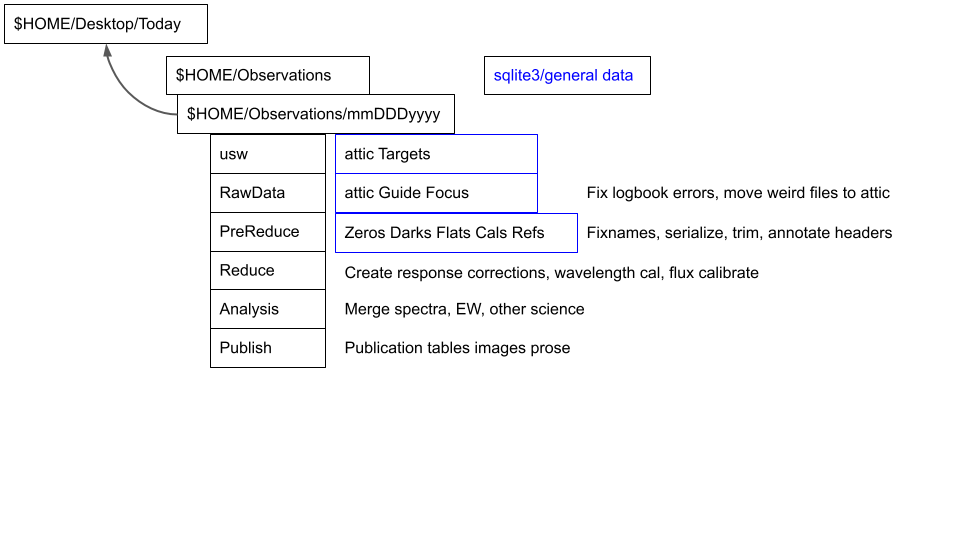
\includegraphics[width=.8\textwidth]{images/Overview1.png}
\caption{Basic Pipeline Steps} %% \caption{{\tiny{citation}}}
\label{figure:basicpipeline}
\end{figure}

\clearpage

\setcounter{section}{0}

\ifx\documentisdraft\drafttest
\linenumbers    %%%%%%%%%%%%% DRAFT
\fi

\clearpage
\pagenumbering{arabic}
%% \fancyfoot[ELF,OLF]{Go to: \hyperref[sec:contents]{Contents}}
%% \fancyfoot[ERF,ORF]{Go to: \hyperref[sec:index]{Index}}
%% \fancyfoot[ECF,OCF]{Page \thepage}

\fancyfoot[LF,OLF]{Go to: \hyperref[sec:contents]{Contents}}
\fancyfoot[RF,ORF]{Go to: \hyperref[sec:index]{Index}}
\fancyfoot[CF,OCF]{Page \thepage}


\section*{Overview}

This document refers to the new IRAF/Pyraf Noirlab 2.18 supported
Pyraf3 : \url{https://iraf.noirlab.edu/} and
\url{https://github.com/iraf-community/pyraf}.

The document covers details system setup for observing and reduction.
We are using a Raspberry Pi/libindi/Ekos for managing cameras and
other details. Once data is captured it is quickly copied to a more
stable platform for backup and reduction. We have IRAF/PyRAF installed
on the RPi to facilitate focus and quick tests of the images.

IRAF/PyRAF is considered a terminal based ``command line
environment'', a very flexible way to use small programs to achieve
large goals. GUI environments restrict users to 'canned' logic. Many
people are uncomfortable with command line work. It requires learning,
practice, and frequent use to maintain a fine edge needed for scientific
data reduction.

This \dhl{Bon Mots} document represents many tricks that one may use
to avoid editing temporary files by hand and to provide an audit trail
for projects.

Go to Section \ref{sec:complexexample} and briefly ponder the code with an
eye towards: ``What is this person thinking!''.

\section{Typography} \label{sec:Typography}

The typographic conventions used in these notes.

Here \llbox{k} means hit the ``k'' on the keyboard. 

\subsection*{Text}

The document uses \dhl{color} to make something \dhl{interesting},
stand out from the text.

\subsection*{Examples}

Examples, in general, state a \dhl{Goal}, the statement of the
\dhl{example}, and \dhl{Prose} to describe the 'thought model' or a
statement about takeaways from the example, and where needed some
exercises. These are presented in this format:

\begin{quote}
\goal Demonstrate a goal. Yes this example was a goal.\\ \example Give
an example of some syntax.\\ \prose Hey, put a linguistic pattern into
your ``thought process'' for that syntax.\\ \exercise[-a] Pick up your
pencil and start your notebook! \\ \exercise[-b] Time to stand for a
minute. \\ \takeaway Tie the thought process to a concrete goal and
example and begin documenting and checking your work.
\end{quote}

\subsection{Margin Annotations}

There are places in the notes where margin annotations are used
to draw attention to something important. In some cases this will
be a note to the author to add/clarify a section of text. Usually
more information may be found in the End Notes section of the document.
\ltodo{Example of Margin Note}{Added a note to demonstrate the note process.}

\subsection{Index}

This document is written in \LaTeX. The \LaTeX environment permits developing
and maintaining a set of bibliographic references, a great index and glossary. 

\section{The Unix and the Data ``Big Picture''}

This document is centered around the Ubuntu 22.04 LTS release using
the NOIRlab IRAF/PyRAF 2.18 pagkage. It offers a paradigm developed
over years of working with IRAF. This leverages Unix. The astronomy
community uses Apple Mac computers that still retain enough about Unix
to allow easy porting of IRAF and friends to that platform, even the
Apple Mx processors.

Win1X requires a VirtualBox (the Microsoft HyperV does not work well
enough).  The client operating system installed in the Virtual box may
be Fedora (the community version of Red Hat Enterprise Linux or RHEL).
This allows installing ESO packages that leverage the RHEL environment.
\textbf{Note}: Some AMD processors will not run hypervisors.
\index(RHEL!ESO) \index{RHEL!Win1X} \index(VirtualBox)

In Unix everything is a 'file'. Programs should be small, perform a
duty and do it well, permit some options. A program takes input from
``standard-in'' (\dhl{stdin}), does its work and puts its output to
``standard-out'' (\dhl{stdout}). Any errrors are reported via
``standard-err'' (\dhl{stderr}). Unix uses a device called a \dhl{pipe}
to send the output from one program into the stdin input of another.
Thus programs can be linked together on one line. 

OK, some programs are huge, and this paradigm does not necessarily
apply. But all the basic Unix utility programs like \dhl{ls}, \dhl{find},
\dhl{grep} etc work this way.

Changing from a GUI paradigm to a command line paradigm is one of the
hardest things for many reading these notes to do.

The Unix philosophy set forth by Ken Thompson, as documented by Doug
McIlroy \cite{McIlroy1978,McIlloryPhilosophy}:

\begin{quote}
Make each program do one thing well. To do a new job, build afresh
rather than complicate old programs by adding new "features". Expect
the output of every program to become the input to another, as yet
unknown, program. -- McIlroy
\end{quote}

GIUs are monolithic in design.\footnote{A GUI is a great way to encapsulate
a process where variation in the process is shuned and discouraged. Scientific
data is noisy and physics is opinionated -- this requires a careful attention
to detail not managable with GUI environments.}

One negotiates with Linux's root process to connect to the Linux
system, where the login process drops the user into a \dhl{shell}. There are
several shells to choose from -- here we will stick with \dhl{bash}
\index{bash}. \textbf{\emph{Note:}} \dhl{/usr/sh} defaults to an abbreviated shell
called \dhl{dash} on most Debian systems. \index{Unix Shell!intro}

\begin{quote}
``On a UNIX system, everything is a file; if something is not a file, it is a process.'' --
Machtelt Garrels, ``Introduction To Linux: A Hands On Guide''
\end{quote}

Peter Freeman \cite{freeman1975software} offered a model of a computer
(and a good operating system) as one of a \dhl{Processor},
\dhl{Memory} and \dhl{Transducer} (PMT) \index{computer!PMT}. The
processors today have less than one core to multiple cores, symmetric
arrays of cores and massively parallel cores.  Even the core of yore
is being supplanted by compute engines, the current popular one is the
GPU with $10^{\$}$ tiny cores.

Files are specialized and fall into classifications like: directories,
special files, links, sockets, named pipes.

There is only one file system and it starts at ``/'' or \dhl{root}.
We tend to think of files as residing on a disk drive. Multiple
drives, and their multiple partitions are simply ``mounted'' at
a location under the ``/''   root directory. Examples are
usually called something like /usr2. Disks on other machines
are usually found, conceptually as a sub-directory the /mnt directory.

\subsection*{The Shell ,``commands'', and Scripts}

The computer sees typed text as groups of characters separated by some
delimiter. Usually the delimiter is a combination of one or more
spaces and/or tab characters. These are called \dhl{whitespace}.

So all of programming takes a stream of complex symbols that, when
taken together, direct the computer to take some safe action. Linux
uses whitespace to set apart each symbol. 

Commands are designed to be typed at the keyboard and are usually
highly abbreviated. One of the handiest commands is \dhl{man}.

\example Use the ``\dhl{man}'' command \\
\prose Hey, what does the man (or ls or ln) command do?\\
\exercise Enter ``\dhl{man man}'' at the shell prompt.\\
\takeaway Read about how man works!\\
\exercise[-b] Enter ``\dhl{man ls}'' at the shell promot.\\
\takeaway Note: it says ``list directory contents'' so the abbreviation
of ``ls'' makes sense. It also offers up a myriad of options.\\
\exercise[-c] Try ``\dhl{ls -l}'' to see details of each file, one per line.\\
\takeaway A way to determine if files are normal files, directories or
links.

One of the oldest Unix commands is ``ls'' used to 'LiSt' directories and
their contents in interesting ways.

\section{Files and Directory Structure}

IRAF/PyRAF 2.18 is installed at a system level, and customized for each user.
The \dhl{mkiraf} command will create a {\textasciitilde}/.iraf directory.

IRAF uses two key files: \dhl{login.cl} and \dhl{loginuser.cl} to select from a myrid
of options and packages one will use for the tasks at hand. The \dhl{login.cl}
file now resides at \dhl{/etc/iraf/login.cl}. The loginuser.cl is located
at {\textasciitilde}/.iraf.loginuser.cl -- this is the file you change.
\textbf{\emph{Note}}: a single line with the word ``keep'' is required at the bottom
of this file.

The loginuser.cl file may be used to add your own special on-off commands,
and to leverage \dhl{foreign} tasks (usually other handy programs on the
path). \index{IRAF!foreign tasks}

Each IRAF task has a set of parameters, managed in the {\textasciitilde}/.iraf/uparam
directory. 

\textbf{BEWARE}: IRAF tasks are ``sticky''. When you change something it remembers the new
thing. The IRAF command \dhl{unlearn <task>} will cause the task to revert to
its defaults. \index{IRAF!sticky}

Other files:

\vspace{-.15cm}
\begin{enumerate}\addtolength{\itemsep}{-0.5\baselineskip}
%\setcounter{enumi}{N}
   \item  {\textasciitilde}/.bashrc, include your own {\textasciitilde}/.iraf-aliases
   \item  login.cl  - traditional configuration, don't edit this one.
   \item  loginuser.cl - configuration to users special taste.
   \item  pyraflogin.py - while not official has handy python functions
   \item  home\$/uparm - where the system keeps parameter files.
\end{enumerate}

\subsection{Directory Layout}

There are two quintessential things about data: 1) preserve the data
and 2) be able to audit processing of the data.

The most important thing is the preservation of the data. Backup,
Backup and Backup again. Then make a copy. It is best to save data on
multiple machines, or to the cloud. Google Drive (and other places)
offer 5TB of data storage for a quite reasonable fee.

All camera data consists of \dhl{16-bit unsigned ADU} values per pixel from
the camera. It is not necessary to change and/or archive raw data with
float values. The QHY600M images are 9600 x 6433 x 2 bytes of image,
roughly 13e6 bytes. Therefore 5TB of disk space will hold roughly
380,000 images. At 3 images per minute for an 8 hour night you get
2400 days of observations for 5TB of disk storage. That's 12 years in
practical terms. However, transferring these images over the net is a
problem.

% (iv (setq tmp (* 9600 6433 2)))    123513600  
% (iv (setq tmp (/ 5e12 13e6 )))    384615
% (iv (setq tmp (/ 384615 (/ 1440 3 3) 200 )))   12     2403

The \dhl{{\textasciitilde}/Desktop} directory allows software acquisiton software to be
configured once. Each night should be copied and archived. 

\begin{quote}
\begin{figure}[h!]
\dirtree{%
.1 {/home/user}.
.2 Observations.
.3 usw  - target lists, cl, notes, other generic things.
.3 ddMMMyyyy  - Date of sunset at Observatory.
.4 usw  - target lists, cl, notes, other generic things.
.4 RawData  - data: warts, blisters and all made read only.
.4 PreReduce  - copy RawData, and work here.
.4 PreAnalysis - pick up analysis for files.
.4 Reduce - Major IRAF/NonIraf reduction.
.4 Analysis - Major IRAF/NonIraf analysis.
.2 Desktop.
.3 Today - where all ``tonights'' observations go.
}
\label{figure:dirlayout}
\end{figure}
\end{quote}


The directory \dhl{usw} is used in lieu of etc. It is the German language
way of saying the samething - \dhl{und so wieder} ``and so again''.
In Unix \dhl{etc} contains loosely related information. For example
puruse \dhl{/etc}, where the system keeps configuration information
of a global level. It is so overloaded something unique is desired.

With this layout, the \dhl{{\textasciitilde}/Observations/usw}
directory contains side files of importance your overall personal
observing strategy. Files, like ds9 region files, special catalog
files general tools etc are stored here. Make subdirectories that
hold common information for different sites or instruments. Copy
those data into a nightly structure as needed.

Data is taken at night. Use dates that reflect the date of sunset
at the site where the data were obtained.

Using the KStars/Ekos/libindi, running on a Raspberry Pi for example,
or a local machine you may want a \dhl{{\textasciitilde}/Desktop/Today} directory
for each night's observing run. In this way the capture/observatory
software does not have to be configured each night. That export directory
remains the same. At the end of the night, simply rename the directory.

Date formats may be confusing, and subject to a computer's LOCALE
subsystem Nobody can make their minds up about date formats.

\centerline{{\huge{{\color{darkred}{SO! SPELL THE DATE OUT!}}}}}

The \dhl{ddMMMyyyy} directory uses the 1 or 2 digit day of month,
followed by the text abbreviation of the month, followed by a 4-digit
year (lets don't play Y2K again). 

This format makes the shell's text completion a quick way to move around.
Text completion involves typing a few starter characters of the file/directory
name then hit the tab. It will advance to the next non-unique thing.

Underneath \dhl{ddMMMyyyy} is the usw directory for tonight's work. The
target list, special catalog file of reference stars etc, the scheduler's
input. Here we store the \dhl{reduce.cl} or \dhl{reduce.py} script
template to be developed for these particular data.

The RawData/PreReduce/PreAnalysis/Reduce/Analysis directories are
cascading stages of data. You may use an \dhl{attic} directory where
to sideline unrelated or terrible images.

You can automate file reduction by using sub-scripts/tasks within the
melange of IRAF/PyRAF/bash/python/whatever language programs and then
leveraging Python and cl into making a
\dhl{OBSERVATION/usw/reduce.pyraf}\index{reduce.cl}
script\index{reduce.pyraf} script for the data. Save this as a template in
the general \dhl{usw} directory, and copy in to each observation's repository.
Detailed example is in Appendix \ref{sec:ReducePyrafControlFile}.

At this time PyRAF (a mix of ecl and Python) does not act well as a
``script'' due to the hack that adds ecl syntax to the GNU runline command
input. It uses the raw input directly and side-steps \dhl{stdin}. This
violates the Unix philosophy of each program should take its input from
stdin, process its results and put the results into stdout.  This
allows one to pipe programs together to achieve an ultimate goal.

Scripts may be written in the \dhl{.cl} language (really ecl or extended cl),
actual PyRAF (\dhl{.pyraf}), or hacked into PyRAF with the \llbox{!}
cl prefix as you go along.

\textbf{\emph{Note}}: The \dhl{.pyraf} scripts blend python and PyRAF together.
See the complicated example of how to deal with APO NICFPS camera
images.

\section{Critical First Steps}

It is critical you properly install the IRAF/PyRAF3 packages. This
release looks for a {\textasciitilde}/.iraf directory that may not be fully integrated
into the rest of IRAF.

You may make a soft link of \dhl{\home/iraf} to \dhl{\home/.iraf}:

\dhl{ln -s \home/iraf \home/.iraf}

The document will continue to refer to \dhl{\home/iraf} as the base
of the IRAF package. 

It is important to use a \dhl{~/iraf/loginuser.cl} file with task
aliases foreign and tasks.\index{tasks!aliases} \index{tasks!foreign
  tasks}

One way to make things simple is to create a bash alias for pyraf that:
\vspace{-.15cm}
\begin{enumerate}\addtolength{\itemsep}{-0.5\baselineskip}
%\setcounter{enumi}{N}
   \item   uses xdotool to change the color of the window's background
   \item   update the PATH and PYTHONPATH to access all the special files you use
   \item   run the system pyraf (note the /usr/bin path is prefix is necessary) 
 with the ``-s'' switch for ``silent'' start.
\end{enumerate}


\begingroup \fontsize{10pt}{10pt}
\selectfont
%%\begin{Verbatim} [commandchars=\\\{\}]
\begin{verbatim} 
alias pyraf="xdotool key shift+F10 r 1;\\
  export PATH="/usr/local/bin:$PATH"; export PATH="/usr/local/astrometry/bin:$PATH";\\
  export PYTHONPATH=$HOME/.iraf; export PATH="$HOME/.iraf/smtsci/bin:$PATH";\\
  /usr/bin/pyraf -s;"
\end{verbatim}
\endgroup
%% \end{Verbatim}

\subsection{IRAF/PyRAF Tasks and Packages}

IRAF, from ye-olden times, uses \dhl{packages} containing help text
and parameter files to hold values from run-to-run together with the tasks'
executable code.
\index{IRAF!tasks} Tasks are ``programs'', usually written in FORTRAN
or in cl proceedural code. Some are written in C/C++.

\dhl{BEWARE}: IRAF is \dhl{sticky}! It retains parameter values from
run-to-run that can perpetuate errors. Review all the parameters to be
sure your reductions are proper. These values are stored in the
\dhl{~/iraf/uparm} directory.

Tasks are built into IRAF/PyRAF but are only loaded once. Each time
they are used -- they are in memory and already part of the CPU thread
you are using. Thus they very fast. Using \llbox{!} shell-escape or a
\dhl{\$foreign} task causes Unix to create a new heavy-thread with
significant overhead (especially in a loop).

IRAF has a habit of loading images into memory and keeping them there.
Some tasks will modify the in-memory image but not write it back to
the disk. Work may be lost. See Section \ref{sec:FITSFiles} for quick
details.

IRAF has a neurotic habit of \dhl{sometimes} adding an extent to
certain FITS files! This is the case with master darks and flats
and a handful of other operations.

It is best to develop your \dhl{reduce.pyraf} script in an editor, one line
and step at a time, then cut/paste edited lines at the interactive
prompt. When you make a mistake -- and you will -- you can start over
with a fresh copy of data and stop short of the mistake. Pick up and
go again.

\subsection{Full On Python Hacks}

\example Python's \dhl{import iraf} statement allows for operations like: \\
\prose I want to use IRAF's imstat command to get a binary value, assign
the value to my python variable. \\
\exercise Enter: \\
{\color{verbcolor}{
\begingroup \fontsize{10pt}{10pt}
\selectfont
%%\begin{Verbatim} [commandchars=\\\{\}]
\begin{verbatim} 
mymean = float( iraf.imstat(images='*fits',fields='mean',format=iraf.no,Stdout=1)[0])
\end{verbatim}
\endgroup
%% \end{Verbatim}
}}

\takeaway The task has a pythonic wrapper, contained in the iraf.py
module's namespace.  It needs a list of files, we only want the one
field \dhl{mean}, we do not want the headers (format=iraf.no). The
phrase Stdout=1 (note capitalization) returns the text as a string
rather than printing on the terminal. But! The string is actually an
array, so we want the first bit. But! that bit is a string, and we
need to convert to binary with the \dhl{float} python function.

where \dhl{mymean} is now a proper python float. Yes, convoluted, but
its buried in a scrip and available for your use. \index{Stdout}

\subsection{Task Parameters}

Always be aware of the:
\vspace{-.15cm}
\begin{enumerate}\addtolength{\itemsep}{-0.5\baselineskip}
%\setcounter{enumi}{N}
   \item    ~/iraf/uparm directory
   \item    lparm <taskname> command to list parameters.
   \item    \dhl{unlearn <task>} command.
   \item   help <task> and look at the see also part at the bottom.
\end{enumerate}

\section{Goals}

The main goal of scripting is not the script, it is the result. Good
data results do not come from good scripting -- but come from good
planning, good execution of the plan and attention to configuring
your tools.


\subsection{Things to remember}

IRAF \dhl{cl} morphed into PyRAF \cite{2006hstc.conf..437G} to allow a more
powerful \dhl{cl} by hacking the Python \dhl{readline} subsystem. The
grammar of python was altered to allow for a ``direct entry'' of most older
\dhl{cl} commands. Direct access to the underlying tasks was
accomplished with a ``cythonic'' interface into underlying code. An ``iraf''
module was added to support programming calls to IRAF tasks and using 
a special Python \dhl{keyword} argument Stdout to return output as a string.
Parsing this string with python allows chaining \dhl{cl} commands together
for a goal.

A tremendous amount of power is available for you to mix and match to meet
your specific needs. 

\subsection{Observation Directory}

One can not expect proper structure by simply importing a night's
observations, warts blisters and all. Files will be scattered all
over, mis-named, bad headers, useless(!), and other oddities. But copy
the data into date/RawData. See directory layout table \ref{figure:dirlayout}

Open date/usw/reduce.cl in your favorite editor. Anything you want
to type into PyRAF -- type it into the reduce.cl file. Then cut/paste
the command to PyRAF. This means when you make the mistake -- you
can remove the last line, save the reduce.cl file, and rebuild
to that point. Yes, some interactive things will or may happen.
Try not to make too many mistakes.

\vspace{-.15cm}
\begin{enumerate}\addtolength{\itemsep}{-0.5\baselineskip}
   \item   cd ~/Observations
   \item   mkdir 22Feb2022 \# date of sunset at the observatory
   \item   cd 22Feb2022
   \item   mkdir -p Plan RawData PreAnalysis Analysis Publish usw
   \item   mkdir -p PreAnalysis/{Bias,Darks/{s300,s3},Flats,Comps} \# prior knowledge
   \item   cd RawData
   \item   cp -pr /mnt/NAS/22Feb2022/* .  \# copy the raw data
\end{enumerate}

Now the plan for observations and initial PreAnalysis results is in 
place. The \dhl{usw/reduce.cl} script is the key. 

Good observations are the result of good planning. Make the list of targets,
determine offsets and guide stars, create a ds9 region file in ICRF WCS
coordinates for the field of view and possible orientations of the instrument.
If possible download the preparation package from the observatory and take
time to prepare. \index{planning}

\begin{figure}[h!]
\centering
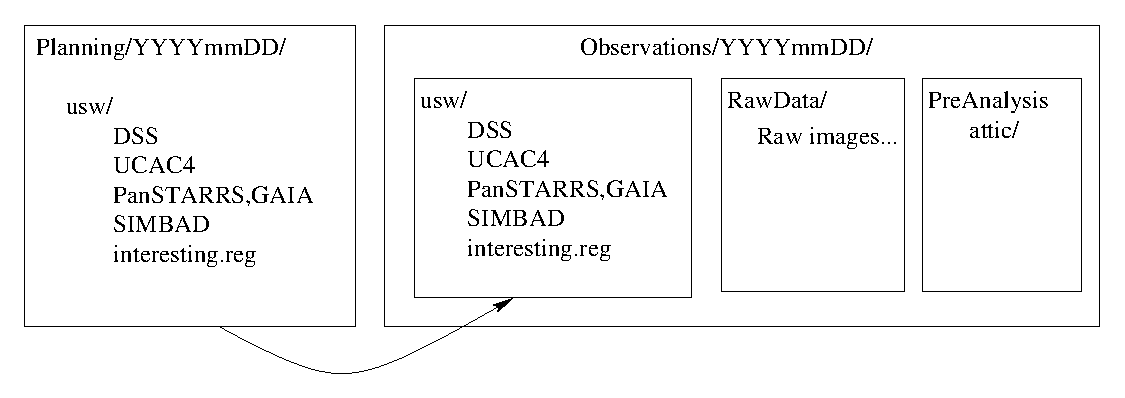
\includegraphics[width=.4\textwidth]{images/Overview.eps}
\caption{The observations directory was in place with the plan.
Load up the raw images. Then copy raw data to pre-analysis.} %% \caption{{\tiny{citation}}}
\label{figure:GoalsOverview}
\end{figure}

\clearpage
\subsection{The main tricks}

Note: Unix files do not rely on their extensions. A Unix extension is a social
convention. Many authors use two files, like \dhl{in.txt} and \dhl{out.txt}.
They will use an editor to change the bits of one to another. 

I recommend using goofy file names, like \dhl{xxx} and \dhl{l.l}, when seen
they may be removed. The filename \dhl{l.l} is real easy to type because
the \llbox{l} and \llbox{.} are right next to each other!

The \llbox{/}\llbox{/} sequence is the cl concatenation operator, used to
join two strings without intervening whitespace.

Instead of having the input files in in.txt, then editing to make unique
output names -- simply prepend a string, with some meaningful context
to the @file. 

The order of operations may be to
\vspace{-.15cm}
\begin{enumerate}\addtolength{\itemsep}{-0.5\baselineskip}
%\setcounter{enumi}{N}
   \item   t\_ trim a file.
   \item   c\_ cosmic ray removal
   \item   z\_ to zero correct
   \item   d\_ to dark correct
   \item   f\_ to flat a file
\end{enumerate}


etc. data.fits, after processing may be \dhl{f\_d\_z\_c\_t\_data.fits}.

So PyRAF has several tricks up its sleave:
\begin{itemize}
\addtolength{\itemsep}{-0.5\baselineskip}
   \item   It can act like a basic ``calculator'' just by typing standard python at the
PyRAF command prompt. Remember to ``import'' packages like math and numpy.
   \item It works with list of files. These are refered to as ``list''
     or ``at'' files. They are like {\color{verbcolor}{\verb#@l.l#}}
     where the file ``l.l'' has a list of filenames -- one per line.
   \item You can take the files in ``l.l'' and produce new files with
     the same name but prepend a clause to the
     filename!\\ \textbf{E.g.:}
     {\color{verbcolor}{\verb#imarith @l.l - zmaster.fits z_//@l.l#}}\\ will
     subtract the zero master from each file in ``l.l'' and make a
     corresponding {\color{verbcolor}{\verb#z_filename.fits#}}.
\item PyRAF is a a replacement for {\color{verbcolor}{\verb#cl#}} (actually
ecl). You can loop {\color{verbcolor}{\verb#.cl#}} commands together
with bash commands into the mix to do work using:\\
{\color{verbcolor}{\verb#cl < ~/iraf/fit2fits.cl#}} to bring a Vendor's
fit format to the PyRAF standards.
\end{itemize}

It has a few oddities, inherited from the ecl lashup of the Pythonic 'readline' hack,
ripped from a \dhl{reduce.cl} script:

\vspace{-.15cm}
\begin{enumerate}\addtolength{\itemsep}{-0.5\baselineskip}
   \item Oops! Its Python 2.7 so write helpers like \dhl{trim} and
     \dhl{fitsls} accordingly.
   \item   Most of the IRAF \dhl{cl} commands work
   \item   \dhl{set OBSROOT=/home/me/Observations/23Feb2022}
   \item   \dhl{set OBS=OBSROOT\$/PreAnalysis}
\end{enumerate}

The IRAF command \dhl{chdir} \index{cl!chdir} changes directory while respecting
the IRAF use of iraf-environment variables.

You can escape to bash by starting the line with a bang (!). This
allows developing handy bash scripts to store in iraf/bin.

\clearpage

\subsection{System Setup}

I presume the use of the Ubuntu 22.04 Linux distribution from Canonical\texttrademark.

%% Under Microsoft Windows\texttrademark Pro, there is a system called \dhl{Hyper-V}.
%% It is very ``light-weight'' virtualization layer for Windows that permits
%% the seamless of an essentially containerized Ubuntu 22.04 + anaconda and other
%% Linux based tools while maintaining contact with the Windows file system,
%% the network etc. \index{Windows!Hyper-V}.

%%Under Linux you are running Linux anyway.
MacOS is very Linux like, even on their M1 processor series.

Install the Anaconda package without the Navigator. This brings in
a massive amount of power, including Astropy \cite{astropy:2013} \cite{astropy:2018}
\cite{astropy:2022}.
\vspace{-.15cm}
\begin{enumerate}\addtolength{\itemsep}{-0.5\baselineskip}
   \item    Necessary:
\vspace{-.15cm}
\begin{enumerate}\addtolength{\itemsep}{-0.5\baselineskip}
   \item    Ubuntu 22.04/Mac OS + many apt-get packages
   \item    Anaconda (Python 3+)
   \item    Astroconda PyRAF recipe (a python2.7 env)
   \item    Ubuntu aptitude iraf/pyraf packages
   \item    Sextractor
   \item    Current SAOImage/ds9
   \item    Current Astrometry.net + 4200 and GIAI data
   \item    Fitsverify \cite{fitsverify-1}
   \item    GitHUB sasiraf package (currently private contact author.)
\end{enumerate}
   \item    Optional
\end{enumerate}

\subsection{Unix\texttrademark Aliases}
A few aliases need to be setup.

\ltodo{Add Aliases}{Update/add aliases for bashrc file.}

\begin{figure}
{\color{darkred}
\begingroup \fontsize{10pt}{10pt}
\selectfont
%%\begin{Verbatim} [commandchars=\\\{\}]
\begin{verbatim} 
function pyraf  { #export PYTHONPATH=$HOME/iraf;
                  export PATH="/home/wayne/anaconda3.8/envs/geminiconda \\
                     /bin:$HOME/iraf/smtsci/bin:$PATH"; (folded line)
                  source activate geminiconda;
                  xdotool key shift+F10 r 6;     # change terminal color
                  $HOME/anaconda3/envs/geminiconda/bin/pyraf -s $*;
                }
\end{verbatim}
\endgroup
%% \end{Verbatim}
}
\caption{An entry into the aliases file, using the Gemini pyraf installation.}
\label{fig:geminialias}
\end{figure}

This is a little-bit complicated:
\vspace{-.15cm}
\begin{enumerate}\addtolength{\itemsep}{-0.5\baselineskip}
   \item   The PYTHONPATH allows pyraflogin3 to be imported after start.
   \item   This assumes \dhl{~/iraf/pyraflogin.py} is present.
   \item   The function in figure \ref{fig:geminialias} tells Anaconda to activate
     the geminiconda environment
   \item   The xdotool allows the color of the terminal window to be changed.
   \item   PyRAF is then started, the \dhl{-s} switch is quiet about packages loaded.
   \item When pyraf starts, it loads \dhl{login.cl} which in turn
     loads my \dhl{loginuser.cl} scripts.
\end{enumerate}

\subsection{Initialization files}

PyRAF uses \dhl{~/.iraf/login.cl} to manage system level commands and should
not be edited -- except to ensure that \dhl{cl < "home\$/iraf/loginuser.cl"} is
enabled. Edit the \dhl{loginuser.cl} file and pile changes.
 \index{Initialization!login.cl}
\index{Initialization!loginuser.cl}

A special \dhl{~/iraf/pyraflogin.py} file can 'extend' the Python
environment.  A sample file is available with this package. It
requires the special alias to start PyRAF. It adds simple
\dhl{matplotlib} plotting and some handy fixer-upper functions. See
that package for documentation. \index{Initialization!pyraflogin.py}

\subsection{Initial Steps}

This process uses a user-defined  directory structure as shown in
figure \ref{figure:basicpipeline}. 

The main steps are:
\vspace{-.15cm}
\begin{enumerate}\addtolength{\itemsep}{-0.5\baselineskip}
   \item   Layout basic directory structure:


   \item  Add a few toplevel soft-links for non-sentient file browsers.
\dirtree{%
.1 \$HOME/.aaatoday linked to \$HOME/Desktop/Today.
.1 \$HOME/.aaareduce linked to current working reduction.
}

   \item   Planning - load up the \dhl{\$HOME/Desktop/Today/usw} directory with
FOV files, and anything related to observatory etc.

   \item   Observe
   \item   Move dhl{\$HOME/Desktop/Today} to dhl{\$HOME/Desktop/Observations/mmDDDyyy}
date of sunset at the observatory of the instrument.
   \item   Make a safe backup.
   \item   Start the process of reducing the data.
\end{enumerate}

The script provides the audit trail you used. Modify this for each
instrument setup, and for each filter type etc.  Essentially the same
for spectroscopy -- just watch the statistics sections.

You may not need darks, and the flats will be different.

When, not if, you mess up you can delete the PreAnalysis directory, fix
the above script, and start over. As you move deeper into the file
processing, the script becomes more valuable.


\clearpage
\subsection{PyRAF Calculator Mode}

\goal Demonstrate borrow Pyraf as a calculator within PyRAF. Determine
the mean plus 3 times the standard deviation for a limit.

\example 
{\color{verbcolor}{\verb#imstat zmaster.fits fields=mean,stddev#}} \\
you find the mean is 346 and the stddev is 47.

\exercise How many pixels in the zero master are 3 or 5 $\sigma$ above
the mean?

{\color{verbcolor}
\begingroup \fontsize{10pt}{10pt}
\selectfont
%%\begin{Verbatim} [commandchars=\\\{\}]
\begin{verbatim}
from astropy import fits  # DO THE IMPORTS ONCE
import numpy

f = fits.open('zmaster.fits')    # open the fits file as a cfitsio like
d = f[0].data   # get the data   # structure and just grab the data.
# using some python magic!
(mean,stddev) = map(float,
                   iraf.imstatistics(Stdout=1,fields='mean,stddev',
                      images='zmaster.fits',format=iraf.no)[0].split())
len(d[d> mean + 3.0*(stddev)]) # 25729 pixels matched this example
len(d[d> mean + 5.0*(stddev)]) #  1220 pixels matched this example
f.close()
\end{verbatim}
\endgroup
%% \end{Verbatim}
}


\prose Hey, we're PyRAF, a pythonic interpreter -- so lets really use
Python.  The imports are used to get the modules/functions we
need. The fits.open gets the FITS file open for business; we grab just
the image data as a numpy array of shape
{\color{verbcolor}{\verb#NAXIS2,NAXIS1#}} (switched(!), numbered from
zero now and the data will have overscans if present!) using
{\color{verbcolor}{\verb#d = f[0].data#}}. The
{\color{verbcolor}{\verb#iraf#}} is imported by virtue of we're PyRAF;
the {\color{verbcolor}{\verb#imstat#}} is run as a python function
using {\color{verbcolor}{\verb#iraf.statistics()#}}.  The
{\color{verbcolor}{\verb#Stdout=1#}} tells the task to return the
output not send it to the terminal. The
{\color{verbcolor}{\verb#format=no#}} tells the function to omit the
usual header text etc, and just return the two values requested with
the {\color{verbcolor}{\verb#fields="mean,stddev"#}}.  The output is
one string with two ASCII numbers. These are split into an array, then
the {\color{verbcolor}{\verb#float#}} function converts the strings
into actual numbers -- returned as the tuple
{\color{verbcolor}{\verb#(mean,stddev)#}}.

\subsection{Using Numpy Arrays}
%HEREHEREHERE

Numpy arrays follow the ``C'' indexing scheme, which is ``ordinal'' in nature
(starting with zero). For an (X,Y,Z) index -- the array is referenced \dhl{backwards}:
myarray[Z][Y][X]. This differs from the FORTRAN convention for arrays, ``cardinal''
in nature (counting from 1).

FITS images are stored in FORTRAN order, and in Big Endian format. This makes
difficult for Intel architectures.

This is critical. Data are written into FITS images in so-called \dhl{Big-Endian}
fashion. In Jonathan's ``Gulliver's Travels'', a fictional character encounters
a culture in heated conflict over weather or not one should crack open an
egg on the little end or the big end. Computer aritectures are conflicted on
how to store a larger value, say an integer that spans more than one byte
into a linear address space. Decisions (bad perhaps) were made to store
a 16-bit integer with the byte containing least significant digit first.
The word oxBO is stored with the 0 first then the 0x0B. This was to make
a very early machine fast at ++value operations! We're stuck with that decision
since.

The real issue boils down to the Bad Thing\texttrademark practice of
``type punning'' whereby a block of data in ``Endianess Be Damed''
format is read into memory, then attempts to access it as though it
had the right byte order results in catastropy when data is exchanged
between the types of architectures.

Intel processors are ``Little Endian'' where processors like the Motorla
68000 were ``Big Endian''. 

Data are stored as arrays, with astropy.fits.io open command setting the
data[0] extent as a pythonic numpy array. So the indices are a bit backwards
The fits header would read something like:

\begingroup \fontsize{10pt}{10pt}
\selectfont
%%\begin{Verbatim} [commandchars=\\\{\}]
\begin{verbatim} 
NAXIS  = 2
NAXIS1 = 2048
NAXIS2 = 512
\end{verbatim}
\endgroup
%% \end{Verbatim}

To store a 2D image array. This is ment to denote an image that is 2048 wide and 512
tall. 

\ltodo{numpy vs FORTRAN}{Get into index details.}


The next bits use numpy arrays. Here we use the conditonal indexing
mode common to numpy arrays to get all the pixels that match
expression of the value > the
{\color{verbcolor}{\verb#mean + n times stddev#}}.

Need a ``Quick Calculation'' to find the center of an image to
use as a ``statistics section'' for normalizing?:

{\color{verbcolor}
\begingroup \fontsize{10pt}{10pt}
\selectfont
%%\begin{Verbatim} [commandchars=\\\{\}]
\begin{verbatim}
imhead zmaster.fits   # result is 'zmaster.fits[1368,1364][real]:'
# half size? pick up the [NAXIS1,NAXIS2] from abbreviated imhead result...
(1368//2, 1364//2)   # returns tuple (684, 682)  the '//' is integer divide.
print "[%d:%d,%d:%d]" % (1368//2 - 50, 1368//2 + 50, 1364//2 - 50, 1364//2 + 50)
# [634:734,632:732]  Et Viola! A handy center stat section for normalizing!
\end{verbatim}
\endgroup
%% \end{Verbatim}
}

Make your own functions! Then imexamine -- the comp star and the target star.

{\color{verbcolor}
\begingroup \fontsize{10pt}{10pt}
\selectfont
%%\begin{Verbatim} [commandchars=\\\{\}]
\begin{verbatim}
import math    # DO THIS ONCE
def mag(compmag,compflux,observedflux):
   return -2.5(math.log10(observedflux / compflux) + compmag
\end{verbatim}
\endgroup
%% \end{Verbatim}
}

\exercise Correct for background.

\section{Getting Started}

Configure the system. Copy the login.cl to ~/.iraf. Copy loginuser.cl script
to ~/iraf. \textbf{\emph{Note}} One has a hidden-file dot.

Add the .iraf.aliases file to \dhl{\$HOME} directory and if you like, add it to
the \dhl{\$HOME/.bashrc} file.

Start PyRAF in one window and start Editor in another window. I
recommend emacs or Sublime Text as editors -- they are GUI
oriented. Remember all things have a learning curve.

Why we use the vi editor. Vi is the ``\dhl{Vi}sual Editor'' that sits
on top of a powerful albeit basic Unix editor ``\dhl{ed}. The \dhl{ed}
editor is the basis for the \dhl{sed} the Unix stream editor. Regular
expressions (think wildcards) are very sophisticated and turn up all
over the Linux/Unix system. They are worth the effort to learn. The
``re'' of the grep program (\dhl{g}lobal \dhl{re}gular expression
\dhl{p}rint) program obviously makes heavy use of regular expressions.

The very basic Linux commands are:

\begin{table}[h!]
\centering
\begin{tabular}{| l | l |}
\hline
Command  & Basic Action   \\
\hline
cd    & change directory    \\ 
ls    & list files     \\ 
pwd   & print the current working directory    \\ 
cat   & \dhl{concatenate} file(s)    \\ 
less  & view content of a file    \\ 
man   & the Manual -- print details of a command \\ 
which & show where on PATH an executable is \\ 
rm    & remove files and directories. \\
%% ones-based: \cline{a-b}
\hline
%%\DeleteShortVerb{|}
\end{tabular}
%%\end{minipage}    %% for footnotes  r@{.}l 
\caption{Very Basic Unix Commands}
\label{table:VeryBasicUnixCommands}
%%} % end small etc
\end{table}


\subsection{Very Basic PyRAF commands}

\begin{table}[h!]
\centering
\begin{tabular}{| l | l |}
\hline
Command  & Use   \\
\hline
cl            & run the cl editor                            \\
epar          & edit parameters/launch task                  \\
hedit         & fast/dirty header editor                     \\ 
imhead        & list the header values for a file            \\ 
hselect       & select values from headers                   \\ 
imexamine     & all manor of ways to view images             \\ 
apall         & reduce a spectrum image                      \\ 
identify      & identify spectral lines assign wavelenghts   \\
dispcor       & apply identify results to science spectrum   \\
splot         & view/analyze reduced spectrum                \\ 
imstat        & print mean,min,max,std etc for set of images \\ 
%% ones-based: \cline{a-b}
\hline
%%\DeleteShortVerb{|}
\end{tabular}
%%\end{minipage}    %% for footnotes  r@{.}l 
\caption{Very Basic IRAF/PyRAF commands}
\label{table:VeryBasicIRAF/PyRAFcommands}
%%} % end small etc
\end{table}


\section{Working on subsets of files.}

IRAF uses ``list files'' denoted \dhl{@list.txt}. The \llbox{@} key
as the first character of the filename tells IRAF to open that
file and take from it filenames -- one filename per line. This is
real handy.

Some documents have you make lists, then use an editor to change the
list as you go. They recommend filenames like mylist.txt. This is
cumbersome to type. Try using a simple name like \dhl{l.l}. Note the
\llbox{l} key is very near the \llbox{.} key! Handy to type.  If you
see the file \dhl{l.l} you know you can simply remove it.  The \llbox{!}
as the first character on a command line sends the rest of the line
to the local bash script. This escape mechanism allows you to use
all the power of Unix inside cl scripts.

The command \dhl{!ls -1 *Dar* > l.l} takes all filenames with Dar
in it and lists them out in lexicographical (sorted) order. Here
are some example of ways to build list-files.

{\color{verbcolor}
\begingroup \fontsize{10pt}{10pt}
\selectfont
%%\begin{Verbatim} [commandchars=\\\{\}]
\begin{verbatim}
!ls -1 *fits > l.l
cl < ~/iraf/crall.cl
# all the files are now c_<filename>

hselect c_*fits $I "IMAGETYP ?= 'Bias'"  > l.l
hedit @l.l IMAGETYP zero add+ show- ver- update+
!if test -e zmaster.fits; then rm zmaster.fits; fi  # bash to rm file if exists
imcombine @l.l zmaster.fits combine=median

hselect c_*fits $I IMAGETYP ?= 'Light'"  > l.l
hedit @l.l IMAGETYP object add+ show- ver- update+
imarith @l.l - zmaster.fits z_//@l.l
imarith z_//@l.l - dmaster.fits d_z_//@l.l
imarith d_z_//@l.l / flatmaster_SII.fits f_d_z_//@l.l

# files are now {\color{verbcolor}{\verb#f_d_z_c_filename.fits#}}
\end{verbatim}
\endgroup
%% \end{Verbatim}
}
This makes use of the fact that we can pile on prefixes to
processed files:

\begin{itemize}
\addtolength{\itemsep}{-0.5\baselineskip}
   \item   t - trimmed
   \item   c - cosmic ray reduced
   \item   z - zero subtracted
   \item   d - dark corrected
   \item   f - flat normalized
\end{itemize}

At the end, a flat-normalized file called {\color{verbcolor}{\verb#science.fits#}} will
have the name {\color{verbcolor}{\verb#f_d_z_c_t_science.fits#}}.

Lots of intermediate files lying around: Clean them up!

{\color{verbcolor}
\begingroup \fontsize{10pt}{10pt}
\selectfont
%%\begin{Verbatim} [commandchars=\\\{\}]
\begin{verbatim}
print "Remove residual files."
! (export LC_ALL=C; rm [a-z]_*fits 2> /dev/null;)
\end{verbatim}
\endgroup
%% \end{Verbatim}
}

\textbf{\emph{Prose:}} \textbf{\emph{Hey}} PyRAF send the line to bash; but! using a sub-shell
set {\color{verbcolor}{\verb#export#}} the {\color{verbcolor}{\verb#LC_ALL=C;#}}
shell variable to let bash actually use case sensitive wildcards. Then
{\color{verbcolor}{\verb#rm [a-z]_*fits 2> /dev/null;#}} remove the
file -- and in case there is some whining about the process, send the
whines to the bit-bucket ({\color{verbcolor}{\verb#/dev/null#}}).


\section{Observing}
PyRAF \index{PyRAF!Observing} is a useful tool for spectroscopy. Using
the imexamine command and the 'j' key: set the rplot to wider than a bright
line width. 

% HEREHEREHERE

\clearpage
\section{Overall Philosophical Approach}

This document covers a philosophy --- a set of general tools and
scripts to take and reduce data.

In this case some location like {\color{verbcolor}{\verb#/opt/myobs/iraf/#}}
or {\color{verbcolor}{\verb#~/iraf/#}} contains a number of small generic
{\color{verbcolor}{\verb#.cl#}} scripts to handle specific needs. These
are specific to certain conditions -- like a package that writes {\color{verbcolor}{\verb#.fts#}}
instead of {\color{verbcolor}{\verb#.fits#}} files. Routines to remove pesky
spaces that GUI users like to use; get rid of multiple ``dots''; plus signs
etc. 

\vspace{-.15cm}
\begin{enumerate}\addtolength{\itemsep}{-0.5\baselineskip}
   \item   Create a planning directory. Rename to Observations/directory
when the plan is executed.
   \item   Create a ``usw'' directory to hold the plan, collect pre-analysis information:
\vspace{-.15cm}
\begin{enumerate}\addtolength{\itemsep}{-0.5\baselineskip}
   \item   DSS image -- ds9 Analysis \menu Image Servers
   \item   Region files, catalog files for ds9 -- ds9 Region \menu Shape ...
   \item   Photometry reference stars --- ds9 Analysis \menu Catalogs \menu Database \menu UCAC4;
or with the Aladin application and TOPCAT make one the hard way. (PanSTARRS DR1).
   \item   Bibliographic information -- Browser and SIMBAD for the target(s).
   \item   Gather any existing bad pixel masks -- previous runs; observatory supplied files.
\end{enumerate}

   \item  Gather raw data --- stay up all night
   \item  Archive raw data as a RawData and make read only --- back to your {\color{verbcolor}{\verb#Observations#}} directory:\\
{\color{verbcolor}{\verb#(cd Observations/YYYYmmDD; mkdir -p RawData; cd RawData; rsync <from somewhere> .; chmod -w -R *#}}).
\end{enumerate}


\vspace{-.15cm}
\begin{enumerate}[resume]\addtolength{\itemsep}{-0.5\baselineskip}
   \item   Copy raw data to a PreAnalysis directory -- do not damage any
raw data whatsoever. Make the PreAnalysis files writable:\\
({\color{verbcolor}{\verb#cd Observations/YYYYmmDD; mkdir -p PreAnalysis; cd PreAnalysis; cp -pr ../RawData/* .; chmod +w -R .#}})\\
Clean data and make initial analysis files:
\vspace{-.15cm}
\begin{enumerate}\addtolength{\itemsep}{-0.5\baselineskip}
   \item   Fix the filenames --- {\color{verbcolor}{\verb#cl < ~sbo/iraf/fix_sbig.cl#}}
   \item   Fix the headers--- {\color{verbcolor}{\verb#cl < ~sbo/iraf/fix_headers.cl#}}
   \item   Trim (remember) overscan --- see above
   \item   Remove bad WCS especially from zero/dark/flats {\color{verbcolor}{\verb#cl < ~sbo/iraf/fix_sbig_wcs.cl#}}
   \item   Remove cosmic rays ---  {\color{verbcolor}{\verb#!ls -1 *fits > l.l#}}
followed by {\color{verbcolor}{\verb#cl < ~sbo/iraf/crall.cl#}}
\item Other basic reduction steps to be covered elsewhere:
\begin{enumerate}\addtolength{\itemsep}{-0.5\baselineskip}
   \item   Make any bad pixel masks 
   \item   Make master zeros and darks 
   \item   Make master flats 
   \item   apply zeros,darks,flats to science images
   \item   add new WCS or de-distort and add new WCS
   \item   extract photometry
   \item   combine images for deeper photometry
   \item   freeze this work
\end{enumerate}
\end{enumerate}


   \item  Copy the PreAnalysis data into an Analysis Directory.
(Any damage here is quickly recovered from PreAnalysis.)\\
{\color{verbcolor}{\verb#!(cd ..; mkdir -p Analysis; cd Analysis; cp -pr ../PreAnalysis/f_d_z_c_t* .)#}}
\end{enumerate}


A break down of the above steps reveals the need to make/use
certain scripts (some shown in red in context above):

\vspace{-.15cm}
\begin{enumerate}[resume]\addtolength{\itemsep}{-0.5\baselineskip}
   \item   Fix the filenames: remove dots, spaces, dashes other special characters.
   \item   Fix the headers: Observatory/Vendor non-IRAF keywords to IRAF
keywords; Very-Non-Standard keywords like PCOUNT and GCOUNT
   \item   Pinpoint is good enough for tracking (still takes a while to apply
and will fail) but is not accurate.
   \item   Single Pixel errors from cheap cameras, inevitable cosmic rays need
to be mitigated in raw zero, dark and flat frames.
   \item   Masks provide locations in pixel coordinates of defects that can ruin
the science.
   \item   Adding a new WCS will help to quickly align images. This may be enough
if there is no distortion, de-distort with flux conservation where possible.
\end{enumerate}


You can stop here and defer photometry to the analysis step. However,
you can extract photometry using sextractor and a few tricks.

Combining images is an art.


\textbf{\emph{Main goal:}} to develop a \textbf{\emph{compact}} set of
skills with Unix/Python/PyRAF/IRAF to create a
\textbf{\emph{collection}} of IRAF scripts to process images from two
cameras, three telescopes using vendor's software. In this sense,
``compact'' means: the basic IRAF commands; python, bash and Unix
tricks and commands; a basic use of SAOImage/ds9. A familiarity with
command line operations and vocabulary to support planning, executing,
reducing data and publishing photometic data. Summary: the course is
designed to introduce astrophysical hands-on research -- not the
tedious nature of the related software tools.

Examples, long and short, will provide an overview of all the weird/odd ways
Bash/IRAF/PyRAF and Python are used is in Appendix \ref{app:PutItTogether}.

\textbf{\emph{The Problem:}} PyRAF is a ``pythonic''
wrapper/controller of collection of IRAF tasks/commands that in turn
are based on the Unix operating system. The long path to getting a
handle on PyRAF is to build on knowledge gained over time: starting
with Python, then Unix in general and the bash shell in particular,
then IRAF commands and tasks. This is hard to do in two weeks.

\textbf{\emph{Exercise:}} we'll jump into the middle of the mess and
build as we go. To temper this exercise, examples are from a third
observatory and vendor's software -- this is to
\textbf{\emph{prevent}} a simple cut/paste without taking the time to
understand each fragment of the provided example code.


\section{PyRAF, IRAF and Unix (bash)}

IRAF was developed in a slow rather ad hoc fashion, its birthday
established by Donald Wells \cite{FITSBirthday} as 28 March 1979,
real development started in 1981 and was it put to use in 1984
\cite{1993ASPC...52..173T}.  At the time researchers at various
institutions using various computing platforms developed ``packages''
that were brought together at NOAO under IRAF (Image Reduction and
Analysis Facility). It was developed under Digital Equipment
Corporation's PDP and Vax computing environments as well as Unix. The
result today reflects coding and use patterns in vogue since that
time. \index{IRAF!history}

The original IRAF used code from a book that ran afoul of copyright
infringements. While still suited for academic work, the work
was dropped by AURA and taken up by a Github based community. There
were several issues with the older 2.14 code. FORTRAN's COMMON and
EQUIVALENCE blocks did not translate well from 32 bit architectures
to 64 bit architectures. The copyright and FORTRAN issues were resolved,
and released as version 2.17.

\clearpage
From \cite{NOIRLabReleaseNote} page:

\begin{quote}
The Image Reduction and Analysis Facility (IRAF) is a general-purpose
software system for the reduction and analysis of scientific data. Its
development started in 1984 at the National Optical Astronomy
Observatories (NOAO) in Tucson, Arizona. As of January 2024, the
Community Science and Data Center (CSDC) and the US National Gemini
Office (US NGO) at NSF NOIRLab launched the new NOIRLab IRAF v2.18.
\end{quote}

For many years we've been awaiting those new packages to be written.
The amount of legacy code, the need to audit results, should see
IRAF supported well into the future.

PyRAF is a ``pythonic'' wrapper for a vast array of IRAF commands and
``tasks''.  IRAF's early control program was ``cl'' melding ideas from
many system's various approaches.  \index{IRAF!cl!history} Users
wanted ``\emph{more}'' so the extended command language or ``ecl'' was
created. Users wanted more `\emph{`more}''.  So, around 1998, rather
than create an ``extended extended command language'', the
\index{PyRAF!history} IRAF developers adapted the then-current
interactive python base to create PyRAF (\cite{2006hstc.conf..437G}
and references therein). PyRAF is a decent replacement for IRAF/ecl
that is mostly backward compatible (to a very large degree -- and
there are differences) with ecl. In cl/ecl it was always possible to
send a string to the underlying operating system by starting the line
with an exclamation point ({\color{verbcolor}{\verb#!#}}).

UNIX\texttrademark\; (Unix) was licensed to outside parties in the 1970's.
\index{Unix!history}. The philosophy was founded on the premise that things
should be of a minimalist and modular set of clear and concise processing
steps. This is in stark contrast to the modern (haha) use of a Graphical
User Interface (GUI). The GUI places severe restrictions on one's ability
to combine steps in interesting ways to push the bounds of knowledge. It
also acts as a diaper to prevent people from messing up their business
environment. A good tool in one context (business) and very bad in science.

Under Unix, there are about 160 user commands. There is similar number
of terminal actions within a GUI so learning commands is not that daunting.

Summaries of basic Unix commands abound on the net. Here we will
ignore the basics (ls,cp,mv,rm,pwd,echo,head,tail,cat) and apply
some attention to a small subset of the {\color{verbcolor}{\verb#bash#}}
command shell's capabilities. 

We will manipulate file names using the bash shell's variable
substitution rules together with looping and conditional constructs.

We will introduce several ways to automatically edit files using:
{\color{verbcolor}{\verb#sed,awk and vi#}}. 

In short, we want to master a small subset of the powerful Unix environment
to make brief one-liners (Bon Mots!) to get the job done quickly.

\subsection{Unix and its One-Line Editors}

Unix commands expect its input from a special file known as STDIN
(the command line or a file that is piped or otherwise redirected
INTO a command). It does its work and sends its output to STDOUT
which may be the terminal's display or to a pipe or file. If there
are any errors they are sent to the special file known as STDERR.
STDIN,STDOUT and STDERR are three main default streams through which
data (information) flows. 

\clearpage
\subsubsection{Sed (the stream editor)}

The {\color{verbcolor}{\verb#sed#}} program accepts its
input from STDIN does work specified by one of a few command
line expressions and sends its output to STDOUT.

In tIRAF task {\color{verbcolor}{\verb#crmedian#}} is an odd-ball
in that it refuses to work on more than one file at a time.

\textbf{\emph{Strategy:}} To make crmedian work on all files, we will use Unix
to create a {\color{verbcolor}{\verb#cl#}} file on the fly, and
run that file. This violates so many principles! But it works.

{\color{verbcolor}
\begingroup \fontsize{10pt}{10pt}
\selectfont
%%\begin{Verbatim} [commandchars=\\\{\}]
\begin{verbatim} 
! ls -1 *fts *fits *fit > l.l
! echo "crmedian.unlearn" > crall.cl
! echo "crmedian.sigma    = ''" >>crall.cl
! echo "crmedian.residual = ''" >>crall.cl
! echo "crmedian.crmask   = ''" >>crall.cl
! echo "crmedian.median   = ''" >>crall.cl
! cat l.l | sed  -e 's/\(^.*$\)/crmedian \1 c_\1/' >>crall.cl
cl < crall.cl
\end{verbatim}
\endgroup
%% \end{Verbatim}
}

\textbf{\emph{Prose:}} \textbf{\emph{Hey}}, PyRAF, send a few lines to
bash. \textbf{\emph{Hey}}, bash, first make a list of all the fits
files. Then use {\color{verbcolor}{\verb#echo#}} to send some text (a
cl command to set an internal variable related to crmedian)
{\color{verbcolor}{\verb#echo "crmedian.unlearn"#}} via redirection
using a single greater-than-sign to start a new script file
{\color{verbcolor}{\verb#> crall.cl#}}. Then send a few similar lines,
using double greater-than-signs to append text to the emerging new
script file. (These lines tell iraf to ignore making mask files!.)
Then, bash, run the {\color{verbcolor}{\verb#cat#}} command to read
the list of filenames {\color{verbcolor}{\verb#l.l#}} and send (pipe)
{\color{verbcolor}{\verb#|#}} the filenames (one at a time) to the
stream editor {\color{verbcolor}{\verb#sed#}}.

\textbf{\emph{Hey}}, {\color{verbcolor}{\verb#sed#}}, use a single
command ({\color{verbcolor}{\verb#-e#}}) of
{\color{verbcolor}{\verb#'s/\(^.*$\)/crmedian \1 c_\1/'#}} that uses a
{\color{verbcolor}{\verb#g/re/p#}} like command. Globally
({\color{verbcolor}{\verb#g#}}) use a regular expression
({\color{verbcolor}{\verb#re#}}) {\color{verbcolor}{\verb#\(^.*$\)#}}
to do substitute the contents of the line with
{\color{verbcolor}{\verb#crmedian \1 c_\1#}} -- and followed by a
print ({\color{verbcolor}{\verb#p#}}).  The regular expression is of
the form {\color{verbcolor}{\verb#\(#}} start a group.  Into that
group accept all characters satisfying
{\color{verbcolor}{\verb#^.*$#}} (from the start of the line
{\color{verbcolor}{\verb#^#}} all characters
{\color{verbcolor}{\verb#.*#}} stopping at the end of the line
{\color{verbcolor}{\verb#$#}}. Then close the group
{\color{verbcolor}{\verb#\)#}}. Send the output to STDOUT using the
double greater-than-signs, of the form of the command
{\color{verbcolor}{\verb#crmedian#}} the original filename held in
group 1 {\color{verbcolor}{\verb#\1#}} and create the output filename
by prepending a {\color{verbcolor}{\verb#c_#}} to the original
filename held in group 1 {\color{verbcolor}{\verb#c_\1#}}.

Now, hehe --- \textbf{\emph{Hey}}, cl (yes you are cl script that is already running so
start a new one), and take that file that {\color{verbcolor}{\verb#sed#}}
just made as the commands to run!


\clearpage
\subsection{A bit about Unix output redirection}

\index{Unix!io redirection}
Bash redirection symbols:

{\color{verbcolor}
\begin{quote}
\begingroup \fontsize{10pt}{10pt}
\selectfont
%%\begin{Verbatim} [commandchars=\\\{\}]
\begin{verbatim}
command >  file              -- Create file, redirect STDOUT into that file.
command >> file              -- Append output to file.
command |  command  >file    -- Connect command1 output to command2 input.
command >  file              -- Regular output into file, errors to console.
command >2 file              -- Regular output to console, errors to file.
command >  file2>&1          -- Both output and errors to file.
\end{verbatim}
\endgroup
%% \end{Verbatim}
\end{quote}
}


Example of Unix using the ``plumbing'' paradigm to ``redirect'' data ``flows'' from
one command to another.

\begin{quote}
{\color{verbcolor}{\verb#!ls -1 F*lat*fits | tee in.txt | sed -e 's/^/out_/' > out.txt#}} \\
{\color{verbcolor}{\verb#cat in.txt#}} \\
{\color{verbcolor}{\verb#cat out.txt#}}
\end{quote}

Not a single interactive editor is used.

\textbf{\emph{Tasks:}} {\color{verbcolor}{\verb#ls, tee, sed#}} and
 {\color{verbcolor}{\verb#cat#}}. The bang ({\color{verbcolor}{\verb#!#}})
has PyRAF send the rest of the line (all the Unix part) to the bash
shell.

\textbf{\emph{Prose:}} {\color{verbcolor}{\verb#ls#}} ``lists'' files
according to the wild card supplied and the output stream ``flows''
via the Unix redirection operator the vertical bar
({\color{verbcolor}{\verb#|#}}). The flow ``ties'' (plumbs?) the
output from {\color{verbcolor}{\verb#ls#}} to the input of
{\color{verbcolor}{\verb#tee#}}; where tee makes a copy of the stream
as it flows along sending one copy into a file called in.txt (mirror
of the ls output) and then the other along the stream to another pipe
redirector that passes the stream into {\color{verbcolor}{\verb#sed#}}; where a ``regular
expression'' is applied to each line. The regular expression says for
the start of each line prepend a {\color{verbcolor}{\verb#out_#}}
sub-string with sed's output being redirected into a file called
{\color{verbcolor}{\verb#out.txt#}}. The {\color{verbcolor}{\verb#cat#}} command
provides a peek at the output for our approval, because, wait for it, I always
check my work.

\clearpage
\subsection{The ``vi'' visual editor in batch mode}

The Unix editor, {\color{verbcolor}{\verb#vi#}} can be run by
supplying a series of commands {\color{verbcolor}{\verb#-c#}} and
ending with commands to {\color{verbcolor}{\verb#write#}} and
{\color{verbcolor}{\verb#quit#}} the process.

E.g.: Same crmedian example:

{\color{verbcolor}
\begingroup \fontsize{10pt}{10pt}
\selectfont
%%\begin{Verbatim} [commandchars=\\\{\}]
\begin{verbatim} 
!ls -1 *fits > l.l
!vi -es -c "%s/\(^.*$\)/crmedian \1 c_\1/" -c "w" -c "q" l.l
# here l.l is the lines crmedian filename.fits c_filename.fits
#but the preamble is not there.
! echo "crmedian.unlearn" > crall.cl
! echo "crmedian.sigma    = ''" >>crall.cl
! echo "crmedian.residual = ''" >>crall.cl
! echo "crmedian.crmask   = ''" >>crall.cl
! echo "crmedian.median   = ''" >>crall.cl
! cat l.l >> crall.cl
cl < crall.cl
\end{verbatim}
\endgroup
%% \end{Verbatim}
}

\textbf{\emph{Prose:}} Hey, {\color{verbcolor}{\verb#ls#}}, make that list of
filenames.  Now, {\color{verbcolor}{\verb#vi#}} change the
{\color{verbcolor}{\verb#l.l#}} file -- no copies! So use the echo
sequence, as above, and start the {\color{verbcolor}{\verb#crall.cl#}}
file. Then copy the {\color{verbcolor}{\verb#ci#}} modified contents
to the {\color{verbcolor}{\verb#crall.cl#}} file. Then, cl -- do your
trick.
\clearpage
\subsection{AWK -- a very powerful editor/language}

AWK is a very powerful programming environment in-and-of itself.
Here is the crmedian problem

{\color{verbcolor}
\begingroup \fontsize{10pt}{10pt}
\selectfont
%%\begin{Verbatim} [commandchars=\\\{\}]
\begin{verbatim} 
!ls -1 *fits > l.l
# here l.l is the lines crmedian filename.fits c_filename.fits
#but the preamble is not there.
! echo "crmedian.unlearn" > crall.cl
! echo "crmedian.sigma    = ''" >>crall.cl
! echo "crmedian.residual = ''" >>crall.cl
! echo "crmedian.crmask   = ''" >>crall.cl
! echo "crmedian.median   = ''" >>crall.cl
! cat l.l | awk  '/./ {print "crmedian $0 c_$0";}' >> crall.cl
cl < crall.cl
\end{verbatim}
\endgroup
%% \end{Verbatim}
} 

\textbf{\emph{Prose:}} Hey PyRAF, do the usual
{\color{verbcolor}{\verb#ls -1 *fits > l.l#}} trick and then use a
one-liner with {\color{verbcolor}{\verb#awk#}} to write the commands
into place. So, {\color{verbcolor}{\verb#awk#}} take each line that
matches the pattern {\color{verbcolor}{\verb#/./#}} (at least
something on the line) and print the whole line
{\color{verbcolor}{\verb#$0#}} as the input filename and a
{\color{verbcolor}{\verb#c_$0#}} as the output filename.


The entire script generation could be managed differently
with an ``awk'' script:

{\color{verbcolor}
\begingroup \fontsize{10pt}{10pt}
\selectfont
%%\begin{Verbatim} [commandchars=\\\{\}]
\begin{verbatim} 
#!/bin/awk
# say this is awk_crmedian
BEGIN{
   print "crmedian.unlearn";
   print "crmedian.sigma    = ''";
   print "crmedian.residual = ''";
   print "crmedian.crmask   = ''";
   print "crmedian.median   = ''";
}
/./ {print "crmedian $0 c_$0";}
\end{verbatim}
\endgroup
%% \end{Verbatim}
}

\textbf{\emph{Prose:}} Hey, we wrote our own script {\color{verbcolor}{\verb#awk_crmedian#}}
and made it executable and put in into {\color{verbcolor}{\verb#~/iraf#}}.


Then...

{\color{verbcolor}
\begingroup \fontsize{10pt}{10pt}
\selectfont
%%\begin{Verbatim} [commandchars=\\\{\}]
\begin{verbatim} 
!ls -1 *fits | awk_crmedian > crall.cl
cl < crall.cl
\end{verbatim}
\endgroup
%% \end{Verbatim}
}

\textbf{\emph{Prose:}} Hey, PyRAF have bash do the usual
{\color{verbcolor}{\verb#ls -1 *fits#}} trick, and pipe the output
into our script called {\color{verbcolor}{\verb#awk_crmedian#}}; hey,
{\color{verbcolor}{\verb#awk_crmedian#}} dump the output to our hacked
script crall.cl; then PyRAF use the cl interpreter to run that script.

\clearpage
\section{Headers should be fixed}

NASA listing of popular keywords.
\url{https://fits.gsfc.nasa.gov/fits_dictionary.html}


The critical header to fix is IMAGETYP. IRAF wants the
values {\color{verbcolor}{\verb#zero,dark,flat,object#}} all
in \textbf{\emph{lower case}}!. Some observatories will
write a {\color{verbcolor}{\verb#NaN#}} (not a number) in
WCS values that cause some tasks to literally blow up. \index{IMAGETYP!values}

\textbf{\emph{Note:}} these files are usually in a {\color{verbcolor}{\verb#ccddb#}}
directory where the file types could be bent to the local usage.


Different observatory engineering teams and various camera vendor's
software packages (\cite{IRAFMotherLoad,SBFITSEXT}) add headers
that are not 'consistent' with what IRAF wants.

Other IRAF keywords are: DATE-OBS, EXPTIME, GAIN, RDNOISE and
IMAGETYP. \index{IRAF!very important keywords} The specification
really wants a {\color{verbcolor}{\verb#Z#}} at the end of the
DATE-OBS to be perfectly clear the string is a ``Zulu'' time
(UTC). UTC is the best to use as good records allow corrections.

WCS keywords may be inaccurate, and different observatories and
software packages write these headers. 



 

See Table \ref{table:MainKeywords} for the main keywords we're about to discuss.

We will \textbf{\emph{add}}, \textbf{\emph{translate}} and \textbf{\emph{remove}} keywords.

\vspace{-.15cm}
\begin{enumerate}[resume]\addtolength{\itemsep}{-0.5\baselineskip}
   \item   Header KEYWORDS can not be easily changed -- E-GAIN can not be directly changed to GAIN.
\begin{enumerate}\addtolength{\itemsep}{-0.5\baselineskip}
   \item   Add the right one
   \item   Delete the older bad one
\end{enumerate}
   \item   Value can be changed.
   \item   Missing keywords are simply added.
\end{enumerate}



\textbf{\emph{BTW:}} Add a filter of ``none'' to zeros and darks:

{\color{verbcolor}{\verb#hselect *fits %I "(IMAGETYP ?= 'dark' || IMAGETYP ?= 'zero')" > l.l#}} \\
{\color{verbcolor}{\verb#hedit @l.l FILTER none#}}

\textbf{\emph{And}}, strip WCS keywords from zeros and darks, or at
least guarantee no ``NaN'' or ``inf'' values are in WCS headers for
non-object files. This requires listing a few files representative of
the WCS imposed for the night's observations; and creating a series of
hedits to meet needs:

{\color{verbcolor}{\verb#hedit wildcard Comma-Keyword-List del+ ver- show- update+#}}

\begin{table}[h!]
%\phantomsection
%\addcontentsline{toc}{section}{ TOC CAPTION}
% \setlength{\belowcaptionskip}{6pt} % adjust space under caption abovecaptionskip
% \renewcommand{\arraystretch}{1.3} % adjust line spacing
%\small{
%\begin{minipage}{\textwidth}     % for footnotes in table.
%\caption[TOC]{Main Keywords}
\centering
\begin{tabular}{ l  l l}
%\MakeShortVerb{\|}
%\multicolumn{n}{fmt}{text for merged cols}
\hline
Right      & Wrong                                          & The Fix  \\
\hline
GAIN       & EGAIN                                          & remove the E \\
RDNOISE    & usually missing                                & use obsutil findgain task \\
IMAGETYP   & IMGTYPE  EXPTYPE                               & hedit   \\
DATE-OBS   & DATE and TIME                                  & merge, add 'Z' timezone part for UTC \\
OBJECT     & Mostly right                                   & remove spaces?   \\
FILTER     & ties to {\color{verbcolor}{\verb#ccdred$#}}... & to taste   \\
\hline
PIXSIZE1   & in degrees                                     & translate \\
PIXSIZE2   & in degrees                                     & translate  \\
CCDSUM     & <int> or ( x   y)  pixels                      & translate \\
\hline
OBSGEO-B   & LATITUDE SITE-LAT                              & add/translate \\
OBSGEO-L   & LONGITUD SITE-LONG                             & add/translate \\
OBSGEO-H   & ALTITUDE  (Greisen  +)                         & add/translate \\
LONGPOLE   & (usually missing)                              & add $\equiv$ 0 Earth \\
LATPOLE    & (usually missing)                              & add $\equiv$ 0 Earth\\
\hline
OBSERVER   & Main observer (team name)                      & add \\
OBSERV01   & names of the observers...                      & add \\
OBSERV02   & names of the observers...                      & add \\
\hline
OBJRA      & Sexagesimal                                    & add/translate \\
OBJDEC     & Sexagesimal                                    & add/translate \\
\hline
SATURATE   & float                                          & sextractor \\
\hline
%%\DeleteShortVerb{|}
\end{tabular}
%%\end{minipage}    %% for footnotes  r@{.}l
\caption{Main Keywords for IRAF}
\label{table:MainKeywords}
%%} % end small etc
\end{table}


IRAF wants \textbf{\emph{lower-case}} text as the IMAGETYP keyword's
value.\footnote{It matters. See files like
  \dhl{iraf/noao/imred/ccdred/ccddb/kpno/camera.dat}.}

\begin{table}[h!]
\centering
\begin{tabular}{ l  l  l }
\hline
IMAGETYP         & Flexberry Synonym   & Meaning            \\
\hline
\multicolumn{3}{c}{KPNO Vocabulary}                         \\
\hline
OBJECT (0)           & object          &                    \\
DARK (1)             & dark            &                    \\
PROJECTOR FLAT (2)   & flat            &                    \\
SKY FLAT (3)         & other           &                    \\
COMPARISON LAMP (4)  & other           &                    \\
BIAS (5)             & zero            &                    \\
DOME FLAT (6)        & flat            &                    \\
\hline
\multicolumn{3}{c}{Maxim/DL Vocabulary}                     \\
\hline
\multicolumn{3}{c}{Advanced FlexBerry Vocabulary}           \\
object               & object          & Target exposure    \\
light                & object          &                    \\
target               & object          &                    \\
sci                  & object          &                    \\
science              & object          &                    \\
light frame          & object          &                    \\
bias                 & zero            &                    \\
bias frame           & zero            &                    \\
zero                 & zero            & Zero/Bias          \\
dark                 & dark            & Dark               \\
dark frame           & dark            & Dark               \\
flat field           & flat            & Flat (Package dependent) \\
flat                 & flat            &                    \\
comp                 & comp            & Spectro Comparison 1D \\
comp2d               & comp2d          & Spectro Comparison Image 2D \\
1d                   & 1d              & 1D spectrum naxis=1 \\
(unknown)            & unknown         & unknown/missing keyword \\
%% ones-based: \cline{a-b}
\hline
\end{tabular}
\caption{Image Type Keywords}
\label{table:ImageTypeKeywords}
\end{table}
\clearpage
\subsection{Fix Things Up}

Introducing the IRAF commands:  

{\color{verbcolor}{\verb#imheader#}}    \\
{\color{verbcolor}{\verb#hselect#}} and \\
{\color{verbcolor}{\verb#hedit#}}

\subsubsection{imheader}
\index{commands!imheader}
Look at an ``image'' ``header'':

\begin{quote}
{\color{verbcolor}{\verb#imheader filelist#}} \\
{\color{verbcolor}{\verb#imheader filelist long+ user+ | less#}}
\end{quote}

{\color{verbcolor}{\verb#imheader filelist#}} reports a very basic
list. It blows up on MEF\footnote{FITS Multi-Extension-FITS.} files!
Easy way to see a combine operation made a MEF.

\begin{quote}
{\color{verbcolor}{\verb#imheader filelist long+ user+#}}
\end{quote}

will show all the user headers.

E.g.:

\begin{quote}
{\color{verbcolor}{\verb#imhead c_IC1396_WC_0010.fits#}}
\end{quote}

reports:

{\color{darkgreen}
\begin{quote}
\begingroup \fontsize{10pt}{10pt}
\selectfont
%%\begin{Verbatim} [commandchars=\\\{\}]
\begin{verbatim}
imhead c_IC1396_WC_0010.fits
c_IC1396_WC_0010.fits[1374,1099][ushort]: IC1396_WC
\end{verbatim}
\endgroup
%% \end{Verbatim}
\end{quote}
}
The template for the output:

\begin{quote}
{\color{darkgreen}{\verb#filename[NAXIS1,NAXIS2][16-bit integer]: OBJECT#}}
\end{quote}

E.g.:

\begin{quote}
{\color{verbcolor}{\verb#imhead c_IC1396_WC_0010.fits long+#}}
\end{quote}

reports:

{\color{darkgreen}
\begin{quote}
\begingroup \fontsize{8pt}{8pt}
\selectfont
%%\begin{Verbatim} [commandchars=\\\{\}]
\begin{verbatim}
c_IC1396_WC_0010.fits[1374,1099][ushort]: IC1396_WC
No bad pixels, min=0., max=0. (old)
Line storage mode, physdim [1374,1099], length of user area 2673 s.u.
Created Tue 16:28:49 02-Oct-2018, Last modified Tue 16:28:57 02-Oct-2018
Pixel file "c_IC1396_WC_0010.fits" [ok]
\end{verbatim}
\endgroup
%% \end{Verbatim}
\end{quote}
}
E.g.:

\begin{quote}
{\color{verbcolor}{\verb#imhead c_IC1396_WC_0010.fits long+ user+#}}
\end{quote}

reports:
{\color{darkgreen}
\begin{quote}
\begingroup \fontsize{8pt}{8pt}
\selectfont
%%\begin{Verbatim} [commandchars=\\\{\}]
\begin{verbatim}
imhead c_IC1396_WC_0010.fits long+ user+
c_IC1396_WC_0010.fits[1374,1099][ushort]: IC1396_WC
No bad pixels, min=0., max=0. (old)
Line storage mode, physdim [1374,1099], length of user area 2673 s.u.
Created Tue 16:28:49 02-Oct-2018, Last modified Tue 16:28:57 02-Oct-2018
Pixel file "c_IC1396_WC_0010.fits" [ok]
EXTEND  =                    F / File may contain extensions
BSCALE  =           1.000000E0 / REAL = TAPE*BSCALE + BZERO
BZERO   =           3.276800E4 /
ORIGIN  = 'NOAO-IRAF FITS Image Kernel July 2003' / FITS file originator
DATE    = '2018-10-02T21:07:29' / Date FITS file was generated
IRAF-TLM= '2018-10-02T22:28:57' / Time of last modification
OBJECT  = 'IC1396_WC'          / Name of the object observed
DATE-OBS= '2018-06-27T10:54:26' /YYYY-MM-DDThh:mm:ss observation start, UT
\end{verbatim}
\endgroup
%% \end{Verbatim}
\end{quote}
}
\clearpage
\subsubsection{IRAF COMMAND hselect}
\index{commands!hselect} 

The {\color{verbcolor}{\verb#hselect#}} command takes filenames from
a list of files, answers with a list of keyword values that satisfy a
boolean expression.

\begin{quote}
{\color{verbcolor}{\verb#hselect filelist Comma-Keyword-List boolean#}}
\end{quote}

The special keyword {\color{verbcolor}{\verb#$I#}} stands in for the
related image's filename. The other keywords as they appear in the header.

Its the boolean expression that is the main power. A simple
{\color{verbcolor}{\verb#yes#}} means to accept all files.

The boolean {\color{verbcolor}{\verb#"(IMAGETYP ?= 'Bias')"#}} looks
at all files, only acts on those where the {\color{verbcolor}{\verb#IMAGETYP#}}
keyword's value roughly matches or {\color{verbcolor}{\verb#looks like (?=)#}}
the string. \textbf{\emph{Note:}} The expressions starts with double-quotes to allow
use of single-quotes on the inside of the boolean test. Note: use {\color{verbcolor}{\verb#==#}}
to precisely match the entire quoted string, and {\color{verbcolor}{\verb#!=#}} to
``not'' ``match'' the entire quoted string. This follows the ``C'' bash string comparison
paradigm.

Other handy boolean tests:

\begin{quote}
\begingroup \fontsize{10pt}{10pt}
\selectfont
%%\begin{Verbatim} [commandchars=\\\{\}]
\begin{verbatim}
Line: Expression
1  hselect c_Flat_0011.fits $I,NAXIS1,NAXIS2 yes
2  hselect *fits   $I "(IMAGETYP ?= 'Bias')"   > l.l
3  hselect *fits   $I "(IMAGETYP ?= 'Dark')"   > l.l
4  hselect *fits   $I "(IMAGETYP ?= 'Flat')"   > l.l
5  hselect *fits   $I "(IMAGETYP ?= 'Light')"  > l.l
6  hselect *fits   $I,OBSGEO-B,OBSGEO-L,OBSGEO-H  yes
7  hselect *fits   $I,LONGPOLE,LATPOLE         yes
8  hselect *fits   $I,FILTER,EXPTIME,IMAGETYP "(IMAGETYP == 'object' || IMAGETYP == 'flat')"
9  hselect c_*fits $I,EXPTIME,FILTER "(IMAGETYP == 'flat')"
10 hselect c_*fits $I "(IMAGETYP == 'flat' && FILTER == 'HAlpha' && EXPTIME==25 )" > l.l
11 hselect c_*fits $I "(IMAGETYP == 'dark' && EXPTIME=1800 )" > l.l
\end{verbatim}
\endgroup
%% \end{Verbatim}
\end{quote}

In the above (prose):

\vspace{-.15cm}
\begin{enumerate}[resume]\addtolength{\itemsep}{-0.5\baselineskip}
   \item   For the file {\color{verbcolor}{\verb#c_Flat_0011.fits#}} show the name
and size (NAXIS1 and NAXIX2)
   \item   Find all files where IMAGETYPE ``looks like'' Bias, and list only the
filename {\color{verbcolor}{\verb#($I)#}} one-file-per-line into a
temp file called {\color{verbcolor}{\verb#l.l#}}.
(next step! {\color{verbcolor}{\verb#hedit @l.l IMAGETYP zero add+ ver- show- update+#}}
(next next step!) {\color{verbcolor}\\
{\verb#imcombine @l.l zmaster.fits combine=mode#}}
In other words, don't depend on the file's name to be right and while we're at it
change the header value to the IRAF default, then might as well cook up the
master zero file.
   \item   Make a list of all the dark files, next step? (hedit...)
   \item   Make a list of all the flat files
   \item   Make a list of  all the possible science objects
   \item   Look at the site location for all the files (more to very all were updated)
   \item   Look at the LONGPOLE and LATPOLE values, make sure they are right
   \item   OK, object and flat files need to me ``zero subtracted'', so get the list
the follow with a \\
{\color{verbcolor}{\verb#imarith @l.l - zmaster.fits z_//@l.l#}}
   \item   List all the names of all the flats.
   \item   Make a list: test for IMAGETYP of flat, FILTER of HAlpha, and an EXPTIME of 25s
and save to temp file l.l. This type of list can be used with a \\
{\color{verbcolor}{\verb#imcombine @l.l flatmaster.fits ...#}} .
   \item   For the SBO ABG cameras, where we have a lot of 1800s Darks, make a list of them
\end{enumerate}
\clearpage
\subsubsection{IRAF COMMAND hedit}
\index{commands!hedit}
\begin{quote}
{\color{verbcolor}{\verb#hedit listoffiles keyword newvalue switches#}}
\end{quote}

Examples of hedits, for all files with a wildcard {\color{verbcolor}{\verb#*fits#}}
or from a list we made with {\color{verbcolor}{\verb#files#}} or with
{\color{verbcolor}{\verb#hselect#}}:

\begin{quote}
\begingroup \fontsize{8pt}{8pt}
\selectfont
%%\begin{Verbatim} [commandchars=\\\{\}]
\begin{verbatim}
1  hedit *fits OBSERVER 'teamwoody'               add+ ver- show- update+
2  hedit @l.l IMAGETYP zero                       add+ ver- show- update+
3  hedit *fits PIXSIZE1 "(@'XPIXSZ')"             add+ ver- show- update+
4  hedit *fits PIXSIZE2 "(@'YPIXSZ')"             add+ ver- show- update+
5  hedit *fits RDNOISE 5.31                       add+ ver- show- update+
6  hedit *fits GAIN 0.26                          add+ ver- show- update+

# how to delete a lot of headers in one go (bad wcs for example)
7  hedit @l.l CTYPE1,CRVAL1,CRPIX1,CDELT1,CROTA1  del+ update+ show- ver-
\end{verbatim}
\endgroup
%% \end{Verbatim}
\end{quote}

\vspace{-.15cm}
\begin{enumerate}[resume]\addtolength{\itemsep}{-0.5\baselineskip}
   \item   Add/change the OBSERVER keyword to be our team name.
   \item   For the list of {\color{verbcolor}{\verb#IMAGETYP ?= 'Bias'#}} we
got from a {\color{verbcolor}{\verb#hselect#}}, change to the proper
{\color{verbcolor}{\verb#zero#}} string value.
   \item Change a keyword. Can't do that, but we can add a new keyword
     with the old one's value. The
     {\color{verbcolor}{\verb#"(@'XPIXSZ')"#}} picks up the value of
     an existing {\color{verbcolor}{\verb#XPIXSZ#}} keyword and uses
     it as the value for the new keyword. Hint:\\
     {\color{verbcolor}{\verb#hedit @l.l XPIXSIZ del+ update+ show- ver-#}}.
   \item   Same for the matching PIXSIZE2 \menu YPIXSZ
   \item Run findgain, or use a calculator, and determine the real
     GAIN and RDNOISE. Here add/update RDNOISE.
   \item   Add/update GAIN
   \item WCS solutions are often not good. There are several lines of
     the associated keywords. Here is one hedit of several to strip
     the WCS from the file using the
     {\color{verbcolor}{\verb#delete#}} switch.
\end{enumerate}


Example of using hselect and hedit together:

{\color{verbcolor}
\begin{quote}
\begingroup \fontsize{10pt}{10pt}
\selectfont
%%\begin{Verbatim} [commandchars=\\\{\}]
\begin{verbatim}
hselect *fits $I "(IMAGETYP ?= 'Bias')" > l.l
cat l.l
hedit @l.l IMAGETYP zero   add+ ver- show- update+
\end{verbatim}
\endgroup
%% \end{Verbatim}
\end{quote}
}
The line {\color{verbcolor}{\verb#cat l.l#}} shows us the list,
and lets us check it is what we thought we asked for with the
{\color{verbcolor}{\verb#hselect#}}.

\subsubsection{Binning}

Binning is all messed up with vendor software. The IRAF keywords
dictionary cites: {\color{verbcolor}{\verb#CCSSUM = 2#}} or
{\color{verbcolor}{\verb#CCDSUM = (3 1)#}} (no comma) for
spectroscopy.

\begin{quote}
{\color{verbcolor}{\verb#hedit *fits CCDSUM  "((@'XBINNINB)"#}}
\end{quote}

works for us with symmetric binning and standard imaging.

Handling \gls{noise} is important.

\section{IRAF ``at-files'' or ``@'' Tricks}

During the 1980 command lines were growing longer and longer. We simply
had more files to work with. So rather than having to type in a long
list of files the ``seldom-used'' at-cost symbol ``{\color{verbcolor}{\verb#@#}}''
was conscripted to mean a ``file'' that contained a ``list-of-files''
with  ``one-filename-per-line''. The command interpreters were hacked to pause, open
that file, and load up paremeter the developing list (argv for you C programmers) with the contents of that file. Hey,
it works, and we love it.
\ltodo{rework}{The load up paremeter the developing list parts needs rethinking}

IRAF users were tired of editing things every time they turned around,
and string operators were in IRAF's code, so the idea of using
a string concatenation operator {\color{verbcolor}{\verb#//#}} together
with the at-file was hatched. This is powerful.

We need to prepare raw images with sequence of steps:

\vspace{-.15cm}
\begin{enumerate}[resume]\addtolength{\itemsep}{-0.5\baselineskip}
   \item   header cleaning (no need to change file names),
   \item   overscan and other trimming the overscan regions twist up
the statistics badly! (And we really need a new filename because the image size changed!)
   \item   cosmic ray cleaning to improve statistics (need a new file name),
   \item   zero subtraction (another step),
   \item   dark subtraction (another step),
   \item   creating flat files,
   \item   applying (normalizing) science images
\end{enumerate}

So, why do you think we call it ``coding'', because we use codes! Here are
a few suggestions:

\begin{quote}
\begingroup \fontsize{10pt}{10pt}
\selectfont
%%\begin{Verbatim} [commandchars=\\\{\}]
\begin{verbatim}
t_  trimmed files
c_  crmedian (cosmic-ray) fixed files
z_  bias subtaracted
d_  bias/dark subtracted
f_  bias/dark/flat subtracted/divided
n_  bias/dark/flat/normalized (the science image usually)
\end{verbatim}
\endgroup
%% \end{Verbatim}
\end{quote}

The concatenation operation lets us ``prepend'', or add, characters to the \textbf{\emph{start}}
of the filenames in an at-file.

{\color{verbcolor}
\begin{quote}
\begingroup \fontsize{10pt}{10pt}
\selectfont
%%\begin{Verbatim} [commandchars=\\\{\}]
\begin{verbatim}
files *Bias*fits > l.l
imcombine @l.l zmaster.fits combine=mode
files *Sci*fits > l.l
imarith @l.l - zmaster.fits z_//#l.l
imarith z_//@l.l darkmaster.fits d_//@l.l
imarith d_//@l.l / flatmaster.fits f_//@l.l
\end{verbatim}
\endgroup
%% \end{Verbatim}
\end{quote}
}

The zero and dark subtraction, the normalization all on the same files,
all using the same initial list -- just prepending various ``code'' letters
as we go. The power of the concatenation {\color{verbcolor}{\verb#//#}}
operation.

\section{Chaining commands together, an @ and // example}

The filename {\color{verbcolor}{\verb#l.l#}} above is a very temporary
name. Its content will change rapidly during the script's execution. If
you see one in a directory listing, remove it -- it is only a residual file.
This saves on all the in.txt and out.txt and other blah.blah.blah.txt files.

IRAF uses a {\color{verbcolor}{\verb#@filename#}} by taking a
filename, one-per-line from a ``file of filenames''. It is usually
pronounced ``an at file''. The IRAF command {\color{verbcolor}{\verb#files -1 *Bias*fits > l.l#}}
or a Unix command sent to the system
{\color{verbcolor}{\verb#!ls -1 *Bias*fits > l.l#}} with ``file redirection''
can make a new temporary list.

Always a good idea to check the contents: IRAF's
{\color{verbcolor}{\verb#type l.l#}} or Unix's
{\color{verbcolor}{\verb#cat l.l#}} will display the contents to the
screen.

When using an at file (meaning {\color{verbcolor}{\verb#@l.l#}}),
IRAF will let you prepend a small string to the front of the filename
using the IRAF concatenation operator {\color{verbcolor}{\verb#//#}}.

I make a list of all my images.

files *fits > l.l

I then cosmic ray correct all those files and wind up with a fixed
file for each of the original raw files. Think:
{\color{verbcolor}{\verb#a.fits#}} \menu {\color{verbcolor}{\verb#c_a.fits#}}.


To make the master zero?

\begin{quote}
{\color{verbcolor}{\verb#hselect c_*fits $I "(IMAGETYP == 'zero')" > l.l#}} \\
{\color{verbcolor}{\verb#imcombine @l.l zmaster.fits combine=mode#}}
\end{quote}

Correct my science and flat files?

\begin{quote}
{\color{verbcolor}{\verb#hselect c_*fits $I "(IMAGETYP == 'OBJECT' || IMAGETYP == 'flat')" > l.l#}} \\
{\color{verbcolor}{\verb#imarith @l.l - zmaster.fits z_//@l.l#}}
\end{quote}

I now will find {\color{verbcolor}{\verb#z_cr_a.fits#}} as a ``zero'' corrected
science file.

I need to flat combine the best twilight exposures Ha filter files?

\begin{quote}
{\color{verbcolor}{\verb#hselect z_cr_*fits %I "(FILTER ?= 'Ha' && IMAGETYP == 'flat' && EXPTIME == 25)"#}}
\end{quote}

because the 25 second exposures worked well. The above statement gathers only
the Ha filter/25 second flat files together for me.

\begin{quote}
{\color{verbcolor}{\verb#cat l.l#}} to make sure!
\end{quote}

then

\begin{quote}
{\color{verbcolor}{\verb#imcombine @l.l flatHa.fits combine=median scale=mode weight=mode#}}
\end{quote}

Then normalize the file to make {\color{verbcolor}{\verb#norm_flatHa.fits#}}

then flat correct my science images:

\begin{quote}
{\color{verbcolor}{\verb#hselect z_c_*fits %I "(IMAGETYP == OBJECT && FILTER == 'Ha')" > l.l#}} \\
{\color{verbcolor}{\verb#imarith @l.l / norm_flatHa.fits > f_//@l.l#}}
\end{quote}

\subsection{OK One last mind bender}

I want to see a table of exposure times for my dark files, to see if I have
enough to make a decent master file.

\begin{quote}
{\color{verbcolor}{\verb#hselect c_*fits $I,EXPTIME,XBINNING,YBINNING "(IMAGETYP ?= 'dark')" > l.l#}}\\
{\color{verbcolor}{\verb#!sort -n -k 2 l.l ! uniq -c -f 1#}}
\end{quote}

\textbf{\emph{Prose:}} First use hselect to get get a representative filename, the
exposure time, and the binning. Next we want to use the Unix command
{\color{verbcolor}{\verb#uniq #}} to skip the image name
({\color{verbcolor}{\verb#-f 1#}})and report a count
({\color{verbcolor}{\verb#-c#}}) of files in the group and just report
the results to the screen.

I can then see I have quite a few of the right matching times to do the darks.

If I use {\color{verbcolor}{\verb#IMAGETYP ?= object#}} I can see the
dark masters that I might need to get from a few nights ago.

OK, I can pull the same trick to see what flats I can make, by

\begin{quote}
{\color{verbcolor}{\verb#hselect c_*fits $I,EXPTIME,XBINNING,YBINNING,FILTER "(IMAGETYP ?= 'dark')" > l.l#}}\\
{\color{verbcolor}{\verb#!sort -n -k 2 l.l ! uniq -c -f 1#}}
\end{quote}

to see the filters. The representative file name can be inspected
with the {\color{verbcolor}{\verb#stdas/histogram#}} command.

\begin{quote}
{\color{verbcolor}{\verb#histogram c_rep_flat_ha.fits filline+#}}
\end{quote}

Then choose the best times for the flat based on peeking at the
graph.

\clearpage
\section{SAOImage/ds9}

Unix hides files by preceeding them with a '.' character. This makes
them easy to forget. 

Initialization of ds9 shifts between releases. Currently, a file
\dhl{\$HOME/.ds9/} contains a few directories. The \dhl{ds9.8.0.prf}
file contains the preferences set when you Edit\menu Preferences
and Save. 

Initialize your preferences \index{ds9!preference}.

\vspace{-.15cm}
\begin{enumerate}\addtolength{\itemsep}{-0.5\baselineskip}
   \item   Under preferences (different paths to this on different operating
systems):
\vspace{-.15cm}
\begin{enumerate}\addtolength{\itemsep}{-0.5\baselineskip}
   \item   Menus and Buttons
\vspace{-.15cm}
\begin{enumerate}\addtolength{\itemsep}{-0.5\baselineskip}
   \item   General \menu GUI Font \menu Helvetica and again General \menu GUI Font \menu 14
(font size) 
   \item   Startup set Initialize XPA and Connect SAMP. (may turn this off in some cases)
   \item   Edit \menu Menu set to None
   \item   Hit the Region \menu Buttonbar and choose Shape \menu Projection; 
Shape \menu Circle; Shape \menu Box; (Adds projection to the menu bar)
   \item   Hit the Scale Menu \menu and choose log, 99.5 percent, use DATASEC
(three trips into the Menu pulldown)
   \item   WCS \menu ICRS -- the modern one.
\end{enumerate}

   \item   Zoom (click to center -- on Mac's the Option+click is middle-mouse event)
\end{enumerate}

   \item   Then the Save button. This writes a {\color{verbcolor}{\verb#~/.ds9/ds9.M.m.prf#}}
where {\color{verbcolor}{\verb#M.m#}} is the Major.minor version number.
\end{enumerate}

\subsection{Using tcl/tk in ds9}

There are two ways to do this. An important way is to enter wildcards
in certain fields (catalog tool in particular) filter fields. The
second is to compose/borrow procs (subroutines) from within the
main body and create your own procs and buttons. You can add those
features to ds9 via the menu/button system. Nice.

Example scenario: You have 5 dithered images. You want to load
all 5 into tiled frames. Then adjust one frame's colorbar. Now
you can write a command that will

\vspace{-.15cm}
\begin{enumerate}\addtolength{\itemsep}{-0.5\baselineskip}
   \item   Frame\menu Match \menu Frame \menu WCS
   \item   Frame\menu Lock \menu Frame \menu WCS
   \item   Frame\menu Match \menu colorbar
   \item   Frame\menu Lock \menu colorbar
\end{enumerate}


That takes some time. So download the source. Find some handy
text in the menu system.


The SAOImage/ds9 program is written primarily in TCL/Tk -- the
``Terminal Control Language with the Toolkit''. Certain filter/text
fields within ds9 -- especially the Catalog Tool can make use of
embedding TCL directly in the code. This is considered dangerous in
the software engineering world for two reasons: one is it allows an
attack for unfettered code and self-modifying code is considered a
nightmare to document. Don't worry, were astronomers and therefore
immune from any sanity remotely associated with coding.

In general, If you see an ``Edit'' capability -- it will provide
a little dialog to help with this.

Some quick tcl programming tricks.

\vspace{-.15cm}
\begin{enumerate}\addtolength{\itemsep}{-0.5\baselineskip}
\item   SAOImage/ds9 is mostly written in tcl!. A tonne of examples
  of coding in tcl in general and how to borrow the subroutines for
  your own purposes can be obtained by simply downloading the source
  code directly.

   \item   Tcl variables names are ``addresses'' NOT ``values'':
to get the value preceed the variable with dollar sign
{\color{verbcolor}{\verb#$#}} sign. For example raj2000 is called
{\color{verbcolor}{\verb#$raj2000#}}. If there is a space or offending
characters in a catalog's header you can surround that text with
curly-braces {\color{verbcolor}{\verb#{}#}} so ``ra j2000'' can become
{\color{verbcolor}{\verb#${ra j2000}#}}. Handy trick to know.
\end{enumerate}


\subsection{Command line quicksteps}

Tying a catalog to an image is one place where a one-liner is handy.

A very common scenario:

\vspace{-.15cm}
\begin{enumerate}\addtolength{\itemsep}{-0.5\baselineskip}
   \item   Analysis \menu Catalogs \menu Optical \menu UCAC4
\end{enumerate}


Expressions are a bit of an issue: for inline code,
use a ``form of'' {\color{verbcolor}{\verb#[eval .... ]#}}.

With a catalog and basic symbol file:

{\color{verbcolor}
\begingroup \fontsize{10pt}{10pt}
\selectfont
%%\begin{Verbatim} [commandchars=\\\{\}]
\begin{verbatim}
!ds9 field2.fits -catalog import tsv ../usw/GAIA.csv -catalog symbol load ../usw/GAIA.sym &
\end{verbatim}
\endgroup
%% \end{Verbatim}
}

\textbf{\emph{Scenario:}} You did some planning, and you went to the GAIA database
and grabbed some information (Aladin for your field from GAIA, export
to TOPCAT and produce the csv (which acts like as tsv as far as
ds9 in concerned). This is saved in your {\color{verbcolor}{\verb#~/Observatons/YYYYmmDD/usw#}}
planning directory.

\textbf{\emph{Prose:}} Hey PyRAF send the ds9 command to the system;
\textbf{\emph{hey}} ds9 open the file
       {\color{verbcolor}{\verb#field2.fits#}} and with that frame,
       import a {\color{verbcolor}{\verb#.tsv#}} catalog file called
       {\color{verbcolor}{\verb#/tmp/tess.csv#}} then load the
       previously saved {\color{verbcolor}{\verb#tess.sym#}} setup
file. 
\clearpage
\subsection{The ds9 Catalog Tool} \label{sec:ds9tcl}

There are a few areas within ds9 where you can filter, or prepare
text labels. This is in the form of relating data from columns of
a so-called ``tab-separated-variable'' or ``comma-separated-variable''
file.

\textbf{\emph{Exercise: -- Planning}} Observe the open cluster
NGC 7218. Create a planning directory in the ~/Planning directory called
NGC7218: {\color{verbcolor}{\verb#mkdir -p ~/Planning/NGC7218/usw#}}.
then {\color{verbcolor}{\verb#cd ~/Planning/NGC7218/usw#}}
or simply {\color{verbcolor}{\verb#cd !$#}}. Start ds9.

Analysis \menu Image Servers \menu DSS .... choose plates, fill in the
dialog using {\color{verbcolor}{\verb#ngc 7281#}} and let SIMBAD look
up the coordinates -- or enter the coordinates directly. Acquire (use
a 45-arcminute field). Once the image loads, you verify it is
what you asked for, then save the image:

File \menu Save ... and name it something like
{\color{verbcolor}{\verb#NGC7218_DSS_Red.fits#}}.

Now you have a refrence field for that target.

Ds9 can be used some basic magnitude data for that field:

Analysis \menu Catalogs \menu Optical \menu USNO UCAC4

for example -- will open a catalog tool centered on the image
in a frame, and draw little circles.

Save that: File \menu Export \menu Tab-Separated-Value...

and name it {\color{verbcolor}{\verb#NGC7218_DSS_Red.csv#}}.

(Use the csv).

\textbf{\emph{Note:}} Catalog tool file want RA in the first column, and Dec
in the second. After that, its you data. However, the catalogs
always seem to return a lot of tedious information first.
So if you open the ``.csv'' file in a spreadsheet -- move the
columns around and resave as a ``.csv'' you can use the
catalog file at the telescope and save a lot of time.

Lets add the VBand magnitude and the E(B-V) to the image.  First: on
the main page add a ``filter'' {\color{verbcolor}{\verb#$Vmag != 0#}}
to only use rows where Vmag data exists! Then
under Symbol \menu Advanced, enter

{\color{verbcolor}{\verb#$Vmag ([format "%5.3f" [expr $Bmag - $Vmag]])#}}
into the ``Text'' field, and hit the Apply Button. This will (should)
cause things like 13.452 (0.823) to appear on the screen over each of
the known stars. Handy huh!

Now, in the Symbol \menu Advanced dialiog, under File \menu Save
save the ``.sym'' file as {\color{verbcolor}{\verb#NGC7281_V_E_BmV.sym#}}

(\textbf{\emph{Note:}} the ``m'' in the name to stand in for the minus sign -- a good
IRAF habit to form).

\textbf{\emph{Summary:}} Create a 'Planning' directory, then a director for each intended
target. Into that basic directory's ``usw'' (etc) directory add the
DSS target field, the UCAC catalog tool -- modified with a spreadsheet
to have RA/Dec/Vmag/Bmag/Rmag in the first column for easy viewing;
the special filter.

\section{PostgreSQL}

The PostgreSQL language is taking over in the astronomy world.  It is
more powerful than MySQL -- and offers a lot of features not found in
MySQL. Sergey Koposov's Q3C \cite{2006ASPC..351..735K} package adds
fast indexing to tables. \footnote{\url{https://github.com/segasai}}


A scenario: You go to MAST and download a rather complete PanSTARRS
DR1 field, centered on a location etc. You then platesolve each
of your images to some degree of precision. Needless to say,
the two floating points will be exactly different -- close
but not exact. You need to match based on a radius -- and Q3C
allows you do do this. For several hundreds of your stars against
a catalog of several thousand stars becomes $\mathcal{O}(n!/2)$
problem -- where Q3C converts it to a $\mathcal{O}(log(n))$
order problem.

To create a database for opencluster data, with several different
openclusters say m29 and ngc7182:

{\color{verbcolor}
\begingroup \fontsize{10pt}{10pt}
\selectfont
%%\begin{Verbatim} [commandchars=\\\{\}]
\begin{verbatim}
CREATE DATABASE opencl;
CREATE SCHEMA m29;
CREATE SCHEMA ngc7182;
SET SEARCH_PATH to ngc7182; -- choose to work in this/that level
\end{verbatim}
\endgroup
%% \end{Verbatim}
}

Now you get data from PanSTARRS DR1 and GAIA DR2 for each cluster.
Rather than have tables with different names (this quickly gets
out of hand), the ``schema'' divides your database into parts:
one for each cluster.

Thus m29.panstarrs and ngc7182.panstarrs are tables with the
same ``name'' and you decided to make them identical in structure
with the same rows names. From the top level you refer to
a table with the {\color{verbcolor}{\verb#schema.table#}} name.
etc.

{\color{verbcolor}
\begingroup \fontsize{10pt}{10pt}
\selectfont
%%\begin{Verbatim} [commandchars=\\\{\}]
\begin{verbatim}
CREATE INDEX ON ngc7281.panstarrs   (q3c_ang2ipix(ora, odec));
CLUSTER panstarrs_q3c_ang2ipix_idx   ON ngc7281.panstarrs;
ANALYZE  ngc7281.panstarrs;
\end{verbatim}
\endgroup
%% \end{Verbatim}
}

Some general commands that are handy:

{\color{verbcolor}
\vspace{-.15cm}
\begin{enumerate}[resume]\addtolength{\itemsep}{-0.5\baselineskip}
   \item  Change a table's name
   \item  Add new column to a table
   \item  Update (change) a value for a column on a specific row
or set of rows
\end{enumerate}
}

Loading tess data, TOPCAT complains about a varchar that
has to be set (does not say what exactly). TOPCAT saved
the file as a .csv ok. Thus, a rawtess.psql file was created
by loading the .csv data into columns that were text files.
A small python script was used for the conversion -- there
are quite a few tedious details.

At this time, what should be null's were blank text files.
To change the double precision columns from text into sparse columns
(values and nulls) the fields to convert were noted and an emacs
snippit was used to create a series of alter commands:

{\color{verbcolor}
\begingroup \fontsize{10pt}{10pt}
\selectfont
%%\begin{Verbatim} [commandchars=\\\{\}]
\begin{verbatim}
(mapcar (lambda (a) (insert (format "ALTER TABLE tess
  ALTER COLUMN %s TYPE double precision
    USING (NULLIF(%s, '')::double precision);\n" a a)))
'(ora odec bmag e_bmag vmag e_vmag umag e_umag gmag e_gmag rmag e_rmag
     imag e_imag zmag e_zmag gaiamag e_gaiamag))

ALTER TABLE tess
  ALTER COLUMN ora TYPE double precision
    USING (NULLIF(ora, '')::double precision);
...
ALTER TABLE tess
  ALTER COLUMN e_gaiamag TYPE double precision
    USING (NULLIF(e_gaiamag, '')::double precision);
\end{verbatim}
\endgroup
%% \end{Verbatim}
}

A workable solution was obtained. This was followed by a query:

{\color{verbcolor}
\begingroup \fontsize{10pt}{10pt}
\selectfont
%%\begin{Verbatim} [commandchars=\\\{\}]
\begin{verbatim}
copy (select ora,odec,vmag,e_vmag from tess
where
   ora between  336.0 and 336.6 and
   odec between 57.4 and  57.99 and
   vmag is not null             and
   e_vmag is not null           and
   -- e_vmag < 0.010               and
   vmag < 15
) to '/tmp/tess.csv' CSV  header delimiter ','
;
\end{verbatim}
\endgroup
%% \end{Verbatim}
}

to make a ds9 tsv in the /tmp directory.



\subsection{Higher Level Stategies}

When you get a ``raw'' table, and you want to make
a smaller more qualified table -- start with creating
a rawxxx table. Then you can do a ``create select''
to make the qualified table.



{\color{verbcolor}
\begingroup \fontsize{10pt}{10pt}
\selectfont
%%\begin{Verbatim} [commandchars=\\\{\}]
\begin{verbatim}
ALTER panstarrs rename to rawpanstarrs; -- (further) refine this table
DROP SEQUENCE panstarrs_sequence CASCADE; -- make it a basic table

CREATE TABLE panstarrs AS (SELECT * FROM rawpanstarrs
WHERE gMeanPSFMagErr <= 0.005 AND
gMeanPSFmagNpt > 9 aND
gmeanpsfmag < 17);

CREATE INDEX ON ngc7281.panstarrs   (q3c_ang2ipix(ora, odec));
CLUSTER panstarrs_q3c_ang2ipix_idx   ON ngc7281.panstarrs;
ANALYZE  ngc7281.panstarrs;
COMMIT;

\end{verbatim}
\endgroup
%% \end{Verbatim}
}

For stars brighter than 17 in the sloan's g band, the mean error
was less than 5 milli-mags over at least 9 observations (good
guess it's not variable and was peeked at a few times).

This makes a smaller table. Then apply the Q3C indexing
to this qualified table.



\subsection{Formatting Output}

\subsection{Create a CSV file}

{\color{verbcolor}
\begingroup \fontsize{10pt}{10pt}
\selectfont
%%\begin{Verbatim} [commandchars=\\\{\}]
\begin{verbatim}
\! sudo rm /tmp/ds9catalog.csv
COPY (
   SELECT ora,odec,gmeanpsfmag,gmeanpsfmagnpt,gmeanpsfmagerr
   FROM panstarrs)
to '/tmp/ds9catalog.csv' with CSV delimiter ',';
\end{verbatim}
\endgroup
%% \end{Verbatim}
}

\section{PostgreSQL Installation} \label{sec:PostgreSQLInstallation}

A convention and some rules helps with creating and using databases.

There are a few field names in common databases that align
with sql keywords. PostgreSQL is case-insensitive (Idiots!)
so it may be necessary to filter some values using sed
or awk.

A good convention is to use:

\begin{table}[h!]
%\phantomsection
%\addcontentsline{toc}{section}{ TOC CAPTION}
% \setlength{\belowcaptionskip}{6pt} % adjust space under caption abovecaptionskip
% \renewcommand{\arraystretch}{1.3} % adjust line spacing
%\small{
%\begin{minipage}{\textwidth}     % for footnotes in table.
%\caption[TOC]{Field Name Convention}
\centering
\begin{tabular}{ l | l }
%\MakeShortVerb{\|}
%\multicolumn{n}{fmt}{text for merged cols}
\hline
Field  & Reason   \\
\hline
fname & filename's base (always add the extension, allows for .coo files.)    \\ 
fqpname & fully qualified path name    \\ 
oname & object name (OBJECT keyword)    \\ 
ora &  right ascension in degrees    \\ 
odec & DECREASING is sql declination in degrees    \\ 
%% ones-based: \cline{a-b}
\hline
%%\DeleteShortVerb{|}
\end{tabular}
%%\end{minipage}    %% for footnotes  r@{.}l 
\caption[Field Name Conventions]{Field Name Conventions}
\label{table:FieldNameConvention}
%%} % end small etc
\end{table}

ction{Python Scripting}

When you write a IRAF helper \index{IRAF!Python Helper} import the
print statement from ``future''. This allows 3x to run. Avoid those
real nice extensions like f-strings.  Remember you are accelerating
your work.

\ltodo{Python}{Expand on the things to make helpers run in a 3.x
environment.}

\section{Conclusion}

Using a combination of Unix, IRAF and Python it is possible to quickly
``reduce'' raw data into a form ready for scientific analysis. The
designers used ``cute'' notation and ``tricks'' that produces
scripts that are difficulte to understand at a later time (Like next
week!). Good comments {\color{verbcolor}{\verb=#=}} are your friend!

NEVER work on original data -- always make a copy.

And...

I always check my work.
\iffalse
(progn
   (insert-file "/home/wayne/iraf/zwofix.cl")
   (insert-file "/home/wayne/iraf/printtimes.cl")
   (insert-file "/home/wayne/iraf/fixwcs.cl")
   (insert-file "/home/wayne/iraf/fts2fits.cl")
   (insert-file "/home/wayne/iraf/fits2fits.cl")
   (insert-file "/home/wayne/iraf/fit2fits.cl")
   (insert-file "/home/wayne/iraf/clean_imagetyp.cl")
   (insert-file "/home/wayne/iraf/cosmic_ray_correction.cl")
   (insert-file "/home/wayne/iraf/artic_trim.cl"))
\fi

\section{Other Papers of Note}

W. Kahan \cite{Kahan-Needle-Angles} discusses the use of vectors in place of small angles to
avoid the inevitable floating point roundoff, especially with sine.

Tools like SIMBAD \cite{2000A&AS..143....9W}, TOPCAT
\cite{2005ASPC..347...29T}, the Aladin\footnote{It is pronounced Al -
  A - Din not like the Disney movie. I asked a french astronomer.}
\cite{1994ASPC...61..215B,2011ascl.soft12019C} App (not the online
applet), Glue \cite{2012AN....333..505G,robitaille_thomas_2017_1237692}.



%% APPENDIX
\appendix \renewcommand \thesection{\Alph{section}}

\section{Prepare for Observation}

Develop the directory structure:


\begingroup \fontsize{10pt}{10pt}
\selectfont
%%\begin{Verbatim} [commandchars=\\\{\}]
\begin{verbatim} 
mkdir -p $(HOME)/Observations/{PreAnalysis,PreReduce,usw,RawData/usw,Reduce/Analysis}
\end{verbatim}
\endgroup
%% \end{Verbatim}

\section{Handy CL scripts}

\subsection{Trim files, knowing section.}

{\color{verbcolor}
\begin{verbatim}
# trim the apo files in the file l.l
print "Trim overscan regions from all APO artic camera files.  [1:1368,1:1364]"
files *fits > l.l
imcopy @l.l//[1:1368,1:1364] t_//@l.l
\end{verbatim}
}

\subsection{Fake a script for crmedian}

{\color{verbcolor}
\begin{verbatim}
! ls -1 *fts *fits *fit > l.l
! echo "crmedian.unlearn" > crall.cl
! echo "crmedian.sigma    = ''" >>crall.cl
! echo "crmedian.residual = ''" >>crall.cl
! echo "crmedian.crmask   = ''" >>crall.cl
! echo "crmedian.median   = ''" >>crall.cl
! cat l.l | sed  -e 's/\(^.*$\)/crmedian \1 c_\1/' >>crall.cl
cl < crall.cl
# cleanheaders
\end{verbatim}
}

\subsection{Fix image types to KPNO vocabulary}

{\color{verbcolor}
\begin{verbatim}

# the IMAGETYP is case sensitive in IRAF
hselect *fits $I "(IMAGETYP ?= 'Bias')" > l.l
cat l.l
hedit @l.l IMAGETYP zero                                    add+ ver- show- update+

hselect *fits $I "(IMAGETYP ?= 'Dark')" > l.l
cat l.l
hedit @l.l IMAGETYP dark                                    add+ ver- show- update+

hselect *fits $I "(IMAGETYP ?= 'Flat')" > l.l
cat l.l
hedit @l.l IMAGETYP flat                                    add+ ver- show- update+

hselect *fits $I "(IMAGETYP ?= 'Light')" > l.l
cat l.l
hedit @l.l IMAGETYP object                                  add+ ver- show- update+

\end{verbatim}
}

\subsection{Change fit to fits, fix file names}

Note: the \dhl{shopt -s nullglob} phrase prevents an error if a 
basic bash wildcard fails to match something. For the \dhl{for}
loop a failed match is simply an empty list and nothing happens.
\index{bash!shopt}

{\color{verbcolor}
\begin{verbatim}
!for f in *.fit; do if [[ "$f" =~ " " ]] ; then mv "$f" ${f// /_} ; fi ; done
!(shopt -s nullglob; for f in *.*.*fit ; do mv  $f  ${f//./_}       ; done)
!(shopt -s nullglob; for f in *-*fit   ; do mv  $f  ${f//-/_}       ; done)
!(shopt -s nullglob; for f in *_fit    ; do mv  $f  ${f/%_fit/.fits}; done)
!(shopt -s nullglob; for f in *.fit    ; do mv  $f  ${f//.fit/.fits}; done)
\end{verbatim}
}
\subsection{Change fits to fits, fix file names}

{\color{verbcolor}
\begin{verbatim}
!for f in *.fits; do if [[ "$f" =~ " " ]] ; then mv "$f" ${f// /_} ; fi  ; done
!(shopt -s nullglob; for f in *.*.*fits ; do mv  $f  ${f//./_}        ; done)
!(shopt -s nullglob; for f in *-*fits   ; do mv  $f  ${f//-/_}        ; done)
!(shopt -s nullglob; for f in *_fits    ; do mv  $f  ${f/%_fits/.fits}; done)
\end{verbatim}
}

\subsection{Change fts to fits, fix file names}

{\color{verbcolor}
\begin{verbatim}
!for f in *.fts; do if [[ "$f" =~ " " ]] ; then mv "$f" ${f// /_} ; fi ; done
!(shopt -s nullglob; for f in *.*.*fts ; do mv  $f  ${f//./_}       ; done)
!(shopt -s nullglob; for f in *-*fts   ; do mv  $f  ${f//-/_}       ; done)
!(shopt -s nullglob; for f in *_fts    ; do mv  $f  ${f/%_fts/.fits}; done)
!(shopt -s nullglob; for f in *.fts    ; do mv  $f  ${f//.fts/.fits}; done)
\end{verbatim}
}
\clearpage
\subsection{Remove Pinpoint wcs, update the ra/dec and obsgeo fields}

{\color{verbcolor}
\begin{verbatim}
# remove Pinpoint WCS  
hedit CTYPE1,CRVAL1,CRPIX1,CDELT1,CROTA1,CTYPE2,CRVAL2,CRPIX2,CDELT2,CROTA2 del+ show- ver- update+ 
hedit CD1_1,CD1_2,CD2_1,CD2_2                                               del+ show- ver- update+ 
hedit TR1_0,TR1_1,TR1_2,TR1_3,TR1_4,TR1_5,TR1_6,TR1_7,TR1_8,TR1_9           del+ show- ver- update+ 
hedit TR1_10,TR1_11,TR1_12,TR1_13,TR1_14                                    del+ show- ver- update+ 
hedit TR2_0,TR2_1,TR2_2,TR2_3,TR2_4,TR2_5,TR2_6,TR2_7,TR2_8,TR2_9           del+ show- ver- update+ 
hedit TR2_10,TR2_11,TR2_12,TR2_13,TR2_14                                    del+ show- ver- update+ 

# Use a line like this grab one set of RA/DEC values (one per target)
# as the ra/decs are different.
# hselect f_z_c*fits RA,DEC "(IMAGETYP ?= 'Light')"  > l.l
# grab just the top filename (only need one)
!head -1 l.l > tmp
cat tmp

# cut and paste an inline bit of python into the PyRAF session
# to do the trick.
(rawra,rawdec) = map(str.strip,open('tmp').read().split('\n'))[0].replace('"','').split('\t')
ra    = map(float,rawra.split())
dec   = map(float,rawdec.split())
ra    = ra[0] + ra[1]/60.0 + ra[2]/3600.0
if(dec[0] < 0):
   dec = dec[0] - dec[1]/60.0 - dec[2]/3600.0
else:
   dec = dec[0] + dec[1]/60.0 + dec[2]/3600.0
#asolvehint="-3 %9.5f -4 %9.5f -5 0.5 --batch $(cat l.l)" % (ra,dec)
asolvehint="-3 %9.5f -4 %9.5f -5 0.5 )" % (ra,dec)

# fake up a command
with open('asolvecmd','w') as f:
   print >>f,"(export asolvehint='%s'; asolve)" % asolvehint

# now we can run ~/bin/asolve script with the hint in place
hselect f_z_c*fits $I yes > l.l
cat l.l
! bash < 'asolvecmd' 

# hard way, thanks vendors!
hselect *fits sitelat,sitelong,$I "(SITELAT != '')" 
lattuple = map(float,iraf.hselect(Stdout=1,images='a.fits',
     fields='sitelat',expr=iraf.yes)[0].replace('"','').split())
if(lattuple[0] < 0.0):
   newlat = lattuple[0] - lattuple[1]/60.0 - lattuple[2]/3600.0
else:
   newlat = lattuple[0] + lattuple[1]/60.0 + lattuple[2]/3600.0

iraf.hedit(images='@l.l',fields='OBSGEO-B',value=newlat,
    addonly=iraf.yes,
    verify=iraf.no,
    show=iraf.no,
    update=iraf.yes)

longtuple = map(float,iraf.hselect(Stdout=1,images='a.fits',
   fields='sitelong',expr=iraf.yes)[0].replace('"','').split())

if(longtuple[0] < 0.0):
   newlong = longtuple[0] - longtuple[1]/60.0 - longtuple[2]/3600.0
else:
   newlong = longtuple[0] + longtuple[1]/60.0 + longtuple[2]/3600.0

iraf.hedit(images='@l.l',fields='OBSGEO-L',value=newlong,
    addonly=iraf.yes,
    verify=iraf.no,
    show=iraf.no,
    update=iraf.yes)
# fix altitude
hedit   *fits OBSGEO-H 366                                  add+ ver- show- update+
hselect @l.l  OBSGEO-B,OBSGEO-L,OBSGEO-H,$I yes
\end{verbatim}
}

\section{Zwo camera data from FireCapture has bad headers}
{\color{verbcolor}
\begin{verbatim}
# zwofix.cl - given a file called l.l with all the filenames
# to modify, change the EXPTIME from a string to a float.

!cat l.l | awk -e '/./ {printf("hedit %s EXPTIME del+ ver- show- update+\nhedit %s EXPTIME %s add+ ver- show- update+\n", $1, $1, $2);}' > ./tmp.cl
cl < ./tmp.cl
!rm ./tmp.cl
\end{verbatim}
}

\input{Commandline.tex}

\input{FITSFiles.tex}

\input{Spectroscopy.tex}

%\input{SPLOTQuestions.tex}

\input{ApallLPARS.tex}

\input{IdentifyLPARS.tex}

\input{Coordinates.tex}

\input{Tasks.tex}

\input{ds9.tex}

\input{Statistics.tex}

\input{ReducePyraf.tex}


\section{Complex Example}  \label{sec:complexexample}

\ltodo{Bolt in example}{Add the complex example here.}

\input{imexamine.tex}

\input{apall.tex}

\input{identify.tex}

%\input{dispcor.tex}

\input{includes/kzin.tex}

\input{FeatherNest.tex}

\input{PythonGUI.tex}

\input{LoginScripts.tex}

\input{TOPCAT.tex}

\input{IrafOverview.tex}


\section*{TODO: Roundup these things}

Get the "?" commands into include files, wrap with prose.
\begingroup \fontsize{10pt}{10pt}
\selectfont
%%\begin{Verbatim} [commandchars=\\\{\}]
\begin{verbatim} 
  IRAF/PyRAF                     Generic Python
 ---------------     -------------------------------------
    ~/.iraf.aliases
    login.cl
    loginuser.cl
    pyraflogin.py

    hedit            findtrace      specobserve    imarith
    hselect          fixheader      fakedispersion hedit  
    imhead           fixgain                              
    imarith          fitserial                        
    imexamine        trim                                 
    imsurfit         airmass                              
    zerocombine      iraffind                             
    darkcombine      hlp2pdf                              
    flatcombine
    apall
    identify
    response
    sensfunc
    splot

\end{verbatim}
\endgroup
%% \end{Verbatim}

\subsection{Tricks}

\ltodo{bash tricks}{add the bash tricks}

An example of things to import into a fresh PyRAF section.

\begingroup \fontsize{10pt}{10pt}
\selectfont
%%\begin{Verbatim} [commandchars=\\\{\}]
\begin{verbatim} 
import sys
import os
import io
import datetime
import numpy as np
from astropy.io import fits
from pyraf      import iraf                 # make sure

home = iraf.envget('HOME')                  # demo using 
sys.path.append(home+'/iraf')               # mixed mode iraf/python

addpaths           = ':' + os.getenv('HOME')+'/anaconda3/envs/iraf27/bin/python' 
os.environ['PATH'] = os.environ['PATH'] + addpaths
sys.path           = [os.getenv('HOME')+'/anaconda3/envs/iraf27/bin/python']+sys.path

from pyraflogin3 import *                   # my hacked up functions etc.
from pyraf.gki import printPlot             # printPlot() 'print' bug.

print("$HOME/iraf/pyrafstartup.py complete.")

\end{verbatim}
\endgroup
%% \end{Verbatim}


\section{Perspective}

IRAF/PyRAF is a current snapshot of code that began in 1986
\cite{1986SPIE..627..733T}, development was halted sometime around
2013-2016 and resumed and extended by The IRAF Commuinity at the
present time. Popular with the professional astronomy community of the
tim, it continues the tradition of Unix based analysis tools. Unix
heavly influenced the structure of the IRAF CL/ECL commands, and did
an elegant re-factoring of Python 2.x for progress beyond ECL.  For
those comfortable in a Unix command-line environment and used to
writing their own scripts will feel at home. Interesting retrospective
may be found in \cite{FITSBirthday}.

It is important to remember GUI menu structures live in your
brain as a byzantine structure that is no more complex than
remembering how to knit together scripts within scripts to
perform specific tasks. The GUI environment offers little in
a way to fine tune processing to meet specific aspects of
astronomical images.

if you expect to pour data into the top of a black box and have
a published result drop out the bottom -- IRAF is not for you.

Once a script is developed for a particular instrument, it can be
easily copied slightly altered to meet the needs of a night's
observations and provides a complete audit trail of processing for the
dataset.

In short -- you are better off using an open process based on open
source code that you manipulate to meet a site's and night's needs
than using a black box.  It's your reputation that rides on the line.

This document presents many nominal albeit very twisted ways to use
IRAF/PyRAF/\dhl{.ecl}\footnote{Extended command language (ecl)
  superseded command language (cl); cl is often linked back to ecl
  anyway.} together with your own bash, cl, Astropy and
straight python code to meet your reduction and analysis needs.
Scripts here also make use of the \dhl{!bash excape},
and custom \dhl{.pyraf} files.

While Python scripts may be written to be consistent between 2.7.x and 3.x
with the introduction of Pyraf3, it is best to leave the old world
behind and convert your handful of Python2.7 scripts to Python 3.x.

There are times when we want to get something done with more power,
and that requires bouncing out to a separate shell.

This document utilizes the Anaconda release of Python. If you roll your own,
you are on your own. 

This project takes a ``tight view'' of the overall system layout. The
\dhl{!} character within PyRAF is an escape -- it presents the 
``rest of the line'' to the bash shell. 

PyRAF is based on the IRAF \dhl{ecl} command processor. PyRAF is a
hack of the GNU/Python readline that allows a rather suprising and
blended match to ecl's base command structure.

Here I use tricks to make a \dhl{.cl} file, say foo.cl, then use a line
like \dhl{cl < foo.cl} to do my bidding. This is a recursive use of cl!

For the machine used to take the data, we use the expedency of
creating a "Desktop" directory called \dhl{Today}. All the camera and
other software may be configured to use this location. At the end of
the night this is renamed to be the local date of sunset at the
observatory and stored.

Backup. Yup. Your best friend is storing your data to the cloud.

Simply move (\dhl{mv}) ``Today'' to the proper Observations repository
under a RawData directory and rename to the directory to be the
observatory site and date of sunset of the site. See \ref{figure:dirlayout}.

Now, backup that up somewhere else.

And Backup once again, preferably to someone else's machine.

Are you sick of backuping? You will be physically ill when you wished
had actually done it. I have a shot foot or two to prove it.



%% APPENDIXEND
%% use a bibitem approach to the references publications etc.
%% (wg-bibitem)

\section{Glossary}

\printglossaries

\clearpage
%%\addcontentsline{toc}{section}{References}
\renewcommand*{\refname}{Bibliography and References}
\bibliographystyle{aasjournal}	% bibliographystyle{apalike} and \usepackage{natbib}
\bibliography{BonMots}	% expects file "MasterBib.bib"


%%\clearpage

%%\begin{thebibliography}{80}
%%\usepackage{natbib}   %% bibitems
%%\end{thebibliography}


%% (wg-texdoc-endnotes)

%%%%%%%%%%%%%%%%%%%%%%%%%%%%%%%%%%%%%%%%%%%%%%%%%%%%%%%%%%%%%%%%%%%%%%%%%%%%%
% Support for endnotes
\begingroup
\renewcommand{\notesname}{\textcolor{red} {Action Items:}}
\parindent 0pt
\parskip 2ex
\phantomsection
\addcontentsline{toc}{section}{	extcolor{red} {Action Items:}}
\def\enotesize{\normalsize}
\theendnotes
\endgroup
\section*{~}  \label{sec:index}
\addcontentsline{toc}{section}{Index}
%\printindex
\input{BonMots.ind}

\end{document}
%% 
%% % stuff hidden from view.
%% \input{extras.tex}
%% /home/wayne/play/sasiraf/doc/BonMots
%% 


\end{document}
%% 
%% % stuff hidden from view.
%% 

\section{Wildcards}

There are command line file ``wildcards'' and regular expressions. For
command line wildcards:

\begin{quote}
{\color{verbcolor}{\verb#?#}}  -- the question mark matches exactly one character
{\color{verbcolor}{\verb#*#}}  -- the asterisk matches zero or more characters
\end{quote}

Character sets can be supplied but you have to use a bash sub-shell
with two statements: one to tell bash to allow case distinction
{\color{verbcolor}{\verb#LC_ALL=C#}} and then the command that wants
to use this feature.

\begin{quote}
{\color{verbcolor}{\verb#! (export LC_ALL=C; rm [a-z]_*fits 2> /dev/null;)#}}
\end{quote}

\subsection{Regular Expressions}

Searching for a pattern occurring in strings in a file requires a robust
way to state the matching search pattern. Mastering regular expressions
takes time. Simple ones are easy to use.

The Unix programs vi, grep and sed (there are more) -- use the basic
regular-expression engine found in the Unix editor
{\color{verbcolor}{\verb#ed#}}.

\textbf{\emph{BTW:}} grep gets its name from \textbf{\emph{g}}lobal/\textbf{\emph{r}}egular-\textbf{\emph{e}}xpressions/\textbf{\emph{p}}rint (g/re/p). Its the {\color{verbcolor}{\verb#re#}} part
we're interested in.


A few common regular expression
elements:

{\color{verbcolor}{\verb#^#}} match the first part of a line.
{\color{verbcolor}{\verb#$#}} match the end of a line.
{\color{verbcolor}{\verb#[A-Z]#}} match any one character that is upper case.
{\color{verbcolor}{\verb#[A-Za-z][A-Za-z0-9$]*#}} a set of characters starting with a upper/lower
case letter and may be followed by zero or more letters/numbers or a dollar
sign. (like paths in IRAF.)

It is possible to pick groups of characters from a string.

{\color{verbcolor}{\verb#!ls -1 c_*fits | tee in.list | sed -e 's/^/c_/' > out.list#}}

is a one-liner for PyRAF that finds all cosmic-ray files (by our convention),
uses {\color{verbcolor}{\verb#tee#}} to save a copy in a file called in.txt,
then uses sed to prepend the {\color{verbcolor}{\verb#c_#}} to each line
which saves the modified name into a file called {\color{verbcolor}{\verb#out.list#}}.
No interactive editing needed!

Regular expressions appear in the python module {\color{verbcolor}{\verb#re#}}.
They are quite powerful.

\subsection{AWK}

AWK is a programming language, similar to {\color{verbcolor}{\verb#lex#}},
that makes heavy use of regular expressions. For the serious script-writer
who requires fast and easily to develop parsing routines AWK is the tool.
I wrote a comprehensive source code management system using mostly AWK.

\section{Handy things to know}

The IRAF command {\color{verbcolor}{\verb#envget('param')#}} helps
with tracking down odd-ball paths:

\section{Making PyRAF Jump Through Hoops}

The python readline is superceded with PyRAF version (pycmdline.py) to allow
special commands etc to work the way they did in cl, while
retaining a flavor of python.

The exclaimation point is an escape to the shell.
!( blah ) runs a subshell where things can be strung togeter.

\begingroup \fontsize{10pt}{10pt}
\selectfont
%%\begin{Verbatim} [commandchars=\\\{\}]
\begin{verbatim} 

.logfile filename [overwrite] -- create a logfile
.logfile                      -- stop lgging
.logfile filename append      -- start up again
.logfile                      -- done.

.clemulate 0 -- turn off cl emulation! the rest is straight python
.clemulate 1 -- cl back on mixed mode.
\end{verbatim}
\endgroup
%% \end{Verbatim}

\textbf{\emph{Prose:}} Hey PyRAF, log this session. With the
\dhl{overwrite} feature, start a new logfile. With the \dhl{append}
feature, add on to where I left off. Use the \dhl{.logfile}
\index{logfile} \index{PyRAF!logfile} by itself to stop/pause and the
\dhl{append} feature to resume.

\textbf{\emph{Prose:}} Hey PyRAF, I need to stop pretending to be CL
(ecl), for a tad -- so I used \dhl{.clemulate 0} to turn off the
special readline feature. OK, now I'll say \dhl{.clemulate 1} to
return to using ecl like syntax

Example script using PyRAF, psql, ds9 loading a catalog.

\begingroup \fontsize{8pt}{8pt}
\selectfont
%%\begin{Verbatim} [commandchars=\\\{\}]
\begin{verbatim} 
!sexprep                   # drag in some default files.
!(for f in *fits; do sextractor $f; mv test.cat ${f/.fits/.cat}; done)
!sex2psql -q -D at2019abn -t apr23cats *cat > apr23cats.psql
!psql < apr23cats.psql
.clemulate 0 -- turn off cl emulation! the rest is straight python
query="""\\c at2019abn
copy (
select a.ora, a.odec, 
       b.x_image, y_image, 
   b.fluxerr_iso, b.fwhm_image, b.elongation, b.ellipticity, fname 
   from raw_at2019abn_ucac4 as a,
        apr23cats           as b
   where public.q3c_join(a.ora, a.odec, b.ora, b.odec, 0.0005)
   and fname = 't_AT2019abn_Hbeta'
   order by fname
) to '/tmp/photohb.tsv' with CSV HEADER DELIMITER ','
;
"""
with open('query.psql','w') as f:
   f.write(query)
.clemulate 1
!psql < query.psql
!cp /tmp/photohb.tsv .; sudo  rm /tmp/photohb.tsv ;
!ds9  t_AT2019abn_Hbeta.fits -catalog import tsv photohb.tsv
.ex

\end{verbatim}
\endgroup
%% \end{Verbatim}

\textbf{\emph{Prose:}} \index{PyRAF!scripts, heavy duty} Hey PyRAF, I
want to use a database \dhl{within} \textbf{\emph{within}} my
script. The program \dhl{sexprep} drags SExtractor's default scripts
into play.  Then run sextractor by excaping to bash -- rename the
default output file \dhl{test.cat} to the original file's basename
exchanging \dhl{.fits} for \dhl{.cat}. Then use the special script
\dhl{sex2psql} to translate the sextractor catalog output into
\PostgreSQL and rename a few fields along the way (Section
\ref{sec:PostgreSQLInstallation}).  Now we turn off
\index{PyRAF!clemulate} \dhl{cl emulation} \index{clemulate} (special
readline's help), and in raw python make a query as an extended
string. Open a file, write that query to the working directory. Before
I forget turn that \dhl{cl emulation} help back on. Then using regular
excapes to the shell -- run that query and make a
\dhl{/tmp/photohb.tsv} file. \PostgreSQL is safety conscience and
leaves the output file readable, but still owned by root. So I have to
use a little force to get rid of that file. Now might as well use a
few features of \dhl{ds9} and add the \dhl{-catalog import tsv
  photohb.tsv} phrase to go ahead and open the catalog file on a test
image.



 

\subsection{Mixed Mode Scripts}

A simple script like:

\begingroup \fontsize{10pt}{10pt}
\selectfont
%%\begin{Verbatim} [commandchars=\\\{\}]
\begin{verbatim} 
   print("Hello Script!")
   .ex
\end{verbatim}
\endgroup
%% \end{Verbatim}

run with the command \dhl{pyraf < myscript.pyraf} does a simple
script and quits.

\begingroup \fontsize{10pt}{10pt}
\selectfont
%%\begin{Verbatim} [commandchars=\\\{\}]
\begin{verbatim} 
   ones = np.ones((10,10))
   omean = ones.mean()
   twos = 2*ones
   threes = 3*ones
   cube = np.array([ones,twos,threes])
   newfits("cube.fits",cube)
\end{verbatim}
\endgroup
%% \end{Verbatim}

\index{PyRAF!Python makes FITS cubes}
\index{PyRAF!fancy Numpy analysis}

provided you are using the proper alias and have a pyraflogin.py
file with newfits() defined therein.

\section{Statistics}

Mode \index{statistics!mode} for a real-valued large population is
estimated within IRAF by Pearson's techinique:



\begin{align}
Mode &= 3 \times Median − 2 \times Mean & \rm{IRAF/Pearson}\\
Mode &= 2.5 \times Median − 1.5 \times  Mean & \rm{Sextractor}
\end{align}



\section{History}

IRAF was born as a cross between VAX VMS and Unix
(\cite{1984BAAS...16..497V}), at a time when structured procedural
programming reigned supreme. Its control language (cl, then ecl and
now PyRAF) can easily mix features from Unix, IRAF and Python.
The "cl" language (\cite{CLProgrammersGuide}) and PyRAF programming
(\cite{PyrafProgrammersGuide}) are covered in web-accessible manuals.

Herein are a few IRAF ``Bon Mots'', or ``good words'' (incantations
are more like it!). Here are a few lines taken from a reduction script
to learn and understand...

{\color{verbcolor}
\begin{quote}
\begingroup \fontsize{8pt}{8pt}
\selectfont
%%\begin{Verbatim} [commandchars=\\\{\}]
\begin{verbatim}
1  !for f in *.*fits ; do mv  $f  ${f//./_}        ; done  # change one or more dots to '_'
2  !for f in *-*fits ; do mv  $f  ${f/-/_}         ; done  # '-' to '_' ...
3  !for f in *fits   ; do mv  $f  ${f/%_fits/.fits} ; done  # _fts  renamed to .fits

4  !ls -1 F*lat*fits | tee in.txt | sed -e 's/^/out_/' > out.txt

5  files somewildcardexpression > in.l
6  !sed -e 's/^/out_/' < in.l >out.l
7  hselect c_*fits %I "(IMAGETYP ?= flat && FILTER ?= 'HA')" > l.l
8  imarith @l.l / norm_flatHa.fits f_//@l.l
9  !vi -es -c "%s/ /_/g" -c "%s/./_/g" -c "%s/_f\([a-z]\+\)/f\1"-c "w" -c "q" outfile

10 !ls -1 [a-z]*fits | sed -e 's/\(^.*$\)/crmedian \1 c_\1/' > crall.cl
11 type crall.cl | less
12 cl < crall.cl

   # 'flat's by exposure time, example image, how many files at what exposure time
13 hselect c_*fits $I,EXPTIME,IMAGETYP "(IMAGETYP == 'flat'  )" > l.l
14 !sort l.l -n -k 2 | uniq -c -f 1
15 histogram c_Flat_0034.fits fulline-
16 cat l.l   # I always check my work
\end{verbatim}
\endgroup
%% \end{Verbatim}
\end{quote}
}

... and are described in this matching enumerated list...

\vspace{-.15cm}
\begin{enumerate}[resume]\addtolength{\itemsep}{-0.5\baselineskip}
   \item   \textbf{\emph{Prose:}} Hey bash, for files I'll refer to as
{\color{verbcolor}{\verb#f#}}, which match the wildcard {\color{verbcolor}{\verb#*.*fits#}}
rename ({\color{verbcolor}{\verb#mv#}}) the file {\color{verbcolor}{\verb#$f#}}
using the bash variable replacement operator (\cite{BASHParameters1}) {\color{verbcolor}{\verb#//#}} to
replace one-or-more occurrences of a dot (period) with an underscore.
   \item   \textbf{\emph{Prose:}} Do the same but change ``minus'' signs (dashes).
   \item   \textbf{\emph{Prose:}} BTW \#1 changed the ending from {\color{verbcolor}{\verb#.fits#}} to {\color{verbcolor}{\verb#_fits#}}, so use the bash variable replacement operator of {\color{verbcolor}{\verb#%#}} to replace the last-most occurrence of {\color{verbcolor}{\verb#_fits#}} with
{\color{verbcolor}{\verb#.fits#}}.
   \item   \textbf{\emph{Prose:}} Wow, Hey PyRAF send the end of this line off to bash! Hey bash, take the
output of a list {\color{verbcolor}{\verb#(ls)#}} of all the files matching a wildcard of {\color{verbcolor}{\verb#F*lat*fits#}}
and ``pipe'' {\color{verbcolor}{\verb#|#}} the output into the Unix {\color{verbcolor}{\verb#tee#}}
program; hey {\color{verbcolor}{\verb#tee#}} while ``piping'' the flow of data
along, make a copy of the flow into a file called {\color{verbcolor}{\verb#in.list#}};
then send the flow via a pipe operator  {\color{verbcolor}{\verb#|#}} into the
unix stream-editor program {\color{verbcolor}{\verb#sed#}}; Hey sed, change the
beginning of a line using the regular-expression {\color{verbcolor}{\verb#^#}} to
{\color{verbcolor}{\verb#out_#}} thus changing all the input filenames to one
that has ``out\_'' prepended to it. -- And save all that into the temporary file
{\color{verbcolor}{\verb#l.l#}}.
   \item   \textbf{\emph{Prose:}} Hey PyRAF use the IRAF {\color{verbcolor}{\verb#files#}} command and a wildcard to
make me list of files, one-per-line, that I can supply as an ``at-file'' to a command.
   \item   \textbf{\emph{Prose:}} Hey PyRAF, my TA tells me I have to edit the ``at-file'' {\color{verbcolor}{\verb#@#}} to change the filenames to be used 1:1 as output filenames --
so send a line to {\color{verbcolor}{\verb#bash#}} to use {\color{verbcolor}{\verb#sed#}}
to perform those edits for me because I don't want to have to stop and edit a file every time.
   \item   \textbf{\emph{Prose:}} Hey PyRAF, use the
{\color{verbcolor}{\verb#hselect#}} command to choose filenames
{\color{verbcolor}{\verb#$I#}} using a wildcard for all the cosmic-ray
reduced files and a ``boolean'' expression that only chooses from all filenames those which
satisfy the test: IMAGETYP ``looks like'' ({\color{verbcolor}{\verb#?=#}})
a 'flat' file and where the FILTER looks like HAlpha (the {\color{verbcolor}{\verb#?=#}}
will be satisfied with just the HA letters).
   \item   \textbf{\emph{Prose:}} Hey PyRAF use the IRAF command
{\color{verbcolor}{\verb#imarith#}} (image arithmetic) to  divide those images by
a normalized Ha flat file, and use the IRAF concatenation operator
{\color{verbcolor}{\verb#||#}} to prepend a {\color{verbcolor}{\verb#f_#}}
to create output filenames from the input filenames and let me avoid thinking about
editing anything.
   \item   OK ..., John was complaining that he wanted to use {\color{verbcolor}{\verb#vi#}},
but didn't want to open the editor each time. No Problem Thank You Very Much Mr. Joy
\footnote{Bill Joy, while at Berkeley in 1976, made a ``visual'' interface to the
``ex'' editor written by Joy and Chuck Haley. A cult has grown around this editor.},
to let {\color{verbcolor}{\verb#vi#}} be able to run in batch mode! So, \textbf{\emph{Prose:}}
Hey PyRAF pass along a line to bash to use vi: the {\color{verbcolor}{\verb#-es#}} switch
tells vi to start in Ex mode ({\color{verbcolor}{\verb#-e#}}) and be quiet about it (-s); each of the -c switches supplies a command to be run in order over each line; the
{\color{verbcolor}{\verb#-c "w"#}} says to write the file and the
{\color{verbcolor}{\verb#-c "q"#}} says to quit. The other commands uses
{\color{verbcolor}{\verb#%s/ /_/g#}} to remove spaces and the next one to remove dots.
   \item   \textbf{\emph{Prose:}} Hey PyRAF! Hold onto your hat -- tell bash to list a
bunch of files, upon which we what to perform cosmic ray corrections, that start with
{\color{verbcolor}{\verb#upper/lower case letters*fits#}} as
a wildcard and pipe the list along to sed; Hey sed! do a substitution by picking
up the entire line and call it pattern one (1) -- and change it into an IRAF
command via the substitution clause {\color{verbcolor}{\verb#crmedian \1 c_\1#}} by replacing all the {\color{verbcolor}{\verb#\1#}} strings with the filename! This makes a long list of {\color{verbcolor}{\verb#crmedian file.fits c_file.fits#}} and save the output into a cl script file called {\color{verbcolor}{\verb#crall.cl#}}.
   \item  \textbf{\emph{Prose:}} Hey PyRAF show me the new script file's content because I always check my work.
   \item  \textbf{\emph{Prose:}} Hey PyRAF run the new script and scare me because crmedian takes a little while on each file!
   \item \textbf{\emph{Prose:}} Hey PyRAF, using the Unix command {\color{verbcolor}{\verb#cat#}},
declared as a ``foriegn task'' in {\color{verbcolor}{\verb#~/iraf/login.cl#}}, show me the
contents of that temporary file before I pass it along to the next step. Why?
\textbf{\emph{ I always check my work}}. Look before you leap!
\end{enumerate}

{\color{verbcolor}
\begin{quote}
\begingroup \fontsize{10pt}{10pt}
\selectfont
%%\begin{Verbatim} [commandchars=\\\{\}]
\begin{verbatim}
envget("ccddb")  # ccdred$ccddb/ the merry chase begins
envget("ccdred") # 'imred$ccdred/'
envget("imred")  # 'noao$imred/'
envget("noao")   # 'iraf$noao/'
envget("iraf")   # '/home/wayne/anaconda3/envs/iraf27/iraf/'

soooo! /home/wayne/anaconda3/envs/iraf27/iraf/noao/imred/ccdred/ccddb
is the terminus of ccddb$
\end{verbatim}
\endgroup
%% \end{Verbatim}
\end{quote}
}

%% /home/wayne/play/sasiraf/doc/BonMots
%% 


\end{document}
%% 
%% % stuff hidden from view.
%% 

\section{Wildcards}

There are command line file ``wildcards'' and regular expressions. For
command line wildcards:

\begin{quote}
{\color{verbcolor}{\verb#?#}}  -- the question mark matches exactly one character
{\color{verbcolor}{\verb#*#}}  -- the asterisk matches zero or more characters
\end{quote}

Character sets can be supplied but you have to use a bash sub-shell
with two statements: one to tell bash to allow case distinction
{\color{verbcolor}{\verb#LC_ALL=C#}} and then the command that wants
to use this feature.

\begin{quote}
{\color{verbcolor}{\verb#! (export LC_ALL=C; rm [a-z]_*fits 2> /dev/null;)#}}
\end{quote}

\subsection{Regular Expressions}

Searching for a pattern occurring in strings in a file requires a robust
way to state the matching search pattern. Mastering regular expressions
takes time. Simple ones are easy to use.

The Unix programs vi, grep and sed (there are more) -- use the basic
regular-expression engine found in the Unix editor
{\color{verbcolor}{\verb#ed#}}.

\textbf{\emph{BTW:}} grep gets its name from \textbf{\emph{g}}lobal/\textbf{\emph{r}}egular-\textbf{\emph{e}}xpressions/\textbf{\emph{p}}rint (g/re/p). Its the {\color{verbcolor}{\verb#re#}} part
we're interested in.


A few common regular expression
elements:

{\color{verbcolor}{\verb#^#}} match the first part of a line.
{\color{verbcolor}{\verb#$#}} match the end of a line.
{\color{verbcolor}{\verb#[A-Z]#}} match any one character that is upper case.
{\color{verbcolor}{\verb#[A-Za-z][A-Za-z0-9$]*#}} a set of characters starting with a upper/lower
case letter and may be followed by zero or more letters/numbers or a dollar
sign. (like paths in IRAF.)

It is possible to pick groups of characters from a string.

{\color{verbcolor}{\verb#!ls -1 c_*fits | tee in.list | sed -e 's/^/c_/' > out.list#}}

is a one-liner for PyRAF that finds all cosmic-ray files (by our convention),
uses {\color{verbcolor}{\verb#tee#}} to save a copy in a file called in.txt,
then uses sed to prepend the {\color{verbcolor}{\verb#c_#}} to each line
which saves the modified name into a file called {\color{verbcolor}{\verb#out.list#}}.
No interactive editing needed!

Regular expressions appear in the python module {\color{verbcolor}{\verb#re#}}.
They are quite powerful.

\subsection{AWK}

AWK is a programming language, similar to {\color{verbcolor}{\verb#lex#}},
that makes heavy use of regular expressions. For the serious script-writer
who requires fast and easily to develop parsing routines AWK is the tool.
I wrote a comprehensive source code management system using mostly AWK.

\section{Handy things to know}

The IRAF command {\color{verbcolor}{\verb#envget('param')#}} helps
with tracking down odd-ball paths:

\section{Making PyRAF Jump Through Hoops}

The python readline is superceded with PyRAF version (pycmdline.py) to allow
special commands etc to work the way they did in cl, while
retaining a flavor of python.

The exclaimation point is an escape to the shell.
!( blah ) runs a subshell where things can be strung togeter.

\begingroup \fontsize{10pt}{10pt}
\selectfont
%%\begin{Verbatim} [commandchars=\\\{\}]
\begin{verbatim} 

.logfile filename [overwrite] -- create a logfile
.logfile                      -- stop lgging
.logfile filename append      -- start up again
.logfile                      -- done.

.clemulate 0 -- turn off cl emulation! the rest is straight python
.clemulate 1 -- cl back on mixed mode.
\end{verbatim}
\endgroup
%% \end{Verbatim}

\textbf{\emph{Prose:}} Hey PyRAF, log this session. With the
\dhl{overwrite} feature, start a new logfile. With the \dhl{append}
feature, add on to where I left off. Use the \dhl{.logfile}
\index{logfile} \index{PyRAF!logfile} by itself to stop/pause and the
\dhl{append} feature to resume.

\textbf{\emph{Prose:}} Hey PyRAF, I need to stop pretending to be CL
(ecl), for a tad -- so I used \dhl{.clemulate 0} to turn off the
special readline feature. OK, now I'll say \dhl{.clemulate 1} to
return to using ecl like syntax

Example script using PyRAF, psql, ds9 loading a catalog.

\begingroup \fontsize{8pt}{8pt}
\selectfont
%%\begin{Verbatim} [commandchars=\\\{\}]
\begin{verbatim} 
!sexprep                   # drag in some default files.
!(for f in *fits; do sextractor $f; mv test.cat ${f/.fits/.cat}; done)
!sex2psql -q -D at2019abn -t apr23cats *cat > apr23cats.psql
!psql < apr23cats.psql
.clemulate 0 -- turn off cl emulation! the rest is straight python
query="""\\c at2019abn
copy (
select a.ora, a.odec, 
       b.x_image, y_image, 
   b.fluxerr_iso, b.fwhm_image, b.elongation, b.ellipticity, fname 
   from raw_at2019abn_ucac4 as a,
        apr23cats           as b
   where public.q3c_join(a.ora, a.odec, b.ora, b.odec, 0.0005)
   and fname = 't_AT2019abn_Hbeta'
   order by fname
) to '/tmp/photohb.tsv' with CSV HEADER DELIMITER ','
;
"""
with open('query.psql','w') as f:
   f.write(query)
.clemulate 1
!psql < query.psql
!cp /tmp/photohb.tsv .; sudo  rm /tmp/photohb.tsv ;
!ds9  t_AT2019abn_Hbeta.fits -catalog import tsv photohb.tsv
.ex

\end{verbatim}
\endgroup
%% \end{Verbatim}

\textbf{\emph{Prose:}} \index{PyRAF!scripts, heavy duty} Hey PyRAF, I
want to use a database \dhl{within} \textbf{\emph{within}} my
script. The program \dhl{sexprep} drags SExtractor's default scripts
into play.  Then run sextractor by excaping to bash -- rename the
default output file \dhl{test.cat} to the original file's basename
exchanging \dhl{.fits} for \dhl{.cat}. Then use the special script
\dhl{sex2psql} to translate the sextractor catalog output into
\PostgreSQL and rename a few fields along the way (Section
\ref{sec:PostgreSQLInstallation}).  Now we turn off
\index{PyRAF!clemulate} \dhl{cl emulation} \index{clemulate} (special
readline's help), and in raw python make a query as an extended
string. Open a file, write that query to the working directory. Before
I forget turn that \dhl{cl emulation} help back on. Then using regular
excapes to the shell -- run that query and make a
\dhl{/tmp/photohb.tsv} file. \PostgreSQL is safety conscience and
leaves the output file readable, but still owned by root. So I have to
use a little force to get rid of that file. Now might as well use a
few features of \dhl{ds9} and add the \dhl{-catalog import tsv
  photohb.tsv} phrase to go ahead and open the catalog file on a test
image.



 

\subsection{Mixed Mode Scripts}

A simple script like:

\begingroup \fontsize{10pt}{10pt}
\selectfont
%%\begin{Verbatim} [commandchars=\\\{\}]
\begin{verbatim} 
   print("Hello Script!")
   .ex
\end{verbatim}
\endgroup
%% \end{Verbatim}

run with the command \dhl{pyraf < myscript.pyraf} does a simple
script and quits.

\begingroup \fontsize{10pt}{10pt}
\selectfont
%%\begin{Verbatim} [commandchars=\\\{\}]
\begin{verbatim} 
   ones = np.ones((10,10))
   omean = ones.mean()
   twos = 2*ones
   threes = 3*ones
   cube = np.array([ones,twos,threes])
   newfits("cube.fits",cube)
\end{verbatim}
\endgroup
%% \end{Verbatim}

\index{PyRAF!Python makes FITS cubes}
\index{PyRAF!fancy Numpy analysis}

provided you are using the proper alias and have a pyraflogin.py
file with newfits() defined therein.

\section{Statistics}

Mode \index{statistics!mode} for a real-valued large population is
estimated within IRAF by Pearson's techinique:



\begin{align}
Mode &= 3 \times Median − 2 \times Mean & \rm{IRAF/Pearson}\\
Mode &= 2.5 \times Median − 1.5 \times  Mean & \rm{Sextractor}
\end{align}



\section{History}

IRAF was born as a cross between VAX VMS and Unix
(\cite{1984BAAS...16..497V}), at a time when structured procedural
programming reigned supreme. Its control language (cl, then ecl and
now PyRAF) can easily mix features from Unix, IRAF and Python.
The "cl" language (\cite{CLProgrammersGuide}) and PyRAF programming
(\cite{PyrafProgrammersGuide}) are covered in web-accessible manuals.

Herein are a few IRAF ``Bon Mots'', or ``good words'' (incantations
are more like it!). Here are a few lines taken from a reduction script
to learn and understand...

{\color{verbcolor}
\begin{quote}
\begingroup \fontsize{8pt}{8pt}
\selectfont
%%\begin{Verbatim} [commandchars=\\\{\}]
\begin{verbatim}
1  !for f in *.*fits ; do mv  $f  ${f//./_}        ; done  # change one or more dots to '_'
2  !for f in *-*fits ; do mv  $f  ${f/-/_}         ; done  # '-' to '_' ...
3  !for f in *fits   ; do mv  $f  ${f/%_fits/.fits} ; done  # _fts  renamed to .fits

4  !ls -1 F*lat*fits | tee in.txt | sed -e 's/^/out_/' > out.txt

5  files somewildcardexpression > in.l
6  !sed -e 's/^/out_/' < in.l >out.l
7  hselect c_*fits %I "(IMAGETYP ?= flat && FILTER ?= 'HA')" > l.l
8  imarith @l.l / norm_flatHa.fits f_//@l.l
9  !vi -es -c "%s/ /_/g" -c "%s/./_/g" -c "%s/_f\([a-z]\+\)/f\1"-c "w" -c "q" outfile

10 !ls -1 [a-z]*fits | sed -e 's/\(^.*$\)/crmedian \1 c_\1/' > crall.cl
11 type crall.cl | less
12 cl < crall.cl

   # 'flat's by exposure time, example image, how many files at what exposure time
13 hselect c_*fits $I,EXPTIME,IMAGETYP "(IMAGETYP == 'flat'  )" > l.l
14 !sort l.l -n -k 2 | uniq -c -f 1
15 histogram c_Flat_0034.fits fulline-
16 cat l.l   # I always check my work
\end{verbatim}
\endgroup
%% \end{Verbatim}
\end{quote}
}

... and are described in this matching enumerated list...

\vspace{-.15cm}
\begin{enumerate}[resume]\addtolength{\itemsep}{-0.5\baselineskip}
   \item   \textbf{\emph{Prose:}} Hey bash, for files I'll refer to as
{\color{verbcolor}{\verb#f#}}, which match the wildcard {\color{verbcolor}{\verb#*.*fits#}}
rename ({\color{verbcolor}{\verb#mv#}}) the file {\color{verbcolor}{\verb#$f#}}
using the bash variable replacement operator (\cite{BASHParameters1}) {\color{verbcolor}{\verb#//#}} to
replace one-or-more occurrences of a dot (period) with an underscore.
   \item   \textbf{\emph{Prose:}} Do the same but change ``minus'' signs (dashes).
   \item   \textbf{\emph{Prose:}} BTW \#1 changed the ending from {\color{verbcolor}{\verb#.fits#}} to {\color{verbcolor}{\verb#_fits#}}, so use the bash variable replacement operator of {\color{verbcolor}{\verb#%#}} to replace the last-most occurrence of {\color{verbcolor}{\verb#_fits#}} with
{\color{verbcolor}{\verb#.fits#}}.
   \item   \textbf{\emph{Prose:}} Wow, Hey PyRAF send the end of this line off to bash! Hey bash, take the
output of a list {\color{verbcolor}{\verb#(ls)#}} of all the files matching a wildcard of {\color{verbcolor}{\verb#F*lat*fits#}}
and ``pipe'' {\color{verbcolor}{\verb#|#}} the output into the Unix {\color{verbcolor}{\verb#tee#}}
program; hey {\color{verbcolor}{\verb#tee#}} while ``piping'' the flow of data
along, make a copy of the flow into a file called {\color{verbcolor}{\verb#in.list#}};
then send the flow via a pipe operator  {\color{verbcolor}{\verb#|#}} into the
unix stream-editor program {\color{verbcolor}{\verb#sed#}}; Hey sed, change the
beginning of a line using the regular-expression {\color{verbcolor}{\verb#^#}} to
{\color{verbcolor}{\verb#out_#}} thus changing all the input filenames to one
that has ``out\_'' prepended to it. -- And save all that into the temporary file
{\color{verbcolor}{\verb#l.l#}}.
   \item   \textbf{\emph{Prose:}} Hey PyRAF use the IRAF {\color{verbcolor}{\verb#files#}} command and a wildcard to
make me list of files, one-per-line, that I can supply as an ``at-file'' to a command.
   \item   \textbf{\emph{Prose:}} Hey PyRAF, my TA tells me I have to edit the ``at-file'' {\color{verbcolor}{\verb#@#}} to change the filenames to be used 1:1 as output filenames --
so send a line to {\color{verbcolor}{\verb#bash#}} to use {\color{verbcolor}{\verb#sed#}}
to perform those edits for me because I don't want to have to stop and edit a file every time.
   \item   \textbf{\emph{Prose:}} Hey PyRAF, use the
{\color{verbcolor}{\verb#hselect#}} command to choose filenames
{\color{verbcolor}{\verb#$I#}} using a wildcard for all the cosmic-ray
reduced files and a ``boolean'' expression that only chooses from all filenames those which
satisfy the test: IMAGETYP ``looks like'' ({\color{verbcolor}{\verb#?=#}})
a 'flat' file and where the FILTER looks like HAlpha (the {\color{verbcolor}{\verb#?=#}}
will be satisfied with just the HA letters).
   \item   \textbf{\emph{Prose:}} Hey PyRAF use the IRAF command
{\color{verbcolor}{\verb#imarith#}} (image arithmetic) to  divide those images by
a normalized Ha flat file, and use the IRAF concatenation operator
{\color{verbcolor}{\verb#||#}} to prepend a {\color{verbcolor}{\verb#f_#}}
to create output filenames from the input filenames and let me avoid thinking about
editing anything.
   \item   OK ..., John was complaining that he wanted to use {\color{verbcolor}{\verb#vi#}},
but didn't want to open the editor each time. No Problem Thank You Very Much Mr. Joy
\footnote{Bill Joy, while at Berkeley in 1976, made a ``visual'' interface to the
``ex'' editor written by Joy and Chuck Haley. A cult has grown around this editor.},
to let {\color{verbcolor}{\verb#vi#}} be able to run in batch mode! So, \textbf{\emph{Prose:}}
Hey PyRAF pass along a line to bash to use vi: the {\color{verbcolor}{\verb#-es#}} switch
tells vi to start in Ex mode ({\color{verbcolor}{\verb#-e#}}) and be quiet about it (-s); each of the -c switches supplies a command to be run in order over each line; the
{\color{verbcolor}{\verb#-c "w"#}} says to write the file and the
{\color{verbcolor}{\verb#-c "q"#}} says to quit. The other commands uses
{\color{verbcolor}{\verb#%s/ /_/g#}} to remove spaces and the next one to remove dots.
   \item   \textbf{\emph{Prose:}} Hey PyRAF! Hold onto your hat -- tell bash to list a
bunch of files, upon which we what to perform cosmic ray corrections, that start with
{\color{verbcolor}{\verb#upper/lower case letters*fits#}} as
a wildcard and pipe the list along to sed; Hey sed! do a substitution by picking
up the entire line and call it pattern one (1) -- and change it into an IRAF
command via the substitution clause {\color{verbcolor}{\verb#crmedian \1 c_\1#}} by replacing all the {\color{verbcolor}{\verb#\1#}} strings with the filename! This makes a long list of {\color{verbcolor}{\verb#crmedian file.fits c_file.fits#}} and save the output into a cl script file called {\color{verbcolor}{\verb#crall.cl#}}.
   \item  \textbf{\emph{Prose:}} Hey PyRAF show me the new script file's content because I always check my work.
   \item  \textbf{\emph{Prose:}} Hey PyRAF run the new script and scare me because crmedian takes a little while on each file!
   \item \textbf{\emph{Prose:}} Hey PyRAF, using the Unix command {\color{verbcolor}{\verb#cat#}},
declared as a ``foriegn task'' in {\color{verbcolor}{\verb#~/iraf/login.cl#}}, show me the
contents of that temporary file before I pass it along to the next step. Why?
\textbf{\emph{ I always check my work}}. Look before you leap!
\end{enumerate}

{\color{verbcolor}
\begin{quote}
\begingroup \fontsize{10pt}{10pt}
\selectfont
%%\begin{Verbatim} [commandchars=\\\{\}]
\begin{verbatim}
envget("ccddb")  # ccdred$ccddb/ the merry chase begins
envget("ccdred") # 'imred$ccdred/'
envget("imred")  # 'noao$imred/'
envget("noao")   # 'iraf$noao/'
envget("iraf")   # '/home/wayne/anaconda3/envs/iraf27/iraf/'

soooo! /home/wayne/anaconda3/envs/iraf27/iraf/noao/imred/ccdred/ccddb
is the terminus of ccddb$
\end{verbatim}
\endgroup
%% \end{Verbatim}
\end{quote}
}

%% /home/wayne/play/sasiraf/doc/BonMots
%% 


\end{document}
%% 
%% % stuff hidden from view.
%% 

\section{Wildcards}

There are command line file ``wildcards'' and regular expressions. For
command line wildcards:

\begin{quote}
{\color{verbcolor}{\verb#?#}}  -- the question mark matches exactly one character
{\color{verbcolor}{\verb#*#}}  -- the asterisk matches zero or more characters
\end{quote}

Character sets can be supplied but you have to use a bash sub-shell
with two statements: one to tell bash to allow case distinction
{\color{verbcolor}{\verb#LC_ALL=C#}} and then the command that wants
to use this feature.

\begin{quote}
{\color{verbcolor}{\verb#! (export LC_ALL=C; rm [a-z]_*fits 2> /dev/null;)#}}
\end{quote}

\subsection{Regular Expressions}

Searching for a pattern occurring in strings in a file requires a robust
way to state the matching search pattern. Mastering regular expressions
takes time. Simple ones are easy to use.

The Unix programs vi, grep and sed (there are more) -- use the basic
regular-expression engine found in the Unix editor
{\color{verbcolor}{\verb#ed#}}.

\textbf{\emph{BTW:}} grep gets its name from \textbf{\emph{g}}lobal/\textbf{\emph{r}}egular-\textbf{\emph{e}}xpressions/\textbf{\emph{p}}rint (g/re/p). Its the {\color{verbcolor}{\verb#re#}} part
we're interested in.


A few common regular expression
elements:

{\color{verbcolor}{\verb#^#}} match the first part of a line.
{\color{verbcolor}{\verb#$#}} match the end of a line.
{\color{verbcolor}{\verb#[A-Z]#}} match any one character that is upper case.
{\color{verbcolor}{\verb#[A-Za-z][A-Za-z0-9$]*#}} a set of characters starting with a upper/lower
case letter and may be followed by zero or more letters/numbers or a dollar
sign. (like paths in IRAF.)

It is possible to pick groups of characters from a string.

{\color{verbcolor}{\verb#!ls -1 c_*fits | tee in.list | sed -e 's/^/c_/' > out.list#}}

is a one-liner for PyRAF that finds all cosmic-ray files (by our convention),
uses {\color{verbcolor}{\verb#tee#}} to save a copy in a file called in.txt,
then uses sed to prepend the {\color{verbcolor}{\verb#c_#}} to each line
which saves the modified name into a file called {\color{verbcolor}{\verb#out.list#}}.
No interactive editing needed!

Regular expressions appear in the python module {\color{verbcolor}{\verb#re#}}.
They are quite powerful.

\subsection{AWK}

AWK is a programming language, similar to {\color{verbcolor}{\verb#lex#}},
that makes heavy use of regular expressions. For the serious script-writer
who requires fast and easily to develop parsing routines AWK is the tool.
I wrote a comprehensive source code management system using mostly AWK.

\section{Handy things to know}

The IRAF command {\color{verbcolor}{\verb#envget('param')#}} helps
with tracking down odd-ball paths:

\section{Making PyRAF Jump Through Hoops}

The python readline is superceded with PyRAF version (pycmdline.py) to allow
special commands etc to work the way they did in cl, while
retaining a flavor of python.

The exclaimation point is an escape to the shell.
!( blah ) runs a subshell where things can be strung togeter.

\begingroup \fontsize{10pt}{10pt}
\selectfont
%%\begin{Verbatim} [commandchars=\\\{\}]
\begin{verbatim} 

.logfile filename [overwrite] -- create a logfile
.logfile                      -- stop lgging
.logfile filename append      -- start up again
.logfile                      -- done.

.clemulate 0 -- turn off cl emulation! the rest is straight python
.clemulate 1 -- cl back on mixed mode.
\end{verbatim}
\endgroup
%% \end{Verbatim}

\textbf{\emph{Prose:}} Hey PyRAF, log this session. With the
\dhl{overwrite} feature, start a new logfile. With the \dhl{append}
feature, add on to where I left off. Use the \dhl{.logfile}
\index{logfile} \index{PyRAF!logfile} by itself to stop/pause and the
\dhl{append} feature to resume.

\textbf{\emph{Prose:}} Hey PyRAF, I need to stop pretending to be CL
(ecl), for a tad -- so I used \dhl{.clemulate 0} to turn off the
special readline feature. OK, now I'll say \dhl{.clemulate 1} to
return to using ecl like syntax

Example script using PyRAF, psql, ds9 loading a catalog.

\begingroup \fontsize{8pt}{8pt}
\selectfont
%%\begin{Verbatim} [commandchars=\\\{\}]
\begin{verbatim} 
!sexprep                   # drag in some default files.
!(for f in *fits; do sextractor $f; mv test.cat ${f/.fits/.cat}; done)
!sex2psql -q -D at2019abn -t apr23cats *cat > apr23cats.psql
!psql < apr23cats.psql
.clemulate 0 -- turn off cl emulation! the rest is straight python
query="""\\c at2019abn
copy (
select a.ora, a.odec, 
       b.x_image, y_image, 
   b.fluxerr_iso, b.fwhm_image, b.elongation, b.ellipticity, fname 
   from raw_at2019abn_ucac4 as a,
        apr23cats           as b
   where public.q3c_join(a.ora, a.odec, b.ora, b.odec, 0.0005)
   and fname = 't_AT2019abn_Hbeta'
   order by fname
) to '/tmp/photohb.tsv' with CSV HEADER DELIMITER ','
;
"""
with open('query.psql','w') as f:
   f.write(query)
.clemulate 1
!psql < query.psql
!cp /tmp/photohb.tsv .; sudo  rm /tmp/photohb.tsv ;
!ds9  t_AT2019abn_Hbeta.fits -catalog import tsv photohb.tsv
.ex

\end{verbatim}
\endgroup
%% \end{Verbatim}

\textbf{\emph{Prose:}} \index{PyRAF!scripts, heavy duty} Hey PyRAF, I
want to use a database \dhl{within} \textbf{\emph{within}} my
script. The program \dhl{sexprep} drags SExtractor's default scripts
into play.  Then run sextractor by excaping to bash -- rename the
default output file \dhl{test.cat} to the original file's basename
exchanging \dhl{.fits} for \dhl{.cat}. Then use the special script
\dhl{sex2psql} to translate the sextractor catalog output into
\PostgreSQL and rename a few fields along the way (Section
\ref{sec:PostgreSQLInstallation}).  Now we turn off
\index{PyRAF!clemulate} \dhl{cl emulation} \index{clemulate} (special
readline's help), and in raw python make a query as an extended
string. Open a file, write that query to the working directory. Before
I forget turn that \dhl{cl emulation} help back on. Then using regular
excapes to the shell -- run that query and make a
\dhl{/tmp/photohb.tsv} file. \PostgreSQL is safety conscience and
leaves the output file readable, but still owned by root. So I have to
use a little force to get rid of that file. Now might as well use a
few features of \dhl{ds9} and add the \dhl{-catalog import tsv
  photohb.tsv} phrase to go ahead and open the catalog file on a test
image.



 

\subsection{Mixed Mode Scripts}

A simple script like:

\begingroup \fontsize{10pt}{10pt}
\selectfont
%%\begin{Verbatim} [commandchars=\\\{\}]
\begin{verbatim} 
   print("Hello Script!")
   .ex
\end{verbatim}
\endgroup
%% \end{Verbatim}

run with the command \dhl{pyraf < myscript.pyraf} does a simple
script and quits.

\begingroup \fontsize{10pt}{10pt}
\selectfont
%%\begin{Verbatim} [commandchars=\\\{\}]
\begin{verbatim} 
   ones = np.ones((10,10))
   omean = ones.mean()
   twos = 2*ones
   threes = 3*ones
   cube = np.array([ones,twos,threes])
   newfits("cube.fits",cube)
\end{verbatim}
\endgroup
%% \end{Verbatim}

\index{PyRAF!Python makes FITS cubes}
\index{PyRAF!fancy Numpy analysis}

provided you are using the proper alias and have a pyraflogin.py
file with newfits() defined therein.

\section{Statistics}

Mode \index{statistics!mode} for a real-valued large population is
estimated within IRAF by Pearson's techinique:



\begin{align}
Mode &= 3 \times Median − 2 \times Mean & \rm{IRAF/Pearson}\\
Mode &= 2.5 \times Median − 1.5 \times  Mean & \rm{Sextractor}
\end{align}



\section{History}

IRAF was born as a cross between VAX VMS and Unix
(\cite{1984BAAS...16..497V}), at a time when structured procedural
programming reigned supreme. Its control language (cl, then ecl and
now PyRAF) can easily mix features from Unix, IRAF and Python.
The "cl" language (\cite{CLProgrammersGuide}) and PyRAF programming
(\cite{PyrafProgrammersGuide}) are covered in web-accessible manuals.

Herein are a few IRAF ``Bon Mots'', or ``good words'' (incantations
are more like it!). Here are a few lines taken from a reduction script
to learn and understand...

{\color{verbcolor}
\begin{quote}
\begingroup \fontsize{8pt}{8pt}
\selectfont
%%\begin{Verbatim} [commandchars=\\\{\}]
\begin{verbatim}
1  !for f in *.*fits ; do mv  $f  ${f//./_}        ; done  # change one or more dots to '_'
2  !for f in *-*fits ; do mv  $f  ${f/-/_}         ; done  # '-' to '_' ...
3  !for f in *fits   ; do mv  $f  ${f/%_fits/.fits} ; done  # _fts  renamed to .fits

4  !ls -1 F*lat*fits | tee in.txt | sed -e 's/^/out_/' > out.txt

5  files somewildcardexpression > in.l
6  !sed -e 's/^/out_/' < in.l >out.l
7  hselect c_*fits %I "(IMAGETYP ?= flat && FILTER ?= 'HA')" > l.l
8  imarith @l.l / norm_flatHa.fits f_//@l.l
9  !vi -es -c "%s/ /_/g" -c "%s/./_/g" -c "%s/_f\([a-z]\+\)/f\1"-c "w" -c "q" outfile

10 !ls -1 [a-z]*fits | sed -e 's/\(^.*$\)/crmedian \1 c_\1/' > crall.cl
11 type crall.cl | less
12 cl < crall.cl

   # 'flat's by exposure time, example image, how many files at what exposure time
13 hselect c_*fits $I,EXPTIME,IMAGETYP "(IMAGETYP == 'flat'  )" > l.l
14 !sort l.l -n -k 2 | uniq -c -f 1
15 histogram c_Flat_0034.fits fulline-
16 cat l.l   # I always check my work
\end{verbatim}
\endgroup
%% \end{Verbatim}
\end{quote}
}

... and are described in this matching enumerated list...

\vspace{-.15cm}
\begin{enumerate}[resume]\addtolength{\itemsep}{-0.5\baselineskip}
   \item   \textbf{\emph{Prose:}} Hey bash, for files I'll refer to as
{\color{verbcolor}{\verb#f#}}, which match the wildcard {\color{verbcolor}{\verb#*.*fits#}}
rename ({\color{verbcolor}{\verb#mv#}}) the file {\color{verbcolor}{\verb#$f#}}
using the bash variable replacement operator (\cite{BASHParameters1}) {\color{verbcolor}{\verb#//#}} to
replace one-or-more occurrences of a dot (period) with an underscore.
   \item   \textbf{\emph{Prose:}} Do the same but change ``minus'' signs (dashes).
   \item   \textbf{\emph{Prose:}} BTW \#1 changed the ending from {\color{verbcolor}{\verb#.fits#}} to {\color{verbcolor}{\verb#_fits#}}, so use the bash variable replacement operator of {\color{verbcolor}{\verb#%#}} to replace the last-most occurrence of {\color{verbcolor}{\verb#_fits#}} with
{\color{verbcolor}{\verb#.fits#}}.
   \item   \textbf{\emph{Prose:}} Wow, Hey PyRAF send the end of this line off to bash! Hey bash, take the
output of a list {\color{verbcolor}{\verb#(ls)#}} of all the files matching a wildcard of {\color{verbcolor}{\verb#F*lat*fits#}}
and ``pipe'' {\color{verbcolor}{\verb#|#}} the output into the Unix {\color{verbcolor}{\verb#tee#}}
program; hey {\color{verbcolor}{\verb#tee#}} while ``piping'' the flow of data
along, make a copy of the flow into a file called {\color{verbcolor}{\verb#in.list#}};
then send the flow via a pipe operator  {\color{verbcolor}{\verb#|#}} into the
unix stream-editor program {\color{verbcolor}{\verb#sed#}}; Hey sed, change the
beginning of a line using the regular-expression {\color{verbcolor}{\verb#^#}} to
{\color{verbcolor}{\verb#out_#}} thus changing all the input filenames to one
that has ``out\_'' prepended to it. -- And save all that into the temporary file
{\color{verbcolor}{\verb#l.l#}}.
   \item   \textbf{\emph{Prose:}} Hey PyRAF use the IRAF {\color{verbcolor}{\verb#files#}} command and a wildcard to
make me list of files, one-per-line, that I can supply as an ``at-file'' to a command.
   \item   \textbf{\emph{Prose:}} Hey PyRAF, my TA tells me I have to edit the ``at-file'' {\color{verbcolor}{\verb#@#}} to change the filenames to be used 1:1 as output filenames --
so send a line to {\color{verbcolor}{\verb#bash#}} to use {\color{verbcolor}{\verb#sed#}}
to perform those edits for me because I don't want to have to stop and edit a file every time.
   \item   \textbf{\emph{Prose:}} Hey PyRAF, use the
{\color{verbcolor}{\verb#hselect#}} command to choose filenames
{\color{verbcolor}{\verb#$I#}} using a wildcard for all the cosmic-ray
reduced files and a ``boolean'' expression that only chooses from all filenames those which
satisfy the test: IMAGETYP ``looks like'' ({\color{verbcolor}{\verb#?=#}})
a 'flat' file and where the FILTER looks like HAlpha (the {\color{verbcolor}{\verb#?=#}}
will be satisfied with just the HA letters).
   \item   \textbf{\emph{Prose:}} Hey PyRAF use the IRAF command
{\color{verbcolor}{\verb#imarith#}} (image arithmetic) to  divide those images by
a normalized Ha flat file, and use the IRAF concatenation operator
{\color{verbcolor}{\verb#||#}} to prepend a {\color{verbcolor}{\verb#f_#}}
to create output filenames from the input filenames and let me avoid thinking about
editing anything.
   \item   OK ..., John was complaining that he wanted to use {\color{verbcolor}{\verb#vi#}},
but didn't want to open the editor each time. No Problem Thank You Very Much Mr. Joy
\footnote{Bill Joy, while at Berkeley in 1976, made a ``visual'' interface to the
``ex'' editor written by Joy and Chuck Haley. A cult has grown around this editor.},
to let {\color{verbcolor}{\verb#vi#}} be able to run in batch mode! So, \textbf{\emph{Prose:}}
Hey PyRAF pass along a line to bash to use vi: the {\color{verbcolor}{\verb#-es#}} switch
tells vi to start in Ex mode ({\color{verbcolor}{\verb#-e#}}) and be quiet about it (-s); each of the -c switches supplies a command to be run in order over each line; the
{\color{verbcolor}{\verb#-c "w"#}} says to write the file and the
{\color{verbcolor}{\verb#-c "q"#}} says to quit. The other commands uses
{\color{verbcolor}{\verb#%s/ /_/g#}} to remove spaces and the next one to remove dots.
   \item   \textbf{\emph{Prose:}} Hey PyRAF! Hold onto your hat -- tell bash to list a
bunch of files, upon which we what to perform cosmic ray corrections, that start with
{\color{verbcolor}{\verb#upper/lower case letters*fits#}} as
a wildcard and pipe the list along to sed; Hey sed! do a substitution by picking
up the entire line and call it pattern one (1) -- and change it into an IRAF
command via the substitution clause {\color{verbcolor}{\verb#crmedian \1 c_\1#}} by replacing all the {\color{verbcolor}{\verb#\1#}} strings with the filename! This makes a long list of {\color{verbcolor}{\verb#crmedian file.fits c_file.fits#}} and save the output into a cl script file called {\color{verbcolor}{\verb#crall.cl#}}.
   \item  \textbf{\emph{Prose:}} Hey PyRAF show me the new script file's content because I always check my work.
   \item  \textbf{\emph{Prose:}} Hey PyRAF run the new script and scare me because crmedian takes a little while on each file!
   \item \textbf{\emph{Prose:}} Hey PyRAF, using the Unix command {\color{verbcolor}{\verb#cat#}},
declared as a ``foriegn task'' in {\color{verbcolor}{\verb#~/iraf/login.cl#}}, show me the
contents of that temporary file before I pass it along to the next step. Why?
\textbf{\emph{ I always check my work}}. Look before you leap!
\end{enumerate}

{\color{verbcolor}
\begin{quote}
\begingroup \fontsize{10pt}{10pt}
\selectfont
%%\begin{Verbatim} [commandchars=\\\{\}]
\begin{verbatim}
envget("ccddb")  # ccdred$ccddb/ the merry chase begins
envget("ccdred") # 'imred$ccdred/'
envget("imred")  # 'noao$imred/'
envget("noao")   # 'iraf$noao/'
envget("iraf")   # '/home/wayne/anaconda3/envs/iraf27/iraf/'

soooo! /home/wayne/anaconda3/envs/iraf27/iraf/noao/imred/ccdred/ccddb
is the terminus of ccddb$
\end{verbatim}
\endgroup
%% \end{Verbatim}
\end{quote}
}

%% /home/wayne/play/sasiraf/doc/BonMots
%% 
